% Options for packages loaded elsewhere
\PassOptionsToPackage{unicode}{hyperref}
\PassOptionsToPackage{hyphens}{url}
\documentclass[
]{article}
\usepackage{xcolor}
\usepackage[left=1cm,right=1cm,top=2cm,bottom=2cm]{geometry}
\usepackage{amsmath,amssymb}
\setcounter{secnumdepth}{5}
\usepackage{iftex}
\ifPDFTeX
  \usepackage[T1]{fontenc}
  \usepackage[utf8]{inputenc}
  \usepackage{textcomp} % provide euro and other symbols
\else % if luatex or xetex
  \usepackage{unicode-math} % this also loads fontspec
  \defaultfontfeatures{Scale=MatchLowercase}
  \defaultfontfeatures[\rmfamily]{Ligatures=TeX,Scale=1}
\fi
\usepackage{lmodern}
\ifPDFTeX\else
  % xetex/luatex font selection
\fi
% Use upquote if available, for straight quotes in verbatim environments
\IfFileExists{upquote.sty}{\usepackage{upquote}}{}
\IfFileExists{microtype.sty}{% use microtype if available
  \usepackage[]{microtype}
  \UseMicrotypeSet[protrusion]{basicmath} % disable protrusion for tt fonts
}{}
\makeatletter
\@ifundefined{KOMAClassName}{% if non-KOMA class
  \IfFileExists{parskip.sty}{%
    \usepackage{parskip}
  }{% else
    \setlength{\parindent}{0pt}
    \setlength{\parskip}{6pt plus 2pt minus 1pt}}
}{% if KOMA class
  \KOMAoptions{parskip=half}}
\makeatother
\usepackage{color}
\usepackage{fancyvrb}
\newcommand{\VerbBar}{|}
\newcommand{\VERB}{\Verb[commandchars=\\\{\}]}
\DefineVerbatimEnvironment{Highlighting}{Verbatim}{commandchars=\\\{\}}
% Add ',fontsize=\small' for more characters per line
\usepackage{framed}
\definecolor{shadecolor}{RGB}{248,248,248}
\newenvironment{Shaded}{\begin{snugshade}}{\end{snugshade}}
\newcommand{\AlertTok}[1]{\textcolor[rgb]{0.94,0.16,0.16}{#1}}
\newcommand{\AnnotationTok}[1]{\textcolor[rgb]{0.56,0.35,0.01}{\textbf{\textit{#1}}}}
\newcommand{\AttributeTok}[1]{\textcolor[rgb]{0.13,0.29,0.53}{#1}}
\newcommand{\BaseNTok}[1]{\textcolor[rgb]{0.00,0.00,0.81}{#1}}
\newcommand{\BuiltInTok}[1]{#1}
\newcommand{\CharTok}[1]{\textcolor[rgb]{0.31,0.60,0.02}{#1}}
\newcommand{\CommentTok}[1]{\textcolor[rgb]{0.56,0.35,0.01}{\textit{#1}}}
\newcommand{\CommentVarTok}[1]{\textcolor[rgb]{0.56,0.35,0.01}{\textbf{\textit{#1}}}}
\newcommand{\ConstantTok}[1]{\textcolor[rgb]{0.56,0.35,0.01}{#1}}
\newcommand{\ControlFlowTok}[1]{\textcolor[rgb]{0.13,0.29,0.53}{\textbf{#1}}}
\newcommand{\DataTypeTok}[1]{\textcolor[rgb]{0.13,0.29,0.53}{#1}}
\newcommand{\DecValTok}[1]{\textcolor[rgb]{0.00,0.00,0.81}{#1}}
\newcommand{\DocumentationTok}[1]{\textcolor[rgb]{0.56,0.35,0.01}{\textbf{\textit{#1}}}}
\newcommand{\ErrorTok}[1]{\textcolor[rgb]{0.64,0.00,0.00}{\textbf{#1}}}
\newcommand{\ExtensionTok}[1]{#1}
\newcommand{\FloatTok}[1]{\textcolor[rgb]{0.00,0.00,0.81}{#1}}
\newcommand{\FunctionTok}[1]{\textcolor[rgb]{0.13,0.29,0.53}{\textbf{#1}}}
\newcommand{\ImportTok}[1]{#1}
\newcommand{\InformationTok}[1]{\textcolor[rgb]{0.56,0.35,0.01}{\textbf{\textit{#1}}}}
\newcommand{\KeywordTok}[1]{\textcolor[rgb]{0.13,0.29,0.53}{\textbf{#1}}}
\newcommand{\NormalTok}[1]{#1}
\newcommand{\OperatorTok}[1]{\textcolor[rgb]{0.81,0.36,0.00}{\textbf{#1}}}
\newcommand{\OtherTok}[1]{\textcolor[rgb]{0.56,0.35,0.01}{#1}}
\newcommand{\PreprocessorTok}[1]{\textcolor[rgb]{0.56,0.35,0.01}{\textit{#1}}}
\newcommand{\RegionMarkerTok}[1]{#1}
\newcommand{\SpecialCharTok}[1]{\textcolor[rgb]{0.81,0.36,0.00}{\textbf{#1}}}
\newcommand{\SpecialStringTok}[1]{\textcolor[rgb]{0.31,0.60,0.02}{#1}}
\newcommand{\StringTok}[1]{\textcolor[rgb]{0.31,0.60,0.02}{#1}}
\newcommand{\VariableTok}[1]{\textcolor[rgb]{0.00,0.00,0.00}{#1}}
\newcommand{\VerbatimStringTok}[1]{\textcolor[rgb]{0.31,0.60,0.02}{#1}}
\newcommand{\WarningTok}[1]{\textcolor[rgb]{0.56,0.35,0.01}{\textbf{\textit{#1}}}}
\usepackage{graphicx}
\makeatletter
\newsavebox\pandoc@box
\newcommand*\pandocbounded[1]{% scales image to fit in text height/width
  \sbox\pandoc@box{#1}%
  \Gscale@div\@tempa{\textheight}{\dimexpr\ht\pandoc@box+\dp\pandoc@box\relax}%
  \Gscale@div\@tempb{\linewidth}{\wd\pandoc@box}%
  \ifdim\@tempb\p@<\@tempa\p@\let\@tempa\@tempb\fi% select the smaller of both
  \ifdim\@tempa\p@<\p@\scalebox{\@tempa}{\usebox\pandoc@box}%
  \else\usebox{\pandoc@box}%
  \fi%
}
% Set default figure placement to htbp
\def\fps@figure{htbp}
\makeatother
\setlength{\emergencystretch}{3em} % prevent overfull lines
\providecommand{\tightlist}{%
  \setlength{\itemsep}{0pt}\setlength{\parskip}{0pt}}
\usepackage{longtable}
\usepackage{booktabs}
\usepackage{pdflscape}
\usepackage{bookmark}
\IfFileExists{xurl.sty}{\usepackage{xurl}}{} % add URL line breaks if available
\urlstyle{same}
\hypersetup{
  pdftitle={Supplementary Materials for Log-F-penalized Conditional Logistic Regression for Sparse Data},
  pdfauthor={Ying Yu, Jiying Wen, Jinko Graham, Brad McNeney},
  hidelinks,
  pdfcreator={LaTeX via pandoc}}

\title{Supplementary Materials for Log-F-penalized Conditional Logistic
Regression for Sparse Data}
\author{Ying Yu, Jiying Wen, Jinko Graham, Brad McNeney}
\date{}

\begin{document}
\maketitle

In these supplementary materials we give further details on the analyses
of the DES and trio data and provide a table of the complete simulation
results.

\section{DES data analysis}\label{des-data-analysis}

\subsection{Load packages and
functions}\label{load-packages-and-functions}

We use the following packages:

\begin{itemize}
\tightlist
\item
  \texttt{survival} for its \texttt{clogit()} function that performs
  unpenalized conditional logistic regression (UCLR)
\item
  \texttt{coxphf} for its \texttt{coxphf()} function (Firth-penalized
  Cox proportional hazards) that is called by \texttt{clogitf()} (see
  below) do to Firth-penalized conditional logistic regression (FCLR),
  and
\item
  \texttt{tidyverse}
\end{itemize}

We also load R source files that contain code for the analyses. These
files are loaded from local copies, but are also available on GitHub at
\url{https://github.com/SFUStatgen/logF_CLR}.

\begin{itemize}
\tightlist
\item
  \texttt{clogitf.R}: contains the functions \texttt{clogitf()} for
  Firth-penalized conditional logistic regression, following a
  suggestion by G. Heinze, and \texttt{clogitlogF()} for log-F-penalized
  conditional logistic regression (logFU and logFW).
\item
  \texttt{logFmatched.R}: contains the function
  \texttt{augment.logFmatched()} that augments an input data frame by
  the pseudo-matched sets needed for log-F-penalized conditional
  logistic regression.
\end{itemize}

\begin{Shaded}
\begin{Highlighting}[]
\FunctionTok{library}\NormalTok{(survival)}
\FunctionTok{library}\NormalTok{(coxphf)}
\FunctionTok{library}\NormalTok{(tidyverse)}
\end{Highlighting}
\end{Shaded}

\begin{verbatim}
## Warning: package 'ggplot2' was built under R version 4.4.3
\end{verbatim}

\begin{verbatim}
## Warning: package 'tidyr' was built under R version 4.4.3
\end{verbatim}

\begin{verbatim}
## Warning: package 'dplyr' was built under R version 4.4.3
\end{verbatim}

\begin{verbatim}
## -- Attaching core tidyverse packages ------------------------ tidyverse 2.0.0 --
## v dplyr     1.2.0     v readr     2.1.5
## v forcats   1.0.0     v stringr   1.5.1
## v ggplot2   4.0.2     v tibble    3.2.1
## v lubridate 1.9.3     v tidyr     1.3.2
## v purrr     1.0.2     
## -- Conflicts ------------------------------------------ tidyverse_conflicts() --
## x dplyr::filter() masks stats::filter()
## x dplyr::lag()    masks stats::lag()
## i Use the conflicted package (<http://conflicted.r-lib.org/>) to force all conflicts to become errors
\end{verbatim}

\begin{Shaded}
\begin{Highlighting}[]
\FunctionTok{source}\NormalTok{(}\StringTok{"../SimStudy/clogitf.R"}\NormalTok{) }\CommentTok{\# clogitf() for Firth and clogitlogF() for log{-}F}
\FunctionTok{source}\NormalTok{(}\StringTok{"../SimStudy/logFmatched.R"}\NormalTok{) }\CommentTok{\# data augmentation function }
\end{Highlighting}
\end{Shaded}

\subsection{DES data}\label{des-data}

The DES data are available from the GitHub repository.

\begin{Shaded}
\begin{Highlighting}[]
\NormalTok{des }\OtherTok{\textless{}{-}} \FunctionTok{read.csv}\NormalTok{(}\StringTok{"DES.csv"}\NormalTok{)}
\end{Highlighting}
\end{Shaded}

\begin{Shaded}
\begin{Highlighting}[]
\NormalTok{des}\SpecialCharTok{$}\NormalTok{matchedset }\OtherTok{\textless{}{-}}\NormalTok{ des}\SpecialCharTok{$}\NormalTok{matched.set }\CommentTok{\# Our code requires that var name is matchedset}
\NormalTok{des }\OtherTok{\textless{}{-}} \FunctionTok{select}\NormalTok{(des,matchedset,case,DES,matern.smoke)}
\FunctionTok{summary}\NormalTok{(des)}
\end{Highlighting}
\end{Shaded}

\begin{verbatim}
##    matchedset        case          DES         matern.smoke
##  Min.   :1.00   Min.   :0.0   Min.   :0.000   Min.   :0.0  
##  1st Qu.:2.75   1st Qu.:0.0   1st Qu.:0.000   1st Qu.:0.0  
##  Median :4.50   Median :0.0   Median :0.000   Median :1.0  
##  Mean   :4.50   Mean   :0.2   Mean   :0.175   Mean   :0.7  
##  3rd Qu.:6.25   3rd Qu.:0.0   3rd Qu.:0.000   3rd Qu.:1.0  
##  Max.   :8.00   Max.   :1.0   Max.   :1.000   Max.   :1.0
\end{verbatim}

\begin{Shaded}
\begin{Highlighting}[]
\FunctionTok{xtabs}\NormalTok{(}\SpecialCharTok{\textasciitilde{}}\NormalTok{DES }\SpecialCharTok{+}\NormalTok{ case }\SpecialCharTok{+}\NormalTok{ matern.smoke,}\AttributeTok{data=}\NormalTok{des)}
\end{Highlighting}
\end{Shaded}

\begin{verbatim}
## , , matern.smoke = 0
## 
##    case
## DES  0  1
##   0 11  0
##   1  0  1
## 
## , , matern.smoke = 1
## 
##    case
## DES  0  1
##   0 21  1
##   1  0  6
\end{verbatim}

UCLR fails:

\begin{Shaded}
\begin{Highlighting}[]
\NormalTok{form }\OtherTok{\textless{}{-}} \FunctionTok{formula}\NormalTok{(case }\SpecialCharTok{\textasciitilde{}}\NormalTok{ DES }\SpecialCharTok{+}\NormalTok{ matern.smoke)}
\NormalTok{des.aug0 }\OtherTok{\textless{}{-}} \FunctionTok{augment.logFmatched}\NormalTok{(form,des,}\AttributeTok{m=}\DecValTok{0}\NormalTok{)}
\NormalTok{UCLR }\OtherTok{\textless{}{-}} \FunctionTok{try}\NormalTok{(}\FunctionTok{clogitlogF}\NormalTok{(form,des.aug0,}\AttributeTok{maxit=}\DecValTok{500}\NormalTok{))}
\end{Highlighting}
\end{Shaded}

\begin{verbatim}
## Warning in coxph.fit(X, Y, istrat, offset, init, control, weights = weights, :
## Loglik converged before variable 1,2 ; coefficient may be infinite.
\end{verbatim}

\begin{verbatim}
## Warning in coxph.fit(X, Y, istrat, offset, init, control, weights = weights, :
## Loglik converged before variable 1 ; coefficient may be infinite.
## Warning in coxph.fit(X, Y, istrat, offset, init, control, weights = weights, :
## Loglik converged before variable 1 ; coefficient may be infinite.
\end{verbatim}

FCLR works but throws a warning unless you run it for many iterations.

\begin{Shaded}
\begin{Highlighting}[]
\NormalTok{FCLR }\OtherTok{\textless{}{-}} \FunctionTok{clogitf}\NormalTok{(form,des,}\AttributeTok{maxit=}\DecValTok{500}\NormalTok{)}
\NormalTok{FCLR}
\end{Highlighting}
\end{Shaded}

\begin{verbatim}
## coxphf(formula = newformula, data = data, pl = pl, alpha = alpha, 
##     maxit = maxit, maxstep = 0.1, firth = firth, penalty = penalty)
## Model fitted by Penalized ML
## Confidence intervals and p-values by Profile Likelihood 
## 
##                   coef se(coef) exp(coef) lower 0.95 upper 0.95       Chisq
## DES          3.5693754 1.290983 35.494415 5.58179127  4150.4713 18.17084945
## matern.smoke 0.3457531 1.636754  1.413054 0.05167926   390.8237  0.03138198
##                         p
## DES          2.019463e-05
## matern.smoke 8.593909e-01
## 
## Likelihood ratio test=19.25106 on 2 df, p=6.602162e-05, n=40
\end{verbatim}

\begin{Shaded}
\begin{Highlighting}[]
\FunctionTok{confint}\NormalTok{(FCLR)}
\end{Highlighting}
\end{Shaded}

\begin{verbatim}
##        [,1]     [,2]
## DES 1.71951 8.330977
\end{verbatim}

\begin{Shaded}
\begin{Highlighting}[]
\FunctionTok{exp}\NormalTok{(}\FunctionTok{confint}\NormalTok{(FCLR))}
\end{Highlighting}
\end{Shaded}

\begin{verbatim}
##         [,1]     [,2]
## DES 5.581791 4150.471
\end{verbatim}

The uninformative prior for DES and maternal smoking is log-F(1,1).

\begin{Shaded}
\begin{Highlighting}[]
\NormalTok{des.augU }\OtherTok{\textless{}{-}} \FunctionTok{augment.logFmatched}\NormalTok{(form,des,}\AttributeTok{m=}\DecValTok{1}\NormalTok{)}
\NormalTok{logFU }\OtherTok{\textless{}{-}} \FunctionTok{clogitlogF}\NormalTok{(form,des.augU)}
\NormalTok{logFU}
\end{Highlighting}
\end{Shaded}

\begin{verbatim}
## Call:
## clogit(formula, dat, weights = dat$weights, method = "efron", 
##     iter.max = maxit)
## 
##                 coef exp(coef) se(coef) robust se     z        p
## DES           3.9295   50.8792   1.4674    1.0539 3.728 0.000193
## matern.smoke  0.5439    1.7228   1.3870    0.6068 0.896 0.370069
## 
## Likelihood ratio test=19.05  on 2 df, p=7.286e-05
## n= 48, number of events= 12
\end{verbatim}

\begin{Shaded}
\begin{Highlighting}[]
\FunctionTok{confint}\NormalTok{(logFU)}
\end{Highlighting}
\end{Shaded}

\begin{verbatim}
##    lower    upper 
## 1.798544 8.800101
\end{verbatim}

\begin{Shaded}
\begin{Highlighting}[]
\FunctionTok{exp}\NormalTok{(}\FunctionTok{confint}\NormalTok{(logFU))}
\end{Highlighting}
\end{Shaded}

\begin{verbatim}
##       lower       upper 
##    6.040847 6634.917329
\end{verbatim}

The uninformative prior for DES and maternal smoking is log-F(2,2).

\begin{Shaded}
\begin{Highlighting}[]
\NormalTok{des.augW }\OtherTok{\textless{}{-}} \FunctionTok{augment.logFmatched}\NormalTok{(form,des,}\AttributeTok{m=}\DecValTok{2}\NormalTok{)}
\NormalTok{logFW }\OtherTok{\textless{}{-}} \FunctionTok{clogitlogF}\NormalTok{(form,des.augW)}
\NormalTok{logFW}
\end{Highlighting}
\end{Shaded}

\begin{verbatim}
## Call:
## clogit(formula, dat, weights = dat$weights, method = "efron", 
##     iter.max = maxit)
## 
##                 coef exp(coef) se(coef)     z       p
## DES           3.2110   24.8041   1.0736 2.991 0.00278
## matern.smoke  0.4134    1.5119   1.0395 0.398 0.69091
## 
## Likelihood ratio test=16.8  on 2 df, p=0.0002252
## n= 48, number of events= 12
\end{verbatim}

\begin{Shaded}
\begin{Highlighting}[]
\FunctionTok{confint}\NormalTok{(logFW)}
\end{Highlighting}
\end{Shaded}

\begin{verbatim}
##    lower    upper 
## 1.475414 6.144158
\end{verbatim}

\begin{Shaded}
\begin{Highlighting}[]
\FunctionTok{exp}\NormalTok{(}\FunctionTok{confint}\NormalTok{(logFW))}
\end{Highlighting}
\end{Shaded}

\begin{verbatim}
##      lower      upper 
##   4.372844 465.987077
\end{verbatim}

We also plot the profile penalized log likelihoods. For the log-F
approaches we do this by fixing the DES effect and maximizing over the
maternal smoking effect, with the DES effect included as an offset. For
FCLR we use the output of the \texttt{coxphfplot()} function.

\begin{Shaded}
\begin{Highlighting}[]
\NormalTok{ profile\_ll\_logF }\OtherTok{\textless{}{-}} \ControlFlowTok{function}\NormalTok{(beta\_t,augdata) \{}
\NormalTok{    offset }\OtherTok{\textless{}{-}}\NormalTok{ beta\_t }\SpecialCharTok{*}\NormalTok{ augdata}\SpecialCharTok{$}\NormalTok{DES}
\NormalTok{    form }\OtherTok{\textless{}{-}} \FunctionTok{formula}\NormalTok{(case }\SpecialCharTok{\textasciitilde{}}\NormalTok{ matern.smoke }\SpecialCharTok{+} \FunctionTok{strata}\NormalTok{(matchedset) }\SpecialCharTok{+} \FunctionTok{offset}\NormalTok{(offset))}
\NormalTok{    fit\_t }\OtherTok{\textless{}{-}}\NormalTok{ survival}\SpecialCharTok{::}\FunctionTok{clogit}\NormalTok{(form, }\AttributeTok{data =}\NormalTok{ augdata, }\AttributeTok{weights =}\NormalTok{ augdata}\SpecialCharTok{$}\NormalTok{weights,}
                              \AttributeTok{method =} \StringTok{"efron"}\NormalTok{)}
\NormalTok{    fit\_t}\SpecialCharTok{$}\NormalTok{loglik[}\DecValTok{2}\NormalTok{]}
\NormalTok{ \}}
\NormalTok{profile\_ll\_FCLR }\OtherTok{\textless{}{-}} \ControlFlowTok{function}\NormalTok{(formula,data) \{ }\CommentTok{\# Suggestion from Heinze}
  \FunctionTok{require}\NormalTok{(coxphf)}
\NormalTok{  data}\SpecialCharTok{$}\NormalTok{start }\OtherTok{=}\NormalTok{ data}\SpecialCharTok{$}\NormalTok{matchedset}
\NormalTok{  data}\SpecialCharTok{$}\NormalTok{stop }\OtherTok{=}\NormalTok{ data}\SpecialCharTok{$}\NormalTok{matchedset}\FloatTok{+0.1}
  \CommentTok{\# Change response as done in clogit()}
\NormalTok{  newformula }\OtherTok{=}\NormalTok{ formula}
\NormalTok{  newformula[[}\DecValTok{2}\NormalTok{]]}\OtherTok{=}\FunctionTok{substitute}\NormalTok{(}\FunctionTok{Surv}\NormalTok{(start,stop,case),}\FunctionTok{list}\NormalTok{(}\AttributeTok{case=}\NormalTok{formula[[}\DecValTok{2}\NormalTok{]]))}
  \FunctionTok{environment}\NormalTok{(newformula) }\OtherTok{=} \FunctionTok{environment}\NormalTok{(formula) }
\NormalTok{  p }\OtherTok{\textless{}{-}} \FunctionTok{coxphfplot}\NormalTok{(}\AttributeTok{formula=}\NormalTok{newformula,}\AttributeTok{data=}\NormalTok{data,}\AttributeTok{profile=}\SpecialCharTok{\textasciitilde{}}\NormalTok{DES)}
  \FunctionTok{return}\NormalTok{(p)}
\NormalTok{\}}
\end{Highlighting}
\end{Shaded}

Now run these functions to obtain the profile penalized log likelihoods
for all the methods.

\begin{Shaded}
\begin{Highlighting}[]
\NormalTok{fclr }\OtherTok{\textless{}{-}} \FunctionTok{profile\_ll\_FCLR}\NormalTok{(form,des)}
\end{Highlighting}
\end{Shaded}

\pandocbounded{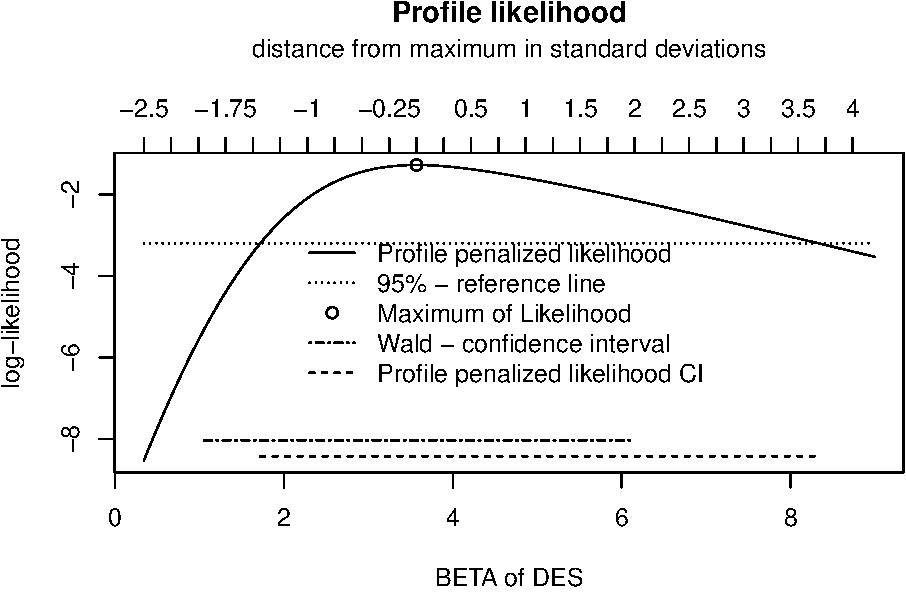
\includegraphics[keepaspectratio]{suppMat_files/figure-latex/unnamed-chunk-14-1.pdf}}

\begin{Shaded}
\begin{Highlighting}[]
\NormalTok{beta\_t }\OtherTok{\textless{}{-}}\NormalTok{ fclr[,}\StringTok{"DES"}\NormalTok{]}
\NormalTok{fclr }\OtherTok{\textless{}{-}}\NormalTok{ fclr[,}\StringTok{"log{-}likelihood"}\NormalTok{]}
\NormalTok{uclr }\OtherTok{\textless{}{-}}\NormalTok{ logfu }\OtherTok{\textless{}{-}}\NormalTok{ logfw }\OtherTok{\textless{}{-}} \FunctionTok{rep}\NormalTok{(}\ConstantTok{NA}\NormalTok{,}\FunctionTok{length}\NormalTok{(beta\_t))}
\ControlFlowTok{for}\NormalTok{(i }\ControlFlowTok{in} \FunctionTok{seq\_along}\NormalTok{(beta\_t)) \{}
\NormalTok{  uclr[i] }\OtherTok{\textless{}{-}} \FunctionTok{profile\_ll\_logF}\NormalTok{(beta\_t[i],des.aug0)}
\NormalTok{  logfu[i] }\OtherTok{\textless{}{-}} \FunctionTok{profile\_ll\_logF}\NormalTok{(beta\_t[i],des.augU)}
\NormalTok{  logfw[i] }\OtherTok{\textless{}{-}} \FunctionTok{profile\_ll\_logF}\NormalTok{(beta\_t[i],des.augW)}
\NormalTok{\}}
\NormalTok{mm }\OtherTok{\textless{}{-}} \FunctionTok{factor}\NormalTok{(}\FunctionTok{rep}\NormalTok{(}\FunctionTok{c}\NormalTok{(}\StringTok{"UCLR"}\NormalTok{,}\StringTok{"FCLR"}\NormalTok{,}\StringTok{"logFU"}\NormalTok{,}\StringTok{"logFW"}\NormalTok{),}\AttributeTok{each=}\FunctionTok{length}\NormalTok{(beta\_t)),}
             \AttributeTok{levels=}\FunctionTok{c}\NormalTok{(}\StringTok{"UCLR"}\NormalTok{,}\StringTok{"FCLR"}\NormalTok{,}\StringTok{"logFU"}\NormalTok{,}\StringTok{"logFW"}\NormalTok{))}
\NormalTok{plotdat }\OtherTok{\textless{}{-}} \FunctionTok{data.frame}\NormalTok{(}\AttributeTok{logGRR=}\FunctionTok{rep}\NormalTok{(beta\_t,}\DecValTok{4}\NormalTok{),}\AttributeTok{profll=}\FunctionTok{c}\NormalTok{(uclr,fclr,logfu,logfw),}
                      \AttributeTok{method=}\NormalTok{mm)}
\end{Highlighting}
\end{Shaded}

Finally, we can plot the curves.

\begin{Shaded}
\begin{Highlighting}[]
\FunctionTok{ggplot}\NormalTok{(plotdat,}\FunctionTok{aes}\NormalTok{(}\AttributeTok{x=}\NormalTok{logGRR,}\AttributeTok{y=}\NormalTok{profll,}\AttributeTok{color=}\NormalTok{method)) }\SpecialCharTok{+} \FunctionTok{geom\_line}\NormalTok{() }\SpecialCharTok{+}
   \FunctionTok{scale\_color\_manual}\NormalTok{(}\AttributeTok{values=}\FunctionTok{c}\NormalTok{(}\StringTok{"black"}\NormalTok{,}\StringTok{"\#00AFBB"}\NormalTok{,}\StringTok{"\#52854C"}\NormalTok{,}\StringTok{"\#E7B800"}\NormalTok{)) }\SpecialCharTok{+}
  \FunctionTok{xlab}\NormalTok{(}\FunctionTok{expression}\NormalTok{(}\FunctionTok{paste}\NormalTok{(}\StringTok{"log{-}OR "}\NormalTok{,beta))) }\SpecialCharTok{+} 
  \FunctionTok{ylab}\NormalTok{(}\StringTok{"Profile penalized log{-}likelihood"}\NormalTok{) }\SpecialCharTok{+}
  \FunctionTok{geom\_vline}\NormalTok{(}\AttributeTok{xintercept=}\NormalTok{beta\_t[}\FunctionTok{which.max}\NormalTok{(fclr)],}
             \AttributeTok{linetype=}\StringTok{"longdash"}\NormalTok{, }\AttributeTok{color=}\StringTok{"\#00AFBB"}\NormalTok{) }\SpecialCharTok{+}
  \FunctionTok{geom\_vline}\NormalTok{(}\AttributeTok{xintercept=}\NormalTok{beta\_t[}\FunctionTok{which.max}\NormalTok{(logfu)],}
             \AttributeTok{linetype=}\StringTok{"longdash"}\NormalTok{, }\AttributeTok{color=}\StringTok{"\#52854C"}\NormalTok{) }\SpecialCharTok{+}
  \FunctionTok{geom\_vline}\NormalTok{(}\AttributeTok{xintercept=}\NormalTok{beta\_t[}\FunctionTok{which.max}\NormalTok{(logfw)],}
             \AttributeTok{linetype=}\StringTok{"longdash"}\NormalTok{, }\AttributeTok{color=}\StringTok{"\#E7B800"}\NormalTok{)}
\end{Highlighting}
\end{Shaded}

\pandocbounded{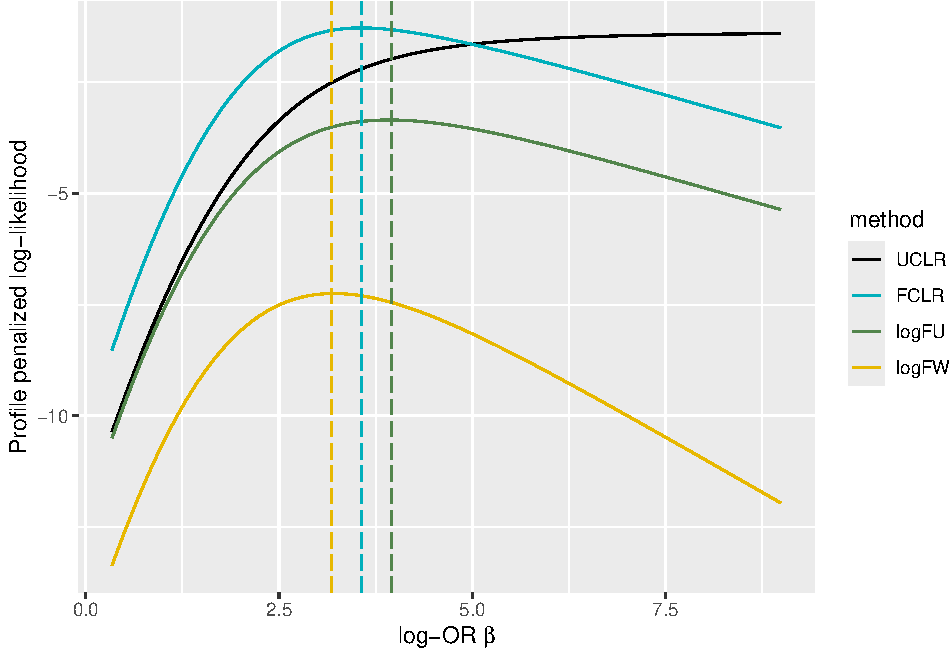
\includegraphics[keepaspectratio]{suppMat_files/figure-latex/unnamed-chunk-15-1.pdf}}

\begin{Shaded}
\begin{Highlighting}[]
\FunctionTok{ggsave}\NormalTok{(}\AttributeTok{file=}\StringTok{"DESprofile.eps"}\NormalTok{,}\AttributeTok{device=}\StringTok{"eps"}\NormalTok{)}
\end{Highlighting}
\end{Shaded}

\begin{verbatim}
## Saving 6.5 x 4.5 in image
\end{verbatim}

\begin{Shaded}
\begin{Highlighting}[]
\FunctionTok{ggsave}\NormalTok{(}\AttributeTok{file=}\StringTok{"DESprofile.pdf"}\NormalTok{,}\AttributeTok{device=}\StringTok{"pdf"}\NormalTok{)}
\end{Highlighting}
\end{Shaded}

\begin{verbatim}
## Saving 6.5 x 4.5 in image
\end{verbatim}

\subsection{Session information for DES
analysis}\label{session-information-for-des-analysis}

\begin{Shaded}
\begin{Highlighting}[]
\FunctionTok{sessionInfo}\NormalTok{()}
\end{Highlighting}
\end{Shaded}

\begin{verbatim}
## R version 4.4.1 (2024-06-14)
## Platform: aarch64-apple-darwin20
## Running under: macOS Sonoma 14.7.8
## 
## Matrix products: default
## BLAS:   /Library/Frameworks/R.framework/Versions/4.4-arm64/Resources/lib/libRblas.0.dylib 
## LAPACK: /Library/Frameworks/R.framework/Versions/4.4-arm64/Resources/lib/libRlapack.dylib;  LAPACK version 3.12.0
## 
## locale:
## [1] en_US.UTF-8/en_US.UTF-8/en_US.UTF-8/C/en_US.UTF-8/en_US.UTF-8
## 
## time zone: America/Vancouver
## tzcode source: internal
## 
## attached base packages:
## [1] stats     graphics  grDevices utils     datasets  methods   base     
## 
## other attached packages:
##  [1] lubridate_1.9.3 forcats_1.0.0   stringr_1.5.1   dplyr_1.2.0    
##  [5] purrr_1.0.2     readr_2.1.5     tidyr_1.3.2     tibble_3.2.1   
##  [9] ggplot2_4.0.2   tidyverse_2.0.0 coxphf_1.13.4   survival_3.6-4 
## 
## loaded via a namespace (and not attached):
##  [1] Matrix_1.7-0       gtable_0.3.6       compiler_4.4.1     tinytex_0.51      
##  [5] tidyselect_1.2.1   textshaping_0.4.0  systemfonts_1.3.2  splines_4.4.1     
##  [9] scales_1.4.0       yaml_2.3.8         fastmap_1.2.0      lattice_0.22-6    
## [13] R6_2.5.1           labeling_0.4.3     generics_0.1.3     knitr_1.50        
## [17] pillar_1.11.1      RColorBrewer_1.1-3 tzdb_0.5.0         rlang_1.1.7       
## [21] stringi_1.8.4      xfun_0.52          S7_0.2.1           timechange_0.3.0  
## [25] cli_3.6.4          withr_3.0.0        magrittr_2.0.3     digest_0.6.37     
## [29] grid_4.4.1         rstudioapi_0.16.0  hms_1.1.3          lifecycle_1.0.5   
## [33] vctrs_0.7.2        evaluate_1.0.1     glue_1.8.0         farver_2.1.2      
## [37] ragg_1.3.2         rmarkdown_2.27     tools_4.4.1        pkgconfig_2.0.3   
## [41] htmltools_0.5.8.1
\end{verbatim}

\clearpage

\section{Trio data analysis}\label{trio-data-analysis}

\subsection{Purpose}\label{purpose}

This document reconstructs the case-parent trio analysis used in the
manuscript. It explains the conditional-likelihood formulation, shows
how Mendelian transmission probabilities enter as offsets in conditional
logistic regression, and fits an additive per-allele model for the Z+2
allele at the \textit{GCK1} microsatellite locus.

The reconstructed data are based on the counts reported by Frayling et
al.~(1999). The affected child is treated as the case, and the genotypes
that could have been transmitted by the same parents are treated as
matched pseudo-controls. Parental mating type defines the matched set.

\subsection{Data and notation}\label{data-and-notation}

Let

\begin{itemize}
\tightlist
\item
  \(G\in\{0,1,2\}\) denote the number of copies of the Z+2 allele
  carried by the child;
\item
  \(G_p=(g_{p1},g_{p2})\) denote the parental Z+2 allele counts;
\item
  \(D=1\) identify the observed affected child and \(D=0\) identify a
  pseudo-control genotype.
\end{itemize}

The original draft described the genetic variants as SNPs. That is not
correct for this application: \textit{GCK1} is a microsatellite locus,
and Z+2 is one of its alleles.

The reported affected-child counts are:

\begin{Shaded}
\begin{Highlighting}[]
\NormalTok{affected\_counts }\OtherTok{\textless{}{-}} \FunctionTok{data.frame}\NormalTok{(}
  \AttributeTok{mating =} \FunctionTok{c}\NormalTok{(}\StringTok{"0x1"}\NormalTok{, }\StringTok{"0x1"}\NormalTok{, }\StringTok{"1x1"}\NormalTok{, }\StringTok{"1x1"}\NormalTok{),}
  \AttributeTok{observed\_g =} \FunctionTok{c}\NormalTok{(}\DecValTok{0}\NormalTok{, }\DecValTok{1}\NormalTok{, }\DecValTok{0}\NormalTok{, }\DecValTok{1}\NormalTok{),}
  \AttributeTok{n =} \FunctionTok{c}\NormalTok{(}\DecValTok{10}\NormalTok{, }\DecValTok{15}\NormalTok{, }\DecValTok{1}\NormalTok{, }\DecValTok{1}\NormalTok{)}
\NormalTok{)}

\NormalTok{affected\_counts}
\end{Highlighting}
\end{Shaded}

\begin{verbatim}
##   mating observed_g  n
## 1    0x1          0 10
## 2    0x1          1 15
## 3    1x1          0  1
## 4    1x1          1  1
\end{verbatim}

\subsection{Conditional likelihood for trio
data}\label{conditional-likelihood-for-trio-data}

Conditional on parental mating type \(G_p\), the probability that the
affected child has genotype \(g\) is proportional to

\[
\exp\{z(g)^T\beta\}P(G=g\mid G_p),
\]

where \(P(G=g\mid G_p)\) is the Mendelian transmission probability. Thus
the likelihood contribution of one trio is

\[
\frac{
  \exp\{z(g)^T\beta\}P(G=g\mid G_p)
}{
  \sum_{g^\ast}
  \exp\{z(g^\ast)^T\beta\}P(G=g^\ast\mid G_p)
}.
\]

This has the form of a conditional logistic likelihood with linear
predictor

\[
z(g)^T\beta+\log P(G=g\mid G_p).
\]

Therefore, the logarithm of the Mendelian transmission probability
enters the conditional logistic regression as an offset.

Because an additive constant within a matched set cancels from the
conditional likelihood, one may use either the exact log probabilities
or any proportional weights. For a \(1\times1\) mating, for example,

\[
P(G=0\mid G_p)=\frac14,\qquad
P(G=1\mid G_p)=\frac12,\qquad
P(G=2\mid G_p)=\frac14.
\]

The exact offsets are \(\{\log(1/4),\log(1/2),\log(1/4)\}\). Subtracting
the common value \(\log(1/4)\) gives the equivalent offsets

\[
\{0,\log 2,0\}.
\]

\subsubsection{Additive per-allele
model}\label{additive-per-allele-model}

The manuscript reports a single genotype relative risk for each
additional copy of the Z+2 allele. The corresponding model is

\[
z(g)=g
\]

and

\[
\operatorname{GRR}=\exp(\beta).
\]

This is different from a two-parameter model with separate genotype
effects. If one writes

\[
z(g)=
\begin{cases}
(0,0), & g=0,\\
(1,0), & g=1,\\
(1,1), & g=2,
\end{cases}
\]

then the parameters are log relative-risk increments:

\[
\exp(\beta_1)
=
\frac{P(D=1\mid G=1)}{P(D=1\mid G=0)},
\qquad
\exp(\beta_2)
=
\frac{P(D=1\mid G=2)}{P(D=1\mid G=1)}.
\]

The \(\beta_j\) themselves are log-GRRs, not GRRs. In these
reconstructed data, no affected child has genotype \(G=2\), so the
two-parameter model has no information about \(\beta_2\). The
single-parameter additive model is therefore the model used below.

\subsection{Reconstructing the matched pseudo-control
data}\label{reconstructing-the-matched-pseudo-control-data}

For a \(0\times1\) mating, the possible offspring genotypes are 0 and 1,
each with probability \(1/2\).

For a \(1\times1\) mating, the possible offspring genotypes are 0, 1,
and 2, with probabilities \(1/4\), \(1/2\), and \(1/4\), respectively.

Each observed affected child defines one matched set. The observed
genotype is coded as the case, and the other possible offspring
genotypes are coded as pseudo-controls.

\begin{Shaded}
\begin{Highlighting}[]
\NormalTok{make\_set }\OtherTok{\textless{}{-}} \ControlFlowTok{function}\NormalTok{(stratum, mating, observed\_g) \{}
  \ControlFlowTok{if}\NormalTok{ (mating }\SpecialCharTok{==} \StringTok{"0x1"}\NormalTok{) \{}
    \CommentTok{\# Mendelian probabilities: P(G=0)=1/2, P(G=1)=1/2}
\NormalTok{    g }\OtherTok{\textless{}{-}} \FunctionTok{c}\NormalTok{(}\DecValTok{0}\NormalTok{, }\DecValTok{1}\NormalTok{)}

\NormalTok{  \} }\ControlFlowTok{else} \ControlFlowTok{if}\NormalTok{ (mating }\SpecialCharTok{==} \StringTok{"1x1"}\NormalTok{) \{}
    \CommentTok{\# Mendelian probabilities: P(G=0)=1/4, P(G=1)=1/2, P(G=2)=1/4}
    \CommentTok{\# Represent these probabilities by multiplicities 1:2:1.}
\NormalTok{    g }\OtherTok{\textless{}{-}} \FunctionTok{c}\NormalTok{(}\DecValTok{0}\NormalTok{, }\DecValTok{1}\NormalTok{, }\DecValTok{1}\NormalTok{, }\DecValTok{2}\NormalTok{)}

\NormalTok{  \} }\ControlFlowTok{else}\NormalTok{ \{}
    \FunctionTok{stop}\NormalTok{(}\StringTok{"Unsupported mating type: "}\NormalTok{, mating)}
\NormalTok{  \}}

\NormalTok{  case }\OtherTok{\textless{}{-}} \FunctionTok{integer}\NormalTok{(}\FunctionTok{length}\NormalTok{(g))}

  \CommentTok{\# Mark exactly one copy of the observed genotype as the affected child.}
\NormalTok{  observed\_rows }\OtherTok{\textless{}{-}} \FunctionTok{which}\NormalTok{(g }\SpecialCharTok{==}\NormalTok{ observed\_g)}

  \ControlFlowTok{if}\NormalTok{ (}\FunctionTok{length}\NormalTok{(observed\_rows) }\SpecialCharTok{==} \DecValTok{0}\DataTypeTok{L}\NormalTok{) \{}
    \FunctionTok{stop}\NormalTok{(}
      \StringTok{"Observed genotype "}\NormalTok{, observed\_g,}
      \StringTok{" is incompatible with mating type "}\NormalTok{, mating, }\StringTok{"."}
\NormalTok{    )}
\NormalTok{  \}}

\NormalTok{  case[observed\_rows[}\DecValTok{1}\DataTypeTok{L}\NormalTok{]] }\OtherTok{\textless{}{-}} \DecValTok{1}\DataTypeTok{L}

  \FunctionTok{data.frame}\NormalTok{(}
    \AttributeTok{stratum =}\NormalTok{ stratum,}
    \AttributeTok{mating =}\NormalTok{ mating,}
    \AttributeTok{g =}\NormalTok{ g,}
    \AttributeTok{case =}\NormalTok{ case}
\NormalTok{  )}
\NormalTok{\}}

\NormalTok{sets }\OtherTok{\textless{}{-}} \FunctionTok{vector}\NormalTok{(}\StringTok{"list"}\NormalTok{, }\FunctionTok{sum}\NormalTok{(affected\_counts}\SpecialCharTok{$}\NormalTok{n))}
\NormalTok{s }\OtherTok{\textless{}{-}} \DecValTok{1}\DataTypeTok{L}

\ControlFlowTok{for}\NormalTok{ (i }\ControlFlowTok{in} \FunctionTok{seq\_len}\NormalTok{(}\FunctionTok{nrow}\NormalTok{(affected\_counts))) \{}
  \ControlFlowTok{for}\NormalTok{ (j }\ControlFlowTok{in} \FunctionTok{seq\_len}\NormalTok{(affected\_counts}\SpecialCharTok{$}\NormalTok{n[i])) \{}
\NormalTok{    sets[[s]] }\OtherTok{\textless{}{-}} \FunctionTok{make\_set}\NormalTok{(}
      \AttributeTok{stratum =}\NormalTok{ s,}
      \AttributeTok{mating =}\NormalTok{ affected\_counts}\SpecialCharTok{$}\NormalTok{mating[i],}
      \AttributeTok{observed\_g =}\NormalTok{ affected\_counts}\SpecialCharTok{$}\NormalTok{observed\_g[i]}
\NormalTok{    )}
\NormalTok{    s }\OtherTok{\textless{}{-}}\NormalTok{ s }\SpecialCharTok{+} \DecValTok{1}\DataTypeTok{L}
\NormalTok{  \}}
\NormalTok{\}}

\NormalTok{trio\_dat }\OtherTok{\textless{}{-}} \FunctionTok{do.call}\NormalTok{(rbind, sets)}
\FunctionTok{row.names}\NormalTok{(trio\_dat) }\OtherTok{\textless{}{-}} \ConstantTok{NULL}

\FunctionTok{head}\NormalTok{(trio\_dat, }\DecValTok{12}\NormalTok{)}
\end{Highlighting}
\end{Shaded}

\begin{verbatim}
##    stratum mating g case
## 1        1    0x1 0    1
## 2        1    0x1 1    0
## 3        2    0x1 0    1
## 4        2    0x1 1    0
## 5        3    0x1 0    1
## 6        3    0x1 1    0
## 7        4    0x1 0    1
## 8        4    0x1 1    0
## 9        5    0x1 0    1
## 10       5    0x1 1    0
## 11       6    0x1 0    1
## 12       6    0x1 1    0
\end{verbatim}

Basic checks:

\begin{Shaded}
\begin{Highlighting}[]
\FunctionTok{stopifnot}\NormalTok{(}\FunctionTok{all}\NormalTok{(}\FunctionTok{tapply}\NormalTok{(trio\_dat}\SpecialCharTok{$}\NormalTok{case, trio\_dat}\SpecialCharTok{$}\NormalTok{stratum, sum) }\SpecialCharTok{==} \DecValTok{1}\NormalTok{))}
\FunctionTok{stopifnot}\NormalTok{(}\FunctionTok{nlevels}\NormalTok{(}\FunctionTok{factor}\NormalTok{(trio\_dat}\SpecialCharTok{$}\NormalTok{stratum)) }\SpecialCharTok{==} \DecValTok{27}\NormalTok{)}
\FunctionTok{stopifnot}\NormalTok{(}\FunctionTok{nrow}\NormalTok{(trio\_dat) }\SpecialCharTok{==} \DecValTok{58}\NormalTok{)}

\FunctionTok{with}\NormalTok{(trio\_dat, }\FunctionTok{table}\NormalTok{(mating, g, case))}
\end{Highlighting}
\end{Shaded}

\begin{verbatim}
## , , case = 0
## 
##       g
## mating  0  1  2
##    0x1 15 10  0
##    1x1  1  3  2
## 
## , , case = 1
## 
##       g
## mating  0  1  2
##    0x1 10 15  0
##    1x1  1  1  0
\end{verbatim}

\subsection{Fitting the additive conditional logistic
regression}\label{fitting-the-additive-conditional-logistic-regression}

\begin{Shaded}
\begin{Highlighting}[]
\FunctionTok{library}\NormalTok{(survival)}

\NormalTok{fit }\OtherTok{\textless{}{-}} \FunctionTok{clogit}\NormalTok{(}
\NormalTok{  case }\SpecialCharTok{\textasciitilde{}}\NormalTok{ g }\SpecialCharTok{+} \FunctionTok{strata}\NormalTok{(stratum),}
  \AttributeTok{data =}\NormalTok{ trio\_dat,}
  \AttributeTok{method =} \StringTok{"exact"}
\NormalTok{)}

\FunctionTok{summary}\NormalTok{(fit)}
\end{Highlighting}
\end{Shaded}

\begin{verbatim}
## Call:
## coxph(formula = Surv(rep(1, 58L), case) ~ g + strata(stratum), 
##     data = trio_dat, method = "exact")
## 
##   n= 58, number of events= 27 
## 
##     coef exp(coef) se(coef)     z Pr(>|z|)
## g 0.2076    1.2308   0.3734 0.556    0.578
## 
##   exp(coef) exp(-coef) lower .95 upper .95
## g     1.231     0.8125     0.592     2.559
## 
## Concordance= 0.532  (se = 0.13 )
## Likelihood ratio test= 0.31  on 1 df,   p=0.6
## Wald test            = 0.31  on 1 df,   p=0.6
## Score (logrank) test = 0.31  on 1 df,   p=0.6
\end{verbatim}

\begin{Shaded}
\begin{Highlighting}[]
\NormalTok{trio\_dat}\SpecialCharTok{$}\NormalTok{matchedset }\OtherTok{\textless{}{-}}\NormalTok{ trio\_dat}\SpecialCharTok{$}\NormalTok{stratum}
\NormalTok{form }\OtherTok{\textless{}{-}} \FunctionTok{formula}\NormalTok{(case }\SpecialCharTok{\textasciitilde{}}\NormalTok{ g)}
\CommentTok{\#trio.aug0 \textless{}{-} augment.logFmatched(form,trio\_dat,m=0) \# doesn\textquotesingle{}t work. Not set up for m=0}
\NormalTok{trio.aug0 }\OtherTok{\textless{}{-}}\NormalTok{ trio\_dat; trio.aug0}\SpecialCharTok{$}\NormalTok{weights }\OtherTok{\textless{}{-}} \DecValTok{1} \CommentTok{\# add weights manually}
\NormalTok{UCLR }\OtherTok{\textless{}{-}} \FunctionTok{clogitlogF}\NormalTok{(form,trio.aug0,}\AttributeTok{maxit=}\DecValTok{500}\NormalTok{)}
\NormalTok{UCLR}
\end{Highlighting}
\end{Shaded}

\begin{verbatim}
## Call:
## clogit(formula, dat, weights = dat$weights, method = "efron", 
##     iter.max = maxit)
## 
##     coef exp(coef) se(coef)     z     p
## g 0.2076    1.2308   0.3734 0.556 0.578
## 
## Likelihood ratio test=0.31  on 1 df, p=0.5771
## n= 58, number of events= 27
\end{verbatim}

\begin{Shaded}
\begin{Highlighting}[]
\FunctionTok{exp}\NormalTok{(}\FunctionTok{c}\NormalTok{(UCLR}\SpecialCharTok{$}\NormalTok{ci.lower,UCLR}\SpecialCharTok{$}\NormalTok{ci.upper))}
\end{Highlighting}
\end{Shaded}

\begin{verbatim}
##     lower     upper 
## 0.5927131 2.6040805
\end{verbatim}

\begin{Shaded}
\begin{Highlighting}[]
\NormalTok{FCLR }\OtherTok{\textless{}{-}} \FunctionTok{clogitf}\NormalTok{(form,trio\_dat,}\AttributeTok{maxit=}\DecValTok{500}\NormalTok{)}
\NormalTok{FCLR}
\end{Highlighting}
\end{Shaded}

\begin{verbatim}
## coxphf(formula = newformula, data = data, pl = pl, alpha = alpha, 
##     maxit = maxit, maxstep = 0.1, firth = firth, penalty = penalty)
## Model fitted by Penalized ML
## Confidence intervals and p-values by Profile Likelihood 
## 
##        coef  se(coef) exp(coef) lower 0.95 upper 0.95    Chisq         p
## g 0.2006707 0.3732617  1.222222  0.5959001   2.551013 0.300502 0.5835679
## 
## Likelihood ratio test=0.300502 on 1 df, p=0.5835679, n=58
\end{verbatim}

\begin{Shaded}
\begin{Highlighting}[]
\FunctionTok{confint}\NormalTok{(FCLR)}
\end{Highlighting}
\end{Shaded}

\begin{verbatim}
##         [,1]      [,2]
## g -0.5176822 0.9364906
\end{verbatim}

\begin{Shaded}
\begin{Highlighting}[]
\FunctionTok{exp}\NormalTok{(}\FunctionTok{confint}\NormalTok{(FCLR))}
\end{Highlighting}
\end{Shaded}

\begin{verbatim}
##        [,1]     [,2]
## g 0.5959001 2.551013
\end{verbatim}

The uninformative prior for the binary genotype effect is log-F(1,1).

\begin{Shaded}
\begin{Highlighting}[]
\NormalTok{trio.augU }\OtherTok{\textless{}{-}} \FunctionTok{augment.logFmatched}\NormalTok{(form,trio\_dat,}\AttributeTok{m=}\DecValTok{1}\NormalTok{)}
\NormalTok{logFU }\OtherTok{\textless{}{-}} \FunctionTok{clogitlogF}\NormalTok{(form,trio.augU)}
\NormalTok{logFU}
\end{Highlighting}
\end{Shaded}

\begin{verbatim}
## Call:
## clogit(formula, dat, weights = dat$weights, method = "efron", 
##     iter.max = maxit)
## 
##     coef exp(coef) se(coef) robust se     z     p
## g 0.2007    1.2222   0.3670    0.2727 0.736 0.462
## 
## Likelihood ratio test=0.3  on 1 df, p=0.5836
## n= 62, number of events= 29
\end{verbatim}

\begin{Shaded}
\begin{Highlighting}[]
\FunctionTok{confint}\NormalTok{(logFU)}
\end{Highlighting}
\end{Shaded}

\begin{verbatim}
##      lower      upper 
## -0.5176824  0.9364907
\end{verbatim}

\begin{Shaded}
\begin{Highlighting}[]
\FunctionTok{exp}\NormalTok{(}\FunctionTok{confint}\NormalTok{(logFU))}
\end{Highlighting}
\end{Shaded}

\begin{verbatim}
##    lower    upper 
## 0.595900 2.551013
\end{verbatim}

The weakly informative prior is log-F(2,2).

\begin{Shaded}
\begin{Highlighting}[]
\NormalTok{trio.augW }\OtherTok{\textless{}{-}} \FunctionTok{augment.logFmatched}\NormalTok{(form,trio\_dat,}\AttributeTok{m=}\DecValTok{2}\NormalTok{)}
\NormalTok{logFW }\OtherTok{\textless{}{-}} \FunctionTok{clogitlogF}\NormalTok{(form,trio.augW)}
\NormalTok{logFW}
\end{Highlighting}
\end{Shaded}

\begin{verbatim}
## Call:
## clogit(formula, dat, weights = dat$weights, method = "efron", 
##     iter.max = maxit)
## 
##     coef exp(coef) se(coef)     z     p
## g 0.1942    1.2143   0.3609 0.538 0.591
## 
## Likelihood ratio test=0.29  on 1 df, p=0.5897
## n= 62, number of events= 29
\end{verbatim}

\begin{Shaded}
\begin{Highlighting}[]
\FunctionTok{confint}\NormalTok{(logFW)}
\end{Highlighting}
\end{Shaded}

\begin{verbatim}
##      lower      upper 
## -0.5124318  0.9171290
\end{verbatim}

\begin{Shaded}
\begin{Highlighting}[]
\FunctionTok{exp}\NormalTok{(}\FunctionTok{confint}\NormalTok{(logFW))}
\end{Highlighting}
\end{Shaded}

\begin{verbatim}
##     lower     upper 
## 0.5990371 2.5020965
\end{verbatim}

\subsection{Session information for the trio data
analysis}\label{session-information-for-the-trio-data-analysis}

\begin{Shaded}
\begin{Highlighting}[]
\FunctionTok{sessionInfo}\NormalTok{()}
\end{Highlighting}
\end{Shaded}

\begin{verbatim}
## R version 4.4.1 (2024-06-14)
## Platform: aarch64-apple-darwin20
## Running under: macOS Sonoma 14.7.8
## 
## Matrix products: default
## BLAS:   /Library/Frameworks/R.framework/Versions/4.4-arm64/Resources/lib/libRblas.0.dylib 
## LAPACK: /Library/Frameworks/R.framework/Versions/4.4-arm64/Resources/lib/libRlapack.dylib;  LAPACK version 3.12.0
## 
## locale:
## [1] en_US.UTF-8/en_US.UTF-8/en_US.UTF-8/C/en_US.UTF-8/en_US.UTF-8
## 
## time zone: America/Vancouver
## tzcode source: internal
## 
## attached base packages:
## [1] stats     graphics  grDevices utils     datasets  methods   base     
## 
## other attached packages:
##  [1] lubridate_1.9.3 forcats_1.0.0   stringr_1.5.1   dplyr_1.2.0    
##  [5] purrr_1.0.2     readr_2.1.5     tidyr_1.3.2     tibble_3.2.1   
##  [9] ggplot2_4.0.2   tidyverse_2.0.0 coxphf_1.13.4   survival_3.6-4 
## 
## loaded via a namespace (and not attached):
##  [1] Matrix_1.7-0       gtable_0.3.6       compiler_4.4.1     tinytex_0.51      
##  [5] tidyselect_1.2.1   textshaping_0.4.0  systemfonts_1.3.2  splines_4.4.1     
##  [9] scales_1.4.0       yaml_2.3.8         fastmap_1.2.0      lattice_0.22-6    
## [13] R6_2.5.1           labeling_0.4.3     generics_0.1.3     knitr_1.50        
## [17] pillar_1.11.1      RColorBrewer_1.1-3 tzdb_0.5.0         rlang_1.1.7       
## [21] stringi_1.8.4      xfun_0.52          S7_0.2.1           timechange_0.3.0  
## [25] cli_3.6.4          withr_3.0.0        magrittr_2.0.3     digest_0.6.37     
## [29] grid_4.4.1         rstudioapi_0.16.0  hms_1.1.3          lifecycle_1.0.5   
## [33] vctrs_0.7.2        evaluate_1.0.1     glue_1.8.0         farver_2.1.2      
## [37] ragg_1.3.2         rmarkdown_2.27     tools_4.4.1        pkgconfig_2.0.3   
## [41] htmltools_0.5.8.1
\end{verbatim}

\clearpage

\section{Complete simulation results}\label{complete-simulation-results}

The full simulation results table is available on GitHub.

\begin{Shaded}
\begin{Highlighting}[]
\NormalTok{results }\OtherTok{\textless{}{-}} \FunctionTok{read.table}\NormalTok{(}\StringTok{"https://raw.githubusercontent.com/SFUStatgen/logF\_CLR/refs/heads/main/simres.txt"}\NormalTok{,}
                      \AttributeTok{header=}\ConstantTok{TRUE}\NormalTok{)}
\end{Highlighting}
\end{Shaded}

% latex table generated in R 4.4.1 by xtable 1.8-4 package
% Wed Jul 29 10:27:36 2026
\begingroup\scriptsize
\begin{longtable}{rrrrrrrrrrrrrrr}
  \toprule
method & nCon & nmatch & exptype & beta & ncov & pfail & bias & bias.SE & MSE & MSE.se & cover & cover.se & test.rej & test.rej.se \\ 
  \midrule
CLR & 1 & 10 & continuous & 0.0 & 0 & 0.0024 & 0.0060 & 0.0097 & 0.9479 & 0.1250 & 0.9321 & 0.0025 & 0.0679 & 0.0025 \\ 
  CLR & 4 & 10 & continuous & 0.0 & 0 & 0.0000 & 0.0016 & 0.0040 & 0.1615 & 0.0030 & 0.9447 & 0.0023 & 0.0553 & 0.0023 \\ 
  CLR & 1 & 20 & continuous & 0.0 & 0 & 0.0000 & -0.0004 & 0.0040 & 0.1616 & 0.0089 & 0.9453 & 0.0023 & 0.0547 & 0.0023 \\ 
  CLR & 4 & 20 & continuous & 0.0 & 0 & 0.0000 & -0.0019 & 0.0026 & 0.0690 & 0.0010 & 0.9467 & 0.0022 & 0.0533 & 0.0022 \\ 
  CLR & 1 & 30 & continuous & 0.0 & 0 & 0.0000 & 0.0022 & 0.0030 & 0.0877 & 0.0016 & 0.9474 & 0.0022 & 0.0526 & 0.0022 \\ 
  CLR & 4 & 30 & continuous & 0.0 & 0 & 0.0000 & -0.0013 & 0.0021 & 0.0445 & 0.0007 & 0.9501 & 0.0022 & 0.0499 & 0.0022 \\ 
  CLR & 1 & 40 & continuous & 0.0 & 0 & 0.0000 & 0.0011 & 0.0025 & 0.0617 & 0.0010 & 0.9466 & 0.0022 & 0.0534 & 0.0022 \\ 
  CLR & 4 & 40 & continuous & 0.0 & 0 & 0.0000 & -0.0020 & 0.0018 & 0.0328 & 0.0005 & 0.9513 & 0.0022 & 0.0487 & 0.0022 \\ 
  CLR & 1 & 50 & continuous & 0.0 & 0 & 0.0000 & -0.0001 & 0.0022 & 0.0467 & 0.0008 & 0.9478 & 0.0022 & 0.0522 & 0.0022 \\ 
  CLR & 4 & 50 & continuous & 0.0 & 0 & 0.0000 & -0.0025 & 0.0016 & 0.0263 & 0.0004 & 0.9495 & 0.0022 & 0.0505 & 0.0022 \\ 
  CLR & 1 & 10 & binary0.05 & 0.0 & 0 & 0.8486 & -0.0041 & 0.0096 & 0.1404 & 0.0074 & 1.0000 & 0.0000 & 0.0000 & 0.0000 \\ 
  CLR & 4 & 10 & binary0.05 & 0.0 & 0 & 0.6024 & 8.2600 & 0.2309 & 280.2258 & 8.6349 & 0.9872 & 0.0018 & 0.0128 & 0.0018 \\ 
  CLR & 1 & 20 & binary0.05 & 0.0 & 0 & 0.4785 & 9.6727 & 0.2228 & 352.3097 & 8.1135 & 0.9996 & 0.0003 & 0.0004 & 0.0003 \\ 
  CLR & 4 & 20 & binary0.05 & 0.0 & 0 & 0.3544 & 1.5922 & 0.0790 & 42.7774 & 2.9105 & 0.9698 & 0.0021 & 0.0302 & 0.0021 \\ 
  CLR & 1 & 30 & binary0.05 & 0.0 & 0 & 0.2978 & 7.0651 & 0.1725 & 258.9297 & 6.2999 & 0.9973 & 0.0006 & 0.0027 & 0.0006 \\ 
  CLR & 4 & 30 & binary0.05 & 0.0 & 0 & 0.2045 & 0.4236 & 0.0324 & 8.5402 & 1.1539 & 0.9697 & 0.0019 & 0.0303 & 0.0019 \\ 
  CLR & 1 & 40 & binary0.05 & 0.0 & 0 & 0.1833 & 4.4626 & 0.1326 & 163.5114 & 4.8166 & 0.9936 & 0.0009 & 0.0064 & 0.0009 \\ 
  CLR & 4 & 40 & binary0.05 & 0.0 & 0 & 0.1290 & 0.0734 & 0.0114 & 1.1428 & 0.3074 & 0.9723 & 0.0018 & 0.0277 & 0.0018 \\ 
  CLR & 1 & 50 & binary0.05 & 0.0 & 0 & 0.1078 & 2.9890 & 0.1063 & 109.7390 & 3.8672 & 0.9664 & 0.0019 & 0.0336 & 0.0019 \\ 
  CLR & 4 & 50 & binary0.05 & 0.0 & 0 & 0.0770 & 0.0012 & 0.0084 & 0.6487 & 0.1465 & 0.9713 & 0.0017 & 0.0287 & 0.0017 \\ 
  CLR & 1 & 10 & binary0.1 & 0.0 & 0 & 0.6524 & 0.0130 & 0.0089 & 0.2782 & 0.0068 & 0.9997 & 0.0003 & 0.0003 & 0.0003 \\ 
  CLR & 4 & 10 & binary0.1 & 0.0 & 0 & 0.3550 & 2.0602 & 0.0937 & 60.8234 & 3.4465 & 0.9781 & 0.0018 & 0.0219 & 0.0018 \\ 
  CLR & 1 & 20 & binary0.1 & 0.0 & 0 & 0.2809 & 1.7131 & 0.0919 & 63.6497 & 3.3307 & 0.9955 & 0.0008 & 0.0045 & 0.0008 \\ 
  CLR & 4 & 20 & binary0.1 & 0.0 & 0 & 0.1186 & 0.1743 & 0.0202 & 3.6256 & 0.6752 & 0.9690 & 0.0018 & 0.0310 & 0.0018 \\ 
  CLR & 1 & 30 & binary0.1 & 0.0 & 0 & 0.1237 & 0.9763 & 0.0636 & 36.4129 & 2.2977 & 0.9777 & 0.0016 & 0.0223 & 0.0016 \\ 
  CLR & 4 & 30 & binary0.1 & 0.0 & 0 & 0.0413 & -0.0384 & 0.0083 & 0.6542 & 0.1410 & 0.9682 & 0.0018 & 0.0318 & 0.0018 \\ 
  CLR & 1 & 40 & binary0.1 & 0.0 & 0 & 0.0536 & 0.2556 & 0.0328 & 10.2710 & 1.1560 & 0.9576 & 0.0021 & 0.0424 & 0.0021 \\ 
  CLR & 4 & 40 & binary0.1 & 0.0 & 0 & 0.0141 & -0.0674 & 0.0066 & 0.4390 & 0.0067 & 0.9562 & 0.0021 & 0.0438 & 0.0021 \\ 
  CLR & 1 & 50 & binary0.1 & 0.0 & 0 & 0.0227 & 0.1347 & 0.0245 & 5.8857 & 0.8491 & 0.9434 & 0.0023 & 0.0566 & 0.0023 \\ 
  CLR & 4 & 50 & binary0.1 & 0.0 & 0 & 0.0043 & -0.0671 & 0.0060 & 0.3605 & 0.0059 & 0.9534 & 0.0021 & 0.0466 & 0.0021 \\ 
  CLR & 1 & 10 & binary0.2 & 0.0 & 0 & 0.3813 & 0.0075 & 0.0087 & 0.4734 & 0.0071 & 0.9989 & 0.0004 & 0.0011 & 0.0004 \\ 
  CLR & 4 & 10 & binary0.2 & 0.0 & 0 & 0.1113 & 0.2605 & 0.0255 & 5.8600 & 0.8805 & 0.9741 & 0.0017 & 0.0259 & 0.0017 \\ 
  CLR & 1 & 20 & binary0.2 & 0.0 & 0 & 0.0930 & 0.0424 & 0.0141 & 1.8165 & 0.4137 & 0.9706 & 0.0018 & 0.0294 & 0.0018 \\ 
  CLR & 4 & 20 & binary0.2 & 0.0 & 0 & 0.0121 & -0.0486 & 0.0081 & 0.6536 & 0.1374 & 0.9558 & 0.0021 & 0.0442 & 0.0021 \\ 
  CLR & 1 & 30 & binary0.2 & 0.0 & 0 & 0.0215 & 0.0041 & 0.0101 & 1.0029 & 0.2308 & 0.9395 & 0.0024 & 0.0605 & 0.0024 \\ 
  CLR & 4 & 30 & binary0.2 & 0.0 & 0 & 0.0012 & -0.0623 & 0.0059 & 0.3571 & 0.0061 & 0.9458 & 0.0023 & 0.0542 & 0.0023 \\ 
  CLR & 1 & 40 & binary0.2 & 0.0 & 0 & 0.0041 & 0.0083 & 0.0068 & 0.4585 & 0.0075 & 0.9391 & 0.0024 & 0.0609 & 0.0024 \\ 
  CLR & 4 & 40 & binary0.2 & 0.0 & 0 & 0.0000 & -0.0343 & 0.0050 & 0.2511 & 0.0040 & 0.9491 & 0.0022 & 0.0509 & 0.0022 \\ 
  CLR & 1 & 50 & binary0.2 & 0.0 & 0 & 0.0005 & -0.0056 & 0.0060 & 0.3579 & 0.0063 & 0.9426 & 0.0023 & 0.0574 & 0.0023 \\ 
  CLR & 4 & 50 & binary0.2 & 0.0 & 0 & 0.0000 & -0.0244 & 0.0044 & 0.1976 & 0.0032 & 0.9469 & 0.0022 & 0.0531 & 0.0022 \\ 
  CLR & 1 & 10 & continuous & 0.5 & 0 & 0.0109 & 0.2630 & 0.0134 & 1.8462 & 0.2698 & 0.9378 & 0.0024 & 0.2072 & 0.0041 \\ 
  CLR & 4 & 10 & continuous & 0.5 & 0 & 0.0000 & 0.0602 & 0.0045 & 0.2055 & 0.0052 & 0.9462 & 0.0023 & 0.2950 & 0.0046 \\ 
  CLR & 1 & 20 & continuous & 0.5 & 0 & 0.0001 & 0.0893 & 0.0049 & 0.2453 & 0.0103 & 0.9407 & 0.0024 & 0.3512 & 0.0048 \\ 
  CLR & 4 & 20 & continuous & 0.5 & 0 & 0.0000 & 0.0234 & 0.0028 & 0.0806 & 0.0013 & 0.9500 & 0.0022 & 0.5127 & 0.0050 \\ 
  CLR & 1 & 30 & continuous & 0.5 & 0 & 0.0000 & 0.0536 & 0.0036 & 0.1302 & 0.0039 & 0.9444 & 0.0023 & 0.4772 & 0.0050 \\ 
  CLR & 4 & 30 & continuous & 0.5 & 0 & 0.0000 & 0.0197 & 0.0023 & 0.0527 & 0.0008 & 0.9479 & 0.0022 & 0.6869 & 0.0046 \\ 
  CLR & 1 & 40 & continuous & 0.5 & 0 & 0.0000 & 0.0413 & 0.0028 & 0.0822 & 0.0018 & 0.9495 & 0.0022 & 0.6008 & 0.0049 \\ 
  CLR & 4 & 40 & continuous & 0.5 & 0 & 0.0000 & 0.0158 & 0.0020 & 0.0383 & 0.0006 & 0.9471 & 0.0022 & 0.8063 & 0.0040 \\ 
  CLR & 1 & 50 & continuous & 0.5 & 0 & 0.0000 & 0.0326 & 0.0025 & 0.0632 & 0.0016 & 0.9498 & 0.0022 & 0.6943 & 0.0046 \\ 
  CLR & 4 & 50 & continuous & 0.5 & 0 & 0.0000 & 0.0066 & 0.0017 & 0.0291 & 0.0004 & 0.9512 & 0.0022 & 0.8814 & 0.0032 \\ 
  CLR & 1 & 10 & binary0.05 & 0.5 & 0 & 0.8074 & -0.4202 & 0.0096 & 0.3557 & 0.0098 & 1.0000 & 0.0000 & 0.0000 & 0.0000 \\ 
  CLR & 4 & 10 & binary0.05 & 0.5 & 0 & 0.4683 & 7.8993 & 0.1991 & 273.2170 & 7.2787 & 0.9947 & 0.0010 & 0.0263 & 0.0022 \\ 
  CLR & 1 & 20 & binary0.05 & 0.5 & 0 & 0.4361 & 7.5779 & 0.1995 & 281.8302 & 7.0974 & 0.9991 & 0.0004 & 0.0007 & 0.0004 \\ 
  CLR & 4 & 20 & binary0.05 & 0.5 & 0 & 0.2051 & 1.7548 & 0.0817 & 56.1379 & 2.9562 & 0.9704 & 0.0019 & 0.0824 & 0.0031 \\ 
  CLR & 1 & 30 & binary0.05 & 0.5 & 0 & 0.2398 & 6.0235 & 0.1575 & 224.8142 & 5.6268 & 0.9951 & 0.0008 & 0.0066 & 0.0009 \\ 
  CLR & 4 & 30 & binary0.05 & 0.5 & 0 & 0.0945 & 0.3177 & 0.0326 & 9.7457 & 1.1447 & 0.9728 & 0.0017 & 0.0950 & 0.0031 \\ 
  CLR & 1 & 40 & binary0.05 & 0.5 & 0 & 0.1310 & 3.7595 & 0.1205 & 140.3758 & 4.3024 & 0.9896 & 0.0011 & 0.0267 & 0.0017 \\ 
  CLR & 4 & 40 & binary0.05 & 0.5 & 0 & 0.0444 & 0.0461 & 0.0182 & 3.1783 & 0.5971 & 0.9649 & 0.0019 & 0.1084 & 0.0032 \\ 
  CLR & 1 & 50 & binary0.05 & 0.5 & 0 & 0.0812 & 2.4723 & 0.0969 & 92.2888 & 3.4664 & 0.9847 & 0.0013 & 0.0663 & 0.0026 \\ 
  CLR & 4 & 50 & binary0.05 & 0.5 & 0 & 0.0210 & -0.0113 & 0.0102 & 1.0253 & 0.2683 & 0.9582 & 0.0020 & 0.1235 & 0.0033 \\ 
  CLR & 1 & 10 & binary0.1 & 0.5 & 0 & 0.5870 & -0.3687 & 0.0090 & 0.4697 & 0.0095 & 0.9995 & 0.0003 & 0.0000 & 0.0000 \\ 
  CLR & 4 & 10 & binary0.1 & 0.5 & 0 & 0.2259 & 1.9896 & 0.0893 & 65.6669 & 3.2243 & 0.9866 & 0.0013 & 0.0563 & 0.0026 \\ 
  CLR & 1 & 20 & binary0.1 & 0.5 & 0 & 0.2480 & 0.7585 & 0.0674 & 34.7739 & 2.3892 & 0.9948 & 0.0008 & 0.0176 & 0.0015 \\ 
  CLR & 4 & 20 & binary0.1 & 0.5 & 0 & 0.0453 & 0.1072 & 0.0210 & 4.2049 & 0.7000 & 0.9632 & 0.0019 & 0.0986 & 0.0031 \\ 
  CLR & 1 & 30 & binary0.1 & 0.5 & 0 & 0.0961 & 0.3685 & 0.0421 & 16.1357 & 1.4771 & 0.9821 & 0.0014 & 0.0600 & 0.0025 \\ 
  CLR & 4 & 30 & binary0.1 & 0.5 & 0 & 0.0087 & -0.0362 & 0.0078 & 0.6085 & 0.1276 & 0.9537 & 0.0021 & 0.1214 & 0.0033 \\ 
  CLR & 1 & 40 & binary0.1 & 0.5 & 0 & 0.0474 & 0.1183 & 0.0220 & 4.6329 & 0.7390 & 0.9670 & 0.0018 & 0.1058 & 0.0032 \\ 
  CLR & 4 & 40 & binary0.1 & 0.5 & 0 & 0.0015 & -0.0447 & 0.0071 & 0.5031 & 0.1333 & 0.9441 & 0.0023 & 0.1417 & 0.0035 \\ 
  CLR & 1 & 50 & binary0.1 & 0.5 & 0 & 0.0223 & 0.0596 & 0.0142 & 1.9803 & 0.4402 & 0.9535 & 0.0021 & 0.1338 & 0.0034 \\ 
  CLR & 4 & 50 & binary0.1 & 0.5 & 0 & 0.0005 & -0.0352 & 0.0054 & 0.2912 & 0.0052 & 0.9445 & 0.0023 & 0.1775 & 0.0038 \\ 
  CLR & 1 & 10 & binary0.2 & 0.5 & 0 & 0.3414 & -0.2572 & 0.0088 & 0.5756 & 0.0093 & 0.9967 & 0.0007 & 0.0036 & 0.0007 \\ 
  CLR & 4 & 10 & binary0.2 & 0.5 & 0 & 0.0512 & 0.1905 & 0.0288 & 7.8949 & 0.9897 & 0.9729 & 0.0017 & 0.0753 & 0.0027 \\ 
  CLR & 1 & 20 & binary0.2 & 0.5 & 0 & 0.0844 & -0.0298 & 0.0107 & 1.0495 & 0.2443 & 0.9782 & 0.0015 & 0.0739 & 0.0027 \\ 
  CLR & 4 & 20 & binary0.2 & 0.5 & 0 & 0.0017 & -0.0209 & 0.0078 & 0.6020 & 0.1333 & 0.9460 & 0.0023 & 0.1260 & 0.0033 \\ 
  CLR & 1 & 30 & binary0.2 & 0.5 & 0 & 0.0212 & 0.0337 & 0.0073 & 0.5297 & 0.0079 & 0.9541 & 0.0021 & 0.1334 & 0.0034 \\ 
  CLR & 4 & 30 & binary0.2 & 0.5 & 0 & 0.0000 & -0.0167 & 0.0054 & 0.2938 & 0.0047 & 0.9489 & 0.0022 & 0.1703 & 0.0038 \\ 
  CLR & 1 & 40 & binary0.2 & 0.5 & 0 & 0.0058 & 0.0417 & 0.0066 & 0.4312 & 0.0069 & 0.9403 & 0.0024 & 0.1656 & 0.0037 \\ 
  CLR & 4 & 40 & binary0.2 & 0.5 & 0 & 0.0000 & -0.0104 & 0.0046 & 0.2087 & 0.0032 & 0.9496 & 0.0022 & 0.2081 & 0.0041 \\ 
  CLR & 1 & 50 & binary0.2 & 0.5 & 0 & 0.0013 & 0.0419 & 0.0057 & 0.3305 & 0.0056 & 0.9428 & 0.0023 & 0.1760 & 0.0038 \\ 
  CLR & 4 & 50 & binary0.2 & 0.5 & 0 & 0.0000 & -0.0063 & 0.0040 & 0.1594 & 0.0024 & 0.9513 & 0.0022 & 0.2410 & 0.0043 \\ 
  CLR & 1 & 10 & continuous & 1.0 & 0 & 0.0622 & 0.4664 & 0.0184 & 3.4073 & 0.3630 & 0.9641 & 0.0019 & 0.5261 & 0.0052 \\ 
  CLR & 4 & 10 & continuous & 1.0 & 0 & 0.0012 & 0.1518 & 0.0074 & 0.5740 & 0.1073 & 0.9414 & 0.0023 & 0.7819 & 0.0041 \\ 
  CLR & 1 & 20 & continuous & 1.0 & 0 & 0.0042 & 0.2571 & 0.0112 & 1.3055 & 0.1704 & 0.9433 & 0.0023 & 0.8446 & 0.0036 \\ 
  CLR & 4 & 20 & continuous & 1.0 & 0 & 0.0000 & 0.0629 & 0.0036 & 0.1354 & 0.0030 & 0.9479 & 0.0022 & 0.9745 & 0.0016 \\ 
  CLR & 1 & 30 & continuous & 1.0 & 0 & 0.0003 & 0.1392 & 0.0055 & 0.3191 & 0.0137 & 0.9446 & 0.0023 & 0.9610 & 0.0019 \\ 
  CLR & 4 & 30 & continuous & 1.0 & 0 & 0.0000 & 0.0389 & 0.0028 & 0.0808 & 0.0016 & 0.9479 & 0.0022 & 0.9984 & 0.0004 \\ 
  CLR & 1 & 40 & continuous & 1.0 & 0 & 0.0000 & 0.0910 & 0.0042 & 0.1821 & 0.0065 & 0.9493 & 0.0022 & 0.9900 & 0.0010 \\ 
  CLR & 4 & 40 & continuous & 1.0 & 0 & 0.0000 & 0.0307 & 0.0024 & 0.0582 & 0.0010 & 0.9496 & 0.0022 & 1.0000 & 0.0000 \\ 
  CLR & 1 & 50 & continuous & 1.0 & 0 & 0.0000 & 0.0773 & 0.0036 & 0.1346 & 0.0052 & 0.9411 & 0.0024 & 0.9978 & 0.0005 \\ 
  CLR & 4 & 50 & continuous & 1.0 & 0 & 0.0000 & 0.0246 & 0.0021 & 0.0445 & 0.0007 & 0.9488 & 0.0022 & 0.9999 & 0.0001 \\ 
  CLR & 1 & 10 & binary0.05 & 1.0 & 0 & 0.7753 & -0.8151 & 0.0101 & 0.8935 & 0.0171 & 0.9902 & 0.0021 & 0.0000 & 0.0000 \\ 
  CLR & 4 & 10 & binary0.05 & 1.0 & 0 & 0.3339 & 8.3030 & 0.1836 & 293.3274 & 6.5636 & 0.9979 & 0.0006 & 0.0555 & 0.0028 \\ 
  CLR & 1 & 20 & binary0.05 & 1.0 & 0 & 0.4175 & 5.8349 & 0.1809 & 224.6186 & 6.2948 & 0.9780 & 0.0019 & 0.0093 & 0.0013 \\ 
  CLR & 4 & 20 & binary0.05 & 1.0 & 0 & 0.1011 & 2.0846 & 0.0878 & 73.7018 & 3.1251 & 0.9687 & 0.0018 & 0.1834 & 0.0041 \\ 
  CLR & 1 & 30 & binary0.05 & 1.0 & 0 & 0.2540 & 4.0931 & 0.1378 & 158.4294 & 4.8256 & 0.9677 & 0.0020 & 0.0373 & 0.0022 \\ 
  CLR & 4 & 30 & binary0.05 & 1.0 & 0 & 0.0322 & 0.4009 & 0.0390 & 14.9086 & 1.3640 & 0.9582 & 0.0020 & 0.2603 & 0.0045 \\ 
  CLR & 1 & 40 & binary0.05 & 1.0 & 0 & 0.1739 & 2.3446 & 0.1021 & 91.6693 & 3.5832 & 0.9616 & 0.0021 & 0.1100 & 0.0034 \\ 
  CLR & 4 & 40 & binary0.05 & 1.0 & 0 & 0.0097 & 0.0957 & 0.0211 & 4.4180 & 0.7048 & 0.9498 & 0.0022 & 0.3242 & 0.0047 \\ 
  CLR & 1 & 50 & binary0.05 & 1.0 & 0 & 0.1145 & 1.5235 & 0.0800 & 58.9259 & 2.8157 & 0.9691 & 0.0018 & 0.1895 & 0.0042 \\ 
  CLR & 4 & 50 & binary0.05 & 1.0 & 0 & 0.0022 & 0.0219 & 0.0136 & 1.8500 & 0.4248 & 0.9452 & 0.0023 & 0.3808 & 0.0049 \\ 
  CLR & 1 & 10 & binary0.1 & 1.0 & 0 & 0.5749 & -0.6639 & 0.0095 & 0.8224 & 0.0153 & 0.9760 & 0.0023 & 0.0019 & 0.0007 \\ 
  CLR & 4 & 10 & binary0.1 & 1.0 & 0 & 0.1443 & 1.7469 & 0.0836 & 62.7912 & 2.9627 & 0.9876 & 0.0012 & 0.1280 & 0.0036 \\ 
  CLR & 1 & 20 & binary0.1 & 1.0 & 0 & 0.2708 & -0.0009 & 0.0400 & 11.6587 & 1.3709 & 0.9615 & 0.0023 & 0.0672 & 0.0029 \\ 
  CLR & 4 & 20 & binary0.1 & 1.0 & 0 & 0.0127 & 0.2438 & 0.0314 & 9.7836 & 1.0860 & 0.9556 & 0.0021 & 0.2771 & 0.0045 \\ 
  CLR & 1 & 30 & binary0.1 & 1.0 & 0 & 0.1423 & 0.0318 & 0.0247 & 5.2209 & 0.8271 & 0.9698 & 0.0018 & 0.1975 & 0.0043 \\ 
  CLR & 4 & 30 & binary0.1 & 1.0 & 0 & 0.0013 & 0.0112 & 0.0098 & 0.9505 & 0.2563 & 0.9447 & 0.0023 & 0.3841 & 0.0049 \\ 
  CLR & 1 & 40 & binary0.1 & 1.0 & 0 & 0.0675 & 0.0207 & 0.0112 & 1.1735 & 0.3025 & 0.9725 & 0.0017 & 0.3127 & 0.0048 \\ 
  CLR & 4 & 40 & binary0.1 & 1.0 & 0 & 0.0001 & -0.0050 & 0.0075 & 0.5648 & 0.1807 & 0.9453 & 0.0023 & 0.4766 & 0.0050 \\ 
  CLR & 1 & 50 & binary0.1 & 1.0 & 0 & 0.0371 & 0.0509 & 0.0078 & 0.5893 & 0.1305 & 0.9669 & 0.0018 & 0.3930 & 0.0050 \\ 
  CLR & 4 & 50 & binary0.1 & 1.0 & 0 & 0.0000 & -0.0035 & 0.0048 & 0.2320 & 0.0038 & 0.9468 & 0.0022 & 0.5717 & 0.0049 \\ 
  CLR & 1 & 10 & binary0.2 & 1.0 & 0 & 0.3816 & -0.4701 & 0.0089 & 0.7120 & 0.0133 & 0.9641 & 0.0024 & 0.0158 & 0.0016 \\ 
  CLR & 4 & 10 & binary0.2 & 1.0 & 0 & 0.0349 & 0.3415 & 0.0372 & 13.4797 & 1.2944 & 0.9660 & 0.0018 & 0.2121 & 0.0042 \\ 
  CLR & 1 & 20 & binary0.2 & 1.0 & 0 & 0.1188 & -0.0774 & 0.0077 & 0.5338 & 0.0081 & 0.9687 & 0.0019 & 0.2162 & 0.0044 \\ 
  CLR & 4 & 20 & binary0.2 & 1.0 & 0 & 0.0007 & 0.0113 & 0.0091 & 0.8206 & 0.2223 & 0.9464 & 0.0023 & 0.3867 & 0.0049 \\ 
  CLR & 1 & 30 & binary0.2 & 1.0 & 0 & 0.0398 & 0.0313 & 0.0071 & 0.4811 & 0.0066 & 0.9668 & 0.0018 & 0.3615 & 0.0049 \\ 
  CLR & 4 & 30 & binary0.2 & 1.0 & 0 & 0.0000 & 0.0338 & 0.0081 & 0.6534 & 0.2223 & 0.9478 & 0.0022 & 0.5445 & 0.0050 \\ 
  CLR & 1 & 40 & binary0.2 & 1.0 & 0 & 0.0156 & 0.0597 & 0.0064 & 0.4052 & 0.0062 & 0.9558 & 0.0021 & 0.4612 & 0.0050 \\ 
  CLR & 4 & 40 & binary0.2 & 1.0 & 0 & 0.0000 & 0.0065 & 0.0044 & 0.1925 & 0.0030 & 0.9488 & 0.0022 & 0.6514 & 0.0048 \\ 
  CLR & 1 & 50 & binary0.2 & 1.0 & 0 & 0.0043 & 0.0651 & 0.0059 & 0.3458 & 0.0058 & 0.9459 & 0.0023 & 0.5394 & 0.0050 \\ 
  CLR & 4 & 50 & binary0.2 & 1.0 & 0 & 0.0000 & 0.0041 & 0.0039 & 0.1552 & 0.0023 & 0.9453 & 0.0023 & 0.7453 & 0.0044 \\ 
  CLR & 1 & 10 & continuous & 1.5 & 0 & 0.1793 & 0.6184 & 0.0255 & 5.7215 & 0.4662 & 0.9771 & 0.0017 & 0.8098 & 0.0043 \\ 
  CLR & 4 & 10 & continuous & 1.5 & 0 & 0.0090 & 0.3436 & 0.0130 & 1.7965 & 0.2179 & 0.9477 & 0.0022 & 0.9761 & 0.0015 \\ 
  CLR & 1 & 20 & continuous & 1.5 & 0 & 0.0339 & 0.5411 & 0.0205 & 4.3589 & 0.4112 & 0.9552 & 0.0021 & 0.9916 & 0.0009 \\ 
  CLR & 4 & 20 & continuous & 1.5 & 0 & 0.0001 & 0.1366 & 0.0055 & 0.3259 & 0.0118 & 0.9407 & 0.0024 & 0.9999 & 0.0001 \\ 
  CLR & 1 & 30 & continuous & 1.5 & 0 & 0.0059 & 0.3443 & 0.0131 & 1.8191 & 0.2036 & 0.9408 & 0.0024 & 0.9998 & 0.0001 \\ 
  CLR & 4 & 30 & continuous & 1.5 & 0 & 0.0000 & 0.0776 & 0.0040 & 0.1674 & 0.0044 & 0.9433 & 0.0023 & 1.0000 & 0.0000 \\ 
  CLR & 1 & 40 & continuous & 1.5 & 0 & 0.0012 & 0.2343 & 0.0087 & 0.8192 & 0.1017 & 0.9416 & 0.0023 & 1.0000 & 0.0000 \\ 
  CLR & 4 & 40 & continuous & 1.5 & 0 & 0.0000 & 0.0567 & 0.0032 & 0.1072 & 0.0021 & 0.9464 & 0.0023 & 1.0000 & 0.0000 \\ 
  CLR & 1 & 50 & continuous & 1.5 & 0 & 0.0005 & 0.1548 & 0.0059 & 0.3672 & 0.0168 & 0.9468 & 0.0022 & 1.0000 & 0.0000 \\ 
  CLR & 4 & 50 & continuous & 1.5 & 0 & 0.0000 & 0.0422 & 0.0028 & 0.0815 & 0.0016 & 0.9482 & 0.0022 & 1.0000 & 0.0000 \\ 
  CLR & 1 & 10 & binary0.05 & 1.5 & 0 & 0.7715 & -1.2006 & 0.0112 & 1.7256 & 0.0270 & 0.9886 & 0.0022 & 0.0004 & 0.0004 \\ 
  CLR & 4 & 10 & binary0.05 & 1.5 & 0 & 0.2417 & 8.7108 & 0.1760 & 310.6841 & 6.1631 & 0.9985 & 0.0004 & 0.1124 & 0.0036 \\ 
  CLR & 1 & 20 & binary0.05 & 1.5 & 0 & 0.4808 & 3.1135 & 0.1547 & 133.9823 & 5.2747 & 0.9721 & 0.0023 & 0.0372 & 0.0026 \\ 
  CLR & 4 & 20 & binary0.05 & 1.5 & 0 & 0.0391 & 2.6888 & 0.0966 & 96.8998 & 3.3864 & 0.9570 & 0.0021 & 0.3804 & 0.0050 \\ 
  CLR & 1 & 30 & binary0.05 & 1.5 & 0 & 0.3387 & 1.7861 & 0.1067 & 78.4841 & 3.6696 & 0.9704 & 0.0021 & 0.1700 & 0.0046 \\ 
  CLR & 4 & 30 & binary0.05 & 1.5 & 0 & 0.0074 & 0.7863 & 0.0528 & 28.2679 & 1.8397 & 0.9517 & 0.0022 & 0.5251 & 0.0050 \\ 
  CLR & 1 & 40 & binary0.05 & 1.5 & 0 & 0.2438 & 1.0099 & 0.0767 & 45.4497 & 2.6440 & 0.9681 & 0.0020 & 0.3265 & 0.0054 \\ 
  CLR & 4 & 40 & binary0.05 & 1.5 & 0 & 0.0011 & 0.2776 & 0.0308 & 9.5597 & 1.0584 & 0.9444 & 0.0023 & 0.6576 & 0.0047 \\ 
  CLR & 1 & 50 & binary0.05 & 1.5 & 0 & 0.1792 & 0.3885 & 0.0479 & 18.9823 & 1.6516 & 0.9706 & 0.0019 & 0.4822 & 0.0055 \\ 
  CLR & 4 & 50 & binary0.05 & 1.5 & 0 & 0.0004 & 0.0855 & 0.0166 & 2.7631 & 0.5411 & 0.9424 & 0.0023 & 0.7380 & 0.0044 \\ 
  CLR & 1 & 10 & binary0.1 & 1.5 & 0 & 0.6003 & -0.9344 & 0.0100 & 1.2708 & 0.0220 & 0.9775 & 0.0023 & 0.0073 & 0.0013 \\ 
  CLR & 4 & 10 & binary0.1 & 1.5 & 0 & 0.1271 & 1.7590 & 0.0852 & 66.4213 & 2.9731 & 0.9848 & 0.0013 & 0.2720 & 0.0048 \\ 
  CLR & 1 & 20 & binary0.1 & 1.5 & 0 & 0.3182 & -0.3028 & 0.0251 & 4.3767 & 0.8188 & 0.9645 & 0.0022 & 0.2171 & 0.0050 \\ 
  CLR & 4 & 20 & binary0.1 & 1.5 & 0 & 0.0105 & 0.3755 & 0.0362 & 13.1206 & 1.2499 & 0.9533 & 0.0021 & 0.5783 & 0.0050 \\ 
  CLR & 1 & 30 & binary0.1 & 1.5 & 0 & 0.1793 & -0.1328 & 0.0094 & 0.7502 & 0.2101 & 0.9708 & 0.0019 & 0.4878 & 0.0055 \\ 
  CLR & 4 & 30 & binary0.1 & 1.5 & 0 & 0.0009 & 0.1178 & 0.0194 & 3.7567 & 0.6455 & 0.9452 & 0.0023 & 0.7392 & 0.0044 \\ 
  CLR & 1 & 40 & binary0.1 & 1.5 & 0 & 0.1059 & -0.0258 & 0.0069 & 0.4281 & 0.0055 & 0.9715 & 0.0018 & 0.6409 & 0.0051 \\ 
  CLR & 4 & 40 & binary0.1 & 1.5 & 0 & 0.0000 & 0.0258 & 0.0064 & 0.4089 & 0.1242 & 0.9485 & 0.0022 & 0.8491 & 0.0036 \\ 
  CLR & 1 & 50 & binary0.1 & 1.5 & 0 & 0.0578 & 0.0574 & 0.0065 & 0.4065 & 0.0053 & 0.9745 & 0.0016 & 0.7609 & 0.0044 \\ 
  CLR & 4 & 50 & binary0.1 & 1.5 & 0 & 0.0000 & 0.0170 & 0.0046 & 0.2149 & 0.0034 & 0.9466 & 0.0022 & 0.9217 & 0.0027 \\ 
  CLR & 1 & 10 & binary0.2 & 1.5 & 0 & 0.4342 & -0.6430 & 0.0088 & 0.8557 & 0.0170 & 0.9647 & 0.0025 & 0.0613 & 0.0032 \\ 
  CLR & 4 & 10 & binary0.2 & 1.5 & 0 & 0.0580 & 0.6365 & 0.0505 & 24.4673 & 1.7568 & 0.9654 & 0.0019 & 0.4293 & 0.0051 \\ 
  CLR & 1 & 20 & binary0.2 & 1.5 & 0 & 0.1919 & -0.1500 & 0.0073 & 0.4524 & 0.0075 & 0.9694 & 0.0019 & 0.4746 & 0.0056 \\ 
  CLR & 4 & 20 & binary0.2 & 1.5 & 0 & 0.0032 & 0.1087 & 0.0164 & 2.6956 & 0.5333 & 0.9489 & 0.0022 & 0.7274 & 0.0045 \\ 
  CLR & 1 & 30 & binary0.2 & 1.5 & 0 & 0.0848 & 0.0195 & 0.0068 & 0.4249 & 0.0052 & 0.9715 & 0.0017 & 0.6906 & 0.0048 \\ 
  CLR & 4 & 30 & binary0.2 & 1.5 & 0 & 0.0004 & 0.0251 & 0.0053 & 0.2795 & 0.0047 & 0.9477 & 0.0022 & 0.8787 & 0.0033 \\ 
  CLR & 1 & 40 & binary0.2 & 1.5 & 0 & 0.0372 & 0.0700 & 0.0064 & 0.3998 & 0.0055 & 0.9731 & 0.0016 & 0.8110 & 0.0040 \\ 
  CLR & 4 & 40 & binary0.2 & 1.5 & 0 & 0.0000 & 0.0215 & 0.0045 & 0.2025 & 0.0033 & 0.9458 & 0.0023 & 0.9491 & 0.0022 \\ 
  CLR & 1 & 50 & binary0.2 & 1.5 & 0 & 0.0174 & 0.0798 & 0.0061 & 0.3673 & 0.0056 & 0.9607 & 0.0020 & 0.8900 & 0.0032 \\ 
  CLR & 4 & 50 & binary0.2 & 1.5 & 0 & 0.0000 & 0.0235 & 0.0040 & 0.1572 & 0.0024 & 0.9486 & 0.0022 & 0.9829 & 0.0013 \\ 
  CLR & 1 & 10 & continuous & 0.0 & 1 & 0.0227 & 0.0071 & 0.0105 & 1.0863 & 0.0679 & 0.9281 & 0.0026 & 0.0719 & 0.0026 \\ 
  CLR & 4 & 10 & continuous & 0.0 & 1 & 0.0000 & 0.0033 & 0.0043 & 0.1839 & 0.0034 & 0.9390 & 0.0024 & 0.0610 & 0.0024 \\ 
  CLR & 1 & 20 & continuous & 0.0 & 1 & 0.0001 & -0.0006 & 0.0045 & 0.2035 & 0.0051 & 0.9318 & 0.0025 & 0.0682 & 0.0025 \\ 
  CLR & 4 & 20 & continuous & 0.0 & 1 & 0.0000 & -0.0019 & 0.0027 & 0.0729 & 0.0011 & 0.9472 & 0.0022 & 0.0528 & 0.0022 \\ 
  CLR & 1 & 30 & continuous & 0.0 & 1 & 0.0000 & -0.0026 & 0.0031 & 0.0961 & 0.0018 & 0.9416 & 0.0023 & 0.0584 & 0.0023 \\ 
  CLR & 4 & 30 & continuous & 0.0 & 1 & 0.0000 & -0.0001 & 0.0022 & 0.0467 & 0.0007 & 0.9465 & 0.0023 & 0.0535 & 0.0023 \\ 
  CLR & 1 & 40 & continuous & 0.0 & 1 & 0.0000 & 0.0039 & 0.0026 & 0.0680 & 0.0012 & 0.9421 & 0.0023 & 0.0579 & 0.0023 \\ 
  CLR & 4 & 40 & continuous & 0.0 & 1 & 0.0000 & 0.0019 & 0.0018 & 0.0336 & 0.0005 & 0.9487 & 0.0022 & 0.0513 & 0.0022 \\ 
  CLR & 1 & 50 & continuous & 0.0 & 1 & 0.0000 & 0.0028 & 0.0023 & 0.0521 & 0.0009 & 0.9417 & 0.0023 & 0.0583 & 0.0023 \\ 
  CLR & 4 & 50 & continuous & 0.0 & 1 & 0.0000 & 0.0013 & 0.0016 & 0.0265 & 0.0004 & 0.9486 & 0.0022 & 0.0514 & 0.0022 \\ 
  CLR & 1 & 10 & binary0.05 & 0.0 & 1 & 0.7213 & 17.0262 & 0.3457 & 622.8069 & 13.2406 & 0.9860 & 0.0022 & 0.0140 & 0.0022 \\ 
  CLR & 4 & 10 & binary0.05 & 0.0 & 1 & 0.6122 & 7.2209 & 0.2233 & 245.4058 & 8.5226 & 0.9624 & 0.0031 & 0.0376 & 0.0031 \\ 
  CLR & 1 & 20 & binary0.05 & 0.0 & 1 & 0.4477 & 12.0751 & 0.2314 & 441.4364 & 8.4586 & 0.9924 & 0.0012 & 0.0076 & 0.0012 \\ 
  CLR & 4 & 20 & binary0.05 & 0.0 & 1 & 0.3531 & 1.5420 & 0.0782 & 41.9313 & 2.9328 & 0.9695 & 0.0021 & 0.0305 & 0.0021 \\ 
  CLR & 1 & 30 & binary0.05 & 0.0 & 1 & 0.2784 & 7.6278 & 0.1759 & 281.4707 & 6.4867 & 0.9892 & 0.0012 & 0.0108 & 0.0012 \\ 
  CLR & 4 & 30 & binary0.05 & 0.0 & 1 & 0.2067 & 0.4044 & 0.0300 & 7.3201 & 1.0860 & 0.9711 & 0.0019 & 0.0289 & 0.0019 \\ 
  CLR & 1 & 40 & binary0.05 & 0.0 & 1 & 0.1911 & 4.2155 & 0.1303 & 155.1058 & 4.7728 & 0.9810 & 0.0015 & 0.0190 & 0.0015 \\ 
  CLR & 4 & 40 & binary0.05 & 0.0 & 1 & 0.1235 & 0.1117 & 0.0150 & 1.9742 & 0.4780 & 0.9733 & 0.0017 & 0.0267 & 0.0017 \\ 
  CLR & 1 & 50 & binary0.05 & 0.0 & 1 & 0.1227 & 2.4654 & 0.0988 & 91.6410 & 3.6253 & 0.9729 & 0.0017 & 0.0271 & 0.0017 \\ 
  CLR & 4 & 50 & binary0.05 & 0.0 & 1 & 0.0736 & 0.0104 & 0.0074 & 0.5102 & 0.0071 & 0.9712 & 0.0017 & 0.0288 & 0.0017 \\ 
  CLR & 1 & 10 & binary0.1 & 0.0 & 1 & 0.5352 & 8.4754 & 0.2258 & 308.8006 & 8.2541 & 0.9918 & 0.0013 & 0.0082 & 0.0013 \\ 
  CLR & 4 & 10 & binary0.1 & 0.0 & 1 & 0.3628 & 1.9891 & 0.0923 & 58.2432 & 3.4561 & 0.9675 & 0.0022 & 0.0325 & 0.0022 \\ 
  CLR & 1 & 20 & binary0.1 & 0.0 & 1 & 0.2496 & 3.6894 & 0.1275 & 135.5348 & 4.6631 & 0.9897 & 0.0012 & 0.0103 & 0.0012 \\ 
  CLR & 4 & 20 & binary0.1 & 0.0 & 1 & 0.1187 & 0.1164 & 0.0140 & 1.7355 & 0.4185 & 0.9699 & 0.0018 & 0.0301 & 0.0018 \\ 
  CLR & 1 & 30 & binary0.1 & 0.0 & 1 & 0.1102 & 1.1516 & 0.0691 & 43.7872 & 2.5212 & 0.9793 & 0.0015 & 0.0207 & 0.0015 \\ 
  CLR & 4 & 30 & binary0.1 & 0.0 & 1 & 0.0419 & -0.0357 & 0.0074 & 0.5269 & 0.0075 & 0.9650 & 0.0019 & 0.0350 & 0.0019 \\ 
  CLR & 1 & 40 & binary0.1 & 0.0 & 1 & 0.0510 & 0.4079 & 0.0406 & 15.8401 & 1.4713 & 0.9651 & 0.0019 & 0.0349 & 0.0019 \\ 
  CLR & 4 & 40 & binary0.1 & 0.0 & 1 & 0.0154 & -0.0746 & 0.0066 & 0.4384 & 0.0069 & 0.9567 & 0.0021 & 0.0433 & 0.0021 \\ 
  CLR & 1 & 50 & binary0.1 & 0.0 & 1 & 0.0217 & 0.1556 & 0.0262 & 6.7440 & 0.9221 & 0.9544 & 0.0021 & 0.0456 & 0.0021 \\ 
  CLR & 4 & 50 & binary0.1 & 0.0 & 1 & 0.0044 & -0.0747 & 0.0062 & 0.3853 & 0.0064 & 0.9463 & 0.0023 & 0.0537 & 0.0023 \\ 
  CLR & 1 & 10 & binary0.2 & 0.0 & 1 & 0.3356 & 2.5780 & 0.1159 & 95.9200 & 4.2500 & 0.9836 & 0.0016 & 0.0164 & 0.0016 \\ 
  CLR & 4 & 10 & binary0.2 & 0.0 & 1 & 0.1184 & 0.1960 & 0.0227 & 4.5927 & 0.7696 & 0.9714 & 0.0018 & 0.0286 & 0.0018 \\ 
  CLR & 1 & 20 & binary0.2 & 0.0 & 1 & 0.0866 & 0.3743 & 0.0404 & 15.0134 & 1.4466 & 0.9641 & 0.0019 & 0.0359 & 0.0019 \\ 
  CLR & 4 & 20 & binary0.2 & 0.0 & 1 & 0.0134 & -0.0632 & 0.0073 & 0.5304 & 0.0080 & 0.9556 & 0.0021 & 0.0444 & 0.0021 \\ 
  CLR & 1 & 30 & binary0.2 & 0.0 & 1 & 0.0188 & 0.0416 & 0.0155 & 2.3528 & 0.4905 & 0.9483 & 0.0022 & 0.0517 & 0.0022 \\ 
  CLR & 4 & 30 & binary0.2 & 0.0 & 1 & 0.0009 & -0.0391 & 0.0059 & 0.3525 & 0.0059 & 0.9499 & 0.0022 & 0.0501 & 0.0022 \\ 
  CLR & 1 & 40 & binary0.2 & 0.0 & 1 & 0.0048 & 0.0312 & 0.0116 & 1.3405 & 0.3443 & 0.9425 & 0.0023 & 0.0575 & 0.0023 \\ 
  CLR & 4 & 40 & binary0.2 & 0.0 & 1 & 0.0002 & -0.0363 & 0.0051 & 0.2619 & 0.0044 & 0.9478 & 0.0022 & 0.0522 & 0.0022 \\ 
  CLR & 1 & 50 & binary0.2 & 0.0 & 1 & 0.0010 & -0.0084 & 0.0061 & 0.3736 & 0.0063 & 0.9437 & 0.0023 & 0.0563 & 0.0023 \\ 
  CLR & 4 & 50 & binary0.2 & 0.0 & 1 & 0.0000 & -0.0167 & 0.0045 & 0.1987 & 0.0033 & 0.9474 & 0.0022 & 0.0526 & 0.0022 \\ 
  CLR & 1 & 10 & continuous & 0.5 & 1 & 0.0572 & 0.2870 & 0.0130 & 1.6763 & 0.1358 & 0.9427 & 0.0024 & 0.1946 & 0.0041 \\ 
  CLR & 4 & 10 & continuous & 0.5 & 1 & 0.0004 & 0.0827 & 0.0052 & 0.2815 & 0.0351 & 0.9405 & 0.0024 & 0.2926 & 0.0046 \\ 
  CLR & 1 & 20 & continuous & 0.5 & 1 & 0.0008 & 0.1423 & 0.0059 & 0.3635 & 0.0179 & 0.9323 & 0.0025 & 0.3528 & 0.0048 \\ 
  CLR & 4 & 20 & continuous & 0.5 & 1 & 0.0000 & 0.0351 & 0.0029 & 0.0877 & 0.0016 & 0.9478 & 0.0022 & 0.5141 & 0.0050 \\ 
  CLR & 1 & 30 & continuous & 0.5 & 1 & 0.0000 & 0.0794 & 0.0039 & 0.1547 & 0.0068 & 0.9394 & 0.0024 & 0.4765 & 0.0050 \\ 
  CLR & 4 & 30 & continuous & 0.5 & 1 & 0.0000 & 0.0216 & 0.0023 & 0.0555 & 0.0010 & 0.9444 & 0.0023 & 0.6825 & 0.0047 \\ 
  CLR & 1 & 40 & continuous & 0.5 & 1 & 0.0000 & 0.0583 & 0.0030 & 0.0951 & 0.0020 & 0.9413 & 0.0024 & 0.5936 & 0.0049 \\ 
  CLR & 4 & 40 & continuous & 0.5 & 1 & 0.0000 & 0.0156 & 0.0019 & 0.0382 & 0.0006 & 0.9485 & 0.0022 & 0.8030 & 0.0040 \\ 
  CLR & 1 & 50 & continuous & 0.5 & 1 & 0.0000 & 0.0424 & 0.0026 & 0.0696 & 0.0013 & 0.9404 & 0.0024 & 0.6864 & 0.0046 \\ 
  CLR & 4 & 50 & continuous & 0.5 & 1 & 0.0000 & 0.0101 & 0.0017 & 0.0304 & 0.0005 & 0.9464 & 0.0023 & 0.8811 & 0.0032 \\ 
  CLR & 1 & 10 & binary0.05 & 0.5 & 1 & 0.6445 & 16.3309 & 0.3048 & 596.8071 & 10.9405 & 0.9904 & 0.0016 & 0.0143 & 0.0020 \\ 
  CLR & 4 & 10 & binary0.05 & 0.5 & 1 & 0.4811 & 7.0595 & 0.1950 & 247.1618 & 7.2794 & 0.9738 & 0.0022 & 0.0580 & 0.0032 \\ 
  CLR & 1 & 20 & binary0.05 & 0.5 & 1 & 0.3596 & 11.1236 & 0.2111 & 409.0127 & 7.5502 & 0.9950 & 0.0009 & 0.0098 & 0.0012 \\ 
  CLR & 4 & 20 & binary0.05 & 0.5 & 1 & 0.2098 & 1.4138 & 0.0734 & 44.5371 & 2.7001 & 0.9727 & 0.0018 & 0.0810 & 0.0031 \\ 
  CLR & 1 & 30 & binary0.05 & 0.5 & 1 & 0.2085 & 6.5479 & 0.1600 & 245.4734 & 5.7782 & 0.9901 & 0.0011 & 0.0186 & 0.0015 \\ 
  CLR & 4 & 30 & binary0.05 & 0.5 & 1 & 0.0997 & 0.3275 & 0.0337 & 10.3175 & 1.2048 & 0.9723 & 0.0017 & 0.0914 & 0.0030 \\ 
  CLR & 1 & 40 & binary0.05 & 0.5 & 1 & 0.1338 & 4.0835 & 0.1258 & 153.6489 & 4.5419 & 0.9829 & 0.0014 & 0.0420 & 0.0022 \\ 
  CLR & 4 & 40 & binary0.05 & 0.5 & 1 & 0.0446 & 0.0382 & 0.0164 & 2.5655 & 0.5337 & 0.9665 & 0.0018 & 0.1088 & 0.0032 \\ 
  CLR & 1 & 50 & binary0.05 & 0.5 & 1 & 0.0802 & 2.1316 & 0.0912 & 81.0571 & 3.3064 & 0.9771 & 0.0016 & 0.0566 & 0.0024 \\ 
  CLR & 4 & 50 & binary0.05 & 0.5 & 1 & 0.0206 & -0.0358 & 0.0088 & 0.7666 & 0.1971 & 0.9590 & 0.0020 & 0.1163 & 0.0032 \\ 
  CLR & 1 & 10 & binary0.1 & 0.5 & 1 & 0.4740 & 7.9585 & 0.2112 & 297.9669 & 7.6585 & 0.9888 & 0.0015 & 0.0152 & 0.0017 \\ 
  CLR & 4 & 10 & binary0.1 & 0.5 & 1 & 0.2352 & 1.7359 & 0.0836 & 56.4871 & 3.0794 & 0.9783 & 0.0017 & 0.0679 & 0.0029 \\ 
  CLR & 1 & 20 & binary0.1 & 0.5 & 1 & 0.2036 & 2.6868 & 0.1101 & 103.6947 & 3.9635 & 0.9817 & 0.0015 & 0.0255 & 0.0018 \\ 
  CLR & 4 & 20 & binary0.1 & 0.5 & 1 & 0.0447 & 0.0978 & 0.0192 & 3.5172 & 0.6387 & 0.9637 & 0.0019 & 0.1025 & 0.0031 \\ 
  CLR & 1 & 30 & binary0.1 & 0.5 & 1 & 0.0930 & 0.7995 & 0.0587 & 31.8936 & 2.1184 & 0.9719 & 0.0017 & 0.0559 & 0.0024 \\ 
  CLR & 4 & 30 & binary0.1 & 0.5 & 1 & 0.0104 & -0.0374 & 0.0072 & 0.5079 & 0.0079 & 0.9484 & 0.0022 & 0.1252 & 0.0033 \\ 
  CLR & 1 & 40 & binary0.1 & 0.5 & 1 & 0.0401 & 0.3607 & 0.0369 & 13.2129 & 1.3206 & 0.9629 & 0.0019 & 0.0924 & 0.0030 \\ 
  CLR & 4 & 40 & binary0.1 & 0.5 & 1 & 0.0017 & -0.0327 & 0.0062 & 0.3790 & 0.0063 & 0.9435 & 0.0023 & 0.1455 & 0.0035 \\ 
  CLR & 1 & 50 & binary0.1 & 0.5 & 1 & 0.0166 & 0.1702 & 0.0243 & 5.8279 & 0.8542 & 0.9528 & 0.0021 & 0.1202 & 0.0033 \\ 
  CLR & 4 & 50 & binary0.1 & 0.5 & 1 & 0.0005 & -0.0369 & 0.0054 & 0.2959 & 0.0050 & 0.9451 & 0.0023 & 0.1719 & 0.0038 \\ 
  CLR & 1 & 10 & binary0.2 & 0.5 & 1 & 0.3049 & 2.5782 & 0.1180 & 103.3559 & 4.3128 & 0.9790 & 0.0017 & 0.0249 & 0.0019 \\ 
  CLR & 4 & 10 & binary0.2 & 0.5 & 1 & 0.0539 & 0.1784 & 0.0256 & 6.2286 & 0.8778 & 0.9636 & 0.0019 & 0.0838 & 0.0028 \\ 
  CLR & 1 & 20 & binary0.2 & 0.5 & 1 & 0.0703 & 0.3890 & 0.0407 & 15.5273 & 1.4524 & 0.9692 & 0.0018 & 0.0666 & 0.0026 \\ 
  CLR & 4 & 20 & binary0.2 & 0.5 & 1 & 0.0016 & -0.0142 & 0.0069 & 0.4818 & 0.0080 & 0.9457 & 0.0023 & 0.1294 & 0.0034 \\ 
  CLR & 1 & 30 & binary0.2 & 0.5 & 1 & 0.0184 & 0.1696 & 0.0227 & 5.0743 & 0.7895 & 0.9503 & 0.0022 & 0.1224 & 0.0033 \\ 
  CLR & 4 & 30 & binary0.2 & 0.5 & 1 & 0.0000 & -0.0165 & 0.0055 & 0.3082 & 0.0051 & 0.9439 & 0.0023 & 0.1691 & 0.0037 \\ 
  CLR & 1 & 40 & binary0.2 & 0.5 & 1 & 0.0039 & 0.0749 & 0.0124 & 1.5450 & 0.3870 & 0.9457 & 0.0023 & 0.1486 & 0.0036 \\ 
  CLR & 4 & 40 & binary0.2 & 0.5 & 1 & 0.0000 & -0.0065 & 0.0046 & 0.2144 & 0.0034 & 0.9473 & 0.0022 & 0.2058 & 0.0040 \\ 
  CLR & 1 & 50 & binary0.2 & 0.5 & 1 & 0.0010 & 0.0639 & 0.0102 & 1.0443 & 0.3079 & 0.9426 & 0.0023 & 0.1722 & 0.0038 \\ 
  CLR & 4 & 50 & binary0.2 & 0.5 & 1 & 0.0000 & 0.0013 & 0.0041 & 0.1657 & 0.0025 & 0.9511 & 0.0022 & 0.2504 & 0.0043 \\ 
  CLR & 1 & 10 & continuous & 1.0 & 1 & 0.1811 & 0.4916 & 0.0163 & 2.4248 & 0.1428 & 0.9740 & 0.0018 & 0.4749 & 0.0055 \\ 
  CLR & 4 & 10 & continuous & 1.0 & 1 & 0.0029 & 0.2232 & 0.0082 & 0.7229 & 0.0576 & 0.9356 & 0.0025 & 0.7757 & 0.0042 \\ 
  CLR & 1 & 20 & continuous & 1.0 & 1 & 0.0177 & 0.3634 & 0.0113 & 1.3936 & 0.1460 & 0.9362 & 0.0025 & 0.8388 & 0.0037 \\ 
  CLR & 4 & 20 & continuous & 1.0 & 1 & 0.0001 & 0.0852 & 0.0039 & 0.1595 & 0.0050 & 0.9463 & 0.0023 & 0.9729 & 0.0016 \\ 
  CLR & 1 & 30 & continuous & 1.0 & 1 & 0.0015 & 0.2126 & 0.0069 & 0.5192 & 0.0407 & 0.9334 & 0.0025 & 0.9548 & 0.0021 \\ 
  CLR & 4 & 30 & continuous & 1.0 & 1 & 0.0000 & 0.0517 & 0.0028 & 0.0837 & 0.0016 & 0.9490 & 0.0022 & 0.9968 & 0.0006 \\ 
  CLR & 1 & 40 & continuous & 1.0 & 1 & 0.0001 & 0.1369 & 0.0046 & 0.2280 & 0.0120 & 0.9423 & 0.0023 & 0.9917 & 0.0009 \\ 
  CLR & 4 & 40 & continuous & 1.0 & 1 & 0.0000 & 0.0382 & 0.0024 & 0.0601 & 0.0010 & 0.9471 & 0.0022 & 0.9997 & 0.0002 \\ 
  CLR & 1 & 50 & continuous & 1.0 & 1 & 0.0000 & 0.1098 & 0.0038 & 0.1593 & 0.0054 & 0.9431 & 0.0023 & 0.9979 & 0.0005 \\ 
  CLR & 4 & 50 & continuous & 1.0 & 1 & 0.0000 & 0.0352 & 0.0021 & 0.0471 & 0.0008 & 0.9486 & 0.0022 & 1.0000 & 0.0000 \\ 
  CLR & 1 & 10 & binary0.05 & 1.0 & 1 & 0.5781 & 16.3944 & 0.2794 & 598.0528 & 9.7609 & 0.9893 & 0.0016 & 0.0220 & 0.0023 \\ 
  CLR & 4 & 10 & binary0.05 & 1.0 & 1 & 0.3468 & 7.9262 & 0.1843 & 284.5850 & 6.7459 & 0.9792 & 0.0018 & 0.1035 & 0.0038 \\ 
  CLR & 1 & 20 & binary0.05 & 1.0 & 1 & 0.3338 & 10.1011 & 0.2024 & 374.9405 & 7.1143 & 0.9850 & 0.0015 & 0.0251 & 0.0019 \\ 
  CLR & 4 & 20 & binary0.05 & 1.0 & 1 & 0.1042 & 1.7073 & 0.0802 & 60.5698 & 2.9144 & 0.9710 & 0.0018 & 0.1870 & 0.0041 \\ 
  CLR & 1 & 30 & binary0.05 & 1.0 & 1 & 0.2124 & 5.6902 & 0.1527 & 216.1069 & 5.4291 & 0.9759 & 0.0017 & 0.0602 & 0.0027 \\ 
  CLR & 4 & 30 & binary0.05 & 1.0 & 1 & 0.0337 & 0.3970 & 0.0385 & 14.4736 & 1.3739 & 0.9610 & 0.0020 & 0.2574 & 0.0044 \\ 
  CLR & 1 & 40 & binary0.05 & 1.0 & 1 & 0.1500 & 3.1671 & 0.1145 & 121.5118 & 4.0836 & 0.9719 & 0.0018 & 0.1132 & 0.0034 \\ 
  CLR & 4 & 40 & binary0.05 & 1.0 & 1 & 0.0106 & 0.1025 & 0.0188 & 3.5142 & 0.6325 & 0.9524 & 0.0021 & 0.3259 & 0.0047 \\ 
  CLR & 1 & 50 & binary0.05 & 1.0 & 1 & 0.1052 & 1.9019 & 0.0881 & 73.0894 & 3.1615 & 0.9641 & 0.0020 & 0.1819 & 0.0041 \\ 
  CLR & 4 & 50 & binary0.05 & 1.0 & 1 & 0.0027 & 0.0053 & 0.0084 & 0.7086 & 0.1901 & 0.9481 & 0.0022 & 0.3801 & 0.0049 \\ 
  CLR & 1 & 10 & binary0.1 & 1.0 & 1 & 0.4531 & 7.4690 & 0.2055 & 286.6691 & 7.5761 & 0.9784 & 0.0020 & 0.0309 & 0.0023 \\ 
  CLR & 4 & 10 & binary0.1 & 1.0 & 1 & 0.1400 & 1.8252 & 0.0852 & 65.8233 & 3.1088 & 0.9805 & 0.0015 & 0.1445 & 0.0038 \\ 
  CLR & 1 & 20 & binary0.1 & 1.0 & 1 & 0.2248 & 2.0565 & 0.1014 & 83.9105 & 3.6219 & 0.9714 & 0.0019 & 0.0773 & 0.0030 \\ 
  CLR & 4 & 20 & binary0.1 & 1.0 & 1 & 0.0160 & 0.1769 & 0.0251 & 6.2074 & 0.8663 & 0.9523 & 0.0021 & 0.2845 & 0.0045 \\ 
  CLR & 1 & 30 & binary0.1 & 1.0 & 1 & 0.1115 & 0.7677 & 0.0585 & 30.9777 & 2.1017 & 0.9657 & 0.0019 & 0.1865 & 0.0041 \\ 
  CLR & 4 & 30 & binary0.1 & 1.0 & 1 & 0.0021 & 0.0057 & 0.0092 & 0.8386 & 0.2343 & 0.9480 & 0.0022 & 0.3853 & 0.0049 \\ 
  CLR & 1 & 40 & binary0.1 & 1.0 & 1 & 0.0597 & 0.4270 & 0.0397 & 14.9709 & 1.4137 & 0.9682 & 0.0018 & 0.2867 & 0.0047 \\ 
  CLR & 4 & 40 & binary0.1 & 1.0 & 1 & 0.0002 & 0.0024 & 0.0056 & 0.3181 & 0.0051 & 0.9447 & 0.0023 & 0.4889 & 0.0050 \\ 
  CLR & 1 & 50 & binary0.1 & 1.0 & 1 & 0.0292 & 0.2522 & 0.0269 & 7.0662 & 0.9488 & 0.9653 & 0.0019 & 0.3720 & 0.0049 \\ 
  CLR & 4 & 50 & binary0.1 & 1.0 & 1 & 0.0000 & 0.0009 & 0.0049 & 0.2386 & 0.0039 & 0.9471 & 0.0022 & 0.5608 & 0.0050 \\ 
  CLR & 1 & 10 & binary0.2 & 1.0 & 1 & 0.3210 & 2.9634 & 0.1292 & 122.1787 & 4.8067 & 0.9636 & 0.0023 & 0.0545 & 0.0028 \\ 
  CLR & 4 & 10 & binary0.2 & 1.0 & 1 & 0.0380 & 0.2210 & 0.0297 & 8.5573 & 1.0320 & 0.9642 & 0.0019 & 0.2136 & 0.0042 \\ 
  CLR & 1 & 20 & binary0.2 & 1.0 & 1 & 0.1058 & 0.6521 & 0.0529 & 25.4360 & 1.9066 & 0.9656 & 0.0019 & 0.1900 & 0.0041 \\ 
  CLR & 4 & 20 & binary0.2 & 1.0 & 1 & 0.0005 & 0.0365 & 0.0085 & 0.7309 & 0.1954 & 0.9419 & 0.0023 & 0.3882 & 0.0049 \\ 
  CLR & 1 & 30 & binary0.2 & 1.0 & 1 & 0.0336 & 0.3759 & 0.0340 & 11.3202 & 1.2148 & 0.9605 & 0.0020 & 0.3459 & 0.0048 \\ 
  CLR & 4 & 30 & binary0.2 & 1.0 & 1 & 0.0000 & 0.0237 & 0.0053 & 0.2790 & 0.0045 & 0.9452 & 0.0023 & 0.5350 & 0.0050 \\ 
  CLR & 1 & 40 & binary0.2 & 1.0 & 1 & 0.0127 & 0.1990 & 0.0203 & 4.1144 & 0.7034 & 0.9505 & 0.0022 & 0.4511 & 0.0050 \\ 
  CLR & 4 & 40 & binary0.2 & 1.0 & 1 & 0.0000 & 0.0158 & 0.0045 & 0.2064 & 0.0033 & 0.9416 & 0.0023 & 0.6504 & 0.0048 \\ 
  CLR & 1 & 50 & binary0.2 & 1.0 & 1 & 0.0047 & 0.1127 & 0.0108 & 1.1790 & 0.3314 & 0.9474 & 0.0022 & 0.5385 & 0.0050 \\ 
  CLR & 4 & 50 & binary0.2 & 1.0 & 1 & 0.0000 & 0.0055 & 0.0040 & 0.1574 & 0.0024 & 0.9465 & 0.0023 & 0.7415 & 0.0044 \\ 
  CLR & 1 & 10 & continuous & 1.5 & 1 & 0.3748 & 0.5178 & 0.0215 & 3.1465 & 0.2337 & 0.9806 & 0.0017 & 0.7449 & 0.0055 \\ 
  CLR & 4 & 10 & continuous & 1.5 & 1 & 0.0294 & 0.4937 & 0.0149 & 2.3897 & 0.1957 & 0.9414 & 0.0024 & 0.9742 & 0.0016 \\ 
  CLR & 1 & 20 & continuous & 1.5 & 1 & 0.0898 & 0.5967 & 0.0168 & 2.9123 & 0.2356 & 0.9608 & 0.0020 & 0.9875 & 0.0012 \\ 
  CLR & 4 & 20 & continuous & 1.5 & 1 & 0.0001 & 0.2032 & 0.0068 & 0.5070 & 0.0703 & 0.9372 & 0.0024 & 1.0000 & 0.0000 \\ 
  CLR & 1 & 30 & continuous & 1.5 & 1 & 0.0187 & 0.4806 & 0.0132 & 1.9435 & 0.1248 & 0.9342 & 0.0025 & 0.9993 & 0.0003 \\ 
  CLR & 4 & 30 & continuous & 1.5 & 1 & 0.0000 & 0.1120 & 0.0041 & 0.1840 & 0.0052 & 0.9442 & 0.0023 & 1.0000 & 0.0000 \\ 
  CLR & 1 & 40 & continuous & 1.5 & 1 & 0.0035 & 0.3473 & 0.0100 & 1.1234 & 0.0773 & 0.9304 & 0.0025 & 0.9999 & 0.0001 \\ 
  CLR & 4 & 40 & continuous & 1.5 & 1 & 0.0000 & 0.0850 & 0.0034 & 0.1241 & 0.0029 & 0.9434 & 0.0023 & 1.0000 & 0.0000 \\ 
  CLR & 1 & 50 & continuous & 1.5 & 1 & 0.0008 & 0.2399 & 0.0074 & 0.6092 & 0.0562 & 0.9366 & 0.0024 & 1.0000 & 0.0000 \\ 
  CLR & 4 & 50 & continuous & 1.5 & 1 & 0.0000 & 0.0649 & 0.0029 & 0.0875 & 0.0017 & 0.9468 & 0.0022 & 1.0000 & 0.0000 \\ 
  CLR & 1 & 10 & binary0.05 & 1.5 & 1 & 0.5653 & 16.0131 & 0.2754 & 585.9567 & 9.5075 & 0.9821 & 0.0020 & 0.0331 & 0.0027 \\ 
  CLR & 4 & 10 & binary0.05 & 1.5 & 1 & 0.2478 & 8.4609 & 0.1773 & 308.0447 & 6.3628 & 0.9838 & 0.0015 & 0.1873 & 0.0045 \\ 
  CLR & 1 & 20 & binary0.05 & 1.5 & 1 & 0.3774 & 8.2402 & 0.1976 & 310.9208 & 6.8373 & 0.9772 & 0.0019 & 0.0620 & 0.0031 \\ 
  CLR & 4 & 20 & binary0.05 & 1.5 & 1 & 0.0574 & 2.1368 & 0.0886 & 78.5039 & 3.1767 & 0.9663 & 0.0019 & 0.3715 & 0.0050 \\ 
  CLR & 1 & 30 & binary0.05 & 1.5 & 1 & 0.2945 & 4.0067 & 0.1415 & 157.2320 & 4.9703 & 0.9709 & 0.0020 & 0.1610 & 0.0044 \\ 
  CLR & 4 & 30 & binary0.05 & 1.5 & 1 & 0.0126 & 0.6074 & 0.0467 & 21.9000 & 1.6629 & 0.9499 & 0.0022 & 0.5300 & 0.0050 \\ 
  CLR & 1 & 40 & binary0.05 & 1.5 & 1 & 0.2092 & 2.2746 & 0.1037 & 90.1378 & 3.6619 & 0.9736 & 0.0018 & 0.3001 & 0.0052 \\ 
  CLR & 4 & 40 & binary0.05 & 1.5 & 1 & 0.0030 & 0.1969 & 0.0247 & 6.1406 & 0.8549 & 0.9461 & 0.0023 & 0.6561 & 0.0048 \\ 
  CLR & 1 & 50 & binary0.05 & 1.5 & 1 & 0.1602 & 1.3156 & 0.0777 & 52.4083 & 2.7595 & 0.9706 & 0.0018 & 0.4255 & 0.0054 \\ 
  CLR & 4 & 50 & binary0.05 & 1.5 & 1 & 0.0007 & 0.0861 & 0.0144 & 2.0821 & 0.4712 & 0.9496 & 0.0022 & 0.7491 & 0.0043 \\ 
  CLR & 1 & 10 & binary0.1 & 1.5 & 1 & 0.4788 & 7.7971 & 0.2154 & 302.6249 & 7.7085 & 0.9687 & 0.0024 & 0.0608 & 0.0033 \\ 
  CLR & 4 & 10 & binary0.1 & 1.5 & 1 & 0.1108 & 2.2263 & 0.0933 & 82.3537 & 3.3505 & 0.9735 & 0.0017 & 0.3018 & 0.0049 \\ 
  CLR & 1 & 20 & binary0.1 & 1.5 & 1 & 0.2883 & 1.8774 & 0.1032 & 79.2433 & 3.6629 & 0.9649 & 0.0022 & 0.2060 & 0.0048 \\ 
  CLR & 4 & 20 & binary0.1 & 1.5 & 1 & 0.0117 & 0.2774 & 0.0305 & 9.2721 & 1.0707 & 0.9519 & 0.0022 & 0.5677 & 0.0050 \\ 
  CLR & 1 & 30 & binary0.1 & 1.5 & 1 & 0.1622 & 0.9355 & 0.0667 & 38.1832 & 2.3878 & 0.9669 & 0.0020 & 0.4295 & 0.0054 \\ 
  CLR & 4 & 30 & binary0.1 & 1.5 & 1 & 0.0022 & 0.0991 & 0.0136 & 1.8609 & 0.4340 & 0.9435 & 0.0023 & 0.7427 & 0.0044 \\ 
  CLR & 1 & 40 & binary0.1 & 1.5 & 1 & 0.0939 & 0.4308 & 0.0415 & 15.7748 & 1.4786 & 0.9681 & 0.0018 & 0.6088 & 0.0051 \\ 
  CLR & 4 & 40 & binary0.1 & 1.5 & 1 & 0.0003 & 0.0381 & 0.0054 & 0.2963 & 0.0050 & 0.9437 & 0.0023 & 0.8490 & 0.0036 \\ 
  CLR & 1 & 50 & binary0.1 & 1.5 & 1 & 0.0512 & 0.4097 & 0.0365 & 12.8104 & 1.2975 & 0.9688 & 0.0018 & 0.7297 & 0.0046 \\ 
  CLR & 4 & 50 & binary0.1 & 1.5 & 1 & 0.0000 & 0.0296 & 0.0048 & 0.2325 & 0.0038 & 0.9427 & 0.0023 & 0.9127 & 0.0028 \\ 
  CLR & 1 & 10 & binary0.2 & 1.5 & 1 & 0.3789 & 3.8388 & 0.1516 & 157.4695 & 5.5906 & 0.9662 & 0.0023 & 0.1009 & 0.0038 \\ 
  CLR & 4 & 10 & binary0.2 & 1.5 & 1 & 0.0572 & 0.4574 & 0.0427 & 17.3696 & 1.5268 & 0.9637 & 0.0019 & 0.4105 & 0.0051 \\ 
  CLR & 1 & 20 & binary0.2 & 1.5 & 1 & 0.1601 & 1.1740 & 0.0722 & 45.1143 & 2.6091 & 0.9657 & 0.0020 & 0.4299 & 0.0054 \\ 
  CLR & 4 & 20 & binary0.2 & 1.5 & 1 & 0.0030 & 0.1148 & 0.0133 & 1.7851 & 0.4180 & 0.9468 & 0.0022 & 0.7301 & 0.0044 \\ 
  CLR & 1 & 30 & binary0.2 & 1.5 & 1 & 0.0700 & 0.6638 & 0.0480 & 21.8548 & 1.7187 & 0.9698 & 0.0018 & 0.6616 & 0.0049 \\ 
  CLR & 4 & 30 & binary0.2 & 1.5 & 1 & 0.0005 & 0.0476 & 0.0065 & 0.4266 & 0.1300 & 0.9430 & 0.0023 & 0.8796 & 0.0033 \\ 
  CLR & 1 & 40 & binary0.2 & 1.5 & 1 & 0.0304 & 0.3601 & 0.0313 & 9.6138 & 1.1064 & 0.9625 & 0.0019 & 0.7966 & 0.0041 \\ 
  CLR & 4 & 40 & binary0.2 & 1.5 & 1 & 0.0000 & 0.0379 & 0.0045 & 0.2083 & 0.0035 & 0.9466 & 0.0022 & 0.9504 & 0.0022 \\ 
  CLR & 1 & 50 & binary0.2 & 1.5 & 1 & 0.0128 & 0.2314 & 0.0206 & 4.2408 & 0.7119 & 0.9561 & 0.0021 & 0.8837 & 0.0032 \\ 
  CLR & 4 & 50 & binary0.2 & 1.5 & 1 & 0.0000 & 0.0302 & 0.0040 & 0.1593 & 0.0024 & 0.9480 & 0.0022 & 0.9813 & 0.0014 \\ 
  CLR & 1 & 10 & continuous & 0.0 & 5 & 0.7712 & 0.0074 & 0.0248 & 1.4019 & 0.0714 & 0.9799 & 0.0029 & 0.0201 & 0.0029 \\ 
  CLR & 4 & 10 & continuous & 0.0 & 5 & 0.0071 & -0.0100 & 0.0062 & 0.3838 & 0.0114 & 0.9165 & 0.0028 & 0.0835 & 0.0028 \\ 
  CLR & 1 & 20 & continuous & 0.0 & 5 & 0.0422 & -0.0041 & 0.0084 & 0.6815 & 0.0282 & 0.8966 & 0.0031 & 0.1034 & 0.0031 \\ 
  CLR & 4 & 20 & continuous & 0.0 & 5 & 0.0000 & 0.0015 & 0.0030 & 0.0913 & 0.0015 & 0.9406 & 0.0024 & 0.0594 & 0.0024 \\ 
  CLR & 1 & 30 & continuous & 0.0 & 5 & 0.0003 & -0.0003 & 0.0046 & 0.2113 & 0.0083 & 0.9122 & 0.0028 & 0.0878 & 0.0028 \\ 
  CLR & 4 & 30 & continuous & 0.0 & 5 & 0.0000 & 0.0010 & 0.0023 & 0.0529 & 0.0008 & 0.9403 & 0.0024 & 0.0597 & 0.0024 \\ 
  CLR & 1 & 40 & continuous & 0.0 & 5 & 0.0000 & -0.0019 & 0.0031 & 0.0984 & 0.0018 & 0.9292 & 0.0026 & 0.0708 & 0.0026 \\ 
  CLR & 4 & 40 & continuous & 0.0 & 5 & 0.0000 & 0.0021 & 0.0019 & 0.0368 & 0.0005 & 0.9428 & 0.0023 & 0.0572 & 0.0023 \\ 
  CLR & 1 & 50 & continuous & 0.0 & 5 & 0.0000 & -0.0008 & 0.0026 & 0.0676 & 0.0011 & 0.9323 & 0.0025 & 0.0677 & 0.0025 \\ 
  CLR & 4 & 50 & continuous & 0.0 & 5 & 0.0000 & 0.0014 & 0.0017 & 0.0284 & 0.0004 & 0.9478 & 0.0022 & 0.0522 & 0.0022 \\ 
  CLR & 1 & 10 & binary0.05 & 0.0 & 5 & 0.8782 & 20.6834 & 0.5237 & 761.5835 & 20.2924 & 0.9828 & 0.0037 & 0.0172 & 0.0037 \\ 
  CLR & 4 & 10 & binary0.05 & 0.0 & 5 & 0.6019 & 8.0367 & 0.2297 & 274.5321 & 8.9890 & 0.9264 & 0.0041 & 0.0736 & 0.0041 \\ 
  CLR & 1 & 20 & binary0.05 & 0.0 & 5 & 0.4051 & 14.4551 & 0.2356 & 539.1342 & 8.8292 & 0.9465 & 0.0029 & 0.0535 & 0.0029 \\ 
  CLR & 4 & 20 & binary0.05 & 0.0 & 5 & 0.3593 & 1.6017 & 0.0794 & 42.9138 & 2.9963 & 0.9639 & 0.0023 & 0.0361 & 0.0023 \\ 
  CLR & 1 & 30 & binary0.05 & 0.0 & 5 & 0.2556 & 8.5123 & 0.1812 & 316.9486 & 6.7552 & 0.9651 & 0.0021 & 0.0349 & 0.0021 \\ 
  CLR & 4 & 30 & binary0.05 & 0.0 & 5 & 0.2057 & 0.4476 & 0.0317 & 8.1753 & 1.1432 & 0.9629 & 0.0021 & 0.0371 & 0.0021 \\ 
  CLR & 1 & 40 & binary0.05 & 0.0 & 5 & 0.1648 & 5.4322 & 0.1436 & 201.7878 & 5.3109 & 0.9607 & 0.0021 & 0.0393 & 0.0021 \\ 
  CLR & 4 & 40 & binary0.05 & 0.0 & 5 & 0.1198 & 0.1209 & 0.0158 & 2.2066 & 0.5068 & 0.9671 & 0.0019 & 0.0329 & 0.0019 \\ 
  CLR & 1 & 50 & binary0.05 & 0.0 & 5 & 0.1111 & 3.1960 & 0.1107 & 119.1527 & 4.0885 & 0.9638 & 0.0020 & 0.0362 & 0.0020 \\ 
  CLR & 4 & 50 & binary0.05 & 0.0 & 5 & 0.0776 & 0.0143 & 0.0077 & 0.5476 & 0.0079 & 0.9686 & 0.0018 & 0.0314 & 0.0018 \\ 
  CLR & 1 & 10 & binary0.1 & 0.0 & 5 & 0.8268 & 13.8119 & 0.4274 & 506.9985 & 16.1619 & 0.9827 & 0.0031 & 0.0173 & 0.0031 \\ 
  CLR & 4 & 10 & binary0.1 & 0.0 & 5 & 0.3521 & 2.2848 & 0.0980 & 67.4204 & 3.7492 & 0.9471 & 0.0028 & 0.0529 & 0.0028 \\ 
  CLR & 1 & 20 & binary0.1 & 0.0 & 5 & 0.2255 & 5.6294 & 0.1549 & 217.4979 & 5.8305 & 0.9387 & 0.0027 & 0.0613 & 0.0027 \\ 
  CLR & 4 & 20 & binary0.1 & 0.0 & 5 & 0.1232 & 0.1708 & 0.0182 & 2.9347 & 0.5842 & 0.9589 & 0.0021 & 0.0411 & 0.0021 \\ 
  CLR & 1 & 30 & binary0.1 & 0.0 & 5 & 0.0885 & 2.1681 & 0.0923 & 82.3901 & 3.4332 & 0.9471 & 0.0023 & 0.0529 & 0.0023 \\ 
  CLR & 4 & 30 & binary0.1 & 0.0 & 5 & 0.0443 & -0.0206 & 0.0089 & 0.7527 & 0.1484 & 0.9571 & 0.0021 & 0.0429 & 0.0021 \\ 
  CLR & 1 & 40 & binary0.1 & 0.0 & 5 & 0.0398 & 0.8217 & 0.0569 & 31.7236 & 2.0888 & 0.9459 & 0.0023 & 0.0541 & 0.0023 \\ 
  CLR & 4 & 40 & binary0.1 & 0.0 & 5 & 0.0129 & -0.0638 & 0.0070 & 0.4919 & 0.0075 & 0.9491 & 0.0022 & 0.0509 & 0.0022 \\ 
  CLR & 1 & 50 & binary0.1 & 0.0 & 5 & 0.0183 & 0.2528 & 0.0331 & 10.8111 & 1.1922 & 0.9439 & 0.0023 & 0.0561 & 0.0023 \\ 
  CLR & 4 & 50 & binary0.1 & 0.0 & 5 & 0.0051 & -0.0644 & 0.0063 & 0.3966 & 0.0066 & 0.9485 & 0.0022 & 0.0515 & 0.0022 \\ 
  CLR & 1 & 10 & binary0.2 & 0.0 & 5 & 0.7793 & 6.1011 & 0.2989 & 234.3250 & 11.2110 & 0.9846 & 0.0026 & 0.0154 & 0.0026 \\ 
  CLR & 4 & 10 & binary0.2 & 0.0 & 5 & 0.1211 & 0.2614 & 0.0278 & 6.8519 & 0.9173 & 0.9446 & 0.0024 & 0.0554 & 0.0024 \\ 
  CLR & 1 & 20 & binary0.2 & 0.0 & 5 & 0.0936 & 1.3146 & 0.0755 & 53.3244 & 2.8178 & 0.9145 & 0.0029 & 0.0855 & 0.0029 \\ 
  CLR & 4 & 20 & binary0.2 & 0.0 & 5 & 0.0129 & -0.0507 & 0.0082 & 0.6671 & 0.0109 & 0.9440 & 0.0023 & 0.0560 & 0.0023 \\ 
  CLR & 1 & 30 & binary0.2 & 0.0 & 5 & 0.0160 & 0.1904 & 0.0294 & 8.5576 & 1.0336 & 0.9241 & 0.0027 & 0.0759 & 0.0027 \\ 
  CLR & 4 & 30 & binary0.2 & 0.0 & 5 & 0.0009 & -0.0404 & 0.0064 & 0.4106 & 0.0068 & 0.9391 & 0.0024 & 0.0609 & 0.0024 \\ 
  CLR & 1 & 40 & binary0.2 & 0.0 & 5 & 0.0045 & 0.0573 & 0.0161 & 2.5814 & 0.5159 & 0.9254 & 0.0026 & 0.0746 & 0.0026 \\ 
  CLR & 4 & 40 & binary0.2 & 0.0 & 5 & 0.0001 & -0.0329 & 0.0054 & 0.2873 & 0.0050 & 0.9429 & 0.0023 & 0.0571 & 0.0023 \\ 
  CLR & 1 & 50 & binary0.2 & 0.0 & 5 & 0.0009 & 0.0071 & 0.0089 & 0.7953 & 0.2001 & 0.9317 & 0.0025 & 0.0683 & 0.0025 \\ 
  CLR & 4 & 50 & binary0.2 & 0.0 & 5 & 0.0000 & -0.0244 & 0.0046 & 0.2133 & 0.0035 & 0.9467 & 0.0022 & 0.0533 & 0.0022 \\ 
  CLR & 1 & 10 & continuous & 0.5 & 5 & 0.8246 & 0.0496 & 0.0287 & 1.4471 & 0.0846 & 0.9772 & 0.0036 & 0.0399 & 0.0047 \\ 
  CLR & 4 & 10 & continuous & 0.5 & 5 & 0.0224 & 0.2488 & 0.0080 & 0.6938 & 0.0301 & 0.9071 & 0.0029 & 0.3169 & 0.0047 \\ 
  CLR & 1 & 20 & continuous & 0.5 & 5 & 0.0892 & 0.3905 & 0.0102 & 1.0918 & 0.0410 & 0.9003 & 0.0031 & 0.3456 & 0.0050 \\ 
  CLR & 4 & 20 & continuous & 0.5 & 5 & 0.0001 & 0.0855 & 0.0035 & 0.1265 & 0.0028 & 0.9268 & 0.0026 & 0.5130 & 0.0050 \\ 
  CLR & 1 & 30 & continuous & 0.5 & 5 & 0.0040 & 0.2446 & 0.0064 & 0.4714 & 0.0231 & 0.9010 & 0.0030 & 0.4885 & 0.0050 \\ 
  CLR & 4 & 30 & continuous & 0.5 & 5 & 0.0000 & 0.0442 & 0.0025 & 0.0654 & 0.0011 & 0.9385 & 0.0024 & 0.6733 & 0.0047 \\ 
  CLR & 1 & 40 & continuous & 0.5 & 5 & 0.0002 & 0.1439 & 0.0040 & 0.1795 & 0.0063 & 0.9195 & 0.0027 & 0.5962 & 0.0049 \\ 
  CLR & 4 & 40 & continuous & 0.5 & 5 & 0.0000 & 0.0410 & 0.0021 & 0.0454 & 0.0007 & 0.9382 & 0.0024 & 0.8086 & 0.0039 \\ 
  CLR & 1 & 50 & continuous & 0.5 & 5 & 0.0000 & 0.1052 & 0.0031 & 0.1077 & 0.0027 & 0.9249 & 0.0026 & 0.6886 & 0.0046 \\ 
  CLR & 4 & 50 & continuous & 0.5 & 5 & 0.0000 & 0.0257 & 0.0018 & 0.0340 & 0.0005 & 0.9445 & 0.0023 & 0.8773 & 0.0033 \\ 
  CLR & 1 & 10 & binary0.05 & 0.5 & 5 & 0.8387 & 21.7553 & 0.4546 & 806.4442 & 17.1043 & 0.9845 & 0.0031 & 0.0248 & 0.0039 \\ 
  CLR & 4 & 10 & binary0.05 & 0.5 & 5 & 0.4567 & 8.4083 & 0.2038 & 296.4170 & 7.8650 & 0.9365 & 0.0033 & 0.1044 & 0.0041 \\ 
  CLR & 1 & 20 & binary0.05 & 0.5 & 5 & 0.2884 & 14.3447 & 0.2157 & 536.6838 & 7.9604 & 0.9505 & 0.0026 & 0.0677 & 0.0030 \\ 
  CLR & 4 & 20 & binary0.05 & 0.5 & 5 & 0.2085 & 1.5507 & 0.0766 & 48.8547 & 2.8467 & 0.9640 & 0.0021 & 0.0859 & 0.0031 \\ 
  CLR & 1 & 30 & binary0.05 & 0.5 & 5 & 0.1561 & 9.2627 & 0.1764 & 348.4110 & 6.5008 & 0.9559 & 0.0022 & 0.0662 & 0.0027 \\ 
  CLR & 4 & 30 & binary0.05 & 0.5 & 5 & 0.0964 & 0.3855 & 0.0346 & 10.9456 & 1.2473 & 0.9617 & 0.0020 & 0.1072 & 0.0033 \\ 
  CLR & 1 & 40 & binary0.05 & 0.5 & 5 & 0.0920 & 5.5775 & 0.1398 & 208.5875 & 5.1082 & 0.9606 & 0.0020 & 0.0689 & 0.0027 \\ 
  CLR & 4 & 40 & binary0.05 & 0.5 & 5 & 0.0451 & 0.0720 & 0.0153 & 2.2455 & 0.4860 & 0.9599 & 0.0020 & 0.1123 & 0.0032 \\ 
  CLR & 1 & 50 & binary0.05 & 0.5 & 5 & 0.0571 & 3.2430 & 0.1086 & 121.6535 & 3.9754 & 0.9563 & 0.0021 & 0.0785 & 0.0028 \\ 
  CLR & 4 & 50 & binary0.05 & 0.5 & 5 & 0.0184 & -0.0092 & 0.0092 & 0.8235 & 0.1971 & 0.9504 & 0.0022 & 0.1248 & 0.0033 \\ 
  CLR & 1 & 10 & binary0.1 & 0.5 & 5 & 0.7930 & 14.5014 & 0.3984 & 538.6590 & 14.7501 & 0.9870 & 0.0025 & 0.0242 & 0.0034 \\ 
  CLR & 4 & 10 & binary0.1 & 0.5 & 5 & 0.2192 & 2.6415 & 0.1005 & 85.8288 & 3.8402 & 0.9379 & 0.0027 & 0.1049 & 0.0035 \\ 
  CLR & 1 & 20 & binary0.1 & 0.5 & 5 & 0.1507 & 6.3674 & 0.1542 & 242.5377 & 5.8010 & 0.9245 & 0.0029 & 0.0960 & 0.0032 \\ 
  CLR & 4 & 20 & binary0.1 & 0.5 & 5 & 0.0421 & 0.1956 & 0.0242 & 5.6678 & 0.8355 & 0.9480 & 0.0023 & 0.1134 & 0.0032 \\ 
  CLR & 1 & 30 & binary0.1 & 0.5 & 5 & 0.0587 & 2.5395 & 0.0973 & 95.5854 & 3.6266 & 0.9328 & 0.0026 & 0.1005 & 0.0031 \\ 
  CLR & 4 & 30 & binary0.1 & 0.5 & 5 & 0.0080 & 0.0020 & 0.0085 & 0.7220 & 0.1386 & 0.9409 & 0.0024 & 0.1356 & 0.0034 \\ 
  CLR & 1 & 40 & binary0.1 & 0.5 & 5 & 0.0268 & 0.9867 & 0.0589 & 34.7405 & 2.1676 & 0.9420 & 0.0024 & 0.1113 & 0.0032 \\ 
  CLR & 4 & 40 & binary0.1 & 0.5 & 5 & 0.0018 & -0.0089 & 0.0085 & 0.7146 & 0.2080 & 0.9402 & 0.0024 & 0.1556 & 0.0036 \\ 
  CLR & 1 & 50 & binary0.1 & 0.5 & 5 & 0.0104 & 0.5083 & 0.0403 & 16.3351 & 1.4727 & 0.9415 & 0.0024 & 0.1380 & 0.0035 \\ 
  CLR & 4 & 50 & binary0.1 & 0.5 & 5 & 0.0001 & -0.0165 & 0.0056 & 0.3109 & 0.0051 & 0.9430 & 0.0023 & 0.1745 & 0.0038 \\ 
  CLR & 1 & 10 & binary0.2 & 0.5 & 5 & 0.7820 & 6.2679 & 0.3010 & 236.7309 & 11.0454 & 0.9885 & 0.0023 & 0.0183 & 0.0029 \\ 
  CLR & 4 & 10 & binary0.2 & 0.5 & 5 & 0.0567 & 0.5968 & 0.0418 & 16.8676 & 1.5437 & 0.9313 & 0.0026 & 0.1176 & 0.0033 \\ 
  CLR & 1 & 20 & binary0.2 & 0.5 & 5 & 0.0742 & 2.0196 & 0.0867 & 73.5930 & 3.3051 & 0.9138 & 0.0029 & 0.1236 & 0.0034 \\ 
  CLR & 4 & 20 & binary0.2 & 0.5 & 5 & 0.0017 & 0.0496 & 0.0109 & 1.1879 & 0.2932 & 0.9346 & 0.0025 & 0.1416 & 0.0035 \\ 
  CLR & 1 & 30 & binary0.2 & 0.5 & 5 & 0.0104 & 0.6165 & 0.0426 & 18.3579 & 1.5663 & 0.9229 & 0.0027 & 0.1450 & 0.0035 \\ 
  CLR & 4 & 30 & binary0.2 & 0.5 & 5 & 0.0001 & 0.0074 & 0.0059 & 0.3489 & 0.0058 & 0.9385 & 0.0024 & 0.1754 & 0.0038 \\ 
  CLR & 1 & 40 & binary0.2 & 0.5 & 5 & 0.0031 & 0.2512 & 0.0231 & 5.3627 & 0.8087 & 0.9213 & 0.0027 & 0.1691 & 0.0038 \\ 
  CLR & 4 & 40 & binary0.2 & 0.5 & 5 & 0.0000 & 0.0131 & 0.0049 & 0.2385 & 0.0037 & 0.9415 & 0.0023 & 0.2119 & 0.0041 \\ 
  CLR & 1 & 50 & binary0.2 & 0.5 & 5 & 0.0008 & 0.1310 & 0.0121 & 1.4680 & 0.3734 & 0.9322 & 0.0025 & 0.1831 & 0.0039 \\ 
  CLR & 4 & 50 & binary0.2 & 0.5 & 5 & 0.0000 & -0.0000 & 0.0043 & 0.1855 & 0.0028 & 0.9424 & 0.0023 & 0.2437 & 0.0043 \\ 
  CLR & 1 & 10 & continuous & 1.0 & 5 & 0.9141 & -0.0318 & 0.0470 & 1.8951 & 0.3610 & 0.9686 & 0.0060 & 0.0815 & 0.0093 \\ 
  CLR & 4 & 10 & continuous & 1.0 & 5 & 0.1077 & 0.5749 & 0.0123 & 1.6874 & 0.0638 & 0.9111 & 0.0030 & 0.7381 & 0.0047 \\ 
  CLR & 1 & 20 & continuous & 1.0 & 5 & 0.3118 & 0.6702 & 0.0144 & 1.8788 & 0.0654 & 0.9394 & 0.0029 & 0.7568 & 0.0052 \\ 
  CLR & 4 & 20 & continuous & 1.0 & 5 & 0.0003 & 0.2291 & 0.0054 & 0.3489 & 0.0207 & 0.9106 & 0.0029 & 0.9690 & 0.0017 \\ 
  CLR & 1 & 30 & continuous & 1.0 & 5 & 0.0552 & 0.5988 & 0.0112 & 1.5502 & 0.0689 & 0.8776 & 0.0034 & 0.9387 & 0.0025 \\ 
  CLR & 4 & 30 & continuous & 1.0 & 5 & 0.0000 & 0.1272 & 0.0034 & 0.1295 & 0.0028 & 0.9253 & 0.0026 & 0.9961 & 0.0006 \\ 
  CLR & 1 & 40 & continuous & 1.0 & 5 & 0.0077 & 0.4217 & 0.0085 & 0.9031 & 0.0574 & 0.8806 & 0.0033 & 0.9823 & 0.0013 \\ 
  CLR & 4 & 40 & continuous & 1.0 & 5 & 0.0000 & 0.0912 & 0.0027 & 0.0838 & 0.0017 & 0.9271 & 0.0026 & 0.9998 & 0.0001 \\ 
  CLR & 1 & 50 & continuous & 1.0 & 5 & 0.0006 & 0.2872 & 0.0057 & 0.4121 & 0.0225 & 0.8997 & 0.0030 & 0.9972 & 0.0005 \\ 
  CLR & 4 & 50 & continuous & 1.0 & 5 & 0.0000 & 0.0651 & 0.0023 & 0.0562 & 0.0010 & 0.9369 & 0.0024 & 1.0000 & 0.0000 \\ 
  CLR & 1 & 10 & binary0.05 & 1.0 & 5 & 0.8194 & 22.1268 & 0.4279 & 820.1266 & 15.8515 & 0.9900 & 0.0023 & 0.0327 & 0.0042 \\ 
  CLR & 4 & 10 & binary0.05 & 1.0 & 5 & 0.3289 & 9.2317 & 0.1926 & 334.0188 & 7.3684 & 0.9419 & 0.0029 & 0.1594 & 0.0045 \\ 
  CLR & 1 & 20 & binary0.05 & 1.0 & 5 & 0.2072 & 15.1888 & 0.2073 & 571.4453 & 7.6289 & 0.9464 & 0.0025 & 0.1067 & 0.0035 \\ 
  CLR & 4 & 20 & binary0.05 & 1.0 & 5 & 0.1075 & 1.7731 & 0.0804 & 60.8803 & 2.9663 & 0.9613 & 0.0020 & 0.1983 & 0.0042 \\ 
  CLR & 1 & 30 & binary0.05 & 1.0 & 5 & 0.1170 & 9.3072 & 0.1725 & 349.4232 & 6.3026 & 0.9512 & 0.0023 & 0.1224 & 0.0035 \\ 
  CLR & 4 & 30 & binary0.05 & 1.0 & 5 & 0.0355 & 0.4411 & 0.0384 & 14.4228 & 1.3788 & 0.9508 & 0.0022 & 0.2621 & 0.0045 \\ 
  CLR & 1 & 40 & binary0.05 & 1.0 & 5 & 0.0772 & 5.9046 & 0.1418 & 220.3734 & 5.1510 & 0.9516 & 0.0022 & 0.1523 & 0.0037 \\ 
  CLR & 4 & 40 & binary0.05 & 1.0 & 5 & 0.0110 & 0.1373 & 0.0218 & 4.7160 & 0.7502 & 0.9473 & 0.0022 & 0.3181 & 0.0047 \\ 
  CLR & 1 & 50 & binary0.05 & 1.0 & 5 & 0.0585 & 3.5648 & 0.1123 & 131.5062 & 4.0910 & 0.9579 & 0.0021 & 0.1945 & 0.0041 \\ 
  CLR & 4 & 50 & binary0.05 & 1.0 & 5 & 0.0039 & 0.0386 & 0.0078 & 0.6142 & 0.1383 & 0.9483 & 0.0022 & 0.3887 & 0.0049 \\ 
  CLR & 1 & 10 & binary0.1 & 1.0 & 5 & 0.7944 & 14.0987 & 0.4022 & 531.2082 & 14.7476 & 0.9869 & 0.0025 & 0.0287 & 0.0037 \\ 
  CLR & 4 & 10 & binary0.1 & 1.0 & 5 & 0.1316 & 3.1622 & 0.1074 & 110.1331 & 4.1503 & 0.9362 & 0.0026 & 0.1848 & 0.0042 \\ 
  CLR & 1 & 20 & binary0.1 & 1.0 & 5 & 0.1292 & 7.4497 & 0.1614 & 282.2112 & 6.1297 & 0.9200 & 0.0029 & 0.1619 & 0.0039 \\ 
  CLR & 4 & 20 & binary0.1 & 1.0 & 5 & 0.0149 & 0.2936 & 0.0285 & 8.0664 & 1.0079 & 0.9373 & 0.0024 & 0.2897 & 0.0046 \\ 
  CLR & 1 & 30 & binary0.1 & 1.0 & 5 & 0.0533 & 3.3542 & 0.1083 & 122.3046 & 4.0501 & 0.9324 & 0.0026 & 0.2236 & 0.0043 \\ 
  CLR & 4 & 30 & binary0.1 & 1.0 & 5 & 0.0008 & 0.0677 & 0.0104 & 1.0816 & 0.2753 & 0.9346 & 0.0025 & 0.3883 & 0.0049 \\ 
  CLR & 1 & 40 & binary0.1 & 1.0 & 5 & 0.0381 & 1.4786 & 0.0705 & 49.9943 & 2.6041 & 0.9427 & 0.0024 & 0.2976 & 0.0047 \\ 
  CLR & 4 & 40 & binary0.1 & 1.0 & 5 & 0.0003 & 0.0458 & 0.0070 & 0.4939 & 0.1416 & 0.9420 & 0.0023 & 0.4807 & 0.0050 \\ 
  CLR & 1 & 50 & binary0.1 & 1.0 & 5 & 0.0162 & 0.7963 & 0.0487 & 23.9675 & 1.7834 & 0.9448 & 0.0023 & 0.3724 & 0.0049 \\ 
  CLR & 4 & 50 & binary0.1 & 1.0 & 5 & 0.0000 & 0.0329 & 0.0051 & 0.2620 & 0.0042 & 0.9424 & 0.0023 & 0.5726 & 0.0049 \\ 
  CLR & 1 & 10 & binary0.2 & 1.0 & 5 & 0.8092 & 6.6515 & 0.3309 & 253.0058 & 12.0559 & 0.9832 & 0.0029 & 0.0309 & 0.0040 \\ 
  CLR & 4 & 10 & binary0.2 & 1.0 & 5 & 0.0364 & 1.1769 & 0.0594 & 35.4378 & 2.2631 & 0.9234 & 0.0027 & 0.2440 & 0.0044 \\ 
  CLR & 1 & 20 & binary0.2 & 1.0 & 5 & 0.1000 & 3.2117 & 0.1067 & 112.7988 & 4.1444 & 0.9090 & 0.0030 & 0.2394 & 0.0045 \\ 
  CLR & 4 & 20 & binary0.2 & 1.0 & 5 & 0.0012 & 0.1382 & 0.0114 & 1.3107 & 0.3136 & 0.9327 & 0.0025 & 0.3921 & 0.0049 \\ 
  CLR & 1 & 30 & binary0.2 & 1.0 & 5 & 0.0158 & 1.4494 & 0.0651 & 43.7943 & 2.4872 & 0.9191 & 0.0027 & 0.3591 & 0.0048 \\ 
  CLR & 4 & 30 & binary0.2 & 1.0 & 5 & 0.0001 & 0.0792 & 0.0058 & 0.3392 & 0.0058 & 0.9325 & 0.0025 & 0.5355 & 0.0050 \\ 
  CLR & 1 & 40 & binary0.2 & 1.0 & 5 & 0.0062 & 0.5551 & 0.0349 & 12.4130 & 1.2842 & 0.9245 & 0.0026 & 0.4427 & 0.0050 \\ 
  CLR & 4 & 40 & binary0.2 & 1.0 & 5 & 0.0000 & 0.0450 & 0.0047 & 0.2271 & 0.0035 & 0.9400 & 0.0024 & 0.6461 & 0.0048 \\ 
  CLR & 1 & 50 & binary0.2 & 1.0 & 5 & 0.0025 & 0.2855 & 0.0200 & 4.0880 & 0.7169 & 0.9320 & 0.0025 & 0.5349 & 0.0050 \\ 
  CLR & 4 & 50 & binary0.2 & 1.0 & 5 & 0.0000 & 0.0418 & 0.0041 & 0.1709 & 0.0027 & 0.9456 & 0.0023 & 0.7440 & 0.0044 \\ 
  CLR & 1 & 10 & continuous & 1.5 & 5 & 0.9685 & 0.7311 & 0.2049 & 13.7196 & 3.2523 & 0.9778 & 0.0083 & 0.2000 & 0.0225 \\ 
  CLR & 4 & 10 & continuous & 1.5 & 5 & 0.3203 & 0.7917 & 0.0169 & 2.5607 & 0.0845 & 0.9576 & 0.0024 & 0.9432 & 0.0028 \\ 
  CLR & 1 & 20 & continuous & 1.5 & 5 & 0.6269 & 0.7216 & 0.0216 & 2.2637 & 0.0996 & 0.9855 & 0.0020 & 0.9298 & 0.0042 \\ 
  CLR & 4 & 20 & continuous & 1.5 & 5 & 0.0157 & 0.5350 & 0.0104 & 1.3556 & 0.0610 & 0.8825 & 0.0032 & 1.0000 & 0.0000 \\ 
  CLR & 1 & 30 & continuous & 1.5 & 5 & 0.2795 & 0.9103 & 0.0168 & 2.8520 & 0.0966 & 0.9282 & 0.0030 & 0.9965 & 0.0007 \\ 
  CLR & 4 & 30 & continuous & 1.5 & 5 & 0.0004 & 0.2716 & 0.0056 & 0.3841 & 0.0166 & 0.9127 & 0.0028 & 1.0000 & 0.0000 \\ 
  CLR & 1 & 40 & continuous & 1.5 & 5 & 0.0985 & 0.8516 & 0.0144 & 2.5839 & 0.0893 & 0.8770 & 0.0035 & 0.9999 & 0.0001 \\ 
  CLR & 4 & 40 & continuous & 1.5 & 5 & 0.0000 & 0.1782 & 0.0040 & 0.1895 & 0.0048 & 0.9231 & 0.0027 & 1.0000 & 0.0000 \\ 
  CLR & 1 & 50 & continuous & 1.5 & 5 & 0.0284 & 0.6776 & 0.0123 & 1.9289 & 0.0816 & 0.8649 & 0.0035 & 1.0000 & 0.0000 \\ 
  CLR & 4 & 50 & continuous & 1.5 & 5 & 0.0000 & 0.1407 & 0.0033 & 0.1303 & 0.0029 & 0.9191 & 0.0027 & 1.0000 & 0.0000 \\ 
  CLR & 1 & 10 & binary0.05 & 1.5 & 5 & 0.8065 & 22.4590 & 0.4071 & 824.9485 & 14.8357 & 0.9860 & 0.0027 & 0.0372 & 0.0043 \\ 
  CLR & 4 & 10 & binary0.05 & 1.5 & 5 & 0.2249 & 10.4317 & 0.1879 & 382.5369 & 7.1352 & 0.9401 & 0.0027 & 0.2379 & 0.0048 \\ 
  CLR & 1 & 20 & binary0.05 & 1.5 & 5 & 0.1890 & 16.2864 & 0.2061 & 609.6781 & 7.6030 & 0.9418 & 0.0026 & 0.1821 & 0.0043 \\ 
  CLR & 4 & 20 & binary0.05 & 1.5 & 5 & 0.0513 & 2.4352 & 0.0920 & 86.2990 & 3.3637 & 0.9517 & 0.0022 & 0.3794 & 0.0050 \\ 
  CLR & 1 & 30 & binary0.05 & 1.5 & 5 & 0.1278 & 10.3175 & 0.1784 & 384.0615 & 6.4969 & 0.9474 & 0.0024 & 0.2412 & 0.0046 \\ 
  CLR & 4 & 30 & binary0.05 & 1.5 & 5 & 0.0142 & 0.7998 & 0.0511 & 26.3461 & 1.8439 & 0.9427 & 0.0023 & 0.5239 & 0.0050 \\ 
  CLR & 1 & 40 & binary0.05 & 1.5 & 5 & 0.1128 & 5.9941 & 0.1448 & 221.8741 & 5.2426 & 0.9572 & 0.0021 & 0.3250 & 0.0050 \\ 
  CLR & 4 & 40 & binary0.05 & 1.5 & 5 & 0.0031 & 0.2873 & 0.0266 & 7.1217 & 0.9327 & 0.9384 & 0.0024 & 0.6468 & 0.0048 \\ 
  CLR & 1 & 50 & binary0.05 & 1.5 & 5 & 0.0937 & 4.0194 & 0.1199 & 146.5050 & 4.3447 & 0.9575 & 0.0021 & 0.4415 & 0.0052 \\ 
  CLR & 4 & 50 & binary0.05 & 1.5 & 5 & 0.0009 & 0.1330 & 0.0156 & 2.4415 & 0.5160 & 0.9408 & 0.0024 & 0.7370 & 0.0044 \\ 
  CLR & 1 & 10 & binary0.1 & 1.5 & 5 & 0.8161 & 14.7251 & 0.4244 & 547.8977 & 15.6198 & 0.9869 & 0.0026 & 0.0435 & 0.0048 \\ 
  CLR & 4 & 10 & binary0.1 & 1.5 & 5 & 0.0941 & 4.0655 & 0.1184 & 143.5147 & 4.5582 & 0.9309 & 0.0027 & 0.3287 & 0.0049 \\ 
  CLR & 1 & 20 & binary0.1 & 1.5 & 5 & 0.1599 & 9.4134 & 0.1777 & 353.7275 & 6.8218 & 0.9175 & 0.0030 & 0.2872 & 0.0049 \\ 
  CLR & 4 & 20 & binary0.1 & 1.5 & 5 & 0.0084 & 0.5817 & 0.0385 & 15.0274 & 1.4028 & 0.9303 & 0.0026 & 0.5764 & 0.0050 \\ 
  CLR & 1 & 30 & binary0.1 & 1.5 & 5 & 0.0694 & 4.9481 & 0.1293 & 180.0706 & 4.8989 & 0.9281 & 0.0027 & 0.4449 & 0.0052 \\ 
  CLR & 4 & 30 & binary0.1 & 1.5 & 5 & 0.0006 & 0.1590 & 0.0126 & 1.6028 & 0.3843 & 0.9336 & 0.0025 & 0.7313 & 0.0044 \\ 
  CLR & 1 & 40 & binary0.1 & 1.5 & 5 & 0.0503 & 2.4191 & 0.0896 & 82.0122 & 3.3308 & 0.9422 & 0.0024 & 0.5991 & 0.0050 \\ 
  CLR & 4 & 40 & binary0.1 & 1.5 & 5 & 0.0000 & 0.1028 & 0.0069 & 0.4846 & 0.1304 & 0.9359 & 0.0024 & 0.8411 & 0.0037 \\ 
  CLR & 1 & 50 & binary0.1 & 1.5 & 5 & 0.0308 & 1.3871 & 0.0658 & 43.8959 & 2.4226 & 0.9492 & 0.0022 & 0.7057 & 0.0046 \\ 
  CLR & 4 & 50 & binary0.1 & 1.5 & 5 & 0.0000 & 0.0733 & 0.0051 & 0.2607 & 0.0043 & 0.9376 & 0.0024 & 0.9109 & 0.0028 \\ 
  CLR & 1 & 10 & binary0.2 & 1.5 & 5 & 0.8531 & 6.2383 & 0.3705 & 240.4757 & 13.2823 & 0.9741 & 0.0041 & 0.0395 & 0.0051 \\ 
  CLR & 4 & 10 & binary0.2 & 1.5 & 5 & 0.0556 & 2.1221 & 0.0801 & 65.1074 & 3.0937 & 0.9149 & 0.0029 & 0.4327 & 0.0051 \\ 
  CLR & 1 & 20 & binary0.2 & 1.5 & 5 & 0.1576 & 5.1694 & 0.1348 & 179.7624 & 5.2729 & 0.9194 & 0.0030 & 0.4352 & 0.0054 \\ 
  CLR & 4 & 20 & binary0.2 & 1.5 & 5 & 0.0029 & 0.3386 & 0.0213 & 4.6320 & 0.7412 & 0.9258 & 0.0026 & 0.7260 & 0.0045 \\ 
  CLR & 1 & 30 & binary0.2 & 1.5 & 5 & 0.0296 & 2.6666 & 0.0901 & 85.9466 & 3.4833 & 0.9146 & 0.0028 & 0.6373 & 0.0049 \\ 
  CLR & 4 & 30 & binary0.2 & 1.5 & 5 & 0.0003 & 0.1550 & 0.0070 & 0.5198 & 0.1397 & 0.9321 & 0.0025 & 0.8813 & 0.0032 \\ 
  CLR & 1 & 40 & binary0.2 & 1.5 & 5 & 0.0111 & 1.3746 & 0.0608 & 38.4023 & 2.2701 & 0.9241 & 0.0027 & 0.7827 & 0.0041 \\ 
  CLR & 4 & 40 & binary0.2 & 1.5 & 5 & 0.0000 & 0.0961 & 0.0049 & 0.2471 & 0.0041 & 0.9373 & 0.0024 & 0.9469 & 0.0022 \\ 
  CLR & 1 & 50 & binary0.2 & 1.5 & 5 & 0.0059 & 0.7290 & 0.0400 & 16.4420 & 1.4799 & 0.9249 & 0.0026 & 0.8709 & 0.0034 \\ 
  CLR & 4 & 50 & binary0.2 & 1.5 & 5 & 0.0000 & 0.0811 & 0.0043 & 0.1891 & 0.0031 & 0.9369 & 0.0024 & 0.9795 & 0.0014 \\ 
  Firth & 1 & 10 & continuous & 0.0 & 0 & 0.0000 & 0.0022 & 0.0057 & 0.3233 & 0.0121 & 0.9621 & 0.0019 & 0.0379 & 0.0019 \\ 
  Firth & 4 & 10 & continuous & 0.0 & 0 & 0.0000 & 0.0013 & 0.0037 & 0.1337 & 0.0024 & 0.9549 & 0.0021 & 0.0451 & 0.0021 \\ 
  Firth & 1 & 20 & continuous & 0.0 & 0 & 0.0000 & -0.0005 & 0.0034 & 0.1163 & 0.0032 & 0.9614 & 0.0019 & 0.0386 & 0.0019 \\ 
  Firth & 4 & 20 & continuous & 0.0 & 0 & 0.0000 & -0.0018 & 0.0025 & 0.0634 & 0.0010 & 0.9522 & 0.0021 & 0.0478 & 0.0021 \\ 
  Firth & 1 & 30 & continuous & 0.0 & 0 & 0.0000 & 0.0021 & 0.0027 & 0.0728 & 0.0013 & 0.9586 & 0.0020 & 0.0414 & 0.0020 \\ 
  Firth & 4 & 30 & continuous & 0.0 & 0 & 0.0000 & -0.0012 & 0.0021 & 0.0421 & 0.0006 & 0.9532 & 0.0021 & 0.0468 & 0.0021 \\ 
  Firth & 1 & 40 & continuous & 0.0 & 0 & 0.0000 & 0.0010 & 0.0023 & 0.0535 & 0.0009 & 0.9545 & 0.0021 & 0.0455 & 0.0021 \\ 
  Firth & 4 & 40 & continuous & 0.0 & 0 & 0.0000 & -0.0020 & 0.0018 & 0.0315 & 0.0005 & 0.9534 & 0.0021 & 0.0466 & 0.0021 \\ 
  Firth & 1 & 50 & continuous & 0.0 & 0 & 0.0000 & -0.0001 & 0.0020 & 0.0417 & 0.0007 & 0.9544 & 0.0021 & 0.0456 & 0.0021 \\ 
  Firth & 4 & 50 & continuous & 0.0 & 0 & 0.0000 & -0.0025 & 0.0016 & 0.0255 & 0.0004 & 0.9508 & 0.0022 & 0.0492 & 0.0022 \\ 
  Firth & 1 & 10 & binary0.05 & 0.0 & 0 & 0.3623 & 0.0127 & 0.0136 & 1.1818 & 0.0106 & 1.0000 & 0.0000 & 0.0000 & 0.0000 \\ 
  Firth & 4 & 10 & binary0.05 & 0.0 & 0 & 0.0972 & 0.3521 & 0.0107 & 1.1563 & 0.0195 & 0.9741 & 0.0017 & 0.0259 & 0.0017 \\ 
  Firth & 1 & 20 & binary0.05 & 0.0 & 0 & 0.1263 & 0.0207 & 0.0115 & 1.1592 & 0.0121 & 0.9976 & 0.0005 & 0.0024 & 0.0005 \\ 
  Firth & 4 & 20 & binary0.05 & 0.0 & 0 & 0.0099 & 0.1550 & 0.0095 & 0.9108 & 0.0131 & 0.9718 & 0.0017 & 0.0282 & 0.0017 \\ 
  Firth & 1 & 30 & binary0.05 & 0.0 & 0 & 0.0498 & -0.0186 & 0.0108 & 1.1120 & 0.0132 & 0.9944 & 0.0008 & 0.0056 & 0.0008 \\ 
  Firth & 4 & 30 & binary0.05 & 0.0 & 0 & 0.0009 & 0.0683 & 0.0088 & 0.7804 & 0.0110 & 0.9674 & 0.0018 & 0.0326 & 0.0018 \\ 
  Firth & 1 & 40 & binary0.05 & 0.0 & 0 & 0.0169 & -0.0086 & 0.0101 & 1.0032 & 0.0136 & 0.9858 & 0.0012 & 0.0142 & 0.0012 \\ 
  Firth & 4 & 40 & binary0.05 & 0.0 & 0 & 0.0000 & 0.0035 & 0.0081 & 0.6625 & 0.0098 & 0.9653 & 0.0018 & 0.0347 & 0.0018 \\ 
  Firth & 1 & 50 & binary0.05 & 0.0 & 0 & 0.0060 & 0.0070 & 0.0095 & 0.8955 & 0.0133 & 0.9772 & 0.0015 & 0.0228 & 0.0015 \\ 
  Firth & 4 & 50 & binary0.05 & 0.0 & 0 & 0.0001 & 0.0044 & 0.0076 & 0.5806 & 0.0091 & 0.9608 & 0.0019 & 0.0392 & 0.0019 \\ 
  Firth & 1 & 10 & binary0.1 & 0.0 & 0 & 0.1337 & 0.0028 & 0.0116 & 1.1569 & 0.0117 & 0.9992 & 0.0003 & 0.0008 & 0.0003 \\ 
  Firth & 4 & 10 & binary0.1 & 0.0 & 0 & 0.0084 & 0.1474 & 0.0100 & 1.0201 & 0.0148 & 0.9730 & 0.0016 & 0.0270 & 0.0016 \\ 
  Firth & 1 & 20 & binary0.1 & 0.0 & 0 & 0.0191 & -0.0130 & 0.0101 & 1.0051 & 0.0130 & 0.9915 & 0.0009 & 0.0085 & 0.0009 \\ 
  Firth & 4 & 20 & binary0.1 & 0.0 & 0 & 0.0000 & 0.0323 & 0.0086 & 0.7323 & 0.0111 & 0.9603 & 0.0020 & 0.0397 & 0.0020 \\ 
  Firth & 1 & 30 & binary0.1 & 0.0 & 0 & 0.0024 & -0.0055 & 0.0093 & 0.8596 & 0.0133 & 0.9742 & 0.0016 & 0.0258 & 0.0016 \\ 
  Firth & 4 & 30 & binary0.1 & 0.0 & 0 & 0.0000 & -0.0041 & 0.0073 & 0.5332 & 0.0091 & 0.9581 & 0.0020 & 0.0419 & 0.0020 \\ 
  Firth & 1 & 40 & binary0.1 & 0.0 & 0 & 0.0003 & -0.0072 & 0.0082 & 0.6764 & 0.0118 & 0.9651 & 0.0018 & 0.0349 & 0.0018 \\ 
  Firth & 4 & 40 & binary0.1 & 0.0 & 0 & 0.0000 & -0.0041 & 0.0064 & 0.4106 & 0.0076 & 0.9545 & 0.0021 & 0.0455 & 0.0021 \\ 
  Firth & 1 & 50 & binary0.1 & 0.0 & 0 & 0.0001 & -0.0126 & 0.0074 & 0.5406 & 0.0099 & 0.9623 & 0.0019 & 0.0377 & 0.0019 \\ 
  Firth & 4 & 50 & binary0.1 & 0.0 & 0 & 0.0000 & -0.0021 & 0.0056 & 0.3161 & 0.0058 & 0.9563 & 0.0020 & 0.0437 & 0.0020 \\ 
  Firth & 1 & 10 & binary0.2 & 0.0 & 0 & 0.0156 & 0.0021 & 0.0105 & 1.0946 & 0.0133 & 0.9939 & 0.0008 & 0.0061 & 0.0008 \\ 
  Firth & 4 & 10 & binary0.2 & 0.0 & 0 & 0.0003 & 0.0509 & 0.0091 & 0.8377 & 0.0129 & 0.9655 & 0.0018 & 0.0345 & 0.0018 \\ 
  Firth & 1 & 20 & binary0.2 & 0.0 & 0 & 0.0002 & -0.0024 & 0.0088 & 0.7687 & 0.0128 & 0.9692 & 0.0017 & 0.0308 & 0.0017 \\ 
  Firth & 4 & 20 & binary0.2 & 0.0 & 0 & 0.0000 & -0.0019 & 0.0069 & 0.4726 & 0.0082 & 0.9571 & 0.0020 & 0.0429 & 0.0020 \\ 
  Firth & 1 & 30 & binary0.2 & 0.0 & 0 & 0.0000 & -0.0063 & 0.0074 & 0.5456 & 0.0098 & 0.9615 & 0.0019 & 0.0385 & 0.0019 \\ 
  Firth & 4 & 30 & binary0.2 & 0.0 & 0 & 0.0000 & -0.0141 & 0.0056 & 0.3121 & 0.0054 & 0.9527 & 0.0021 & 0.0473 & 0.0021 \\ 
  Firth & 1 & 40 & binary0.2 & 0.0 & 0 & 0.0000 & 0.0076 & 0.0062 & 0.3846 & 0.0068 & 0.9585 & 0.0020 & 0.0415 & 0.0020 \\ 
  Firth & 4 & 40 & binary0.2 & 0.0 & 0 & 0.0000 & 0.0015 & 0.0047 & 0.2256 & 0.0034 & 0.9535 & 0.0021 & 0.0465 & 0.0021 \\ 
  Firth & 1 & 50 & binary0.2 & 0.0 & 0 & 0.0000 & -0.0052 & 0.0055 & 0.2987 & 0.0051 & 0.9569 & 0.0020 & 0.0431 & 0.0020 \\ 
  Firth & 4 & 50 & binary0.2 & 0.0 & 0 & 0.0000 & 0.0033 & 0.0043 & 0.1819 & 0.0028 & 0.9497 & 0.0022 & 0.0503 & 0.0022 \\ 
  Firth & 1 & 10 & continuous & 0.5 & 0 & 0.0000 & 0.0228 & 0.0063 & 0.3916 & 0.0195 & 0.9627 & 0.0019 & 0.1350 & 0.0034 \\ 
  Firth & 4 & 10 & continuous & 0.5 & 0 & 0.0000 & 0.0067 & 0.0039 & 0.1559 & 0.0032 & 0.9555 & 0.0021 & 0.2691 & 0.0044 \\ 
  Firth & 1 & 20 & continuous & 0.5 & 0 & 0.0000 & 0.0041 & 0.0039 & 0.1557 & 0.0049 & 0.9566 & 0.0020 & 0.3006 & 0.0046 \\ 
  Firth & 4 & 20 & continuous & 0.5 & 0 & 0.0000 & -0.0002 & 0.0027 & 0.0717 & 0.0011 & 0.9536 & 0.0021 & 0.4958 & 0.0050 \\ 
  Firth & 1 & 30 & continuous & 0.5 & 0 & 0.0000 & 0.0010 & 0.0032 & 0.0995 & 0.0026 & 0.9531 & 0.0021 & 0.4379 & 0.0050 \\ 
  Firth & 4 & 30 & continuous & 0.5 & 0 & 0.0000 & 0.0043 & 0.0022 & 0.0486 & 0.0008 & 0.9504 & 0.0022 & 0.6771 & 0.0047 \\ 
  Firth & 1 & 40 & continuous & 0.5 & 0 & 0.0000 & 0.0031 & 0.0026 & 0.0680 & 0.0014 & 0.9569 & 0.0020 & 0.5724 & 0.0049 \\ 
  Firth & 4 & 40 & continuous & 0.5 & 0 & 0.0000 & 0.0044 & 0.0019 & 0.0361 & 0.0006 & 0.9496 & 0.0022 & 0.8016 & 0.0040 \\ 
  Firth & 1 & 50 & continuous & 0.5 & 0 & 0.0000 & 0.0024 & 0.0023 & 0.0544 & 0.0013 & 0.9544 & 0.0021 & 0.6744 & 0.0047 \\ 
  Firth & 4 & 50 & continuous & 0.5 & 0 & 0.0000 & -0.0023 & 0.0017 & 0.0278 & 0.0004 & 0.9523 & 0.0021 & 0.8789 & 0.0033 \\ 
  Firth & 1 & 10 & binary0.05 & 0.5 & 0 & 0.2812 & -0.1505 & 0.0124 & 1.1214 & 0.0141 & 0.9933 & 0.0010 & 0.0004 & 0.0002 \\ 
  Firth & 4 & 10 & binary0.05 & 0.5 & 0 & 0.0792 & 0.1557 & 0.0110 & 1.1357 & 0.0159 & 0.9878 & 0.0011 & 0.0546 & 0.0024 \\ 
  Firth & 1 & 20 & binary0.05 & 0.5 & 0 & 0.0881 & -0.1108 & 0.0111 & 1.1280 & 0.0139 & 0.9842 & 0.0013 & 0.0053 & 0.0008 \\ 
  Firth & 4 & 20 & binary0.05 & 0.5 & 0 & 0.0053 & 0.0759 & 0.0096 & 0.9275 & 0.0133 & 0.9753 & 0.0016 & 0.0853 & 0.0028 \\ 
  Firth & 1 & 30 & binary0.05 & 0.5 & 0 & 0.0219 & -0.0730 & 0.0104 & 1.0590 & 0.0139 & 0.9744 & 0.0016 & 0.0223 & 0.0015 \\ 
  Firth & 4 & 30 & binary0.05 & 0.5 & 0 & 0.0004 & 0.0164 & 0.0085 & 0.7164 & 0.0112 & 0.9676 & 0.0018 & 0.1024 & 0.0030 \\ 
  Firth & 1 & 40 & binary0.05 & 0.5 & 0 & 0.0063 & -0.0364 & 0.0095 & 0.8971 & 0.0128 & 0.9736 & 0.0016 & 0.0326 & 0.0018 \\ 
  Firth & 4 & 40 & binary0.05 & 0.5 & 0 & 0.0001 & -0.0127 & 0.0076 & 0.5830 & 0.0100 & 0.9577 & 0.0020 & 0.1168 & 0.0032 \\ 
  Firth & 1 & 50 & binary0.05 & 0.5 & 0 & 0.0020 & -0.0095 & 0.0090 & 0.8105 & 0.0127 & 0.9662 & 0.0018 & 0.0589 & 0.0024 \\ 
  Firth & 4 & 50 & binary0.05 & 0.5 & 0 & 0.0000 & 0.0093 & 0.0068 & 0.4658 & 0.0083 & 0.9543 & 0.0021 & 0.1367 & 0.0034 \\ 
  Firth & 1 & 10 & binary0.1 & 0.5 & 0 & 0.0788 & -0.1320 & 0.0109 & 1.1156 & 0.0133 & 0.9876 & 0.0012 & 0.0030 & 0.0006 \\ 
  Firth & 4 & 10 & binary0.1 & 0.5 & 0 & 0.0080 & 0.0604 & 0.0102 & 1.0423 & 0.0152 & 0.9725 & 0.0016 & 0.0760 & 0.0027 \\ 
  Firth & 1 & 20 & binary0.1 & 0.5 & 0 & 0.0066 & -0.0504 & 0.0098 & 0.9579 & 0.0131 & 0.9768 & 0.0015 & 0.0275 & 0.0016 \\ 
  Firth & 4 & 20 & binary0.1 & 0.5 & 0 & 0.0000 & 0.0017 & 0.0080 & 0.6459 & 0.0111 & 0.9586 & 0.0020 & 0.1079 & 0.0031 \\ 
  Firth & 1 & 30 & binary0.1 & 0.5 & 0 & 0.0007 & -0.0184 & 0.0085 & 0.7273 & 0.0117 & 0.9697 & 0.0017 & 0.0588 & 0.0024 \\ 
  Firth & 4 & 30 & binary0.1 & 0.5 & 0 & 0.0000 & -0.0016 & 0.0065 & 0.4275 & 0.0076 & 0.9578 & 0.0020 & 0.1347 & 0.0034 \\ 
  Firth & 1 & 40 & binary0.1 & 0.5 & 0 & 0.0001 & 0.0135 & 0.0077 & 0.5946 & 0.0103 & 0.9611 & 0.0019 & 0.0844 & 0.0028 \\ 
  Firth & 4 & 40 & binary0.1 & 0.5 & 0 & 0.0000 & -0.0076 & 0.0057 & 0.3207 & 0.0057 & 0.9526 & 0.0021 & 0.1568 & 0.0036 \\ 
  Firth & 1 & 50 & binary0.1 & 0.5 & 0 & 0.0000 & -0.0006 & 0.0070 & 0.4917 & 0.0090 & 0.9561 & 0.0020 & 0.1022 & 0.0030 \\ 
  Firth & 4 & 50 & binary0.1 & 0.5 & 0 & 0.0000 & -0.0026 & 0.0051 & 0.2568 & 0.0044 & 0.9505 & 0.0022 & 0.1912 & 0.0039 \\ 
  Firth & 1 & 10 & binary0.2 & 0.5 & 0 & 0.0064 & -0.0738 & 0.0101 & 1.0196 & 0.0133 & 0.9795 & 0.0014 & 0.0179 & 0.0013 \\ 
  Firth & 4 & 10 & binary0.2 & 0.5 & 0 & 0.0000 & -0.0025 & 0.0088 & 0.7784 & 0.0133 & 0.9620 & 0.0019 & 0.0862 & 0.0028 \\ 
  Firth & 1 & 20 & binary0.2 & 0.5 & 0 & 0.0000 & -0.0044 & 0.0084 & 0.6990 & 0.0114 & 0.9651 & 0.0018 & 0.0671 & 0.0025 \\ 
  Firth & 4 & 20 & binary0.2 & 0.5 & 0 & 0.0000 & -0.0015 & 0.0064 & 0.4045 & 0.0071 & 0.9527 & 0.0021 & 0.1314 & 0.0034 \\ 
  Firth & 1 & 30 & binary0.2 & 0.5 & 0 & 0.0000 & 0.0075 & 0.0070 & 0.4852 & 0.0087 & 0.9592 & 0.0020 & 0.1042 & 0.0031 \\ 
  Firth & 4 & 30 & binary0.2 & 0.5 & 0 & 0.0000 & -0.0001 & 0.0051 & 0.2634 & 0.0040 & 0.9524 & 0.0021 & 0.1768 & 0.0038 \\ 
  Firth & 1 & 40 & binary0.2 & 0.5 & 0 & 0.0000 & 0.0020 & 0.0061 & 0.3723 & 0.0068 & 0.9507 & 0.0022 & 0.1376 & 0.0034 \\ 
  Firth & 4 & 40 & binary0.2 & 0.5 & 0 & 0.0000 & 0.0017 & 0.0044 & 0.1933 & 0.0029 & 0.9516 & 0.0021 & 0.2191 & 0.0041 \\ 
  Firth & 1 & 50 & binary0.2 & 0.5 & 0 & 0.0000 & 0.0041 & 0.0053 & 0.2809 & 0.0048 & 0.9529 & 0.0021 & 0.1553 & 0.0036 \\ 
  Firth & 4 & 50 & binary0.2 & 0.5 & 0 & 0.0000 & 0.0031 & 0.0039 & 0.1504 & 0.0023 & 0.9544 & 0.0021 & 0.2508 & 0.0043 \\ 
  Firth & 1 & 10 & continuous & 1.0 & 0 & 0.0000 & -0.0373 & 0.0069 & 0.4735 & 0.0163 & 0.9622 & 0.0019 & 0.4253 & 0.0049 \\ 
  Firth & 4 & 10 & continuous & 1.0 & 0 & 0.0000 & 0.0082 & 0.0052 & 0.2668 & 0.0124 & 0.9532 & 0.0021 & 0.7565 & 0.0043 \\ 
  Firth & 1 & 20 & continuous & 1.0 & 0 & 0.0000 & 0.0120 & 0.0060 & 0.3568 & 0.0179 & 0.9567 & 0.0020 & 0.8024 & 0.0040 \\ 
  Firth & 4 & 20 & continuous & 1.0 & 0 & 0.0000 & 0.0028 & 0.0033 & 0.1085 & 0.0021 & 0.9531 & 0.0021 & 0.9722 & 0.0016 \\ 
  Firth & 1 & 30 & continuous & 1.0 & 0 & 0.0000 & 0.0080 & 0.0047 & 0.2214 & 0.0267 & 0.9547 & 0.0021 & 0.9529 & 0.0021 \\ 
  Firth & 4 & 30 & continuous & 1.0 & 0 & 0.0000 & 0.0005 & 0.0027 & 0.0704 & 0.0013 & 0.9488 & 0.0022 & 0.9984 & 0.0004 \\ 
  Firth & 1 & 40 & continuous & 1.0 & 0 & 0.0000 & -0.0012 & 0.0036 & 0.1282 & 0.0036 & 0.9523 & 0.0021 & 0.9879 & 0.0011 \\ 
  Firth & 4 & 40 & continuous & 1.0 & 0 & 0.0000 & 0.0023 & 0.0023 & 0.0525 & 0.0009 & 0.9519 & 0.0021 & 1.0000 & 0.0000 \\ 
  Firth & 1 & 50 & continuous & 1.0 & 0 & 0.0000 & 0.0053 & 0.0032 & 0.1023 & 0.0030 & 0.9519 & 0.0021 & 0.9969 & 0.0006 \\ 
  Firth & 4 & 50 & continuous & 1.0 & 0 & 0.0000 & 0.0021 & 0.0020 & 0.0410 & 0.0007 & 0.9518 & 0.0021 & 0.9999 & 0.0001 \\ 
  Firth & 1 & 10 & binary0.05 & 1.0 & 0 & 0.2018 & -0.3475 & 0.0110 & 1.0857 & 0.0187 & 0.9722 & 0.0018 & 0.0024 & 0.0005 \\ 
  Firth & 4 & 10 & binary0.05 & 1.0 & 0 & 0.0617 & 0.0379 & 0.0112 & 1.1766 & 0.0148 & 0.9908 & 0.0010 & 0.1270 & 0.0034 \\ 
  Firth & 1 & 20 & binary0.05 & 1.0 & 0 & 0.0383 & -0.2208 & 0.0099 & 0.9953 & 0.0148 & 0.9616 & 0.0020 & 0.0253 & 0.0016 \\ 
  Firth & 4 & 20 & binary0.05 & 1.0 & 0 & 0.0026 & 0.0010 & 0.0094 & 0.8860 & 0.0137 & 0.9693 & 0.0017 & 0.2046 & 0.0040 \\ 
  Firth & 1 & 30 & binary0.05 & 1.0 & 0 & 0.0076 & -0.1205 & 0.0094 & 0.8896 & 0.0121 & 0.9631 & 0.0019 & 0.0759 & 0.0027 \\ 
  Firth & 4 & 30 & binary0.05 & 1.0 & 0 & 0.0001 & -0.0043 & 0.0080 & 0.6454 & 0.0112 & 0.9579 & 0.0020 & 0.2823 & 0.0045 \\ 
  Firth & 1 & 40 & binary0.05 & 1.0 & 0 & 0.0017 & -0.0654 & 0.0090 & 0.8160 & 0.0115 & 0.9598 & 0.0020 & 0.1353 & 0.0034 \\ 
  Firth & 4 & 40 & binary0.05 & 1.0 & 0 & 0.0000 & 0.0005 & 0.0070 & 0.4883 & 0.0089 & 0.9558 & 0.0021 & 0.3478 & 0.0048 \\ 
  Firth & 1 & 50 & binary0.05 & 1.0 & 0 & 0.0006 & -0.0310 & 0.0084 & 0.7130 & 0.0105 & 0.9650 & 0.0018 & 0.1842 & 0.0039 \\ 
  Firth & 4 & 50 & binary0.05 & 1.0 & 0 & 0.0000 & 0.0030 & 0.0061 & 0.3740 & 0.0065 & 0.9546 & 0.0021 & 0.4089 & 0.0049 \\ 
  Firth & 1 & 10 & binary0.1 & 1.0 & 0 & 0.0492 & -0.2529 & 0.0101 & 1.0414 & 0.0157 & 0.9599 & 0.0020 & 0.0153 & 0.0013 \\ 
  Firth & 4 & 10 & binary0.1 & 1.0 & 0 & 0.0035 & -0.0148 & 0.0100 & 1.0017 & 0.0150 & 0.9709 & 0.0017 & 0.1742 & 0.0038 \\ 
  Firth & 1 & 20 & binary0.1 & 1.0 & 0 & 0.0016 & -0.0943 & 0.0093 & 0.8711 & 0.0121 & 0.9605 & 0.0019 & 0.1039 & 0.0031 \\ 
  Firth & 4 & 20 & binary0.1 & 1.0 & 0 & 0.0002 & 0.0009 & 0.0075 & 0.5560 & 0.0102 & 0.9614 & 0.0019 & 0.2972 & 0.0046 \\ 
  Firth & 1 & 30 & binary0.1 & 1.0 & 0 & 0.0000 & -0.0058 & 0.0083 & 0.6952 & 0.0101 & 0.9676 & 0.0018 & 0.1976 & 0.0040 \\ 
  Firth & 4 & 30 & binary0.1 & 1.0 & 0 & 0.0000 & 0.0027 & 0.0061 & 0.3722 & 0.0064 & 0.9560 & 0.0021 & 0.4057 & 0.0049 \\ 
  Firth & 1 & 40 & binary0.1 & 1.0 & 0 & 0.0000 & -0.0057 & 0.0075 & 0.5606 & 0.0092 & 0.9631 & 0.0019 & 0.2723 & 0.0045 \\ 
  Firth & 4 & 40 & binary0.1 & 1.0 & 0 & 0.0000 & -0.0053 & 0.0052 & 0.2727 & 0.0045 & 0.9536 & 0.0021 & 0.5031 & 0.0050 \\ 
  Firth & 1 & 50 & binary0.1 & 1.0 & 0 & 0.0000 & 0.0059 & 0.0069 & 0.4753 & 0.0085 & 0.9570 & 0.0020 & 0.3524 & 0.0048 \\ 
  Firth & 4 & 50 & binary0.1 & 1.0 & 0 & 0.0000 & 0.0012 & 0.0046 & 0.2097 & 0.0033 & 0.9537 & 0.0021 & 0.5932 & 0.0049 \\ 
  Firth & 1 & 10 & binary0.2 & 1.0 & 0 & 0.0020 & -0.1317 & 0.0096 & 0.9384 & 0.0128 & 0.9601 & 0.0020 & 0.0567 & 0.0023 \\ 
  Firth & 4 & 10 & binary0.2 & 1.0 & 0 & 0.0000 & -0.0059 & 0.0086 & 0.7372 & 0.0125 & 0.9613 & 0.0019 & 0.2325 & 0.0042 \\ 
  Firth & 1 & 20 & binary0.2 & 1.0 & 0 & 0.0000 & -0.0235 & 0.0081 & 0.6607 & 0.0100 & 0.9665 & 0.0018 & 0.1975 & 0.0040 \\ 
  Firth & 4 & 20 & binary0.2 & 1.0 & 0 & 0.0000 & -0.0130 & 0.0061 & 0.3744 & 0.0064 & 0.9540 & 0.0021 & 0.3967 & 0.0049 \\ 
  Firth & 1 & 30 & binary0.2 & 1.0 & 0 & 0.0000 & -0.0126 & 0.0070 & 0.4896 & 0.0083 & 0.9560 & 0.0021 & 0.3120 & 0.0046 \\ 
  Firth & 4 & 30 & binary0.2 & 1.0 & 0 & 0.0000 & 0.0135 & 0.0049 & 0.2439 & 0.0041 & 0.9539 & 0.0021 & 0.5553 & 0.0050 \\ 
  Firth & 1 & 40 & binary0.2 & 1.0 & 0 & 0.0000 & -0.0022 & 0.0062 & 0.3806 & 0.0072 & 0.9530 & 0.0021 & 0.4265 & 0.0049 \\ 
  Firth & 4 & 40 & binary0.2 & 1.0 & 0 & 0.0000 & -0.0003 & 0.0042 & 0.1786 & 0.0027 & 0.9512 & 0.0022 & 0.6636 & 0.0047 \\ 
  Firth & 1 & 50 & binary0.2 & 1.0 & 0 & 0.0000 & -0.0024 & 0.0054 & 0.2969 & 0.0055 & 0.9524 & 0.0021 & 0.5097 & 0.0050 \\ 
  Firth & 4 & 50 & binary0.2 & 1.0 & 0 & 0.0000 & -0.0010 & 0.0038 & 0.1464 & 0.0022 & 0.9489 & 0.0022 & 0.7558 & 0.0043 \\ 
  Firth & 1 & 10 & continuous & 1.5 & 0 & 0.0000 & -0.2230 & 0.0068 & 0.5098 & 0.0130 & 0.9543 & 0.0021 & 0.7429 & 0.0044 \\ 
  Firth & 4 & 10 & continuous & 1.5 & 0 & 0.0000 & 0.0158 & 0.0069 & 0.4732 & 0.0197 & 0.9614 & 0.0019 & 0.9715 & 0.0017 \\ 
  Firth & 1 & 20 & continuous & 1.5 & 0 & 0.0000 & -0.0111 & 0.0076 & 0.5842 & 0.0266 & 0.9582 & 0.0020 & 0.9865 & 0.0012 \\ 
  Firth & 4 & 20 & continuous & 1.5 & 0 & 0.0000 & 0.0084 & 0.0046 & 0.2102 & 0.0060 & 0.9522 & 0.0021 & 0.9999 & 0.0001 \\ 
  Firth & 1 & 30 & continuous & 1.5 & 0 & 0.0000 & 0.0188 & 0.0070 & 0.4934 & 0.0294 & 0.9526 & 0.0021 & 0.9994 & 0.0002 \\ 
  Firth & 4 & 30 & continuous & 1.5 & 0 & 0.0000 & -0.0006 & 0.0036 & 0.1314 & 0.0030 & 0.9463 & 0.0023 & 1.0000 & 0.0000 \\ 
  Firth & 1 & 40 & continuous & 1.5 & 0 & 0.0000 & 0.0208 & 0.0059 & 0.3432 & 0.0244 & 0.9507 & 0.0022 & 1.0000 & 0.0000 \\ 
  Firth & 4 & 40 & continuous & 1.5 & 0 & 0.0000 & 0.0002 & 0.0030 & 0.0904 & 0.0016 & 0.9503 & 0.0022 & 1.0000 & 0.0000 \\ 
  Firth & 1 & 50 & continuous & 1.5 & 0 & 0.0000 & 0.0041 & 0.0048 & 0.2296 & 0.0117 & 0.9542 & 0.0021 & 1.0000 & 0.0000 \\ 
  Firth & 4 & 50 & continuous & 1.5 & 0 & 0.0000 & -0.0022 & 0.0027 & 0.0716 & 0.0013 & 0.9522 & 0.0021 & 1.0000 & 0.0000 \\ 
  Firth & 1 & 10 & binary0.05 & 1.5 & 0 & 0.1256 & -0.5471 & 0.0096 & 1.1114 & 0.0214 & 0.9851 & 0.0013 & 0.0096 & 0.0010 \\ 
  Firth & 4 & 10 & binary0.05 & 1.5 & 0 & 0.0433 & -0.0511 & 0.0109 & 1.1411 & 0.0145 & 0.9825 & 0.0013 & 0.2458 & 0.0044 \\ 
  Firth & 1 & 20 & binary0.05 & 1.5 & 0 & 0.0160 & -0.3060 & 0.0091 & 0.9008 & 0.0147 & 0.9760 & 0.0015 & 0.0940 & 0.0029 \\ 
  Firth & 4 & 20 & binary0.05 & 1.5 & 0 & 0.0018 & -0.0145 & 0.0091 & 0.8191 & 0.0132 & 0.9651 & 0.0018 & 0.4256 & 0.0049 \\ 
  Firth & 1 & 30 & binary0.05 & 1.5 & 0 & 0.0025 & -0.1615 & 0.0088 & 0.7923 & 0.0111 & 0.9769 & 0.0015 & 0.2383 & 0.0043 \\ 
  Firth & 4 & 30 & binary0.05 & 1.5 & 0 & 0.0000 & -0.0041 & 0.0077 & 0.5877 & 0.0107 & 0.9555 & 0.0021 & 0.5627 & 0.0050 \\ 
  Firth & 1 & 40 & binary0.05 & 1.5 & 0 & 0.0003 & -0.0870 & 0.0085 & 0.7252 & 0.0091 & 0.9744 & 0.0016 & 0.3574 & 0.0048 \\ 
  Firth & 4 & 40 & binary0.05 & 1.5 & 0 & 0.0000 & 0.0053 & 0.0065 & 0.4232 & 0.0077 & 0.9558 & 0.0021 & 0.6833 & 0.0047 \\ 
  Firth & 1 & 50 & binary0.05 & 1.5 & 0 & 0.0000 & -0.0457 & 0.0080 & 0.6391 & 0.0083 & 0.9724 & 0.0016 & 0.4635 & 0.0050 \\ 
  Firth & 4 & 50 & binary0.05 & 1.5 & 0 & 0.0000 & -0.0012 & 0.0059 & 0.3448 & 0.0062 & 0.9505 & 0.0022 & 0.7615 & 0.0043 \\ 
  Firth & 1 & 10 & binary0.1 & 1.5 & 0 & 0.0191 & -0.3639 & 0.0091 & 0.9410 & 0.0156 & 0.9830 & 0.0013 & 0.0556 & 0.0023 \\ 
  Firth & 4 & 10 & binary0.1 & 1.5 & 0 & 0.0015 & -0.0312 & 0.0098 & 0.9532 & 0.0144 & 0.9657 & 0.0018 & 0.3590 & 0.0048 \\ 
  Firth & 1 & 20 & binary0.1 & 1.5 & 0 & 0.0001 & -0.1443 & 0.0086 & 0.7644 & 0.0095 & 0.9745 & 0.0016 & 0.2775 & 0.0045 \\ 
  Firth & 4 & 20 & binary0.1 & 1.5 & 0 & 0.0000 & 0.0106 & 0.0072 & 0.5197 & 0.0094 & 0.9547 & 0.0021 & 0.6071 & 0.0049 \\ 
  Firth & 1 & 30 & binary0.1 & 1.5 & 0 & 0.0000 & -0.0538 & 0.0080 & 0.6451 & 0.0083 & 0.9729 & 0.0016 & 0.4672 & 0.0050 \\ 
  Firth & 4 & 30 & binary0.1 & 1.5 & 0 & 0.0000 & -0.0028 & 0.0059 & 0.3509 & 0.0066 & 0.9501 & 0.0022 & 0.7628 & 0.0043 \\ 
  Firth & 1 & 40 & binary0.1 & 1.5 & 0 & 0.0000 & -0.0205 & 0.0075 & 0.5666 & 0.0084 & 0.9673 & 0.0018 & 0.6030 & 0.0049 \\ 
  Firth & 4 & 40 & binary0.1 & 1.5 & 0 & 0.0000 & -0.0018 & 0.0050 & 0.2487 & 0.0040 & 0.9557 & 0.0021 & 0.8652 & 0.0034 \\ 
  Firth & 1 & 50 & binary0.1 & 1.5 & 0 & 0.0000 & 0.0028 & 0.0068 & 0.4643 & 0.0079 & 0.9637 & 0.0019 & 0.7379 & 0.0044 \\ 
  Firth & 4 & 50 & binary0.1 & 1.5 & 0 & 0.0000 & -0.0015 & 0.0044 & 0.1936 & 0.0030 & 0.9504 & 0.0022 & 0.9282 & 0.0026 \\ 
  Firth & 1 & 10 & binary0.2 & 1.5 & 0 & 0.0006 & -0.2344 & 0.0088 & 0.8346 & 0.0120 & 0.9753 & 0.0016 & 0.1491 & 0.0036 \\ 
  Firth & 4 & 10 & binary0.2 & 1.5 & 0 & 0.0000 & 0.0020 & 0.0086 & 0.7458 & 0.0121 & 0.9568 & 0.0020 & 0.4667 & 0.0050 \\ 
  Firth & 1 & 20 & binary0.2 & 1.5 & 0 & 0.0000 & -0.0437 & 0.0081 & 0.6540 & 0.0083 & 0.9725 & 0.0016 & 0.4597 & 0.0050 \\ 
  Firth & 4 & 20 & binary0.2 & 1.5 & 0 & 0.0000 & -0.0007 & 0.0062 & 0.3811 & 0.0068 & 0.9541 & 0.0021 & 0.7389 & 0.0044 \\ 
  Firth & 1 & 30 & binary0.2 & 1.5 & 0 & 0.0000 & -0.0007 & 0.0073 & 0.5331 & 0.0083 & 0.9669 & 0.0018 & 0.6541 & 0.0048 \\ 
  Firth & 4 & 30 & binary0.2 & 1.5 & 0 & 0.0000 & -0.0093 & 0.0050 & 0.2479 & 0.0042 & 0.9522 & 0.0021 & 0.8846 & 0.0032 \\ 
  Firth & 1 & 40 & binary0.2 & 1.5 & 0 & 0.0000 & 0.0010 & 0.0065 & 0.4225 & 0.0077 & 0.9571 & 0.0020 & 0.7969 & 0.0040 \\ 
  Firth & 4 & 40 & binary0.2 & 1.5 & 0 & 0.0000 & -0.0041 & 0.0043 & 0.1839 & 0.0029 & 0.9502 & 0.0022 & 0.9520 & 0.0021 \\ 
  Firth & 1 & 50 & binary0.2 & 1.5 & 0 & 0.0000 & -0.0005 & 0.0059 & 0.3506 & 0.0069 & 0.9527 & 0.0021 & 0.8760 & 0.0033 \\ 
  Firth & 4 & 50 & binary0.2 & 1.5 & 0 & 0.0000 & 0.0036 & 0.0038 & 0.1459 & 0.0022 & 0.9525 & 0.0021 & 0.9843 & 0.0012 \\ 
  Firth & 1 & 10 & continuous & 0.0 & 1 & 0.0001 & 0.0011 & 0.0062 & 0.3820 & 0.0147 & 0.9658 & 0.0018 & 0.0342 & 0.0018 \\ 
  Firth & 4 & 10 & continuous & 0.0 & 1 & 0.0000 & 0.0027 & 0.0037 & 0.1406 & 0.0025 & 0.9521 & 0.0021 & 0.0479 & 0.0021 \\ 
  Firth & 1 & 20 & continuous & 0.0 & 1 & 0.0000 & -0.0001 & 0.0037 & 0.1333 & 0.0029 & 0.9543 & 0.0021 & 0.0457 & 0.0021 \\ 
  Firth & 4 & 20 & continuous & 0.0 & 1 & 0.0000 & -0.0018 & 0.0025 & 0.0648 & 0.0010 & 0.9522 & 0.0021 & 0.0478 & 0.0021 \\ 
  Firth & 1 & 30 & continuous & 0.0 & 1 & 0.0000 & -0.0022 & 0.0027 & 0.0743 & 0.0013 & 0.9558 & 0.0021 & 0.0442 & 0.0021 \\ 
  Firth & 4 & 30 & continuous & 0.0 & 1 & 0.0000 & -0.0001 & 0.0021 & 0.0433 & 0.0006 & 0.9511 & 0.0022 & 0.0489 & 0.0022 \\ 
  Firth & 1 & 40 & continuous & 0.0 & 1 & 0.0000 & 0.0035 & 0.0024 & 0.0562 & 0.0009 & 0.9536 & 0.0021 & 0.0464 & 0.0021 \\ 
  Firth & 4 & 40 & continuous & 0.0 & 1 & 0.0000 & 0.0019 & 0.0018 & 0.0318 & 0.0005 & 0.9516 & 0.0021 & 0.0484 & 0.0021 \\ 
  Firth & 1 & 50 & continuous & 0.0 & 1 & 0.0000 & 0.0026 & 0.0021 & 0.0447 & 0.0008 & 0.9512 & 0.0022 & 0.0488 & 0.0022 \\ 
  Firth & 4 & 50 & continuous & 0.0 & 1 & 0.0000 & 0.0013 & 0.0016 & 0.0254 & 0.0004 & 0.9504 & 0.0022 & 0.0496 & 0.0022 \\ 
  Firth & 1 & 10 & binary0.05 & 0.0 & 1 & 0.3638 & 0.0152 & 0.0172 & 1.8830 & 0.0703 & 0.9953 & 0.0009 & 0.0047 & 0.0009 \\ 
  Firth & 4 & 10 & binary0.05 & 0.0 & 1 & 0.1166 & 0.3259 & 0.0110 & 1.1780 & 0.0219 & 0.9726 & 0.0017 & 0.0274 & 0.0017 \\ 
  Firth & 1 & 20 & binary0.05 & 0.0 & 1 & 0.1259 & -0.0088 & 0.0125 & 1.3745 & 0.0182 & 0.9913 & 0.0010 & 0.0087 & 0.0010 \\ 
  Firth & 4 & 20 & binary0.05 & 0.0 & 1 & 0.0138 & 0.1525 & 0.0096 & 0.9291 & 0.0137 & 0.9741 & 0.0016 & 0.0259 & 0.0016 \\ 
  Firth & 1 & 30 & binary0.05 & 0.0 & 1 & 0.0451 & 0.0039 & 0.0112 & 1.1879 & 0.0154 & 0.9873 & 0.0011 & 0.0127 & 0.0011 \\ 
  Firth & 4 & 30 & binary0.05 & 0.0 & 1 & 0.0011 & 0.0728 & 0.0088 & 0.7793 & 0.0110 & 0.9700 & 0.0017 & 0.0300 & 0.0017 \\ 
  Firth & 1 & 40 & binary0.05 & 0.0 & 1 & 0.0172 & -0.0094 & 0.0104 & 1.0710 & 0.0147 & 0.9763 & 0.0015 & 0.0237 & 0.0015 \\ 
  Firth & 4 & 40 & binary0.05 & 0.0 & 1 & 0.0001 & 0.0242 & 0.0082 & 0.6736 & 0.0101 & 0.9663 & 0.0018 & 0.0337 & 0.0018 \\ 
  Firth & 1 & 50 & binary0.05 & 0.0 & 1 & 0.0067 & 0.0011 & 0.0097 & 0.9382 & 0.0142 & 0.9710 & 0.0017 & 0.0290 & 0.0017 \\ 
  Firth & 4 & 50 & binary0.05 & 0.0 & 1 & 0.0000 & 0.0153 & 0.0077 & 0.5875 & 0.0093 & 0.9612 & 0.0019 & 0.0388 & 0.0019 \\ 
  Firth & 1 & 10 & binary0.1 & 0.0 & 1 & 0.1285 & -0.0109 & 0.0138 & 1.6653 & 0.0412 & 0.9916 & 0.0010 & 0.0084 & 0.0010 \\ 
  Firth & 4 & 10 & binary0.1 & 0.0 & 1 & 0.0161 & 0.1410 & 0.0106 & 1.1244 & 0.0176 & 0.9695 & 0.0017 & 0.0305 & 0.0017 \\ 
  Firth & 1 & 20 & binary0.1 & 0.0 & 1 & 0.0178 & 0.0150 & 0.0110 & 1.1989 & 0.0175 & 0.9785 & 0.0015 & 0.0215 & 0.0015 \\ 
  Firth & 4 & 20 & binary0.1 & 0.0 & 1 & 0.0002 & 0.0192 & 0.0086 & 0.7445 & 0.0112 & 0.9641 & 0.0019 & 0.0359 & 0.0019 \\ 
  Firth & 1 & 30 & binary0.1 & 0.0 & 1 & 0.0028 & 0.0010 & 0.0094 & 0.8741 & 0.0141 & 0.9691 & 0.0017 & 0.0309 & 0.0017 \\ 
  Firth & 4 & 30 & binary0.1 & 0.0 & 1 & 0.0000 & -0.0048 & 0.0074 & 0.5464 & 0.0094 & 0.9571 & 0.0020 & 0.0429 & 0.0020 \\ 
  Firth & 1 & 40 & binary0.1 & 0.0 & 1 & 0.0003 & -0.0002 & 0.0084 & 0.7084 & 0.0124 & 0.9616 & 0.0019 & 0.0384 & 0.0019 \\ 
  Firth & 4 & 40 & binary0.1 & 0.0 & 1 & 0.0000 & -0.0148 & 0.0064 & 0.4109 & 0.0078 & 0.9562 & 0.0020 & 0.0438 & 0.0020 \\ 
  Firth & 1 & 50 & binary0.1 & 0.0 & 1 & 0.0002 & -0.0116 & 0.0075 & 0.5603 & 0.0102 & 0.9609 & 0.0019 & 0.0391 & 0.0019 \\ 
  Firth & 4 & 50 & binary0.1 & 0.0 & 1 & 0.0000 & -0.0095 & 0.0058 & 0.3339 & 0.0062 & 0.9542 & 0.0021 & 0.0458 & 0.0021 \\ 
  Firth & 1 & 10 & binary0.2 & 0.0 & 1 & 0.0158 & 0.0034 & 0.0122 & 1.4748 & 0.0300 & 0.9838 & 0.0013 & 0.0162 & 0.0013 \\ 
  Firth & 4 & 10 & binary0.2 & 0.0 & 1 & 0.0007 & 0.0062 & 0.0095 & 0.9099 & 0.0152 & 0.9640 & 0.0019 & 0.0360 & 0.0019 \\ 
  Firth & 1 & 20 & binary0.2 & 0.0 & 1 & 0.0002 & -0.0075 & 0.0094 & 0.8813 & 0.0155 & 0.9600 & 0.0020 & 0.0400 & 0.0020 \\ 
  Firth & 4 & 20 & binary0.2 & 0.0 & 1 & 0.0000 & -0.0157 & 0.0069 & 0.4763 & 0.0084 & 0.9582 & 0.0020 & 0.0418 & 0.0020 \\ 
  Firth & 1 & 30 & binary0.2 & 0.0 & 1 & 0.0000 & -0.0108 & 0.0075 & 0.5585 & 0.0102 & 0.9572 & 0.0020 & 0.0428 & 0.0020 \\ 
  Firth & 4 & 30 & binary0.2 & 0.0 & 1 & 0.0000 & 0.0070 & 0.0055 & 0.3057 & 0.0052 & 0.9542 & 0.0021 & 0.0458 & 0.0021 \\ 
  Firth & 1 & 40 & binary0.2 & 0.0 & 1 & 0.0000 & 0.0099 & 0.0064 & 0.4102 & 0.0076 & 0.9558 & 0.0021 & 0.0442 & 0.0021 \\ 
  Firth & 4 & 40 & binary0.2 & 0.0 & 1 & 0.0000 & -0.0014 & 0.0048 & 0.2334 & 0.0039 & 0.9525 & 0.0021 & 0.0475 & 0.0021 \\ 
  Firth & 1 & 50 & binary0.2 & 0.0 & 1 & 0.0000 & -0.0071 & 0.0055 & 0.3071 & 0.0053 & 0.9555 & 0.0021 & 0.0445 & 0.0021 \\ 
  Firth & 4 & 50 & binary0.2 & 0.0 & 1 & 0.0000 & 0.0102 & 0.0043 & 0.1816 & 0.0028 & 0.9511 & 0.0022 & 0.0489 & 0.0022 \\ 
  Firth & 1 & 10 & continuous & 0.5 & 1 & 0.0002 & 0.0178 & 0.0064 & 0.4084 & 0.0149 & 0.9693 & 0.0017 & 0.1265 & 0.0033 \\ 
  Firth & 4 & 10 & continuous & 0.5 & 1 & 0.0000 & 0.0046 & 0.0041 & 0.1675 & 0.0042 & 0.9554 & 0.0021 & 0.2564 & 0.0044 \\ 
  Firth & 1 & 20 & continuous & 0.5 & 1 & 0.0000 & 0.0126 & 0.0042 & 0.1761 & 0.0058 & 0.9547 & 0.0021 & 0.2792 & 0.0045 \\ 
  Firth & 4 & 20 & continuous & 0.5 & 1 & 0.0000 & 0.0023 & 0.0027 & 0.0743 & 0.0012 & 0.9558 & 0.0021 & 0.4895 & 0.0050 \\ 
  Firth & 1 & 30 & continuous & 0.5 & 1 & 0.0000 & 0.0040 & 0.0032 & 0.1025 & 0.0029 & 0.9527 & 0.0021 & 0.4299 & 0.0050 \\ 
  Firth & 4 & 30 & continuous & 0.5 & 1 & 0.0000 & 0.0007 & 0.0022 & 0.0499 & 0.0008 & 0.9498 & 0.0022 & 0.6713 & 0.0047 \\ 
  Firth & 1 & 40 & continuous & 0.5 & 1 & 0.0000 & 0.0046 & 0.0027 & 0.0724 & 0.0014 & 0.9509 & 0.0022 & 0.5593 & 0.0050 \\ 
  Firth & 4 & 40 & continuous & 0.5 & 1 & 0.0000 & 0.0003 & 0.0019 & 0.0353 & 0.0005 & 0.9536 & 0.0021 & 0.7975 & 0.0040 \\ 
  Firth & 1 & 50 & continuous & 0.5 & 1 & 0.0000 & 0.0008 & 0.0024 & 0.0565 & 0.0010 & 0.9495 & 0.0022 & 0.6619 & 0.0047 \\ 
  Firth & 4 & 50 & continuous & 0.5 & 1 & 0.0000 & -0.0019 & 0.0017 & 0.0286 & 0.0004 & 0.9475 & 0.0022 & 0.8754 & 0.0033 \\ 
  Firth & 1 & 10 & binary0.05 & 0.5 & 1 & 0.2903 & -0.1767 & 0.0156 & 1.7521 & 0.0509 & 0.9893 & 0.0012 & 0.0075 & 0.0010 \\ 
  Firth & 4 & 10 & binary0.05 & 0.5 & 1 & 0.0998 & 0.1418 & 0.0114 & 1.1949 & 0.0184 & 0.9807 & 0.0015 & 0.0558 & 0.0024 \\ 
  Firth & 1 & 20 & binary0.05 & 0.5 & 1 & 0.0852 & -0.1079 & 0.0117 & 1.2698 & 0.0179 & 0.9840 & 0.0013 & 0.0140 & 0.0012 \\ 
  Firth & 4 & 20 & binary0.05 & 0.5 & 1 & 0.0129 & 0.0614 & 0.0097 & 0.9272 & 0.0137 & 0.9725 & 0.0016 & 0.0822 & 0.0028 \\ 
  Firth & 1 & 30 & binary0.05 & 0.5 & 1 & 0.0273 & -0.0719 & 0.0106 & 1.0893 & 0.0155 & 0.9766 & 0.0015 & 0.0286 & 0.0017 \\ 
  Firth & 4 & 30 & binary0.05 & 0.5 & 1 & 0.0011 & 0.0003 & 0.0087 & 0.7515 & 0.0120 & 0.9651 & 0.0018 & 0.0969 & 0.0030 \\ 
  Firth & 1 & 40 & binary0.05 & 0.5 & 1 & 0.0071 & -0.0204 & 0.0099 & 0.9780 & 0.0141 & 0.9724 & 0.0016 & 0.0518 & 0.0022 \\ 
  Firth & 4 & 40 & binary0.05 & 0.5 & 1 & 0.0001 & -0.0075 & 0.0076 & 0.5750 & 0.0099 & 0.9614 & 0.0019 & 0.1183 & 0.0032 \\ 
  Firth & 1 & 50 & binary0.05 & 0.5 & 1 & 0.0024 & -0.0231 & 0.0090 & 0.8091 & 0.0129 & 0.9671 & 0.0018 & 0.0613 & 0.0024 \\ 
  Firth & 4 & 50 & binary0.05 & 0.5 & 1 & 0.0000 & -0.0083 & 0.0068 & 0.4579 & 0.0083 & 0.9579 & 0.0020 & 0.1284 & 0.0033 \\ 
  Firth & 1 & 10 & binary0.1 & 0.5 & 1 & 0.0828 & -0.1128 & 0.0130 & 1.5705 & 0.0364 & 0.9847 & 0.0013 & 0.0121 & 0.0011 \\ 
  Firth & 4 & 10 & binary0.1 & 0.5 & 1 & 0.0121 & 0.0597 & 0.0106 & 1.1144 & 0.0169 & 0.9708 & 0.0017 & 0.0740 & 0.0026 \\ 
  Firth & 1 & 20 & binary0.1 & 0.5 & 1 & 0.0072 & -0.0352 & 0.0104 & 1.0849 & 0.0169 & 0.9734 & 0.0016 & 0.0451 & 0.0021 \\ 
  Firth & 4 & 20 & binary0.1 & 0.5 & 1 & 0.0002 & 0.0071 & 0.0081 & 0.6531 & 0.0111 & 0.9596 & 0.0020 & 0.1056 & 0.0031 \\ 
  Firth & 1 & 30 & binary0.1 & 0.5 & 1 & 0.0007 & -0.0112 & 0.0090 & 0.8102 & 0.0131 & 0.9623 & 0.0019 & 0.0682 & 0.0025 \\ 
  Firth & 4 & 30 & binary0.1 & 0.5 & 1 & 0.0000 & -0.0082 & 0.0067 & 0.4520 & 0.0081 & 0.9529 & 0.0021 & 0.1347 & 0.0034 \\ 
  Firth & 1 & 40 & binary0.1 & 0.5 & 1 & 0.0000 & 0.0086 & 0.0078 & 0.6155 & 0.0107 & 0.9609 & 0.0019 & 0.0891 & 0.0028 \\ 
  Firth & 4 & 40 & binary0.1 & 0.5 & 1 & 0.0000 & 0.0022 & 0.0057 & 0.3237 & 0.0055 & 0.9516 & 0.0021 & 0.1579 & 0.0036 \\ 
  Firth & 1 & 50 & binary0.1 & 0.5 & 1 & 0.0000 & -0.0059 & 0.0070 & 0.4955 & 0.0091 & 0.9554 & 0.0021 & 0.1043 & 0.0031 \\ 
  Firth & 4 & 50 & binary0.1 & 0.5 & 1 & 0.0000 & -0.0074 & 0.0051 & 0.2587 & 0.0044 & 0.9512 & 0.0022 & 0.1853 & 0.0039 \\ 
  Firth & 1 & 10 & binary0.2 & 0.5 & 1 & 0.0068 & -0.0419 & 0.0119 & 1.4027 & 0.0265 & 0.9765 & 0.0015 & 0.0325 & 0.0018 \\ 
  Firth & 4 & 10 & binary0.2 & 0.5 & 1 & 0.0002 & 0.0020 & 0.0092 & 0.8541 & 0.0145 & 0.9564 & 0.0020 & 0.0873 & 0.0028 \\ 
  Firth & 1 & 20 & binary0.2 & 0.5 & 1 & 0.0000 & -0.0067 & 0.0087 & 0.7591 & 0.0133 & 0.9663 & 0.0018 & 0.0717 & 0.0026 \\ 
  Firth & 4 & 20 & binary0.2 & 0.5 & 1 & 0.0000 & -0.0013 & 0.0064 & 0.4043 & 0.0069 & 0.9533 & 0.0021 & 0.1280 & 0.0033 \\ 
  Firth & 1 & 30 & binary0.2 & 0.5 & 1 & 0.0000 & 0.0075 & 0.0072 & 0.5199 & 0.0093 & 0.9541 & 0.0021 & 0.1054 & 0.0031 \\ 
  Firth & 4 & 30 & binary0.2 & 0.5 & 1 & 0.0000 & -0.0049 & 0.0052 & 0.2702 & 0.0043 & 0.9496 & 0.0022 & 0.1713 & 0.0038 \\ 
  Firth & 1 & 40 & binary0.2 & 0.5 & 1 & 0.0000 & -0.0062 & 0.0061 & 0.3672 & 0.0067 & 0.9554 & 0.0021 & 0.1256 & 0.0033 \\ 
  Firth & 4 & 40 & binary0.2 & 0.5 & 1 & 0.0000 & 0.0015 & 0.0044 & 0.1957 & 0.0030 & 0.9513 & 0.0022 & 0.2106 & 0.0041 \\ 
  Firth & 1 & 50 & binary0.2 & 0.5 & 1 & 0.0000 & -0.0008 & 0.0054 & 0.2944 & 0.0052 & 0.9537 & 0.0021 & 0.1516 & 0.0036 \\ 
  Firth & 4 & 50 & binary0.2 & 0.5 & 1 & 0.0000 & 0.0073 & 0.0039 & 0.1545 & 0.0023 & 0.9546 & 0.0021 & 0.2574 & 0.0044 \\ 
  Firth & 1 & 10 & continuous & 1.0 & 1 & 0.0001 & -0.0738 & 0.0065 & 0.4232 & 0.0125 & 0.9635 & 0.0019 & 0.3724 & 0.0048 \\ 
  Firth & 4 & 10 & continuous & 1.0 & 1 & 0.0000 & 0.0094 & 0.0053 & 0.2762 & 0.0097 & 0.9564 & 0.0020 & 0.7351 & 0.0044 \\ 
  Firth & 1 & 20 & continuous & 1.0 & 1 & 0.0001 & 0.0212 & 0.0063 & 0.4017 & 0.0290 & 0.9556 & 0.0021 & 0.7898 & 0.0041 \\ 
  Firth & 4 & 20 & continuous & 1.0 & 1 & 0.0000 & 0.0018 & 0.0034 & 0.1173 & 0.0034 & 0.9564 & 0.0020 & 0.9693 & 0.0017 \\ 
  Firth & 1 & 30 & continuous & 1.0 & 1 & 0.0000 & 0.0132 & 0.0049 & 0.2404 & 0.0167 & 0.9515 & 0.0021 & 0.9378 & 0.0024 \\ 
  Firth & 4 & 30 & continuous & 1.0 & 1 & 0.0000 & -0.0007 & 0.0026 & 0.0691 & 0.0012 & 0.9552 & 0.0021 & 0.9966 & 0.0006 \\ 
  Firth & 1 & 40 & continuous & 1.0 & 1 & 0.0000 & 0.0031 & 0.0037 & 0.1344 & 0.0053 & 0.9560 & 0.0021 & 0.9888 & 0.0011 \\ 
  Firth & 4 & 40 & continuous & 1.0 & 1 & 0.0000 & -0.0002 & 0.0023 & 0.0523 & 0.0008 & 0.9520 & 0.0021 & 0.9997 & 0.0002 \\ 
  Firth & 1 & 50 & continuous & 1.0 & 1 & 0.0000 & 0.0069 & 0.0033 & 0.1060 & 0.0027 & 0.9526 & 0.0021 & 0.9974 & 0.0005 \\ 
  Firth & 4 & 50 & continuous & 1.0 & 1 & 0.0000 & 0.0046 & 0.0020 & 0.0419 & 0.0007 & 0.9485 & 0.0022 & 1.0000 & 0.0000 \\ 
  Firth & 1 & 10 & binary0.05 & 1.0 & 1 & 0.1997 & -0.3347 & 0.0138 & 1.6392 & 0.0440 & 0.9778 & 0.0016 & 0.0096 & 0.0011 \\ 
  Firth & 4 & 10 & binary0.05 & 1.0 & 1 & 0.0820 & 0.0160 & 0.0118 & 1.2772 & 0.0185 & 0.9843 & 0.0013 & 0.1195 & 0.0034 \\ 
  Firth & 1 & 20 & binary0.05 & 1.0 & 1 & 0.0439 & -0.1930 & 0.0108 & 1.1545 & 0.0179 & 0.9712 & 0.0017 & 0.0437 & 0.0021 \\ 
  Firth & 4 & 20 & binary0.05 & 1.0 & 1 & 0.0084 & 0.0123 & 0.0095 & 0.8965 & 0.0142 & 0.9652 & 0.0018 & 0.2026 & 0.0040 \\ 
  Firth & 1 & 30 & binary0.05 & 1.0 & 1 & 0.0074 & -0.1122 & 0.0098 & 0.9739 & 0.0141 & 0.9697 & 0.0017 & 0.0966 & 0.0030 \\ 
  Firth & 4 & 30 & binary0.05 & 1.0 & 1 & 0.0010 & 0.0030 & 0.0081 & 0.6622 & 0.0117 & 0.9597 & 0.0020 & 0.2792 & 0.0045 \\ 
  Firth & 1 & 40 & binary0.05 & 1.0 & 1 & 0.0017 & -0.0533 & 0.0092 & 0.8410 & 0.0118 & 0.9698 & 0.0017 & 0.1454 & 0.0035 \\ 
  Firth & 4 & 40 & binary0.05 & 1.0 & 1 & 0.0002 & 0.0205 & 0.0069 & 0.4764 & 0.0087 & 0.9580 & 0.0020 & 0.3499 & 0.0048 \\ 
  Firth & 1 & 50 & binary0.05 & 1.0 & 1 & 0.0001 & -0.0283 & 0.0086 & 0.7483 & 0.0110 & 0.9633 & 0.0019 & 0.1969 & 0.0040 \\ 
  Firth & 4 & 50 & binary0.05 & 1.0 & 1 & 0.0000 & 0.0094 & 0.0061 & 0.3699 & 0.0065 & 0.9570 & 0.0020 & 0.4052 & 0.0049 \\ 
  Firth & 1 & 10 & binary0.1 & 1.0 & 1 & 0.0442 & -0.2515 & 0.0124 & 1.5301 & 0.0370 & 0.9689 & 0.0018 & 0.0280 & 0.0017 \\ 
  Firth & 4 & 10 & binary0.1 & 1.0 & 1 & 0.0077 & 0.0123 & 0.0104 & 1.0685 & 0.0185 & 0.9668 & 0.0018 & 0.1680 & 0.0038 \\ 
  Firth & 1 & 20 & binary0.1 & 1.0 & 1 & 0.0024 & -0.0725 & 0.0097 & 0.9489 & 0.0151 & 0.9698 & 0.0017 & 0.1181 & 0.0032 \\ 
  Firth & 4 & 20 & binary0.1 & 1.0 & 1 & 0.0001 & 0.0111 & 0.0077 & 0.5901 & 0.0110 & 0.9559 & 0.0021 & 0.2991 & 0.0046 \\ 
  Firth & 1 & 30 & binary0.1 & 1.0 & 1 & 0.0001 & -0.0219 & 0.0086 & 0.7318 & 0.0114 & 0.9637 & 0.0019 & 0.2057 & 0.0040 \\ 
  Firth & 4 & 30 & binary0.1 & 1.0 & 1 & 0.0000 & -0.0077 & 0.0061 & 0.3705 & 0.0069 & 0.9555 & 0.0021 & 0.4014 & 0.0049 \\ 
  Firth & 1 & 40 & binary0.1 & 1.0 & 1 & 0.0000 & 0.0061 & 0.0077 & 0.5936 & 0.0099 & 0.9605 & 0.0019 & 0.2796 & 0.0045 \\ 
  Firth & 4 & 40 & binary0.1 & 1.0 & 1 & 0.0000 & -0.0002 & 0.0053 & 0.2764 & 0.0044 & 0.9523 & 0.0021 & 0.5079 & 0.0050 \\ 
  Firth & 1 & 50 & binary0.1 & 1.0 & 1 & 0.0000 & 0.0060 & 0.0068 & 0.4643 & 0.0082 & 0.9597 & 0.0020 & 0.3466 & 0.0048 \\ 
  Firth & 4 & 50 & binary0.1 & 1.0 & 1 & 0.0000 & -0.0012 & 0.0046 & 0.2129 & 0.0034 & 0.9529 & 0.0021 & 0.5804 & 0.0049 \\ 
  Firth & 1 & 10 & binary0.2 & 1.0 & 1 & 0.0023 & -0.0934 & 0.0115 & 1.3198 & 0.0342 & 0.9676 & 0.0018 & 0.0733 & 0.0026 \\ 
  Firth & 4 & 10 & binary0.2 & 1.0 & 1 & 0.0002 & -0.0193 & 0.0090 & 0.8126 & 0.0161 & 0.9583 & 0.0020 & 0.2187 & 0.0041 \\ 
  Firth & 1 & 20 & binary0.2 & 1.0 & 1 & 0.0000 & -0.0065 & 0.0087 & 0.7531 & 0.0144 & 0.9667 & 0.0018 & 0.2042 & 0.0040 \\ 
  Firth & 4 & 20 & binary0.2 & 1.0 & 1 & 0.0000 & -0.0043 & 0.0061 & 0.3766 & 0.0062 & 0.9519 & 0.0021 & 0.3902 & 0.0049 \\ 
  Firth & 1 & 30 & binary0.2 & 1.0 & 1 & 0.0000 & 0.0090 & 0.0073 & 0.5287 & 0.0096 & 0.9564 & 0.0020 & 0.3199 & 0.0047 \\ 
  Firth & 4 & 30 & binary0.2 & 1.0 & 1 & 0.0000 & 0.0023 & 0.0050 & 0.2453 & 0.0038 & 0.9544 & 0.0021 & 0.5413 & 0.0050 \\ 
  Firth & 1 & 40 & binary0.2 & 1.0 & 1 & 0.0000 & 0.0096 & 0.0063 & 0.3977 & 0.0075 & 0.9537 & 0.0021 & 0.4125 & 0.0049 \\ 
  Firth & 4 & 40 & binary0.2 & 1.0 & 1 & 0.0000 & 0.0008 & 0.0043 & 0.1881 & 0.0029 & 0.9475 & 0.0022 & 0.6575 & 0.0047 \\ 
  Firth & 1 & 50 & binary0.2 & 1.0 & 1 & 0.0000 & 0.0057 & 0.0055 & 0.3077 & 0.0060 & 0.9540 & 0.0021 & 0.5096 & 0.0050 \\ 
  Firth & 4 & 50 & binary0.2 & 1.0 & 1 & 0.0000 & -0.0059 & 0.0038 & 0.1467 & 0.0022 & 0.9505 & 0.0022 & 0.7486 & 0.0043 \\ 
  Firth & 1 & 10 & continuous & 1.5 & 1 & 0.0001 & -0.3501 & 0.0056 & 0.4370 & 0.0086 & 0.9529 & 0.0021 & 0.6630 & 0.0047 \\ 
  Firth & 4 & 10 & continuous & 1.5 & 1 & 0.0000 & 0.0235 & 0.0074 & 0.5461 & 0.0464 & 0.9613 & 0.0019 & 0.9654 & 0.0018 \\ 
  Firth & 1 & 20 & continuous & 1.5 & 1 & 0.0003 & -0.0462 & 0.0077 & 0.5998 & 0.0697 & 0.9579 & 0.0020 & 0.9788 & 0.0014 \\ 
  Firth & 4 & 20 & continuous & 1.5 & 1 & 0.0000 & 0.0144 & 0.0047 & 0.2190 & 0.0065 & 0.9536 & 0.0021 & 0.9999 & 0.0001 \\ 
  Firth & 1 & 30 & continuous & 1.5 & 1 & 0.0002 & 0.0171 & 0.0069 & 0.4724 & 0.0203 & 0.9573 & 0.0020 & 0.9990 & 0.0003 \\ 
  Firth & 4 & 30 & continuous & 1.5 & 1 & 0.0000 & 0.0028 & 0.0036 & 0.1285 & 0.0028 & 0.9518 & 0.0021 & 1.0000 & 0.0000 \\ 
  Firth & 1 & 40 & continuous & 1.5 & 1 & 0.0000 & 0.0214 & 0.0060 & 0.3574 & 0.0164 & 0.9520 & 0.0021 & 0.9999 & 0.0001 \\ 
  Firth & 4 & 40 & continuous & 1.5 & 1 & 0.0000 & 0.0063 & 0.0031 & 0.0961 & 0.0020 & 0.9501 & 0.0022 & 1.0000 & 0.0000 \\ 
  Firth & 1 & 50 & continuous & 1.5 & 1 & 0.0000 & 0.0079 & 0.0049 & 0.2414 & 0.0088 & 0.9527 & 0.0021 & 1.0000 & 0.0000 \\ 
  Firth & 4 & 50 & continuous & 1.5 & 1 & 0.0000 & 0.0039 & 0.0027 & 0.0719 & 0.0013 & 0.9515 & 0.0021 & 1.0000 & 0.0000 \\ 
  Firth & 1 & 10 & binary0.05 & 1.5 & 1 & 0.1229 & -0.5042 & 0.0122 & 1.5630 & 0.0412 & 0.9745 & 0.0017 & 0.0203 & 0.0015 \\ 
  Firth & 4 & 10 & binary0.05 & 1.5 & 1 & 0.0643 & -0.0572 & 0.0116 & 1.2640 & 0.0190 & 0.9807 & 0.0014 & 0.2410 & 0.0044 \\ 
  Firth & 1 & 20 & binary0.05 & 1.5 & 1 & 0.0172 & -0.2884 & 0.0097 & 1.0161 & 0.0174 & 0.9699 & 0.0017 & 0.1147 & 0.0032 \\ 
  Firth & 4 & 20 & binary0.05 & 1.5 & 1 & 0.0044 & -0.0147 & 0.0093 & 0.8561 & 0.0139 & 0.9627 & 0.0019 & 0.4162 & 0.0049 \\ 
  Firth & 1 & 30 & binary0.05 & 1.5 & 1 & 0.0018 & -0.1352 & 0.0090 & 0.8318 & 0.0127 & 0.9693 & 0.0017 & 0.2563 & 0.0044 \\ 
  Firth & 4 & 30 & binary0.05 & 1.5 & 1 & 0.0003 & 0.0023 & 0.0077 & 0.5889 & 0.0106 & 0.9552 & 0.0021 & 0.5635 & 0.0050 \\ 
  Firth & 1 & 40 & binary0.05 & 1.5 & 1 & 0.0004 & -0.0867 & 0.0086 & 0.7402 & 0.0094 & 0.9703 & 0.0017 & 0.3592 & 0.0048 \\ 
  Firth & 4 & 40 & binary0.05 & 1.5 & 1 & 0.0000 & 0.0088 & 0.0066 & 0.4421 & 0.0079 & 0.9547 & 0.0021 & 0.6816 & 0.0047 \\ 
  Firth & 1 & 50 & binary0.05 & 1.5 & 1 & 0.0001 & -0.0474 & 0.0082 & 0.6794 & 0.0087 & 0.9700 & 0.0017 & 0.4573 & 0.0050 \\ 
  Firth & 4 & 50 & binary0.05 & 1.5 & 1 & 0.0000 & 0.0086 & 0.0057 & 0.3233 & 0.0058 & 0.9589 & 0.0020 & 0.7734 & 0.0042 \\ 
  Firth & 1 & 10 & binary0.1 & 1.5 & 1 & 0.0192 & -0.3161 & 0.0114 & 1.3696 & 0.0377 & 0.9696 & 0.0017 & 0.0700 & 0.0026 \\ 
  Firth & 4 & 10 & binary0.1 & 1.5 & 1 & 0.0047 & 0.0054 & 0.0101 & 1.0220 & 0.0165 & 0.9686 & 0.0017 & 0.3554 & 0.0048 \\ 
  Firth & 1 & 20 & binary0.1 & 1.5 & 1 & 0.0003 & -0.0996 & 0.0092 & 0.8520 & 0.0128 & 0.9665 & 0.0018 & 0.2937 & 0.0046 \\ 
  Firth & 4 & 20 & binary0.1 & 1.5 & 1 & 0.0000 & -0.0007 & 0.0074 & 0.5407 & 0.0097 & 0.9572 & 0.0020 & 0.5897 & 0.0049 \\ 
  Firth & 1 & 30 & binary0.1 & 1.5 & 1 & 0.0000 & -0.0435 & 0.0084 & 0.7014 & 0.0098 & 0.9649 & 0.0018 & 0.4581 & 0.0050 \\ 
  Firth & 4 & 30 & binary0.1 & 1.5 & 1 & 0.0000 & 0.0121 & 0.0060 & 0.3573 & 0.0064 & 0.9523 & 0.0021 & 0.7613 & 0.0043 \\ 
  Firth & 1 & 40 & binary0.1 & 1.5 & 1 & 0.0000 & -0.0185 & 0.0077 & 0.5864 & 0.0088 & 0.9623 & 0.0019 & 0.5946 & 0.0049 \\ 
  Firth & 4 & 40 & binary0.1 & 1.5 & 1 & 0.0000 & 0.0012 & 0.0050 & 0.2548 & 0.0043 & 0.9528 & 0.0021 & 0.8589 & 0.0035 \\ 
  Firth & 1 & 50 & binary0.1 & 1.5 & 1 & 0.0000 & -0.0043 & 0.0070 & 0.4937 & 0.0082 & 0.9569 & 0.0020 & 0.7143 & 0.0045 \\ 
  Firth & 4 & 50 & binary0.1 & 1.5 & 1 & 0.0000 & 0.0002 & 0.0045 & 0.2053 & 0.0032 & 0.9506 & 0.0022 & 0.9202 & 0.0027 \\ 
  Firth & 1 & 10 & binary0.2 & 1.5 & 1 & 0.0011 & -0.1640 & 0.0107 & 1.1785 & 0.0287 & 0.9705 & 0.0017 & 0.1701 & 0.0038 \\ 
  Firth & 4 & 10 & binary0.2 & 1.5 & 1 & 0.0000 & -0.0160 & 0.0090 & 0.8027 & 0.0168 & 0.9619 & 0.0019 & 0.4320 & 0.0050 \\ 
  Firth & 1 & 20 & binary0.2 & 1.5 & 1 & 0.0001 & -0.0247 & 0.0087 & 0.7505 & 0.0123 & 0.9657 & 0.0018 & 0.4543 & 0.0050 \\ 
  Firth & 4 & 20 & binary0.2 & 1.5 & 1 & 0.0000 & 0.0015 & 0.0062 & 0.3810 & 0.0065 & 0.9559 & 0.0021 & 0.7341 & 0.0044 \\ 
  Firth & 1 & 30 & binary0.2 & 1.5 & 1 & 0.0000 & 0.0031 & 0.0075 & 0.5630 & 0.0093 & 0.9653 & 0.0018 & 0.6453 & 0.0048 \\ 
  Firth & 4 & 30 & binary0.2 & 1.5 & 1 & 0.0000 & -0.0078 & 0.0051 & 0.2566 & 0.0045 & 0.9509 & 0.0022 & 0.8829 & 0.0032 \\ 
  Firth & 1 & 40 & binary0.2 & 1.5 & 1 & 0.0000 & 0.0003 & 0.0067 & 0.4509 & 0.0084 & 0.9507 & 0.0022 & 0.7790 & 0.0041 \\ 
  Firth & 4 & 40 & binary0.2 & 1.5 & 1 & 0.0000 & -0.0009 & 0.0043 & 0.1845 & 0.0029 & 0.9519 & 0.0021 & 0.9526 & 0.0021 \\ 
  Firth & 1 & 50 & binary0.2 & 1.5 & 1 & 0.0000 & 0.0084 & 0.0059 & 0.3518 & 0.0070 & 0.9574 & 0.0020 & 0.8732 & 0.0033 \\ 
  Firth & 4 & 50 & binary0.2 & 1.5 & 1 & 0.0000 & 0.0000 & 0.0038 & 0.1454 & 0.0021 & 0.9535 & 0.0021 & 0.9820 & 0.0013 \\ 
  Firth & 1 & 10 & continuous & 0.0 & 5 & 0.0160 & -0.0033 & 0.0071 & 0.4901 & 0.0099 & 0.9894 & 0.0010 & 0.0106 & 0.0010 \\ 
  Firth & 4 & 10 & continuous & 0.0 & 5 & 0.0001 & -0.0055 & 0.0043 & 0.1820 & 0.0039 & 0.9557 & 0.0021 & 0.0443 & 0.0021 \\ 
  Firth & 1 & 20 & continuous & 0.0 & 5 & 0.0008 & -0.0057 & 0.0048 & 0.2279 & 0.0071 & 0.9542 & 0.0021 & 0.0458 & 0.0021 \\ 
  Firth & 4 & 20 & continuous & 0.0 & 5 & 0.0000 & 0.0011 & 0.0026 & 0.0701 & 0.0011 & 0.9536 & 0.0021 & 0.0464 & 0.0021 \\ 
  Firth & 1 & 30 & continuous & 0.0 & 5 & 0.0000 & -0.0001 & 0.0033 & 0.1057 & 0.0026 & 0.9485 & 0.0022 & 0.0515 & 0.0022 \\ 
  Firth & 4 & 30 & continuous & 0.0 & 5 & 0.0000 & 0.0008 & 0.0021 & 0.0450 & 0.0007 & 0.9501 & 0.0022 & 0.0499 & 0.0022 \\ 
  Firth & 1 & 40 & continuous & 0.0 & 5 & 0.0000 & -0.0014 & 0.0025 & 0.0647 & 0.0011 & 0.9560 & 0.0021 & 0.0440 & 0.0021 \\ 
  Firth & 4 & 40 & continuous & 0.0 & 5 & 0.0000 & 0.0019 & 0.0018 & 0.0328 & 0.0005 & 0.9508 & 0.0022 & 0.0492 & 0.0022 \\ 
  Firth & 1 & 50 & continuous & 0.0 & 5 & 0.0000 & -0.0006 & 0.0022 & 0.0490 & 0.0008 & 0.9525 & 0.0021 & 0.0475 & 0.0021 \\ 
  Firth & 4 & 50 & continuous & 0.0 & 5 & 0.0000 & 0.0013 & 0.0016 & 0.0259 & 0.0004 & 0.9539 & 0.0021 & 0.0461 & 0.0021 \\ 
  Firth & 1 & 10 & binary0.05 & 0.0 & 5 & 0.3746 & -0.0134 & 0.0282 & 4.9871 & 0.1364 & 0.9926 & 0.0011 & 0.0074 & 0.0011 \\ 
  Firth & 4 & 10 & binary0.05 & 0.0 & 5 & 0.0977 & 0.3716 & 0.0143 & 1.9735 & 0.0502 & 0.9711 & 0.0018 & 0.0289 & 0.0018 \\ 
  Firth & 1 & 20 & binary0.05 & 0.0 & 5 & 0.1275 & 0.0417 & 0.0178 & 2.7679 & 0.0877 & 0.9780 & 0.0016 & 0.0220 & 0.0016 \\ 
  Firth & 4 & 20 & binary0.05 & 0.0 & 5 & 0.0106 & 0.1301 & 0.0106 & 1.1189 & 0.0170 & 0.9741 & 0.0016 & 0.0259 & 0.0016 \\ 
  Firth & 1 & 30 & binary0.05 & 0.0 & 5 & 0.0490 & 0.0132 & 0.0134 & 1.7029 & 0.0284 & 0.9730 & 0.0017 & 0.0270 & 0.0017 \\ 
  Firth & 4 & 30 & binary0.05 & 0.0 & 5 & 0.0011 & 0.0711 & 0.0094 & 0.8798 & 0.0130 & 0.9651 & 0.0018 & 0.0349 & 0.0018 \\ 
  Firth & 1 & 40 & binary0.05 & 0.0 & 5 & 0.0173 & 0.0229 & 0.0118 & 1.3631 & 0.0215 & 0.9652 & 0.0018 & 0.0348 & 0.0018 \\ 
  Firth & 4 & 40 & binary0.05 & 0.0 & 5 & 0.0003 & 0.0241 & 0.0083 & 0.6973 & 0.0106 & 0.9623 & 0.0019 & 0.0377 & 0.0019 \\ 
  Firth & 1 & 50 & binary0.05 & 0.0 & 5 & 0.0062 & 0.0006 & 0.0105 & 1.0901 & 0.0171 & 0.9675 & 0.0018 & 0.0325 & 0.0018 \\ 
  Firth & 4 & 50 & binary0.05 & 0.0 & 5 & 0.0000 & 0.0037 & 0.0079 & 0.6169 & 0.0099 & 0.9604 & 0.0020 & 0.0396 & 0.0020 \\ 
  Firth & 1 & 10 & binary0.1 & 0.0 & 5 & 0.1428 & -0.0235 & 0.0217 & 4.0509 & 0.0928 & 0.9930 & 0.0009 & 0.0070 & 0.0009 \\ 
  Firth & 4 & 10 & binary0.1 & 0.0 & 5 & 0.0116 & 0.1305 & 0.0126 & 1.5842 & 0.0347 & 0.9711 & 0.0017 & 0.0289 & 0.0017 \\ 
  Firth & 1 & 20 & binary0.1 & 0.0 & 5 & 0.0166 & -0.0085 & 0.0151 & 2.2333 & 0.0551 & 0.9673 & 0.0018 & 0.0327 & 0.0018 \\ 
  Firth & 4 & 20 & binary0.1 & 0.0 & 5 & 0.0002 & 0.0140 & 0.0092 & 0.8498 & 0.0133 & 0.9611 & 0.0019 & 0.0389 & 0.0019 \\ 
  Firth & 1 & 30 & binary0.1 & 0.0 & 5 & 0.0014 & 0.0080 & 0.0112 & 1.2628 & 0.0270 & 0.9585 & 0.0020 & 0.0415 & 0.0020 \\ 
  Firth & 4 & 30 & binary0.1 & 0.0 & 5 & 0.0000 & -0.0073 & 0.0077 & 0.5962 & 0.0105 & 0.9521 & 0.0021 & 0.0479 & 0.0021 \\ 
  Firth & 1 & 40 & binary0.1 & 0.0 & 5 & 0.0002 & 0.0039 & 0.0093 & 0.8610 & 0.0157 & 0.9558 & 0.0021 & 0.0442 & 0.0021 \\ 
  Firth & 4 & 40 & binary0.1 & 0.0 & 5 & 0.0000 & -0.0041 & 0.0065 & 0.4283 & 0.0077 & 0.9508 & 0.0022 & 0.0492 & 0.0022 \\ 
  Firth & 1 & 50 & binary0.1 & 0.0 & 5 & 0.0000 & -0.0167 & 0.0081 & 0.6493 & 0.0119 & 0.9566 & 0.0020 & 0.0434 & 0.0020 \\ 
  Firth & 4 & 50 & binary0.1 & 0.0 & 5 & 0.0000 & -0.0054 & 0.0058 & 0.3384 & 0.0064 & 0.9548 & 0.0021 & 0.0452 & 0.0021 \\ 
  Firth & 1 & 10 & binary0.2 & 0.0 & 5 & 0.0294 & -0.0156 & 0.0175 & 2.9610 & 0.0628 & 0.9920 & 0.0009 & 0.0080 & 0.0009 \\ 
  Firth & 4 & 10 & binary0.2 & 0.0 & 5 & 0.0007 & -0.0090 & 0.0111 & 1.2417 & 0.0272 & 0.9591 & 0.0020 & 0.0409 & 0.0020 \\ 
  Firth & 1 & 20 & binary0.2 & 0.0 & 5 & 0.0010 & 0.0173 & 0.0126 & 1.5758 & 0.0483 & 0.9543 & 0.0021 & 0.0457 & 0.0021 \\ 
  Firth & 4 & 20 & binary0.2 & 0.0 & 5 & 0.0000 & -0.0116 & 0.0073 & 0.5302 & 0.0096 & 0.9550 & 0.0021 & 0.0450 & 0.0021 \\ 
  Firth & 1 & 30 & binary0.2 & 0.0 & 5 & 0.0000 & -0.0025 & 0.0085 & 0.7308 & 0.0163 & 0.9534 & 0.0021 & 0.0466 & 0.0021 \\ 
  Firth & 4 & 30 & binary0.2 & 0.0 & 5 & 0.0000 & 0.0031 & 0.0057 & 0.3282 & 0.0054 & 0.9509 & 0.0022 & 0.0491 & 0.0022 \\ 
  Firth & 1 & 40 & binary0.2 & 0.0 & 5 & 0.0000 & 0.0031 & 0.0070 & 0.4892 & 0.0092 & 0.9480 & 0.0022 & 0.0520 & 0.0022 \\ 
  Firth & 4 & 40 & binary0.2 & 0.0 & 5 & 0.0000 & 0.0009 & 0.0049 & 0.2407 & 0.0040 & 0.9513 & 0.0022 & 0.0487 & 0.0022 \\ 
  Firth & 1 & 50 & binary0.2 & 0.0 & 5 & 0.0000 & -0.0001 & 0.0060 & 0.3624 & 0.0063 & 0.9519 & 0.0021 & 0.0481 & 0.0021 \\ 
  Firth & 4 & 50 & binary0.2 & 0.0 & 5 & 0.0000 & 0.0018 & 0.0043 & 0.1862 & 0.0029 & 0.9539 & 0.0021 & 0.0461 & 0.0021 \\ 
  Firth & 1 & 10 & continuous & 0.5 & 5 & 0.0154 & -0.1271 & 0.0063 & 0.4121 & 0.0087 & 0.9786 & 0.0015 & 0.0265 & 0.0016 \\ 
  Firth & 4 & 10 & continuous & 0.5 & 5 & 0.0005 & 0.0239 & 0.0048 & 0.2355 & 0.0074 & 0.9575 & 0.0020 & 0.2248 & 0.0042 \\ 
  Firth & 1 & 20 & continuous & 0.5 & 5 & 0.0011 & 0.0380 & 0.0051 & 0.2583 & 0.0077 & 0.9643 & 0.0019 & 0.2275 & 0.0042 \\ 
  Firth & 4 & 20 & continuous & 0.5 & 5 & 0.0000 & 0.0079 & 0.0029 & 0.0848 & 0.0020 & 0.9512 & 0.0022 & 0.4615 & 0.0050 \\ 
  Firth & 1 & 30 & continuous & 0.5 & 5 & 0.0001 & 0.0271 & 0.0039 & 0.1527 & 0.0072 & 0.9559 & 0.0021 & 0.3808 & 0.0049 \\ 
  Firth & 4 & 30 & continuous & 0.5 & 5 & 0.0000 & -0.0016 & 0.0023 & 0.0514 & 0.0008 & 0.9519 & 0.0021 & 0.6463 & 0.0048 \\ 
  Firth & 1 & 40 & continuous & 0.5 & 5 & 0.0000 & 0.0119 & 0.0029 & 0.0870 & 0.0023 & 0.9552 & 0.0021 & 0.5199 & 0.0050 \\ 
  Firth & 4 & 40 & continuous & 0.5 & 5 & 0.0000 & 0.0077 & 0.0019 & 0.0376 & 0.0006 & 0.9498 & 0.0022 & 0.7932 & 0.0041 \\ 
  Firth & 1 & 50 & continuous & 0.5 & 5 & 0.0000 & 0.0083 & 0.0025 & 0.0629 & 0.0013 & 0.9538 & 0.0021 & 0.6288 & 0.0048 \\ 
  Firth & 4 & 50 & continuous & 0.5 & 5 & 0.0000 & 0.0002 & 0.0017 & 0.0297 & 0.0005 & 0.9509 & 0.0022 & 0.8682 & 0.0034 \\ 
  Firth & 1 & 10 & binary0.05 & 0.5 & 5 & 0.2927 & -0.1744 & 0.0256 & 4.6629 & 0.1143 & 0.9921 & 0.0011 & 0.0088 & 0.0011 \\ 
  Firth & 4 & 10 & binary0.05 & 0.5 & 5 & 0.0841 & 0.2039 & 0.0146 & 2.0014 & 0.0451 & 0.9758 & 0.0016 & 0.0558 & 0.0024 \\ 
  Firth & 1 & 20 & binary0.05 & 0.5 & 5 & 0.0832 & -0.1046 & 0.0166 & 2.5336 & 0.0634 & 0.9741 & 0.0017 & 0.0285 & 0.0017 \\ 
  Firth & 4 & 20 & binary0.05 & 0.5 & 5 & 0.0076 & 0.0409 & 0.0105 & 1.0885 & 0.0173 & 0.9705 & 0.0017 & 0.0736 & 0.0026 \\ 
  Firth & 1 & 30 & binary0.05 & 0.5 & 5 & 0.0246 & -0.0196 & 0.0129 & 1.6230 & 0.0296 & 0.9693 & 0.0017 & 0.0423 & 0.0020 \\ 
  Firth & 4 & 30 & binary0.05 & 0.5 & 5 & 0.0008 & 0.0221 & 0.0090 & 0.8181 & 0.0131 & 0.9589 & 0.0020 & 0.1046 & 0.0031 \\ 
  Firth & 1 & 40 & binary0.05 & 0.5 & 5 & 0.0074 & -0.0137 & 0.0110 & 1.1914 & 0.0189 & 0.9678 & 0.0018 & 0.0508 & 0.0022 \\ 
  Firth & 4 & 40 & binary0.05 & 0.5 & 5 & 0.0001 & 0.0077 & 0.0079 & 0.6242 & 0.0111 & 0.9573 & 0.0020 & 0.1168 & 0.0032 \\ 
  Firth & 1 & 50 & binary0.05 & 0.5 & 5 & 0.0022 & -0.0067 & 0.0098 & 0.9610 & 0.0156 & 0.9636 & 0.0019 & 0.0664 & 0.0025 \\ 
  Firth & 4 & 50 & binary0.05 & 0.5 & 5 & 0.0000 & 0.0028 & 0.0070 & 0.4873 & 0.0087 & 0.9543 & 0.0021 & 0.1331 & 0.0034 \\ 
  Firth & 1 & 10 & binary0.1 & 0.5 & 5 & 0.0984 & -0.1571 & 0.0209 & 3.9563 & 0.1069 & 0.9888 & 0.0011 & 0.0089 & 0.0010 \\ 
  Firth & 4 & 10 & binary0.1 & 0.5 & 5 & 0.0100 & 0.0926 & 0.0129 & 1.6647 & 0.0372 & 0.9645 & 0.0019 & 0.0672 & 0.0025 \\ 
  Firth & 1 & 20 & binary0.1 & 0.5 & 5 & 0.0094 & 0.0087 & 0.0143 & 2.0173 & 0.0511 & 0.9661 & 0.0018 & 0.0494 & 0.0022 \\ 
  Firth & 4 & 20 & binary0.1 & 0.5 & 5 & 0.0003 & 0.0066 & 0.0086 & 0.7454 & 0.0130 & 0.9537 & 0.0021 & 0.1054 & 0.0031 \\ 
  Firth & 1 & 30 & binary0.1 & 0.5 & 5 & 0.0005 & 0.0091 & 0.0107 & 1.1416 & 0.0255 & 0.9580 & 0.0020 & 0.0695 & 0.0025 \\ 
  Firth & 4 & 30 & binary0.1 & 0.5 & 5 & 0.0000 & 0.0038 & 0.0069 & 0.4740 & 0.0084 & 0.9524 & 0.0021 & 0.1337 & 0.0034 \\ 
  Firth & 1 & 40 & binary0.1 & 0.5 & 5 & 0.0002 & 0.0231 & 0.0086 & 0.7442 & 0.0138 & 0.9587 & 0.0020 & 0.0882 & 0.0028 \\ 
  Firth & 4 & 40 & binary0.1 & 0.5 & 5 & 0.0000 & 0.0001 & 0.0059 & 0.3456 & 0.0063 & 0.9513 & 0.0022 & 0.1569 & 0.0036 \\ 
  Firth & 1 & 50 & binary0.1 & 0.5 & 5 & 0.0000 & 0.0197 & 0.0076 & 0.5796 & 0.0107 & 0.9549 & 0.0021 & 0.1087 & 0.0031 \\ 
  Firth & 4 & 50 & binary0.1 & 0.5 & 5 & 0.0000 & -0.0009 & 0.0051 & 0.2593 & 0.0042 & 0.9526 & 0.0021 & 0.1783 & 0.0038 \\ 
  Firth & 1 & 10 & binary0.2 & 0.5 & 5 & 0.0242 & -0.1290 & 0.0168 & 2.7747 & 0.0640 & 0.9883 & 0.0011 & 0.0127 & 0.0011 \\ 
  Firth & 4 & 10 & binary0.2 & 0.5 & 5 & 0.0003 & 0.0236 & 0.0110 & 1.2125 & 0.0304 & 0.9564 & 0.0020 & 0.0809 & 0.0027 \\ 
  Firth & 1 & 20 & binary0.2 & 0.5 & 5 & 0.0009 & 0.0364 & 0.0118 & 1.3875 & 0.0401 & 0.9606 & 0.0019 & 0.0692 & 0.0025 \\ 
  Firth & 4 & 20 & binary0.2 & 0.5 & 5 & 0.0000 & 0.0052 & 0.0067 & 0.4459 & 0.0079 & 0.9526 & 0.0021 & 0.1239 & 0.0033 \\ 
  Firth & 1 & 30 & binary0.2 & 0.5 & 5 & 0.0000 & 0.0245 & 0.0083 & 0.6956 & 0.0169 & 0.9525 & 0.0021 & 0.0923 & 0.0029 \\ 
  Firth & 4 & 30 & binary0.2 & 0.5 & 5 & 0.0000 & -0.0063 & 0.0053 & 0.2829 & 0.0046 & 0.9508 & 0.0022 & 0.1678 & 0.0037 \\ 
  Firth & 1 & 40 & binary0.2 & 0.5 & 5 & 0.0000 & 0.0158 & 0.0068 & 0.4643 & 0.0085 & 0.9492 & 0.0022 & 0.1236 & 0.0033 \\ 
  Firth & 4 & 40 & binary0.2 & 0.5 & 5 & 0.0000 & 0.0035 & 0.0045 & 0.2046 & 0.0031 & 0.9513 & 0.0022 & 0.2076 & 0.0041 \\ 
  Firth & 1 & 50 & binary0.2 & 0.5 & 5 & 0.0000 & 0.0112 & 0.0058 & 0.3327 & 0.0061 & 0.9545 & 0.0021 & 0.1460 & 0.0035 \\ 
  Firth & 4 & 50 & binary0.2 & 0.5 & 5 & 0.0000 & -0.0066 & 0.0041 & 0.1646 & 0.0025 & 0.9488 & 0.0022 & 0.2402 & 0.0043 \\ 
  Firth & 1 & 10 & continuous & 1.0 & 5 & 0.0114 & -0.4002 & 0.0050 & 0.4026 & 0.0071 & 0.9763 & 0.0015 & 0.0747 & 0.0026 \\ 
  Firth & 4 & 10 & continuous & 1.0 & 5 & 0.0008 & 0.0420 & 0.0061 & 0.3758 & 0.0124 & 0.9663 & 0.0018 & 0.6593 & 0.0047 \\ 
  Firth & 1 & 20 & continuous & 1.0 & 5 & 0.0011 & -0.0186 & 0.0056 & 0.3133 & 0.0100 & 0.9664 & 0.0018 & 0.6581 & 0.0047 \\ 
  Firth & 4 & 20 & continuous & 1.0 & 5 & 0.0000 & 0.0168 & 0.0038 & 0.1457 & 0.0072 & 0.9529 & 0.0021 & 0.9594 & 0.0020 \\ 
  Firth & 1 & 30 & continuous & 1.0 & 5 & 0.0007 & 0.0384 & 0.0055 & 0.3006 & 0.0136 & 0.9614 & 0.0019 & 0.8958 & 0.0031 \\ 
  Firth & 4 & 30 & continuous & 1.0 & 5 & 0.0000 & 0.0076 & 0.0028 & 0.0792 & 0.0015 & 0.9524 & 0.0021 & 0.9954 & 0.0007 \\ 
  Firth & 1 & 40 & continuous & 1.0 & 5 & 0.0002 & 0.0316 & 0.0045 & 0.1991 & 0.0082 & 0.9564 & 0.0020 & 0.9735 & 0.0016 \\ 
  Firth & 4 & 40 & continuous & 1.0 & 5 & 0.0000 & 0.0066 & 0.0024 & 0.0588 & 0.0011 & 0.9474 & 0.0022 & 0.9997 & 0.0002 \\ 
  Firth & 1 & 50 & continuous & 1.0 & 5 & 0.0000 & 0.0182 & 0.0036 & 0.1328 & 0.0073 & 0.9591 & 0.0020 & 0.9947 & 0.0007 \\ 
  Firth & 4 & 50 & continuous & 1.0 & 5 & 0.0000 & 0.0004 & 0.0021 & 0.0431 & 0.0007 & 0.9478 & 0.0022 & 1.0000 & 0.0000 \\ 
  Firth & 1 & 10 & binary0.05 & 1.0 & 5 & 0.2147 & -0.3463 & 0.0239 & 4.6001 & 0.1223 & 0.9836 & 0.0014 & 0.0121 & 0.0012 \\ 
  Firth & 4 & 10 & binary0.05 & 1.0 & 5 & 0.0644 & 0.1082 & 0.0147 & 2.0326 & 0.0459 & 0.9753 & 0.0016 & 0.1111 & 0.0032 \\ 
  Firth & 1 & 20 & binary0.05 & 1.0 & 5 & 0.0436 & -0.1472 & 0.0158 & 2.4039 & 0.1080 & 0.9707 & 0.0017 & 0.0551 & 0.0023 \\ 
  Firth & 4 & 20 & binary0.05 & 1.0 & 5 & 0.0044 & 0.0157 & 0.0103 & 1.0612 & 0.0177 & 0.9620 & 0.0019 & 0.1869 & 0.0039 \\ 
  Firth & 1 & 30 & binary0.05 & 1.0 & 5 & 0.0102 & -0.0726 & 0.0120 & 1.4191 & 0.0297 & 0.9671 & 0.0018 & 0.0983 & 0.0030 \\ 
  Firth & 4 & 30 & binary0.05 & 1.0 & 5 & 0.0001 & -0.0017 & 0.0085 & 0.7171 & 0.0125 & 0.9564 & 0.0020 & 0.2624 & 0.0044 \\ 
  Firth & 1 & 40 & binary0.05 & 1.0 & 5 & 0.0015 & -0.0302 & 0.0103 & 1.0617 & 0.0176 & 0.9638 & 0.0019 & 0.1457 & 0.0035 \\ 
  Firth & 4 & 40 & binary0.05 & 1.0 & 5 & 0.0001 & -0.0027 & 0.0072 & 0.5142 & 0.0095 & 0.9562 & 0.0020 & 0.3293 & 0.0047 \\ 
  Firth & 1 & 50 & binary0.05 & 1.0 & 5 & 0.0003 & -0.0050 & 0.0092 & 0.8409 & 0.0134 & 0.9686 & 0.0017 & 0.1828 & 0.0039 \\ 
  Firth & 4 & 50 & binary0.05 & 1.0 & 5 & 0.0000 & 0.0129 & 0.0062 & 0.3887 & 0.0069 & 0.9574 & 0.0020 & 0.4022 & 0.0049 \\ 
  Firth & 1 & 10 & binary0.1 & 1.0 & 5 & 0.0569 & -0.3302 & 0.0184 & 3.2892 & 0.0687 & 0.9863 & 0.0012 & 0.0134 & 0.0012 \\ 
  Firth & 4 & 10 & binary0.1 & 1.0 & 5 & 0.0048 & 0.0616 & 0.0130 & 1.6977 & 0.0468 & 0.9632 & 0.0019 & 0.1514 & 0.0036 \\ 
  Firth & 1 & 20 & binary0.1 & 1.0 & 5 & 0.0038 & -0.0152 & 0.0134 & 1.7947 & 0.0485 & 0.9659 & 0.0018 & 0.1033 & 0.0030 \\ 
  Firth & 4 & 20 & binary0.1 & 1.0 & 5 & 0.0000 & 0.0031 & 0.0082 & 0.6682 & 0.0125 & 0.9539 & 0.0021 & 0.2781 & 0.0045 \\ 
  Firth & 1 & 30 & binary0.1 & 1.0 & 5 & 0.0001 & 0.0214 & 0.0101 & 1.0109 & 0.0231 & 0.9625 & 0.0019 & 0.1819 & 0.0039 \\ 
  Firth & 4 & 30 & binary0.1 & 1.0 & 5 & 0.0000 & -0.0006 & 0.0063 & 0.4023 & 0.0068 & 0.9514 & 0.0022 & 0.3865 & 0.0049 \\ 
  Firth & 1 & 40 & binary0.1 & 1.0 & 5 & 0.0000 & 0.0283 & 0.0084 & 0.7136 & 0.0127 & 0.9585 & 0.0020 & 0.2589 & 0.0044 \\ 
  Firth & 4 & 40 & binary0.1 & 1.0 & 5 & 0.0000 & 0.0041 & 0.0054 & 0.2880 & 0.0050 & 0.9531 & 0.0021 & 0.4861 & 0.0050 \\ 
  Firth & 1 & 50 & binary0.1 & 1.0 & 5 & 0.0000 & 0.0152 & 0.0073 & 0.5323 & 0.0101 & 0.9552 & 0.0021 & 0.3185 & 0.0047 \\ 
  Firth & 4 & 50 & binary0.1 & 1.0 & 5 & 0.0000 & 0.0026 & 0.0047 & 0.2210 & 0.0035 & 0.9530 & 0.0021 & 0.5808 & 0.0049 \\ 
  Firth & 1 & 10 & binary0.2 & 1.0 & 5 & 0.0168 & -0.2348 & 0.0152 & 2.3300 & 0.0495 & 0.9815 & 0.0014 & 0.0222 & 0.0015 \\ 
  Firth & 4 & 10 & binary0.2 & 1.0 & 5 & 0.0005 & 0.0449 & 0.0108 & 1.1660 & 0.0304 & 0.9583 & 0.0020 & 0.1974 & 0.0040 \\ 
  Firth & 1 & 20 & binary0.2 & 1.0 & 5 & 0.0013 & 0.0701 & 0.0119 & 1.4077 & 0.0490 & 0.9617 & 0.0019 & 0.1652 & 0.0037 \\ 
  Firth & 4 & 20 & binary0.2 & 1.0 & 5 & 0.0000 & 0.0042 & 0.0065 & 0.4288 & 0.0080 & 0.9540 & 0.0021 & 0.3675 & 0.0048 \\ 
  Firth & 1 & 30 & binary0.2 & 1.0 & 5 & 0.0000 & 0.0601 & 0.0088 & 0.7733 & 0.0276 & 0.9561 & 0.0020 & 0.2879 & 0.0045 \\ 
  Firth & 4 & 30 & binary0.2 & 1.0 & 5 & 0.0000 & 0.0073 & 0.0052 & 0.2667 & 0.0045 & 0.9497 & 0.0022 & 0.5237 & 0.0050 \\ 
  Firth & 1 & 40 & binary0.2 & 1.0 & 5 & 0.0000 & 0.0230 & 0.0069 & 0.4743 & 0.0107 & 0.9521 & 0.0021 & 0.3729 & 0.0048 \\ 
  Firth & 4 & 40 & binary0.2 & 1.0 & 5 & 0.0000 & -0.0049 & 0.0044 & 0.1914 & 0.0029 & 0.9517 & 0.0021 & 0.6422 & 0.0048 \\ 
  Firth & 1 & 50 & binary0.2 & 1.0 & 5 & 0.0000 & 0.0094 & 0.0058 & 0.3417 & 0.0074 & 0.9536 & 0.0021 & 0.4707 & 0.0050 \\ 
  Firth & 4 & 50 & binary0.2 & 1.0 & 5 & 0.0000 & 0.0025 & 0.0039 & 0.1487 & 0.0023 & 0.9537 & 0.0021 & 0.7440 & 0.0044 \\ 
  Firth & 1 & 10 & continuous & 1.5 & 5 & 0.0074 & -0.8343 & 0.0037 & 0.8351 & 0.0068 & 0.9690 & 0.0017 & 0.1331 & 0.0034 \\ 
  Firth & 4 & 10 & continuous & 1.5 & 5 & 0.0011 & -0.0732 & 0.0063 & 0.3996 & 0.0113 & 0.9642 & 0.0019 & 0.9213 & 0.0027 \\ 
  Firth & 1 & 20 & continuous & 1.5 & 5 & 0.0007 & -0.3135 & 0.0048 & 0.3268 & 0.0053 & 0.9653 & 0.0018 & 0.8989 & 0.0030 \\ 
  Firth & 4 & 20 & continuous & 1.5 & 5 & 0.0001 & 0.0347 & 0.0055 & 0.3029 & 0.0142 & 0.9586 & 0.0020 & 0.9999 & 0.0001 \\ 
  Firth & 1 & 30 & continuous & 1.5 & 5 & 0.0012 & -0.0496 & 0.0061 & 0.3769 & 0.0119 & 0.9655 & 0.0018 & 0.9942 & 0.0008 \\ 
  Firth & 4 & 30 & continuous & 1.5 & 5 & 0.0000 & 0.0081 & 0.0039 & 0.1554 & 0.0084 & 0.9550 & 0.0021 & 1.0000 & 0.0000 \\ 
  Firth & 1 & 40 & continuous & 1.5 & 5 & 0.0006 & 0.0291 & 0.0063 & 0.3963 & 0.0150 & 0.9635 & 0.0019 & 0.9999 & 0.0001 \\ 
  Firth & 4 & 40 & continuous & 1.5 & 5 & 0.0000 & 0.0011 & 0.0032 & 0.1011 & 0.0021 & 0.9504 & 0.0022 & 1.0000 & 0.0000 \\ 
  Firth & 1 & 50 & continuous & 1.5 & 5 & 0.0003 & 0.0280 & 0.0057 & 0.3302 & 0.0122 & 0.9556 & 0.0021 & 1.0000 & 0.0000 \\ 
  Firth & 4 & 50 & continuous & 1.5 & 5 & 0.0000 & 0.0057 & 0.0028 & 0.0798 & 0.0015 & 0.9517 & 0.0021 & 1.0000 & 0.0000 \\ 
  Firth & 1 & 10 & binary0.05 & 1.5 & 5 & 0.1344 & -0.6216 & 0.0211 & 4.2393 & 0.1199 & 0.9807 & 0.0015 & 0.0116 & 0.0011 \\ 
  Firth & 4 & 10 & binary0.05 & 1.5 & 5 & 0.0426 & 0.0515 & 0.0149 & 2.1295 & 0.0492 & 0.9723 & 0.0017 & 0.2079 & 0.0041 \\ 
  Firth & 1 & 20 & binary0.05 & 1.5 & 5 & 0.0182 & -0.2024 & 0.0143 & 2.0437 & 0.0515 & 0.9712 & 0.0017 & 0.1096 & 0.0032 \\ 
  Firth & 4 & 20 & binary0.05 & 1.5 & 5 & 0.0017 & 0.0066 & 0.0099 & 0.9756 & 0.0166 & 0.9624 & 0.0019 & 0.3863 & 0.0049 \\ 
  Firth & 1 & 30 & binary0.05 & 1.5 & 5 & 0.0021 & -0.0833 & 0.0109 & 1.1968 & 0.0231 & 0.9701 & 0.0017 & 0.2307 & 0.0042 \\ 
  Firth & 4 & 30 & binary0.05 & 1.5 & 5 & 0.0001 & 0.0142 & 0.0082 & 0.6665 & 0.0118 & 0.9549 & 0.0021 & 0.5380 & 0.0050 \\ 
  Firth & 1 & 40 & binary0.05 & 1.5 & 5 & 0.0002 & -0.0511 & 0.0096 & 0.9293 & 0.0160 & 0.9673 & 0.0018 & 0.3356 & 0.0047 \\ 
  Firth & 4 & 40 & binary0.05 & 1.5 & 5 & 0.0000 & 0.0244 & 0.0068 & 0.4627 & 0.0085 & 0.9530 & 0.0021 & 0.6572 & 0.0047 \\ 
  Firth & 1 & 50 & binary0.05 & 1.5 & 5 & 0.0000 & -0.0066 & 0.0088 & 0.7831 & 0.0114 & 0.9659 & 0.0018 & 0.4448 & 0.0050 \\ 
  Firth & 4 & 50 & binary0.05 & 1.5 & 5 & 0.0000 & 0.0053 & 0.0060 & 0.3563 & 0.0065 & 0.9537 & 0.0021 & 0.7494 & 0.0043 \\ 
  Firth & 1 & 10 & binary0.1 & 1.5 & 5 & 0.0323 & -0.5026 & 0.0161 & 2.7603 & 0.0634 & 0.9802 & 0.0014 & 0.0217 & 0.0015 \\ 
  Firth & 4 & 10 & binary0.1 & 1.5 & 5 & 0.0023 & 0.0769 & 0.0132 & 1.7468 & 0.0540 & 0.9624 & 0.0019 & 0.3016 & 0.0046 \\ 
  Firth & 1 & 20 & binary0.1 & 1.5 & 5 & 0.0024 & 0.0172 & 0.0133 & 1.7606 & 0.0518 & 0.9685 & 0.0017 & 0.2266 & 0.0042 \\ 
  Firth & 4 & 20 & binary0.1 & 1.5 & 5 & 0.0000 & 0.0226 & 0.0080 & 0.6363 & 0.0125 & 0.9525 & 0.0021 & 0.5651 & 0.0050 \\ 
  Firth & 1 & 30 & binary0.1 & 1.5 & 5 & 0.0001 & 0.0264 & 0.0101 & 1.0168 & 0.0265 & 0.9657 & 0.0018 & 0.4100 & 0.0049 \\ 
  Firth & 4 & 30 & binary0.1 & 1.5 & 5 & 0.0000 & 0.0011 & 0.0061 & 0.3745 & 0.0061 & 0.9551 & 0.0021 & 0.7307 & 0.0044 \\ 
  Firth & 1 & 40 & binary0.1 & 1.5 & 5 & 0.0000 & 0.0328 & 0.0084 & 0.7132 & 0.0149 & 0.9666 & 0.0018 & 0.5563 & 0.0050 \\ 
  Firth & 4 & 40 & binary0.1 & 1.5 & 5 & 0.0000 & 0.0046 & 0.0052 & 0.2736 & 0.0043 & 0.9537 & 0.0021 & 0.8433 & 0.0036 \\ 
  Firth & 1 & 50 & binary0.1 & 1.5 & 5 & 0.0000 & 0.0157 & 0.0075 & 0.5678 & 0.0101 & 0.9574 & 0.0020 & 0.6716 & 0.0047 \\ 
  Firth & 4 & 50 & binary0.1 & 1.5 & 5 & 0.0000 & -0.0002 & 0.0046 & 0.2132 & 0.0034 & 0.9498 & 0.0022 & 0.9150 & 0.0028 \\ 
  Firth & 1 & 10 & binary0.2 & 1.5 & 5 & 0.0142 & -0.4394 & 0.0132 & 1.9121 & 0.0438 & 0.9777 & 0.0015 & 0.0362 & 0.0019 \\ 
  Firth & 4 & 10 & binary0.2 & 1.5 & 5 & 0.0001 & 0.0673 & 0.0110 & 1.2192 & 0.0352 & 0.9647 & 0.0018 & 0.3813 & 0.0049 \\ 
  Firth & 1 & 20 & binary0.2 & 1.5 & 5 & 0.0013 & 0.0771 & 0.0116 & 1.3496 & 0.0425 & 0.9692 & 0.0017 & 0.3556 & 0.0048 \\ 
  Firth & 4 & 20 & binary0.2 & 1.5 & 5 & 0.0000 & 0.0189 & 0.0067 & 0.4546 & 0.0089 & 0.9526 & 0.0021 & 0.7061 & 0.0046 \\ 
  Firth & 1 & 30 & binary0.2 & 1.5 & 5 & 0.0002 & 0.0528 & 0.0093 & 0.8596 & 0.0323 & 0.9599 & 0.0020 & 0.5729 & 0.0049 \\ 
  Firth & 4 & 30 & binary0.2 & 1.5 & 5 & 0.0000 & 0.0154 & 0.0052 & 0.2731 & 0.0047 & 0.9500 & 0.0022 & 0.8771 & 0.0033 \\ 
  Firth & 1 & 40 & binary0.2 & 1.5 & 5 & 0.0000 & 0.0416 & 0.0074 & 0.5537 & 0.0169 & 0.9541 & 0.0021 & 0.7387 & 0.0044 \\ 
  Firth & 4 & 40 & binary0.2 & 1.5 & 5 & 0.0000 & -0.0001 & 0.0044 & 0.1951 & 0.0030 & 0.9496 & 0.0022 & 0.9447 & 0.0023 \\ 
  Firth & 1 & 50 & binary0.2 & 1.5 & 5 & 0.0000 & 0.0323 & 0.0065 & 0.4207 & 0.0103 & 0.9519 & 0.0021 & 0.8434 & 0.0036 \\ 
  Firth & 4 & 50 & binary0.2 & 1.5 & 5 & 0.0000 & 0.0059 & 0.0040 & 0.1561 & 0.0024 & 0.9497 & 0.0022 & 0.9794 & 0.0014 \\ 
  logF11 & 1 & 10 & continuous & 0.0 & 0 & 0.0000 & 0.0028 & 0.0062 & 0.3861 & 0.0086 & 0.9438 & 0.0023 & 0.0562 & 0.0023 \\ 
  logF11 & 4 & 10 & continuous & 0.0 & 0 & 0.0000 & 0.0015 & 0.0038 & 0.1469 & 0.0026 & 0.9493 & 0.0022 & 0.0507 & 0.0022 \\ 
  logF11 & 1 & 20 & continuous & 0.0 & 0 & 0.0000 & -0.0008 & 0.0037 & 0.1390 & 0.0032 & 0.9488 & 0.0022 & 0.0512 & 0.0022 \\ 
  logF11 & 4 & 20 & continuous & 0.0 & 0 & 0.0000 & -0.0018 & 0.0026 & 0.0666 & 0.0010 & 0.9491 & 0.0022 & 0.0509 & 0.0022 \\ 
  logF11 & 1 & 30 & continuous & 0.0 & 0 & 0.0000 & 0.0022 & 0.0029 & 0.0832 & 0.0015 & 0.9493 & 0.0022 & 0.0507 & 0.0022 \\ 
  logF11 & 4 & 30 & continuous & 0.0 & 0 & 0.0000 & -0.0012 & 0.0021 & 0.0434 & 0.0006 & 0.9516 & 0.0021 & 0.0484 & 0.0021 \\ 
  logF11 & 1 & 40 & continuous & 0.0 & 0 & 0.0000 & 0.0010 & 0.0024 & 0.0596 & 0.0010 & 0.9483 & 0.0022 & 0.0517 & 0.0022 \\ 
  logF11 & 4 & 40 & continuous & 0.0 & 0 & 0.0000 & -0.0020 & 0.0018 & 0.0323 & 0.0005 & 0.9522 & 0.0021 & 0.0478 & 0.0021 \\ 
  logF11 & 1 & 50 & continuous & 0.0 & 0 & 0.0000 & -0.0001 & 0.0021 & 0.0455 & 0.0007 & 0.9491 & 0.0022 & 0.0509 & 0.0022 \\ 
  logF11 & 4 & 50 & continuous & 0.0 & 0 & 0.0000 & -0.0025 & 0.0016 & 0.0260 & 0.0004 & 0.9503 & 0.0022 & 0.0497 & 0.0022 \\ 
  logF11 & 1 & 10 & binary0.05 & 0.0 & 0 & 0.0000 & 0.0081 & 0.0087 & 0.7537 & 0.0088 & 1.0000 & 0.0000 & 0.0000 & 0.0000 \\ 
  logF11 & 4 & 10 & binary0.05 & 0.0 & 0 & 0.0000 & -0.0869 & 0.0098 & 0.9611 & 0.0125 & 0.9852 & 0.0012 & 0.0148 & 0.0012 \\ 
  logF11 & 1 & 20 & binary0.05 & 0.0 & 0 & 0.0000 & 0.0181 & 0.0101 & 1.0128 & 0.0112 & 0.9979 & 0.0005 & 0.0021 & 0.0005 \\ 
  logF11 & 4 & 20 & binary0.05 & 0.0 & 0 & 0.0000 & -0.1399 & 0.0095 & 0.9258 & 0.0115 & 0.9852 & 0.0012 & 0.0148 & 0.0012 \\ 
  logF11 & 1 & 30 & binary0.05 & 0.0 & 0 & 0.0000 & -0.0177 & 0.0103 & 1.0566 & 0.0128 & 0.9947 & 0.0007 & 0.0053 & 0.0007 \\ 
  logF11 & 4 & 30 & binary0.05 & 0.0 & 0 & 0.0000 & -0.1395 & 0.0089 & 0.8168 & 0.0112 & 0.9783 & 0.0015 & 0.0217 & 0.0015 \\ 
  logF11 & 1 & 40 & binary0.05 & 0.0 & 0 & 0.0000 & -0.0084 & 0.0099 & 0.9862 & 0.0134 & 0.9860 & 0.0012 & 0.0140 & 0.0012 \\ 
  logF11 & 4 & 40 & binary0.05 & 0.0 & 0 & 0.0000 & -0.1567 & 0.0083 & 0.7060 & 0.0108 & 0.9714 & 0.0017 & 0.0286 & 0.0017 \\ 
  logF11 & 1 & 50 & binary0.05 & 0.0 & 0 & 0.0000 & 0.0070 & 0.0094 & 0.8901 & 0.0133 & 0.9773 & 0.0015 & 0.0227 & 0.0015 \\ 
  logF11 & 4 & 50 & binary0.05 & 0.0 & 0 & 0.0000 & -0.1242 & 0.0077 & 0.6093 & 0.0101 & 0.9649 & 0.0018 & 0.0351 & 0.0018 \\ 
  logF11 & 1 & 10 & binary0.1 & 0.0 & 0 & 0.0000 & 0.0024 & 0.0100 & 1.0022 & 0.0109 & 0.9993 & 0.0003 & 0.0007 & 0.0003 \\ 
  logF11 & 4 & 10 & binary0.1 & 0.0 & 0 & 0.0000 & -0.1197 & 0.0099 & 0.9851 & 0.0124 & 0.9846 & 0.0012 & 0.0154 & 0.0012 \\ 
  logF11 & 1 & 20 & binary0.1 & 0.0 & 0 & 0.0000 & -0.0127 & 0.0099 & 0.9859 & 0.0129 & 0.9917 & 0.0009 & 0.0083 & 0.0009 \\ 
  logF11 & 4 & 20 & binary0.1 & 0.0 & 0 & 0.0000 & -0.1108 & 0.0085 & 0.7345 & 0.0113 & 0.9672 & 0.0018 & 0.0328 & 0.0018 \\ 
  logF11 & 1 & 30 & binary0.1 & 0.0 & 0 & 0.0000 & -0.0055 & 0.0093 & 0.8575 & 0.0133 & 0.9743 & 0.0016 & 0.0257 & 0.0016 \\ 
  logF11 & 4 & 30 & binary0.1 & 0.0 & 0 & 0.0000 & -0.1001 & 0.0073 & 0.5365 & 0.0095 & 0.9635 & 0.0019 & 0.0365 & 0.0019 \\ 
  logF11 & 1 & 40 & binary0.1 & 0.0 & 0 & 0.0000 & -0.0072 & 0.0082 & 0.6762 & 0.0118 & 0.9651 & 0.0018 & 0.0349 & 0.0018 \\ 
  logF11 & 4 & 40 & binary0.1 & 0.0 & 0 & 0.0000 & -0.0771 & 0.0064 & 0.4114 & 0.0079 & 0.9582 & 0.0020 & 0.0418 & 0.0020 \\ 
  logF11 & 1 & 50 & binary0.1 & 0.0 & 0 & 0.0000 & -0.0126 & 0.0074 & 0.5406 & 0.0099 & 0.9623 & 0.0019 & 0.0377 & 0.0019 \\ 
  logF11 & 4 & 50 & binary0.1 & 0.0 & 0 & 0.0000 & -0.0608 & 0.0056 & 0.3171 & 0.0060 & 0.9594 & 0.0020 & 0.0406 & 0.0020 \\ 
  logF11 & 1 & 10 & binary0.2 & 0.0 & 0 & 0.0000 & 0.0021 & 0.0104 & 1.0775 & 0.0132 & 0.9940 & 0.0008 & 0.0060 & 0.0008 \\ 
  logF11 & 4 & 10 & binary0.2 & 0.0 & 0 & 0.0000 & -0.0649 & 0.0088 & 0.7849 & 0.0121 & 0.9741 & 0.0016 & 0.0259 & 0.0016 \\ 
  logF11 & 1 & 20 & binary0.2 & 0.0 & 0 & 0.0000 & -0.0024 & 0.0088 & 0.7685 & 0.0128 & 0.9692 & 0.0017 & 0.0308 & 0.0017 \\ 
  logF11 & 4 & 20 & binary0.2 & 0.0 & 0 & 0.0000 & -0.0596 & 0.0067 & 0.4537 & 0.0081 & 0.9615 & 0.0019 & 0.0385 & 0.0019 \\ 
  logF11 & 1 & 30 & binary0.2 & 0.0 & 0 & 0.0000 & -0.0063 & 0.0074 & 0.5456 & 0.0098 & 0.9615 & 0.0019 & 0.0385 & 0.0019 \\ 
  logF11 & 4 & 30 & binary0.2 & 0.0 & 0 & 0.0000 & -0.0530 & 0.0055 & 0.3036 & 0.0053 & 0.9535 & 0.0021 & 0.0465 & 0.0021 \\ 
  logF11 & 1 & 40 & binary0.2 & 0.0 & 0 & 0.0000 & 0.0076 & 0.0062 & 0.3846 & 0.0068 & 0.9585 & 0.0020 & 0.0415 & 0.0020 \\ 
  logF11 & 4 & 40 & binary0.2 & 0.0 & 0 & 0.0000 & -0.0283 & 0.0047 & 0.2201 & 0.0034 & 0.9553 & 0.0021 & 0.0447 & 0.0021 \\ 
  logF11 & 1 & 50 & binary0.2 & 0.0 & 0 & 0.0000 & -0.0052 & 0.0055 & 0.2987 & 0.0051 & 0.9569 & 0.0020 & 0.0431 & 0.0020 \\ 
  logF11 & 4 & 50 & binary0.2 & 0.0 & 0 & 0.0000 & -0.0208 & 0.0042 & 0.1784 & 0.0028 & 0.9537 & 0.0021 & 0.0463 & 0.0021 \\ 
  logF11 & 1 & 10 & continuous & 0.5 & 0 & 0.0001 & 0.1093 & 0.0065 & 0.4359 & 0.0090 & 0.9541 & 0.0021 & 0.1906 & 0.0039 \\ 
  logF11 & 4 & 10 & continuous & 0.5 & 0 & 0.0000 & 0.0329 & 0.0041 & 0.1720 & 0.0033 & 0.9516 & 0.0021 & 0.2841 & 0.0045 \\ 
  logF11 & 1 & 20 & continuous & 0.5 & 0 & 0.0000 & 0.0553 & 0.0042 & 0.1813 & 0.0043 & 0.9494 & 0.0022 & 0.3401 & 0.0047 \\ 
  logF11 & 4 & 20 & continuous & 0.5 & 0 & 0.0000 & 0.0129 & 0.0028 & 0.0759 & 0.0012 & 0.9523 & 0.0021 & 0.5061 & 0.0050 \\ 
  logF11 & 1 & 30 & continuous & 0.5 & 0 & 0.0000 & 0.0364 & 0.0033 & 0.1124 & 0.0027 & 0.9486 & 0.0022 & 0.4715 & 0.0050 \\ 
  logF11 & 4 & 30 & continuous & 0.5 & 0 & 0.0000 & 0.0131 & 0.0022 & 0.0507 & 0.0008 & 0.9492 & 0.0022 & 0.6822 & 0.0047 \\ 
  logF11 & 1 & 40 & continuous & 0.5 & 0 & 0.0000 & 0.0303 & 0.0027 & 0.0755 & 0.0015 & 0.9534 & 0.0021 & 0.5962 & 0.0049 \\ 
  logF11 & 4 & 40 & continuous & 0.5 & 0 & 0.0000 & 0.0110 & 0.0019 & 0.0373 & 0.0006 & 0.9485 & 0.0022 & 0.8040 & 0.0040 \\ 
  logF11 & 1 & 50 & continuous & 0.5 & 0 & 0.0000 & 0.0244 & 0.0024 & 0.0592 & 0.0013 & 0.9521 & 0.0021 & 0.6918 & 0.0046 \\ 
  logF11 & 4 & 50 & continuous & 0.5 & 0 & 0.0000 & 0.0029 & 0.0017 & 0.0285 & 0.0004 & 0.9510 & 0.0022 & 0.8806 & 0.0032 \\ 
  logF11 & 1 & 10 & binary0.05 & 0.5 & 0 & 0.0000 & -0.2488 & 0.0090 & 0.8764 & 0.0109 & 0.9952 & 0.0007 & 0.0003 & 0.0002 \\ 
  logF11 & 4 & 10 & binary0.05 & 0.5 & 0 & 0.0000 & -0.2871 & 0.0105 & 1.1911 & 0.0123 & 0.9940 & 0.0008 & 0.0338 & 0.0018 \\ 
  logF11 & 1 & 20 & binary0.05 & 0.5 & 0 & 0.0000 & -0.1451 & 0.0101 & 1.0507 & 0.0129 & 0.9856 & 0.0012 & 0.0048 & 0.0007 \\ 
  logF11 & 4 & 20 & binary0.05 & 0.5 & 0 & 0.0000 & -0.1977 & 0.0099 & 1.0149 & 0.0136 & 0.9793 & 0.0014 & 0.0500 & 0.0022 \\ 
  logF11 & 1 & 30 & binary0.05 & 0.5 & 0 & 0.0000 & -0.0823 & 0.0102 & 1.0412 & 0.0136 & 0.9750 & 0.0016 & 0.0218 & 0.0015 \\ 
  logF11 & 4 & 30 & binary0.05 & 0.5 & 0 & 0.0000 & -0.1722 & 0.0087 & 0.7834 & 0.0125 & 0.9692 & 0.0017 & 0.0686 & 0.0025 \\ 
  logF11 & 1 & 40 & binary0.05 & 0.5 & 0 & 0.0000 & -0.0393 & 0.0094 & 0.8931 & 0.0127 & 0.9738 & 0.0016 & 0.0324 & 0.0018 \\ 
  logF11 & 4 & 40 & binary0.05 & 0.5 & 0 & 0.0000 & -0.1561 & 0.0078 & 0.6302 & 0.0110 & 0.9563 & 0.0020 & 0.0859 & 0.0028 \\ 
  logF11 & 1 & 50 & binary0.05 & 0.5 & 0 & 0.0000 & -0.0105 & 0.0090 & 0.8094 & 0.0127 & 0.9663 & 0.0018 & 0.0588 & 0.0024 \\ 
  logF11 & 4 & 50 & binary0.05 & 0.5 & 0 & 0.0000 & -0.1061 & 0.0069 & 0.4928 & 0.0092 & 0.9549 & 0.0021 & 0.1038 & 0.0031 \\ 
  logF11 & 1 & 10 & binary0.1 & 0.5 & 0 & 0.0000 & -0.1610 & 0.0101 & 1.0474 & 0.0125 & 0.9886 & 0.0011 & 0.0028 & 0.0005 \\ 
  logF11 & 4 & 10 & binary0.1 & 0.5 & 0 & 0.0000 & -0.1925 & 0.0102 & 1.0797 & 0.0145 & 0.9800 & 0.0014 & 0.0478 & 0.0021 \\ 
  logF11 & 1 & 20 & binary0.1 & 0.5 & 0 & 0.0000 & -0.0534 & 0.0097 & 0.9532 & 0.0131 & 0.9770 & 0.0015 & 0.0273 & 0.0016 \\ 
  logF11 & 4 & 20 & binary0.1 & 0.5 & 0 & 0.0000 & -0.1341 & 0.0081 & 0.6682 & 0.0117 & 0.9587 & 0.0020 & 0.0766 & 0.0027 \\ 
  logF11 & 1 & 30 & binary0.1 & 0.5 & 0 & 0.0000 & -0.0187 & 0.0085 & 0.7270 & 0.0117 & 0.9697 & 0.0017 & 0.0588 & 0.0024 \\ 
  logF11 & 4 & 30 & binary0.1 & 0.5 & 0 & 0.0000 & -0.0936 & 0.0065 & 0.4375 & 0.0080 & 0.9588 & 0.0020 & 0.1073 & 0.0031 \\ 
  logF11 & 1 & 40 & binary0.1 & 0.5 & 0 & 0.0000 & 0.0135 & 0.0077 & 0.5945 & 0.0103 & 0.9611 & 0.0019 & 0.0844 & 0.0028 \\ 
  logF11 & 4 & 40 & binary0.1 & 0.5 & 0 & 0.0000 & -0.0772 & 0.0057 & 0.3264 & 0.0059 & 0.9538 & 0.0021 & 0.1293 & 0.0034 \\ 
  logF11 & 1 & 50 & binary0.1 & 0.5 & 0 & 0.0000 & -0.0006 & 0.0070 & 0.4917 & 0.0090 & 0.9561 & 0.0020 & 0.1022 & 0.0030 \\ 
  logF11 & 4 & 50 & binary0.1 & 0.5 & 0 & 0.0000 & -0.0587 & 0.0051 & 0.2602 & 0.0046 & 0.9519 & 0.0021 & 0.1634 & 0.0037 \\ 
  logF11 & 1 & 10 & binary0.2 & 0.5 & 0 & 0.0000 & -0.0766 & 0.0100 & 1.0147 & 0.0132 & 0.9796 & 0.0014 & 0.0178 & 0.0013 \\ 
  logF11 & 4 & 10 & binary0.2 & 0.5 & 0 & 0.0000 & -0.1208 & 0.0086 & 0.7526 & 0.0128 & 0.9660 & 0.0018 & 0.0614 & 0.0024 \\ 
  logF11 & 1 & 20 & binary0.2 & 0.5 & 0 & 0.0000 & -0.0044 & 0.0084 & 0.6990 & 0.0114 & 0.9651 & 0.0018 & 0.0671 & 0.0025 \\ 
  logF11 & 4 & 20 & binary0.2 & 0.5 & 0 & 0.0000 & -0.0645 & 0.0063 & 0.3948 & 0.0069 & 0.9553 & 0.0021 & 0.1092 & 0.0031 \\ 
  logF11 & 1 & 30 & binary0.2 & 0.5 & 0 & 0.0000 & 0.0075 & 0.0070 & 0.4852 & 0.0087 & 0.9592 & 0.0020 & 0.1042 & 0.0031 \\ 
  logF11 & 4 & 30 & binary0.2 & 0.5 & 0 & 0.0000 & -0.0433 & 0.0051 & 0.2587 & 0.0040 & 0.9557 & 0.0021 & 0.1558 & 0.0036 \\ 
  logF11 & 1 & 40 & binary0.2 & 0.5 & 0 & 0.0000 & 0.0020 & 0.0061 & 0.3723 & 0.0068 & 0.9507 & 0.0022 & 0.1376 & 0.0034 \\ 
  logF11 & 4 & 40 & binary0.2 & 0.5 & 0 & 0.0000 & -0.0313 & 0.0044 & 0.1907 & 0.0029 & 0.9538 & 0.0021 & 0.1953 & 0.0040 \\ 
  logF11 & 1 & 50 & binary0.2 & 0.5 & 0 & 0.0000 & 0.0041 & 0.0053 & 0.2809 & 0.0048 & 0.9529 & 0.0021 & 0.1553 & 0.0036 \\ 
  logF11 & 4 & 50 & binary0.2 & 0.5 & 0 & 0.0000 & -0.0235 & 0.0038 & 0.1486 & 0.0023 & 0.9547 & 0.0021 & 0.2302 & 0.0042 \\ 
  logF11 & 1 & 10 & continuous & 1.0 & 0 & 0.0001 & 0.1390 & 0.0068 & 0.4870 & 0.0080 & 0.9757 & 0.0015 & 0.5248 & 0.0050 \\ 
  logF11 & 4 & 10 & continuous & 1.0 & 0 & 0.0000 & 0.0606 & 0.0051 & 0.2667 & 0.0064 & 0.9515 & 0.0021 & 0.7714 & 0.0042 \\ 
  logF11 & 1 & 20 & continuous & 1.0 & 0 & 0.0000 & 0.1035 & 0.0056 & 0.3266 & 0.0083 & 0.9597 & 0.0020 & 0.8382 & 0.0037 \\ 
  logF11 & 4 & 20 & continuous & 1.0 & 0 & 0.0000 & 0.0324 & 0.0034 & 0.1155 & 0.0023 & 0.9523 & 0.0021 & 0.9734 & 0.0016 \\ 
  logF11 & 1 & 30 & continuous & 1.0 & 0 & 0.0000 & 0.0744 & 0.0044 & 0.2004 & 0.0051 & 0.9577 & 0.0020 & 0.9594 & 0.0020 \\ 
  logF11 & 4 & 30 & continuous & 1.0 & 0 & 0.0000 & 0.0207 & 0.0027 & 0.0737 & 0.0014 & 0.9500 & 0.0022 & 0.9984 & 0.0004 \\ 
  logF11 & 1 & 40 & continuous & 1.0 & 0 & 0.0001 & 0.0515 & 0.0037 & 0.1380 & 0.0034 & 0.9541 & 0.0021 & 0.9898 & 0.0010 \\ 
  logF11 & 4 & 40 & continuous & 1.0 & 0 & 0.0000 & 0.0176 & 0.0023 & 0.0545 & 0.0009 & 0.9503 & 0.0022 & 1.0000 & 0.0000 \\ 
  logF11 & 1 & 50 & continuous & 1.0 & 0 & 0.0000 & 0.0482 & 0.0033 & 0.1102 & 0.0027 & 0.9505 & 0.0022 & 0.9976 & 0.0005 \\ 
  logF11 & 4 & 50 & continuous & 1.0 & 0 & 0.0000 & 0.0144 & 0.0021 & 0.0423 & 0.0007 & 0.9519 & 0.0021 & 0.9999 & 0.0001 \\ 
  logF11 & 1 & 10 & binary0.05 & 1.0 & 0 & 0.0000 & -0.4792 & 0.0092 & 1.0684 & 0.0150 & 0.9778 & 0.0015 & 0.0019 & 0.0004 \\ 
  logF11 & 4 & 10 & binary0.05 & 1.0 & 0 & 0.0000 & -0.3909 & 0.0112 & 1.3988 & 0.0155 & 0.9849 & 0.0012 & 0.0832 & 0.0028 \\ 
  logF11 & 1 & 20 & binary0.05 & 1.0 & 0 & 0.0000 & -0.2507 & 0.0097 & 0.9955 & 0.0142 & 0.9631 & 0.0019 & 0.0243 & 0.0015 \\ 
  logF11 & 4 & 20 & binary0.05 & 1.0 & 0 & 0.0000 & -0.2406 & 0.0098 & 1.0122 & 0.0153 & 0.9615 & 0.0019 & 0.1394 & 0.0035 \\ 
  logF11 & 1 & 30 & binary0.05 & 1.0 & 0 & 0.0000 & -0.1272 & 0.0094 & 0.8905 & 0.0120 & 0.9634 & 0.0019 & 0.0753 & 0.0026 \\ 
  logF11 & 4 & 30 & binary0.05 & 1.0 & 0 & 0.0000 & -0.1678 & 0.0083 & 0.7113 & 0.0124 & 0.9529 & 0.0021 & 0.2152 & 0.0041 \\ 
  logF11 & 1 & 40 & binary0.05 & 1.0 & 0 & 0.0000 & -0.0669 & 0.0090 & 0.8163 & 0.0115 & 0.9599 & 0.0020 & 0.1351 & 0.0034 \\ 
  logF11 & 4 & 40 & binary0.05 & 1.0 & 0 & 0.0000 & -0.1224 & 0.0071 & 0.5255 & 0.0096 & 0.9477 & 0.0022 & 0.2803 & 0.0045 \\ 
  logF11 & 1 & 50 & binary0.05 & 1.0 & 0 & 0.0000 & -0.0316 & 0.0084 & 0.7132 & 0.0105 & 0.9650 & 0.0018 & 0.1841 & 0.0039 \\ 
  logF11 & 4 & 50 & binary0.05 & 1.0 & 0 & 0.0000 & -0.0953 & 0.0062 & 0.3960 & 0.0069 & 0.9492 & 0.0022 & 0.3457 & 0.0048 \\ 
  logF11 & 1 & 10 & binary0.1 & 1.0 & 0 & 0.0000 & -0.2897 & 0.0098 & 1.0393 & 0.0150 & 0.9619 & 0.0019 & 0.0145 & 0.0012 \\ 
  logF11 & 4 & 10 & binary0.1 & 1.0 & 0 & 0.0000 & -0.2481 & 0.0102 & 1.0958 & 0.0160 & 0.9630 & 0.0019 & 0.1149 & 0.0032 \\ 
  logF11 & 1 & 20 & binary0.1 & 1.0 & 0 & 0.0000 & -0.0958 & 0.0093 & 0.8713 & 0.0121 & 0.9606 & 0.0019 & 0.1037 & 0.0030 \\ 
  logF11 & 4 & 20 & binary0.1 & 1.0 & 0 & 0.0000 & -0.1233 & 0.0075 & 0.5792 & 0.0105 & 0.9546 & 0.0021 & 0.2402 & 0.0043 \\ 
  logF11 & 1 & 30 & binary0.1 & 1.0 & 0 & 0.0000 & -0.0058 & 0.0083 & 0.6952 & 0.0101 & 0.9676 & 0.0018 & 0.1976 & 0.0040 \\ 
  logF11 & 4 & 30 & binary0.1 & 1.0 & 0 & 0.0000 & -0.0815 & 0.0061 & 0.3825 & 0.0066 & 0.9494 & 0.0022 & 0.3506 & 0.0048 \\ 
  logF11 & 1 & 40 & binary0.1 & 1.0 & 0 & 0.0000 & -0.0057 & 0.0075 & 0.5606 & 0.0092 & 0.9631 & 0.0019 & 0.2723 & 0.0045 \\ 
  logF11 & 4 & 40 & binary0.1 & 1.0 & 0 & 0.0000 & -0.0692 & 0.0052 & 0.2798 & 0.0046 & 0.9485 & 0.0022 & 0.4526 & 0.0050 \\ 
  logF11 & 1 & 50 & binary0.1 & 1.0 & 0 & 0.0000 & 0.0059 & 0.0069 & 0.4753 & 0.0085 & 0.9570 & 0.0020 & 0.3524 & 0.0048 \\ 
  logF11 & 4 & 50 & binary0.1 & 1.0 & 0 & 0.0000 & -0.0498 & 0.0046 & 0.2137 & 0.0034 & 0.9508 & 0.0022 & 0.5548 & 0.0050 \\ 
  logF11 & 1 & 10 & binary0.2 & 1.0 & 0 & 0.0000 & -0.1334 & 0.0096 & 0.9386 & 0.0128 & 0.9602 & 0.0020 & 0.0566 & 0.0023 \\ 
  logF11 & 4 & 10 & binary0.2 & 1.0 & 0 & 0.0000 & -0.1258 & 0.0084 & 0.7286 & 0.0122 & 0.9605 & 0.0019 & 0.1836 & 0.0039 \\ 
  logF11 & 1 & 20 & binary0.2 & 1.0 & 0 & 0.0000 & -0.0235 & 0.0081 & 0.6607 & 0.0100 & 0.9665 & 0.0018 & 0.1975 & 0.0040 \\ 
  logF11 & 4 & 20 & binary0.2 & 1.0 & 0 & 0.0000 & -0.0782 & 0.0061 & 0.3726 & 0.0063 & 0.9515 & 0.0021 & 0.3547 & 0.0048 \\ 
  logF11 & 1 & 30 & binary0.2 & 1.0 & 0 & 0.0000 & -0.0126 & 0.0070 & 0.4896 & 0.0083 & 0.9560 & 0.0021 & 0.3120 & 0.0046 \\ 
  logF11 & 4 & 30 & binary0.2 & 1.0 & 0 & 0.0000 & -0.0314 & 0.0049 & 0.2416 & 0.0041 & 0.9528 & 0.0021 & 0.5228 & 0.0050 \\ 
  logF11 & 1 & 40 & binary0.2 & 1.0 & 0 & 0.0000 & -0.0022 & 0.0062 & 0.3806 & 0.0072 & 0.9530 & 0.0021 & 0.4265 & 0.0049 \\ 
  logF11 & 4 & 40 & binary0.2 & 1.0 & 0 & 0.0000 & -0.0343 & 0.0042 & 0.1779 & 0.0027 & 0.9518 & 0.0021 & 0.6347 & 0.0048 \\ 
  logF11 & 1 & 50 & binary0.2 & 1.0 & 0 & 0.0000 & -0.0024 & 0.0054 & 0.2969 & 0.0055 & 0.9524 & 0.0021 & 0.5097 & 0.0050 \\ 
  logF11 & 4 & 50 & binary0.2 & 1.0 & 0 & 0.0000 & -0.0286 & 0.0038 & 0.1461 & 0.0022 & 0.9475 & 0.0022 & 0.7348 & 0.0044 \\ 
  logF11 & 1 & 10 & continuous & 1.5 & 0 & 0.0001 & 0.0471 & 0.0066 & 0.4394 & 0.0050 & 0.9767 & 0.0015 & 0.8242 & 0.0038 \\ 
  logF11 & 4 & 10 & continuous & 1.5 & 0 & 0.0000 & 0.0883 & 0.0063 & 0.3993 & 0.0083 & 0.9696 & 0.0017 & 0.9742 & 0.0016 \\ 
  logF11 & 1 & 20 & continuous & 1.5 & 0 & 0.0002 & 0.1159 & 0.0066 & 0.4544 & 0.0083 & 0.9764 & 0.0015 & 0.9910 & 0.0009 \\ 
  logF11 & 4 & 20 & continuous & 1.5 & 0 & 0.0000 & 0.0538 & 0.0046 & 0.2104 & 0.0050 & 0.9524 & 0.0021 & 0.9999 & 0.0001 \\ 
  logF11 & 1 & 30 & continuous & 1.5 & 0 & 0.0004 & 0.1036 & 0.0060 & 0.3727 & 0.0088 & 0.9632 & 0.0019 & 0.9996 & 0.0002 \\ 
  logF11 & 4 & 30 & continuous & 1.5 & 0 & 0.0000 & 0.0314 & 0.0037 & 0.1343 & 0.0030 & 0.9489 & 0.0022 & 1.0000 & 0.0000 \\ 
  logF11 & 1 & 40 & continuous & 1.5 & 0 & 0.0004 & 0.0909 & 0.0053 & 0.2863 & 0.0072 & 0.9574 & 0.0020 & 1.0000 & 0.0000 \\ 
  logF11 & 4 & 40 & continuous & 1.5 & 0 & 0.0000 & 0.0248 & 0.0030 & 0.0929 & 0.0017 & 0.9510 & 0.0022 & 1.0000 & 0.0000 \\ 
  logF11 & 1 & 50 & continuous & 1.5 & 0 & 0.0006 & 0.0652 & 0.0046 & 0.2153 & 0.0057 & 0.9598 & 0.0020 & 1.0000 & 0.0000 \\ 
  logF11 & 4 & 50 & continuous & 1.5 & 0 & 0.0000 & 0.0176 & 0.0027 & 0.0732 & 0.0013 & 0.9528 & 0.0021 & 1.0000 & 0.0000 \\ 
  logF11 & 1 & 10 & binary0.05 & 1.5 & 0 & 0.0000 & -0.6668 & 0.0090 & 1.2544 & 0.0191 & 0.9870 & 0.0011 & 0.0084 & 0.0009 \\ 
  logF11 & 4 & 10 & binary0.05 & 1.5 & 0 & 0.0000 & -0.4485 & 0.0113 & 1.4820 & 0.0188 & 0.9589 & 0.0020 & 0.1758 & 0.0038 \\ 
  logF11 & 1 & 20 & binary0.05 & 1.5 & 0 & 0.0000 & -0.3251 & 0.0090 & 0.9224 & 0.0146 & 0.9764 & 0.0015 & 0.0925 & 0.0029 \\ 
  logF11 & 4 & 20 & binary0.05 & 1.5 & 0 & 0.0000 & -0.2189 & 0.0094 & 0.9339 & 0.0150 & 0.9502 & 0.0022 & 0.3348 & 0.0047 \\ 
  logF11 & 1 & 30 & binary0.05 & 1.5 & 0 & 0.0000 & -0.1648 & 0.0088 & 0.7959 & 0.0111 & 0.9770 & 0.0015 & 0.2377 & 0.0043 \\ 
  logF11 & 4 & 30 & binary0.05 & 1.5 & 0 & 0.0000 & -0.1396 & 0.0079 & 0.6359 & 0.0114 & 0.9478 & 0.0022 & 0.4826 & 0.0050 \\ 
  logF11 & 1 & 40 & binary0.05 & 1.5 & 0 & 0.0000 & -0.0874 & 0.0085 & 0.7256 & 0.0091 & 0.9744 & 0.0016 & 0.3573 & 0.0048 \\ 
  logF11 & 4 & 40 & binary0.05 & 1.5 & 0 & 0.0000 & -0.0965 & 0.0066 & 0.4487 & 0.0080 & 0.9506 & 0.0022 & 0.6184 & 0.0049 \\ 
  logF11 & 1 & 50 & binary0.05 & 1.5 & 0 & 0.0000 & -0.0457 & 0.0080 & 0.6391 & 0.0083 & 0.9724 & 0.0016 & 0.4635 & 0.0050 \\ 
  logF11 & 4 & 50 & binary0.05 & 1.5 & 0 & 0.0000 & -0.0822 & 0.0060 & 0.3621 & 0.0064 & 0.9460 & 0.0023 & 0.7102 & 0.0045 \\ 
  logF11 & 1 & 10 & binary0.1 & 1.5 & 0 & 0.0000 & -0.3856 & 0.0090 & 0.9660 & 0.0155 & 0.9833 & 0.0013 & 0.0545 & 0.0023 \\ 
  logF11 & 4 & 10 & binary0.1 & 1.5 & 0 & 0.0000 & -0.2418 & 0.0100 & 1.0592 & 0.0161 & 0.9520 & 0.0021 & 0.2700 & 0.0044 \\ 
  logF11 & 1 & 20 & binary0.1 & 1.5 & 0 & 0.0000 & -0.1444 & 0.0086 & 0.7645 & 0.0095 & 0.9745 & 0.0016 & 0.2775 & 0.0045 \\ 
  logF11 & 4 & 20 & binary0.1 & 1.5 & 0 & 0.0000 & -0.0988 & 0.0073 & 0.5388 & 0.0093 & 0.9503 & 0.0022 & 0.5420 & 0.0050 \\ 
  logF11 & 1 & 30 & binary0.1 & 1.5 & 0 & 0.0000 & -0.0538 & 0.0080 & 0.6451 & 0.0083 & 0.9729 & 0.0016 & 0.4672 & 0.0050 \\ 
  logF11 & 4 & 30 & binary0.1 & 1.5 & 0 & 0.0000 & -0.0772 & 0.0060 & 0.3616 & 0.0066 & 0.9450 & 0.0023 & 0.7167 & 0.0045 \\ 
  logF11 & 1 & 40 & binary0.1 & 1.5 & 0 & 0.0000 & -0.0205 & 0.0075 & 0.5666 & 0.0084 & 0.9673 & 0.0018 & 0.6030 & 0.0049 \\ 
  logF11 & 4 & 40 & binary0.1 & 1.5 & 0 & 0.0000 & -0.0577 & 0.0050 & 0.2547 & 0.0040 & 0.9520 & 0.0021 & 0.8346 & 0.0037 \\ 
  logF11 & 1 & 50 & binary0.1 & 1.5 & 0 & 0.0000 & 0.0028 & 0.0068 & 0.4643 & 0.0079 & 0.9637 & 0.0019 & 0.7379 & 0.0044 \\ 
  logF11 & 4 & 50 & binary0.1 & 1.5 & 0 & 0.0000 & -0.0464 & 0.0044 & 0.1975 & 0.0030 & 0.9488 & 0.0022 & 0.9132 & 0.0028 \\ 
  logF11 & 1 & 10 & binary0.2 & 1.5 & 0 & 0.0000 & -0.2352 & 0.0088 & 0.8355 & 0.0120 & 0.9753 & 0.0016 & 0.1490 & 0.0036 \\ 
  logF11 & 4 & 10 & binary0.2 & 1.5 & 0 & 0.0000 & -0.1172 & 0.0086 & 0.7482 & 0.0118 & 0.9553 & 0.0021 & 0.4011 & 0.0049 \\ 
  logF11 & 1 & 20 & binary0.2 & 1.5 & 0 & 0.0000 & -0.0437 & 0.0081 & 0.6540 & 0.0083 & 0.9725 & 0.0016 & 0.4597 & 0.0050 \\ 
  logF11 & 4 & 20 & binary0.2 & 1.5 & 0 & 0.0000 & -0.0648 & 0.0061 & 0.3823 & 0.0066 & 0.9528 & 0.0021 & 0.7030 & 0.0046 \\ 
  logF11 & 1 & 30 & binary0.2 & 1.5 & 0 & 0.0000 & -0.0007 & 0.0073 & 0.5331 & 0.0083 & 0.9669 & 0.0018 & 0.6541 & 0.0048 \\ 
  logF11 & 4 & 30 & binary0.2 & 1.5 & 0 & 0.0000 & -0.0532 & 0.0050 & 0.2493 & 0.0041 & 0.9476 & 0.0022 & 0.8673 & 0.0034 \\ 
  logF11 & 1 & 40 & binary0.2 & 1.5 & 0 & 0.0000 & 0.0010 & 0.0065 & 0.4225 & 0.0077 & 0.9571 & 0.0020 & 0.7969 & 0.0040 \\ 
  logF11 & 4 & 40 & binary0.2 & 1.5 & 0 & 0.0000 & -0.0375 & 0.0043 & 0.1844 & 0.0029 & 0.9485 & 0.0022 & 0.9457 & 0.0023 \\ 
  logF11 & 1 & 50 & binary0.2 & 1.5 & 0 & 0.0000 & -0.0005 & 0.0059 & 0.3506 & 0.0069 & 0.9527 & 0.0021 & 0.8760 & 0.0033 \\ 
  logF11 & 4 & 50 & binary0.2 & 1.5 & 0 & 0.0000 & -0.0233 & 0.0038 & 0.1460 & 0.0022 & 0.9509 & 0.0022 & 0.9811 & 0.0014 \\ 
  logF11 & 1 & 10 & continuous & 0.0 & 1 & 0.0000 & -0.0003 & 0.0070 & 0.4932 & 0.0102 & 0.9382 & 0.0024 & 0.0618 & 0.0024 \\ 
  logF11 & 4 & 10 & continuous & 0.0 & 1 & 0.0000 & 0.0029 & 0.0040 & 0.1635 & 0.0028 & 0.9446 & 0.0023 & 0.0554 & 0.0023 \\ 
  logF11 & 1 & 20 & continuous & 0.0 & 1 & 0.0000 & -0.0003 & 0.0042 & 0.1724 & 0.0034 & 0.9379 & 0.0024 & 0.0621 & 0.0024 \\ 
  logF11 & 4 & 20 & continuous & 0.0 & 1 & 0.0000 & -0.0018 & 0.0026 & 0.0700 & 0.0011 & 0.9494 & 0.0022 & 0.0506 & 0.0022 \\ 
  logF11 & 1 & 30 & continuous & 0.0 & 1 & 0.0000 & -0.0026 & 0.0030 & 0.0902 & 0.0016 & 0.9441 & 0.0023 & 0.0559 & 0.0023 \\ 
  logF11 & 4 & 30 & continuous & 0.0 & 1 & 0.0000 & -0.0001 & 0.0021 & 0.0456 & 0.0007 & 0.9483 & 0.0022 & 0.0517 & 0.0022 \\ 
  logF11 & 1 & 40 & continuous & 0.0 & 1 & 0.0000 & 0.0039 & 0.0026 & 0.0653 & 0.0011 & 0.9448 & 0.0023 & 0.0552 & 0.0023 \\ 
  logF11 & 4 & 40 & continuous & 0.0 & 1 & 0.0000 & 0.0019 & 0.0018 & 0.0330 & 0.0005 & 0.9498 & 0.0022 & 0.0502 & 0.0022 \\ 
  logF11 & 1 & 50 & continuous & 0.0 & 1 & 0.0000 & 0.0027 & 0.0022 & 0.0506 & 0.0009 & 0.9437 & 0.0023 & 0.0563 & 0.0023 \\ 
  logF11 & 4 & 50 & continuous & 0.0 & 1 & 0.0000 & 0.0013 & 0.0016 & 0.0261 & 0.0004 & 0.9490 & 0.0022 & 0.0510 & 0.0022 \\ 
  logF11 & 1 & 10 & binary0.05 & 0.0 & 1 & 0.0000 & 0.0080 & 0.0090 & 0.8140 & 0.0115 & 0.9993 & 0.0003 & 0.0007 & 0.0003 \\ 
  logF11 & 4 & 10 & binary0.05 & 0.0 & 1 & 0.0000 & -0.0897 & 0.0098 & 0.9664 & 0.0135 & 0.9877 & 0.0011 & 0.0123 & 0.0011 \\ 
  logF11 & 1 & 20 & binary0.05 & 0.0 & 1 & 0.0000 & -0.0099 & 0.0104 & 1.0871 & 0.0129 & 0.9946 & 0.0007 & 0.0054 & 0.0007 \\ 
  logF11 & 4 & 20 & binary0.05 & 0.0 & 1 & 0.0000 & -0.1285 & 0.0096 & 0.9434 & 0.0118 & 0.9840 & 0.0013 & 0.0160 & 0.0013 \\ 
  logF11 & 1 & 30 & binary0.05 & 0.0 & 1 & 0.0000 & 0.0055 & 0.0104 & 1.0845 & 0.0135 & 0.9894 & 0.0010 & 0.0106 & 0.0010 \\ 
  logF11 & 4 & 30 & binary0.05 & 0.0 & 1 & 0.0000 & -0.1318 & 0.0089 & 0.8166 & 0.0112 & 0.9792 & 0.0014 & 0.0208 & 0.0014 \\ 
  logF11 & 1 & 40 & binary0.05 & 0.0 & 1 & 0.0000 & -0.0096 & 0.0102 & 1.0333 & 0.0141 & 0.9772 & 0.0015 & 0.0228 & 0.0015 \\ 
  logF11 & 4 & 40 & binary0.05 & 0.0 & 1 & 0.0000 & -0.1328 & 0.0083 & 0.7090 & 0.0109 & 0.9694 & 0.0017 & 0.0306 & 0.0017 \\ 
  logF11 & 1 & 50 & binary0.05 & 0.0 & 1 & 0.0000 & 0.0012 & 0.0096 & 0.9201 & 0.0138 & 0.9717 & 0.0017 & 0.0283 & 0.0017 \\ 
  logF11 & 4 & 50 & binary0.05 & 0.0 & 1 & 0.0000 & -0.1109 & 0.0078 & 0.6130 & 0.0102 & 0.9626 & 0.0019 & 0.0374 & 0.0019 \\ 
  logF11 & 1 & 10 & binary0.1 & 0.0 & 1 & 0.0000 & -0.0069 & 0.0104 & 1.0867 & 0.0137 & 0.9957 & 0.0007 & 0.0043 & 0.0007 \\ 
  logF11 & 4 & 10 & binary0.1 & 0.0 & 1 & 0.0000 & -0.1088 & 0.0102 & 1.0489 & 0.0136 & 0.9821 & 0.0013 & 0.0179 & 0.0013 \\ 
  logF11 & 1 & 20 & binary0.1 & 0.0 & 1 & 0.0000 & 0.0137 & 0.0105 & 1.1058 & 0.0147 & 0.9808 & 0.0014 & 0.0192 & 0.0014 \\ 
  logF11 & 4 & 20 & binary0.1 & 0.0 & 1 & 0.0000 & -0.1177 & 0.0086 & 0.7477 & 0.0114 & 0.9690 & 0.0017 & 0.0310 & 0.0017 \\ 
  logF11 & 1 & 30 & binary0.1 & 0.0 & 1 & 0.0000 & 0.0013 & 0.0093 & 0.8621 & 0.0136 & 0.9693 & 0.0017 & 0.0307 & 0.0017 \\ 
  logF11 & 4 & 30 & binary0.1 & 0.0 & 1 & 0.0000 & -0.0976 & 0.0074 & 0.5521 & 0.0098 & 0.9601 & 0.0020 & 0.0399 & 0.0020 \\ 
  logF11 & 1 & 40 & binary0.1 & 0.0 & 1 & 0.0000 & -0.0001 & 0.0084 & 0.7088 & 0.0122 & 0.9618 & 0.0019 & 0.0382 & 0.0019 \\ 
  logF11 & 4 & 40 & binary0.1 & 0.0 & 1 & 0.0000 & -0.0865 & 0.0064 & 0.4162 & 0.0081 & 0.9568 & 0.0020 & 0.0432 & 0.0020 \\ 
  logF11 & 1 & 50 & binary0.1 & 0.0 & 1 & 0.0000 & -0.0118 & 0.0075 & 0.5644 & 0.0102 & 0.9608 & 0.0019 & 0.0392 & 0.0019 \\ 
  logF11 & 4 & 50 & binary0.1 & 0.0 & 1 & 0.0000 & -0.0673 & 0.0058 & 0.3374 & 0.0064 & 0.9533 & 0.0021 & 0.0467 & 0.0021 \\ 
  logF11 & 1 & 10 & binary0.2 & 0.0 & 1 & 0.0000 & -0.0024 & 0.0109 & 1.1906 & 0.0157 & 0.9862 & 0.0012 & 0.0138 & 0.0012 \\ 
  logF11 & 4 & 10 & binary0.2 & 0.0 & 1 & 0.0000 & -0.0992 & 0.0092 & 0.8612 & 0.0135 & 0.9691 & 0.0017 & 0.0309 & 0.0017 \\ 
  logF11 & 1 & 20 & binary0.2 & 0.0 & 1 & 0.0000 & -0.0094 & 0.0093 & 0.8687 & 0.0142 & 0.9598 & 0.0020 & 0.0402 & 0.0020 \\ 
  logF11 & 4 & 20 & binary0.2 & 0.0 & 1 & 0.0000 & -0.0715 & 0.0068 & 0.4667 & 0.0084 & 0.9581 & 0.0020 & 0.0419 & 0.0020 \\ 
  logF11 & 1 & 30 & binary0.2 & 0.0 & 1 & 0.0000 & -0.0108 & 0.0075 & 0.5681 & 0.0102 & 0.9565 & 0.0020 & 0.0435 & 0.0020 \\ 
  logF11 & 4 & 30 & binary0.2 & 0.0 & 1 & 0.0000 & -0.0314 & 0.0055 & 0.2999 & 0.0052 & 0.9570 & 0.0020 & 0.0430 & 0.0020 \\ 
  logF11 & 1 & 40 & binary0.2 & 0.0 & 1 & 0.0000 & 0.0099 & 0.0065 & 0.4199 & 0.0077 & 0.9544 & 0.0021 & 0.0456 & 0.0021 \\ 
  logF11 & 4 & 40 & binary0.2 & 0.0 & 1 & 0.0000 & -0.0306 & 0.0048 & 0.2303 & 0.0039 & 0.9544 & 0.0021 & 0.0456 & 0.0021 \\ 
  logF11 & 1 & 50 & binary0.2 & 0.0 & 1 & 0.0000 & -0.0072 & 0.0056 & 0.3143 & 0.0054 & 0.9539 & 0.0021 & 0.0461 & 0.0021 \\ 
  logF11 & 4 & 50 & binary0.2 & 0.0 & 1 & 0.0000 & -0.0134 & 0.0042 & 0.1791 & 0.0028 & 0.9521 & 0.0021 & 0.0479 & 0.0021 \\ 
  logF11 & 1 & 10 & continuous & 0.5 & 1 & 0.0000 & 0.1618 & 0.0073 & 0.5636 & 0.0106 & 0.9481 & 0.0022 & 0.1949 & 0.0040 \\ 
  logF11 & 4 & 10 & continuous & 0.5 & 1 & 0.0000 & 0.0470 & 0.0044 & 0.1958 & 0.0044 & 0.9467 & 0.0022 & 0.2802 & 0.0045 \\ 
  logF11 & 1 & 20 & continuous & 0.5 & 1 & 0.0000 & 0.0907 & 0.0047 & 0.2252 & 0.0054 & 0.9435 & 0.0023 & 0.3378 & 0.0047 \\ 
  logF11 & 4 & 20 & continuous & 0.5 & 1 & 0.0000 & 0.0236 & 0.0028 & 0.0817 & 0.0014 & 0.9523 & 0.0021 & 0.5071 & 0.0050 \\ 
  logF11 & 1 & 30 & continuous & 0.5 & 1 & 0.0000 & 0.0577 & 0.0035 & 0.1262 & 0.0030 & 0.9460 & 0.0023 & 0.4693 & 0.0050 \\ 
  logF11 & 4 & 30 & continuous & 0.5 & 1 & 0.0000 & 0.0147 & 0.0023 & 0.0532 & 0.0009 & 0.9471 & 0.0022 & 0.6792 & 0.0047 \\ 
  logF11 & 1 & 40 & continuous & 0.5 & 1 & 0.0000 & 0.0453 & 0.0029 & 0.0861 & 0.0017 & 0.9443 & 0.0023 & 0.5886 & 0.0049 \\ 
  logF11 & 4 & 40 & continuous & 0.5 & 1 & 0.0000 & 0.0107 & 0.0019 & 0.0371 & 0.0006 & 0.9501 & 0.0022 & 0.8011 & 0.0040 \\ 
  logF11 & 1 & 50 & continuous & 0.5 & 1 & 0.0000 & 0.0333 & 0.0025 & 0.0650 & 0.0012 & 0.9436 & 0.0023 & 0.6829 & 0.0047 \\ 
  logF11 & 4 & 50 & continuous & 0.5 & 1 & 0.0000 & 0.0064 & 0.0017 & 0.0297 & 0.0004 & 0.9473 & 0.0022 & 0.8794 & 0.0033 \\ 
  logF11 & 1 & 10 & binary0.05 & 0.5 & 1 & 0.0000 & -0.2767 & 0.0094 & 0.9647 & 0.0134 & 0.9961 & 0.0006 & 0.0023 & 0.0005 \\ 
  logF11 & 4 & 10 & binary0.05 & 0.5 & 1 & 0.0000 & -0.2719 & 0.0107 & 1.2081 & 0.0133 & 0.9929 & 0.0008 & 0.0289 & 0.0017 \\ 
  logF11 & 1 & 20 & binary0.05 & 0.5 & 1 & 0.0000 & -0.1451 & 0.0103 & 1.0890 & 0.0139 & 0.9868 & 0.0011 & 0.0116 & 0.0011 \\ 
  logF11 & 4 & 20 & binary0.05 & 0.5 & 1 & 0.0000 & -0.1964 & 0.0099 & 1.0189 & 0.0138 & 0.9766 & 0.0015 & 0.0511 & 0.0022 \\ 
  logF11 & 1 & 30 & binary0.05 & 0.5 & 1 & 0.0000 & -0.0837 & 0.0101 & 1.0258 & 0.0139 & 0.9782 & 0.0015 & 0.0263 & 0.0016 \\ 
  logF11 & 4 & 30 & binary0.05 & 0.5 & 1 & 0.0000 & -0.1822 & 0.0089 & 0.8214 & 0.0132 & 0.9629 & 0.0019 & 0.0667 & 0.0025 \\ 
  logF11 & 1 & 40 & binary0.05 & 0.5 & 1 & 0.0000 & -0.0232 & 0.0098 & 0.9584 & 0.0136 & 0.9728 & 0.0016 & 0.0506 & 0.0022 \\ 
  logF11 & 4 & 40 & binary0.05 & 0.5 & 1 & 0.0000 & -0.1466 & 0.0077 & 0.6218 & 0.0109 & 0.9601 & 0.0020 & 0.0872 & 0.0028 \\ 
  logF11 & 1 & 50 & binary0.05 & 0.5 & 1 & 0.0000 & -0.0222 & 0.0090 & 0.8025 & 0.0127 & 0.9673 & 0.0018 & 0.0599 & 0.0024 \\ 
  logF11 & 4 & 50 & binary0.05 & 0.5 & 1 & 0.0000 & -0.1206 & 0.0069 & 0.4909 & 0.0093 & 0.9561 & 0.0020 & 0.0994 & 0.0030 \\ 
  logF11 & 1 & 10 & binary0.1 & 0.5 & 1 & 0.0000 & -0.1538 & 0.0106 & 1.1529 & 0.0150 & 0.9880 & 0.0011 & 0.0096 & 0.0010 \\ 
  logF11 & 4 & 10 & binary0.1 & 0.5 & 1 & 0.0000 & -0.1787 & 0.0105 & 1.1275 & 0.0152 & 0.9772 & 0.0015 & 0.0475 & 0.0021 \\ 
  logF11 & 1 & 20 & binary0.1 & 0.5 & 1 & 0.0000 & -0.0383 & 0.0101 & 1.0279 & 0.0148 & 0.9744 & 0.0016 & 0.0446 & 0.0021 \\ 
  logF11 & 4 & 20 & binary0.1 & 0.5 & 1 & 0.0000 & -0.1206 & 0.0081 & 0.6745 & 0.0116 & 0.9599 & 0.0020 & 0.0816 & 0.0027 \\ 
  logF11 & 1 & 30 & binary0.1 & 0.5 & 1 & 0.0000 & -0.0077 & 0.0090 & 0.8082 & 0.0129 & 0.9616 & 0.0019 & 0.0696 & 0.0025 \\ 
  logF11 & 4 & 30 & binary0.1 & 0.5 & 1 & 0.0000 & -0.0954 & 0.0068 & 0.4655 & 0.0086 & 0.9513 & 0.0022 & 0.1101 & 0.0031 \\ 
  logF11 & 1 & 40 & binary0.1 & 0.5 & 1 & 0.0000 & 0.0134 & 0.0079 & 0.6207 & 0.0106 & 0.9603 & 0.0020 & 0.0906 & 0.0029 \\ 
  logF11 & 4 & 40 & binary0.1 & 0.5 & 1 & 0.0000 & -0.0638 & 0.0057 & 0.3310 & 0.0057 & 0.9507 & 0.0022 & 0.1315 & 0.0034 \\ 
  logF11 & 1 & 50 & binary0.1 & 0.5 & 1 & 0.0000 & -0.0010 & 0.0071 & 0.5019 & 0.0091 & 0.9550 & 0.0021 & 0.1059 & 0.0031 \\ 
  logF11 & 4 & 50 & binary0.1 & 0.5 & 1 & 0.0000 & -0.0607 & 0.0051 & 0.2649 & 0.0046 & 0.9514 & 0.0022 & 0.1580 & 0.0036 \\ 
  logF11 & 1 & 10 & binary0.2 & 0.5 & 1 & 0.0000 & -0.0458 & 0.0109 & 1.1806 & 0.0159 & 0.9778 & 0.0015 & 0.0329 & 0.0018 \\ 
  logF11 & 4 & 10 & binary0.2 & 0.5 & 1 & 0.0000 & -0.1037 & 0.0090 & 0.8280 & 0.0138 & 0.9585 & 0.0020 & 0.0688 & 0.0025 \\ 
  logF11 & 1 & 20 & binary0.2 & 0.5 & 1 & 0.0000 & 0.0009 & 0.0087 & 0.7592 & 0.0124 & 0.9664 & 0.0018 & 0.0738 & 0.0026 \\ 
  logF11 & 4 & 20 & binary0.2 & 0.5 & 1 & 0.0000 & -0.0575 & 0.0063 & 0.4000 & 0.0068 & 0.9557 & 0.0021 & 0.1098 & 0.0031 \\ 
  logF11 & 1 & 30 & binary0.2 & 0.5 & 1 & 0.0000 & 0.0166 & 0.0073 & 0.5333 & 0.0094 & 0.9531 & 0.0021 & 0.1076 & 0.0031 \\ 
  logF11 & 4 & 30 & binary0.2 & 0.5 & 1 & 0.0000 & -0.0436 & 0.0052 & 0.2696 & 0.0043 & 0.9514 & 0.0022 & 0.1548 & 0.0036 \\ 
  logF11 & 1 & 40 & binary0.2 & 0.5 & 1 & 0.0000 & 0.0017 & 0.0061 & 0.3768 & 0.0068 & 0.9542 & 0.0021 & 0.1293 & 0.0034 \\ 
  logF11 & 4 & 40 & binary0.2 & 0.5 & 1 & 0.0000 & -0.0280 & 0.0044 & 0.1952 & 0.0030 & 0.9536 & 0.0021 & 0.1934 & 0.0039 \\ 
  logF11 & 1 & 50 & binary0.2 & 0.5 & 1 & 0.0000 & 0.0063 & 0.0055 & 0.3016 & 0.0053 & 0.9522 & 0.0021 & 0.1552 & 0.0036 \\ 
  logF11 & 4 & 50 & binary0.2 & 0.5 & 1 & 0.0000 & -0.0165 & 0.0039 & 0.1540 & 0.0023 & 0.9545 & 0.0021 & 0.2387 & 0.0043 \\ 
  logF11 & 1 & 10 & continuous & 1.0 & 1 & 0.0000 & 0.2417 & 0.0074 & 0.5997 & 0.0088 & 0.9815 & 0.0013 & 0.5168 & 0.0050 \\ 
  logF11 & 4 & 10 & continuous & 1.0 & 1 & 0.0000 & 0.1024 & 0.0055 & 0.3101 & 0.0072 & 0.9512 & 0.0022 & 0.7647 & 0.0042 \\ 
  logF11 & 1 & 20 & continuous & 1.0 & 1 & 0.0000 & 0.1818 & 0.0062 & 0.4160 & 0.0100 & 0.9524 & 0.0021 & 0.8334 & 0.0037 \\ 
  logF11 & 4 & 20 & continuous & 1.0 & 1 & 0.0000 & 0.0509 & 0.0036 & 0.1310 & 0.0033 & 0.9546 & 0.0021 & 0.9717 & 0.0017 \\ 
  logF11 & 1 & 30 & continuous & 1.0 & 1 & 0.0000 & 0.1235 & 0.0049 & 0.2566 & 0.0074 & 0.9454 & 0.0023 & 0.9524 & 0.0021 \\ 
  logF11 & 4 & 30 & continuous & 1.0 & 1 & 0.0000 & 0.0322 & 0.0027 & 0.0755 & 0.0014 & 0.9528 & 0.0021 & 0.9968 & 0.0006 \\ 
  logF11 & 1 & 40 & continuous & 1.0 & 1 & 0.0000 & 0.0884 & 0.0039 & 0.1588 & 0.0042 & 0.9529 & 0.0021 & 0.9914 & 0.0009 \\ 
  logF11 & 4 & 40 & continuous & 1.0 & 1 & 0.0000 & 0.0245 & 0.0024 & 0.0560 & 0.0009 & 0.9494 & 0.0022 & 0.9997 & 0.0002 \\ 
  logF11 & 1 & 50 & continuous & 1.0 & 1 & 0.0001 & 0.0756 & 0.0035 & 0.1251 & 0.0031 & 0.9495 & 0.0022 & 0.9977 & 0.0005 \\ 
  logF11 & 4 & 50 & continuous & 1.0 & 1 & 0.0000 & 0.0245 & 0.0021 & 0.0445 & 0.0007 & 0.9499 & 0.0022 & 1.0000 & 0.0000 \\ 
  logF11 & 1 & 10 & binary0.05 & 1.0 & 1 & 0.0000 & -0.4779 & 0.0097 & 1.1617 & 0.0167 & 0.9845 & 0.0012 & 0.0053 & 0.0007 \\ 
  logF11 & 4 & 10 & binary0.05 & 1.0 & 1 & 0.0000 & -0.3855 & 0.0113 & 1.4347 & 0.0161 & 0.9850 & 0.0012 & 0.0693 & 0.0025 \\ 
  logF11 & 1 & 20 & binary0.05 & 1.0 & 1 & 0.0000 & -0.2325 & 0.0101 & 1.0651 & 0.0151 & 0.9725 & 0.0016 & 0.0401 & 0.0020 \\ 
  logF11 & 4 & 20 & binary0.05 & 1.0 & 1 & 0.0000 & -0.2154 & 0.0098 & 1.0121 & 0.0153 & 0.9624 & 0.0019 & 0.1459 & 0.0035 \\ 
  logF11 & 1 & 30 & binary0.05 & 1.0 & 1 & 0.0000 & -0.1167 & 0.0097 & 0.9536 & 0.0134 & 0.9698 & 0.0017 & 0.0956 & 0.0029 \\ 
  logF11 & 4 & 30 & binary0.05 & 1.0 & 1 & 0.0000 & -0.1529 & 0.0084 & 0.7228 & 0.0128 & 0.9537 & 0.0021 & 0.2161 & 0.0041 \\ 
  logF11 & 1 & 40 & binary0.05 & 1.0 & 1 & 0.0000 & -0.0501 & 0.0091 & 0.8345 & 0.0116 & 0.9702 & 0.0017 & 0.1447 & 0.0035 \\ 
  logF11 & 4 & 40 & binary0.05 & 1.0 & 1 & 0.0000 & -0.0968 & 0.0071 & 0.5099 & 0.0094 & 0.9540 & 0.0021 & 0.2856 & 0.0045 \\ 
  logF11 & 1 & 50 & binary0.05 & 1.0 & 1 & 0.0000 & -0.0228 & 0.0087 & 0.7491 & 0.0110 & 0.9630 & 0.0019 & 0.1974 & 0.0040 \\ 
  logF11 & 4 & 50 & binary0.05 & 1.0 & 1 & 0.0000 & -0.0841 & 0.0062 & 0.3921 & 0.0069 & 0.9536 & 0.0021 & 0.3470 & 0.0048 \\ 
  logF11 & 1 & 10 & binary0.1 & 1.0 & 1 & 0.0000 & -0.2928 & 0.0105 & 1.1832 & 0.0175 & 0.9725 & 0.0016 & 0.0249 & 0.0016 \\ 
  logF11 & 4 & 10 & binary0.1 & 1.0 & 1 & 0.0000 & -0.2050 & 0.0103 & 1.1118 & 0.0165 & 0.9642 & 0.0019 & 0.1193 & 0.0032 \\ 
  logF11 & 1 & 20 & binary0.1 & 1.0 & 1 & 0.0000 & -0.0685 & 0.0095 & 0.9158 & 0.0130 & 0.9702 & 0.0017 & 0.1191 & 0.0032 \\ 
  logF11 & 4 & 20 & binary0.1 & 1.0 & 1 & 0.0000 & -0.1002 & 0.0078 & 0.6138 & 0.0112 & 0.9534 & 0.0021 & 0.2487 & 0.0043 \\ 
  logF11 & 1 & 30 & binary0.1 & 1.0 & 1 & 0.0000 & -0.0111 & 0.0086 & 0.7327 & 0.0110 & 0.9637 & 0.0019 & 0.2080 & 0.0041 \\ 
  logF11 & 4 & 30 & binary0.1 & 1.0 & 1 & 0.0000 & -0.0827 & 0.0062 & 0.3863 & 0.0071 & 0.9536 & 0.0021 & 0.3532 & 0.0048 \\ 
  logF11 & 1 & 40 & binary0.1 & 1.0 & 1 & 0.0000 & 0.0181 & 0.0078 & 0.6014 & 0.0100 & 0.9599 & 0.0020 & 0.2821 & 0.0045 \\ 
  logF11 & 4 & 40 & binary0.1 & 1.0 & 1 & 0.0000 & -0.0569 & 0.0053 & 0.2852 & 0.0046 & 0.9512 & 0.0022 & 0.4642 & 0.0050 \\ 
  logF11 & 1 & 50 & binary0.1 & 1.0 & 1 & 0.0000 & 0.0172 & 0.0069 & 0.4717 & 0.0084 & 0.9585 & 0.0020 & 0.3506 & 0.0048 \\ 
  logF11 & 4 & 50 & binary0.1 & 1.0 & 1 & 0.0000 & -0.0467 & 0.0047 & 0.2187 & 0.0034 & 0.9517 & 0.0021 & 0.5422 & 0.0050 \\ 
  logF11 & 1 & 10 & binary0.2 & 1.0 & 1 & 0.0000 & -0.1032 & 0.0104 & 1.0865 & 0.0153 & 0.9686 & 0.0017 & 0.0777 & 0.0027 \\ 
  logF11 & 4 & 10 & binary0.2 & 1.0 & 1 & 0.0000 & -0.1218 & 0.0088 & 0.7962 & 0.0135 & 0.9581 & 0.0020 & 0.1834 & 0.0039 \\ 
  logF11 & 1 & 20 & binary0.2 & 1.0 & 1 & 0.0000 & 0.0123 & 0.0086 & 0.7468 & 0.0116 & 0.9661 & 0.0018 & 0.2096 & 0.0041 \\ 
  logF11 & 4 & 20 & binary0.2 & 1.0 & 1 & 0.0000 & -0.0564 & 0.0061 & 0.3796 & 0.0062 & 0.9499 & 0.0022 & 0.3530 & 0.0048 \\ 
  logF11 & 1 & 30 & binary0.2 & 1.0 & 1 & 0.0000 & 0.0290 & 0.0074 & 0.5425 & 0.0096 & 0.9552 & 0.0021 & 0.3277 & 0.0047 \\ 
  logF11 & 4 & 30 & binary0.2 & 1.0 & 1 & 0.0000 & -0.0331 & 0.0050 & 0.2473 & 0.0038 & 0.9538 & 0.0021 & 0.5145 & 0.0050 \\ 
  logF11 & 1 & 40 & binary0.2 & 1.0 & 1 & 0.0000 & 0.0272 & 0.0064 & 0.4095 & 0.0077 & 0.9523 & 0.0021 & 0.4231 & 0.0049 \\ 
  logF11 & 4 & 40 & binary0.2 & 1.0 & 1 & 0.0000 & -0.0261 & 0.0043 & 0.1896 & 0.0029 & 0.9471 & 0.0022 & 0.6371 & 0.0048 \\ 
  logF11 & 1 & 50 & binary0.2 & 1.0 & 1 & 0.0000 & 0.0211 & 0.0056 & 0.3164 & 0.0062 & 0.9536 & 0.0021 & 0.5146 & 0.0050 \\ 
  logF11 & 4 & 50 & binary0.2 & 1.0 & 1 & 0.0000 & -0.0276 & 0.0038 & 0.1480 & 0.0022 & 0.9495 & 0.0022 & 0.7299 & 0.0044 \\ 
  logF11 & 1 & 10 & continuous & 1.5 & 1 & 0.0002 & 0.1429 & 0.0065 & 0.4477 & 0.0050 & 0.9825 & 0.0013 & 0.8060 & 0.0040 \\ 
  logF11 & 4 & 10 & continuous & 1.5 & 1 & 0.0000 & 0.1735 & 0.0069 & 0.5000 & 0.0102 & 0.9695 & 0.0017 & 0.9727 & 0.0016 \\ 
  logF11 & 1 & 20 & continuous & 1.5 & 1 & 0.0001 & 0.2146 & 0.0070 & 0.5418 & 0.0093 & 0.9807 & 0.0014 & 0.9879 & 0.0011 \\ 
  logF11 & 4 & 20 & continuous & 1.5 & 1 & 0.0000 & 0.0994 & 0.0048 & 0.2419 & 0.0059 & 0.9545 & 0.0021 & 1.0000 & 0.0000 \\ 
  logF11 & 1 & 30 & continuous & 1.5 & 1 & 0.0003 & 0.1912 & 0.0065 & 0.4602 & 0.0101 & 0.9680 & 0.0018 & 0.9993 & 0.0003 \\ 
  logF11 & 4 & 30 & continuous & 1.5 & 1 & 0.0000 & 0.0608 & 0.0037 & 0.1420 & 0.0031 & 0.9516 & 0.0021 & 1.0000 & 0.0000 \\ 
  logF11 & 1 & 40 & continuous & 1.5 & 1 & 0.0004 & 0.1567 & 0.0058 & 0.3604 & 0.0090 & 0.9539 & 0.0021 & 0.9999 & 0.0001 \\ 
  logF11 & 4 & 40 & continuous & 1.5 & 1 & 0.0000 & 0.0501 & 0.0032 & 0.1044 & 0.0022 & 0.9497 & 0.0022 & 1.0000 & 0.0000 \\ 
  logF11 & 1 & 50 & continuous & 1.5 & 1 & 0.0006 & 0.1206 & 0.0050 & 0.2658 & 0.0071 & 0.9555 & 0.0021 & 1.0000 & 0.0000 \\ 
  logF11 & 4 & 50 & continuous & 1.5 & 1 & 0.0000 & 0.0388 & 0.0027 & 0.0771 & 0.0014 & 0.9518 & 0.0021 & 1.0000 & 0.0000 \\ 
  logF11 & 1 & 10 & binary0.05 & 1.5 & 1 & 0.0000 & -0.6520 & 0.0094 & 1.3169 & 0.0197 & 0.9804 & 0.0014 & 0.0158 & 0.0012 \\ 
  logF11 & 4 & 10 & binary0.05 & 1.5 & 1 & 0.0000 & -0.4337 & 0.0116 & 1.5292 & 0.0191 & 0.9658 & 0.0018 & 0.1594 & 0.0037 \\ 
  logF11 & 1 & 20 & binary0.05 & 1.5 & 1 & 0.0000 & -0.3107 & 0.0094 & 0.9745 & 0.0150 & 0.9729 & 0.0016 & 0.1126 & 0.0032 \\ 
  logF11 & 4 & 20 & binary0.05 & 1.5 & 1 & 0.0000 & -0.2056 & 0.0096 & 0.9617 & 0.0154 & 0.9513 & 0.0022 & 0.3352 & 0.0047 \\ 
  logF11 & 1 & 30 & binary0.05 & 1.5 & 1 & 0.0000 & -0.1305 & 0.0089 & 0.8165 & 0.0107 & 0.9724 & 0.0016 & 0.2563 & 0.0044 \\ 
  logF11 & 4 & 30 & binary0.05 & 1.5 & 1 & 0.0000 & -0.1217 & 0.0079 & 0.6370 & 0.0111 & 0.9485 & 0.0022 & 0.4912 & 0.0050 \\ 
  logF11 & 1 & 40 & binary0.05 & 1.5 & 1 & 0.0000 & -0.0766 & 0.0086 & 0.7398 & 0.0093 & 0.9717 & 0.0017 & 0.3604 & 0.0048 \\ 
  logF11 & 4 & 40 & binary0.05 & 1.5 & 1 & 0.0000 & -0.0837 & 0.0068 & 0.4702 & 0.0083 & 0.9462 & 0.0023 & 0.6235 & 0.0048 \\ 
  logF11 & 1 & 50 & binary0.05 & 1.5 & 1 & 0.0000 & -0.0360 & 0.0083 & 0.6830 & 0.0087 & 0.9716 & 0.0017 & 0.4601 & 0.0050 \\ 
  logF11 & 4 & 50 & binary0.05 & 1.5 & 1 & 0.0000 & -0.0643 & 0.0058 & 0.3400 & 0.0060 & 0.9535 & 0.0021 & 0.7268 & 0.0045 \\ 
  logF11 & 1 & 10 & binary0.1 & 1.5 & 1 & 0.0000 & -0.3567 & 0.0097 & 1.0681 & 0.0169 & 0.9731 & 0.0016 & 0.0725 & 0.0026 \\ 
  logF11 & 4 & 10 & binary0.1 & 1.5 & 1 & 0.0000 & -0.1840 & 0.0102 & 1.0777 & 0.0160 & 0.9609 & 0.0019 & 0.2846 & 0.0045 \\ 
  logF11 & 1 & 20 & binary0.1 & 1.5 & 1 & 0.0000 & -0.0842 & 0.0090 & 0.8219 & 0.0106 & 0.9688 & 0.0017 & 0.2986 & 0.0046 \\ 
  logF11 & 4 & 20 & binary0.1 & 1.5 & 1 & 0.0000 & -0.0936 & 0.0075 & 0.5666 & 0.0097 & 0.9522 & 0.0021 & 0.5308 & 0.0050 \\ 
  logF11 & 1 & 30 & binary0.1 & 1.5 & 1 & 0.0000 & -0.0224 & 0.0084 & 0.7029 & 0.0094 & 0.9678 & 0.0018 & 0.4639 & 0.0050 \\ 
  logF11 & 4 & 30 & binary0.1 & 1.5 & 1 & 0.0000 & -0.0484 & 0.0061 & 0.3699 & 0.0065 & 0.9479 & 0.0022 & 0.7199 & 0.0045 \\ 
  logF11 & 1 & 40 & binary0.1 & 1.5 & 1 & 0.0000 & 0.0025 & 0.0077 & 0.5952 & 0.0090 & 0.9629 & 0.0019 & 0.6001 & 0.0049 \\ 
  logF11 & 4 & 40 & binary0.1 & 1.5 & 1 & 0.0000 & -0.0441 & 0.0051 & 0.2633 & 0.0044 & 0.9497 & 0.0022 & 0.8387 & 0.0037 \\ 
  logF11 & 1 & 50 & binary0.1 & 1.5 & 1 & 0.0000 & 0.0150 & 0.0071 & 0.5027 & 0.0085 & 0.9572 & 0.0020 & 0.7195 & 0.0045 \\ 
  logF11 & 4 & 50 & binary0.1 & 1.5 & 1 & 0.0000 & -0.0356 & 0.0046 & 0.2110 & 0.0032 & 0.9485 & 0.0022 & 0.9056 & 0.0029 \\ 
  logF11 & 1 & 10 & binary0.2 & 1.5 & 1 & 0.0000 & -0.1617 & 0.0096 & 0.9480 & 0.0132 & 0.9739 & 0.0016 & 0.1802 & 0.0038 \\ 
  logF11 & 4 & 10 & binary0.2 & 1.5 & 1 & 0.0000 & -0.1104 & 0.0088 & 0.7873 & 0.0122 & 0.9551 & 0.0021 & 0.3867 & 0.0049 \\ 
  logF11 & 1 & 20 & binary0.2 & 1.5 & 1 & 0.0000 & 0.0095 & 0.0086 & 0.7427 & 0.0101 & 0.9696 & 0.0017 & 0.4647 & 0.0050 \\ 
  logF11 & 4 & 20 & binary0.2 & 1.5 & 1 & 0.0000 & -0.0423 & 0.0062 & 0.3889 & 0.0064 & 0.9526 & 0.0021 & 0.7058 & 0.0046 \\ 
  logF11 & 1 & 30 & binary0.2 & 1.5 & 1 & 0.0000 & 0.0367 & 0.0076 & 0.5795 & 0.0094 & 0.9655 & 0.0018 & 0.6543 & 0.0048 \\ 
  logF11 & 4 & 30 & binary0.2 & 1.5 & 1 & 0.0000 & -0.0372 & 0.0051 & 0.2617 & 0.0045 & 0.9465 & 0.0023 & 0.8665 & 0.0034 \\ 
  logF11 & 1 & 40 & binary0.2 & 1.5 & 1 & 0.0000 & 0.0286 & 0.0068 & 0.4632 & 0.0086 & 0.9498 & 0.0022 & 0.7876 & 0.0041 \\ 
  logF11 & 4 & 40 & binary0.2 & 1.5 & 1 & 0.0000 & -0.0229 & 0.0043 & 0.1874 & 0.0029 & 0.9494 & 0.0022 & 0.9462 & 0.0023 \\ 
  logF11 & 1 & 50 & binary0.2 & 1.5 & 1 & 0.0000 & 0.0331 & 0.0060 & 0.3620 & 0.0072 & 0.9563 & 0.0020 & 0.8756 & 0.0033 \\ 
  logF11 & 4 & 50 & binary0.2 & 1.5 & 1 & 0.0000 & -0.0176 & 0.0038 & 0.1473 & 0.0021 & 0.9538 & 0.0021 & 0.9799 & 0.0014 \\ 
  logF11 & 1 & 10 & continuous & 0.0 & 5 & 0.0000 & -0.0086 & 0.0100 & 1.0006 & 0.0140 & 0.9341 & 0.0025 & 0.0659 & 0.0025 \\ 
  logF11 & 4 & 10 & continuous & 0.0 & 5 & 0.0000 & -0.0072 & 0.0052 & 0.2677 & 0.0052 & 0.9309 & 0.0025 & 0.0691 & 0.0025 \\ 
  logF11 & 1 & 20 & continuous & 0.0 & 5 & 0.0000 & -0.0086 & 0.0062 & 0.3892 & 0.0085 & 0.9106 & 0.0029 & 0.0894 & 0.0029 \\ 
  logF11 & 4 & 20 & continuous & 0.0 & 5 & 0.0000 & 0.0014 & 0.0029 & 0.0860 & 0.0014 & 0.9432 & 0.0023 & 0.0568 & 0.0023 \\ 
  logF11 & 1 & 30 & continuous & 0.0 & 5 & 0.0000 & -0.0005 & 0.0041 & 0.1643 & 0.0037 & 0.9205 & 0.0027 & 0.0795 & 0.0027 \\ 
  logF11 & 4 & 30 & continuous & 0.0 & 5 & 0.0000 & 0.0010 & 0.0023 & 0.0513 & 0.0008 & 0.9419 & 0.0023 & 0.0581 & 0.0023 \\ 
  logF11 & 1 & 40 & continuous & 0.0 & 5 & 0.0000 & -0.0017 & 0.0030 & 0.0909 & 0.0016 & 0.9332 & 0.0025 & 0.0668 & 0.0025 \\ 
  logF11 & 4 & 40 & continuous & 0.0 & 5 & 0.0000 & 0.0020 & 0.0019 & 0.0361 & 0.0005 & 0.9443 & 0.0023 & 0.0557 & 0.0023 \\ 
  logF11 & 1 & 50 & continuous & 0.0 & 5 & 0.0000 & -0.0008 & 0.0025 & 0.0645 & 0.0010 & 0.9347 & 0.0025 & 0.0653 & 0.0025 \\ 
  logF11 & 4 & 50 & continuous & 0.0 & 5 & 0.0000 & 0.0014 & 0.0017 & 0.0280 & 0.0004 & 0.9492 & 0.0022 & 0.0508 & 0.0022 \\ 
  logF11 & 1 & 10 & binary0.05 & 0.0 & 5 & 0.0000 & -0.0003 & 0.0087 & 0.7604 & 0.0156 & 0.9992 & 0.0003 & 0.0008 & 0.0003 \\ 
  logF11 & 4 & 10 & binary0.05 & 0.0 & 5 & 0.0000 & -0.0509 & 0.0106 & 1.1285 & 0.0188 & 0.9890 & 0.0010 & 0.0110 & 0.0010 \\ 
  logF11 & 1 & 20 & binary0.05 & 0.0 & 5 & 0.0000 & 0.0255 & 0.0118 & 1.3830 & 0.0219 & 0.9894 & 0.0010 & 0.0106 & 0.0010 \\ 
  logF11 & 4 & 20 & binary0.05 & 0.0 & 5 & 0.0000 & -0.1338 & 0.0102 & 1.0561 & 0.0137 & 0.9843 & 0.0012 & 0.0157 & 0.0012 \\ 
  logF11 & 1 & 30 & binary0.05 & 0.0 & 5 & 0.0000 & 0.0125 & 0.0115 & 1.3204 & 0.0190 & 0.9791 & 0.0014 & 0.0209 & 0.0014 \\ 
  logF11 & 4 & 30 & binary0.05 & 0.0 & 5 & 0.0000 & -0.1184 & 0.0094 & 0.9004 & 0.0126 & 0.9726 & 0.0016 & 0.0274 & 0.0016 \\ 
  logF11 & 1 & 40 & binary0.05 & 0.0 & 5 & 0.0000 & 0.0198 & 0.0110 & 1.2146 & 0.0178 & 0.9682 & 0.0018 & 0.0318 & 0.0018 \\ 
  logF11 & 4 & 40 & binary0.05 & 0.0 & 5 & 0.0000 & -0.1224 & 0.0085 & 0.7349 & 0.0112 & 0.9689 & 0.0017 & 0.0311 & 0.0017 \\ 
  logF11 & 1 & 50 & binary0.05 & 0.0 & 5 & 0.0000 & 0.0008 & 0.0102 & 1.0456 & 0.0156 & 0.9678 & 0.0018 & 0.0322 & 0.0018 \\ 
  logF11 & 4 & 50 & binary0.05 & 0.0 & 5 & 0.0000 & -0.1164 & 0.0080 & 0.6523 & 0.0108 & 0.9604 & 0.0020 & 0.0396 & 0.0020 \\ 
  logF11 & 1 & 10 & binary0.1 & 0.0 & 5 & 0.0000 & -0.0124 & 0.0106 & 1.1188 & 0.0186 & 0.9963 & 0.0006 & 0.0037 & 0.0006 \\ 
  logF11 & 4 & 10 & binary0.1 & 0.0 & 5 & 0.0000 & -0.0892 & 0.0111 & 1.2337 & 0.0177 & 0.9829 & 0.0013 & 0.0171 & 0.0013 \\ 
  logF11 & 1 & 20 & binary0.1 & 0.0 & 5 & 0.0000 & -0.0095 & 0.0126 & 1.5864 & 0.0245 & 0.9692 & 0.0017 & 0.0308 & 0.0017 \\ 
  logF11 & 4 & 20 & binary0.1 & 0.0 & 5 & 0.0000 & -0.1090 & 0.0092 & 0.8649 & 0.0130 & 0.9634 & 0.0019 & 0.0366 & 0.0019 \\ 
  logF11 & 1 & 30 & binary0.1 & 0.0 & 5 & 0.0000 & 0.0082 & 0.0109 & 1.1941 & 0.0198 & 0.9566 & 0.0020 & 0.0434 & 0.0020 \\ 
  logF11 & 4 & 30 & binary0.1 & 0.0 & 5 & 0.0000 & -0.0928 & 0.0078 & 0.6184 & 0.0109 & 0.9516 & 0.0021 & 0.0484 & 0.0021 \\ 
  logF11 & 1 & 40 & binary0.1 & 0.0 & 5 & 0.0000 & 0.0052 & 0.0094 & 0.8862 & 0.0151 & 0.9519 & 0.0021 & 0.0481 & 0.0021 \\ 
  logF11 & 4 & 40 & binary0.1 & 0.0 & 5 & 0.0000 & -0.0707 & 0.0066 & 0.4449 & 0.0082 & 0.9514 & 0.0022 & 0.0486 & 0.0022 \\ 
  logF11 & 1 & 50 & binary0.1 & 0.0 & 5 & 0.0000 & -0.0176 & 0.0083 & 0.6900 & 0.0122 & 0.9504 & 0.0022 & 0.0496 & 0.0022 \\ 
  logF11 & 4 & 50 & binary0.1 & 0.0 & 5 & 0.0000 & -0.0599 & 0.0059 & 0.3496 & 0.0067 & 0.9539 & 0.0021 & 0.0461 & 0.0021 \\ 
  logF11 & 1 & 10 & binary0.2 & 0.0 & 5 & 0.0000 & -0.0139 & 0.0118 & 1.3876 & 0.0202 & 0.9908 & 0.0010 & 0.0092 & 0.0010 \\ 
  logF11 & 4 & 10 & binary0.2 & 0.0 & 5 & 0.0000 & -0.0881 & 0.0107 & 1.1445 & 0.0189 & 0.9609 & 0.0019 & 0.0391 & 0.0019 \\ 
  logF11 & 1 & 20 & binary0.2 & 0.0 & 5 & 0.0000 & 0.0187 & 0.0118 & 1.3864 & 0.0235 & 0.9459 & 0.0023 & 0.0541 & 0.0023 \\ 
  logF11 & 4 & 20 & binary0.2 & 0.0 & 5 & 0.0000 & -0.0603 & 0.0074 & 0.5538 & 0.0100 & 0.9518 & 0.0021 & 0.0482 & 0.0021 \\ 
  logF11 & 1 & 30 & binary0.2 & 0.0 & 5 & 0.0000 & -0.0018 & 0.0090 & 0.8100 & 0.0149 & 0.9453 & 0.0023 & 0.0547 & 0.0023 \\ 
  logF11 & 4 & 30 & binary0.2 & 0.0 & 5 & 0.0000 & -0.0316 & 0.0058 & 0.3415 & 0.0056 & 0.9493 & 0.0022 & 0.0507 & 0.0022 \\ 
  logF11 & 1 & 40 & binary0.2 & 0.0 & 5 & 0.0000 & 0.0039 & 0.0075 & 0.5614 & 0.0101 & 0.9392 & 0.0024 & 0.0608 & 0.0024 \\ 
  logF11 & 4 & 40 & binary0.2 & 0.0 & 5 & 0.0000 & -0.0267 & 0.0050 & 0.2486 & 0.0041 & 0.9490 & 0.0022 & 0.0510 & 0.0022 \\ 
  logF11 & 1 & 50 & binary0.2 & 0.0 & 5 & 0.0000 & -0.0002 & 0.0064 & 0.4116 & 0.0071 & 0.9443 & 0.0023 & 0.0557 & 0.0023 \\ 
  logF11 & 4 & 50 & binary0.2 & 0.0 & 5 & 0.0000 & -0.0205 & 0.0044 & 0.1911 & 0.0030 & 0.9517 & 0.0021 & 0.0483 & 0.0021 \\ 
  logF11 & 1 & 10 & continuous & 0.5 & 5 & 0.0000 & 0.2765 & 0.0093 & 0.9384 & 0.0128 & 0.9650 & 0.0018 & 0.1473 & 0.0035 \\ 
  logF11 & 4 & 10 & continuous & 0.5 & 5 & 0.0000 & 0.1616 & 0.0059 & 0.3797 & 0.0088 & 0.9229 & 0.0027 & 0.3000 & 0.0046 \\ 
  logF11 & 1 & 20 & continuous & 0.5 & 5 & 0.0000 & 0.2810 & 0.0068 & 0.5444 & 0.0112 & 0.9106 & 0.0029 & 0.3495 & 0.0048 \\ 
  logF11 & 4 & 20 & continuous & 0.5 & 5 & 0.0000 & 0.0675 & 0.0033 & 0.1122 & 0.0024 & 0.9337 & 0.0025 & 0.5047 & 0.0050 \\ 
  logF11 & 1 & 30 & continuous & 0.5 & 5 & 0.0000 & 0.1757 & 0.0048 & 0.2658 & 0.0071 & 0.9175 & 0.0028 & 0.4751 & 0.0050 \\ 
  logF11 & 4 & 30 & continuous & 0.5 & 5 & 0.0000 & 0.0354 & 0.0025 & 0.0617 & 0.0010 & 0.9417 & 0.0023 & 0.6698 & 0.0047 \\ 
  logF11 & 1 & 40 & continuous & 0.5 & 5 & 0.0000 & 0.1162 & 0.0036 & 0.1402 & 0.0032 & 0.9298 & 0.0026 & 0.5878 & 0.0049 \\ 
  logF11 & 4 & 40 & continuous & 0.5 & 5 & 0.0000 & 0.0350 & 0.0021 & 0.0435 & 0.0007 & 0.9414 & 0.0023 & 0.8073 & 0.0039 \\ 
  logF11 & 1 & 50 & continuous & 0.5 & 5 & 0.0000 & 0.0893 & 0.0029 & 0.0943 & 0.0020 & 0.9306 & 0.0025 & 0.6830 & 0.0047 \\ 
  logF11 & 4 & 50 & continuous & 0.5 & 5 & 0.0000 & 0.0213 & 0.0018 & 0.0331 & 0.0005 & 0.9451 & 0.0023 & 0.8764 & 0.0033 \\ 
  logF11 & 1 & 10 & binary0.05 & 0.5 & 5 & 0.0000 & -0.3088 & 0.0093 & 0.9630 & 0.0168 & 0.9970 & 0.0005 & 0.0019 & 0.0004 \\ 
  logF11 & 4 & 10 & binary0.05 & 0.5 & 5 & 0.0000 & -0.2190 & 0.0116 & 1.4020 & 0.0192 & 0.9892 & 0.0010 & 0.0269 & 0.0016 \\ 
  logF11 & 1 & 20 & binary0.05 & 0.5 & 5 & 0.0000 & -0.1494 & 0.0119 & 1.4495 & 0.0225 & 0.9841 & 0.0013 & 0.0188 & 0.0014 \\ 
  logF11 & 4 & 20 & binary0.05 & 0.5 & 5 & 0.0000 & -0.1967 & 0.0104 & 1.1210 & 0.0158 & 0.9733 & 0.0016 & 0.0497 & 0.0022 \\ 
  logF11 & 1 & 30 & binary0.05 & 0.5 & 5 & 0.0000 & -0.0353 & 0.0115 & 1.3333 & 0.0195 & 0.9732 & 0.0016 & 0.0384 & 0.0019 \\ 
  logF11 & 4 & 30 & binary0.05 & 0.5 & 5 & 0.0000 & -0.1410 & 0.0093 & 0.8779 & 0.0138 & 0.9574 & 0.0020 & 0.0776 & 0.0027 \\ 
  logF11 & 1 & 40 & binary0.05 & 0.5 & 5 & 0.0000 & -0.0079 & 0.0106 & 1.1167 & 0.0164 & 0.9686 & 0.0017 & 0.0536 & 0.0023 \\ 
  logF11 & 4 & 40 & binary0.05 & 0.5 & 5 & 0.0000 & -0.1155 & 0.0081 & 0.6739 & 0.0121 & 0.9538 & 0.0021 & 0.0922 & 0.0029 \\ 
  logF11 & 1 & 50 & binary0.05 & 0.5 & 5 & 0.0000 & 0.0049 & 0.0098 & 0.9534 & 0.0149 & 0.9631 & 0.0019 & 0.0697 & 0.0025 \\ 
  logF11 & 4 & 50 & binary0.05 & 0.5 & 5 & 0.0000 & -0.0950 & 0.0072 & 0.5232 & 0.0095 & 0.9507 & 0.0022 & 0.1078 & 0.0031 \\ 
  logF11 & 1 & 10 & binary0.1 & 0.5 & 5 & 0.0000 & -0.1941 & 0.0111 & 1.2757 & 0.0192 & 0.9939 & 0.0008 & 0.0061 & 0.0008 \\ 
  logF11 & 4 & 10 & binary0.1 & 0.5 & 5 & 0.0000 & -0.1146 & 0.0119 & 1.4176 & 0.0212 & 0.9690 & 0.0017 & 0.0535 & 0.0023 \\ 
  logF11 & 1 & 20 & binary0.1 & 0.5 & 5 & 0.0000 & 0.0071 & 0.0124 & 1.5281 & 0.0237 & 0.9647 & 0.0018 & 0.0526 & 0.0022 \\ 
  logF11 & 4 & 20 & binary0.1 & 0.5 & 5 & 0.0000 & -0.0898 & 0.0088 & 0.7855 & 0.0132 & 0.9512 & 0.0022 & 0.0894 & 0.0029 \\ 
  logF11 & 1 & 30 & binary0.1 & 0.5 & 5 & 0.0000 & 0.0335 & 0.0106 & 1.1231 & 0.0185 & 0.9524 & 0.0021 & 0.0787 & 0.0027 \\ 
  logF11 & 4 & 30 & binary0.1 & 0.5 & 5 & 0.0000 & -0.0625 & 0.0071 & 0.5032 & 0.0089 & 0.9506 & 0.0022 & 0.1152 & 0.0032 \\ 
  logF11 & 1 & 40 & binary0.1 & 0.5 & 5 & 0.0000 & 0.0535 & 0.0089 & 0.7967 & 0.0138 & 0.9524 & 0.0021 & 0.0984 & 0.0030 \\ 
  logF11 & 4 & 40 & binary0.1 & 0.5 & 5 & 0.0000 & -0.0512 & 0.0060 & 0.3656 & 0.0066 & 0.9486 & 0.0022 & 0.1388 & 0.0035 \\ 
  logF11 & 1 & 50 & binary0.1 & 0.5 & 5 & 0.0000 & 0.0487 & 0.0079 & 0.6315 & 0.0114 & 0.9483 & 0.0022 & 0.1211 & 0.0033 \\ 
  logF11 & 4 & 50 & binary0.1 & 0.5 & 5 & 0.0000 & -0.0421 & 0.0052 & 0.2727 & 0.0044 & 0.9486 & 0.0022 & 0.1612 & 0.0037 \\ 
  logF11 & 1 & 10 & binary0.2 & 0.5 & 5 & 0.0000 & -0.0829 & 0.0120 & 1.4354 & 0.0205 & 0.9892 & 0.0010 & 0.0166 & 0.0013 \\ 
  logF11 & 4 & 10 & binary0.2 & 0.5 & 5 & 0.0000 & -0.0356 & 0.0107 & 1.1428 & 0.0195 & 0.9527 & 0.0021 & 0.0779 & 0.0027 \\ 
  logF11 & 1 & 20 & binary0.2 & 0.5 & 5 & 0.0000 & 0.0828 & 0.0114 & 1.3101 & 0.0227 & 0.9509 & 0.0022 & 0.0868 & 0.0028 \\ 
  logF11 & 4 & 20 & binary0.2 & 0.5 & 5 & 0.0000 & -0.0204 & 0.0069 & 0.4785 & 0.0083 & 0.9487 & 0.0022 & 0.1170 & 0.0032 \\ 
  logF11 & 1 & 30 & binary0.2 & 0.5 & 5 & 0.0000 & 0.0794 & 0.0088 & 0.7855 & 0.0141 & 0.9420 & 0.0023 & 0.1132 & 0.0032 \\ 
  logF11 & 4 & 30 & binary0.2 & 0.5 & 5 & 0.0000 & -0.0249 & 0.0055 & 0.3003 & 0.0049 & 0.9479 & 0.0022 & 0.1582 & 0.0036 \\ 
  logF11 & 1 & 40 & binary0.2 & 0.5 & 5 & 0.0000 & 0.0627 & 0.0073 & 0.5438 & 0.0096 & 0.9387 & 0.0024 & 0.1434 & 0.0035 \\ 
  logF11 & 4 & 40 & binary0.2 & 0.5 & 5 & 0.0000 & -0.0113 & 0.0046 & 0.2145 & 0.0033 & 0.9487 & 0.0022 & 0.1987 & 0.0040 \\ 
  logF11 & 1 & 50 & binary0.2 & 0.5 & 5 & 0.0000 & 0.0515 & 0.0062 & 0.3853 & 0.0070 & 0.9448 & 0.0023 & 0.1654 & 0.0037 \\ 
  logF11 & 4 & 50 & binary0.2 & 0.5 & 5 & 0.0000 & -0.0189 & 0.0041 & 0.1716 & 0.0026 & 0.9476 & 0.0022 & 0.2315 & 0.0042 \\ 
  logF11 & 1 & 10 & continuous & 1.0 & 5 & 0.0001 & 0.3670 & 0.0075 & 0.6970 & 0.0085 & 0.9905 & 0.0010 & 0.3519 & 0.0048 \\ 
  logF11 & 4 & 10 & continuous & 1.0 & 5 & 0.0000 & 0.3732 & 0.0076 & 0.7172 & 0.0144 & 0.9239 & 0.0027 & 0.7455 & 0.0044 \\ 
  logF11 & 1 & 20 & continuous & 1.0 & 5 & 0.0000 & 0.5600 & 0.0081 & 0.9628 & 0.0152 & 0.9260 & 0.0026 & 0.8061 & 0.0040 \\ 
  logF11 & 4 & 20 & continuous & 1.0 & 5 & 0.0000 & 0.1621 & 0.0044 & 0.2176 & 0.0057 & 0.9279 & 0.0026 & 0.9680 & 0.0018 \\ 
  logF11 & 1 & 30 & continuous & 1.0 & 5 & 0.0000 & 0.3994 & 0.0069 & 0.6342 & 0.0137 & 0.9034 & 0.0030 & 0.9383 & 0.0024 \\ 
  logF11 & 4 & 30 & continuous & 1.0 & 5 & 0.0000 & 0.0993 & 0.0032 & 0.1096 & 0.0022 & 0.9355 & 0.0025 & 0.9961 & 0.0006 \\ 
  logF11 & 1 & 40 & continuous & 1.0 & 5 & 0.0000 & 0.2882 & 0.0055 & 0.3893 & 0.0106 & 0.9118 & 0.0028 & 0.9815 & 0.0013 \\ 
  logF11 & 4 & 40 & continuous & 1.0 & 5 & 0.0000 & 0.0735 & 0.0026 & 0.0753 & 0.0015 & 0.9334 & 0.0025 & 0.9998 & 0.0001 \\ 
  logF11 & 1 & 50 & continuous & 1.0 & 5 & 0.0000 & 0.2130 & 0.0044 & 0.2355 & 0.0062 & 0.9233 & 0.0027 & 0.9971 & 0.0005 \\ 
  logF11 & 4 & 50 & continuous & 1.0 & 5 & 0.0000 & 0.0525 & 0.0022 & 0.0521 & 0.0009 & 0.9422 & 0.0023 & 1.0000 & 0.0000 \\ 
  logF11 & 1 & 10 & binary0.05 & 1.0 & 5 & 0.0000 & -0.5570 & 0.0100 & 1.3174 & 0.0187 & 0.9946 & 0.0007 & 0.0045 & 0.0007 \\ 
  logF11 & 4 & 10 & binary0.05 & 1.0 & 5 & 0.0000 & -0.3066 & 0.0126 & 1.6721 & 0.0212 & 0.9809 & 0.0014 & 0.0657 & 0.0025 \\ 
  logF11 & 1 & 20 & binary0.05 & 1.0 & 5 & 0.0000 & -0.2001 & 0.0121 & 1.4980 & 0.0226 & 0.9762 & 0.0015 & 0.0494 & 0.0022 \\ 
  logF11 & 4 & 20 & binary0.05 & 1.0 & 5 & 0.0000 & -0.1824 & 0.0105 & 1.1442 & 0.0174 & 0.9552 & 0.0021 & 0.1414 & 0.0035 \\ 
  logF11 & 1 & 30 & binary0.05 & 1.0 & 5 & 0.0000 & -0.0648 & 0.0111 & 1.2374 & 0.0187 & 0.9689 & 0.0017 & 0.1027 & 0.0030 \\ 
  logF11 & 4 & 30 & binary0.05 & 1.0 & 5 & 0.0000 & -0.1263 & 0.0088 & 0.7889 & 0.0135 & 0.9508 & 0.0022 & 0.2162 & 0.0041 \\ 
  logF11 & 1 & 40 & binary0.05 & 1.0 & 5 & 0.0000 & 0.0000 & 0.0102 & 1.0434 & 0.0154 & 0.9642 & 0.0019 & 0.1568 & 0.0036 \\ 
  logF11 & 4 & 40 & binary0.05 & 1.0 & 5 & 0.0000 & -0.0937 & 0.0074 & 0.5634 & 0.0102 & 0.9525 & 0.0021 & 0.2779 & 0.0045 \\ 
  logF11 & 1 & 50 & binary0.05 & 1.0 & 5 & 0.0000 & 0.0302 & 0.0093 & 0.8603 & 0.0133 & 0.9671 & 0.0018 & 0.1941 & 0.0040 \\ 
  logF11 & 4 & 50 & binary0.05 & 1.0 & 5 & 0.0000 & -0.0590 & 0.0065 & 0.4208 & 0.0076 & 0.9538 & 0.0021 & 0.3583 & 0.0048 \\ 
  logF11 & 1 & 10 & binary0.1 & 1.0 & 5 & 0.0000 & -0.3492 & 0.0111 & 1.3608 & 0.0193 & 0.9904 & 0.0010 & 0.0163 & 0.0013 \\ 
  logF11 & 4 & 10 & binary0.1 & 1.0 & 5 & 0.0000 & -0.1107 & 0.0121 & 1.4825 & 0.0229 & 0.9581 & 0.0020 & 0.1263 & 0.0033 \\ 
  logF11 & 1 & 20 & binary0.1 & 1.0 & 5 & 0.0000 & 0.0315 & 0.0121 & 1.4557 & 0.0219 & 0.9671 & 0.0018 & 0.1224 & 0.0033 \\ 
  logF11 & 4 & 20 & binary0.1 & 1.0 & 5 & 0.0000 & -0.0590 & 0.0085 & 0.7273 & 0.0128 & 0.9476 & 0.0022 & 0.2477 & 0.0043 \\ 
  logF11 & 1 & 30 & binary0.1 & 1.0 & 5 & 0.0000 & 0.0956 & 0.0102 & 1.0401 & 0.0171 & 0.9569 & 0.0020 & 0.2067 & 0.0040 \\ 
  logF11 & 4 & 30 & binary0.1 & 1.0 & 5 & 0.0000 & -0.0387 & 0.0066 & 0.4390 & 0.0073 & 0.9448 & 0.0023 & 0.3549 & 0.0048 \\ 
  logF11 & 1 & 40 & binary0.1 & 1.0 & 5 & 0.0000 & 0.1019 & 0.0088 & 0.7933 & 0.0135 & 0.9524 & 0.0021 & 0.2840 & 0.0045 \\ 
  logF11 & 4 & 40 & binary0.1 & 1.0 & 5 & 0.0000 & -0.0242 & 0.0056 & 0.3095 & 0.0053 & 0.9497 & 0.0022 & 0.4575 & 0.0050 \\ 
  logF11 & 1 & 50 & binary0.1 & 1.0 & 5 & 0.0000 & 0.0822 & 0.0077 & 0.5930 & 0.0108 & 0.9527 & 0.0021 & 0.3457 & 0.0048 \\ 
  logF11 & 4 & 50 & binary0.1 & 1.0 & 5 & 0.0000 & -0.0193 & 0.0048 & 0.2355 & 0.0037 & 0.9478 & 0.0022 & 0.5518 & 0.0050 \\ 
  logF11 & 1 & 10 & binary0.2 & 1.0 & 5 & 0.0000 & -0.1383 & 0.0119 & 1.4239 & 0.0200 & 0.9847 & 0.0012 & 0.0418 & 0.0020 \\ 
  logF11 & 4 & 10 & binary0.2 & 1.0 & 5 & 0.0000 & 0.0279 & 0.0107 & 1.1429 & 0.0195 & 0.9496 & 0.0022 & 0.1949 & 0.0040 \\ 
  logF11 & 1 & 20 & binary0.2 & 1.0 & 5 & 0.0000 & 0.1879 & 0.0114 & 1.3325 & 0.0217 & 0.9514 & 0.0022 & 0.2093 & 0.0041 \\ 
  logF11 & 4 & 20 & binary0.2 & 1.0 & 5 & 0.0000 & 0.0100 & 0.0069 & 0.4739 & 0.0086 & 0.9470 & 0.0022 & 0.3573 & 0.0048 \\ 
  logF11 & 1 & 30 & binary0.2 & 1.0 & 5 & 0.0000 & 0.1823 & 0.0092 & 0.8766 & 0.0168 & 0.9425 & 0.0023 & 0.3300 & 0.0047 \\ 
  logF11 & 4 & 30 & binary0.2 & 1.0 & 5 & 0.0000 & 0.0121 & 0.0054 & 0.2894 & 0.0049 & 0.9442 & 0.0023 & 0.5128 & 0.0050 \\ 
  logF11 & 1 & 40 & binary0.2 & 1.0 & 5 & 0.0000 & 0.1257 & 0.0074 & 0.5704 & 0.0117 & 0.9433 & 0.0023 & 0.4131 & 0.0049 \\ 
  logF11 & 4 & 40 & binary0.2 & 1.0 & 5 & 0.0000 & -0.0019 & 0.0045 & 0.2045 & 0.0031 & 0.9477 & 0.0022 & 0.6304 & 0.0048 \\ 
  logF11 & 1 & 50 & binary0.2 & 1.0 & 5 & 0.0000 & 0.0951 & 0.0063 & 0.4054 & 0.0084 & 0.9458 & 0.0023 & 0.5073 & 0.0050 \\ 
  logF11 & 4 & 50 & binary0.2 & 1.0 & 5 & 0.0000 & 0.0050 & 0.0040 & 0.1571 & 0.0024 & 0.9502 & 0.0022 & 0.7331 & 0.0044 \\ 
  logF11 & 1 & 10 & continuous & 1.5 & 5 & 0.0001 & 0.1819 & 0.0056 & 0.3459 & 0.0050 & 0.9965 & 0.0006 & 0.5494 & 0.0050 \\ 
  logF11 & 4 & 10 & continuous & 1.5 & 5 & 0.0000 & 0.5341 & 0.0083 & 0.9672 & 0.0143 & 0.9729 & 0.0016 & 0.9557 & 0.0021 \\ 
  logF11 & 1 & 20 & continuous & 1.5 & 5 & 0.0001 & 0.6479 & 0.0075 & 0.9798 & 0.0116 & 0.9928 & 0.0008 & 0.9641 & 0.0019 \\ 
  logF11 & 4 & 20 & continuous & 1.5 & 5 & 0.0000 & 0.3213 & 0.0065 & 0.5247 & 0.0126 & 0.9252 & 0.0026 & 1.0000 & 0.0000 \\ 
  logF11 & 1 & 30 & continuous & 1.5 & 5 & 0.0004 & 0.6481 & 0.0083 & 1.1159 & 0.0168 & 0.9478 & 0.0022 & 0.9976 & 0.0005 \\ 
  logF11 & 4 & 30 & continuous & 1.5 & 5 & 0.0000 & 0.1860 & 0.0045 & 0.2362 & 0.0062 & 0.9358 & 0.0025 & 1.0000 & 0.0000 \\ 
  logF11 & 1 & 40 & continuous & 1.5 & 5 & 0.0001 & 0.5353 & 0.0080 & 0.9232 & 0.0175 & 0.9127 & 0.0028 & 1.0000 & 0.0000 \\ 
  logF11 & 4 & 40 & continuous & 1.5 & 5 & 0.0000 & 0.1300 & 0.0036 & 0.1460 & 0.0032 & 0.9386 & 0.0024 & 1.0000 & 0.0000 \\ 
  logF11 & 1 & 50 & continuous & 1.5 & 5 & 0.0010 & 0.4130 & 0.0071 & 0.6738 & 0.0158 & 0.9127 & 0.0028 & 1.0000 & 0.0000 \\ 
  logF11 & 4 & 50 & continuous & 1.5 & 5 & 0.0000 & 0.1069 & 0.0031 & 0.1084 & 0.0022 & 0.9353 & 0.0025 & 1.0000 & 0.0000 \\ 
  logF11 & 1 & 10 & binary0.05 & 1.5 & 5 & 0.0000 & -0.7867 & 0.0103 & 1.6794 & 0.0219 & 0.9882 & 0.0011 & 0.0096 & 0.0010 \\ 
  logF11 & 4 & 10 & binary0.05 & 1.5 & 5 & 0.0000 & -0.3219 & 0.0133 & 1.8754 & 0.0245 & 0.9681 & 0.0018 & 0.1498 & 0.0036 \\ 
  logF11 & 1 & 20 & binary0.05 & 1.5 & 5 & 0.0000 & -0.2103 & 0.0117 & 1.4159 & 0.0216 & 0.9745 & 0.0016 & 0.1226 & 0.0033 \\ 
  logF11 & 4 & 20 & binary0.05 & 1.5 & 5 & 0.0000 & -0.1296 & 0.0103 & 1.0798 & 0.0171 & 0.9538 & 0.0021 & 0.3303 & 0.0047 \\ 
  logF11 & 1 & 30 & binary0.05 & 1.5 & 5 & 0.0000 & -0.0303 & 0.0106 & 1.1155 & 0.0160 & 0.9719 & 0.0017 & 0.2528 & 0.0043 \\ 
  logF11 & 4 & 30 & binary0.05 & 1.5 & 5 & 0.0000 & -0.0648 & 0.0085 & 0.7335 & 0.0125 & 0.9465 & 0.0023 & 0.4843 & 0.0050 \\ 
  logF11 & 1 & 40 & binary0.05 & 1.5 & 5 & 0.0000 & 0.0200 & 0.0097 & 0.9442 & 0.0133 & 0.9698 & 0.0017 & 0.3623 & 0.0048 \\ 
  logF11 & 4 & 40 & binary0.05 & 1.5 & 5 & 0.0000 & -0.0282 & 0.0071 & 0.5048 & 0.0090 & 0.9472 & 0.0022 & 0.6125 & 0.0049 \\ 
  logF11 & 1 & 50 & binary0.05 & 1.5 & 5 & 0.0000 & 0.0658 & 0.0091 & 0.8312 & 0.0119 & 0.9670 & 0.0018 & 0.4685 & 0.0050 \\ 
  logF11 & 4 & 50 & binary0.05 & 1.5 & 5 & 0.0000 & -0.0344 & 0.0062 & 0.3865 & 0.0069 & 0.9463 & 0.0023 & 0.7135 & 0.0045 \\ 
  logF11 & 1 & 10 & binary0.1 & 1.5 & 5 & 0.0000 & -0.4595 & 0.0111 & 1.4497 & 0.0209 & 0.9851 & 0.0012 & 0.0432 & 0.0020 \\ 
  logF11 & 4 & 10 & binary0.1 & 1.5 & 5 & 0.0000 & -0.0318 & 0.0124 & 1.5310 & 0.0234 & 0.9528 & 0.0021 & 0.2711 & 0.0044 \\ 
  logF11 & 1 & 20 & binary0.1 & 1.5 & 5 & 0.0000 & 0.1172 & 0.0117 & 1.3842 & 0.0196 & 0.9731 & 0.0016 & 0.2739 & 0.0045 \\ 
  logF11 & 4 & 20 & binary0.1 & 1.5 & 5 & 0.0000 & 0.0111 & 0.0084 & 0.7079 & 0.0127 & 0.9456 & 0.0023 & 0.5310 & 0.0050 \\ 
  logF11 & 1 & 30 & binary0.1 & 1.5 & 5 & 0.0000 & 0.1646 & 0.0102 & 1.0588 & 0.0172 & 0.9634 & 0.0019 & 0.4539 & 0.0050 \\ 
  logF11 & 4 & 30 & binary0.1 & 1.5 & 5 & 0.0000 & -0.0004 & 0.0065 & 0.4164 & 0.0067 & 0.9478 & 0.0022 & 0.7038 & 0.0046 \\ 
  logF11 & 1 & 40 & binary0.1 & 1.5 & 5 & 0.0000 & 0.1616 & 0.0088 & 0.8060 & 0.0140 & 0.9592 & 0.0020 & 0.5934 & 0.0049 \\ 
  logF11 & 4 & 40 & binary0.1 & 1.5 & 5 & 0.0000 & 0.0053 & 0.0055 & 0.2989 & 0.0047 & 0.9487 & 0.0022 & 0.8269 & 0.0038 \\ 
  logF11 & 1 & 50 & binary0.1 & 1.5 & 5 & 0.0000 & 0.1287 & 0.0080 & 0.6510 & 0.0117 & 0.9515 & 0.0021 & 0.6999 & 0.0046 \\ 
  logF11 & 4 & 50 & binary0.1 & 1.5 & 5 & 0.0000 & 0.0016 & 0.0048 & 0.2297 & 0.0036 & 0.9449 & 0.0023 & 0.9034 & 0.0030 \\ 
  logF11 & 1 & 10 & binary0.2 & 1.5 & 5 & 0.0000 & -0.2045 & 0.0112 & 1.2933 & 0.0189 & 0.9839 & 0.0013 & 0.0928 & 0.0029 \\ 
  logF11 & 4 & 10 & binary0.2 & 1.5 & 5 & 0.0000 & 0.1118 & 0.0109 & 1.2091 & 0.0201 & 0.9537 & 0.0021 & 0.3851 & 0.0049 \\ 
  logF11 & 1 & 20 & binary0.2 & 1.5 & 5 & 0.0000 & 0.3079 & 0.0112 & 1.3571 & 0.0203 & 0.9683 & 0.0018 & 0.4344 & 0.0050 \\ 
  logF11 & 4 & 20 & binary0.2 & 1.5 & 5 & 0.0000 & 0.0694 & 0.0072 & 0.5236 & 0.0099 & 0.9433 & 0.0023 & 0.6997 & 0.0046 \\ 
  logF11 & 1 & 30 & binary0.2 & 1.5 & 5 & 0.0000 & 0.2542 & 0.0095 & 0.9700 & 0.0180 & 0.9501 & 0.0022 & 0.6276 & 0.0048 \\ 
  logF11 & 4 & 30 & binary0.2 & 1.5 & 5 & 0.0000 & 0.0510 & 0.0055 & 0.3065 & 0.0053 & 0.9437 & 0.0023 & 0.8716 & 0.0033 \\ 
  logF11 & 1 & 40 & binary0.2 & 1.5 & 5 & 0.0000 & 0.2136 & 0.0080 & 0.6863 & 0.0140 & 0.9429 & 0.0023 & 0.7729 & 0.0042 \\ 
  logF11 & 4 & 40 & binary0.2 & 1.5 & 5 & 0.0000 & 0.0266 & 0.0046 & 0.2132 & 0.0033 & 0.9438 & 0.0023 & 0.9423 & 0.0023 \\ 
  logF11 & 1 & 50 & binary0.2 & 1.5 & 5 & 0.0000 & 0.1743 & 0.0070 & 0.5192 & 0.0115 & 0.9434 & 0.0023 & 0.8641 & 0.0034 \\ 
  logF11 & 4 & 50 & binary0.2 & 1.5 & 5 & 0.0000 & 0.0276 & 0.0041 & 0.1683 & 0.0026 & 0.9455 & 0.0023 & 0.9773 & 0.0015 \\ 
  logF22 & 1 & 10 & continuous & 0.0 & 0 & 0.0000 & 0.0028 & 0.0054 & 0.2901 & 0.0052 & 0.9540 & 0.0021 & 0.0460 & 0.0021 \\ 
  logF22 & 4 & 10 & continuous & 0.0 & 0 & 0.0000 & 0.0014 & 0.0037 & 0.1347 & 0.0023 & 0.9540 & 0.0021 & 0.0460 & 0.0021 \\ 
  logF22 & 1 & 20 & continuous & 0.0 & 0 & 0.0000 & -0.0007 & 0.0036 & 0.1261 & 0.0025 & 0.9535 & 0.0021 & 0.0465 & 0.0021 \\ 
  logF22 & 4 & 20 & continuous & 0.0 & 0 & 0.0000 & -0.0018 & 0.0025 & 0.0642 & 0.0010 & 0.9511 & 0.0022 & 0.0489 & 0.0022 \\ 
  logF22 & 1 & 30 & continuous & 0.0 & 0 & 0.0000 & 0.0021 & 0.0028 & 0.0791 & 0.0013 & 0.9525 & 0.0021 & 0.0475 & 0.0021 \\ 
  logF22 & 4 & 30 & continuous & 0.0 & 0 & 0.0000 & -0.0012 & 0.0021 & 0.0425 & 0.0006 & 0.9529 & 0.0021 & 0.0471 & 0.0021 \\ 
  logF22 & 1 & 40 & continuous & 0.0 & 0 & 0.0000 & 0.0010 & 0.0024 & 0.0576 & 0.0009 & 0.9504 & 0.0022 & 0.0496 & 0.0022 \\ 
  logF22 & 4 & 40 & continuous & 0.0 & 0 & 0.0000 & -0.0020 & 0.0018 & 0.0317 & 0.0005 & 0.9532 & 0.0021 & 0.0468 & 0.0021 \\ 
  logF22 & 1 & 50 & continuous & 0.0 & 0 & 0.0000 & -0.0001 & 0.0021 & 0.0443 & 0.0007 & 0.9499 & 0.0022 & 0.0501 & 0.0022 \\ 
  logF22 & 4 & 50 & continuous & 0.0 & 0 & 0.0000 & -0.0025 & 0.0016 & 0.0256 & 0.0004 & 0.9508 & 0.0022 & 0.0492 & 0.0022 \\ 
  logF22 & 1 & 10 & binary0.05 & 0.0 & 0 & 0.0000 & 0.0051 & 0.0057 & 0.3240 & 0.0041 & 1.0000 & 0.0000 & 0.0000 & 0.0000 \\ 
  logF22 & 4 & 10 & binary0.05 & 0.0 & 0 & 0.0000 & -0.0289 & 0.0067 & 0.4529 & 0.0063 & 0.9960 & 0.0006 & 0.0040 & 0.0006 \\ 
  logF22 & 1 & 20 & binary0.05 & 0.0 & 0 & 0.0000 & 0.0124 & 0.0069 & 0.4734 & 0.0055 & 0.9979 & 0.0005 & 0.0021 & 0.0005 \\ 
  logF22 & 4 & 20 & binary0.05 & 0.0 & 0 & 0.0000 & -0.0606 & 0.0070 & 0.4991 & 0.0064 & 0.9932 & 0.0008 & 0.0068 & 0.0008 \\ 
  logF22 & 1 & 30 & binary0.05 & 0.0 & 0 & 0.0000 & -0.0127 & 0.0073 & 0.5324 & 0.0065 & 0.9947 & 0.0007 & 0.0053 & 0.0007 \\ 
  logF22 & 4 & 30 & binary0.05 & 0.0 & 0 & 0.0000 & -0.0699 & 0.0069 & 0.4833 & 0.0064 & 0.9862 & 0.0012 & 0.0138 & 0.0012 \\ 
  logF22 & 1 & 40 & binary0.05 & 0.0 & 0 & 0.0000 & -0.0074 & 0.0073 & 0.5340 & 0.0070 & 0.9860 & 0.0012 & 0.0140 & 0.0012 \\ 
  logF22 & 4 & 40 & binary0.05 & 0.0 & 0 & 0.0000 & -0.0943 & 0.0066 & 0.4439 & 0.0062 & 0.9824 & 0.0013 & 0.0176 & 0.0013 \\ 
  logF22 & 1 & 50 & binary0.05 & 0.0 & 0 & 0.0000 & 0.0043 & 0.0072 & 0.5173 & 0.0072 & 0.9773 & 0.0015 & 0.0227 & 0.0015 \\ 
  logF22 & 4 & 50 & binary0.05 & 0.0 & 0 & 0.0000 & -0.0765 & 0.0063 & 0.4079 & 0.0059 & 0.9771 & 0.0015 & 0.0229 & 0.0015 \\ 
  logF22 & 1 & 10 & binary0.1 & 0.0 & 0 & 0.0000 & 0.0021 & 0.0068 & 0.4587 & 0.0053 & 0.9993 & 0.0003 & 0.0007 & 0.0003 \\ 
  logF22 & 4 & 10 & binary0.1 & 0.0 & 0 & 0.0000 & -0.0503 & 0.0072 & 0.5191 & 0.0066 & 0.9936 & 0.0008 & 0.0064 & 0.0008 \\ 
  logF22 & 1 & 20 & binary0.1 & 0.0 & 0 & 0.0000 & -0.0107 & 0.0072 & 0.5207 & 0.0066 & 0.9917 & 0.0009 & 0.0083 & 0.0009 \\ 
  logF22 & 4 & 20 & binary0.1 & 0.0 & 0 & 0.0000 & -0.0585 & 0.0068 & 0.4628 & 0.0066 & 0.9800 & 0.0014 & 0.0200 & 0.0014 \\ 
  logF22 & 1 & 30 & binary0.1 & 0.0 & 0 & 0.0000 & -0.0047 & 0.0072 & 0.5116 & 0.0073 & 0.9743 & 0.0016 & 0.0257 & 0.0016 \\ 
  logF22 & 4 & 30 & binary0.1 & 0.0 & 0 & 0.0000 & -0.0658 & 0.0061 & 0.3784 & 0.0058 & 0.9740 & 0.0016 & 0.0260 & 0.0016 \\ 
  logF22 & 1 & 40 & binary0.1 & 0.0 & 0 & 0.0000 & -0.0063 & 0.0067 & 0.4486 & 0.0069 & 0.9651 & 0.0018 & 0.0349 & 0.0018 \\ 
  logF22 & 4 & 40 & binary0.1 & 0.0 & 0 & 0.0000 & -0.0558 & 0.0056 & 0.3154 & 0.0051 & 0.9668 & 0.0018 & 0.0332 & 0.0018 \\ 
  logF22 & 1 & 50 & binary0.1 & 0.0 & 0 & 0.0000 & -0.0103 & 0.0062 & 0.3873 & 0.0062 & 0.9626 & 0.0019 & 0.0374 & 0.0019 \\ 
  logF22 & 4 & 50 & binary0.1 & 0.0 & 0 & 0.0000 & -0.0471 & 0.0051 & 0.2593 & 0.0042 & 0.9666 & 0.0018 & 0.0334 & 0.0018 \\ 
  logF22 & 1 & 10 & binary0.2 & 0.0 & 0 & 0.0000 & 0.0010 & 0.0074 & 0.5480 & 0.0067 & 0.9940 & 0.0008 & 0.0060 & 0.0008 \\ 
  logF22 & 4 & 10 & binary0.2 & 0.0 & 0 & 0.0000 & -0.0260 & 0.0070 & 0.4852 & 0.0069 & 0.9855 & 0.0012 & 0.0145 & 0.0012 \\ 
  logF22 & 1 & 20 & binary0.2 & 0.0 & 0 & 0.0000 & -0.0012 & 0.0069 & 0.4829 & 0.0072 & 0.9692 & 0.0017 & 0.0308 & 0.0017 \\ 
  logF22 & 4 & 20 & binary0.2 & 0.0 & 0 & 0.0000 & -0.0414 & 0.0059 & 0.3461 & 0.0055 & 0.9728 & 0.0016 & 0.0272 & 0.0016 \\ 
  logF22 & 1 & 30 & binary0.2 & 0.0 & 0 & 0.0000 & -0.0056 & 0.0063 & 0.3964 & 0.0062 & 0.9615 & 0.0019 & 0.0385 & 0.0019 \\ 
  logF22 & 4 & 30 & binary0.2 & 0.0 & 0 & 0.0000 & -0.0435 & 0.0050 & 0.2551 & 0.0041 & 0.9613 & 0.0019 & 0.0387 & 0.0019 \\ 
  logF22 & 1 & 40 & binary0.2 & 0.0 & 0 & 0.0000 & 0.0067 & 0.0055 & 0.3070 & 0.0049 & 0.9601 & 0.0020 & 0.0399 & 0.0020 \\ 
  logF22 & 4 & 40 & binary0.2 & 0.0 & 0 & 0.0000 & -0.0237 & 0.0044 & 0.1953 & 0.0029 & 0.9617 & 0.0019 & 0.0383 & 0.0019 \\ 
  logF22 & 1 & 50 & binary0.2 & 0.0 & 0 & 0.0000 & -0.0046 & 0.0050 & 0.2520 & 0.0040 & 0.9618 & 0.0019 & 0.0382 & 0.0019 \\ 
  logF22 & 4 & 50 & binary0.2 & 0.0 & 0 & 0.0000 & -0.0178 & 0.0040 & 0.1621 & 0.0025 & 0.9579 & 0.0020 & 0.0421 & 0.0020 \\ 
  logF22 & 1 & 10 & continuous & 0.5 & 0 & 0.0001 & 0.0370 & 0.0053 & 0.2861 & 0.0048 & 0.9663 & 0.0018 & 0.1670 & 0.0037 \\ 
  logF22 & 4 & 10 & continuous & 0.5 & 0 & 0.0000 & 0.0095 & 0.0039 & 0.1501 & 0.0026 & 0.9560 & 0.0021 & 0.2741 & 0.0045 \\ 
  logF22 & 1 & 20 & continuous & 0.5 & 0 & 0.0000 & 0.0286 & 0.0039 & 0.1495 & 0.0029 & 0.9556 & 0.0021 & 0.3302 & 0.0047 \\ 
  logF22 & 4 & 20 & continuous & 0.5 & 0 & 0.0000 & 0.0031 & 0.0027 & 0.0719 & 0.0011 & 0.9534 & 0.0021 & 0.4985 & 0.0050 \\ 
  logF22 & 1 & 30 & continuous & 0.5 & 0 & 0.0000 & 0.0212 & 0.0032 & 0.1000 & 0.0021 & 0.9520 & 0.0021 & 0.4631 & 0.0050 \\ 
  logF22 & 4 & 30 & continuous & 0.5 & 0 & 0.0000 & 0.0067 & 0.0022 & 0.0489 & 0.0008 & 0.9509 & 0.0022 & 0.6777 & 0.0047 \\ 
  logF22 & 1 & 40 & continuous & 0.5 & 0 & 0.0000 & 0.0200 & 0.0026 & 0.0700 & 0.0013 & 0.9555 & 0.0021 & 0.5899 & 0.0049 \\ 
  logF22 & 4 & 40 & continuous & 0.5 & 0 & 0.0000 & 0.0064 & 0.0019 & 0.0363 & 0.0006 & 0.9489 & 0.0022 & 0.8022 & 0.0040 \\ 
  logF22 & 1 & 50 & continuous & 0.5 & 0 & 0.0000 & 0.0165 & 0.0024 & 0.0558 & 0.0011 & 0.9536 & 0.0021 & 0.6871 & 0.0046 \\ 
  logF22 & 4 & 50 & continuous & 0.5 & 0 & 0.0000 & -0.0007 & 0.0017 & 0.0279 & 0.0004 & 0.9512 & 0.0022 & 0.8791 & 0.0033 \\ 
  logF22 & 1 & 10 & binary0.05 & 0.5 & 0 & 0.0000 & -0.3320 & 0.0060 & 0.4672 & 0.0061 & 0.9998 & 0.0001 & 0.0003 & 0.0002 \\ 
  logF22 & 4 & 10 & binary0.05 & 0.5 & 0 & 0.0000 & -0.3135 & 0.0074 & 0.6425 & 0.0065 & 0.9988 & 0.0003 & 0.0105 & 0.0010 \\ 
  logF22 & 1 & 20 & binary0.05 & 0.5 & 0 & 0.0000 & -0.2478 & 0.0071 & 0.5600 & 0.0073 & 0.9960 & 0.0006 & 0.0048 & 0.0007 \\ 
  logF22 & 4 & 20 & binary0.05 & 0.5 & 0 & 0.0000 & -0.2198 & 0.0075 & 0.6173 & 0.0078 & 0.9885 & 0.0011 & 0.0314 & 0.0017 \\ 
  logF22 & 1 & 30 & binary0.05 & 0.5 & 0 & 0.0000 & -0.1892 & 0.0074 & 0.5792 & 0.0078 & 0.9912 & 0.0009 & 0.0218 & 0.0015 \\ 
  logF22 & 4 & 30 & binary0.05 & 0.5 & 0 & 0.0000 & -0.1893 & 0.0070 & 0.5322 & 0.0076 & 0.9795 & 0.0014 & 0.0524 & 0.0022 \\ 
  logF22 & 1 & 40 & binary0.05 & 0.5 & 0 & 0.0000 & -0.1414 & 0.0071 & 0.5269 & 0.0073 & 0.9842 & 0.0012 & 0.0324 & 0.0018 \\ 
  logF22 & 4 & 40 & binary0.05 & 0.5 & 0 & 0.0000 & -0.1733 & 0.0066 & 0.4637 & 0.0071 & 0.9670 & 0.0018 & 0.0715 & 0.0026 \\ 
  logF22 & 1 & 50 & binary0.05 & 0.5 & 0 & 0.0000 & -0.1048 & 0.0070 & 0.5011 & 0.0073 & 0.9780 & 0.0015 & 0.0588 & 0.0024 \\ 
  logF22 & 4 & 50 & binary0.05 & 0.5 & 0 & 0.0000 & -0.1275 & 0.0061 & 0.3848 & 0.0062 & 0.9629 & 0.0019 & 0.0916 & 0.0029 \\ 
  logF22 & 1 & 10 & binary0.1 & 0.5 & 0 & 0.0000 & -0.2629 & 0.0069 & 0.5520 & 0.0071 & 0.9990 & 0.0003 & 0.0028 & 0.0005 \\ 
  logF22 & 4 & 10 & binary0.1 & 0.5 & 0 & 0.0000 & -0.2262 & 0.0077 & 0.6365 & 0.0081 & 0.9895 & 0.0010 & 0.0280 & 0.0016 \\ 
  logF22 & 1 & 20 & binary0.1 & 0.5 & 0 & 0.0000 & -0.1586 & 0.0072 & 0.5490 & 0.0075 & 0.9902 & 0.0010 & 0.0273 & 0.0016 \\ 
  logF22 & 4 & 20 & binary0.1 & 0.5 & 0 & 0.0000 & -0.1598 & 0.0067 & 0.4805 & 0.0074 & 0.9691 & 0.0017 & 0.0610 & 0.0024 \\ 
  logF22 & 1 & 30 & binary0.1 & 0.5 & 0 & 0.0000 & -0.1066 & 0.0068 & 0.4672 & 0.0069 & 0.9770 & 0.0015 & 0.0588 & 0.0024 \\ 
  logF22 & 4 & 30 & binary0.1 & 0.5 & 0 & 0.0000 & -0.1191 & 0.0058 & 0.3543 & 0.0057 & 0.9656 & 0.0018 & 0.0930 & 0.0029 \\ 
  logF22 & 1 & 40 & binary0.1 & 0.5 & 0 & 0.0000 & -0.0614 & 0.0064 & 0.4096 & 0.0062 & 0.9703 & 0.0017 & 0.0844 & 0.0028 \\ 
  logF22 & 4 & 40 & binary0.1 & 0.5 & 0 & 0.0000 & -0.1002 & 0.0052 & 0.2824 & 0.0046 & 0.9594 & 0.0020 & 0.1171 & 0.0032 \\ 
  logF22 & 1 & 50 & binary0.1 & 0.5 & 0 & 0.0000 & -0.0598 & 0.0060 & 0.3634 & 0.0057 & 0.9615 & 0.0019 & 0.0997 & 0.0030 \\ 
  logF22 & 4 & 50 & binary0.1 & 0.5 & 0 & 0.0000 & -0.0791 & 0.0048 & 0.2326 & 0.0039 & 0.9573 & 0.0020 & 0.1484 & 0.0036 \\ 
  logF22 & 1 & 10 & binary0.2 & 0.5 & 0 & 0.0000 & -0.1859 & 0.0073 & 0.5639 & 0.0075 & 0.9925 & 0.0009 & 0.0178 & 0.0013 \\ 
  logF22 & 4 & 10 & binary0.2 & 0.5 & 0 & 0.0000 & -0.1652 & 0.0070 & 0.5160 & 0.0078 & 0.9743 & 0.0016 & 0.0435 & 0.0020 \\ 
  logF22 & 1 & 20 & binary0.2 & 0.5 & 0 & 0.0000 & -0.0892 & 0.0067 & 0.4581 & 0.0068 & 0.9750 & 0.0016 & 0.0670 & 0.0025 \\ 
  logF22 & 4 & 20 & binary0.2 & 0.5 & 0 & 0.0000 & -0.0960 & 0.0057 & 0.3294 & 0.0053 & 0.9629 & 0.0019 & 0.0946 & 0.0029 \\ 
  logF22 & 1 & 30 & binary0.2 & 0.5 & 0 & 0.0000 & -0.0526 & 0.0060 & 0.3595 & 0.0056 & 0.9651 & 0.0018 & 0.1027 & 0.0030 \\ 
  logF22 & 4 & 30 & binary0.2 & 0.5 & 0 & 0.0000 & -0.0675 & 0.0048 & 0.2315 & 0.0035 & 0.9608 & 0.0019 & 0.1408 & 0.0035 \\ 
  logF22 & 1 & 40 & binary0.2 & 0.5 & 0 & 0.0000 & -0.0423 & 0.0055 & 0.2991 & 0.0048 & 0.9548 & 0.0021 & 0.1288 & 0.0033 \\ 
  logF22 & 4 & 40 & binary0.2 & 0.5 & 0 & 0.0000 & -0.0507 & 0.0042 & 0.1759 & 0.0026 & 0.9571 & 0.0020 & 0.1843 & 0.0039 \\ 
  logF22 & 1 & 50 & binary0.2 & 0.5 & 0 & 0.0000 & -0.0309 & 0.0049 & 0.2378 & 0.0037 & 0.9568 & 0.0020 & 0.1400 & 0.0035 \\ 
  logF22 & 4 & 50 & binary0.2 & 0.5 & 0 & 0.0000 & -0.0397 & 0.0037 & 0.1395 & 0.0021 & 0.9585 & 0.0020 & 0.2196 & 0.0041 \\ 
  logF22 & 1 & 10 & continuous & 1.0 & 0 & 0.0001 & -0.0254 & 0.0050 & 0.2542 & 0.0033 & 0.9723 & 0.0016 & 0.4948 & 0.0050 \\ 
  logF22 & 4 & 10 & continuous & 1.0 & 0 & 0.0000 & -0.0042 & 0.0044 & 0.1950 & 0.0035 & 0.9598 & 0.0020 & 0.7626 & 0.0043 \\ 
  logF22 & 1 & 20 & continuous & 1.0 & 0 & 0.0000 & 0.0193 & 0.0045 & 0.2055 & 0.0037 & 0.9679 & 0.0018 & 0.8302 & 0.0038 \\ 
  logF22 & 4 & 20 & continuous & 1.0 & 0 & 0.0000 & 0.0049 & 0.0032 & 0.1015 & 0.0018 & 0.9557 & 0.0021 & 0.9727 & 0.0016 \\ 
  logF22 & 1 & 30 & continuous & 1.0 & 0 & 0.0000 & 0.0248 & 0.0039 & 0.1491 & 0.0029 & 0.9636 & 0.0019 & 0.9584 & 0.0020 \\ 
  logF22 & 4 & 30 & continuous & 1.0 & 0 & 0.0000 & 0.0034 & 0.0026 & 0.0682 & 0.0012 & 0.9501 & 0.0022 & 0.9983 & 0.0004 \\ 
  logF22 & 1 & 40 & continuous & 1.0 & 0 & 0.0001 & 0.0178 & 0.0034 & 0.1130 & 0.0023 & 0.9580 & 0.0020 & 0.9895 & 0.0010 \\ 
  logF22 & 4 & 40 & continuous & 1.0 & 0 & 0.0000 & 0.0049 & 0.0023 & 0.0515 & 0.0009 & 0.9524 & 0.0021 & 1.0000 & 0.0000 \\ 
  logF22 & 1 & 50 & continuous & 1.0 & 0 & 0.0000 & 0.0222 & 0.0031 & 0.0945 & 0.0019 & 0.9564 & 0.0020 & 0.9975 & 0.0005 \\ 
  logF22 & 4 & 50 & continuous & 1.0 & 0 & 0.0000 & 0.0045 & 0.0020 & 0.0404 & 0.0006 & 0.9526 & 0.0021 & 0.9999 & 0.0001 \\ 
  logF22 & 1 & 10 & binary0.05 & 1.0 & 0 & 0.0000 & -0.6463 & 0.0062 & 0.7987 & 0.0100 & 0.9778 & 0.0015 & 0.0019 & 0.0004 \\ 
  logF22 & 4 & 10 & binary0.05 & 1.0 & 0 & 0.0000 & -0.5228 & 0.0080 & 0.9130 & 0.0100 & 0.9877 & 0.0011 & 0.0335 & 0.0018 \\ 
  logF22 & 1 & 20 & binary0.05 & 1.0 & 0 & 0.0000 & -0.4574 & 0.0069 & 0.6803 & 0.0098 & 0.9631 & 0.0019 & 0.0243 & 0.0015 \\ 
  logF22 & 4 & 20 & binary0.05 & 1.0 & 0 & 0.0000 & -0.3500 & 0.0077 & 0.7160 & 0.0099 & 0.9660 & 0.0018 & 0.1018 & 0.0030 \\ 
  logF22 & 1 & 30 & binary0.05 & 1.0 & 0 & 0.0000 & -0.3340 & 0.0069 & 0.5890 & 0.0083 & 0.9635 & 0.0019 & 0.0753 & 0.0026 \\ 
  logF22 & 4 & 30 & binary0.05 & 1.0 & 0 & 0.0000 & -0.2562 & 0.0070 & 0.5566 & 0.0085 & 0.9571 & 0.0020 & 0.1848 & 0.0039 \\ 
  logF22 & 1 & 40 & binary0.05 & 1.0 & 0 & 0.0000 & -0.2556 & 0.0069 & 0.5383 & 0.0078 & 0.9605 & 0.0019 & 0.1351 & 0.0034 \\ 
  logF22 & 4 & 40 & binary0.05 & 1.0 & 0 & 0.0000 & -0.1975 & 0.0063 & 0.4408 & 0.0071 & 0.9532 & 0.0021 & 0.2548 & 0.0044 \\ 
  logF22 & 1 & 50 & binary0.05 & 1.0 & 0 & 0.0000 & -0.2001 & 0.0066 & 0.4759 & 0.0068 & 0.9672 & 0.0018 & 0.1841 & 0.0039 \\ 
  logF22 & 4 & 50 & binary0.05 & 1.0 & 0 & 0.0000 & -0.1601 & 0.0057 & 0.3500 & 0.0055 & 0.9510 & 0.0022 & 0.3220 & 0.0047 \\ 
  logF22 & 1 & 10 & binary0.1 & 1.0 & 0 & 0.0000 & -0.4941 & 0.0069 & 0.7138 & 0.0103 & 0.9619 & 0.0019 & 0.0145 & 0.0012 \\ 
  logF22 & 4 & 10 & binary0.1 & 1.0 & 0 & 0.0000 & -0.3745 & 0.0078 & 0.7550 & 0.0102 & 0.9677 & 0.0018 & 0.0811 & 0.0027 \\ 
  logF22 & 1 & 20 & binary0.1 & 1.0 & 0 & 0.0000 & -0.2923 & 0.0070 & 0.5722 & 0.0083 & 0.9609 & 0.0019 & 0.1037 & 0.0030 \\ 
  logF22 & 4 & 20 & binary0.1 & 1.0 & 0 & 0.0000 & -0.2135 & 0.0065 & 0.4687 & 0.0074 & 0.9583 & 0.0020 & 0.2101 & 0.0041 \\ 
  logF22 & 1 & 30 & binary0.1 & 1.0 & 0 & 0.0000 & -0.1744 & 0.0065 & 0.4585 & 0.0063 & 0.9702 & 0.0017 & 0.1976 & 0.0040 \\ 
  logF22 & 4 & 30 & binary0.1 & 1.0 & 0 & 0.0000 & -0.1478 & 0.0056 & 0.3379 & 0.0054 & 0.9514 & 0.0022 & 0.3271 & 0.0047 \\ 
  logF22 & 1 & 40 & binary0.1 & 1.0 & 0 & 0.0000 & -0.1366 & 0.0061 & 0.3935 & 0.0056 & 0.9674 & 0.0018 & 0.2699 & 0.0044 \\ 
  logF22 & 4 & 40 & binary0.1 & 1.0 & 0 & 0.0000 & -0.1210 & 0.0049 & 0.2587 & 0.0040 & 0.9492 & 0.0022 & 0.4303 & 0.0050 \\ 
  logF22 & 1 & 50 & binary0.1 & 1.0 & 0 & 0.0000 & -0.1024 & 0.0058 & 0.3470 & 0.0051 & 0.9619 & 0.0019 & 0.3399 & 0.0047 \\ 
  logF22 & 4 & 50 & binary0.1 & 1.0 & 0 & 0.0000 & -0.0924 & 0.0044 & 0.2017 & 0.0032 & 0.9507 & 0.0022 & 0.5356 & 0.0050 \\ 
  logF22 & 1 & 10 & binary0.2 & 1.0 & 0 & 0.0000 & -0.3494 & 0.0070 & 0.6131 & 0.0090 & 0.9602 & 0.0020 & 0.0566 & 0.0023 \\ 
  logF22 & 4 & 10 & binary0.2 & 1.0 & 0 & 0.0000 & -0.2462 & 0.0070 & 0.5487 & 0.0082 & 0.9641 & 0.0019 & 0.1493 & 0.0036 \\ 
  logF22 & 1 & 20 & binary0.2 & 1.0 & 0 & 0.0000 & -0.1814 & 0.0064 & 0.4472 & 0.0064 & 0.9686 & 0.0017 & 0.1975 & 0.0040 \\ 
  logF22 & 4 & 20 & binary0.2 & 1.0 & 0 & 0.0000 & -0.1476 & 0.0055 & 0.3287 & 0.0051 & 0.9536 & 0.0021 & 0.3227 & 0.0047 \\ 
  logF22 & 1 & 30 & binary0.2 & 1.0 & 0 & 0.0000 & -0.1252 & 0.0059 & 0.3595 & 0.0052 & 0.9603 & 0.0020 & 0.3060 & 0.0046 \\ 
  logF22 & 4 & 30 & binary0.2 & 1.0 & 0 & 0.0000 & -0.0814 & 0.0046 & 0.2211 & 0.0034 & 0.9557 & 0.0021 & 0.5018 & 0.0050 \\ 
  logF22 & 1 & 40 & binary0.2 & 1.0 & 0 & 0.0000 & -0.0878 & 0.0054 & 0.2958 & 0.0045 & 0.9564 & 0.0020 & 0.3990 & 0.0049 \\ 
  logF22 & 4 & 40 & binary0.2 & 1.0 & 0 & 0.0000 & -0.0721 & 0.0040 & 0.1681 & 0.0025 & 0.9525 & 0.0021 & 0.6196 & 0.0049 \\ 
  logF22 & 1 & 50 & binary0.2 & 1.0 & 0 & 0.0000 & -0.0694 & 0.0049 & 0.2450 & 0.0038 & 0.9573 & 0.0020 & 0.4907 & 0.0050 \\ 
  logF22 & 4 & 50 & binary0.2 & 1.0 & 0 & 0.0000 & -0.0593 & 0.0037 & 0.1398 & 0.0021 & 0.9485 & 0.0022 & 0.7255 & 0.0045 \\ 
  logF22 & 1 & 10 & continuous & 1.5 & 0 & 0.0001 & -0.2166 & 0.0045 & 0.2485 & 0.0031 & 0.9684 & 0.0017 & 0.8039 & 0.0040 \\ 
  logF22 & 4 & 10 & continuous & 1.5 & 0 & 0.0000 & -0.0537 & 0.0048 & 0.2362 & 0.0033 & 0.9687 & 0.0017 & 0.9722 & 0.0016 \\ 
  logF22 & 1 & 20 & continuous & 1.5 & 0 & 0.0002 & -0.0680 & 0.0047 & 0.2300 & 0.0029 & 0.9681 & 0.0018 & 0.9899 & 0.0010 \\ 
  logF22 & 4 & 20 & continuous & 1.5 & 0 & 0.0000 & -0.0124 & 0.0040 & 0.1586 & 0.0029 & 0.9586 & 0.0020 & 0.9999 & 0.0001 \\ 
  logF22 & 1 & 30 & continuous & 1.5 & 0 & 0.0004 & -0.0237 & 0.0046 & 0.2125 & 0.0034 & 0.9664 & 0.0018 & 0.9996 & 0.0002 \\ 
  logF22 & 4 & 30 & continuous & 1.5 & 0 & 0.0000 & -0.0097 & 0.0034 & 0.1135 & 0.0022 & 0.9516 & 0.0021 & 1.0000 & 0.0000 \\ 
  logF22 & 1 & 40 & continuous & 1.5 & 0 & 0.0004 & -0.0021 & 0.0043 & 0.1844 & 0.0033 & 0.9628 & 0.0019 & 1.0000 & 0.0000 \\ 
  logF22 & 4 & 40 & continuous & 1.5 & 0 & 0.0000 & -0.0048 & 0.0029 & 0.0827 & 0.0014 & 0.9538 & 0.0021 & 1.0000 & 0.0000 \\ 
  logF22 & 1 & 50 & continuous & 1.5 & 0 & 0.0006 & -0.0046 & 0.0039 & 0.1532 & 0.0030 & 0.9640 & 0.0019 & 1.0000 & 0.0000 \\ 
  logF22 & 4 & 50 & continuous & 1.5 & 0 & 0.0000 & -0.0055 & 0.0026 & 0.0670 & 0.0011 & 0.9548 & 0.0021 & 1.0000 & 0.0000 \\ 
  logF22 & 1 & 10 & binary0.05 & 1.5 & 0 & 0.0000 & -0.9257 & 0.0062 & 1.2420 & 0.0139 & 0.9709 & 0.0017 & 0.0084 & 0.0009 \\ 
  logF22 & 4 & 10 & binary0.05 & 1.5 & 0 & 0.0000 & -0.6855 & 0.0083 & 1.1633 & 0.0141 & 0.9564 & 0.0020 & 0.0898 & 0.0029 \\ 
  logF22 & 1 & 20 & binary0.05 & 1.5 & 0 & 0.0000 & -0.6285 & 0.0066 & 0.8259 & 0.0118 & 0.9532 & 0.0021 & 0.0925 & 0.0029 \\ 
  logF22 & 4 & 20 & binary0.05 & 1.5 & 0 & 0.0000 & -0.4086 & 0.0076 & 0.7494 & 0.0109 & 0.9440 & 0.0023 & 0.2754 & 0.0045 \\ 
  logF22 & 1 & 30 & binary0.05 & 1.5 & 0 & 0.0000 & -0.4536 & 0.0065 & 0.6320 & 0.0094 & 0.9569 & 0.0020 & 0.2377 & 0.0043 \\ 
  logF22 & 4 & 30 & binary0.05 & 1.5 & 0 & 0.0000 & -0.2836 & 0.0068 & 0.5412 & 0.0084 & 0.9463 & 0.0023 & 0.4458 & 0.0050 \\ 
  logF22 & 1 & 40 & binary0.05 & 1.5 & 0 & 0.0000 & -0.3487 & 0.0064 & 0.5361 & 0.0074 & 0.9531 & 0.0021 & 0.3573 & 0.0048 \\ 
  logF22 & 4 & 40 & binary0.05 & 1.5 & 0 & 0.0000 & -0.2106 & 0.0060 & 0.4001 & 0.0062 & 0.9491 & 0.0022 & 0.5910 & 0.0049 \\ 
  logF22 & 1 & 50 & binary0.05 & 1.5 & 0 & 0.0000 & -0.2770 & 0.0061 & 0.4546 & 0.0060 & 0.9565 & 0.0020 & 0.4625 & 0.0050 \\ 
  logF22 & 4 & 50 & binary0.05 & 1.5 & 0 & 0.0000 & -0.1744 & 0.0055 & 0.3342 & 0.0053 & 0.9453 & 0.0023 & 0.6899 & 0.0046 \\ 
  logF22 & 1 & 10 & binary0.1 & 1.5 & 0 & 0.0000 & -0.6922 & 0.0065 & 0.8977 & 0.0123 & 0.9588 & 0.0020 & 0.0545 & 0.0023 \\ 
  logF22 & 4 & 10 & binary0.1 & 1.5 & 0 & 0.0000 & -0.4607 & 0.0078 & 0.8275 & 0.0118 & 0.9443 & 0.0023 & 0.2135 & 0.0041 \\ 
  logF22 & 1 & 20 & binary0.1 & 1.5 & 0 & 0.0000 & -0.4196 & 0.0065 & 0.5943 & 0.0083 & 0.9544 & 0.0021 & 0.2775 & 0.0045 \\ 
  logF22 & 4 & 20 & binary0.1 & 1.5 & 0 & 0.0000 & -0.2385 & 0.0063 & 0.4596 & 0.0069 & 0.9504 & 0.0022 & 0.5075 & 0.0050 \\ 
  logF22 & 1 & 30 & binary0.1 & 1.5 & 0 & 0.0000 & -0.2804 & 0.0062 & 0.4620 & 0.0060 & 0.9547 & 0.0021 & 0.4666 & 0.0050 \\ 
  logF22 & 4 & 30 & binary0.1 & 1.5 & 0 & 0.0000 & -0.1733 & 0.0055 & 0.3283 & 0.0052 & 0.9437 & 0.0023 & 0.6939 & 0.0046 \\ 
  logF22 & 1 & 40 & binary0.1 & 1.5 & 0 & 0.0000 & -0.2065 & 0.0060 & 0.3999 & 0.0051 & 0.9556 & 0.0021 & 0.5962 & 0.0049 \\ 
  logF22 & 4 & 40 & binary0.1 & 1.5 & 0 & 0.0000 & -0.1303 & 0.0047 & 0.2414 & 0.0036 & 0.9492 & 0.0022 & 0.8208 & 0.0038 \\ 
  logF22 & 1 & 50 & binary0.1 & 1.5 & 0 & 0.0000 & -0.1512 & 0.0056 & 0.3324 & 0.0045 & 0.9588 & 0.0020 & 0.7167 & 0.0045 \\ 
  logF22 & 4 & 50 & binary0.1 & 1.5 & 0 & 0.0000 & -0.1051 & 0.0042 & 0.1901 & 0.0028 & 0.9498 & 0.0022 & 0.9056 & 0.0029 \\ 
  logF22 & 1 & 10 & binary0.2 & 1.5 & 0 & 0.0000 & -0.5351 & 0.0065 & 0.7062 & 0.0103 & 0.9481 & 0.0022 & 0.1490 & 0.0036 \\ 
  logF22 & 4 & 10 & binary0.2 & 1.5 & 0 & 0.0000 & -0.3124 & 0.0070 & 0.5908 & 0.0085 & 0.9515 & 0.0021 & 0.3534 & 0.0048 \\ 
  logF22 & 1 & 20 & binary0.2 & 1.5 & 0 & 0.0000 & -0.2771 & 0.0062 & 0.4613 & 0.0061 & 0.9551 & 0.0021 & 0.4596 & 0.0050 \\ 
  logF22 & 4 & 20 & binary0.2 & 1.5 & 0 & 0.0000 & -0.1712 & 0.0056 & 0.3374 & 0.0049 & 0.9500 & 0.0022 & 0.6772 & 0.0047 \\ 
  logF22 & 1 & 30 & binary0.2 & 1.5 & 0 & 0.0000 & -0.1743 & 0.0059 & 0.3730 & 0.0047 & 0.9557 & 0.0021 & 0.6405 & 0.0048 \\ 
  logF22 & 4 & 30 & binary0.2 & 1.5 & 0 & 0.0000 & -0.1249 & 0.0047 & 0.2329 & 0.0034 & 0.9455 & 0.0023 & 0.8563 & 0.0035 \\ 
  logF22 & 1 & 40 & binary0.2 & 1.5 & 0 & 0.0000 & -0.1315 & 0.0054 & 0.3114 & 0.0043 & 0.9578 & 0.0020 & 0.7745 & 0.0042 \\ 
  logF22 & 4 & 40 & binary0.2 & 1.5 & 0 & 0.0000 & -0.0922 & 0.0041 & 0.1755 & 0.0026 & 0.9477 & 0.0022 & 0.9410 & 0.0024 \\ 
  logF22 & 1 & 50 & binary0.2 & 1.5 & 0 & 0.0000 & -0.1065 & 0.0051 & 0.2712 & 0.0040 & 0.9532 & 0.0021 & 0.8700 & 0.0034 \\ 
  logF22 & 4 & 50 & binary0.2 & 1.5 & 0 & 0.0000 & -0.0675 & 0.0037 & 0.1402 & 0.0020 & 0.9497 & 0.0022 & 0.9799 & 0.0014 \\ 
  logF22 & 1 & 10 & continuous & 0.0 & 1 & 0.0000 & -0.0014 & 0.0058 & 0.3367 & 0.0058 & 0.9525 & 0.0021 & 0.0475 & 0.0021 \\ 
  logF22 & 4 & 10 & continuous & 0.0 & 1 & 0.0000 & 0.0026 & 0.0038 & 0.1476 & 0.0024 & 0.9497 & 0.0022 & 0.0503 & 0.0022 \\ 
  logF22 & 1 & 20 & continuous & 0.0 & 1 & 0.0000 & -0.0004 & 0.0039 & 0.1522 & 0.0027 & 0.9430 & 0.0023 & 0.0570 & 0.0023 \\ 
  logF22 & 4 & 20 & continuous & 0.0 & 1 & 0.0000 & -0.0018 & 0.0026 & 0.0673 & 0.0010 & 0.9504 & 0.0022 & 0.0496 & 0.0022 \\ 
  logF22 & 1 & 30 & continuous & 0.0 & 1 & 0.0000 & -0.0025 & 0.0029 & 0.0850 & 0.0015 & 0.9465 & 0.0023 & 0.0535 & 0.0023 \\ 
  logF22 & 4 & 30 & continuous & 0.0 & 1 & 0.0000 & -0.0001 & 0.0021 & 0.0445 & 0.0007 & 0.9501 & 0.0022 & 0.0499 & 0.0022 \\ 
  logF22 & 1 & 40 & continuous & 0.0 & 1 & 0.0000 & 0.0038 & 0.0025 & 0.0628 & 0.0010 & 0.9469 & 0.0022 & 0.0531 & 0.0022 \\ 
  logF22 & 4 & 40 & continuous & 0.0 & 1 & 0.0000 & 0.0019 & 0.0018 & 0.0324 & 0.0005 & 0.9504 & 0.0022 & 0.0496 & 0.0022 \\ 
  logF22 & 1 & 50 & continuous & 0.0 & 1 & 0.0000 & 0.0027 & 0.0022 & 0.0491 & 0.0008 & 0.9448 & 0.0023 & 0.0552 & 0.0023 \\ 
  logF22 & 4 & 50 & continuous & 0.0 & 1 & 0.0000 & 0.0013 & 0.0016 & 0.0258 & 0.0004 & 0.9497 & 0.0022 & 0.0503 & 0.0022 \\ 
  logF22 & 1 & 10 & binary0.05 & 0.0 & 1 & 0.0000 & 0.0049 & 0.0057 & 0.3299 & 0.0046 & 0.9999 & 0.0001 & 0.0001 & 0.0001 \\ 
  logF22 & 4 & 10 & binary0.05 & 0.0 & 1 & 0.0000 & -0.0326 & 0.0067 & 0.4475 & 0.0065 & 0.9963 & 0.0006 & 0.0037 & 0.0006 \\ 
  logF22 & 1 & 20 & binary0.05 & 0.0 & 1 & 0.0000 & -0.0069 & 0.0070 & 0.4953 & 0.0061 & 0.9986 & 0.0004 & 0.0014 & 0.0004 \\ 
  logF22 & 4 & 20 & binary0.05 & 0.0 & 1 & 0.0000 & -0.0541 & 0.0071 & 0.5055 & 0.0065 & 0.9907 & 0.0010 & 0.0093 & 0.0010 \\ 
  logF22 & 1 & 30 & binary0.05 & 0.0 & 1 & 0.0000 & 0.0043 & 0.0073 & 0.5387 & 0.0067 & 0.9952 & 0.0007 & 0.0048 & 0.0007 \\ 
  logF22 & 4 & 30 & binary0.05 & 0.0 & 1 & 0.0000 & -0.0633 & 0.0069 & 0.4810 & 0.0064 & 0.9861 & 0.0012 & 0.0139 & 0.0012 \\ 
  logF22 & 1 & 40 & binary0.05 & 0.0 & 1 & 0.0000 & -0.0067 & 0.0075 & 0.5572 & 0.0073 & 0.9875 & 0.0011 & 0.0125 & 0.0011 \\ 
  logF22 & 4 & 40 & binary0.05 & 0.0 & 1 & 0.0000 & -0.0751 & 0.0067 & 0.4481 & 0.0063 & 0.9817 & 0.0013 & 0.0183 & 0.0013 \\ 
  logF22 & 1 & 50 & binary0.05 & 0.0 & 1 & 0.0000 & 0.0005 & 0.0073 & 0.5311 & 0.0074 & 0.9830 & 0.0013 & 0.0170 & 0.0013 \\ 
  logF22 & 4 & 50 & binary0.05 & 0.0 & 1 & 0.0000 & -0.0660 & 0.0064 & 0.4123 & 0.0060 & 0.9756 & 0.0015 & 0.0244 & 0.0015 \\ 
  logF22 & 1 & 10 & binary0.1 & 0.0 & 1 & 0.0000 & -0.0049 & 0.0069 & 0.4697 & 0.0059 & 0.9995 & 0.0002 & 0.0005 & 0.0002 \\ 
  logF22 & 4 & 10 & binary0.1 & 0.0 & 1 & 0.0000 & -0.0439 & 0.0074 & 0.5438 & 0.0071 & 0.9920 & 0.0009 & 0.0080 & 0.0009 \\ 
  logF22 & 1 & 20 & binary0.1 & 0.0 & 1 & 0.0000 & 0.0098 & 0.0075 & 0.5696 & 0.0074 & 0.9920 & 0.0009 & 0.0080 & 0.0009 \\ 
  logF22 & 4 & 20 & binary0.1 & 0.0 & 1 & 0.0000 & -0.0644 & 0.0068 & 0.4687 & 0.0066 & 0.9822 & 0.0013 & 0.0178 & 0.0013 \\ 
  logF22 & 1 & 30 & binary0.1 & 0.0 & 1 & 0.0000 & 0.0006 & 0.0071 & 0.5108 & 0.0074 & 0.9816 & 0.0013 & 0.0184 & 0.0013 \\ 
  logF22 & 4 & 30 & binary0.1 & 0.0 & 1 & 0.0000 & -0.0634 & 0.0062 & 0.3885 & 0.0060 & 0.9736 & 0.0016 & 0.0264 & 0.0016 \\ 
  logF22 & 1 & 40 & binary0.1 & 0.0 & 1 & 0.0000 & 0.0002 & 0.0068 & 0.4655 & 0.0071 & 0.9732 & 0.0016 & 0.0268 & 0.0016 \\ 
  logF22 & 4 & 40 & binary0.1 & 0.0 & 1 & 0.0000 & -0.0640 & 0.0056 & 0.3170 & 0.0053 & 0.9660 & 0.0018 & 0.0340 & 0.0018 \\ 
  logF22 & 1 & 50 & binary0.1 & 0.0 & 1 & 0.0000 & -0.0100 & 0.0063 & 0.4020 & 0.0063 & 0.9692 & 0.0017 & 0.0308 & 0.0017 \\ 
  logF22 & 4 & 50 & binary0.1 & 0.0 & 1 & 0.0000 & -0.0526 & 0.0052 & 0.2746 & 0.0045 & 0.9618 & 0.0019 & 0.0382 & 0.0019 \\ 
  logF22 & 1 & 10 & binary0.2 & 0.0 & 1 & 0.0000 & -0.0028 & 0.0075 & 0.5642 & 0.0071 & 0.9963 & 0.0006 & 0.0037 & 0.0006 \\ 
  logF22 & 4 & 10 & binary0.2 & 0.0 & 1 & 0.0000 & -0.0547 & 0.0072 & 0.5201 & 0.0076 & 0.9834 & 0.0013 & 0.0166 & 0.0013 \\ 
  logF22 & 1 & 20 & binary0.2 & 0.0 & 1 & 0.0000 & -0.0076 & 0.0073 & 0.5312 & 0.0079 & 0.9744 & 0.0016 & 0.0256 & 0.0016 \\ 
  logF22 & 4 & 20 & binary0.2 & 0.0 & 1 & 0.0000 & -0.0515 & 0.0059 & 0.3523 & 0.0055 & 0.9695 & 0.0017 & 0.0305 & 0.0017 \\ 
  logF22 & 1 & 30 & binary0.2 & 0.0 & 1 & 0.0000 & -0.0082 & 0.0064 & 0.4077 & 0.0065 & 0.9689 & 0.0017 & 0.0311 & 0.0017 \\ 
  logF22 & 4 & 30 & binary0.2 & 0.0 & 1 & 0.0000 & -0.0237 & 0.0050 & 0.2531 & 0.0040 & 0.9628 & 0.0019 & 0.0372 & 0.0019 \\ 
  logF22 & 1 & 40 & binary0.2 & 0.0 & 1 & 0.0000 & 0.0083 & 0.0057 & 0.3302 & 0.0054 & 0.9634 & 0.0019 & 0.0366 & 0.0019 \\ 
  logF22 & 4 & 40 & binary0.2 & 0.0 & 1 & 0.0000 & -0.0256 & 0.0045 & 0.2032 & 0.0032 & 0.9600 & 0.0020 & 0.0400 & 0.0020 \\ 
  logF22 & 1 & 50 & binary0.2 & 0.0 & 1 & 0.0000 & -0.0067 & 0.0051 & 0.2631 & 0.0042 & 0.9617 & 0.0019 & 0.0383 & 0.0019 \\ 
  logF22 & 4 & 50 & binary0.2 & 0.0 & 1 & 0.0000 & -0.0108 & 0.0040 & 0.1627 & 0.0025 & 0.9576 & 0.0020 & 0.0424 & 0.0020 \\ 
  logF22 & 1 & 10 & continuous & 0.5 & 1 & 0.0000 & 0.0620 & 0.0058 & 0.3344 & 0.0052 & 0.9682 & 0.0018 & 0.1696 & 0.0038 \\ 
  logF22 & 4 & 10 & continuous & 0.5 & 1 & 0.0000 & 0.0190 & 0.0040 & 0.1642 & 0.0030 & 0.9537 & 0.0021 & 0.2694 & 0.0044 \\ 
  logF22 & 1 & 20 & continuous & 0.5 & 1 & 0.0000 & 0.0549 & 0.0041 & 0.1743 & 0.0034 & 0.9509 & 0.0022 & 0.3238 & 0.0047 \\ 
  logF22 & 4 & 20 & continuous & 0.5 & 1 & 0.0000 & 0.0127 & 0.0028 & 0.0766 & 0.0013 & 0.9543 & 0.0021 & 0.4989 & 0.0050 \\ 
  logF22 & 1 & 30 & continuous & 0.5 & 1 & 0.0000 & 0.0393 & 0.0033 & 0.1097 & 0.0022 & 0.9515 & 0.0021 & 0.4627 & 0.0050 \\ 
  logF22 & 4 & 30 & continuous & 0.5 & 1 & 0.0000 & 0.0080 & 0.0023 & 0.0512 & 0.0009 & 0.9484 & 0.0022 & 0.6763 & 0.0047 \\ 
  logF22 & 1 & 40 & continuous & 0.5 & 1 & 0.0000 & 0.0334 & 0.0028 & 0.0788 & 0.0015 & 0.9476 & 0.0022 & 0.5827 & 0.0049 \\ 
  logF22 & 4 & 40 & continuous & 0.5 & 1 & 0.0000 & 0.0059 & 0.0019 & 0.0361 & 0.0005 & 0.9521 & 0.0021 & 0.7993 & 0.0040 \\ 
  logF22 & 1 & 50 & continuous & 0.5 & 1 & 0.0000 & 0.0246 & 0.0025 & 0.0610 & 0.0011 & 0.9460 & 0.0023 & 0.6794 & 0.0047 \\ 
  logF22 & 4 & 50 & continuous & 0.5 & 1 & 0.0000 & 0.0026 & 0.0017 & 0.0291 & 0.0004 & 0.9472 & 0.0022 & 0.8779 & 0.0033 \\ 
  logF22 & 1 & 10 & binary0.05 & 0.5 & 1 & 0.0000 & -0.3540 & 0.0061 & 0.4917 & 0.0066 & 0.9983 & 0.0004 & 0.0004 & 0.0002 \\ 
  logF22 & 4 & 10 & binary0.05 & 0.5 & 1 & 0.0000 & -0.3069 & 0.0074 & 0.6410 & 0.0067 & 0.9981 & 0.0004 & 0.0108 & 0.0010 \\ 
  logF22 & 1 & 20 & binary0.05 & 0.5 & 1 & 0.0000 & -0.2513 & 0.0071 & 0.5667 & 0.0076 & 0.9942 & 0.0008 & 0.0043 & 0.0007 \\ 
  logF22 & 4 & 20 & binary0.05 & 0.5 & 1 & 0.0000 & -0.2211 & 0.0075 & 0.6176 & 0.0079 & 0.9879 & 0.0011 & 0.0330 & 0.0018 \\ 
  logF22 & 1 & 30 & binary0.05 & 0.5 & 1 & 0.0000 & -0.1921 & 0.0073 & 0.5661 & 0.0077 & 0.9885 & 0.0011 & 0.0143 & 0.0012 \\ 
  logF22 & 4 & 30 & binary0.05 & 0.5 & 1 & 0.0000 & -0.1989 & 0.0072 & 0.5527 & 0.0080 & 0.9760 & 0.0015 & 0.0491 & 0.0022 \\ 
  logF22 & 1 & 40 & binary0.05 & 0.5 & 1 & 0.0000 & -0.1312 & 0.0073 & 0.5560 & 0.0076 & 0.9847 & 0.0012 & 0.0325 & 0.0018 \\ 
  logF22 & 4 & 40 & binary0.05 & 0.5 & 1 & 0.0000 & -0.1658 & 0.0066 & 0.4567 & 0.0070 & 0.9695 & 0.0017 & 0.0697 & 0.0025 \\ 
  logF22 & 1 & 50 & binary0.05 & 0.5 & 1 & 0.0000 & -0.1147 & 0.0070 & 0.4995 & 0.0073 & 0.9796 & 0.0014 & 0.0410 & 0.0020 \\ 
  logF22 & 4 & 50 & binary0.05 & 0.5 & 1 & 0.0000 & -0.1409 & 0.0060 & 0.3837 & 0.0063 & 0.9648 & 0.0018 & 0.0815 & 0.0027 \\ 
  logF22 & 1 & 10 & binary0.1 & 0.5 & 1 & 0.0000 & -0.2643 & 0.0071 & 0.5730 & 0.0077 & 0.9944 & 0.0007 & 0.0020 & 0.0004 \\ 
  logF22 & 4 & 10 & binary0.1 & 0.5 & 1 & 0.0000 & -0.2208 & 0.0078 & 0.6504 & 0.0083 & 0.9892 & 0.0010 & 0.0270 & 0.0016 \\ 
  logF22 & 1 & 20 & binary0.1 & 0.5 & 1 & 0.0000 & -0.1519 & 0.0074 & 0.5756 & 0.0081 & 0.9847 & 0.0012 & 0.0239 & 0.0015 \\ 
  logF22 & 4 & 20 & binary0.1 & 0.5 & 1 & 0.0000 & -0.1502 & 0.0068 & 0.4823 & 0.0073 & 0.9717 & 0.0017 & 0.0635 & 0.0024 \\ 
  logF22 & 1 & 30 & binary0.1 & 0.5 & 1 & 0.0000 & -0.1005 & 0.0071 & 0.5079 & 0.0074 & 0.9757 & 0.0015 & 0.0495 & 0.0022 \\ 
  logF22 & 4 & 30 & binary0.1 & 0.5 & 1 & 0.0000 & -0.1206 & 0.0060 & 0.3739 & 0.0061 & 0.9596 & 0.0020 & 0.0937 & 0.0029 \\ 
  logF22 & 1 & 40 & binary0.1 & 0.5 & 1 & 0.0000 & -0.0628 & 0.0065 & 0.4252 & 0.0064 & 0.9717 & 0.0017 & 0.0714 & 0.0026 \\ 
  logF22 & 4 & 40 & binary0.1 & 0.5 & 1 & 0.0000 & -0.0879 & 0.0053 & 0.2849 & 0.0046 & 0.9569 & 0.0020 & 0.1186 & 0.0032 \\ 
  logF22 & 1 & 50 & binary0.1 & 0.5 & 1 & 0.0000 & -0.0604 & 0.0061 & 0.3720 & 0.0059 & 0.9634 & 0.0019 & 0.0871 & 0.0028 \\ 
  logF22 & 4 & 50 & binary0.1 & 0.5 & 1 & 0.0000 & -0.0813 & 0.0048 & 0.2366 & 0.0038 & 0.9566 & 0.0020 & 0.1451 & 0.0035 \\ 
  logF22 & 1 & 10 & binary0.2 & 0.5 & 1 & 0.0000 & -0.1740 & 0.0076 & 0.6039 & 0.0081 & 0.9887 & 0.0011 & 0.0135 & 0.0012 \\ 
  logF22 & 4 & 10 & binary0.2 & 0.5 & 1 & 0.0000 & -0.1538 & 0.0073 & 0.5545 & 0.0083 & 0.9728 & 0.0016 & 0.0490 & 0.0022 \\ 
  logF22 & 1 & 20 & binary0.2 & 0.5 & 1 & 0.0000 & -0.0892 & 0.0069 & 0.4848 & 0.0072 & 0.9786 & 0.0014 & 0.0518 & 0.0022 \\ 
  logF22 & 4 & 20 & binary0.2 & 0.5 & 1 & 0.0000 & -0.0910 & 0.0057 & 0.3320 & 0.0052 & 0.9644 & 0.0019 & 0.0933 & 0.0029 \\ 
  logF22 & 1 & 30 & binary0.2 & 0.5 & 1 & 0.0000 & -0.0480 & 0.0062 & 0.3897 & 0.0060 & 0.9634 & 0.0019 & 0.0884 & 0.0028 \\ 
  logF22 & 4 & 30 & binary0.2 & 0.5 & 1 & 0.0000 & -0.0682 & 0.0049 & 0.2401 & 0.0037 & 0.9562 & 0.0020 & 0.1419 & 0.0035 \\ 
  logF22 & 1 & 40 & binary0.2 & 0.5 & 1 & 0.0000 & -0.0437 & 0.0055 & 0.3020 & 0.0048 & 0.9607 & 0.0019 & 0.1130 & 0.0032 \\ 
  logF22 & 4 & 40 & binary0.2 & 0.5 & 1 & 0.0000 & -0.0479 & 0.0042 & 0.1796 & 0.0028 & 0.9573 & 0.0020 & 0.1795 & 0.0038 \\ 
  logF22 & 1 & 50 & binary0.2 & 0.5 & 1 & 0.0000 & -0.0302 & 0.0050 & 0.2533 & 0.0040 & 0.9586 & 0.0020 & 0.1411 & 0.0035 \\ 
  logF22 & 4 & 50 & binary0.2 & 0.5 & 1 & 0.0000 & -0.0332 & 0.0038 & 0.1441 & 0.0021 & 0.9572 & 0.0020 & 0.2270 & 0.0042 \\ 
  logF22 & 1 & 10 & continuous & 1.0 & 1 & 0.0000 & 0.0223 & 0.0052 & 0.2756 & 0.0034 & 0.9772 & 0.0015 & 0.4808 & 0.0050 \\ 
  logF22 & 4 & 10 & continuous & 1.0 & 1 & 0.0000 & 0.0238 & 0.0046 & 0.2123 & 0.0037 & 0.9624 & 0.0019 & 0.7525 & 0.0043 \\ 
  logF22 & 1 & 20 & continuous & 1.0 & 1 & 0.0000 & 0.0703 & 0.0048 & 0.2343 & 0.0042 & 0.9690 & 0.0017 & 0.8243 & 0.0038 \\ 
  logF22 & 4 & 20 & continuous & 1.0 & 1 & 0.0000 & 0.0201 & 0.0033 & 0.1115 & 0.0023 & 0.9583 & 0.0020 & 0.9706 & 0.0017 \\ 
  logF22 & 1 & 30 & continuous & 1.0 & 1 & 0.0000 & 0.0610 & 0.0041 & 0.1746 & 0.0037 & 0.9589 & 0.0020 & 0.9498 & 0.0022 \\ 
  logF22 & 4 & 30 & continuous & 1.0 & 1 & 0.0000 & 0.0138 & 0.0026 & 0.0692 & 0.0012 & 0.9567 & 0.0020 & 0.9966 & 0.0006 \\ 
  logF22 & 1 & 40 & continuous & 1.0 & 1 & 0.0000 & 0.0488 & 0.0035 & 0.1243 & 0.0026 & 0.9598 & 0.0020 & 0.9909 & 0.0009 \\ 
  logF22 & 4 & 40 & continuous & 1.0 & 1 & 0.0000 & 0.0113 & 0.0023 & 0.0527 & 0.0008 & 0.9514 & 0.0022 & 0.9997 & 0.0002 \\ 
  logF22 & 1 & 50 & continuous & 1.0 & 1 & 0.0001 & 0.0460 & 0.0032 & 0.1039 & 0.0022 & 0.9558 & 0.0021 & 0.9977 & 0.0005 \\ 
  logF22 & 4 & 50 & continuous & 1.0 & 1 & 0.0000 & 0.0142 & 0.0021 & 0.0423 & 0.0007 & 0.9502 & 0.0022 & 1.0000 & 0.0000 \\ 
  logF22 & 1 & 10 & binary0.05 & 1.0 & 1 & 0.0000 & -0.6545 & 0.0063 & 0.8252 & 0.0103 & 0.9869 & 0.0011 & 0.0012 & 0.0003 \\ 
  logF22 & 4 & 10 & binary0.05 & 1.0 & 1 & 0.0000 & -0.5261 & 0.0080 & 0.9204 & 0.0101 & 0.9896 & 0.0010 & 0.0331 & 0.0018 \\ 
  logF22 & 1 & 20 & binary0.05 & 1.0 & 1 & 0.0000 & -0.4505 & 0.0071 & 0.7009 & 0.0100 & 0.9744 & 0.0016 & 0.0194 & 0.0014 \\ 
  logF22 & 4 & 20 & binary0.05 & 1.0 & 1 & 0.0000 & -0.3325 & 0.0077 & 0.7109 & 0.0098 & 0.9693 & 0.0017 & 0.1100 & 0.0031 \\ 
  logF22 & 1 & 30 & binary0.05 & 1.0 & 1 & 0.0000 & -0.3281 & 0.0071 & 0.6172 & 0.0090 & 0.9699 & 0.0017 & 0.0604 & 0.0024 \\ 
  logF22 & 4 & 30 & binary0.05 & 1.0 & 1 & 0.0000 & -0.2469 & 0.0071 & 0.5584 & 0.0087 & 0.9565 & 0.0020 & 0.1807 & 0.0038 \\ 
  logF22 & 1 & 40 & binary0.05 & 1.0 & 1 & 0.0000 & -0.2452 & 0.0069 & 0.5415 & 0.0076 & 0.9694 & 0.0017 & 0.1119 & 0.0032 \\ 
  logF22 & 4 & 40 & binary0.05 & 1.0 & 1 & 0.0000 & -0.1761 & 0.0063 & 0.4225 & 0.0069 & 0.9585 & 0.0020 & 0.2528 & 0.0043 \\ 
  logF22 & 1 & 50 & binary0.05 & 1.0 & 1 & 0.0000 & -0.1954 & 0.0068 & 0.4961 & 0.0071 & 0.9641 & 0.0019 & 0.1586 & 0.0037 \\ 
  logF22 & 4 & 50 & binary0.05 & 1.0 & 1 & 0.0000 & -0.1509 & 0.0057 & 0.3452 & 0.0055 & 0.9566 & 0.0020 & 0.3190 & 0.0047 \\ 
  logF22 & 1 & 10 & binary0.1 & 1.0 & 1 & 0.0000 & -0.5101 & 0.0071 & 0.7615 & 0.0109 & 0.9747 & 0.0016 & 0.0091 & 0.0009 \\ 
  logF22 & 4 & 10 & binary0.1 & 1.0 & 1 & 0.0000 & -0.3510 & 0.0079 & 0.7429 & 0.0100 & 0.9733 & 0.0016 & 0.0807 & 0.0027 \\ 
  logF22 & 1 & 20 & binary0.1 & 1.0 & 1 & 0.0000 & -0.2806 & 0.0071 & 0.5803 & 0.0085 & 0.9699 & 0.0017 & 0.0777 & 0.0027 \\ 
  logF22 & 4 & 20 & binary0.1 & 1.0 & 1 & 0.0000 & -0.1950 & 0.0067 & 0.4875 & 0.0078 & 0.9587 & 0.0020 & 0.2174 & 0.0041 \\ 
  logF22 & 1 & 30 & binary0.1 & 1.0 & 1 & 0.0000 & -0.1819 & 0.0067 & 0.4850 & 0.0069 & 0.9661 & 0.0018 & 0.1680 & 0.0037 \\ 
  logF22 & 4 & 30 & binary0.1 & 1.0 & 1 & 0.0000 & -0.1501 & 0.0056 & 0.3402 & 0.0056 & 0.9553 & 0.0021 & 0.3262 & 0.0047 \\ 
  logF22 & 1 & 40 & binary0.1 & 1.0 & 1 & 0.0000 & -0.1206 & 0.0063 & 0.4140 & 0.0061 & 0.9644 & 0.0019 & 0.2498 & 0.0043 \\ 
  logF22 & 4 & 40 & binary0.1 & 1.0 & 1 & 0.0000 & -0.1102 & 0.0050 & 0.2622 & 0.0040 & 0.9523 & 0.0021 & 0.4420 & 0.0050 \\ 
  logF22 & 1 & 50 & binary0.1 & 1.0 & 1 & 0.0000 & -0.0941 & 0.0058 & 0.3432 & 0.0051 & 0.9648 & 0.0018 & 0.3184 & 0.0047 \\ 
  logF22 & 4 & 50 & binary0.1 & 1.0 & 1 & 0.0000 & -0.0903 & 0.0044 & 0.2057 & 0.0031 & 0.9514 & 0.0022 & 0.5210 & 0.0050 \\ 
  logF22 & 1 & 10 & binary0.2 & 1.0 & 1 & 0.0000 & -0.3483 & 0.0073 & 0.6537 & 0.0097 & 0.9687 & 0.0017 & 0.0374 & 0.0019 \\ 
  logF22 & 4 & 10 & binary0.2 & 1.0 & 1 & 0.0000 & -0.2501 & 0.0072 & 0.5840 & 0.0087 & 0.9631 & 0.0019 & 0.1470 & 0.0035 \\ 
  logF22 & 1 & 20 & binary0.2 & 1.0 & 1 & 0.0000 & -0.1638 & 0.0067 & 0.4809 & 0.0068 & 0.9695 & 0.0017 & 0.1699 & 0.0038 \\ 
  logF22 & 4 & 20 & binary0.2 & 1.0 & 1 & 0.0000 & -0.1302 & 0.0056 & 0.3301 & 0.0050 & 0.9538 & 0.0021 & 0.3239 & 0.0047 \\ 
  logF22 & 1 & 30 & binary0.2 & 1.0 & 1 & 0.0000 & -0.0944 & 0.0061 & 0.3834 & 0.0057 & 0.9633 & 0.0019 & 0.2961 & 0.0046 \\ 
  logF22 & 4 & 30 & binary0.2 & 1.0 & 1 & 0.0000 & -0.0841 & 0.0047 & 0.2267 & 0.0033 & 0.9553 & 0.0021 & 0.4903 & 0.0050 \\ 
  logF22 & 1 & 40 & binary0.2 & 1.0 & 1 & 0.0000 & -0.0652 & 0.0055 & 0.3113 & 0.0048 & 0.9593 & 0.0020 & 0.3895 & 0.0049 \\ 
  logF22 & 4 & 40 & binary0.2 & 1.0 & 1 & 0.0000 & -0.0649 & 0.0042 & 0.1781 & 0.0027 & 0.9499 & 0.0022 & 0.6245 & 0.0048 \\ 
  logF22 & 1 & 50 & binary0.2 & 1.0 & 1 & 0.0000 & -0.0504 & 0.0050 & 0.2553 & 0.0041 & 0.9586 & 0.0020 & 0.4920 & 0.0050 \\ 
  logF22 & 4 & 50 & binary0.2 & 1.0 & 1 & 0.0000 & -0.0587 & 0.0037 & 0.1414 & 0.0021 & 0.9492 & 0.0022 & 0.7191 & 0.0045 \\ 
  logF22 & 1 & 10 & continuous & 1.5 & 1 & 0.0002 & -0.1783 & 0.0044 & 0.2238 & 0.0031 & 0.9749 & 0.0016 & 0.7795 & 0.0041 \\ 
  logF22 & 4 & 10 & continuous & 1.5 & 1 & 0.0000 & -0.0040 & 0.0051 & 0.2574 & 0.0038 & 0.9722 & 0.0016 & 0.9696 & 0.0017 \\ 
  logF22 & 1 & 20 & continuous & 1.5 & 1 & 0.0001 & -0.0153 & 0.0049 & 0.2368 & 0.0029 & 0.9760 & 0.0015 & 0.9864 & 0.0012 \\ 
  logF22 & 4 & 20 & continuous & 1.5 & 1 & 0.0000 & 0.0234 & 0.0041 & 0.1719 & 0.0033 & 0.9620 & 0.0019 & 1.0000 & 0.0000 \\ 
  logF22 & 1 & 30 & continuous & 1.5 & 1 & 0.0003 & 0.0320 & 0.0048 & 0.2318 & 0.0037 & 0.9756 & 0.0015 & 0.9993 & 0.0003 \\ 
  logF22 & 4 & 30 & continuous & 1.5 & 1 & 0.0000 & 0.0159 & 0.0034 & 0.1164 & 0.0022 & 0.9569 & 0.0020 & 1.0000 & 0.0000 \\ 
  logF22 & 1 & 40 & continuous & 1.5 & 1 & 0.0004 & 0.0431 & 0.0046 & 0.2092 & 0.0039 & 0.9688 & 0.0017 & 0.9999 & 0.0001 \\ 
  logF22 & 4 & 40 & continuous & 1.5 & 1 & 0.0000 & 0.0179 & 0.0030 & 0.0905 & 0.0017 & 0.9539 & 0.0021 & 1.0000 & 0.0000 \\ 
  logF22 & 1 & 50 & continuous & 1.5 & 1 & 0.0006 & 0.0377 & 0.0042 & 0.1745 & 0.0036 & 0.9670 & 0.0018 & 1.0000 & 0.0000 \\ 
  logF22 & 4 & 50 & continuous & 1.5 & 1 & 0.0000 & 0.0141 & 0.0026 & 0.0693 & 0.0012 & 0.9531 & 0.0021 & 1.0000 & 0.0000 \\ 
  logF22 & 1 & 10 & binary0.05 & 1.5 & 1 & 0.0000 & -0.9309 & 0.0063 & 1.2600 & 0.0139 & 0.9747 & 0.0016 & 0.0048 & 0.0007 \\ 
  logF22 & 4 & 10 & binary0.05 & 1.5 & 1 & 0.0000 & -0.6851 & 0.0084 & 1.1786 & 0.0140 & 0.9602 & 0.0020 & 0.0961 & 0.0029 \\ 
  logF22 & 1 & 20 & binary0.05 & 1.5 & 1 & 0.0000 & -0.6276 & 0.0067 & 0.8450 & 0.0119 & 0.9601 & 0.0020 & 0.0672 & 0.0025 \\ 
  logF22 & 4 & 20 & binary0.05 & 1.5 & 1 & 0.0000 & -0.4031 & 0.0078 & 0.7634 & 0.0111 & 0.9465 & 0.0023 & 0.2784 & 0.0045 \\ 
  logF22 & 1 & 30 & binary0.05 & 1.5 & 1 & 0.0000 & -0.4357 & 0.0066 & 0.6286 & 0.0090 & 0.9571 & 0.0020 & 0.1944 & 0.0040 \\ 
  logF22 & 4 & 30 & binary0.05 & 1.5 & 1 & 0.0000 & -0.2707 & 0.0068 & 0.5377 & 0.0082 & 0.9450 & 0.0023 & 0.4469 & 0.0050 \\ 
  logF22 & 1 & 40 & binary0.05 & 1.5 & 1 & 0.0000 & -0.3439 & 0.0065 & 0.5397 & 0.0074 & 0.9578 & 0.0020 & 0.3043 & 0.0046 \\ 
  logF22 & 4 & 40 & binary0.05 & 1.5 & 1 & 0.0000 & -0.2000 & 0.0061 & 0.4160 & 0.0066 & 0.9442 & 0.0023 & 0.5923 & 0.0049 \\ 
  logF22 & 1 & 50 & binary0.05 & 1.5 & 1 & 0.0000 & -0.2734 & 0.0064 & 0.4801 & 0.0062 & 0.9599 & 0.0020 & 0.4139 & 0.0049 \\ 
  logF22 & 4 & 50 & binary0.05 & 1.5 & 1 & 0.0000 & -0.1588 & 0.0054 & 0.3119 & 0.0049 & 0.9513 & 0.0022 & 0.7015 & 0.0046 \\ 
  logF22 & 1 & 10 & binary0.1 & 1.5 & 1 & 0.0000 & -0.6957 & 0.0067 & 0.9295 & 0.0128 & 0.9637 & 0.0019 & 0.0308 & 0.0017 \\ 
  logF22 & 4 & 10 & binary0.1 & 1.5 & 1 & 0.0000 & -0.4274 & 0.0079 & 0.8122 & 0.0112 & 0.9550 & 0.0021 & 0.2183 & 0.0041 \\ 
  logF22 & 1 & 20 & binary0.1 & 1.5 & 1 & 0.0000 & -0.3888 & 0.0067 & 0.5959 & 0.0085 & 0.9578 & 0.0020 & 0.2330 & 0.0042 \\ 
  logF22 & 4 & 20 & binary0.1 & 1.5 & 1 & 0.0000 & -0.2386 & 0.0065 & 0.4799 & 0.0071 & 0.9520 & 0.0021 & 0.4883 & 0.0050 \\ 
  logF22 & 1 & 30 & binary0.1 & 1.5 & 1 & 0.0000 & -0.2644 & 0.0064 & 0.4832 & 0.0064 & 0.9576 & 0.0020 & 0.4117 & 0.0049 \\ 
  logF22 & 4 & 30 & binary0.1 & 1.5 & 1 & 0.0000 & -0.1486 & 0.0055 & 0.3301 & 0.0051 & 0.9472 & 0.0022 & 0.6968 & 0.0046 \\ 
  logF22 & 1 & 40 & binary0.1 & 1.5 & 1 & 0.0000 & -0.1912 & 0.0061 & 0.4114 & 0.0053 & 0.9569 & 0.0020 & 0.5632 & 0.0050 \\ 
  logF22 & 4 & 40 & binary0.1 & 1.5 & 1 & 0.0000 & -0.1192 & 0.0048 & 0.2461 & 0.0038 & 0.9475 & 0.0022 & 0.8225 & 0.0038 \\ 
  logF22 & 1 & 50 & binary0.1 & 1.5 & 1 & 0.0000 & -0.1439 & 0.0058 & 0.3562 & 0.0048 & 0.9584 & 0.0020 & 0.6939 & 0.0046 \\ 
  logF22 & 4 & 50 & binary0.1 & 1.5 & 1 & 0.0000 & -0.0957 & 0.0044 & 0.2007 & 0.0029 & 0.9485 & 0.0022 & 0.8983 & 0.0030 \\ 
  logF22 & 1 & 10 & binary0.2 & 1.5 & 1 & 0.0000 & -0.5145 & 0.0067 & 0.7197 & 0.0105 & 0.9638 & 0.0019 & 0.1100 & 0.0031 \\ 
  logF22 & 4 & 10 & binary0.2 & 1.5 & 1 & 0.0000 & -0.3198 & 0.0071 & 0.6084 & 0.0084 & 0.9505 & 0.0022 & 0.3318 & 0.0047 \\ 
  logF22 & 1 & 20 & binary0.2 & 1.5 & 1 & 0.0000 & -0.2498 & 0.0065 & 0.4877 & 0.0065 & 0.9599 & 0.0020 & 0.4086 & 0.0049 \\ 
  logF22 & 4 & 20 & binary0.2 & 1.5 & 1 & 0.0000 & -0.1540 & 0.0056 & 0.3380 & 0.0049 & 0.9517 & 0.0021 & 0.6779 & 0.0047 \\ 
  logF22 & 1 & 30 & binary0.2 & 1.5 & 1 & 0.0000 & -0.1510 & 0.0061 & 0.3898 & 0.0052 & 0.9643 & 0.0019 & 0.6197 & 0.0049 \\ 
  logF22 & 4 & 30 & binary0.2 & 1.5 & 1 & 0.0000 & -0.1119 & 0.0048 & 0.2402 & 0.0037 & 0.9452 & 0.0023 & 0.8546 & 0.0035 \\ 
  logF22 & 1 & 40 & binary0.2 & 1.5 & 1 & 0.0000 & -0.1122 & 0.0057 & 0.3327 & 0.0047 & 0.9559 & 0.0021 & 0.7637 & 0.0042 \\ 
  logF22 & 4 & 40 & binary0.2 & 1.5 & 1 & 0.0000 & -0.0792 & 0.0041 & 0.1765 & 0.0026 & 0.9488 & 0.0022 & 0.9423 & 0.0023 \\ 
  logF22 & 1 & 50 & binary0.2 & 1.5 & 1 & 0.0000 & -0.0787 & 0.0052 & 0.2736 & 0.0042 & 0.9602 & 0.0020 & 0.8655 & 0.0034 \\ 
  logF22 & 4 & 50 & binary0.2 & 1.5 & 1 & 0.0000 & -0.0626 & 0.0037 & 0.1408 & 0.0020 & 0.9512 & 0.0022 & 0.9786 & 0.0014 \\ 
  logF22 & 1 & 10 & continuous & 0.0 & 5 & 0.0000 & -0.0052 & 0.0072 & 0.5122 & 0.0069 & 0.9612 & 0.0019 & 0.0388 & 0.0019 \\ 
  logF22 & 4 & 10 & continuous & 0.0 & 5 & 0.0000 & -0.0063 & 0.0046 & 0.2129 & 0.0036 & 0.9407 & 0.0024 & 0.0593 & 0.0024 \\ 
  logF22 & 1 & 20 & continuous & 0.0 & 5 & 0.0000 & -0.0067 & 0.0052 & 0.2728 & 0.0050 & 0.9251 & 0.0026 & 0.0749 & 0.0026 \\ 
  logF22 & 4 & 20 & continuous & 0.0 & 5 & 0.0000 & 0.0013 & 0.0029 & 0.0813 & 0.0013 & 0.9470 & 0.0022 & 0.0530 & 0.0022 \\ 
  logF22 & 1 & 30 & continuous & 0.0 & 5 & 0.0000 & -0.0006 & 0.0038 & 0.1422 & 0.0028 & 0.9283 & 0.0026 & 0.0717 & 0.0026 \\ 
  logF22 & 4 & 30 & continuous & 0.0 & 5 & 0.0000 & 0.0009 & 0.0022 & 0.0498 & 0.0008 & 0.9434 & 0.0023 & 0.0566 & 0.0023 \\ 
  logF22 & 1 & 40 & continuous & 0.0 & 5 & 0.0000 & -0.0015 & 0.0029 & 0.0848 & 0.0014 & 0.9375 & 0.0024 & 0.0625 & 0.0024 \\ 
  logF22 & 4 & 40 & continuous & 0.0 & 5 & 0.0000 & 0.0020 & 0.0019 & 0.0354 & 0.0005 & 0.9460 & 0.0023 & 0.0540 & 0.0023 \\ 
  logF22 & 1 & 50 & continuous & 0.0 & 5 & 0.0000 & -0.0007 & 0.0025 & 0.0617 & 0.0010 & 0.9374 & 0.0024 & 0.0626 & 0.0024 \\ 
  logF22 & 4 & 50 & continuous & 0.0 & 5 & 0.0000 & 0.0014 & 0.0017 & 0.0275 & 0.0004 & 0.9503 & 0.0022 & 0.0497 & 0.0022 \\ 
  logF22 & 1 & 10 & binary0.05 & 0.0 & 5 & 0.0000 & 0.0003 & 0.0050 & 0.2473 & 0.0046 & 1.0000 & 0.0000 & 0.0000 & 0.0000 \\ 
  logF22 & 4 & 10 & binary0.05 & 0.0 & 5 & 0.0000 & -0.0143 & 0.0069 & 0.4708 & 0.0075 & 0.9971 & 0.0005 & 0.0029 & 0.0005 \\ 
  logF22 & 1 & 20 & binary0.05 & 0.0 & 5 & 0.0000 & 0.0158 & 0.0073 & 0.5294 & 0.0077 & 0.9979 & 0.0005 & 0.0021 & 0.0005 \\ 
  logF22 & 4 & 20 & binary0.05 & 0.0 & 5 & 0.0000 & -0.0597 & 0.0074 & 0.5491 & 0.0072 & 0.9926 & 0.0009 & 0.0074 & 0.0009 \\ 
  logF22 & 1 & 30 & binary0.05 & 0.0 & 5 & 0.0000 & 0.0093 & 0.0078 & 0.6050 & 0.0084 & 0.9929 & 0.0008 & 0.0071 & 0.0008 \\ 
  logF22 & 4 & 30 & binary0.05 & 0.0 & 5 & 0.0000 & -0.0535 & 0.0072 & 0.5268 & 0.0072 & 0.9845 & 0.0012 & 0.0155 & 0.0012 \\ 
  logF22 & 1 & 40 & binary0.05 & 0.0 & 5 & 0.0000 & 0.0139 & 0.0079 & 0.6229 & 0.0087 & 0.9862 & 0.0012 & 0.0138 & 0.0012 \\ 
  logF22 & 4 & 40 & binary0.05 & 0.0 & 5 & 0.0000 & -0.0668 & 0.0068 & 0.4647 & 0.0065 & 0.9801 & 0.0014 & 0.0199 & 0.0014 \\ 
  logF22 & 1 & 50 & binary0.05 & 0.0 & 5 & 0.0000 & 0.0004 & 0.0076 & 0.5829 & 0.0081 & 0.9850 & 0.0012 & 0.0150 & 0.0012 \\ 
  logF22 & 4 & 50 & binary0.05 & 0.0 & 5 & 0.0000 & -0.0697 & 0.0066 & 0.4351 & 0.0064 & 0.9758 & 0.0015 & 0.0242 & 0.0015 \\ 
  logF22 & 1 & 10 & binary0.1 & 0.0 & 5 & 0.0000 & -0.0063 & 0.0062 & 0.3854 & 0.0060 & 0.9997 & 0.0002 & 0.0003 & 0.0002 \\ 
  logF22 & 4 & 10 & binary0.1 & 0.0 & 5 & 0.0000 & -0.0351 & 0.0076 & 0.5777 & 0.0078 & 0.9947 & 0.0007 & 0.0053 & 0.0007 \\ 
  logF22 & 1 & 20 & binary0.1 & 0.0 & 5 & 0.0000 & -0.0059 & 0.0083 & 0.6840 & 0.0095 & 0.9903 & 0.0010 & 0.0097 & 0.0010 \\ 
  logF22 & 4 & 20 & binary0.1 & 0.0 & 5 & 0.0000 & -0.0560 & 0.0073 & 0.5298 & 0.0075 & 0.9796 & 0.0014 & 0.0204 & 0.0014 \\ 
  logF22 & 1 & 30 & binary0.1 & 0.0 & 5 & 0.0000 & 0.0054 & 0.0080 & 0.6445 & 0.0095 & 0.9790 & 0.0014 & 0.0210 & 0.0014 \\ 
  logF22 & 4 & 30 & binary0.1 & 0.0 & 5 & 0.0000 & -0.0580 & 0.0065 & 0.4299 & 0.0066 & 0.9677 & 0.0018 & 0.0323 & 0.0018 \\ 
  logF22 & 1 & 40 & binary0.1 & 0.0 & 5 & 0.0000 & 0.0048 & 0.0074 & 0.5531 & 0.0085 & 0.9721 & 0.0016 & 0.0279 & 0.0016 \\ 
  logF22 & 4 & 40 & binary0.1 & 0.0 & 5 & 0.0000 & -0.0497 & 0.0058 & 0.3409 & 0.0054 & 0.9609 & 0.0019 & 0.0391 & 0.0019 \\ 
  logF22 & 1 & 50 & binary0.1 & 0.0 & 5 & 0.0000 & -0.0146 & 0.0069 & 0.4779 & 0.0075 & 0.9667 & 0.0018 & 0.0333 & 0.0018 \\ 
  logF22 & 4 & 50 & binary0.1 & 0.0 & 5 & 0.0000 & -0.0457 & 0.0053 & 0.2825 & 0.0047 & 0.9628 & 0.0019 & 0.0372 & 0.0019 \\ 
  logF22 & 1 & 10 & binary0.2 & 0.0 & 5 & 0.0000 & -0.0088 & 0.0072 & 0.5135 & 0.0072 & 0.9984 & 0.0004 & 0.0016 & 0.0004 \\ 
  logF22 & 4 & 10 & binary0.2 & 0.0 & 5 & 0.0000 & -0.0443 & 0.0078 & 0.6171 & 0.0092 & 0.9819 & 0.0013 & 0.0181 & 0.0013 \\ 
  logF22 & 1 & 20 & binary0.2 & 0.0 & 5 & 0.0000 & 0.0131 & 0.0083 & 0.6924 & 0.0102 & 0.9756 & 0.0015 & 0.0244 & 0.0015 \\ 
  logF22 & 4 & 20 & binary0.2 & 0.0 & 5 & 0.0000 & -0.0410 & 0.0064 & 0.4081 & 0.0066 & 0.9641 & 0.0019 & 0.0359 & 0.0019 \\ 
  logF22 & 1 & 30 & binary0.2 & 0.0 & 5 & 0.0000 & -0.0014 & 0.0073 & 0.5260 & 0.0084 & 0.9648 & 0.0018 & 0.0352 & 0.0018 \\ 
  logF22 & 4 & 30 & binary0.2 & 0.0 & 5 & 0.0000 & -0.0235 & 0.0053 & 0.2848 & 0.0044 & 0.9588 & 0.0020 & 0.0412 & 0.0020 \\ 
  logF22 & 1 & 40 & binary0.2 & 0.0 & 5 & 0.0000 & 0.0040 & 0.0065 & 0.4202 & 0.0068 & 0.9533 & 0.0021 & 0.0467 & 0.0021 \\ 
  logF22 & 4 & 40 & binary0.2 & 0.0 & 5 & 0.0000 & -0.0218 & 0.0047 & 0.2177 & 0.0035 & 0.9551 & 0.0021 & 0.0449 & 0.0021 \\ 
  logF22 & 1 & 50 & binary0.2 & 0.0 & 5 & 0.0000 & -0.0001 & 0.0058 & 0.3328 & 0.0053 & 0.9549 & 0.0021 & 0.0451 & 0.0021 \\ 
  logF22 & 4 & 50 & binary0.2 & 0.0 & 5 & 0.0000 & -0.0175 & 0.0042 & 0.1727 & 0.0027 & 0.9581 & 0.0020 & 0.0419 & 0.0020 \\ 
  logF22 & 1 & 10 & continuous & 0.5 & 5 & 0.0000 & 0.0910 & 0.0066 & 0.4409 & 0.0060 & 0.9797 & 0.0014 & 0.1076 & 0.0031 \\ 
  logF22 & 4 & 10 & continuous & 0.5 & 5 & 0.0000 & 0.0940 & 0.0050 & 0.2556 & 0.0047 & 0.9427 & 0.0023 & 0.2817 & 0.0045 \\ 
  logF22 & 1 & 20 & continuous & 0.5 & 5 & 0.0000 & 0.1701 & 0.0053 & 0.3104 & 0.0053 & 0.9413 & 0.0024 & 0.3253 & 0.0047 \\ 
  logF22 & 4 & 20 & continuous & 0.5 & 5 & 0.0000 & 0.0511 & 0.0031 & 0.1002 & 0.0019 & 0.9390 & 0.0024 & 0.4977 & 0.0050 \\ 
  logF22 & 1 & 30 & continuous & 0.5 & 5 & 0.0000 & 0.1300 & 0.0042 & 0.1920 & 0.0041 & 0.9314 & 0.0025 & 0.4625 & 0.0050 \\ 
  logF22 & 4 & 30 & continuous & 0.5 & 5 & 0.0000 & 0.0269 & 0.0024 & 0.0584 & 0.0009 & 0.9453 & 0.0023 & 0.6647 & 0.0047 \\ 
  logF22 & 1 & 40 & continuous & 0.5 & 5 & 0.0000 & 0.0938 & 0.0033 & 0.1177 & 0.0023 & 0.9385 & 0.0024 & 0.5800 & 0.0049 \\ 
  logF22 & 4 & 40 & continuous & 0.5 & 5 & 0.0000 & 0.0292 & 0.0020 & 0.0419 & 0.0007 & 0.9445 & 0.0023 & 0.8047 & 0.0040 \\ 
  logF22 & 1 & 50 & continuous & 0.5 & 5 & 0.0000 & 0.0752 & 0.0028 & 0.0843 & 0.0017 & 0.9355 & 0.0025 & 0.6781 & 0.0047 \\ 
  logF22 & 4 & 50 & continuous & 0.5 & 5 & 0.0000 & 0.0170 & 0.0018 & 0.0322 & 0.0005 & 0.9464 & 0.0023 & 0.8753 & 0.0033 \\ 
  logF22 & 1 & 10 & binary0.05 & 0.5 & 5 & 0.0000 & -0.3837 & 0.0054 & 0.4335 & 0.0061 & 0.9995 & 0.0002 & 0.0000 & 0.0000 \\ 
  logF22 & 4 & 10 & binary0.05 & 0.5 & 5 & 0.0000 & -0.2910 & 0.0076 & 0.6661 & 0.0079 & 0.9973 & 0.0005 & 0.0109 & 0.0010 \\ 
  logF22 & 1 & 20 & binary0.05 & 0.5 & 5 & 0.0000 & -0.2709 & 0.0075 & 0.6377 & 0.0090 & 0.9947 & 0.0007 & 0.0044 & 0.0007 \\ 
  logF22 & 4 & 20 & binary0.05 & 0.5 & 5 & 0.0000 & -0.2293 & 0.0078 & 0.6576 & 0.0087 & 0.9873 & 0.0011 & 0.0314 & 0.0017 \\ 
  logF22 & 1 & 30 & binary0.05 & 0.5 & 5 & 0.0000 & -0.1716 & 0.0079 & 0.6596 & 0.0093 & 0.9861 & 0.0012 & 0.0162 & 0.0013 \\ 
  logF22 & 4 & 30 & binary0.05 & 0.5 & 5 & 0.0000 & -0.1686 & 0.0074 & 0.5826 & 0.0083 & 0.9734 & 0.0016 & 0.0574 & 0.0023 \\ 
  logF22 & 1 & 40 & binary0.05 & 0.5 & 5 & 0.0000 & -0.1289 & 0.0077 & 0.6148 & 0.0086 & 0.9816 & 0.0013 & 0.0268 & 0.0016 \\ 
  logF22 & 4 & 40 & binary0.05 & 0.5 & 5 & 0.0000 & -0.1404 & 0.0068 & 0.4871 & 0.0077 & 0.9658 & 0.0018 & 0.0738 & 0.0026 \\ 
  logF22 & 1 & 50 & binary0.05 & 0.5 & 5 & 0.0000 & -0.1007 & 0.0075 & 0.5707 & 0.0083 & 0.9772 & 0.0015 & 0.0434 & 0.0020 \\ 
  logF22 & 4 & 50 & binary0.05 & 0.5 & 5 & 0.0000 & -0.1196 & 0.0063 & 0.4069 & 0.0065 & 0.9610 & 0.0019 & 0.0913 & 0.0029 \\ 
  logF22 & 1 & 10 & binary0.1 & 0.5 & 5 & 0.0000 & -0.3088 & 0.0066 & 0.5287 & 0.0074 & 0.9980 & 0.0004 & 0.0008 & 0.0003 \\ 
  logF22 & 4 & 10 & binary0.1 & 0.5 & 5 & 0.0000 & -0.1975 & 0.0083 & 0.7206 & 0.0095 & 0.9893 & 0.0010 & 0.0273 & 0.0016 \\ 
  logF22 & 1 & 20 & binary0.1 & 0.5 & 5 & 0.0000 & -0.1487 & 0.0083 & 0.7029 & 0.0101 & 0.9837 & 0.0013 & 0.0206 & 0.0014 \\ 
  logF22 & 4 & 20 & binary0.1 & 0.5 & 5 & 0.0000 & -0.1310 & 0.0073 & 0.5434 & 0.0081 & 0.9672 & 0.0018 & 0.0688 & 0.0025 \\ 
  logF22 & 1 & 30 & binary0.1 & 0.5 & 5 & 0.0000 & -0.0869 & 0.0079 & 0.6339 & 0.0092 & 0.9726 & 0.0016 & 0.0468 & 0.0021 \\ 
  logF22 & 4 & 30 & binary0.1 & 0.5 & 5 & 0.0000 & -0.0953 & 0.0062 & 0.3990 & 0.0064 & 0.9619 & 0.0019 & 0.0986 & 0.0030 \\ 
  logF22 & 1 & 40 & binary0.1 & 0.5 & 5 & 0.0000 & -0.0407 & 0.0072 & 0.5154 & 0.0079 & 0.9692 & 0.0017 & 0.0708 & 0.0026 \\ 
  logF22 & 4 & 40 & binary0.1 & 0.5 & 5 & 0.0000 & -0.0784 & 0.0055 & 0.3100 & 0.0051 & 0.9547 & 0.0021 & 0.1232 & 0.0033 \\ 
  logF22 & 1 & 50 & binary0.1 & 0.5 & 5 & 0.0000 & -0.0255 & 0.0067 & 0.4471 & 0.0070 & 0.9632 & 0.0019 & 0.0962 & 0.0029 \\ 
  logF22 & 4 & 50 & binary0.1 & 0.5 & 5 & 0.0000 & -0.0655 & 0.0049 & 0.2425 & 0.0038 & 0.9537 & 0.0021 & 0.1463 & 0.0035 \\ 
  logF22 & 1 & 10 & binary0.2 & 0.5 & 5 & 0.0000 & -0.2258 & 0.0073 & 0.5911 & 0.0082 & 0.9968 & 0.0006 & 0.0035 & 0.0006 \\ 
  logF22 & 4 & 10 & binary0.2 & 0.5 & 5 & 0.0000 & -0.1226 & 0.0080 & 0.6604 & 0.0099 & 0.9715 & 0.0017 & 0.0485 & 0.0021 \\ 
  logF22 & 1 & 20 & binary0.2 & 0.5 & 5 & 0.0000 & -0.0647 & 0.0081 & 0.6662 & 0.0101 & 0.9718 & 0.0017 & 0.0485 & 0.0021 \\ 
  logF22 & 4 & 20 & binary0.2 & 0.5 & 5 & 0.0000 & -0.0635 & 0.0061 & 0.3807 & 0.0061 & 0.9590 & 0.0020 & 0.0992 & 0.0030 \\ 
  logF22 & 1 & 30 & binary0.2 & 0.5 & 5 & 0.0000 & -0.0146 & 0.0071 & 0.5100 & 0.0079 & 0.9608 & 0.0019 & 0.0844 & 0.0028 \\ 
  logF22 & 4 & 30 & binary0.2 & 0.5 & 5 & 0.0000 & -0.0534 & 0.0051 & 0.2626 & 0.0042 & 0.9541 & 0.0021 & 0.1434 & 0.0035 \\ 
  logF22 & 1 & 40 & binary0.2 & 0.5 & 5 & 0.0000 & -0.0013 & 0.0064 & 0.4054 & 0.0063 & 0.9536 & 0.0021 & 0.1221 & 0.0033 \\ 
  logF22 & 4 & 40 & binary0.2 & 0.5 & 5 & 0.0000 & -0.0335 & 0.0044 & 0.1950 & 0.0029 & 0.9553 & 0.0021 & 0.1870 & 0.0039 \\ 
  logF22 & 1 & 50 & binary0.2 & 0.5 & 5 & 0.0000 & 0.0045 & 0.0056 & 0.3096 & 0.0050 & 0.9562 & 0.0020 & 0.1458 & 0.0035 \\ 
  logF22 & 4 & 50 & binary0.2 & 0.5 & 5 & 0.0000 & -0.0364 & 0.0040 & 0.1598 & 0.0024 & 0.9504 & 0.0022 & 0.2210 & 0.0041 \\ 
  logF22 & 1 & 10 & continuous & 1.0 & 5 & 0.0001 & 0.0487 & 0.0053 & 0.2810 & 0.0040 & 0.9882 & 0.0011 & 0.3051 & 0.0046 \\ 
  logF22 & 4 & 10 & continuous & 1.0 & 5 & 0.0000 & 0.1807 & 0.0056 & 0.3420 & 0.0057 & 0.9617 & 0.0019 & 0.7303 & 0.0044 \\ 
  logF22 & 1 & 20 & continuous & 1.0 & 5 & 0.0000 & 0.2722 & 0.0055 & 0.3798 & 0.0055 & 0.9783 & 0.0015 & 0.7889 & 0.0041 \\ 
  logF22 & 4 & 20 & continuous & 1.0 & 5 & 0.0000 & 0.1110 & 0.0039 & 0.1625 & 0.0034 & 0.9437 & 0.0023 & 0.9671 & 0.0018 \\ 
  logF22 & 1 & 30 & continuous & 1.0 & 5 & 0.0000 & 0.2424 & 0.0051 & 0.3170 & 0.0057 & 0.9470 & 0.0022 & 0.9357 & 0.0025 \\ 
  logF22 & 4 & 30 & continuous & 1.0 & 5 & 0.0000 & 0.0739 & 0.0030 & 0.0949 & 0.0018 & 0.9448 & 0.0023 & 0.9961 & 0.0006 \\ 
  logF22 & 1 & 40 & continuous & 1.0 & 5 & 0.0000 & 0.1997 & 0.0044 & 0.2369 & 0.0051 & 0.9400 & 0.0024 & 0.9810 & 0.0014 \\ 
  logF22 & 4 & 40 & continuous & 1.0 & 5 & 0.0000 & 0.0568 & 0.0026 & 0.0684 & 0.0013 & 0.9385 & 0.0024 & 0.9998 & 0.0001 \\ 
  logF22 & 1 & 50 & continuous & 1.0 & 5 & 0.0000 & 0.1593 & 0.0038 & 0.1683 & 0.0036 & 0.9427 & 0.0023 & 0.9970 & 0.0005 \\ 
  logF22 & 4 & 50 & continuous & 1.0 & 5 & 0.0000 & 0.0403 & 0.0022 & 0.0486 & 0.0008 & 0.9449 & 0.0023 & 1.0000 & 0.0000 \\ 
  logF22 & 1 & 10 & binary0.05 & 1.0 & 5 & 0.0000 & -0.7288 & 0.0058 & 0.8668 & 0.0093 & 0.9964 & 0.0006 & 0.0005 & 0.0002 \\ 
  logF22 & 4 & 10 & binary0.05 & 1.0 & 5 & 0.0000 & -0.5084 & 0.0083 & 0.9549 & 0.0106 & 0.9899 & 0.0010 & 0.0321 & 0.0018 \\ 
  logF22 & 1 & 20 & binary0.05 & 1.0 & 5 & 0.0000 & -0.4715 & 0.0077 & 0.8204 & 0.0115 & 0.9820 & 0.0013 & 0.0168 & 0.0013 \\ 
  logF22 & 4 & 20 & binary0.05 & 1.0 & 5 & 0.0000 & -0.3217 & 0.0082 & 0.7683 & 0.0106 & 0.9677 & 0.0018 & 0.1035 & 0.0030 \\ 
  logF22 & 1 & 30 & binary0.05 & 1.0 & 5 & 0.0000 & -0.3195 & 0.0078 & 0.7128 & 0.0104 & 0.9733 & 0.0016 & 0.0575 & 0.0023 \\ 
  logF22 & 4 & 30 & binary0.05 & 1.0 & 5 & 0.0000 & -0.2306 & 0.0074 & 0.5937 & 0.0091 & 0.9571 & 0.0020 & 0.1768 & 0.0038 \\ 
  logF22 & 1 & 40 & binary0.05 & 1.0 & 5 & 0.0000 & -0.2256 & 0.0076 & 0.6296 & 0.0089 & 0.9693 & 0.0017 & 0.1053 & 0.0031 \\ 
  logF22 & 4 & 40 & binary0.05 & 1.0 & 5 & 0.0000 & -0.1782 & 0.0065 & 0.4605 & 0.0073 & 0.9564 & 0.0020 & 0.2443 & 0.0043 \\ 
  logF22 & 1 & 50 & binary0.05 & 1.0 & 5 & 0.0000 & -0.1654 & 0.0072 & 0.5401 & 0.0079 & 0.9726 & 0.0016 & 0.1468 & 0.0035 \\ 
  logF22 & 4 & 50 & binary0.05 & 1.0 & 5 & 0.0000 & -0.1308 & 0.0059 & 0.3621 & 0.0059 & 0.9584 & 0.0020 & 0.3269 & 0.0047 \\ 
  logF22 & 1 & 10 & binary0.1 & 1.0 & 5 & 0.0000 & -0.5862 & 0.0067 & 0.7874 & 0.0099 & 0.9923 & 0.0009 & 0.0030 & 0.0005 \\ 
  logF22 & 4 & 10 & binary0.1 & 1.0 & 5 & 0.0000 & -0.3255 & 0.0086 & 0.8448 & 0.0113 & 0.9749 & 0.0016 & 0.0799 & 0.0027 \\ 
  logF22 & 1 & 20 & binary0.1 & 1.0 & 5 & 0.0000 & -0.2701 & 0.0081 & 0.7312 & 0.0104 & 0.9760 & 0.0015 & 0.0671 & 0.0025 \\ 
  logF22 & 4 & 20 & binary0.1 & 1.0 & 5 & 0.0000 & -0.1742 & 0.0072 & 0.5492 & 0.0085 & 0.9564 & 0.0020 & 0.2089 & 0.0041 \\ 
  logF22 & 1 & 30 & binary0.1 & 1.0 & 5 & 0.0000 & -0.1325 & 0.0076 & 0.5953 & 0.0086 & 0.9691 & 0.0017 & 0.1585 & 0.0037 \\ 
  logF22 & 4 & 30 & binary0.1 & 1.0 & 5 & 0.0000 & -0.1168 & 0.0060 & 0.3750 & 0.0058 & 0.9518 & 0.0021 & 0.3256 & 0.0047 \\ 
  logF22 & 1 & 40 & binary0.1 & 1.0 & 5 & 0.0000 & -0.0721 & 0.0071 & 0.5026 & 0.0075 & 0.9662 & 0.0018 & 0.2408 & 0.0043 \\ 
  logF22 & 4 & 40 & binary0.1 & 1.0 & 5 & 0.0000 & -0.0839 & 0.0052 & 0.2771 & 0.0044 & 0.9512 & 0.0022 & 0.4338 & 0.0050 \\ 
  logF22 & 1 & 50 & binary0.1 & 1.0 & 5 & 0.0000 & -0.0510 & 0.0064 & 0.4097 & 0.0062 & 0.9623 & 0.0019 & 0.3046 & 0.0046 \\ 
  logF22 & 4 & 50 & binary0.1 & 1.0 & 5 & 0.0000 & -0.0670 & 0.0046 & 0.2176 & 0.0033 & 0.9495 & 0.0022 & 0.5310 & 0.0050 \\ 
  logF22 & 1 & 10 & binary0.2 & 1.0 & 5 & 0.0000 & -0.4319 & 0.0073 & 0.7260 & 0.0103 & 0.9862 & 0.0012 & 0.0123 & 0.0011 \\ 
  logF22 & 4 & 10 & binary0.2 & 1.0 & 5 & 0.0000 & -0.1806 & 0.0081 & 0.6825 & 0.0098 & 0.9666 & 0.0018 & 0.1422 & 0.0035 \\ 
  logF22 & 1 & 20 & binary0.2 & 1.0 & 5 & 0.0000 & -0.1061 & 0.0080 & 0.6485 & 0.0092 & 0.9724 & 0.0016 & 0.1485 & 0.0036 \\ 
  logF22 & 4 & 20 & binary0.2 & 1.0 & 5 & 0.0000 & -0.0838 & 0.0061 & 0.3825 & 0.0061 & 0.9554 & 0.0021 & 0.3233 & 0.0047 \\ 
  logF22 & 1 & 30 & binary0.2 & 1.0 & 5 & 0.0000 & -0.0069 & 0.0072 & 0.5151 & 0.0079 & 0.9650 & 0.0018 & 0.2871 & 0.0045 \\ 
  logF22 & 4 & 30 & binary0.2 & 1.0 & 5 & 0.0000 & -0.0476 & 0.0050 & 0.2551 & 0.0040 & 0.9509 & 0.0022 & 0.4894 & 0.0050 \\ 
  logF22 & 1 & 40 & binary0.2 & 1.0 & 5 & 0.0000 & 0.0017 & 0.0063 & 0.3933 & 0.0065 & 0.9567 & 0.0020 & 0.3774 & 0.0048 \\ 
  logF22 & 4 & 40 & binary0.2 & 1.0 & 5 & 0.0000 & -0.0450 & 0.0043 & 0.1887 & 0.0028 & 0.9508 & 0.0022 & 0.6138 & 0.0049 \\ 
  logF22 & 1 & 50 & binary0.2 & 1.0 & 5 & 0.0000 & 0.0045 & 0.0055 & 0.3067 & 0.0052 & 0.9567 & 0.0020 & 0.4761 & 0.0050 \\ 
  logF22 & 4 & 50 & binary0.2 & 1.0 & 5 & 0.0000 & -0.0294 & 0.0038 & 0.1472 & 0.0022 & 0.9532 & 0.0021 & 0.7199 & 0.0045 \\ 
  logF22 & 1 & 10 & continuous & 1.5 & 5 & 0.0001 & -0.1953 & 0.0039 & 0.1910 & 0.0036 & 0.9935 & 0.0008 & 0.5266 & 0.0050 \\ 
  logF22 & 4 & 10 & continuous & 1.5 & 5 & 0.0000 & 0.1697 & 0.0055 & 0.3334 & 0.0044 & 0.9854 & 0.0012 & 0.9527 & 0.0021 \\ 
  logF22 & 1 & 20 & continuous & 1.5 & 5 & 0.0001 & 0.1881 & 0.0049 & 0.2719 & 0.0032 & 0.9900 & 0.0010 & 0.9623 & 0.0019 \\ 
  logF22 & 4 & 20 & continuous & 1.5 & 5 & 0.0000 & 0.1774 & 0.0050 & 0.2790 & 0.0054 & 0.9569 & 0.0020 & 1.0000 & 0.0000 \\ 
  logF22 & 1 & 30 & continuous & 1.5 & 5 & 0.0004 & 0.2814 & 0.0054 & 0.3684 & 0.0051 & 0.9897 & 0.0010 & 0.9976 & 0.0005 \\ 
  logF22 & 4 & 30 & continuous & 1.5 & 5 & 0.0000 & 0.1184 & 0.0039 & 0.1666 & 0.0036 & 0.9533 & 0.0021 & 1.0000 & 0.0000 \\ 
  logF22 & 1 & 40 & continuous & 1.5 & 5 & 0.0001 & 0.2771 & 0.0054 & 0.3696 & 0.0061 & 0.9748 & 0.0016 & 1.0000 & 0.0000 \\ 
  logF22 & 4 & 40 & continuous & 1.5 & 5 & 0.0000 & 0.0876 & 0.0033 & 0.1172 & 0.0024 & 0.9506 & 0.0022 & 1.0000 & 0.0000 \\ 
  logF22 & 1 & 50 & continuous & 1.5 & 5 & 0.0010 & 0.2386 & 0.0052 & 0.3226 & 0.0062 & 0.9532 & 0.0021 & 1.0000 & 0.0000 \\ 
  logF22 & 4 & 50 & continuous & 1.5 & 5 & 0.0000 & 0.0759 & 0.0029 & 0.0921 & 0.0018 & 0.9461 & 0.0023 & 1.0000 & 0.0000 \\ 
  logF22 & 1 & 10 & binary0.05 & 1.5 & 5 & 0.0000 & -1.0544 & 0.0060 & 1.4741 & 0.0134 & 0.9865 & 0.0012 & 0.0011 & 0.0003 \\ 
  logF22 & 4 & 10 & binary0.05 & 1.5 & 5 & 0.0000 & -0.6651 & 0.0090 & 1.2519 & 0.0146 & 0.9668 & 0.0018 & 0.0897 & 0.0029 \\ 
  logF22 & 1 & 20 & binary0.05 & 1.5 & 5 & 0.0000 & -0.6259 & 0.0076 & 0.9705 & 0.0134 & 0.9699 & 0.0017 & 0.0567 & 0.0023 \\ 
  logF22 & 4 & 20 & binary0.05 & 1.5 & 5 & 0.0000 & -0.3644 & 0.0082 & 0.8029 & 0.0115 & 0.9530 & 0.0021 & 0.2724 & 0.0045 \\ 
  logF22 & 1 & 30 & binary0.05 & 1.5 & 5 & 0.0000 & -0.4056 & 0.0075 & 0.7259 & 0.0104 & 0.9675 & 0.0018 & 0.1674 & 0.0037 \\ 
  logF22 & 4 & 30 & binary0.05 & 1.5 & 5 & 0.0000 & -0.2351 & 0.0073 & 0.5868 & 0.0088 & 0.9482 & 0.0022 & 0.4390 & 0.0050 \\ 
  logF22 & 1 & 40 & binary0.05 & 1.5 & 5 & 0.0000 & -0.2955 & 0.0072 & 0.6113 & 0.0084 & 0.9642 & 0.0019 & 0.2900 & 0.0045 \\ 
  logF22 & 4 & 40 & binary0.05 & 1.5 & 5 & 0.0000 & -0.1582 & 0.0064 & 0.4293 & 0.0066 & 0.9504 & 0.0022 & 0.5776 & 0.0049 \\ 
  logF22 & 1 & 50 & binary0.05 & 1.5 & 5 & 0.0000 & -0.2077 & 0.0070 & 0.5288 & 0.0072 & 0.9638 & 0.0019 & 0.4076 & 0.0049 \\ 
  logF22 & 4 & 50 & binary0.05 & 1.5 & 5 & 0.0000 & -0.1365 & 0.0057 & 0.3451 & 0.0055 & 0.9468 & 0.0022 & 0.6876 & 0.0046 \\ 
  logF22 & 1 & 10 & binary0.1 & 1.5 & 5 & 0.0000 & -0.8261 & 0.0068 & 1.1425 & 0.0134 & 0.9804 & 0.0014 & 0.0105 & 0.0010 \\ 
  logF22 & 4 & 10 & binary0.1 & 1.5 & 5 & 0.0000 & -0.3874 & 0.0088 & 0.9272 & 0.0127 & 0.9591 & 0.0020 & 0.1988 & 0.0040 \\ 
  logF22 & 1 & 20 & binary0.1 & 1.5 & 5 & 0.0000 & -0.3409 & 0.0078 & 0.7231 & 0.0102 & 0.9697 & 0.0017 & 0.1870 & 0.0039 \\ 
  logF22 & 4 & 20 & binary0.1 & 1.5 & 5 & 0.0000 & -0.1695 & 0.0072 & 0.5405 & 0.0083 & 0.9506 & 0.0022 & 0.4854 & 0.0050 \\ 
  logF22 & 1 & 30 & binary0.1 & 1.5 & 5 & 0.0000 & -0.1691 & 0.0074 & 0.5774 & 0.0080 & 0.9684 & 0.0017 & 0.3870 & 0.0049 \\ 
  logF22 & 4 & 30 & binary0.1 & 1.5 & 5 & 0.0000 & -0.1148 & 0.0059 & 0.3596 & 0.0052 & 0.9504 & 0.0022 & 0.6774 & 0.0047 \\ 
  logF22 & 1 & 40 & binary0.1 & 1.5 & 5 & 0.0000 & -0.0892 & 0.0068 & 0.4732 & 0.0067 & 0.9697 & 0.0017 & 0.5462 & 0.0050 \\ 
  logF22 & 4 & 40 & binary0.1 & 1.5 & 5 & 0.0000 & -0.0787 & 0.0051 & 0.2687 & 0.0040 & 0.9490 & 0.0022 & 0.8126 & 0.0039 \\ 
  logF22 & 1 & 50 & binary0.1 & 1.5 & 5 & 0.0000 & -0.0657 & 0.0064 & 0.4165 & 0.0060 & 0.9632 & 0.0019 & 0.6693 & 0.0047 \\ 
  logF22 & 4 & 50 & binary0.1 & 1.5 & 5 & 0.0000 & -0.0643 & 0.0046 & 0.2126 & 0.0033 & 0.9439 & 0.0023 & 0.8965 & 0.0030 \\ 
  logF22 & 1 & 10 & binary0.2 & 1.5 & 5 & 0.0000 & -0.6307 & 0.0070 & 0.8935 & 0.0124 & 0.9788 & 0.0014 & 0.0342 & 0.0018 \\ 
  logF22 & 4 & 10 & binary0.2 & 1.5 & 5 & 0.0000 & -0.2230 & 0.0080 & 0.6970 & 0.0099 & 0.9627 & 0.0019 & 0.3143 & 0.0046 \\ 
  logF22 & 1 & 20 & binary0.2 & 1.5 & 5 & 0.0000 & -0.1378 & 0.0076 & 0.5986 & 0.0082 & 0.9713 & 0.0017 & 0.3506 & 0.0048 \\ 
  logF22 & 4 & 20 & binary0.2 & 1.5 & 5 & 0.0000 & -0.0761 & 0.0063 & 0.4003 & 0.0062 & 0.9525 & 0.0021 & 0.6732 & 0.0047 \\ 
  logF22 & 1 & 30 & binary0.2 & 1.5 & 5 & 0.0000 & -0.0326 & 0.0071 & 0.5021 & 0.0071 & 0.9671 & 0.0018 & 0.5801 & 0.0049 \\ 
  logF22 & 4 & 30 & binary0.2 & 1.5 & 5 & 0.0000 & -0.0382 & 0.0051 & 0.2619 & 0.0041 & 0.9502 & 0.0022 & 0.8587 & 0.0035 \\ 
  logF22 & 1 & 40 & binary0.2 & 1.5 & 5 & 0.0000 & 0.0159 & 0.0064 & 0.4111 & 0.0065 & 0.9608 & 0.0019 & 0.7461 & 0.0044 \\ 
  logF22 & 4 & 40 & binary0.2 & 1.5 & 5 & 0.0000 & -0.0371 & 0.0044 & 0.1929 & 0.0029 & 0.9473 & 0.0022 & 0.9384 & 0.0024 \\ 
  logF22 & 1 & 50 & binary0.2 & 1.5 & 5 & 0.0000 & 0.0269 & 0.0059 & 0.3436 & 0.0059 & 0.9593 & 0.0020 & 0.8508 & 0.0036 \\ 
  logF22 & 4 & 50 & binary0.2 & 1.5 & 5 & 0.0000 & -0.0225 & 0.0039 & 0.1551 & 0.0023 & 0.9470 & 0.0022 & 0.9758 & 0.0015 \\ 
  logF44 & 1 & 10 & continuous & 0.0 & 0 & 0.0000 & 0.0026 & 0.0045 & 0.2005 & 0.0031 & 0.9666 & 0.0018 & 0.0334 & 0.0018 \\ 
  logF44 & 4 & 10 & continuous & 0.0 & 0 & 0.0000 & 0.0013 & 0.0034 & 0.1152 & 0.0018 & 0.9613 & 0.0019 & 0.0387 & 0.0019 \\ 
  logF44 & 1 & 20 & continuous & 0.0 & 0 & 0.0000 & -0.0006 & 0.0033 & 0.1072 & 0.0019 & 0.9602 & 0.0020 & 0.0398 & 0.0020 \\ 
  logF44 & 4 & 20 & continuous & 0.0 & 0 & 0.0000 & -0.0018 & 0.0024 & 0.0599 & 0.0009 & 0.9547 & 0.0021 & 0.0453 & 0.0021 \\ 
  logF44 & 1 & 30 & continuous & 0.0 & 0 & 0.0000 & 0.0020 & 0.0027 & 0.0720 & 0.0012 & 0.9573 & 0.0020 & 0.0427 & 0.0020 \\ 
  logF44 & 4 & 30 & continuous & 0.0 & 0 & 0.0000 & -0.0012 & 0.0020 & 0.0406 & 0.0006 & 0.9550 & 0.0021 & 0.0450 & 0.0021 \\ 
  logF44 & 1 & 40 & continuous & 0.0 & 0 & 0.0000 & 0.0010 & 0.0023 & 0.0540 & 0.0009 & 0.9529 & 0.0021 & 0.0471 & 0.0021 \\ 
  logF44 & 4 & 40 & continuous & 0.0 & 0 & 0.0000 & -0.0020 & 0.0018 & 0.0307 & 0.0004 & 0.9543 & 0.0021 & 0.0457 & 0.0021 \\ 
  logF44 & 1 & 50 & continuous & 0.0 & 0 & 0.0000 & -0.0001 & 0.0021 & 0.0422 & 0.0007 & 0.9527 & 0.0021 & 0.0473 & 0.0021 \\ 
  logF44 & 4 & 50 & continuous & 0.0 & 0 & 0.0000 & -0.0024 & 0.0016 & 0.0250 & 0.0004 & 0.9521 & 0.0021 & 0.0479 & 0.0021 \\ 
  logF44 & 1 & 10 & binary0.05 & 0.0 & 0 & 0.0000 & 0.0030 & 0.0035 & 0.1206 & 0.0016 & 1.0000 & 0.0000 & 0.0000 & 0.0000 \\ 
  logF44 & 4 & 10 & binary0.05 & 0.0 & 0 & 0.0000 & -0.0065 & 0.0043 & 0.1812 & 0.0027 & 0.9993 & 0.0003 & 0.0007 & 0.0003 \\ 
  logF44 & 1 & 20 & binary0.05 & 0.0 & 0 & 0.0000 & 0.0079 & 0.0044 & 0.1928 & 0.0024 & 0.9998 & 0.0001 & 0.0002 & 0.0001 \\ 
  logF44 & 4 & 20 & binary0.05 & 0.0 & 0 & 0.0000 & -0.0198 & 0.0048 & 0.2336 & 0.0032 & 0.9971 & 0.0005 & 0.0029 & 0.0005 \\ 
  logF44 & 1 & 30 & binary0.05 & 0.0 & 0 & 0.0000 & -0.0086 & 0.0048 & 0.2344 & 0.0029 & 0.9990 & 0.0003 & 0.0010 & 0.0003 \\ 
  logF44 & 4 & 30 & binary0.05 & 0.0 & 0 & 0.0000 & -0.0272 & 0.0050 & 0.2524 & 0.0034 & 0.9934 & 0.0008 & 0.0066 & 0.0008 \\ 
  logF44 & 1 & 40 & binary0.05 & 0.0 & 0 & 0.0000 & -0.0059 & 0.0050 & 0.2530 & 0.0033 & 0.9960 & 0.0006 & 0.0040 & 0.0006 \\ 
  logF44 & 4 & 40 & binary0.05 & 0.0 & 0 & 0.0000 & -0.0487 & 0.0050 & 0.2488 & 0.0034 & 0.9922 & 0.0009 & 0.0078 & 0.0009 \\ 
  logF44 & 1 & 50 & binary0.05 & 0.0 & 0 & 0.0000 & 0.0023 & 0.0051 & 0.2632 & 0.0035 & 0.9921 & 0.0009 & 0.0079 & 0.0009 \\ 
  logF44 & 4 & 50 & binary0.05 & 0.0 & 0 & 0.0000 & -0.0386 & 0.0049 & 0.2449 & 0.0033 & 0.9902 & 0.0010 & 0.0098 & 0.0010 \\ 
  logF44 & 1 & 10 & binary0.1 & 0.0 & 0 & 0.0000 & 0.0016 & 0.0043 & 0.1826 & 0.0022 & 1.0000 & 0.0000 & 0.0000 & 0.0000 \\ 
  logF44 & 4 & 10 & binary0.1 & 0.0 & 0 & 0.0000 & -0.0160 & 0.0049 & 0.2355 & 0.0031 & 0.9981 & 0.0004 & 0.0019 & 0.0004 \\ 
  logF44 & 1 & 20 & binary0.1 & 0.0 & 0 & 0.0000 & -0.0081 & 0.0049 & 0.2403 & 0.0030 & 0.9979 & 0.0005 & 0.0021 & 0.0005 \\ 
  logF44 & 4 & 20 & binary0.1 & 0.0 & 0 & 0.0000 & -0.0232 & 0.0051 & 0.2565 & 0.0035 & 0.9919 & 0.0009 & 0.0081 & 0.0009 \\ 
  logF44 & 1 & 30 & binary0.1 & 0.0 & 0 & 0.0000 & -0.0037 & 0.0052 & 0.2670 & 0.0036 & 0.9904 & 0.0010 & 0.0096 & 0.0010 \\ 
  logF44 & 4 & 30 & binary0.1 & 0.0 & 0 & 0.0000 & -0.0360 & 0.0049 & 0.2370 & 0.0033 & 0.9870 & 0.0011 & 0.0130 & 0.0011 \\ 
  logF44 & 1 & 40 & binary0.1 & 0.0 & 0 & 0.0000 & -0.0050 & 0.0051 & 0.2600 & 0.0037 & 0.9858 & 0.0012 & 0.0142 & 0.0012 \\ 
  logF44 & 4 & 40 & binary0.1 & 0.0 & 0 & 0.0000 & -0.0339 & 0.0046 & 0.2158 & 0.0032 & 0.9805 & 0.0014 & 0.0195 & 0.0014 \\ 
  logF44 & 1 & 50 & binary0.1 & 0.0 & 0 & 0.0000 & -0.0078 & 0.0049 & 0.2429 & 0.0035 & 0.9823 & 0.0013 & 0.0177 & 0.0013 \\ 
  logF44 & 4 & 50 & binary0.1 & 0.0 & 0 & 0.0000 & -0.0311 & 0.0044 & 0.1903 & 0.0028 & 0.9765 & 0.0015 & 0.0235 & 0.0015 \\ 
  logF44 & 1 & 10 & binary0.2 & 0.0 & 0 & 0.0000 & 0.0004 & 0.0049 & 0.2427 & 0.0030 & 0.9989 & 0.0003 & 0.0011 & 0.0003 \\ 
  logF44 & 4 & 10 & binary0.2 & 0.0 & 0 & 0.0000 & -0.0035 & 0.0051 & 0.2581 & 0.0035 & 0.9945 & 0.0007 & 0.0055 & 0.0007 \\ 
  logF44 & 1 & 20 & binary0.2 & 0.0 & 0 & 0.0000 & -0.0006 & 0.0051 & 0.2645 & 0.0037 & 0.9877 & 0.0011 & 0.0123 & 0.0011 \\ 
  logF44 & 4 & 20 & binary0.2 & 0.0 & 0 & 0.0000 & -0.0237 & 0.0048 & 0.2313 & 0.0034 & 0.9845 & 0.0012 & 0.0155 & 0.0012 \\ 
  logF44 & 1 & 30 & binary0.2 & 0.0 & 0 & 0.0000 & -0.0045 & 0.0050 & 0.2513 & 0.0036 & 0.9814 & 0.0014 & 0.0186 & 0.0014 \\ 
  logF44 & 4 & 30 & binary0.2 & 0.0 & 0 & 0.0000 & -0.0314 & 0.0044 & 0.1912 & 0.0029 & 0.9732 & 0.0016 & 0.0268 & 0.0016 \\ 
  logF44 & 1 & 40 & binary0.2 & 0.0 & 0 & 0.0000 & 0.0054 & 0.0046 & 0.2156 & 0.0032 & 0.9773 & 0.0015 & 0.0227 & 0.0015 \\ 
  logF44 & 4 & 40 & binary0.2 & 0.0 & 0 & 0.0000 & -0.0172 & 0.0040 & 0.1576 & 0.0023 & 0.9702 & 0.0017 & 0.0298 & 0.0017 \\ 
  logF44 & 1 & 50 & binary0.2 & 0.0 & 0 & 0.0000 & -0.0038 & 0.0043 & 0.1892 & 0.0029 & 0.9738 & 0.0016 & 0.0262 & 0.0016 \\ 
  logF44 & 4 & 50 & binary0.2 & 0.0 & 0 & 0.0000 & -0.0133 & 0.0037 & 0.1362 & 0.0020 & 0.9666 & 0.0018 & 0.0334 & 0.0018 \\ 
  logF44 & 1 & 10 & continuous & 0.5 & 0 & 0.0001 & -0.0467 & 0.0042 & 0.1827 & 0.0027 & 0.9716 & 0.0017 & 0.1316 & 0.0034 \\ 
  logF44 & 4 & 10 & continuous & 0.5 & 0 & 0.0000 & -0.0293 & 0.0035 & 0.1222 & 0.0019 & 0.9647 & 0.0018 & 0.2512 & 0.0043 \\ 
  logF44 & 1 & 20 & continuous & 0.5 & 0 & 0.0000 & -0.0130 & 0.0034 & 0.1150 & 0.0018 & 0.9637 & 0.0019 & 0.3083 & 0.0046 \\ 
  logF44 & 4 & 20 & continuous & 0.5 & 0 & 0.0000 & -0.0153 & 0.0026 & 0.0655 & 0.0010 & 0.9571 & 0.0020 & 0.4857 & 0.0050 \\ 
  logF44 & 1 & 30 & continuous & 0.5 & 0 & 0.0000 & -0.0053 & 0.0029 & 0.0834 & 0.0015 & 0.9574 & 0.0020 & 0.4475 & 0.0050 \\ 
  logF44 & 4 & 30 & continuous & 0.5 & 0 & 0.0000 & -0.0055 & 0.0021 & 0.0458 & 0.0007 & 0.9539 & 0.0021 & 0.6715 & 0.0047 \\ 
  logF44 & 1 & 40 & continuous & 0.5 & 0 & 0.0000 & 0.0012 & 0.0025 & 0.0617 & 0.0010 & 0.9596 & 0.0020 & 0.5795 & 0.0049 \\ 
  logF44 & 4 & 40 & continuous & 0.5 & 0 & 0.0000 & -0.0027 & 0.0019 & 0.0346 & 0.0005 & 0.9519 & 0.0021 & 0.7981 & 0.0040 \\ 
  logF44 & 1 & 50 & continuous & 0.5 & 0 & 0.0000 & 0.0019 & 0.0022 & 0.0505 & 0.0009 & 0.9573 & 0.0020 & 0.6794 & 0.0047 \\ 
  logF44 & 4 & 50 & continuous & 0.5 & 0 & 0.0000 & -0.0077 & 0.0016 & 0.0270 & 0.0004 & 0.9529 & 0.0021 & 0.8764 & 0.0033 \\ 
  logF44 & 1 & 10 & binary0.05 & 0.5 & 0 & 0.0000 & -0.3957 & 0.0037 & 0.2924 & 0.0035 & 0.9998 & 0.0001 & 0.0000 & 0.0000 \\ 
  logF44 & 4 & 10 & binary0.05 & 0.5 & 0 & 0.0000 & -0.3653 & 0.0048 & 0.3595 & 0.0035 & 0.9999 & 0.0001 & 0.0033 & 0.0006 \\ 
  logF44 & 1 & 20 & binary0.05 & 0.5 & 0 & 0.0000 & -0.3338 & 0.0046 & 0.3223 & 0.0042 & 0.9961 & 0.0006 & 0.0006 & 0.0002 \\ 
  logF44 & 4 & 20 & binary0.05 & 0.5 & 0 & 0.0000 & -0.2770 & 0.0053 & 0.3624 & 0.0043 & 0.9955 & 0.0007 & 0.0158 & 0.0012 \\ 
  logF44 & 1 & 30 & binary0.05 & 0.5 & 0 & 0.0000 & -0.2853 & 0.0050 & 0.3318 & 0.0045 & 0.9914 & 0.0009 & 0.0068 & 0.0008 \\ 
  logF44 & 4 & 30 & binary0.05 & 0.5 & 0 & 0.0000 & -0.2385 & 0.0053 & 0.3416 & 0.0045 & 0.9882 & 0.0011 & 0.0306 & 0.0017 \\ 
  logF44 & 1 & 40 & binary0.05 & 0.5 & 0 & 0.0000 & -0.2413 & 0.0050 & 0.3117 & 0.0043 & 0.9852 & 0.0012 & 0.0100 & 0.0010 \\ 
  logF44 & 4 & 40 & binary0.05 & 0.5 & 0 & 0.0000 & -0.2167 & 0.0052 & 0.3204 & 0.0044 & 0.9777 & 0.0015 & 0.0477 & 0.0021 \\ 
  logF44 & 1 & 50 & binary0.05 & 0.5 & 0 & 0.0000 & -0.2040 & 0.0051 & 0.3031 & 0.0043 & 0.9817 & 0.0013 & 0.0270 & 0.0016 \\ 
  logF44 & 4 & 50 & binary0.05 & 0.5 & 0 & 0.0000 & -0.1725 & 0.0050 & 0.2805 & 0.0040 & 0.9750 & 0.0016 & 0.0676 & 0.0025 \\ 
  logF44 & 1 & 10 & binary0.1 & 0.5 & 0 & 0.0000 & -0.3461 & 0.0045 & 0.3187 & 0.0041 & 0.9990 & 0.0003 & 0.0004 & 0.0002 \\ 
  logF44 & 4 & 10 & binary0.1 & 0.5 & 0 & 0.0000 & -0.2898 & 0.0053 & 0.3648 & 0.0044 & 0.9970 & 0.0005 & 0.0130 & 0.0011 \\ 
  logF44 & 1 & 20 & binary0.1 & 0.5 & 0 & 0.0000 & -0.2581 & 0.0050 & 0.3198 & 0.0044 & 0.9906 & 0.0010 & 0.0094 & 0.0010 \\ 
  logF44 & 4 & 20 & binary0.1 & 0.5 & 0 & 0.0000 & -0.2132 & 0.0053 & 0.3220 & 0.0045 & 0.9809 & 0.0014 & 0.0372 & 0.0019 \\ 
  logF44 & 1 & 30 & binary0.1 & 0.5 & 0 & 0.0000 & -0.2021 & 0.0050 & 0.2920 & 0.0042 & 0.9809 & 0.0014 & 0.0277 & 0.0016 \\ 
  logF44 & 4 & 30 & binary0.1 & 0.5 & 0 & 0.0000 & -0.1664 & 0.0049 & 0.2657 & 0.0039 & 0.9754 & 0.0015 & 0.0669 & 0.0025 \\ 
  logF44 & 1 & 40 & binary0.1 & 0.5 & 0 & 0.0000 & -0.1516 & 0.0049 & 0.2672 & 0.0038 & 0.9781 & 0.0015 & 0.0495 & 0.0022 \\ 
  logF44 & 4 & 40 & binary0.1 & 0.5 & 0 & 0.0000 & -0.1415 & 0.0046 & 0.2276 & 0.0034 & 0.9679 & 0.0018 & 0.0964 & 0.0030 \\ 
  logF44 & 1 & 50 & binary0.1 & 0.5 & 0 & 0.0000 & -0.1376 & 0.0048 & 0.2519 & 0.0036 & 0.9700 & 0.0017 & 0.0649 & 0.0025 \\ 
  logF44 & 4 & 50 & binary0.1 & 0.5 & 0 & 0.0000 & -0.1161 & 0.0043 & 0.1951 & 0.0030 & 0.9636 & 0.0019 & 0.1278 & 0.0033 \\ 
  logF44 & 1 & 10 & binary0.2 & 0.5 & 0 & 0.0000 & -0.2843 & 0.0049 & 0.3234 & 0.0044 & 0.9926 & 0.0009 & 0.0034 & 0.0006 \\ 
  logF44 & 4 & 10 & binary0.2 & 0.5 & 0 & 0.0000 & -0.2333 & 0.0052 & 0.3298 & 0.0045 & 0.9864 & 0.0012 & 0.0244 & 0.0015 \\ 
  logF44 & 1 & 20 & binary0.2 & 0.5 & 0 & 0.0000 & -0.1844 & 0.0050 & 0.2884 & 0.0041 & 0.9799 & 0.0014 & 0.0340 & 0.0018 \\ 
  logF44 & 4 & 20 & binary0.2 & 0.5 & 0 & 0.0000 & -0.1487 & 0.0048 & 0.2521 & 0.0038 & 0.9708 & 0.0017 & 0.0716 & 0.0026 \\ 
  logF44 & 1 & 30 & binary0.2 & 0.5 & 0 & 0.0000 & -0.1321 & 0.0048 & 0.2485 & 0.0036 & 0.9715 & 0.0017 & 0.0618 & 0.0024 \\ 
  logF44 & 4 & 30 & binary0.2 & 0.5 & 0 & 0.0000 & -0.1095 & 0.0043 & 0.1934 & 0.0028 & 0.9671 & 0.0018 & 0.1190 & 0.0032 \\ 
  logF44 & 1 & 40 & binary0.2 & 0.5 & 0 & 0.0000 & -0.1074 & 0.0046 & 0.2226 & 0.0032 & 0.9609 & 0.0019 & 0.0923 & 0.0029 \\ 
  logF44 & 4 & 40 & binary0.2 & 0.5 & 0 & 0.0000 & -0.0854 & 0.0038 & 0.1537 & 0.0022 & 0.9624 & 0.0019 & 0.1623 & 0.0037 \\ 
  logF44 & 1 & 50 & binary0.2 & 0.5 & 0 & 0.0000 & -0.0861 & 0.0042 & 0.1866 & 0.0027 & 0.9649 & 0.0018 & 0.1133 & 0.0032 \\ 
  logF44 & 4 & 50 & binary0.2 & 0.5 & 0 & 0.0000 & -0.0693 & 0.0035 & 0.1253 & 0.0019 & 0.9621 & 0.0019 & 0.2013 & 0.0040 \\ 
  logF44 & 1 & 10 & continuous & 1.0 & 0 & 0.0001 & -0.1946 & 0.0037 & 0.1719 & 0.0024 & 0.9654 & 0.0018 & 0.4359 & 0.0050 \\ 
  logF44 & 4 & 10 & continuous & 1.0 & 0 & 0.0000 & -0.0993 & 0.0036 & 0.1418 & 0.0020 & 0.9603 & 0.0020 & 0.7373 & 0.0044 \\ 
  logF44 & 1 & 20 & continuous & 1.0 & 0 & 0.0000 & -0.0905 & 0.0035 & 0.1316 & 0.0017 & 0.9674 & 0.0018 & 0.8135 & 0.0039 \\ 
  logF44 & 4 & 20 & continuous & 1.0 & 0 & 0.0000 & -0.0436 & 0.0029 & 0.0848 & 0.0013 & 0.9578 & 0.0020 & 0.9703 & 0.0017 \\ 
  logF44 & 1 & 30 & continuous & 1.0 & 0 & 0.0000 & -0.0510 & 0.0032 & 0.1049 & 0.0015 & 0.9648 & 0.0018 & 0.9551 & 0.0021 \\ 
  logF44 & 4 & 30 & continuous & 1.0 & 0 & 0.0000 & -0.0286 & 0.0024 & 0.0605 & 0.0009 & 0.9524 & 0.0021 & 0.9983 & 0.0004 \\ 
  logF44 & 1 & 40 & continuous & 1.0 & 0 & 0.0001 & -0.0382 & 0.0029 & 0.0863 & 0.0014 & 0.9603 & 0.0020 & 0.9884 & 0.0011 \\ 
  logF44 & 4 & 40 & continuous & 1.0 & 0 & 0.0000 & -0.0189 & 0.0022 & 0.0470 & 0.0007 & 0.9538 & 0.0021 & 1.0000 & 0.0000 \\ 
  logF44 & 1 & 50 & continuous & 1.0 & 0 & 0.0000 & -0.0231 & 0.0027 & 0.0756 & 0.0012 & 0.9594 & 0.0020 & 0.9973 & 0.0005 \\ 
  logF44 & 4 & 50 & continuous & 1.0 & 0 & 0.0000 & -0.0145 & 0.0019 & 0.0377 & 0.0006 & 0.9529 & 0.0021 & 0.9999 & 0.0001 \\ 
  logF44 & 1 & 10 & binary0.05 & 1.0 & 0 & 0.0000 & -0.7770 & 0.0039 & 0.7545 & 0.0065 & 0.9778 & 0.0015 & 0.0001 & 0.0001 \\ 
  logF44 & 4 & 10 & binary0.05 & 1.0 & 0 & 0.0000 & -0.6705 & 0.0053 & 0.7287 & 0.0070 & 0.9881 & 0.0011 & 0.0110 & 0.0010 \\ 
  logF44 & 1 & 20 & binary0.05 & 1.0 & 0 & 0.0000 & -0.6351 & 0.0046 & 0.6130 & 0.0069 & 0.9631 & 0.0019 & 0.0054 & 0.0007 \\ 
  logF44 & 4 & 20 & binary0.05 & 1.0 & 0 & 0.0000 & -0.5006 & 0.0057 & 0.5704 & 0.0069 & 0.9662 & 0.0018 & 0.0617 & 0.0024 \\ 
  logF44 & 1 & 30 & binary0.05 & 1.0 & 0 & 0.0000 & -0.5280 & 0.0048 & 0.5107 & 0.0063 & 0.9623 & 0.0019 & 0.0326 & 0.0018 \\ 
  logF44 & 4 & 30 & binary0.05 & 1.0 & 0 & 0.0000 & -0.3915 & 0.0056 & 0.4619 & 0.0061 & 0.9545 & 0.0021 & 0.1330 & 0.0034 \\ 
  logF44 & 1 & 40 & binary0.05 & 1.0 & 0 & 0.0000 & -0.4477 & 0.0050 & 0.4473 & 0.0060 & 0.9581 & 0.0020 & 0.0700 & 0.0026 \\ 
  logF44 & 4 & 40 & binary0.05 & 1.0 & 0 & 0.0000 & -0.3182 & 0.0053 & 0.3805 & 0.0054 & 0.9492 & 0.0022 & 0.1998 & 0.0040 \\ 
  logF44 & 1 & 50 & binary0.05 & 1.0 & 0 & 0.0000 & -0.3850 & 0.0049 & 0.3882 & 0.0053 & 0.9633 & 0.0019 & 0.1127 & 0.0032 \\ 
  logF44 & 4 & 50 & binary0.05 & 1.0 & 0 & 0.0000 & -0.2678 & 0.0049 & 0.3145 & 0.0045 & 0.9488 & 0.0022 & 0.2696 & 0.0044 \\ 
  logF44 & 1 & 10 & binary0.1 & 1.0 & 0 & 0.0000 & -0.6657 & 0.0045 & 0.6455 & 0.0071 & 0.9619 & 0.0019 & 0.0025 & 0.0005 \\ 
  logF44 & 4 & 10 & binary0.1 & 1.0 & 0 & 0.0000 & -0.5340 & 0.0056 & 0.5985 & 0.0071 & 0.9662 & 0.0018 & 0.0433 & 0.0020 \\ 
  logF44 & 1 & 20 & binary0.1 & 1.0 & 0 & 0.0000 & -0.4858 & 0.0049 & 0.4807 & 0.0063 & 0.9593 & 0.0020 & 0.0489 & 0.0022 \\ 
  logF44 & 4 & 20 & binary0.1 & 1.0 & 0 & 0.0000 & -0.3493 & 0.0053 & 0.3988 & 0.0055 & 0.9554 & 0.0021 & 0.1544 & 0.0036 \\ 
  logF44 & 1 & 30 & binary0.1 & 1.0 & 0 & 0.0000 & -0.3615 & 0.0049 & 0.3680 & 0.0049 & 0.9650 & 0.0018 & 0.1264 & 0.0033 \\ 
  logF44 & 4 & 30 & binary0.1 & 1.0 & 0 & 0.0000 & -0.2571 & 0.0049 & 0.3025 & 0.0044 & 0.9496 & 0.0022 & 0.2770 & 0.0045 \\ 
  logF44 & 1 & 40 & binary0.1 & 1.0 & 0 & 0.0000 & -0.2994 & 0.0048 & 0.3154 & 0.0043 & 0.9570 & 0.0020 & 0.1928 & 0.0039 \\ 
  logF44 & 4 & 40 & binary0.1 & 1.0 & 0 & 0.0000 & -0.2102 & 0.0044 & 0.2412 & 0.0035 & 0.9442 & 0.0023 & 0.3896 & 0.0049 \\ 
  logF44 & 1 & 50 & binary0.1 & 1.0 & 0 & 0.0000 & -0.2476 & 0.0046 & 0.2762 & 0.0037 & 0.9542 & 0.0021 & 0.2687 & 0.0044 \\ 
  logF44 & 4 & 50 & binary0.1 & 1.0 & 0 & 0.0000 & -0.1682 & 0.0040 & 0.1917 & 0.0029 & 0.9472 & 0.0022 & 0.5004 & 0.0050 \\ 
  logF44 & 1 & 10 & binary0.2 & 1.0 & 0 & 0.0000 & -0.5470 & 0.0048 & 0.5303 & 0.0067 & 0.9601 & 0.0020 & 0.0163 & 0.0013 \\ 
  logF44 & 4 & 10 & binary0.2 & 1.0 & 0 & 0.0000 & -0.4071 & 0.0053 & 0.4518 & 0.0060 & 0.9569 & 0.0020 & 0.0928 & 0.0029 \\ 
  logF44 & 1 & 20 & binary0.2 & 1.0 & 0 & 0.0000 & -0.3617 & 0.0048 & 0.3639 & 0.0050 & 0.9628 & 0.0019 & 0.1220 & 0.0033 \\ 
  logF44 & 4 & 20 & binary0.2 & 1.0 & 0 & 0.0000 & -0.2597 & 0.0048 & 0.2946 & 0.0042 & 0.9458 & 0.0023 & 0.2669 & 0.0044 \\ 
  logF44 & 1 & 30 & binary0.2 & 1.0 & 0 & 0.0000 & -0.2740 & 0.0047 & 0.2919 & 0.0040 & 0.9500 & 0.0022 & 0.2278 & 0.0042 \\ 
  logF44 & 4 & 30 & binary0.2 & 1.0 & 0 & 0.0000 & -0.1681 & 0.0042 & 0.2028 & 0.0029 & 0.9528 & 0.0021 & 0.4615 & 0.0050 \\ 
  logF44 & 1 & 40 & binary0.2 & 1.0 & 0 & 0.0000 & -0.2124 & 0.0044 & 0.2413 & 0.0033 & 0.9536 & 0.0021 & 0.3447 & 0.0048 \\ 
  logF44 & 4 & 40 & binary0.2 & 1.0 & 0 & 0.0000 & -0.1401 & 0.0037 & 0.1594 & 0.0023 & 0.9501 & 0.0022 & 0.5886 & 0.0049 \\ 
  logF44 & 1 & 50 & binary0.2 & 1.0 & 0 & 0.0000 & -0.1744 & 0.0042 & 0.2052 & 0.0028 & 0.9554 & 0.0021 & 0.4466 & 0.0050 \\ 
  logF44 & 4 & 50 & binary0.2 & 1.0 & 0 & 0.0000 & -0.1157 & 0.0035 & 0.1340 & 0.0019 & 0.9453 & 0.0023 & 0.7046 & 0.0046 \\ 
  logF44 & 1 & 10 & continuous & 1.5 & 0 & 0.0001 & -0.4632 & 0.0030 & 0.3057 & 0.0034 & 0.9447 & 0.0023 & 0.7650 & 0.0042 \\ 
  logF44 & 4 & 10 & continuous & 1.5 & 0 & 0.0000 & -0.2323 & 0.0036 & 0.1814 & 0.0022 & 0.9509 & 0.0022 & 0.9690 & 0.0017 \\ 
  logF44 & 1 & 20 & continuous & 1.5 & 0 & 0.0002 & -0.2700 & 0.0033 & 0.1808 & 0.0021 & 0.9489 & 0.0022 & 0.9879 & 0.0011 \\ 
  logF44 & 4 & 20 & continuous & 1.5 & 0 & 0.0000 & -0.1168 & 0.0033 & 0.1205 & 0.0016 & 0.9513 & 0.0022 & 0.9999 & 0.0001 \\ 
  logF44 & 1 & 30 & continuous & 1.5 & 0 & 0.0004 & -0.1845 & 0.0034 & 0.1469 & 0.0017 & 0.9511 & 0.0022 & 0.9994 & 0.0002 \\ 
  logF44 & 4 & 30 & continuous & 1.5 & 0 & 0.0000 & -0.0807 & 0.0029 & 0.0932 & 0.0014 & 0.9480 & 0.0022 & 1.0000 & 0.0000 \\ 
  logF44 & 1 & 40 & continuous & 1.5 & 0 & 0.0004 & -0.1329 & 0.0033 & 0.1262 & 0.0016 & 0.9533 & 0.0021 & 1.0000 & 0.0000 \\ 
  logF44 & 4 & 40 & continuous & 1.5 & 0 & 0.0000 & -0.0583 & 0.0026 & 0.0714 & 0.0010 & 0.9536 & 0.0021 & 1.0000 & 0.0000 \\ 
  logF44 & 1 & 50 & continuous & 1.5 & 0 & 0.0006 & -0.1108 & 0.0031 & 0.1103 & 0.0014 & 0.9576 & 0.0020 & 1.0000 & 0.0000 \\ 
  logF44 & 4 & 50 & continuous & 1.5 & 0 & 0.0000 & -0.0483 & 0.0024 & 0.0597 & 0.0009 & 0.9521 & 0.0021 & 1.0000 & 0.0000 \\ 
  logF44 & 1 & 10 & binary0.05 & 1.5 & 0 & 0.0000 & -1.1323 & 0.0040 & 1.4427 & 0.0097 & 0.9070 & 0.0029 & 0.0018 & 0.0004 \\ 
  logF44 & 4 & 10 & binary0.05 & 1.5 & 0 & 0.0000 & -0.9359 & 0.0057 & 1.1983 & 0.0109 & 0.8928 & 0.0031 & 0.0405 & 0.0020 \\ 
  logF44 & 1 & 20 & binary0.05 & 1.5 & 0 & 0.0000 & -0.8990 & 0.0045 & 1.0117 & 0.0093 & 0.9071 & 0.0029 & 0.0357 & 0.0019 \\ 
  logF44 & 4 & 20 & binary0.05 & 1.5 & 0 & 0.0000 & -0.6547 & 0.0058 & 0.7659 & 0.0091 & 0.8952 & 0.0031 & 0.1985 & 0.0040 \\ 
  logF44 & 1 & 30 & binary0.05 & 1.5 & 0 & 0.0000 & -0.7363 & 0.0046 & 0.7574 & 0.0082 & 0.9165 & 0.0028 & 0.1325 & 0.0034 \\ 
  logF44 & 4 & 30 & binary0.05 & 1.5 & 0 & 0.0000 & -0.4948 & 0.0055 & 0.5520 & 0.0072 & 0.9129 & 0.0028 & 0.3691 & 0.0048 \\ 
  logF44 & 1 & 40 & binary0.05 & 1.5 & 0 & 0.0000 & -0.6239 & 0.0047 & 0.6097 & 0.0070 & 0.9175 & 0.0028 & 0.2492 & 0.0043 \\ 
  logF44 & 4 & 40 & binary0.05 & 1.5 & 0 & 0.0000 & -0.3910 & 0.0051 & 0.4120 & 0.0057 & 0.9194 & 0.0027 & 0.5220 & 0.0050 \\ 
  logF44 & 1 & 50 & binary0.05 & 1.5 & 0 & 0.0000 & -0.5378 & 0.0046 & 0.4963 & 0.0060 & 0.9218 & 0.0027 & 0.3529 & 0.0048 \\ 
  logF44 & 4 & 50 & binary0.05 & 1.5 & 0 & 0.0000 & -0.3279 & 0.0049 & 0.3436 & 0.0049 & 0.9189 & 0.0027 & 0.6423 & 0.0048 \\ 
  logF44 & 1 & 10 & binary0.1 & 1.5 & 0 & 0.0000 & -0.9561 & 0.0044 & 1.1042 & 0.0094 & 0.9051 & 0.0029 & 0.0129 & 0.0011 \\ 
  logF44 & 4 & 10 & binary0.1 & 1.5 & 0 & 0.0000 & -0.7231 & 0.0057 & 0.8519 & 0.0097 & 0.8937 & 0.0031 & 0.1372 & 0.0034 \\ 
  logF44 & 1 & 20 & binary0.1 & 1.5 & 0 & 0.0000 & -0.6979 & 0.0046 & 0.7017 & 0.0076 & 0.9138 & 0.0028 & 0.1698 & 0.0038 \\ 
  logF44 & 4 & 20 & binary0.1 & 1.5 & 0 & 0.0000 & -0.4454 & 0.0052 & 0.4714 & 0.0062 & 0.9211 & 0.0027 & 0.4283 & 0.0049 \\ 
  logF44 & 1 & 30 & binary0.1 & 1.5 & 0 & 0.0000 & -0.5383 & 0.0046 & 0.5003 & 0.0060 & 0.9182 & 0.0027 & 0.3559 & 0.0048 \\ 
  logF44 & 4 & 30 & binary0.1 & 1.5 & 0 & 0.0000 & -0.3312 & 0.0048 & 0.3361 & 0.0046 & 0.9230 & 0.0027 & 0.6466 & 0.0048 \\ 
  logF44 & 1 & 40 & binary0.1 & 1.5 & 0 & 0.0000 & -0.4374 & 0.0045 & 0.3981 & 0.0049 & 0.9237 & 0.0027 & 0.5072 & 0.0050 \\ 
  logF44 & 4 & 40 & binary0.1 & 1.5 & 0 & 0.0000 & -0.2566 & 0.0043 & 0.2498 & 0.0034 & 0.9321 & 0.0025 & 0.7921 & 0.0041 \\ 
  logF44 & 1 & 50 & binary0.1 & 1.5 & 0 & 0.0000 & -0.3574 & 0.0043 & 0.3160 & 0.0040 & 0.9336 & 0.0025 & 0.6548 & 0.0048 \\ 
  logF44 & 4 & 50 & binary0.1 & 1.5 & 0 & 0.0000 & -0.2104 & 0.0039 & 0.1972 & 0.0027 & 0.9364 & 0.0024 & 0.8901 & 0.0031 \\ 
  logF44 & 1 & 10 & binary0.2 & 1.5 & 0 & 0.0000 & -0.8162 & 0.0045 & 0.8691 & 0.0087 & 0.9063 & 0.0029 & 0.0622 & 0.0024 \\ 
  logF44 & 4 & 10 & binary0.2 & 1.5 & 0 & 0.0000 & -0.5645 & 0.0054 & 0.6086 & 0.0075 & 0.9093 & 0.0029 & 0.2634 & 0.0044 \\ 
  logF44 & 1 & 20 & binary0.2 & 1.5 & 0 & 0.0000 & -0.5401 & 0.0046 & 0.4998 & 0.0060 & 0.9205 & 0.0027 & 0.3475 & 0.0048 \\ 
  logF44 & 4 & 20 & binary0.2 & 1.5 & 0 & 0.0000 & -0.3410 & 0.0047 & 0.3409 & 0.0044 & 0.9233 & 0.0027 & 0.6270 & 0.0048 \\ 
  logF44 & 1 & 30 & binary0.2 & 1.5 & 0 & 0.0000 & -0.3966 & 0.0045 & 0.3582 & 0.0044 & 0.9264 & 0.0026 & 0.5679 & 0.0050 \\ 
  logF44 & 4 & 30 & binary0.2 & 1.5 & 0 & 0.0000 & -0.2489 & 0.0042 & 0.2370 & 0.0032 & 0.9280 & 0.0026 & 0.8325 & 0.0037 \\ 
  logF44 & 1 & 40 & binary0.2 & 1.5 & 0 & 0.0000 & -0.3177 & 0.0043 & 0.2867 & 0.0036 & 0.9347 & 0.0025 & 0.7370 & 0.0044 \\ 
  logF44 & 4 & 40 & binary0.2 & 1.5 & 0 & 0.0000 & -0.1904 & 0.0038 & 0.1778 & 0.0025 & 0.9344 & 0.0025 & 0.9319 & 0.0025 \\ 
  logF44 & 1 & 50 & binary0.2 & 1.5 & 0 & 0.0000 & -0.2658 & 0.0042 & 0.2446 & 0.0031 & 0.9321 & 0.0025 & 0.8461 & 0.0036 \\ 
  logF44 & 4 & 50 & binary0.2 & 1.5 & 0 & 0.0000 & -0.1486 & 0.0035 & 0.1411 & 0.0020 & 0.9406 & 0.0024 & 0.9775 & 0.0015 \\ 
  logF44 & 1 & 10 & continuous & 0.0 & 1 & 0.0000 & -0.0020 & 0.0046 & 0.2150 & 0.0032 & 0.9704 & 0.0017 & 0.0296 & 0.0017 \\ 
  logF44 & 4 & 10 & continuous & 0.0 & 1 & 0.0000 & 0.0022 & 0.0035 & 0.1237 & 0.0019 & 0.9575 & 0.0020 & 0.0425 & 0.0020 \\ 
  logF44 & 1 & 20 & continuous & 0.0 & 1 & 0.0000 & -0.0004 & 0.0035 & 0.1250 & 0.0021 & 0.9523 & 0.0021 & 0.0477 & 0.0021 \\ 
  logF44 & 4 & 20 & continuous & 0.0 & 1 & 0.0000 & -0.0017 & 0.0025 & 0.0624 & 0.0010 & 0.9539 & 0.0021 & 0.0461 & 0.0021 \\ 
  logF44 & 1 & 30 & continuous & 0.0 & 1 & 0.0000 & -0.0024 & 0.0028 & 0.0763 & 0.0013 & 0.9514 & 0.0022 & 0.0486 & 0.0022 \\ 
  logF44 & 4 & 30 & continuous & 0.0 & 1 & 0.0000 & -0.0001 & 0.0021 & 0.0425 & 0.0006 & 0.9513 & 0.0022 & 0.0487 & 0.0022 \\ 
  logF44 & 1 & 40 & continuous & 0.0 & 1 & 0.0000 & 0.0037 & 0.0024 & 0.0584 & 0.0009 & 0.9503 & 0.0022 & 0.0497 & 0.0022 \\ 
  logF44 & 4 & 40 & continuous & 0.0 & 1 & 0.0000 & 0.0019 & 0.0018 & 0.0314 & 0.0005 & 0.9520 & 0.0021 & 0.0480 & 0.0021 \\ 
  logF44 & 1 & 50 & continuous & 0.0 & 1 & 0.0000 & 0.0026 & 0.0022 & 0.0465 & 0.0008 & 0.9479 & 0.0022 & 0.0521 & 0.0022 \\ 
  logF44 & 4 & 50 & continuous & 0.0 & 1 & 0.0000 & 0.0013 & 0.0016 & 0.0251 & 0.0004 & 0.9510 & 0.0022 & 0.0490 & 0.0022 \\ 
  logF44 & 1 & 10 & binary0.05 & 0.0 & 1 & 0.0000 & 0.0028 & 0.0034 & 0.1177 & 0.0017 & 1.0000 & 0.0000 & 0.0000 & 0.0000 \\ 
  logF44 & 4 & 10 & binary0.05 & 0.0 & 1 & 0.0000 & -0.0101 & 0.0042 & 0.1759 & 0.0027 & 0.9987 & 0.0004 & 0.0013 & 0.0004 \\ 
  logF44 & 1 & 20 & binary0.05 & 0.0 & 1 & 0.0000 & -0.0044 & 0.0044 & 0.1962 & 0.0025 & 0.9998 & 0.0001 & 0.0002 & 0.0001 \\ 
  logF44 & 4 & 20 & binary0.05 & 0.0 & 1 & 0.0000 & -0.0169 & 0.0048 & 0.2342 & 0.0032 & 0.9968 & 0.0006 & 0.0032 & 0.0006 \\ 
  logF44 & 1 & 30 & binary0.05 & 0.0 & 1 & 0.0000 & 0.0031 & 0.0048 & 0.2327 & 0.0030 & 0.9991 & 0.0003 & 0.0009 & 0.0003 \\ 
  logF44 & 4 & 30 & binary0.05 & 0.0 & 1 & 0.0000 & -0.0224 & 0.0050 & 0.2494 & 0.0033 & 0.9943 & 0.0008 & 0.0057 & 0.0008 \\ 
  logF44 & 1 & 40 & binary0.05 & 0.0 & 1 & 0.0000 & -0.0044 & 0.0051 & 0.2616 & 0.0034 & 0.9976 & 0.0005 & 0.0024 & 0.0005 \\ 
  logF44 & 4 & 40 & binary0.05 & 0.0 & 1 & 0.0000 & -0.0343 & 0.0050 & 0.2519 & 0.0034 & 0.9915 & 0.0009 & 0.0085 & 0.0009 \\ 
  logF44 & 1 & 50 & binary0.05 & 0.0 & 1 & 0.0000 & 0.0000 & 0.0052 & 0.2673 & 0.0036 & 0.9950 & 0.0007 & 0.0050 & 0.0007 \\ 
  logF44 & 4 & 50 & binary0.05 & 0.0 & 1 & 0.0000 & -0.0310 & 0.0050 & 0.2482 & 0.0034 & 0.9889 & 0.0010 & 0.0111 & 0.0010 \\ 
  logF44 & 1 & 10 & binary0.1 & 0.0 & 1 & 0.0000 & -0.0032 & 0.0042 & 0.1787 & 0.0023 & 1.0000 & 0.0000 & 0.0000 & 0.0000 \\ 
  logF44 & 4 & 10 & binary0.1 & 0.0 & 1 & 0.0000 & -0.0132 & 0.0049 & 0.2415 & 0.0033 & 0.9978 & 0.0005 & 0.0022 & 0.0005 \\ 
  logF44 & 1 & 20 & binary0.1 & 0.0 & 1 & 0.0000 & 0.0063 & 0.0050 & 0.2550 & 0.0033 & 0.9981 & 0.0004 & 0.0019 & 0.0004 \\ 
  logF44 & 4 & 20 & binary0.1 & 0.0 & 1 & 0.0000 & -0.0282 & 0.0051 & 0.2574 & 0.0035 & 0.9935 & 0.0008 & 0.0065 & 0.0008 \\ 
  logF44 & 1 & 30 & binary0.1 & 0.0 & 1 & 0.0000 & 0.0002 & 0.0051 & 0.2626 & 0.0036 & 0.9948 & 0.0007 & 0.0052 & 0.0007 \\ 
  logF44 & 4 & 30 & binary0.1 & 0.0 & 1 & 0.0000 & -0.0340 & 0.0049 & 0.2424 & 0.0034 & 0.9862 & 0.0012 & 0.0138 & 0.0012 \\ 
  logF44 & 1 & 40 & binary0.1 & 0.0 & 1 & 0.0000 & 0.0004 & 0.0052 & 0.2657 & 0.0038 & 0.9873 & 0.0011 & 0.0127 & 0.0011 \\ 
  logF44 & 4 & 40 & binary0.1 & 0.0 & 1 & 0.0000 & -0.0409 & 0.0046 & 0.2154 & 0.0032 & 0.9789 & 0.0014 & 0.0211 & 0.0014 \\ 
  logF44 & 1 & 50 & binary0.1 & 0.0 & 1 & 0.0000 & -0.0079 & 0.0050 & 0.2493 & 0.0036 & 0.9847 & 0.0012 & 0.0153 & 0.0012 \\ 
  logF44 & 4 & 50 & binary0.1 & 0.0 & 1 & 0.0000 & -0.0352 & 0.0045 & 0.2003 & 0.0030 & 0.9733 & 0.0016 & 0.0267 & 0.0016 \\ 
  logF44 & 1 & 10 & binary0.2 & 0.0 & 1 & 0.0000 & -0.0021 & 0.0049 & 0.2358 & 0.0030 & 0.9997 & 0.0002 & 0.0003 & 0.0002 \\ 
  logF44 & 4 & 10 & binary0.2 & 0.0 & 1 & 0.0000 & -0.0259 & 0.0052 & 0.2690 & 0.0038 & 0.9939 & 0.0008 & 0.0061 & 0.0008 \\ 
  logF44 & 1 & 20 & binary0.2 & 0.0 & 1 & 0.0000 & -0.0056 & 0.0053 & 0.2811 & 0.0039 & 0.9908 & 0.0010 & 0.0092 & 0.0010 \\ 
  logF44 & 4 & 20 & binary0.2 & 0.0 & 1 & 0.0000 & -0.0318 & 0.0048 & 0.2325 & 0.0033 & 0.9839 & 0.0013 & 0.0161 & 0.0013 \\ 
  logF44 & 1 & 30 & binary0.2 & 0.0 & 1 & 0.0000 & -0.0058 & 0.0050 & 0.2533 & 0.0037 & 0.9846 & 0.0012 & 0.0154 & 0.0012 \\ 
  logF44 & 4 & 30 & binary0.2 & 0.0 & 1 & 0.0000 & -0.0144 & 0.0044 & 0.1905 & 0.0029 & 0.9730 & 0.0016 & 0.0270 & 0.0016 \\ 
  logF44 & 1 & 40 & binary0.2 & 0.0 & 1 & 0.0000 & 0.0065 & 0.0048 & 0.2277 & 0.0034 & 0.9768 & 0.0015 & 0.0232 & 0.0015 \\ 
  logF44 & 4 & 40 & binary0.2 & 0.0 & 1 & 0.0000 & -0.0186 & 0.0040 & 0.1631 & 0.0025 & 0.9688 & 0.0017 & 0.0312 & 0.0017 \\ 
  logF44 & 1 & 50 & binary0.2 & 0.0 & 1 & 0.0000 & -0.0060 & 0.0044 & 0.1956 & 0.0029 & 0.9732 & 0.0016 & 0.0268 & 0.0016 \\ 
  logF44 & 4 & 50 & binary0.2 & 0.0 & 1 & 0.0000 & -0.0069 & 0.0037 & 0.1364 & 0.0020 & 0.9655 & 0.0018 & 0.0345 & 0.0018 \\ 
  logF44 & 1 & 10 & continuous & 0.5 & 1 & 0.0000 & -0.0394 & 0.0044 & 0.1970 & 0.0028 & 0.9755 & 0.0015 & 0.1275 & 0.0033 \\ 
  logF44 & 4 & 10 & continuous & 0.5 & 1 & 0.0000 & -0.0252 & 0.0036 & 0.1286 & 0.0020 & 0.9632 & 0.0019 & 0.2469 & 0.0043 \\ 
  logF44 & 1 & 20 & continuous & 0.5 & 1 & 0.0000 & 0.0033 & 0.0035 & 0.1255 & 0.0020 & 0.9615 & 0.0019 & 0.2981 & 0.0046 \\ 
  logF44 & 4 & 20 & continuous & 0.5 & 1 & 0.0000 & -0.0073 & 0.0026 & 0.0687 & 0.0011 & 0.9577 & 0.0020 & 0.4854 & 0.0050 \\ 
  logF44 & 1 & 30 & continuous & 0.5 & 1 & 0.0000 & 0.0084 & 0.0030 & 0.0889 & 0.0015 & 0.9579 & 0.0020 & 0.4485 & 0.0050 \\ 
  logF44 & 4 & 30 & continuous & 0.5 & 1 & 0.0000 & -0.0048 & 0.0022 & 0.0477 & 0.0008 & 0.9511 & 0.0022 & 0.6690 & 0.0047 \\ 
  logF44 & 1 & 40 & continuous & 0.5 & 1 & 0.0000 & 0.0120 & 0.0026 & 0.0679 & 0.0012 & 0.9531 & 0.0021 & 0.5735 & 0.0049 \\ 
  logF44 & 4 & 40 & continuous & 0.5 & 1 & 0.0000 & -0.0034 & 0.0019 & 0.0344 & 0.0005 & 0.9543 & 0.0021 & 0.7955 & 0.0040 \\ 
  logF44 & 1 & 50 & continuous & 0.5 & 1 & 0.0000 & 0.0085 & 0.0023 & 0.0547 & 0.0009 & 0.9505 & 0.0022 & 0.6721 & 0.0047 \\ 
  logF44 & 4 & 50 & continuous & 0.5 & 1 & 0.0000 & -0.0046 & 0.0017 & 0.0280 & 0.0004 & 0.9485 & 0.0022 & 0.8753 & 0.0033 \\ 
  logF44 & 1 & 10 & binary0.05 & 0.5 & 1 & 0.0000 & -0.4107 & 0.0036 & 0.3018 & 0.0035 & 0.9996 & 0.0002 & 0.0000 & 0.0000 \\ 
  logF44 & 4 & 10 & binary0.05 & 0.5 & 1 & 0.0000 & -0.3637 & 0.0047 & 0.3549 & 0.0035 & 0.9997 & 0.0002 & 0.0034 & 0.0006 \\ 
  logF44 & 1 & 20 & binary0.05 & 0.5 & 1 & 0.0000 & -0.3383 & 0.0045 & 0.3213 & 0.0042 & 0.9964 & 0.0006 & 0.0004 & 0.0002 \\ 
  logF44 & 4 & 20 & binary0.05 & 0.5 & 1 & 0.0000 & -0.2801 & 0.0053 & 0.3615 & 0.0043 & 0.9958 & 0.0006 & 0.0168 & 0.0013 \\ 
  logF44 & 1 & 30 & binary0.05 & 0.5 & 1 & 0.0000 & -0.2892 & 0.0049 & 0.3234 & 0.0044 & 0.9928 & 0.0008 & 0.0045 & 0.0007 \\ 
  logF44 & 4 & 30 & binary0.05 & 0.5 & 1 & 0.0000 & -0.2475 & 0.0054 & 0.3517 & 0.0046 & 0.9867 & 0.0011 & 0.0294 & 0.0017 \\ 
  logF44 & 1 & 40 & binary0.05 & 0.5 & 1 & 0.0000 & -0.2358 & 0.0051 & 0.3207 & 0.0044 & 0.9891 & 0.0010 & 0.0102 & 0.0010 \\ 
  logF44 & 4 & 40 & binary0.05 & 0.5 & 1 & 0.0000 & -0.2118 & 0.0052 & 0.3148 & 0.0043 & 0.9814 & 0.0014 & 0.0462 & 0.0021 \\ 
  logF44 & 1 & 50 & binary0.05 & 0.5 & 1 & 0.0000 & -0.2123 & 0.0051 & 0.3035 & 0.0043 & 0.9844 & 0.0012 & 0.0177 & 0.0013 \\ 
  logF44 & 4 & 50 & binary0.05 & 0.5 & 1 & 0.0000 & -0.1842 & 0.0050 & 0.2807 & 0.0041 & 0.9753 & 0.0016 & 0.0604 & 0.0024 \\ 
  logF44 & 1 & 10 & binary0.1 & 0.5 & 1 & 0.0000 & -0.3499 & 0.0044 & 0.3199 & 0.0042 & 0.9979 & 0.0005 & 0.0002 & 0.0001 \\ 
  logF44 & 4 & 10 & binary0.1 & 0.5 & 1 & 0.0000 & -0.2902 & 0.0053 & 0.3653 & 0.0044 & 0.9967 & 0.0006 & 0.0115 & 0.0011 \\ 
  logF44 & 1 & 20 & binary0.1 & 0.5 & 1 & 0.0000 & -0.2569 & 0.0051 & 0.3254 & 0.0046 & 0.9886 & 0.0011 & 0.0065 & 0.0008 \\ 
  logF44 & 4 & 20 & binary0.1 & 0.5 & 1 & 0.0000 & -0.2074 & 0.0053 & 0.3204 & 0.0044 & 0.9836 & 0.0013 & 0.0385 & 0.0019 \\ 
  logF44 & 1 & 30 & binary0.1 & 0.5 & 1 & 0.0000 & -0.2001 & 0.0052 & 0.3078 & 0.0043 & 0.9831 & 0.0013 & 0.0232 & 0.0015 \\ 
  logF44 & 4 & 30 & binary0.1 & 0.5 & 1 & 0.0000 & -0.1679 & 0.0050 & 0.2777 & 0.0041 & 0.9715 & 0.0017 & 0.0674 & 0.0025 \\ 
  logF44 & 1 & 40 & binary0.1 & 0.5 & 1 & 0.0000 & -0.1547 & 0.0050 & 0.2743 & 0.0039 & 0.9781 & 0.0015 & 0.0394 & 0.0019 \\ 
  logF44 & 4 & 40 & binary0.1 & 0.5 & 1 & 0.0000 & -0.1312 & 0.0046 & 0.2274 & 0.0034 & 0.9654 & 0.0018 & 0.0965 & 0.0030 \\ 
  logF44 & 1 & 50 & binary0.1 & 0.5 & 1 & 0.0000 & -0.1389 & 0.0049 & 0.2569 & 0.0038 & 0.9713 & 0.0017 & 0.0597 & 0.0024 \\ 
  logF44 & 4 & 50 & binary0.1 & 0.5 & 1 & 0.0000 & -0.1186 & 0.0043 & 0.1981 & 0.0030 & 0.9634 & 0.0019 & 0.1247 & 0.0033 \\ 
  logF44 & 1 & 10 & binary0.2 & 0.5 & 1 & 0.0000 & -0.2817 & 0.0050 & 0.3261 & 0.0044 & 0.9936 & 0.0008 & 0.0018 & 0.0004 \\ 
  logF44 & 4 & 10 & binary0.2 & 0.5 & 1 & 0.0000 & -0.2277 & 0.0054 & 0.3439 & 0.0047 & 0.9838 & 0.0013 & 0.0240 & 0.0015 \\ 
  logF44 & 1 & 20 & binary0.2 & 0.5 & 1 & 0.0000 & -0.1885 & 0.0051 & 0.2960 & 0.0042 & 0.9839 & 0.0013 & 0.0228 & 0.0015 \\ 
  logF44 & 4 & 20 & binary0.2 & 0.5 & 1 & 0.0000 & -0.1462 & 0.0048 & 0.2520 & 0.0037 & 0.9721 & 0.0016 & 0.0712 & 0.0026 \\ 
  logF44 & 1 & 30 & binary0.2 & 0.5 & 1 & 0.0000 & -0.1319 & 0.0050 & 0.2639 & 0.0037 & 0.9734 & 0.0016 & 0.0593 & 0.0024 \\ 
  logF44 & 4 & 30 & binary0.2 & 0.5 & 1 & 0.0000 & -0.1108 & 0.0043 & 0.1992 & 0.0030 & 0.9631 & 0.0019 & 0.1196 & 0.0032 \\ 
  logF44 & 1 & 40 & binary0.2 & 0.5 & 1 & 0.0000 & -0.1104 & 0.0046 & 0.2232 & 0.0033 & 0.9688 & 0.0017 & 0.0799 & 0.0027 \\ 
  logF44 & 4 & 40 & binary0.2 & 0.5 & 1 & 0.0000 & -0.0834 & 0.0039 & 0.1562 & 0.0023 & 0.9618 & 0.0019 & 0.1578 & 0.0036 \\ 
  logF44 & 1 & 50 & binary0.2 & 0.5 & 1 & 0.0000 & -0.0874 & 0.0043 & 0.1964 & 0.0028 & 0.9672 & 0.0018 & 0.1141 & 0.0032 \\ 
  logF44 & 4 & 50 & binary0.2 & 0.5 & 1 & 0.0000 & -0.0635 & 0.0035 & 0.1287 & 0.0019 & 0.9615 & 0.0019 & 0.2063 & 0.0040 \\ 
  logF44 & 1 & 10 & continuous & 1.0 & 1 & 0.0000 & -0.1792 & 0.0037 & 0.1716 & 0.0025 & 0.9687 & 0.0017 & 0.4147 & 0.0049 \\ 
  logF44 & 4 & 10 & continuous & 1.0 & 1 & 0.0000 & -0.0847 & 0.0037 & 0.1451 & 0.0020 & 0.9648 & 0.0018 & 0.7270 & 0.0045 \\ 
  logF44 & 1 & 20 & continuous & 1.0 & 1 & 0.0000 & -0.0621 & 0.0036 & 0.1343 & 0.0018 & 0.9679 & 0.0018 & 0.8089 & 0.0039 \\ 
  logF44 & 4 & 20 & continuous & 1.0 & 1 & 0.0000 & -0.0328 & 0.0030 & 0.0894 & 0.0015 & 0.9605 & 0.0019 & 0.9683 & 0.0018 \\ 
  logF44 & 1 & 30 & continuous & 1.0 & 1 & 0.0000 & -0.0283 & 0.0033 & 0.1120 & 0.0017 & 0.9648 & 0.0018 & 0.9454 & 0.0023 \\ 
  logF44 & 4 & 30 & continuous & 1.0 & 1 & 0.0000 & -0.0199 & 0.0025 & 0.0604 & 0.0009 & 0.9586 & 0.0020 & 0.9965 & 0.0006 \\ 
  logF44 & 1 & 40 & continuous & 1.0 & 1 & 0.0000 & -0.0150 & 0.0030 & 0.0892 & 0.0015 & 0.9662 & 0.0018 & 0.9900 & 0.0010 \\ 
  logF44 & 4 & 40 & continuous & 1.0 & 1 & 0.0000 & -0.0136 & 0.0022 & 0.0477 & 0.0007 & 0.9559 & 0.0021 & 0.9997 & 0.0002 \\ 
  logF44 & 1 & 50 & continuous & 1.0 & 1 & 0.0001 & -0.0044 & 0.0028 & 0.0791 & 0.0013 & 0.9617 & 0.0019 & 0.9976 & 0.0005 \\ 
  logF44 & 4 & 50 & continuous & 1.0 & 1 & 0.0000 & -0.0056 & 0.0020 & 0.0389 & 0.0006 & 0.9503 & 0.0022 & 1.0000 & 0.0000 \\ 
  logF44 & 1 & 10 & binary0.05 & 1.0 & 1 & 0.0000 & -0.7860 & 0.0039 & 0.7671 & 0.0065 & 0.9842 & 0.0012 & 0.0001 & 0.0001 \\ 
  logF44 & 4 & 10 & binary0.05 & 1.0 & 1 & 0.0000 & -0.6775 & 0.0052 & 0.7321 & 0.0070 & 0.9872 & 0.0011 & 0.0116 & 0.0011 \\ 
  logF44 & 1 & 20 & binary0.05 & 1.0 & 1 & 0.0000 & -0.6350 & 0.0046 & 0.6180 & 0.0069 & 0.9694 & 0.0017 & 0.0029 & 0.0005 \\ 
  logF44 & 4 & 20 & binary0.05 & 1.0 & 1 & 0.0000 & -0.4910 & 0.0057 & 0.5620 & 0.0067 & 0.9672 & 0.0018 & 0.0664 & 0.0025 \\ 
  logF44 & 1 & 30 & binary0.05 & 1.0 & 1 & 0.0000 & -0.5264 & 0.0049 & 0.5208 & 0.0066 & 0.9633 & 0.0019 & 0.0222 & 0.0015 \\ 
  logF44 & 4 & 30 & binary0.05 & 1.0 & 1 & 0.0000 & -0.3882 & 0.0055 & 0.4587 & 0.0062 & 0.9524 & 0.0021 & 0.1277 & 0.0033 \\ 
  logF44 & 1 & 40 & binary0.05 & 1.0 & 1 & 0.0000 & -0.4437 & 0.0050 & 0.4447 & 0.0059 & 0.9639 & 0.0019 & 0.0575 & 0.0023 \\ 
  logF44 & 4 & 40 & binary0.05 & 1.0 & 1 & 0.0000 & -0.3029 & 0.0052 & 0.3614 & 0.0052 & 0.9553 & 0.0021 & 0.1987 & 0.0040 \\ 
  logF44 & 1 & 50 & binary0.05 & 1.0 & 1 & 0.0000 & -0.3846 & 0.0050 & 0.3983 & 0.0055 & 0.9553 & 0.0021 & 0.0930 & 0.0029 \\ 
  logF44 & 4 & 50 & binary0.05 & 1.0 & 1 & 0.0000 & -0.2615 & 0.0049 & 0.3088 & 0.0044 & 0.9515 & 0.0021 & 0.2697 & 0.0044 \\ 
  logF44 & 1 & 10 & binary0.1 & 1.0 & 1 & 0.0000 & -0.6826 & 0.0045 & 0.6696 & 0.0072 & 0.9707 & 0.0017 & 0.0011 & 0.0003 \\ 
  logF44 & 4 & 10 & binary0.1 & 1.0 & 1 & 0.0000 & -0.5254 & 0.0055 & 0.5821 & 0.0068 & 0.9708 & 0.0017 & 0.0403 & 0.0020 \\ 
  logF44 & 1 & 20 & binary0.1 & 1.0 & 1 & 0.0000 & -0.4851 & 0.0049 & 0.4796 & 0.0063 & 0.9645 & 0.0019 & 0.0274 & 0.0016 \\ 
  logF44 & 4 & 20 & binary0.1 & 1.0 & 1 & 0.0000 & -0.3369 & 0.0054 & 0.4041 & 0.0057 & 0.9542 & 0.0021 & 0.1628 & 0.0037 \\ 
  logF44 & 1 & 30 & binary0.1 & 1.0 & 1 & 0.0000 & -0.3719 & 0.0050 & 0.3867 & 0.0053 & 0.9584 & 0.0020 & 0.1021 & 0.0030 \\ 
  logF44 & 4 & 30 & binary0.1 & 1.0 & 1 & 0.0000 & -0.2605 & 0.0049 & 0.3044 & 0.0044 & 0.9500 & 0.0022 & 0.2723 & 0.0045 \\ 
  logF44 & 1 & 40 & binary0.1 & 1.0 & 1 & 0.0000 & -0.2916 & 0.0049 & 0.3226 & 0.0045 & 0.9566 & 0.0020 & 0.1846 & 0.0039 \\ 
  logF44 & 4 & 40 & binary0.1 & 1.0 & 1 & 0.0000 & -0.2018 & 0.0045 & 0.2421 & 0.0035 & 0.9468 & 0.0022 & 0.3993 & 0.0049 \\ 
  logF44 & 1 & 50 & binary0.1 & 1.0 & 1 & 0.0000 & -0.2440 & 0.0046 & 0.2719 & 0.0037 & 0.9596 & 0.0020 & 0.2514 & 0.0043 \\ 
  logF44 & 4 & 50 & binary0.1 & 1.0 & 1 & 0.0000 & -0.1676 & 0.0041 & 0.1945 & 0.0028 & 0.9490 & 0.0022 & 0.4832 & 0.0050 \\ 
  logF44 & 1 & 10 & binary0.2 & 1.0 & 1 & 0.0000 & -0.5573 & 0.0049 & 0.5465 & 0.0069 & 0.9648 & 0.0018 & 0.0091 & 0.0009 \\ 
  logF44 & 4 & 10 & binary0.2 & 1.0 & 1 & 0.0000 & -0.4168 & 0.0054 & 0.4702 & 0.0062 & 0.9563 & 0.0020 & 0.0882 & 0.0028 \\ 
  logF44 & 1 & 20 & binary0.2 & 1.0 & 1 & 0.0000 & -0.3588 & 0.0050 & 0.3748 & 0.0051 & 0.9627 & 0.0019 & 0.1058 & 0.0031 \\ 
  logF44 & 4 & 20 & binary0.2 & 1.0 & 1 & 0.0000 & -0.2481 & 0.0048 & 0.2908 & 0.0041 & 0.9502 & 0.0022 & 0.2733 & 0.0045 \\ 
  logF44 & 1 & 30 & binary0.2 & 1.0 & 1 & 0.0000 & -0.2552 & 0.0048 & 0.2959 & 0.0041 & 0.9573 & 0.0020 & 0.2305 & 0.0042 \\ 
  logF44 & 4 & 30 & binary0.2 & 1.0 & 1 & 0.0000 & -0.1722 & 0.0042 & 0.2080 & 0.0029 & 0.9508 & 0.0022 & 0.4470 & 0.0050 \\ 
  logF44 & 1 & 40 & binary0.2 & 1.0 & 1 & 0.0000 & -0.1984 & 0.0045 & 0.2456 & 0.0033 & 0.9562 & 0.0020 & 0.3374 & 0.0047 \\ 
  logF44 & 4 & 40 & binary0.2 & 1.0 & 1 & 0.0000 & -0.1345 & 0.0039 & 0.1668 & 0.0024 & 0.9457 & 0.0023 & 0.5923 & 0.0049 \\ 
  logF44 & 1 & 50 & binary0.2 & 1.0 & 1 & 0.0000 & -0.1613 & 0.0043 & 0.2075 & 0.0029 & 0.9578 & 0.0020 & 0.4464 & 0.0050 \\ 
  logF44 & 4 & 50 & binary0.2 & 1.0 & 1 & 0.0000 & -0.1158 & 0.0035 & 0.1353 & 0.0020 & 0.9467 & 0.0022 & 0.6954 & 0.0046 \\ 
  logF44 & 1 & 10 & continuous & 1.5 & 1 & 0.0002 & -0.4553 & 0.0029 & 0.2942 & 0.0034 & 0.9532 & 0.0021 & 0.7293 & 0.0044 \\ 
  logF44 & 4 & 10 & continuous & 1.5 & 1 & 0.0000 & -0.2087 & 0.0036 & 0.1766 & 0.0022 & 0.9540 & 0.0021 & 0.9654 & 0.0018 \\ 
  logF44 & 1 & 20 & continuous & 1.5 & 1 & 0.0001 & -0.2476 & 0.0033 & 0.1701 & 0.0021 & 0.9581 & 0.0020 & 0.9840 & 0.0013 \\ 
  logF44 & 4 & 20 & continuous & 1.5 & 1 & 0.0000 & -0.0926 & 0.0033 & 0.1203 & 0.0016 & 0.9590 & 0.0020 & 0.9999 & 0.0001 \\ 
  logF44 & 1 & 30 & continuous & 1.5 & 1 & 0.0003 & -0.1543 & 0.0034 & 0.1400 & 0.0016 & 0.9607 & 0.0019 & 0.9992 & 0.0003 \\ 
  logF44 & 4 & 30 & continuous & 1.5 & 1 & 0.0000 & -0.0607 & 0.0030 & 0.0911 & 0.0013 & 0.9571 & 0.0020 & 1.0000 & 0.0000 \\ 
  logF44 & 1 & 40 & continuous & 1.5 & 1 & 0.0004 & -0.1067 & 0.0034 & 0.1265 & 0.0016 & 0.9622 & 0.0019 & 0.9999 & 0.0001 \\ 
  logF44 & 4 & 40 & continuous & 1.5 & 1 & 0.0000 & -0.0395 & 0.0027 & 0.0745 & 0.0012 & 0.9546 & 0.0021 & 1.0000 & 0.0000 \\ 
  logF44 & 1 & 50 & continuous & 1.5 & 1 & 0.0006 & -0.0828 & 0.0032 & 0.1123 & 0.0016 & 0.9631 & 0.0019 & 1.0000 & 0.0000 \\ 
  logF44 & 4 & 50 & continuous & 1.5 & 1 & 0.0000 & -0.0311 & 0.0024 & 0.0596 & 0.0009 & 0.9555 & 0.0021 & 1.0000 & 0.0000 \\ 
  logF44 & 1 & 10 & binary0.05 & 1.5 & 1 & 0.0000 & -1.1425 & 0.0039 & 1.4600 & 0.0095 & 0.9247 & 0.0026 & 0.0007 & 0.0003 \\ 
  logF44 & 4 & 10 & binary0.05 & 1.5 & 1 & 0.0000 & -0.9431 & 0.0057 & 1.2094 & 0.0108 & 0.9005 & 0.0030 & 0.0435 & 0.0020 \\ 
  logF44 & 1 & 20 & binary0.05 & 1.5 & 1 & 0.0000 & -0.9058 & 0.0045 & 1.0267 & 0.0093 & 0.9192 & 0.0027 & 0.0210 & 0.0014 \\ 
  logF44 & 4 & 20 & binary0.05 & 1.5 & 1 & 0.0000 & -0.6563 & 0.0059 & 0.7750 & 0.0091 & 0.9034 & 0.0030 & 0.1960 & 0.0040 \\ 
  logF44 & 1 & 30 & binary0.05 & 1.5 & 1 & 0.0000 & -0.7315 & 0.0047 & 0.7529 & 0.0081 & 0.9201 & 0.0027 & 0.0967 & 0.0030 \\ 
  logF44 & 4 & 30 & binary0.05 & 1.5 & 1 & 0.0000 & -0.4879 & 0.0055 & 0.5456 & 0.0071 & 0.9154 & 0.0028 & 0.3671 & 0.0048 \\ 
  logF44 & 1 & 40 & binary0.05 & 1.5 & 1 & 0.0000 & -0.6256 & 0.0047 & 0.6124 & 0.0070 & 0.9216 & 0.0027 & 0.2069 & 0.0041 \\ 
  logF44 & 4 & 40 & binary0.05 & 1.5 & 1 & 0.0000 & -0.3840 & 0.0052 & 0.4209 & 0.0059 & 0.9175 & 0.0028 & 0.5282 & 0.0050 \\ 
  logF44 & 1 & 50 & binary0.05 & 1.5 & 1 & 0.0000 & -0.5401 & 0.0047 & 0.5129 & 0.0061 & 0.9286 & 0.0026 & 0.3178 & 0.0047 \\ 
  logF44 & 4 & 50 & binary0.05 & 1.5 & 1 & 0.0000 & -0.3162 & 0.0047 & 0.3218 & 0.0045 & 0.9291 & 0.0026 & 0.6519 & 0.0048 \\ 
  logF44 & 1 & 10 & binary0.1 & 1.5 & 1 & 0.0000 & -0.9704 & 0.0044 & 1.1317 & 0.0096 & 0.9218 & 0.0027 & 0.0061 & 0.0008 \\ 
  logF44 & 4 & 10 & binary0.1 & 1.5 & 1 & 0.0000 & -0.7095 & 0.0057 & 0.8318 & 0.0093 & 0.9079 & 0.0029 & 0.1385 & 0.0035 \\ 
  logF44 & 1 & 20 & binary0.1 & 1.5 & 1 & 0.0000 & -0.6892 & 0.0047 & 0.6952 & 0.0077 & 0.9235 & 0.0027 & 0.1249 & 0.0033 \\ 
  logF44 & 4 & 20 & binary0.1 & 1.5 & 1 & 0.0000 & -0.4520 & 0.0053 & 0.4873 & 0.0063 & 0.9196 & 0.0027 & 0.4076 & 0.0049 \\ 
  logF44 & 1 & 30 & binary0.1 & 1.5 & 1 & 0.0000 & -0.5360 & 0.0047 & 0.5093 & 0.0062 & 0.9257 & 0.0026 & 0.3160 & 0.0046 \\ 
  logF44 & 4 & 30 & binary0.1 & 1.5 & 1 & 0.0000 & -0.3127 & 0.0048 & 0.3305 & 0.0046 & 0.9280 & 0.0026 & 0.6491 & 0.0048 \\ 
  logF44 & 1 & 40 & binary0.1 & 1.5 & 1 & 0.0000 & -0.4310 & 0.0046 & 0.4008 & 0.0050 & 0.9297 & 0.0026 & 0.4864 & 0.0050 \\ 
  logF44 & 4 & 40 & binary0.1 & 1.5 & 1 & 0.0000 & -0.2492 & 0.0043 & 0.2508 & 0.0035 & 0.9290 & 0.0026 & 0.7959 & 0.0040 \\ 
  logF44 & 1 & 50 & binary0.1 & 1.5 & 1 & 0.0000 & -0.3558 & 0.0045 & 0.3302 & 0.0042 & 0.9334 & 0.0025 & 0.6380 & 0.0048 \\ 
  logF44 & 4 & 50 & binary0.1 & 1.5 & 1 & 0.0000 & -0.2033 & 0.0040 & 0.2038 & 0.0028 & 0.9298 & 0.0026 & 0.8825 & 0.0032 \\ 
  logF44 & 1 & 10 & binary0.2 & 1.5 & 1 & 0.0000 & -0.8205 & 0.0045 & 0.8789 & 0.0087 & 0.9244 & 0.0026 & 0.0331 & 0.0018 \\ 
  logF44 & 4 & 10 & binary0.2 & 1.5 & 1 & 0.0000 & -0.5824 & 0.0054 & 0.6272 & 0.0075 & 0.9124 & 0.0028 & 0.2417 & 0.0043 \\ 
  logF44 & 1 & 20 & binary0.2 & 1.5 & 1 & 0.0000 & -0.5342 & 0.0047 & 0.5077 & 0.0062 & 0.9243 & 0.0026 & 0.3026 & 0.0046 \\ 
  logF44 & 4 & 20 & binary0.2 & 1.5 & 1 & 0.0000 & -0.3311 & 0.0048 & 0.3365 & 0.0044 & 0.9296 & 0.0026 & 0.6251 & 0.0048 \\ 
  logF44 & 1 & 30 & binary0.2 & 1.5 & 1 & 0.0000 & -0.3881 & 0.0046 & 0.3618 & 0.0045 & 0.9363 & 0.0024 & 0.5499 & 0.0050 \\ 
  logF44 & 4 & 30 & binary0.2 & 1.5 & 1 & 0.0000 & -0.2403 & 0.0043 & 0.2392 & 0.0033 & 0.9316 & 0.0025 & 0.8298 & 0.0038 \\ 
  logF44 & 1 & 40 & binary0.2 & 1.5 & 1 & 0.0000 & -0.3088 & 0.0045 & 0.2951 & 0.0037 & 0.9330 & 0.0025 & 0.7191 & 0.0045 \\ 
  logF44 & 4 & 40 & binary0.2 & 1.5 & 1 & 0.0000 & -0.1801 & 0.0038 & 0.1762 & 0.0024 & 0.9356 & 0.0025 & 0.9329 & 0.0025 \\ 
  logF44 & 1 & 50 & binary0.2 & 1.5 & 1 & 0.0000 & -0.2463 & 0.0042 & 0.2385 & 0.0030 & 0.9399 & 0.0024 & 0.8405 & 0.0037 \\ 
  logF44 & 4 & 50 & binary0.2 & 1.5 & 1 & 0.0000 & -0.1452 & 0.0035 & 0.1409 & 0.0019 & 0.9420 & 0.0023 & 0.9750 & 0.0016 \\ 
  logF44 & 1 & 10 & continuous & 0.0 & 5 & 0.0000 & -0.0032 & 0.0051 & 0.2609 & 0.0034 & 0.9828 & 0.0013 & 0.0172 & 0.0013 \\ 
  logF44 & 4 & 10 & continuous & 0.0 & 5 & 0.0000 & -0.0052 & 0.0040 & 0.1569 & 0.0024 & 0.9540 & 0.0021 & 0.0460 & 0.0021 \\ 
  logF44 & 1 & 20 & continuous & 0.0 & 5 & 0.0000 & -0.0051 & 0.0043 & 0.1820 & 0.0029 & 0.9459 & 0.0023 & 0.0541 & 0.0023 \\ 
  logF44 & 4 & 20 & continuous & 0.0 & 5 & 0.0000 & 0.0012 & 0.0027 & 0.0735 & 0.0011 & 0.9510 & 0.0022 & 0.0490 & 0.0022 \\ 
  logF44 & 1 & 30 & continuous & 0.0 & 5 & 0.0000 & -0.0007 & 0.0034 & 0.1148 & 0.0020 & 0.9382 & 0.0024 & 0.0618 & 0.0024 \\ 
  logF44 & 4 & 30 & continuous & 0.0 & 5 & 0.0000 & 0.0009 & 0.0022 & 0.0470 & 0.0007 & 0.9478 & 0.0022 & 0.0522 & 0.0022 \\ 
  logF44 & 1 & 40 & continuous & 0.0 & 5 & 0.0000 & -0.0013 & 0.0027 & 0.0751 & 0.0012 & 0.9448 & 0.0023 & 0.0552 & 0.0023 \\ 
  logF44 & 4 & 40 & continuous & 0.0 & 5 & 0.0000 & 0.0020 & 0.0018 & 0.0340 & 0.0005 & 0.9482 & 0.0022 & 0.0518 & 0.0022 \\ 
  logF44 & 1 & 50 & continuous & 0.0 & 5 & 0.0000 & -0.0007 & 0.0024 & 0.0569 & 0.0009 & 0.9412 & 0.0024 & 0.0588 & 0.0024 \\ 
  logF44 & 4 & 50 & continuous & 0.0 & 5 & 0.0000 & 0.0013 & 0.0016 & 0.0267 & 0.0004 & 0.9516 & 0.0021 & 0.0484 & 0.0021 \\ 
  logF44 & 1 & 10 & binary0.05 & 0.0 & 5 & 0.0000 & 0.0004 & 0.0028 & 0.0810 & 0.0015 & 1.0000 & 0.0000 & 0.0000 & 0.0000 \\ 
  logF44 & 4 & 10 & binary0.05 & 0.0 & 5 & 0.0000 & -0.0027 & 0.0041 & 0.1698 & 0.0027 & 0.9997 & 0.0002 & 0.0003 & 0.0002 \\ 
  logF44 & 1 & 20 & binary0.05 & 0.0 & 5 & 0.0000 & 0.0090 & 0.0043 & 0.1845 & 0.0026 & 1.0000 & 0.0000 & 0.0000 & 0.0000 \\ 
  logF44 & 4 & 20 & binary0.05 & 0.0 & 5 & 0.0000 & -0.0229 & 0.0049 & 0.2439 & 0.0033 & 0.9976 & 0.0005 & 0.0024 & 0.0005 \\ 
  logF44 & 1 & 30 & binary0.05 & 0.0 & 5 & 0.0000 & 0.0061 & 0.0049 & 0.2408 & 0.0033 & 0.9989 & 0.0003 & 0.0011 & 0.0003 \\ 
  logF44 & 4 & 30 & binary0.05 & 0.0 & 5 & 0.0000 & -0.0169 & 0.0052 & 0.2677 & 0.0037 & 0.9927 & 0.0009 & 0.0073 & 0.0009 \\ 
  logF44 & 1 & 40 & binary0.05 & 0.0 & 5 & 0.0000 & 0.0089 & 0.0052 & 0.2746 & 0.0038 & 0.9963 & 0.0006 & 0.0037 & 0.0006 \\ 
  logF44 & 4 & 40 & binary0.05 & 0.0 & 5 & 0.0000 & -0.0285 & 0.0051 & 0.2594 & 0.0035 & 0.9908 & 0.0010 & 0.0092 & 0.0010 \\ 
  logF44 & 1 & 50 & binary0.05 & 0.0 & 5 & 0.0000 & 0.0003 & 0.0053 & 0.2794 & 0.0038 & 0.9957 & 0.0007 & 0.0043 & 0.0007 \\ 
  logF44 & 4 & 50 & binary0.05 & 0.0 & 5 & 0.0000 & -0.0337 & 0.0051 & 0.2583 & 0.0036 & 0.9864 & 0.0012 & 0.0136 & 0.0012 \\ 
  logF44 & 1 & 10 & binary0.1 & 0.0 & 5 & 0.0000 & -0.0031 & 0.0036 & 0.1316 & 0.0020 & 1.0000 & 0.0000 & 0.0000 & 0.0000 \\ 
  logF44 & 4 & 10 & binary0.1 & 0.0 & 5 & 0.0000 & -0.0118 & 0.0048 & 0.2336 & 0.0031 & 0.9988 & 0.0003 & 0.0012 & 0.0003 \\ 
  logF44 & 1 & 20 & binary0.1 & 0.0 & 5 & 0.0000 & -0.0032 & 0.0051 & 0.2651 & 0.0036 & 0.9988 & 0.0003 & 0.0012 & 0.0003 \\ 
  logF44 & 4 & 20 & binary0.1 & 0.0 & 5 & 0.0000 & -0.0224 & 0.0053 & 0.2800 & 0.0039 & 0.9915 & 0.0009 & 0.0085 & 0.0009 \\ 
  logF44 & 1 & 30 & binary0.1 & 0.0 & 5 & 0.0000 & 0.0032 & 0.0055 & 0.2983 & 0.0041 & 0.9961 & 0.0006 & 0.0039 & 0.0006 \\ 
  logF44 & 4 & 30 & binary0.1 & 0.0 & 5 & 0.0000 & -0.0292 & 0.0051 & 0.2627 & 0.0038 & 0.9833 & 0.0013 & 0.0167 & 0.0013 \\ 
  logF44 & 1 & 40 & binary0.1 & 0.0 & 5 & 0.0000 & 0.0041 & 0.0054 & 0.2942 & 0.0042 & 0.9895 & 0.0010 & 0.0105 & 0.0010 \\ 
  logF44 & 4 & 40 & binary0.1 & 0.0 & 5 & 0.0000 & -0.0286 & 0.0048 & 0.2312 & 0.0034 & 0.9768 & 0.0015 & 0.0232 & 0.0015 \\ 
  logF44 & 1 & 50 & binary0.1 & 0.0 & 5 & 0.0000 & -0.0113 & 0.0053 & 0.2835 & 0.0041 & 0.9826 & 0.0013 & 0.0174 & 0.0013 \\ 
  logF44 & 4 & 50 & binary0.1 & 0.0 & 5 & 0.0000 & -0.0294 & 0.0045 & 0.2039 & 0.0031 & 0.9757 & 0.0015 & 0.0243 & 0.0015 \\ 
  logF44 & 1 & 10 & binary0.2 & 0.0 & 5 & 0.0000 & -0.0054 & 0.0043 & 0.1863 & 0.0026 & 1.0000 & 0.0000 & 0.0000 & 0.0000 \\ 
  logF44 & 4 & 10 & binary0.2 & 0.0 & 5 & 0.0000 & -0.0195 & 0.0053 & 0.2863 & 0.0040 & 0.9948 & 0.0007 & 0.0052 & 0.0007 \\ 
  logF44 & 1 & 20 & binary0.2 & 0.0 & 5 & 0.0000 & 0.0088 & 0.0055 & 0.3079 & 0.0043 & 0.9933 & 0.0008 & 0.0067 & 0.0008 \\ 
  logF44 & 4 & 20 & binary0.2 & 0.0 & 5 & 0.0000 & -0.0230 & 0.0051 & 0.2592 & 0.0039 & 0.9793 & 0.0014 & 0.0207 & 0.0014 \\ 
  logF44 & 1 & 30 & binary0.2 & 0.0 & 5 & 0.0000 & -0.0009 & 0.0054 & 0.2913 & 0.0043 & 0.9856 & 0.0012 & 0.0144 & 0.0012 \\ 
  logF44 & 4 & 30 & binary0.2 & 0.0 & 5 & 0.0000 & -0.0139 & 0.0046 & 0.2100 & 0.0031 & 0.9711 & 0.0017 & 0.0289 & 0.0017 \\ 
  logF44 & 1 & 40 & binary0.2 & 0.0 & 5 & 0.0000 & 0.0038 & 0.0052 & 0.2704 & 0.0040 & 0.9712 & 0.0017 & 0.0288 & 0.0017 \\ 
  logF44 & 4 & 40 & binary0.2 & 0.0 & 5 & 0.0000 & -0.0150 & 0.0041 & 0.1723 & 0.0026 & 0.9671 & 0.0018 & 0.0329 & 0.0018 \\ 
  logF44 & 1 & 50 & binary0.2 & 0.0 & 5 & 0.0000 & 0.0001 & 0.0048 & 0.2348 & 0.0035 & 0.9703 & 0.0017 & 0.0297 & 0.0017 \\ 
  logF44 & 4 & 50 & binary0.2 & 0.0 & 5 & 0.0000 & -0.0129 & 0.0038 & 0.1435 & 0.0021 & 0.9679 & 0.0018 & 0.0321 & 0.0018 \\ 
  logF44 & 1 & 10 & continuous & 0.5 & 5 & 0.0000 & -0.0523 & 0.0047 & 0.2200 & 0.0032 & 0.9823 & 0.0013 & 0.0654 & 0.0025 \\ 
  logF44 & 4 & 10 & continuous & 0.5 & 5 & 0.0000 & 0.0149 & 0.0041 & 0.1650 & 0.0025 & 0.9617 & 0.0019 & 0.2476 & 0.0043 \\ 
  logF44 & 1 & 20 & continuous & 0.5 & 5 & 0.0000 & 0.0613 & 0.0041 & 0.1718 & 0.0025 & 0.9678 & 0.0018 & 0.2850 & 0.0045 \\ 
  logF44 & 4 & 20 & continuous & 0.5 & 5 & 0.0000 & 0.0228 & 0.0029 & 0.0839 & 0.0014 & 0.9489 & 0.0022 & 0.4826 & 0.0050 \\ 
  logF44 & 1 & 30 & continuous & 0.5 & 5 & 0.0000 & 0.0694 & 0.0035 & 0.1284 & 0.0023 & 0.9506 & 0.0022 & 0.4400 & 0.0050 \\ 
  logF44 & 4 & 30 & continuous & 0.5 & 5 & 0.0000 & 0.0112 & 0.0023 & 0.0531 & 0.0008 & 0.9509 & 0.0022 & 0.6571 & 0.0047 \\ 
  logF44 & 1 & 40 & continuous & 0.5 & 5 & 0.0000 & 0.0578 & 0.0030 & 0.0908 & 0.0016 & 0.9502 & 0.0022 & 0.5650 & 0.0050 \\ 
  logF44 & 4 & 40 & continuous & 0.5 & 5 & 0.0000 & 0.0181 & 0.0020 & 0.0390 & 0.0006 & 0.9479 & 0.0022 & 0.8005 & 0.0040 \\ 
  logF44 & 1 & 50 & continuous & 0.5 & 5 & 0.0000 & 0.0505 & 0.0026 & 0.0700 & 0.0012 & 0.9470 & 0.0022 & 0.6691 & 0.0047 \\ 
  logF44 & 4 & 50 & continuous & 0.5 & 5 & 0.0000 & 0.0087 & 0.0017 & 0.0306 & 0.0005 & 0.9488 & 0.0022 & 0.8725 & 0.0033 \\ 
  logF44 & 1 & 10 & binary0.05 & 0.5 & 5 & 0.0000 & -0.4299 & 0.0031 & 0.2793 & 0.0029 & 1.0000 & 0.0000 & 0.0000 & 0.0000 \\ 
  logF44 & 4 & 10 & binary0.05 & 0.5 & 5 & 0.0000 & -0.3639 & 0.0046 & 0.3474 & 0.0036 & 0.9991 & 0.0003 & 0.0023 & 0.0005 \\ 
  logF44 & 1 & 20 & binary0.05 & 0.5 & 5 & 0.0000 & -0.3581 & 0.0045 & 0.3310 & 0.0043 & 0.9984 & 0.0004 & 0.0005 & 0.0002 \\ 
  logF44 & 4 & 20 & binary0.05 & 0.5 & 5 & 0.0000 & -0.2933 & 0.0054 & 0.3725 & 0.0045 & 0.9954 & 0.0007 & 0.0145 & 0.0012 \\ 
  logF44 & 1 & 30 & binary0.05 & 0.5 & 5 & 0.0000 & -0.2850 & 0.0051 & 0.3399 & 0.0047 & 0.9928 & 0.0008 & 0.0025 & 0.0005 \\ 
  logF44 & 4 & 30 & binary0.05 & 0.5 & 5 & 0.0000 & -0.2290 & 0.0055 & 0.3601 & 0.0047 & 0.9859 & 0.0012 & 0.0350 & 0.0018 \\ 
  logF44 & 1 & 40 & binary0.05 & 0.5 & 5 & 0.0000 & -0.2423 & 0.0053 & 0.3348 & 0.0046 & 0.9890 & 0.0010 & 0.0093 & 0.0010 \\ 
  logF44 & 4 & 40 & binary0.05 & 0.5 & 5 & 0.0000 & -0.1943 & 0.0054 & 0.3259 & 0.0047 & 0.9791 & 0.0014 & 0.0479 & 0.0021 \\ 
  logF44 & 1 & 50 & binary0.05 & 0.5 & 5 & 0.0000 & -0.2095 & 0.0053 & 0.3276 & 0.0046 & 0.9858 & 0.0012 & 0.0176 & 0.0013 \\ 
  logF44 & 4 & 50 & binary0.05 & 0.5 & 5 & 0.0000 & -0.1688 & 0.0051 & 0.2924 & 0.0043 & 0.9734 & 0.0016 & 0.0645 & 0.0025 \\ 
  logF44 & 1 & 10 & binary0.1 & 0.5 & 5 & 0.0000 & -0.3816 & 0.0039 & 0.2959 & 0.0036 & 0.9998 & 0.0001 & 0.0001 & 0.0001 \\ 
  logF44 & 4 & 10 & binary0.1 & 0.5 & 5 & 0.0000 & -0.2898 & 0.0053 & 0.3692 & 0.0044 & 0.9975 & 0.0005 & 0.0096 & 0.0010 \\ 
  logF44 & 1 & 20 & binary0.1 & 0.5 & 5 & 0.0000 & -0.2705 & 0.0052 & 0.3468 & 0.0049 & 0.9914 & 0.0009 & 0.0039 & 0.0006 \\ 
  logF44 & 4 & 20 & binary0.1 & 0.5 & 5 & 0.0000 & -0.2006 & 0.0055 & 0.3432 & 0.0047 & 0.9840 & 0.0013 & 0.0419 & 0.0020 \\ 
  logF44 & 1 & 30 & binary0.1 & 0.5 & 5 & 0.0000 & -0.2049 & 0.0055 & 0.3437 & 0.0048 & 0.9839 & 0.0013 & 0.0190 & 0.0014 \\ 
  logF44 & 4 & 30 & binary0.1 & 0.5 & 5 & 0.0000 & -0.1522 & 0.0051 & 0.2880 & 0.0042 & 0.9729 & 0.0016 & 0.0707 & 0.0026 \\ 
  logF44 & 1 & 40 & binary0.1 & 0.5 & 5 & 0.0000 & -0.1490 & 0.0053 & 0.3074 & 0.0044 & 0.9791 & 0.0014 & 0.0371 & 0.0019 \\ 
  logF44 & 4 & 40 & binary0.1 & 0.5 & 5 & 0.0000 & -0.1261 & 0.0048 & 0.2419 & 0.0036 & 0.9649 & 0.0018 & 0.0967 & 0.0030 \\ 
  logF44 & 1 & 50 & binary0.1 & 0.5 & 5 & 0.0000 & -0.1203 & 0.0052 & 0.2880 & 0.0041 & 0.9756 & 0.0015 & 0.0608 & 0.0024 \\ 
  logF44 & 4 & 50 & binary0.1 & 0.5 & 5 & 0.0000 & -0.1067 & 0.0044 & 0.2008 & 0.0030 & 0.9606 & 0.0019 & 0.1240 & 0.0033 \\ 
  logF44 & 1 & 10 & binary0.2 & 0.5 & 5 & 0.0000 & -0.3235 & 0.0045 & 0.3046 & 0.0040 & 0.9985 & 0.0004 & 0.0004 & 0.0002 \\ 
  logF44 & 4 & 10 & binary0.2 & 0.5 & 5 & 0.0000 & -0.2223 & 0.0056 & 0.3619 & 0.0049 & 0.9876 & 0.0011 & 0.0219 & 0.0015 \\ 
  logF44 & 1 & 20 & binary0.2 & 0.5 & 5 & 0.0000 & -0.1952 & 0.0055 & 0.3399 & 0.0049 & 0.9855 & 0.0012 & 0.0183 & 0.0013 \\ 
  logF44 & 4 & 20 & binary0.2 & 0.5 & 5 & 0.0000 & -0.1307 & 0.0051 & 0.2727 & 0.0040 & 0.9713 & 0.0017 & 0.0701 & 0.0026 \\ 
  logF44 & 1 & 30 & binary0.2 & 0.5 & 5 & 0.0000 & -0.1241 & 0.0054 & 0.3027 & 0.0043 & 0.9770 & 0.0015 & 0.0491 & 0.0022 \\ 
  logF44 & 4 & 30 & binary0.2 & 0.5 & 5 & 0.0000 & -0.1016 & 0.0045 & 0.2117 & 0.0032 & 0.9622 & 0.0019 & 0.1167 & 0.0032 \\ 
  logF44 & 1 & 40 & binary0.2 & 0.5 & 5 & 0.0000 & -0.0885 & 0.0051 & 0.2716 & 0.0039 & 0.9686 & 0.0017 & 0.0866 & 0.0028 \\ 
  logF44 & 4 & 40 & binary0.2 & 0.5 & 5 & 0.0000 & -0.0728 & 0.0040 & 0.1661 & 0.0024 & 0.9630 & 0.0019 & 0.1627 & 0.0037 \\ 
  logF44 & 1 & 50 & binary0.2 & 0.5 & 5 & 0.0000 & -0.0664 & 0.0047 & 0.2246 & 0.0033 & 0.9700 & 0.0017 & 0.1138 & 0.0032 \\ 
  logF44 & 4 & 50 & binary0.2 & 0.5 & 5 & 0.0000 & -0.0681 & 0.0037 & 0.1416 & 0.0021 & 0.9552 & 0.0021 & 0.1987 & 0.0040 \\ 
  logF44 & 1 & 10 & continuous & 1.0 & 5 & 0.0001 & -0.2015 & 0.0037 & 0.1782 & 0.0031 & 0.9824 & 0.0013 & 0.2348 & 0.0042 \\ 
  logF44 & 4 & 10 & continuous & 1.0 & 5 & 0.0000 & -0.0099 & 0.0041 & 0.1663 & 0.0023 & 0.9780 & 0.0015 & 0.7031 & 0.0046 \\ 
  logF44 & 1 & 20 & continuous & 1.0 & 5 & 0.0000 & 0.0285 & 0.0038 & 0.1488 & 0.0020 & 0.9807 & 0.0014 & 0.7638 & 0.0042 \\ 
  logF44 & 4 & 20 & continuous & 1.0 & 5 & 0.0000 & 0.0323 & 0.0033 & 0.1092 & 0.0019 & 0.9580 & 0.0020 & 0.9648 & 0.0018 \\ 
  logF44 & 1 & 30 & continuous & 1.0 & 5 & 0.0000 & 0.0757 & 0.0037 & 0.1443 & 0.0021 & 0.9783 & 0.0015 & 0.9305 & 0.0025 \\ 
  logF44 & 4 & 30 & continuous & 1.0 & 5 & 0.0000 & 0.0292 & 0.0027 & 0.0752 & 0.0013 & 0.9561 & 0.0020 & 0.9958 & 0.0006 \\ 
  logF44 & 1 & 40 & continuous & 1.0 & 5 & 0.0000 & 0.0856 & 0.0035 & 0.1268 & 0.0022 & 0.9680 & 0.0018 & 0.9801 & 0.0014 \\ 
  logF44 & 4 & 40 & continuous & 1.0 & 5 & 0.0000 & 0.0259 & 0.0024 & 0.0580 & 0.0010 & 0.9481 & 0.0022 & 0.9998 & 0.0001 \\ 
  logF44 & 1 & 50 & continuous & 1.0 & 5 & 0.0000 & 0.0791 & 0.0031 & 0.1044 & 0.0019 & 0.9634 & 0.0019 & 0.9966 & 0.0006 \\ 
  logF44 & 4 & 50 & continuous & 1.0 & 5 & 0.0000 & 0.0174 & 0.0021 & 0.0431 & 0.0007 & 0.9515 & 0.0021 & 1.0000 & 0.0000 \\ 
  logF44 & 1 & 10 & binary0.05 & 1.0 & 5 & 0.0000 & -0.8354 & 0.0034 & 0.8101 & 0.0056 & 0.9957 & 0.0007 & 0.0000 & 0.0000 \\ 
  logF44 & 4 & 10 & binary0.05 & 1.0 & 5 & 0.0000 & -0.6857 & 0.0052 & 0.7356 & 0.0068 & 0.9892 & 0.0010 & 0.0099 & 0.0010 \\ 
  logF44 & 1 & 20 & binary0.05 & 1.0 & 5 & 0.0000 & -0.6692 & 0.0047 & 0.6712 & 0.0072 & 0.9792 & 0.0014 & 0.0026 & 0.0005 \\ 
  logF44 & 4 & 20 & binary0.05 & 1.0 & 5 & 0.0000 & -0.4979 & 0.0058 & 0.5846 & 0.0070 & 0.9659 & 0.0018 & 0.0612 & 0.0024 \\ 
  logF44 & 1 & 30 & binary0.05 & 1.0 & 5 & 0.0000 & -0.5416 & 0.0051 & 0.5579 & 0.0069 & 0.9687 & 0.0017 & 0.0184 & 0.0013 \\ 
  logF44 & 4 & 30 & binary0.05 & 1.0 & 5 & 0.0000 & -0.3838 & 0.0057 & 0.4723 & 0.0064 & 0.9531 & 0.0021 & 0.1225 & 0.0033 \\ 
  logF44 & 1 & 40 & binary0.05 & 1.0 & 5 & 0.0000 & -0.4473 & 0.0053 & 0.4800 & 0.0064 & 0.9631 & 0.0019 & 0.0490 & 0.0022 \\ 
  logF44 & 4 & 40 & binary0.05 & 1.0 & 5 & 0.0000 & -0.3111 & 0.0054 & 0.3864 & 0.0054 & 0.9531 & 0.0021 & 0.1949 & 0.0040 \\ 
  logF44 & 1 & 50 & binary0.05 & 1.0 & 5 & 0.0000 & -0.3764 & 0.0052 & 0.4097 & 0.0057 & 0.9675 & 0.0018 & 0.0863 & 0.0028 \\ 
  logF44 & 4 & 50 & binary0.05 & 1.0 & 5 & 0.0000 & -0.2490 & 0.0050 & 0.3147 & 0.0046 & 0.9532 & 0.0021 & 0.2708 & 0.0044 \\ 
  logF44 & 1 & 10 & binary0.1 & 1.0 & 5 & 0.0000 & -0.7406 & 0.0040 & 0.7056 & 0.0062 & 0.9909 & 0.0009 & 0.0002 & 0.0001 \\ 
  logF44 & 4 & 10 & binary0.1 & 1.0 & 5 & 0.0000 & -0.5362 & 0.0057 & 0.6096 & 0.0070 & 0.9733 & 0.0016 & 0.0363 & 0.0019 \\ 
  logF44 & 1 & 20 & binary0.1 & 1.0 & 5 & 0.0000 & -0.5136 & 0.0052 & 0.5358 & 0.0068 & 0.9710 & 0.0017 & 0.0223 & 0.0015 \\ 
  logF44 & 4 & 20 & binary0.1 & 1.0 & 5 & 0.0000 & -0.3377 & 0.0056 & 0.4307 & 0.0059 & 0.9542 & 0.0021 & 0.1519 & 0.0036 \\ 
  logF44 & 1 & 30 & binary0.1 & 1.0 & 5 & 0.0000 & -0.3654 & 0.0053 & 0.4186 & 0.0058 & 0.9660 & 0.0018 & 0.0876 & 0.0028 \\ 
  logF44 & 4 & 30 & binary0.1 & 1.0 & 5 & 0.0000 & -0.2417 & 0.0051 & 0.3199 & 0.0045 & 0.9508 & 0.0022 & 0.2734 & 0.0045 \\ 
  logF44 & 1 & 40 & binary0.1 & 1.0 & 5 & 0.0000 & -0.2772 & 0.0053 & 0.3536 & 0.0050 & 0.9634 & 0.0019 & 0.1653 & 0.0037 \\ 
  logF44 & 4 & 40 & binary0.1 & 1.0 & 5 & 0.0000 & -0.1851 & 0.0046 & 0.2470 & 0.0036 & 0.9491 & 0.0022 & 0.3854 & 0.0049 \\ 
  logF44 & 1 & 50 & binary0.1 & 1.0 & 5 & 0.0000 & -0.2257 & 0.0050 & 0.2992 & 0.0041 & 0.9618 & 0.0019 & 0.2422 & 0.0043 \\ 
  logF44 & 4 & 50 & binary0.1 & 1.0 & 5 & 0.0000 & -0.1506 & 0.0042 & 0.2001 & 0.0029 & 0.9485 & 0.0022 & 0.4883 & 0.0050 \\ 
  logF44 & 1 & 10 & binary0.2 & 1.0 & 5 & 0.0000 & -0.6324 & 0.0045 & 0.6024 & 0.0066 & 0.9822 & 0.0013 & 0.0011 & 0.0003 \\ 
  logF44 & 4 & 10 & binary0.2 & 1.0 & 5 & 0.0000 & -0.4018 & 0.0057 & 0.4831 & 0.0062 & 0.9661 & 0.0018 & 0.0763 & 0.0027 \\ 
  logF44 & 1 & 20 & binary0.2 & 1.0 & 5 & 0.0000 & -0.3663 & 0.0054 & 0.4239 & 0.0058 & 0.9655 & 0.0018 & 0.0740 & 0.0026 \\ 
  logF44 & 4 & 20 & binary0.2 & 1.0 & 5 & 0.0000 & -0.2258 & 0.0051 & 0.3092 & 0.0044 & 0.9527 & 0.0021 & 0.2679 & 0.0044 \\ 
  logF44 & 1 & 30 & binary0.2 & 1.0 & 5 & 0.0000 & -0.2251 & 0.0053 & 0.3303 & 0.0046 & 0.9670 & 0.0018 & 0.2090 & 0.0041 \\ 
  logF44 & 4 & 30 & binary0.2 & 1.0 & 5 & 0.0000 & -0.1483 & 0.0045 & 0.2210 & 0.0032 & 0.9512 & 0.0022 & 0.4457 & 0.0050 \\ 
  logF44 & 1 & 40 & binary0.2 & 1.0 & 5 & 0.0000 & -0.1669 & 0.0050 & 0.2730 & 0.0039 & 0.9601 & 0.0020 & 0.3166 & 0.0047 \\ 
  logF44 & 4 & 40 & binary0.2 & 1.0 & 5 & 0.0000 & -0.1212 & 0.0040 & 0.1721 & 0.0025 & 0.9493 & 0.0022 & 0.5798 & 0.0049 \\ 
  logF44 & 1 & 50 & binary0.2 & 1.0 & 5 & 0.0000 & -0.1312 & 0.0046 & 0.2269 & 0.0033 & 0.9602 & 0.0020 & 0.4260 & 0.0049 \\ 
  logF44 & 4 & 50 & binary0.2 & 1.0 & 5 & 0.0000 & -0.0920 & 0.0036 & 0.1364 & 0.0020 & 0.9529 & 0.0021 & 0.6974 & 0.0046 \\ 
  logF44 & 1 & 10 & continuous & 1.5 & 5 & 0.0001 & -0.4976 & 0.0027 & 0.3225 & 0.0036 & 0.9815 & 0.0013 & 0.4767 & 0.0050 \\ 
  logF44 & 4 & 10 & continuous & 1.5 & 5 & 0.0000 & -0.1463 & 0.0037 & 0.1608 & 0.0022 & 0.9713 & 0.0017 & 0.9460 & 0.0023 \\ 
  logF44 & 1 & 20 & continuous & 1.5 & 5 & 0.0001 & -0.1715 & 0.0032 & 0.1320 & 0.0020 & 0.9802 & 0.0014 & 0.9595 & 0.0020 \\ 
  logF44 & 4 & 20 & continuous & 1.5 & 5 & 0.0000 & -0.0012 & 0.0037 & 0.1354 & 0.0020 & 0.9741 & 0.0016 & 1.0000 & 0.0000 \\ 
  logF44 & 1 & 30 & continuous & 1.5 & 5 & 0.0004 & -0.0353 & 0.0035 & 0.1230 & 0.0015 & 0.9824 & 0.0013 & 0.9972 & 0.0005 \\ 
  logF44 & 4 & 30 & continuous & 1.5 & 5 & 0.0000 & 0.0131 & 0.0032 & 0.1036 & 0.0017 & 0.9657 & 0.0018 & 1.0000 & 0.0000 \\ 
  logF44 & 1 & 40 & continuous & 1.5 & 5 & 0.0001 & 0.0210 & 0.0036 & 0.1322 & 0.0017 & 0.9828 & 0.0013 & 1.0000 & 0.0000 \\ 
  logF44 & 4 & 40 & continuous & 1.5 & 5 & 0.0000 & 0.0149 & 0.0029 & 0.0839 & 0.0014 & 0.9591 & 0.0020 & 1.0000 & 0.0000 \\ 
  logF44 & 1 & 50 & continuous & 1.5 & 5 & 0.0010 & 0.0388 & 0.0036 & 0.1336 & 0.0020 & 0.9799 & 0.0014 & 1.0000 & 0.0000 \\ 
  logF44 & 4 & 50 & continuous & 1.5 & 5 & 0.0000 & 0.0204 & 0.0027 & 0.0709 & 0.0012 & 0.9562 & 0.0020 & 1.0000 & 0.0000 \\ 
  logF44 & 1 & 10 & binary0.05 & 1.5 & 5 & 0.0000 & -1.2245 & 0.0035 & 1.6236 & 0.0087 & 0.9598 & 0.0020 & 0.0001 & 0.0001 \\ 
  logF44 & 4 & 10 & binary0.05 & 1.5 & 5 & 0.0000 & -0.9623 & 0.0057 & 1.2477 & 0.0109 & 0.9208 & 0.0027 & 0.0337 & 0.0018 \\ 
  logF44 & 1 & 20 & binary0.05 & 1.5 & 5 & 0.0000 & -0.9399 & 0.0047 & 1.1085 & 0.0098 & 0.9367 & 0.0024 & 0.0166 & 0.0013 \\ 
  logF44 & 4 & 20 & binary0.05 & 1.5 & 5 & 0.0000 & -0.6513 & 0.0060 & 0.7856 & 0.0092 & 0.9149 & 0.0028 & 0.1832 & 0.0039 \\ 
  logF44 & 1 & 30 & binary0.05 & 1.5 & 5 & 0.0000 & -0.7452 & 0.0050 & 0.8071 & 0.0087 & 0.9346 & 0.0025 & 0.0807 & 0.0027 \\ 
  logF44 & 4 & 30 & binary0.05 & 1.5 & 5 & 0.0000 & -0.4767 & 0.0058 & 0.5659 & 0.0074 & 0.9172 & 0.0028 & 0.3584 & 0.0048 \\ 
  logF44 & 1 & 40 & binary0.05 & 1.5 & 5 & 0.0000 & -0.6176 & 0.0051 & 0.6409 & 0.0076 & 0.9314 & 0.0025 & 0.1886 & 0.0039 \\ 
  logF44 & 4 & 40 & binary0.05 & 1.5 & 5 & 0.0000 & -0.3603 & 0.0054 & 0.4180 & 0.0057 & 0.9306 & 0.0025 & 0.5139 & 0.0050 \\ 
  logF44 & 1 & 50 & binary0.05 & 1.5 & 5 & 0.0000 & -0.5113 & 0.0051 & 0.5170 & 0.0065 & 0.9308 & 0.0025 & 0.3049 & 0.0046 \\ 
  logF44 & 4 & 50 & binary0.05 & 1.5 & 5 & 0.0000 & -0.3048 & 0.0050 & 0.3422 & 0.0049 & 0.9268 & 0.0026 & 0.6359 & 0.0048 \\ 
  logF44 & 1 & 10 & binary0.1 & 1.5 & 5 & 0.0000 & -1.0713 & 0.0041 & 1.3162 & 0.0093 & 0.9537 & 0.0021 & 0.0009 & 0.0003 \\ 
  logF44 & 4 & 10 & binary0.1 & 1.5 & 5 & 0.0000 & -0.7307 & 0.0059 & 0.8826 & 0.0098 & 0.9210 & 0.0027 & 0.1057 & 0.0031 \\ 
  logF44 & 1 & 20 & binary0.1 & 1.5 & 5 & 0.0000 & -0.7139 & 0.0050 & 0.7644 & 0.0085 & 0.9437 & 0.0023 & 0.0876 & 0.0028 \\ 
  logF44 & 4 & 20 & binary0.1 & 1.5 & 5 & 0.0000 & -0.4225 & 0.0057 & 0.4995 & 0.0066 & 0.9261 & 0.0026 & 0.4048 & 0.0049 \\ 
  logF44 & 1 & 30 & binary0.1 & 1.5 & 5 & 0.0000 & -0.5118 & 0.0052 & 0.5274 & 0.0067 & 0.9400 & 0.0024 & 0.2733 & 0.0045 \\ 
  logF44 & 4 & 30 & binary0.1 & 1.5 & 5 & 0.0000 & -0.2984 & 0.0051 & 0.3451 & 0.0046 & 0.9337 & 0.0025 & 0.6249 & 0.0048 \\ 
  logF44 & 1 & 40 & binary0.1 & 1.5 & 5 & 0.0000 & -0.3857 & 0.0050 & 0.3974 & 0.0052 & 0.9463 & 0.0023 & 0.4606 & 0.0050 \\ 
  logF44 & 4 & 40 & binary0.1 & 1.5 & 5 & 0.0000 & -0.2226 & 0.0046 & 0.2588 & 0.0036 & 0.9354 & 0.0025 & 0.7825 & 0.0041 \\ 
  logF44 & 1 & 50 & binary0.1 & 1.5 & 5 & 0.0000 & -0.3181 & 0.0049 & 0.3400 & 0.0045 & 0.9434 & 0.0023 & 0.6047 & 0.0049 \\ 
  logF44 & 4 & 50 & binary0.1 & 1.5 & 5 & 0.0000 & -0.1811 & 0.0042 & 0.2075 & 0.0030 & 0.9357 & 0.0025 & 0.8772 & 0.0033 \\ 
  logF44 & 1 & 10 & binary0.2 & 1.5 & 5 & 0.0000 & -0.9296 & 0.0044 & 1.0563 & 0.0091 & 0.9517 & 0.0021 & 0.0076 & 0.0009 \\ 
  logF44 & 4 & 10 & binary0.2 & 1.5 & 5 & 0.0000 & -0.5670 & 0.0056 & 0.6371 & 0.0079 & 0.9316 & 0.0025 & 0.2106 & 0.0041 \\ 
  logF44 & 1 & 20 & binary0.2 & 1.5 & 5 & 0.0000 & -0.5267 & 0.0051 & 0.5345 & 0.0069 & 0.9482 & 0.0022 & 0.2320 & 0.0042 \\ 
  logF44 & 4 & 20 & binary0.2 & 1.5 & 5 & 0.0000 & -0.2928 & 0.0051 & 0.3492 & 0.0047 & 0.9390 & 0.0024 & 0.6116 & 0.0049 \\ 
  logF44 & 1 & 30 & binary0.2 & 1.5 & 5 & 0.0000 & -0.3515 & 0.0051 & 0.3792 & 0.0050 & 0.9492 & 0.0022 & 0.4969 & 0.0050 \\ 
  logF44 & 4 & 30 & binary0.2 & 1.5 & 5 & 0.0000 & -0.1882 & 0.0045 & 0.2362 & 0.0033 & 0.9419 & 0.0023 & 0.8348 & 0.0037 \\ 
  logF44 & 1 & 40 & binary0.2 & 1.5 & 5 & 0.0000 & -0.2415 & 0.0049 & 0.2936 & 0.0039 & 0.9520 & 0.0021 & 0.6979 & 0.0046 \\ 
  logF44 & 4 & 40 & binary0.2 & 1.5 & 5 & 0.0000 & -0.1497 & 0.0040 & 0.1813 & 0.0025 & 0.9408 & 0.0024 & 0.9293 & 0.0026 \\ 
  logF44 & 1 & 50 & binary0.2 & 1.5 & 5 & 0.0000 & -0.1842 & 0.0046 & 0.2469 & 0.0033 & 0.9541 & 0.0021 & 0.8218 & 0.0038 \\ 
  logF44 & 4 & 50 & binary0.2 & 1.5 & 5 & 0.0000 & -0.1135 & 0.0036 & 0.1461 & 0.0021 & 0.9477 & 0.0022 & 0.9716 & 0.0017 \\ 
  logF66 & 1 & 10 & continuous & 0.0 & 0 & 0.0000 & 0.0023 & 0.0039 & 0.1532 & 0.0022 & 0.9758 & 0.0015 & 0.0242 & 0.0015 \\ 
  logF66 & 4 & 10 & continuous & 0.0 & 0 & 0.0000 & 0.0012 & 0.0032 & 0.1003 & 0.0016 & 0.9673 & 0.0018 & 0.0327 & 0.0018 \\ 
  logF66 & 1 & 20 & continuous & 0.0 & 0 & 0.0000 & -0.0005 & 0.0031 & 0.0934 & 0.0015 & 0.9665 & 0.0018 & 0.0335 & 0.0018 \\ 
  logF66 & 4 & 20 & continuous & 0.0 & 0 & 0.0000 & -0.0017 & 0.0024 & 0.0560 & 0.0008 & 0.9582 & 0.0020 & 0.0418 & 0.0020 \\ 
  logF66 & 1 & 30 & continuous & 0.0 & 0 & 0.0000 & 0.0020 & 0.0026 & 0.0660 & 0.0010 & 0.9612 & 0.0019 & 0.0388 & 0.0019 \\ 
  logF66 & 4 & 30 & continuous & 0.0 & 0 & 0.0000 & -0.0012 & 0.0020 & 0.0389 & 0.0006 & 0.9566 & 0.0020 & 0.0434 & 0.0020 \\ 
  logF66 & 1 & 40 & continuous & 0.0 & 0 & 0.0000 & 0.0009 & 0.0023 & 0.0507 & 0.0008 & 0.9556 & 0.0021 & 0.0444 & 0.0021 \\ 
  logF66 & 4 & 40 & continuous & 0.0 & 0 & 0.0000 & -0.0019 & 0.0017 & 0.0297 & 0.0004 & 0.9562 & 0.0020 & 0.0438 & 0.0020 \\ 
  logF66 & 1 & 50 & continuous & 0.0 & 0 & 0.0000 & -0.0001 & 0.0020 & 0.0402 & 0.0006 & 0.9556 & 0.0021 & 0.0444 & 0.0021 \\ 
  logF66 & 4 & 50 & continuous & 0.0 & 0 & 0.0000 & -0.0024 & 0.0016 & 0.0244 & 0.0004 & 0.9533 & 0.0021 & 0.0467 & 0.0021 \\ 
  logF66 & 1 & 10 & binary0.05 & 0.0 & 0 & 0.0000 & 0.0021 & 0.0025 & 0.0637 & 0.0009 & 1.0000 & 0.0000 & 0.0000 & 0.0000 \\ 
  logF66 & 4 & 10 & binary0.05 & 0.0 & 0 & 0.0000 & -0.0020 & 0.0031 & 0.0984 & 0.0015 & 0.9997 & 0.0002 & 0.0003 & 0.0002 \\ 
  logF66 & 1 & 20 & binary0.05 & 0.0 & 0 & 0.0000 & 0.0058 & 0.0033 & 0.1069 & 0.0014 & 1.0000 & 0.0000 & 0.0000 & 0.0000 \\ 
  logF66 & 4 & 20 & binary0.05 & 0.0 & 0 & 0.0000 & -0.0087 & 0.0037 & 0.1386 & 0.0019 & 0.9984 & 0.0004 & 0.0016 & 0.0004 \\ 
  logF66 & 1 & 30 & binary0.05 & 0.0 & 0 & 0.0000 & -0.0066 & 0.0037 & 0.1355 & 0.0017 & 0.9999 & 0.0001 & 0.0001 & 0.0001 \\ 
  logF66 & 4 & 30 & binary0.05 & 0.0 & 0 & 0.0000 & -0.0134 & 0.0040 & 0.1599 & 0.0022 & 0.9963 & 0.0006 & 0.0037 & 0.0006 \\ 
  logF66 & 1 & 40 & binary0.05 & 0.0 & 0 & 0.0000 & -0.0049 & 0.0039 & 0.1522 & 0.0020 & 0.9995 & 0.0002 & 0.0005 & 0.0002 \\ 
  logF66 & 4 & 40 & binary0.05 & 0.0 & 0 & 0.0000 & -0.0309 & 0.0040 & 0.1648 & 0.0022 & 0.9950 & 0.0007 & 0.0050 & 0.0007 \\ 
  logF66 & 1 & 50 & binary0.05 & 0.0 & 0 & 0.0000 & 0.0015 & 0.0041 & 0.1646 & 0.0022 & 0.9980 & 0.0004 & 0.0020 & 0.0004 \\ 
  logF66 & 4 & 50 & binary0.05 & 0.0 & 0 & 0.0000 & -0.0229 & 0.0041 & 0.1692 & 0.0023 & 0.9933 & 0.0008 & 0.0067 & 0.0008 \\ 
  logF66 & 1 & 10 & binary0.1 & 0.0 & 0 & 0.0000 & 0.0013 & 0.0032 & 0.0999 & 0.0013 & 1.0000 & 0.0000 & 0.0000 & 0.0000 \\ 
  logF66 & 4 & 10 & binary0.1 & 0.0 & 0 & 0.0000 & -0.0071 & 0.0037 & 0.1371 & 0.0019 & 0.9993 & 0.0003 & 0.0007 & 0.0003 \\ 
  logF66 & 1 & 20 & binary0.1 & 0.0 & 0 & 0.0000 & -0.0065 & 0.0038 & 0.1424 & 0.0018 & 0.9994 & 0.0002 & 0.0006 & 0.0002 \\ 
  logF66 & 4 & 20 & binary0.1 & 0.0 & 0 & 0.0000 & -0.0110 & 0.0041 & 0.1678 & 0.0023 & 0.9955 & 0.0007 & 0.0045 & 0.0007 \\ 
  logF66 & 1 & 30 & binary0.1 & 0.0 & 0 & 0.0000 & -0.0030 & 0.0041 & 0.1693 & 0.0023 & 0.9966 & 0.0006 & 0.0034 & 0.0006 \\ 
  logF66 & 4 & 30 & binary0.1 & 0.0 & 0 & 0.0000 & -0.0228 & 0.0041 & 0.1672 & 0.0023 & 0.9927 & 0.0009 & 0.0073 & 0.0009 \\ 
  logF66 & 1 & 40 & binary0.1 & 0.0 & 0 & 0.0000 & -0.0041 & 0.0042 & 0.1746 & 0.0024 & 0.9935 & 0.0008 & 0.0065 & 0.0008 \\ 
  logF66 & 4 & 40 & binary0.1 & 0.0 & 0 & 0.0000 & -0.0229 & 0.0040 & 0.1606 & 0.0023 & 0.9877 & 0.0011 & 0.0123 & 0.0011 \\ 
  logF66 & 1 & 50 & binary0.1 & 0.0 & 0 & 0.0000 & -0.0064 & 0.0041 & 0.1709 & 0.0024 & 0.9914 & 0.0009 & 0.0086 & 0.0009 \\ 
  logF66 & 4 & 50 & binary0.1 & 0.0 & 0 & 0.0000 & -0.0221 & 0.0038 & 0.1481 & 0.0021 & 0.9838 & 0.0013 & 0.0162 & 0.0013 \\ 
  logF66 & 1 & 10 & binary0.2 & 0.0 & 0 & 0.0000 & 0.0002 & 0.0037 & 0.1405 & 0.0018 & 0.9997 & 0.0002 & 0.0003 & 0.0002 \\ 
  logF66 & 4 & 10 & binary0.2 & 0.0 & 0 & 0.0000 & 0.0025 & 0.0040 & 0.1637 & 0.0022 & 0.9980 & 0.0004 & 0.0020 & 0.0004 \\ 
  logF66 & 1 & 20 & binary0.2 & 0.0 & 0 & 0.0000 & -0.0004 & 0.0041 & 0.1721 & 0.0023 & 0.9963 & 0.0006 & 0.0037 & 0.0006 \\ 
  logF66 & 4 & 20 & binary0.2 & 0.0 & 0 & 0.0000 & -0.0153 & 0.0041 & 0.1684 & 0.0024 & 0.9905 & 0.0010 & 0.0095 & 0.0010 \\ 
  logF66 & 1 & 30 & binary0.2 & 0.0 & 0 & 0.0000 & -0.0038 & 0.0042 & 0.1774 & 0.0025 & 0.9906 & 0.0010 & 0.0094 & 0.0010 \\ 
  logF66 & 4 & 30 & binary0.2 & 0.0 & 0 & 0.0000 & -0.0241 & 0.0039 & 0.1501 & 0.0022 & 0.9814 & 0.0014 & 0.0186 & 0.0014 \\ 
  logF66 & 1 & 40 & binary0.2 & 0.0 & 0 & 0.0000 & 0.0046 & 0.0040 & 0.1620 & 0.0023 & 0.9872 & 0.0011 & 0.0128 & 0.0011 \\ 
  logF66 & 4 & 40 & binary0.2 & 0.0 & 0 & 0.0000 & -0.0129 & 0.0036 & 0.1304 & 0.0019 & 0.9776 & 0.0015 & 0.0224 & 0.0015 \\ 
  logF66 & 1 & 50 & binary0.2 & 0.0 & 0 & 0.0000 & -0.0032 & 0.0039 & 0.1486 & 0.0022 & 0.9819 & 0.0013 & 0.0181 & 0.0013 \\ 
  logF66 & 4 & 50 & binary0.2 & 0.0 & 0 & 0.0000 & -0.0101 & 0.0034 & 0.1163 & 0.0017 & 0.9723 & 0.0016 & 0.0277 & 0.0016 \\ 
  logF66 & 1 & 10 & continuous & 0.5 & 0 & 0.0001 & -0.1000 & 0.0036 & 0.1431 & 0.0022 & 0.9699 & 0.0017 & 0.1052 & 0.0031 \\ 
  logF66 & 4 & 10 & continuous & 0.5 & 0 & 0.0000 & -0.0611 & 0.0032 & 0.1057 & 0.0015 & 0.9681 & 0.0018 & 0.2329 & 0.0042 \\ 
  logF66 & 1 & 20 & continuous & 0.5 & 0 & 0.0000 & -0.0457 & 0.0031 & 0.0964 & 0.0014 & 0.9655 & 0.0018 & 0.2875 & 0.0045 \\ 
  logF66 & 4 & 20 & continuous & 0.5 & 0 & 0.0000 & -0.0321 & 0.0024 & 0.0607 & 0.0009 & 0.9588 & 0.0020 & 0.4727 & 0.0050 \\ 
  logF66 & 1 & 30 & continuous & 0.5 & 0 & 0.0000 & -0.0280 & 0.0027 & 0.0729 & 0.0012 & 0.9600 & 0.0020 & 0.4310 & 0.0050 \\ 
  logF66 & 4 & 30 & continuous & 0.5 & 0 & 0.0000 & -0.0170 & 0.0021 & 0.0433 & 0.0006 & 0.9550 & 0.0021 & 0.6645 & 0.0047 \\ 
  logF66 & 1 & 40 & continuous & 0.5 & 0 & 0.0000 & -0.0157 & 0.0024 & 0.0557 & 0.0009 & 0.9626 & 0.0019 & 0.5697 & 0.0050 \\ 
  logF66 & 4 & 40 & continuous & 0.5 & 0 & 0.0000 & -0.0114 & 0.0018 & 0.0331 & 0.0005 & 0.9534 & 0.0021 & 0.7940 & 0.0040 \\ 
  logF66 & 1 & 50 & continuous & 0.5 & 0 & 0.0000 & -0.0116 & 0.0022 & 0.0464 & 0.0008 & 0.9582 & 0.0020 & 0.6725 & 0.0047 \\ 
  logF66 & 4 & 50 & continuous & 0.5 & 0 & 0.0000 & -0.0145 & 0.0016 & 0.0262 & 0.0004 & 0.9530 & 0.0021 & 0.8737 & 0.0033 \\ 
  logF66 & 1 & 10 & binary0.05 & 0.5 & 0 & 0.0000 & -0.4237 & 0.0027 & 0.2520 & 0.0025 & 0.9998 & 0.0001 & 0.0000 & 0.0000 \\ 
  logF66 & 4 & 10 & binary0.05 & 0.5 & 0 & 0.0000 & -0.3965 & 0.0035 & 0.2821 & 0.0026 & 1.0000 & 0.0000 & 0.0010 & 0.0003 \\ 
  logF66 & 1 & 20 & binary0.05 & 0.5 & 0 & 0.0000 & -0.3744 & 0.0035 & 0.2595 & 0.0031 & 0.9961 & 0.0006 & 0.0003 & 0.0002 \\ 
  logF66 & 4 & 20 & binary0.05 & 0.5 & 0 & 0.0000 & -0.3185 & 0.0042 & 0.2766 & 0.0031 & 0.9982 & 0.0004 & 0.0081 & 0.0009 \\ 
  logF66 & 1 & 30 & binary0.05 & 0.5 & 0 & 0.0000 & -0.3336 & 0.0039 & 0.2599 & 0.0033 & 0.9914 & 0.0009 & 0.0020 & 0.0004 \\ 
  logF66 & 4 & 30 & binary0.05 & 0.5 & 0 & 0.0000 & -0.2785 & 0.0043 & 0.2663 & 0.0033 & 0.9934 & 0.0008 & 0.0199 & 0.0014 \\ 
  logF66 & 1 & 40 & binary0.05 & 0.5 & 0 & 0.0000 & -0.2947 & 0.0040 & 0.2443 & 0.0033 & 0.9852 & 0.0012 & 0.0035 & 0.0006 \\ 
  logF66 & 4 & 40 & binary0.05 & 0.5 & 0 & 0.0000 & -0.2537 & 0.0044 & 0.2565 & 0.0033 & 0.9848 & 0.0012 & 0.0326 & 0.0018 \\ 
  logF66 & 1 & 50 & binary0.05 & 0.5 & 0 & 0.0000 & -0.2602 & 0.0041 & 0.2361 & 0.0032 & 0.9820 & 0.0013 & 0.0118 & 0.0011 \\ 
  logF66 & 4 & 50 & binary0.05 & 0.5 & 0 & 0.0000 & -0.2107 & 0.0043 & 0.2293 & 0.0031 & 0.9818 & 0.0013 & 0.0510 & 0.0022 \\ 
  logF66 & 1 & 10 & binary0.1 & 0.5 & 0 & 0.0000 & -0.3847 & 0.0033 & 0.2589 & 0.0030 & 0.9990 & 0.0003 & 0.0001 & 0.0001 \\ 
  logF66 & 4 & 10 & binary0.1 & 0.5 & 0 & 0.0000 & -0.3319 & 0.0041 & 0.2778 & 0.0031 & 0.9992 & 0.0003 & 0.0059 & 0.0008 \\ 
  logF66 & 1 & 20 & binary0.1 & 0.5 & 0 & 0.0000 & -0.3100 & 0.0039 & 0.2502 & 0.0033 & 0.9906 & 0.0010 & 0.0022 & 0.0005 \\ 
  logF66 & 4 & 20 & binary0.1 & 0.5 & 0 & 0.0000 & -0.2550 & 0.0044 & 0.2543 & 0.0033 & 0.9872 & 0.0011 & 0.0240 & 0.0015 \\ 
  logF66 & 1 & 30 & binary0.1 & 0.5 & 0 & 0.0000 & -0.2573 & 0.0041 & 0.2307 & 0.0032 & 0.9809 & 0.0014 & 0.0095 & 0.0010 \\ 
  logF66 & 4 & 30 & binary0.1 & 0.5 & 0 & 0.0000 & -0.2051 & 0.0042 & 0.2200 & 0.0031 & 0.9792 & 0.0014 & 0.0501 & 0.0022 \\ 
  logF66 & 1 & 40 & binary0.1 & 0.5 & 0 & 0.0000 & -0.2080 & 0.0041 & 0.2116 & 0.0029 & 0.9788 & 0.0014 & 0.0289 & 0.0017 \\ 
  logF66 & 4 & 40 & binary0.1 & 0.5 & 0 & 0.0000 & -0.1762 & 0.0041 & 0.1955 & 0.0028 & 0.9712 & 0.0017 & 0.0780 & 0.0027 \\ 
  logF66 & 1 & 50 & binary0.1 & 0.5 & 0 & 0.0000 & -0.1896 & 0.0041 & 0.2036 & 0.0028 & 0.9723 & 0.0016 & 0.0396 & 0.0020 \\ 
  logF66 & 4 & 50 & binary0.1 & 0.5 & 0 & 0.0000 & -0.1480 & 0.0039 & 0.1715 & 0.0026 & 0.9660 & 0.0018 & 0.1065 & 0.0031 \\ 
  logF66 & 1 & 10 & binary0.2 & 0.5 & 0 & 0.0000 & -0.3335 & 0.0038 & 0.2545 & 0.0033 & 0.9926 & 0.0009 & 0.0004 & 0.0002 \\ 
  logF66 & 4 & 10 & binary0.2 & 0.5 & 0 & 0.0000 & -0.2796 & 0.0042 & 0.2575 & 0.0033 & 0.9924 & 0.0009 & 0.0140 & 0.0012 \\ 
  logF66 & 1 & 20 & binary0.2 & 0.5 & 0 & 0.0000 & -0.2408 & 0.0041 & 0.2268 & 0.0031 & 0.9799 & 0.0014 & 0.0154 & 0.0012 \\ 
  logF66 & 4 & 20 & binary0.2 & 0.5 & 0 & 0.0000 & -0.1901 & 0.0042 & 0.2103 & 0.0030 & 0.9754 & 0.0015 & 0.0536 & 0.0023 \\ 
  logF66 & 1 & 30 & binary0.2 & 0.5 & 0 & 0.0000 & -0.1851 & 0.0041 & 0.2003 & 0.0028 & 0.9731 & 0.0016 & 0.0371 & 0.0019 \\ 
  logF66 & 4 & 30 & binary0.2 & 0.5 & 0 & 0.0000 & -0.1446 & 0.0039 & 0.1693 & 0.0024 & 0.9709 & 0.0017 & 0.0979 & 0.0030 \\ 
  logF66 & 1 & 40 & binary0.2 & 0.5 & 0 & 0.0000 & -0.1547 & 0.0040 & 0.1844 & 0.0026 & 0.9650 & 0.0018 & 0.0689 & 0.0025 \\ 
  logF66 & 4 & 40 & binary0.2 & 0.5 & 0 & 0.0000 & -0.1154 & 0.0035 & 0.1386 & 0.0020 & 0.9644 & 0.0019 & 0.1415 & 0.0035 \\ 
  logF66 & 1 & 50 & binary0.2 & 0.5 & 0 & 0.0000 & -0.1286 & 0.0038 & 0.1586 & 0.0022 & 0.9685 & 0.0017 & 0.0928 & 0.0029 \\ 
  logF66 & 4 & 50 & binary0.2 & 0.5 & 0 & 0.0000 & -0.0954 & 0.0033 & 0.1152 & 0.0017 & 0.9627 & 0.0019 & 0.1818 & 0.0039 \\ 
  logF66 & 1 & 10 & continuous & 1.0 & 0 & 0.0001 & -0.2948 & 0.0030 & 0.1777 & 0.0024 & 0.9532 & 0.0021 & 0.3871 & 0.0049 \\ 
  logF66 & 4 & 10 & continuous & 1.0 & 0 & 0.0000 & -0.1703 & 0.0032 & 0.1292 & 0.0017 & 0.9505 & 0.0022 & 0.7146 & 0.0045 \\ 
  logF66 & 1 & 20 & continuous & 1.0 & 0 & 0.0000 & -0.1665 & 0.0030 & 0.1158 & 0.0014 & 0.9576 & 0.0020 & 0.7969 & 0.0040 \\ 
  logF66 & 4 & 20 & continuous & 1.0 & 0 & 0.0000 & -0.0854 & 0.0026 & 0.0772 & 0.0011 & 0.9567 & 0.0020 & 0.9678 & 0.0018 \\ 
  logF66 & 1 & 30 & continuous & 1.0 & 0 & 0.0000 & -0.1093 & 0.0028 & 0.0898 & 0.0011 & 0.9601 & 0.0020 & 0.9521 & 0.0021 \\ 
  logF66 & 4 & 30 & continuous & 1.0 & 0 & 0.0000 & -0.0576 & 0.0023 & 0.0564 & 0.0008 & 0.9495 & 0.0022 & 0.9982 & 0.0004 \\ 
  logF66 & 1 & 40 & continuous & 1.0 & 0 & 0.0001 & -0.0842 & 0.0026 & 0.0750 & 0.0010 & 0.9560 & 0.0021 & 0.9877 & 0.0011 \\ 
  logF66 & 4 & 40 & continuous & 1.0 & 0 & 0.0000 & -0.0412 & 0.0021 & 0.0444 & 0.0006 & 0.9533 & 0.0021 & 0.9999 & 0.0001 \\ 
  logF66 & 1 & 50 & continuous & 1.0 & 0 & 0.0000 & -0.0617 & 0.0025 & 0.0661 & 0.0009 & 0.9568 & 0.0020 & 0.9968 & 0.0006 \\ 
  logF66 & 4 & 50 & continuous & 1.0 & 0 & 0.0000 & -0.0325 & 0.0019 & 0.0359 & 0.0005 & 0.9522 & 0.0021 & 0.9999 & 0.0001 \\ 
  logF66 & 1 & 10 & binary0.05 & 1.0 & 0 & 0.0000 & -0.8353 & 0.0029 & 0.7802 & 0.0050 & 0.9778 & 0.0015 & 0.0000 & 0.0000 \\ 
  logF66 & 4 & 10 & binary0.05 & 1.0 & 0 & 0.0000 & -0.7494 & 0.0040 & 0.7196 & 0.0056 & 0.9687 & 0.0017 & 0.0057 & 0.0008 \\ 
  logF66 & 1 & 20 & binary0.05 & 1.0 & 0 & 0.0000 & -0.7211 & 0.0035 & 0.6424 & 0.0055 & 0.9622 & 0.0019 & 0.0014 & 0.0004 \\ 
  logF66 & 4 & 20 & binary0.05 & 1.0 & 0 & 0.0000 & -0.5963 & 0.0045 & 0.5596 & 0.0057 & 0.9409 & 0.0024 & 0.0392 & 0.0019 \\ 
  logF66 & 1 & 30 & binary0.05 & 1.0 & 0 & 0.0000 & -0.6289 & 0.0038 & 0.5380 & 0.0053 & 0.9586 & 0.0020 & 0.0105 & 0.0010 \\ 
  logF66 & 4 & 30 & binary0.05 & 1.0 & 0 & 0.0000 & -0.4873 & 0.0046 & 0.4530 & 0.0053 & 0.9363 & 0.0024 & 0.0989 & 0.0030 \\ 
  logF66 & 1 & 40 & binary0.05 & 1.0 & 0 & 0.0000 & -0.5545 & 0.0040 & 0.4658 & 0.0052 & 0.9458 & 0.0023 & 0.0318 & 0.0018 \\ 
  logF66 & 4 & 40 & binary0.05 & 1.0 & 0 & 0.0000 & -0.4095 & 0.0046 & 0.3752 & 0.0047 & 0.9345 & 0.0025 & 0.1637 & 0.0037 \\ 
  logF66 & 1 & 50 & binary0.05 & 1.0 & 0 & 0.0000 & -0.4937 & 0.0040 & 0.4028 & 0.0047 & 0.9473 & 0.0022 & 0.0653 & 0.0025 \\ 
  logF66 & 4 & 50 & binary0.05 & 1.0 & 0 & 0.0000 & -0.3527 & 0.0044 & 0.3141 & 0.0041 & 0.9356 & 0.0025 & 0.2289 & 0.0042 \\ 
  logF66 & 1 & 10 & binary0.1 & 1.0 & 0 & 0.0000 & -0.7470 & 0.0034 & 0.6738 & 0.0056 & 0.9617 & 0.0019 & 0.0002 & 0.0001 \\ 
  logF66 & 4 & 10 & binary0.1 & 1.0 & 0 & 0.0000 & -0.6297 & 0.0044 & 0.5898 & 0.0059 & 0.9399 & 0.0024 & 0.0246 & 0.0015 \\ 
  logF66 & 1 & 20 & binary0.1 & 1.0 & 0 & 0.0000 & -0.5903 & 0.0039 & 0.5017 & 0.0054 & 0.9509 & 0.0022 & 0.0184 & 0.0013 \\ 
  logF66 & 4 & 20 & binary0.1 & 1.0 & 0 & 0.0000 & -0.4465 & 0.0044 & 0.3971 & 0.0048 & 0.9373 & 0.0024 & 0.1165 & 0.0032 \\ 
  logF66 & 1 & 30 & binary0.1 & 1.0 & 0 & 0.0000 & -0.4725 & 0.0040 & 0.3812 & 0.0045 & 0.9488 & 0.0022 & 0.0734 & 0.0026 \\ 
  logF66 & 4 & 30 & binary0.1 & 1.0 & 0 & 0.0000 & -0.3429 & 0.0043 & 0.3019 & 0.0040 & 0.9356 & 0.0025 & 0.2353 & 0.0042 \\ 
  logF66 & 1 & 40 & binary0.1 & 1.0 & 0 & 0.0000 & -0.4043 & 0.0040 & 0.3211 & 0.0040 & 0.9378 & 0.0024 & 0.1354 & 0.0034 \\ 
  logF66 & 4 & 40 & binary0.1 & 1.0 & 0 & 0.0000 & -0.2841 & 0.0040 & 0.2432 & 0.0033 & 0.9321 & 0.0025 & 0.3527 & 0.0048 \\ 
  logF66 & 1 & 50 & binary0.1 & 1.0 & 0 & 0.0000 & -0.3469 & 0.0039 & 0.2757 & 0.0035 & 0.9388 & 0.0024 & 0.2170 & 0.0041 \\ 
  logF66 & 4 & 50 & binary0.1 & 1.0 & 0 & 0.0000 & -0.2332 & 0.0037 & 0.1944 & 0.0028 & 0.9376 & 0.0024 & 0.4626 & 0.0050 \\ 
  logF66 & 1 & 10 & binary0.2 & 1.0 & 0 & 0.0000 & -0.6476 & 0.0037 & 0.5584 & 0.0055 & 0.9584 & 0.0020 & 0.0034 & 0.0006 \\ 
  logF66 & 4 & 10 & binary0.2 & 1.0 & 0 & 0.0000 & -0.5115 & 0.0044 & 0.4523 & 0.0052 & 0.9435 & 0.0023 & 0.0589 & 0.0024 \\ 
  logF66 & 1 & 20 & binary0.2 & 1.0 & 0 & 0.0000 & -0.4706 & 0.0039 & 0.3775 & 0.0046 & 0.9449 & 0.0023 & 0.0729 & 0.0026 \\ 
  logF66 & 4 & 20 & binary0.2 & 1.0 & 0 & 0.0000 & -0.3464 & 0.0042 & 0.2956 & 0.0039 & 0.9321 & 0.0025 & 0.2208 & 0.0041 \\ 
  logF66 & 1 & 30 & binary0.2 & 1.0 & 0 & 0.0000 & -0.3742 & 0.0039 & 0.2951 & 0.0037 & 0.9341 & 0.0025 & 0.1731 & 0.0038 \\ 
  logF66 & 4 & 30 & binary0.2 & 1.0 & 0 & 0.0000 & -0.2404 & 0.0038 & 0.2029 & 0.0028 & 0.9397 & 0.0024 & 0.4246 & 0.0049 \\ 
  logF66 & 1 & 40 & binary0.2 & 1.0 & 0 & 0.0000 & -0.3029 & 0.0038 & 0.2387 & 0.0031 & 0.9405 & 0.0024 & 0.2993 & 0.0046 \\ 
  logF66 & 4 & 40 & binary0.2 & 1.0 & 0 & 0.0000 & -0.1993 & 0.0035 & 0.1610 & 0.0022 & 0.9422 & 0.0023 & 0.5601 & 0.0050 \\ 
  logF66 & 1 & 50 & binary0.2 & 1.0 & 0 & 0.0000 & -0.2551 & 0.0037 & 0.2013 & 0.0026 & 0.9441 & 0.0023 & 0.4092 & 0.0049 \\ 
  logF66 & 4 & 50 & binary0.2 & 1.0 & 0 & 0.0000 & -0.1661 & 0.0033 & 0.1351 & 0.0019 & 0.9386 & 0.0024 & 0.6844 & 0.0046 \\ 
  logF66 & 1 & 10 & continuous & 1.5 & 0 & 0.0001 & -0.5999 & 0.0024 & 0.4169 & 0.0033 & 0.9055 & 0.0029 & 0.7233 & 0.0045 \\ 
  logF66 & 4 & 10 & continuous & 1.5 & 0 & 0.0000 & -0.3517 & 0.0029 & 0.2097 & 0.0023 & 0.9205 & 0.0027 & 0.9636 & 0.0019 \\ 
  logF66 & 1 & 20 & continuous & 1.5 & 0 & 0.0002 & -0.3942 & 0.0026 & 0.2234 & 0.0023 & 0.9216 & 0.0027 & 0.9860 & 0.0012 \\ 
  logF66 & 4 & 20 & continuous & 1.5 & 0 & 0.0000 & -0.1985 & 0.0028 & 0.1190 & 0.0014 & 0.9342 & 0.0025 & 0.9999 & 0.0001 \\ 
  logF66 & 1 & 30 & continuous & 1.5 & 0 & 0.0004 & -0.2925 & 0.0027 & 0.1599 & 0.0018 & 0.9283 & 0.0026 & 0.9993 & 0.0003 \\ 
  logF66 & 4 & 30 & continuous & 1.5 & 0 & 0.0000 & -0.1409 & 0.0026 & 0.0893 & 0.0011 & 0.9362 & 0.0024 & 1.0000 & 0.0000 \\ 
  logF66 & 1 & 40 & continuous & 1.5 & 0 & 0.0004 & -0.2271 & 0.0027 & 0.1264 & 0.0014 & 0.9333 & 0.0025 & 1.0000 & 0.0000 \\ 
  logF66 & 4 & 40 & continuous & 1.5 & 0 & 0.0000 & -0.1056 & 0.0024 & 0.0685 & 0.0009 & 0.9432 & 0.0023 & 1.0000 & 0.0000 \\ 
  logF66 & 1 & 50 & continuous & 1.5 & 0 & 0.0006 & -0.1918 & 0.0027 & 0.1073 & 0.0012 & 0.9398 & 0.0024 & 1.0000 & 0.0000 \\ 
  logF66 & 4 & 50 & continuous & 1.5 & 0 & 0.0000 & -0.0871 & 0.0022 & 0.0575 & 0.0008 & 0.9431 & 0.0023 & 1.0000 & 0.0000 \\ 
  logF66 & 1 & 10 & binary0.05 & 1.5 & 0 & 0.0000 & -1.2263 & 0.0030 & 1.5942 & 0.0076 & 0.8128 & 0.0039 & 0.0005 & 0.0002 \\ 
  logF66 & 4 & 10 & binary0.05 & 1.5 & 0 & 0.0000 & -1.0690 & 0.0043 & 1.3316 & 0.0092 & 0.7805 & 0.0041 & 0.0243 & 0.0015 \\ 
  logF66 & 1 & 20 & binary0.05 & 1.5 & 0 & 0.0000 & -1.0342 & 0.0035 & 1.1931 & 0.0079 & 0.8239 & 0.0038 & 0.0114 & 0.0011 \\ 
  logF66 & 4 & 20 & binary0.05 & 1.5 & 0 & 0.0000 & -0.8112 & 0.0047 & 0.8831 & 0.0083 & 0.8257 & 0.0038 & 0.1415 & 0.0035 \\ 
  logF66 & 1 & 30 & binary0.05 & 1.5 & 0 & 0.0000 & -0.8889 & 0.0037 & 0.9271 & 0.0073 & 0.8466 & 0.0036 & 0.0626 & 0.0024 \\ 
  logF66 & 4 & 30 & binary0.05 & 1.5 & 0 & 0.0000 & -0.6450 & 0.0047 & 0.6401 & 0.0069 & 0.8590 & 0.0035 & 0.3083 & 0.0046 \\ 
  logF66 & 1 & 40 & binary0.05 & 1.5 & 0 & 0.0000 & -0.7818 & 0.0038 & 0.7564 & 0.0066 & 0.8512 & 0.0036 & 0.1593 & 0.0037 \\ 
  logF66 & 4 & 40 & binary0.05 & 1.5 & 0 & 0.0000 & -0.5289 & 0.0045 & 0.4801 & 0.0057 & 0.8757 & 0.0033 & 0.4683 & 0.0050 \\ 
  logF66 & 1 & 50 & binary0.05 & 1.5 & 0 & 0.0000 & -0.6953 & 0.0037 & 0.6227 & 0.0058 & 0.8614 & 0.0035 & 0.2537 & 0.0044 \\ 
  logF66 & 4 & 50 & binary0.05 & 1.5 & 0 & 0.0000 & -0.4513 & 0.0044 & 0.3947 & 0.0049 & 0.8760 & 0.0033 & 0.5965 & 0.0049 \\ 
  logF66 & 1 & 10 & binary0.1 & 1.5 & 0 & 0.0000 & -1.0840 & 0.0034 & 1.2877 & 0.0078 & 0.8178 & 0.0039 & 0.0021 & 0.0005 \\ 
  logF66 & 4 & 10 & binary0.1 & 1.5 & 0 & 0.0000 & -0.8798 & 0.0046 & 0.9831 & 0.0086 & 0.8150 & 0.0039 & 0.0844 & 0.0028 \\ 
  logF66 & 1 & 20 & binary0.1 & 1.5 & 0 & 0.0000 & -0.8522 & 0.0037 & 0.8640 & 0.0070 & 0.8440 & 0.0036 & 0.0927 & 0.0029 \\ 
  logF66 & 4 & 20 & binary0.1 & 1.5 & 0 & 0.0000 & -0.5948 & 0.0045 & 0.5550 & 0.0061 & 0.8703 & 0.0034 & 0.3602 & 0.0048 \\ 
  logF66 & 1 & 30 & binary0.1 & 1.5 & 0 & 0.0000 & -0.6950 & 0.0038 & 0.6244 & 0.0059 & 0.8592 & 0.0035 & 0.2505 & 0.0043 \\ 
  logF66 & 4 & 30 & binary0.1 & 1.5 & 0 & 0.0000 & -0.4568 & 0.0042 & 0.3889 & 0.0047 & 0.8773 & 0.0033 & 0.5949 & 0.0049 \\ 
  logF66 & 1 & 40 & binary0.1 & 1.5 & 0 & 0.0000 & -0.5874 & 0.0038 & 0.4882 & 0.0050 & 0.8709 & 0.0034 & 0.4291 & 0.0049 \\ 
  logF66 & 4 & 40 & binary0.1 & 1.5 & 0 & 0.0000 & -0.3629 & 0.0039 & 0.2862 & 0.0036 & 0.8978 & 0.0030 & 0.7614 & 0.0043 \\ 
  logF66 & 1 & 50 & binary0.1 & 1.5 & 0 & 0.0000 & -0.4993 & 0.0037 & 0.3830 & 0.0042 & 0.8912 & 0.0031 & 0.6038 & 0.0049 \\ 
  logF66 & 4 & 50 & binary0.1 & 1.5 & 0 & 0.0000 & -0.3021 & 0.0036 & 0.2238 & 0.0029 & 0.9073 & 0.0029 & 0.8720 & 0.0033 \\ 
  logF66 & 1 & 10 & binary0.2 & 1.5 & 0 & 0.0000 & -0.9623 & 0.0035 & 1.0511 & 0.0075 & 0.8368 & 0.0037 & 0.0204 & 0.0014 \\ 
  logF66 & 4 & 10 & binary0.2 & 1.5 & 0 & 0.0000 & -0.7270 & 0.0044 & 0.7238 & 0.0072 & 0.8515 & 0.0036 & 0.1937 & 0.0040 \\ 
  logF66 & 1 & 20 & binary0.2 & 1.5 & 0 & 0.0000 & -0.6989 & 0.0037 & 0.6268 & 0.0059 & 0.8615 & 0.0035 & 0.2435 & 0.0043 \\ 
  logF66 & 4 & 20 & binary0.2 & 1.5 & 0 & 0.0000 & -0.4723 & 0.0042 & 0.3968 & 0.0046 & 0.8793 & 0.0033 & 0.5727 & 0.0049 \\ 
  logF66 & 1 & 30 & binary0.2 & 1.5 & 0 & 0.0000 & -0.5445 & 0.0037 & 0.4363 & 0.0046 & 0.8849 & 0.0032 & 0.5011 & 0.0050 \\ 
  logF66 & 4 & 30 & binary0.2 & 1.5 & 0 & 0.0000 & -0.3530 & 0.0038 & 0.2697 & 0.0033 & 0.8955 & 0.0031 & 0.8074 & 0.0039 \\ 
  logF66 & 1 & 40 & binary0.2 & 1.5 & 0 & 0.0000 & -0.4508 & 0.0037 & 0.3377 & 0.0038 & 0.8924 & 0.0031 & 0.6983 & 0.0046 \\ 
  logF66 & 4 & 40 & binary0.2 & 1.5 & 0 & 0.0000 & -0.2764 & 0.0035 & 0.1983 & 0.0026 & 0.9063 & 0.0029 & 0.9223 & 0.0027 \\ 
  logF66 & 1 & 50 & binary0.2 & 1.5 & 0 & 0.0000 & -0.3855 & 0.0036 & 0.2784 & 0.0032 & 0.8943 & 0.0031 & 0.8198 & 0.0038 \\ 
  logF66 & 4 & 50 & binary0.2 & 1.5 & 0 & 0.0000 & -0.2216 & 0.0032 & 0.1547 & 0.0020 & 0.9168 & 0.0028 & 0.9722 & 0.0016 \\ 
  logF66 & 1 & 10 & continuous & 0.0 & 1 & 0.0000 & -0.0020 & 0.0040 & 0.1581 & 0.0022 & 0.9826 & 0.0013 & 0.0174 & 0.0013 \\ 
  logF66 & 4 & 10 & continuous & 0.0 & 1 & 0.0000 & 0.0019 & 0.0033 & 0.1062 & 0.0016 & 0.9632 & 0.0019 & 0.0368 & 0.0019 \\ 
  logF66 & 1 & 20 & continuous & 0.0 & 1 & 0.0000 & -0.0005 & 0.0033 & 0.1063 & 0.0017 & 0.9588 & 0.0020 & 0.0412 & 0.0020 \\ 
  logF66 & 4 & 20 & continuous & 0.0 & 1 & 0.0000 & -0.0017 & 0.0024 & 0.0581 & 0.0009 & 0.9569 & 0.0020 & 0.0431 & 0.0020 \\ 
  logF66 & 1 & 30 & continuous & 0.0 & 1 & 0.0000 & -0.0022 & 0.0026 & 0.0692 & 0.0011 & 0.9558 & 0.0021 & 0.0442 & 0.0021 \\ 
  logF66 & 4 & 30 & continuous & 0.0 & 1 & 0.0000 & -0.0001 & 0.0020 & 0.0406 & 0.0006 & 0.9546 & 0.0021 & 0.0454 & 0.0021 \\ 
  logF66 & 1 & 40 & continuous & 0.0 & 1 & 0.0000 & 0.0035 & 0.0023 & 0.0545 & 0.0009 & 0.9539 & 0.0021 & 0.0461 & 0.0021 \\ 
  logF66 & 4 & 40 & continuous & 0.0 & 1 & 0.0000 & 0.0019 & 0.0017 & 0.0303 & 0.0004 & 0.9535 & 0.0021 & 0.0465 & 0.0021 \\ 
  logF66 & 1 & 50 & continuous & 0.0 & 1 & 0.0000 & 0.0025 & 0.0021 & 0.0441 & 0.0007 & 0.9507 & 0.0022 & 0.0493 & 0.0022 \\ 
  logF66 & 4 & 50 & continuous & 0.0 & 1 & 0.0000 & 0.0013 & 0.0016 & 0.0244 & 0.0003 & 0.9520 & 0.0021 & 0.0480 & 0.0021 \\ 
  logF66 & 1 & 10 & binary0.05 & 0.0 & 1 & 0.0000 & 0.0020 & 0.0025 & 0.0611 & 0.0009 & 1.0000 & 0.0000 & 0.0000 & 0.0000 \\ 
  logF66 & 4 & 10 & binary0.05 & 0.0 & 1 & 0.0000 & -0.0050 & 0.0031 & 0.0948 & 0.0015 & 0.9999 & 0.0001 & 0.0001 & 0.0001 \\ 
  logF66 & 1 & 20 & binary0.05 & 0.0 & 1 & 0.0000 & -0.0032 & 0.0033 & 0.1072 & 0.0014 & 0.9999 & 0.0001 & 0.0001 & 0.0001 \\ 
  logF66 & 4 & 20 & binary0.05 & 0.0 & 1 & 0.0000 & -0.0072 & 0.0037 & 0.1380 & 0.0019 & 0.9989 & 0.0003 & 0.0011 & 0.0003 \\ 
  logF66 & 1 & 30 & binary0.05 & 0.0 & 1 & 0.0000 & 0.0025 & 0.0036 & 0.1330 & 0.0017 & 1.0000 & 0.0000 & 0.0000 & 0.0000 \\ 
  logF66 & 4 & 30 & binary0.05 & 0.0 & 1 & 0.0000 & -0.0098 & 0.0040 & 0.1571 & 0.0021 & 0.9972 & 0.0005 & 0.0028 & 0.0005 \\ 
  logF66 & 1 & 40 & binary0.05 & 0.0 & 1 & 0.0000 & -0.0034 & 0.0040 & 0.1564 & 0.0020 & 0.9996 & 0.0002 & 0.0004 & 0.0002 \\ 
  logF66 & 4 & 40 & binary0.05 & 0.0 & 1 & 0.0000 & -0.0193 & 0.0041 & 0.1668 & 0.0022 & 0.9958 & 0.0006 & 0.0042 & 0.0006 \\ 
  logF66 & 1 & 50 & binary0.05 & 0.0 & 1 & 0.0000 & -0.0001 & 0.0041 & 0.1660 & 0.0022 & 0.9980 & 0.0004 & 0.0020 & 0.0004 \\ 
  logF66 & 4 & 50 & binary0.05 & 0.0 & 1 & 0.0000 & -0.0171 & 0.0041 & 0.1715 & 0.0023 & 0.9931 & 0.0008 & 0.0069 & 0.0008 \\ 
  logF66 & 1 & 10 & binary0.1 & 0.0 & 1 & 0.0000 & -0.0023 & 0.0031 & 0.0960 & 0.0013 & 1.0000 & 0.0000 & 0.0000 & 0.0000 \\ 
  logF66 & 4 & 10 & binary0.1 & 0.0 & 1 & 0.0000 & -0.0056 & 0.0037 & 0.1390 & 0.0019 & 0.9992 & 0.0003 & 0.0008 & 0.0003 \\ 
  logF66 & 1 & 20 & binary0.1 & 0.0 & 1 & 0.0000 & 0.0047 & 0.0039 & 0.1487 & 0.0019 & 0.9996 & 0.0002 & 0.0004 & 0.0002 \\ 
  logF66 & 4 & 20 & binary0.1 & 0.0 & 1 & 0.0000 & -0.0155 & 0.0041 & 0.1673 & 0.0023 & 0.9971 & 0.0005 & 0.0029 & 0.0005 \\ 
  logF66 & 1 & 30 & binary0.1 & 0.0 & 1 & 0.0000 & 0.0001 & 0.0041 & 0.1648 & 0.0022 & 0.9984 & 0.0004 & 0.0016 & 0.0004 \\ 
  logF66 & 4 & 30 & binary0.1 & 0.0 & 1 & 0.0000 & -0.0212 & 0.0041 & 0.1704 & 0.0023 & 0.9921 & 0.0009 & 0.0079 & 0.0009 \\ 
  logF66 & 1 & 40 & binary0.1 & 0.0 & 1 & 0.0000 & 0.0005 & 0.0042 & 0.1767 & 0.0024 & 0.9947 & 0.0007 & 0.0053 & 0.0007 \\ 
  logF66 & 4 & 40 & binary0.1 & 0.0 & 1 & 0.0000 & -0.0290 & 0.0040 & 0.1598 & 0.0023 & 0.9880 & 0.0011 & 0.0120 & 0.0011 \\ 
  logF66 & 1 & 50 & binary0.1 & 0.0 & 1 & 0.0000 & -0.0066 & 0.0042 & 0.1738 & 0.0024 & 0.9922 & 0.0009 & 0.0078 & 0.0009 \\ 
  logF66 & 4 & 50 & binary0.1 & 0.0 & 1 & 0.0000 & -0.0253 & 0.0039 & 0.1553 & 0.0022 & 0.9813 & 0.0014 & 0.0187 & 0.0014 \\ 
  logF66 & 1 & 10 & binary0.2 & 0.0 & 1 & 0.0000 & -0.0016 & 0.0037 & 0.1333 & 0.0017 & 1.0000 & 0.0000 & 0.0000 & 0.0000 \\ 
  logF66 & 4 & 10 & binary0.2 & 0.0 & 1 & 0.0000 & -0.0159 & 0.0041 & 0.1680 & 0.0023 & 0.9972 & 0.0005 & 0.0028 & 0.0005 \\ 
  logF66 & 1 & 20 & binary0.2 & 0.0 & 1 & 0.0000 & -0.0044 & 0.0042 & 0.1791 & 0.0025 & 0.9967 & 0.0006 & 0.0033 & 0.0006 \\ 
  logF66 & 4 & 20 & binary0.2 & 0.0 & 1 & 0.0000 & -0.0221 & 0.0041 & 0.1678 & 0.0023 & 0.9910 & 0.0009 & 0.0090 & 0.0009 \\ 
  logF66 & 1 & 30 & binary0.2 & 0.0 & 1 & 0.0000 & -0.0045 & 0.0042 & 0.1765 & 0.0025 & 0.9921 & 0.0009 & 0.0079 & 0.0009 \\ 
  logF66 & 4 & 30 & binary0.2 & 0.0 & 1 & 0.0000 & -0.0091 & 0.0039 & 0.1499 & 0.0022 & 0.9807 & 0.0014 & 0.0193 & 0.0014 \\ 
  logF66 & 1 & 40 & binary0.2 & 0.0 & 1 & 0.0000 & 0.0054 & 0.0041 & 0.1690 & 0.0024 & 0.9862 & 0.0012 & 0.0138 & 0.0012 \\ 
  logF66 & 4 & 40 & binary0.2 & 0.0 & 1 & 0.0000 & -0.0140 & 0.0037 & 0.1344 & 0.0020 & 0.9762 & 0.0015 & 0.0238 & 0.0015 \\ 
  logF66 & 1 & 50 & binary0.2 & 0.0 & 1 & 0.0000 & -0.0053 & 0.0039 & 0.1525 & 0.0022 & 0.9807 & 0.0014 & 0.0193 & 0.0014 \\ 
  logF66 & 4 & 50 & binary0.2 & 0.0 & 1 & 0.0000 & -0.0042 & 0.0034 & 0.1164 & 0.0017 & 0.9724 & 0.0016 & 0.0276 & 0.0016 \\ 
  logF66 & 1 & 10 & continuous & 0.5 & 1 & 0.0000 & -0.0989 & 0.0037 & 0.1491 & 0.0022 & 0.9750 & 0.0016 & 0.0990 & 0.0030 \\ 
  logF66 & 4 & 10 & continuous & 0.5 & 1 & 0.0000 & -0.0599 & 0.0032 & 0.1091 & 0.0016 & 0.9657 & 0.0018 & 0.2238 & 0.0042 \\ 
  logF66 & 1 & 20 & continuous & 0.5 & 1 & 0.0000 & -0.0349 & 0.0032 & 0.1016 & 0.0015 & 0.9662 & 0.0018 & 0.2751 & 0.0045 \\ 
  logF66 & 4 & 20 & continuous & 0.5 & 1 & 0.0000 & -0.0253 & 0.0025 & 0.0629 & 0.0009 & 0.9605 & 0.0019 & 0.4728 & 0.0050 \\ 
  logF66 & 1 & 30 & continuous & 0.5 & 1 & 0.0000 & -0.0173 & 0.0028 & 0.0761 & 0.0012 & 0.9612 & 0.0019 & 0.4330 & 0.0050 \\ 
  logF66 & 4 & 30 & continuous & 0.5 & 1 & 0.0000 & -0.0167 & 0.0021 & 0.0450 & 0.0007 & 0.9537 & 0.0021 & 0.6615 & 0.0047 \\ 
  logF66 & 1 & 40 & continuous & 0.5 & 1 & 0.0000 & -0.0069 & 0.0025 & 0.0602 & 0.0010 & 0.9571 & 0.0020 & 0.5640 & 0.0050 \\ 
  logF66 & 4 & 40 & continuous & 0.5 & 1 & 0.0000 & -0.0122 & 0.0018 & 0.0329 & 0.0005 & 0.9555 & 0.0021 & 0.7915 & 0.0041 \\ 
  logF66 & 1 & 50 & continuous & 0.5 & 1 & 0.0000 & -0.0062 & 0.0022 & 0.0499 & 0.0008 & 0.9541 & 0.0021 & 0.6656 & 0.0047 \\ 
  logF66 & 4 & 50 & continuous & 0.5 & 1 & 0.0000 & -0.0116 & 0.0016 & 0.0272 & 0.0004 & 0.9500 & 0.0022 & 0.8720 & 0.0033 \\ 
  logF66 & 1 & 10 & binary0.05 & 0.5 & 1 & 0.0000 & -0.4348 & 0.0026 & 0.2589 & 0.0025 & 0.9997 & 0.0002 & 0.0000 & 0.0000 \\ 
  logF66 & 4 & 10 & binary0.05 & 0.5 & 1 & 0.0000 & -0.3960 & 0.0035 & 0.2787 & 0.0025 & 0.9998 & 0.0001 & 0.0010 & 0.0003 \\ 
  logF66 & 1 & 20 & binary0.05 & 0.5 & 1 & 0.0000 & -0.3786 & 0.0034 & 0.2586 & 0.0031 & 0.9969 & 0.0006 & 0.0001 & 0.0001 \\ 
  logF66 & 4 & 20 & binary0.05 & 0.5 & 1 & 0.0000 & -0.3218 & 0.0042 & 0.2762 & 0.0031 & 0.9987 & 0.0004 & 0.0099 & 0.0010 \\ 
  logF66 & 1 & 30 & binary0.05 & 0.5 & 1 & 0.0000 & -0.3374 & 0.0038 & 0.2547 & 0.0032 & 0.9944 & 0.0007 & 0.0015 & 0.0004 \\ 
  logF66 & 4 & 30 & binary0.05 & 0.5 & 1 & 0.0000 & -0.2867 & 0.0044 & 0.2732 & 0.0034 & 0.9918 & 0.0009 & 0.0180 & 0.0013 \\ 
  logF66 & 1 & 40 & binary0.05 & 0.5 & 1 & 0.0000 & -0.2913 & 0.0040 & 0.2478 & 0.0033 & 0.9905 & 0.0010 & 0.0039 & 0.0006 \\ 
  logF66 & 4 & 40 & binary0.05 & 0.5 & 1 & 0.0000 & -0.2502 & 0.0044 & 0.2519 & 0.0033 & 0.9866 & 0.0011 & 0.0306 & 0.0017 \\ 
  logF66 & 1 & 50 & binary0.05 & 0.5 & 1 & 0.0000 & -0.2675 & 0.0041 & 0.2374 & 0.0032 & 0.9857 & 0.0012 & 0.0085 & 0.0009 \\ 
  logF66 & 4 & 50 & binary0.05 & 0.5 & 1 & 0.0000 & -0.2211 & 0.0043 & 0.2305 & 0.0032 & 0.9811 & 0.0014 & 0.0475 & 0.0021 \\ 
  logF66 & 1 & 10 & binary0.1 & 0.5 & 1 & 0.0000 & -0.3881 & 0.0033 & 0.2586 & 0.0030 & 0.9981 & 0.0004 & 0.0001 & 0.0001 \\ 
  logF66 & 4 & 10 & binary0.1 & 0.5 & 1 & 0.0000 & -0.3337 & 0.0041 & 0.2770 & 0.0031 & 0.9987 & 0.0004 & 0.0050 & 0.0007 \\ 
  logF66 & 1 & 20 & binary0.1 & 0.5 & 1 & 0.0000 & -0.3105 & 0.0039 & 0.2518 & 0.0034 & 0.9899 & 0.0010 & 0.0014 & 0.0004 \\ 
  logF66 & 4 & 20 & binary0.1 & 0.5 & 1 & 0.0000 & -0.2512 & 0.0043 & 0.2520 & 0.0033 & 0.9875 & 0.0011 & 0.0258 & 0.0016 \\ 
  logF66 & 1 & 30 & binary0.1 & 0.5 & 1 & 0.0000 & -0.2569 & 0.0042 & 0.2388 & 0.0033 & 0.9844 & 0.0012 & 0.0129 & 0.0011 \\ 
  logF66 & 4 & 30 & binary0.1 & 0.5 & 1 & 0.0000 & -0.2069 & 0.0043 & 0.2285 & 0.0032 & 0.9767 & 0.0015 & 0.0518 & 0.0022 \\ 
  logF66 & 1 & 40 & binary0.1 & 0.5 & 1 & 0.0000 & -0.2118 & 0.0041 & 0.2159 & 0.0030 & 0.9797 & 0.0014 & 0.0210 & 0.0014 \\ 
  logF66 & 4 & 40 & binary0.1 & 0.5 & 1 & 0.0000 & -0.1675 & 0.0041 & 0.1940 & 0.0028 & 0.9694 & 0.0017 & 0.0797 & 0.0027 \\ 
  logF66 & 1 & 50 & binary0.1 & 0.5 & 1 & 0.0000 & -0.1913 & 0.0041 & 0.2069 & 0.0029 & 0.9738 & 0.0016 & 0.0381 & 0.0019 \\ 
  logF66 & 4 & 50 & binary0.1 & 0.5 & 1 & 0.0000 & -0.1506 & 0.0039 & 0.1739 & 0.0025 & 0.9676 & 0.0018 & 0.1045 & 0.0031 \\ 
  logF66 & 1 & 10 & binary0.2 & 0.5 & 1 & 0.0000 & -0.3329 & 0.0038 & 0.2526 & 0.0032 & 0.9949 & 0.0007 & 0.0004 & 0.0002 \\ 
  logF66 & 4 & 10 & binary0.2 & 0.5 & 1 & 0.0000 & -0.2765 & 0.0043 & 0.2642 & 0.0034 & 0.9880 & 0.0011 & 0.0139 & 0.0012 \\ 
  logF66 & 1 & 20 & binary0.2 & 0.5 & 1 & 0.0000 & -0.2460 & 0.0041 & 0.2299 & 0.0032 & 0.9858 & 0.0012 & 0.0096 & 0.0010 \\ 
  logF66 & 4 & 20 & binary0.2 & 0.5 & 1 & 0.0000 & -0.1891 & 0.0042 & 0.2093 & 0.0030 & 0.9754 & 0.0015 & 0.0521 & 0.0022 \\ 
  logF66 & 1 & 30 & binary0.2 & 0.5 & 1 & 0.0000 & -0.1870 & 0.0042 & 0.2100 & 0.0029 & 0.9762 & 0.0015 & 0.0374 & 0.0019 \\ 
  logF66 & 4 & 30 & binary0.2 & 0.5 & 1 & 0.0000 & -0.1463 & 0.0039 & 0.1736 & 0.0025 & 0.9663 & 0.0018 & 0.0994 & 0.0030 \\ 
  logF66 & 1 & 40 & binary0.2 & 0.5 & 1 & 0.0000 & -0.1584 & 0.0040 & 0.1843 & 0.0026 & 0.9716 & 0.0017 & 0.0593 & 0.0024 \\ 
  logF66 & 4 & 40 & binary0.2 & 0.5 & 1 & 0.0000 & -0.1141 & 0.0036 & 0.1403 & 0.0021 & 0.9641 & 0.0019 & 0.1395 & 0.0035 \\ 
  logF66 & 1 & 50 & binary0.2 & 0.5 & 1 & 0.0000 & -0.1310 & 0.0039 & 0.1656 & 0.0023 & 0.9705 & 0.0017 & 0.0932 & 0.0029 \\ 
  logF66 & 4 & 50 & binary0.2 & 0.5 & 1 & 0.0000 & -0.0903 & 0.0033 & 0.1177 & 0.0017 & 0.9648 & 0.0018 & 0.1857 & 0.0039 \\ 
  logF66 & 1 & 10 & continuous & 1.0 & 1 & 0.0000 & -0.2902 & 0.0031 & 0.1772 & 0.0025 & 0.9581 & 0.0020 & 0.3601 & 0.0048 \\ 
  logF66 & 4 & 10 & continuous & 1.0 & 1 & 0.0000 & -0.1624 & 0.0032 & 0.1293 & 0.0017 & 0.9526 & 0.0021 & 0.7076 & 0.0045 \\ 
  logF66 & 1 & 20 & continuous & 1.0 & 1 & 0.0000 & -0.1484 & 0.0030 & 0.1131 & 0.0015 & 0.9588 & 0.0020 & 0.7929 & 0.0041 \\ 
  logF66 & 4 & 20 & continuous & 1.0 & 1 & 0.0000 & -0.0777 & 0.0027 & 0.0795 & 0.0011 & 0.9567 & 0.0020 & 0.9661 & 0.0018 \\ 
  logF66 & 1 & 30 & continuous & 1.0 & 1 & 0.0000 & -0.0940 & 0.0029 & 0.0914 & 0.0012 & 0.9592 & 0.0020 & 0.9410 & 0.0024 \\ 
  logF66 & 4 & 30 & continuous & 1.0 & 1 & 0.0000 & -0.0504 & 0.0023 & 0.0556 & 0.0008 & 0.9568 & 0.0020 & 0.9964 & 0.0006 \\ 
  logF66 & 1 & 40 & continuous & 1.0 & 1 & 0.0000 & -0.0661 & 0.0026 & 0.0744 & 0.0010 & 0.9630 & 0.0019 & 0.9893 & 0.0010 \\ 
  logF66 & 4 & 40 & continuous & 1.0 & 1 & 0.0000 & -0.0367 & 0.0021 & 0.0447 & 0.0006 & 0.9565 & 0.0020 & 0.9997 & 0.0002 \\ 
  logF66 & 1 & 50 & continuous & 1.0 & 1 & 0.0001 & -0.0467 & 0.0025 & 0.0668 & 0.0010 & 0.9611 & 0.0019 & 0.9975 & 0.0005 \\ 
  logF66 & 4 & 50 & continuous & 1.0 & 1 & 0.0000 & -0.0243 & 0.0019 & 0.0367 & 0.0005 & 0.9509 & 0.0022 & 1.0000 & 0.0000 \\ 
  logF66 & 1 & 10 & binary0.05 & 1.0 & 1 & 0.0000 & -0.8428 & 0.0028 & 0.7902 & 0.0049 & 0.9791 & 0.0014 & 0.0000 & 0.0000 \\ 
  logF66 & 4 & 10 & binary0.05 & 1.0 & 1 & 0.0000 & -0.7560 & 0.0039 & 0.7243 & 0.0056 & 0.9732 & 0.0016 & 0.0047 & 0.0007 \\ 
  logF66 & 1 & 20 & binary0.05 & 1.0 & 1 & 0.0000 & -0.7228 & 0.0035 & 0.6456 & 0.0055 & 0.9626 & 0.0019 & 0.0004 & 0.0002 \\ 
  logF66 & 4 & 20 & binary0.05 & 1.0 & 1 & 0.0000 & -0.5903 & 0.0045 & 0.5518 & 0.0056 & 0.9472 & 0.0022 & 0.0386 & 0.0019 \\ 
  logF66 & 1 & 30 & binary0.05 & 1.0 & 1 & 0.0000 & -0.6288 & 0.0039 & 0.5437 & 0.0055 & 0.9515 & 0.0021 & 0.0084 & 0.0009 \\ 
  logF66 & 4 & 30 & binary0.05 & 1.0 & 1 & 0.0000 & -0.4869 & 0.0046 & 0.4500 & 0.0053 & 0.9351 & 0.0025 & 0.0919 & 0.0029 \\ 
  logF66 & 1 & 40 & binary0.05 & 1.0 & 1 & 0.0000 & -0.5532 & 0.0040 & 0.4635 & 0.0051 & 0.9497 & 0.0022 & 0.0300 & 0.0017 \\ 
  logF66 & 4 & 40 & binary0.05 & 1.0 & 1 & 0.0000 & -0.3979 & 0.0045 & 0.3576 & 0.0046 & 0.9401 & 0.0024 & 0.1584 & 0.0037 \\ 
  logF66 & 1 & 50 & binary0.05 & 1.0 & 1 & 0.0000 & -0.4952 & 0.0041 & 0.4100 & 0.0049 & 0.9395 & 0.0024 & 0.0553 & 0.0023 \\ 
  logF66 & 4 & 50 & binary0.05 & 1.0 & 1 & 0.0000 & -0.3483 & 0.0043 & 0.3087 & 0.0040 & 0.9379 & 0.0024 & 0.2269 & 0.0042 \\ 
  logF66 & 1 & 10 & binary0.1 & 1.0 & 1 & 0.0000 & -0.7613 & 0.0034 & 0.6933 & 0.0056 & 0.9645 & 0.0019 & 0.0001 & 0.0001 \\ 
  logF66 & 4 & 10 & binary0.1 & 1.0 & 1 & 0.0000 & -0.6260 & 0.0043 & 0.5776 & 0.0057 & 0.9512 & 0.0022 & 0.0217 & 0.0015 \\ 
  logF66 & 1 & 20 & binary0.1 & 1.0 & 1 & 0.0000 & -0.5929 & 0.0039 & 0.5019 & 0.0053 & 0.9532 & 0.0021 & 0.0124 & 0.0011 \\ 
  logF66 & 4 & 20 & binary0.1 & 1.0 & 1 & 0.0000 & -0.4375 & 0.0045 & 0.3974 & 0.0049 & 0.9365 & 0.0024 & 0.1223 & 0.0033 \\ 
  logF66 & 1 & 30 & binary0.1 & 1.0 & 1 & 0.0000 & -0.4837 & 0.0040 & 0.3978 & 0.0048 & 0.9444 & 0.0023 & 0.0618 & 0.0024 \\ 
  logF66 & 4 & 30 & binary0.1 & 1.0 & 1 & 0.0000 & -0.3467 & 0.0043 & 0.3043 & 0.0040 & 0.9348 & 0.0025 & 0.2271 & 0.0042 \\ 
  logF66 & 1 & 40 & binary0.1 & 1.0 & 1 & 0.0000 & -0.4007 & 0.0041 & 0.3249 & 0.0042 & 0.9409 & 0.0024 & 0.1327 & 0.0034 \\ 
  logF66 & 4 & 40 & binary0.1 & 1.0 & 1 & 0.0000 & -0.2773 & 0.0041 & 0.2427 & 0.0033 & 0.9338 & 0.0025 & 0.3561 & 0.0048 \\ 
  logF66 & 1 & 50 & binary0.1 & 1.0 & 1 & 0.0000 & -0.3461 & 0.0039 & 0.2723 & 0.0035 & 0.9460 & 0.0023 & 0.1991 & 0.0040 \\ 
  logF66 & 4 & 50 & binary0.1 & 1.0 & 1 & 0.0000 & -0.2338 & 0.0038 & 0.1967 & 0.0027 & 0.9404 & 0.0024 & 0.4474 & 0.0050 \\ 
  logF66 & 1 & 10 & binary0.2 & 1.0 & 1 & 0.0000 & -0.6586 & 0.0037 & 0.5720 & 0.0056 & 0.9550 & 0.0021 & 0.0019 & 0.0004 \\ 
  logF66 & 4 & 10 & binary0.2 & 1.0 & 1 & 0.0000 & -0.5223 & 0.0044 & 0.4672 & 0.0053 & 0.9405 & 0.0024 & 0.0520 & 0.0022 \\ 
  logF66 & 1 & 20 & binary0.2 & 1.0 & 1 & 0.0000 & -0.4730 & 0.0040 & 0.3850 & 0.0046 & 0.9472 & 0.0022 & 0.0641 & 0.0024 \\ 
  logF66 & 4 & 20 & binary0.2 & 1.0 & 1 & 0.0000 & -0.3384 & 0.0042 & 0.2903 & 0.0038 & 0.9357 & 0.0025 & 0.2283 & 0.0042 \\ 
  logF66 & 1 & 30 & binary0.2 & 1.0 & 1 & 0.0000 & -0.3617 & 0.0040 & 0.2936 & 0.0038 & 0.9425 & 0.0023 & 0.1768 & 0.0038 \\ 
  logF66 & 4 & 30 & binary0.2 & 1.0 & 1 & 0.0000 & -0.2454 & 0.0038 & 0.2080 & 0.0028 & 0.9396 & 0.0024 & 0.4079 & 0.0049 \\ 
  logF66 & 1 & 40 & binary0.2 & 1.0 & 1 & 0.0000 & -0.2940 & 0.0039 & 0.2394 & 0.0031 & 0.9435 & 0.0023 & 0.2913 & 0.0045 \\ 
  logF66 & 4 & 40 & binary0.2 & 1.0 & 1 & 0.0000 & -0.1949 & 0.0036 & 0.1667 & 0.0023 & 0.9373 & 0.0024 & 0.5619 & 0.0050 \\ 
  logF66 & 1 & 50 & binary0.2 & 1.0 & 1 & 0.0000 & -0.2459 & 0.0037 & 0.2005 & 0.0026 & 0.9471 & 0.0022 & 0.4091 & 0.0049 \\ 
  logF66 & 4 & 50 & binary0.2 & 1.0 & 1 & 0.0000 & -0.1667 & 0.0033 & 0.1362 & 0.0019 & 0.9377 & 0.0024 & 0.6725 & 0.0047 \\ 
  logF66 & 1 & 10 & continuous & 1.5 & 1 & 0.0002 & -0.6013 & 0.0023 & 0.4163 & 0.0033 & 0.9194 & 0.0027 & 0.6789 & 0.0047 \\ 
  logF66 & 4 & 10 & continuous & 1.5 & 1 & 0.0000 & -0.3388 & 0.0030 & 0.2028 & 0.0023 & 0.9269 & 0.0026 & 0.9592 & 0.0020 \\ 
  logF66 & 1 & 20 & continuous & 1.5 & 1 & 0.0001 & -0.3833 & 0.0026 & 0.2147 & 0.0023 & 0.9324 & 0.0025 & 0.9817 & 0.0013 \\ 
  logF66 & 4 & 20 & continuous & 1.5 & 1 & 0.0000 & -0.1811 & 0.0029 & 0.1145 & 0.0014 & 0.9438 & 0.0023 & 0.9998 & 0.0001 \\ 
  logF66 & 1 & 30 & continuous & 1.5 & 1 & 0.0003 & -0.2735 & 0.0027 & 0.1496 & 0.0017 & 0.9411 & 0.0024 & 0.9991 & 0.0003 \\ 
  logF66 & 4 & 30 & continuous & 1.5 & 1 & 0.0000 & -0.1247 & 0.0026 & 0.0849 & 0.0011 & 0.9478 & 0.0022 & 1.0000 & 0.0000 \\ 
  logF66 & 1 & 40 & continuous & 1.5 & 1 & 0.0004 & -0.2101 & 0.0028 & 0.1215 & 0.0014 & 0.9435 & 0.0023 & 0.9999 & 0.0001 \\ 
  logF66 & 4 & 40 & continuous & 1.5 & 1 & 0.0000 & -0.0897 & 0.0025 & 0.0688 & 0.0009 & 0.9481 & 0.0022 & 1.0000 & 0.0000 \\ 
  logF66 & 1 & 50 & continuous & 1.5 & 1 & 0.0006 & -0.1717 & 0.0027 & 0.1035 & 0.0012 & 0.9473 & 0.0022 & 1.0000 & 0.0000 \\ 
  logF66 & 4 & 50 & continuous & 1.5 & 1 & 0.0000 & -0.0719 & 0.0023 & 0.0558 & 0.0008 & 0.9506 & 0.0022 & 1.0000 & 0.0000 \\ 
  logF66 & 1 & 10 & binary0.05 & 1.5 & 1 & 0.0000 & -1.2355 & 0.0029 & 1.6112 & 0.0074 & 0.8408 & 0.0037 & 0.0003 & 0.0002 \\ 
  logF66 & 4 & 10 & binary0.05 & 1.5 & 1 & 0.0000 & -1.0767 & 0.0043 & 1.3440 & 0.0091 & 0.7854 & 0.0041 & 0.0208 & 0.0014 \\ 
  logF66 & 1 & 20 & binary0.05 & 1.5 & 1 & 0.0000 & -1.0423 & 0.0035 & 1.2093 & 0.0078 & 0.8374 & 0.0037 & 0.0081 & 0.0009 \\ 
  logF66 & 4 & 20 & binary0.05 & 1.5 & 1 & 0.0000 & -0.8151 & 0.0048 & 0.8927 & 0.0083 & 0.8259 & 0.0038 & 0.1396 & 0.0035 \\ 
  logF66 & 1 & 30 & binary0.05 & 1.5 & 1 & 0.0000 & -0.8891 & 0.0037 & 0.9271 & 0.0072 & 0.8558 & 0.0035 & 0.0512 & 0.0022 \\ 
  logF66 & 4 & 30 & binary0.05 & 1.5 & 1 & 0.0000 & -0.6413 & 0.0047 & 0.6343 & 0.0069 & 0.8580 & 0.0035 & 0.3044 & 0.0046 \\ 
  logF66 & 1 & 40 & binary0.05 & 1.5 & 1 & 0.0000 & -0.7862 & 0.0038 & 0.7621 & 0.0066 & 0.8619 & 0.0035 & 0.1406 & 0.0035 \\ 
  logF66 & 4 & 40 & binary0.05 & 1.5 & 1 & 0.0000 & -0.5241 & 0.0046 & 0.4857 & 0.0059 & 0.8683 & 0.0034 & 0.4690 & 0.0050 \\ 
  logF66 & 1 & 50 & binary0.05 & 1.5 & 1 & 0.0000 & -0.7002 & 0.0038 & 0.6383 & 0.0060 & 0.8685 & 0.0034 & 0.2420 & 0.0043 \\ 
  logF66 & 4 & 50 & binary0.05 & 1.5 & 1 & 0.0000 & -0.4425 & 0.0042 & 0.3746 & 0.0047 & 0.8884 & 0.0031 & 0.6042 & 0.0049 \\ 
  logF66 & 1 & 10 & binary0.1 & 1.5 & 1 & 0.0000 & -1.0981 & 0.0033 & 1.3152 & 0.0078 & 0.8439 & 0.0036 & 0.0014 & 0.0004 \\ 
  logF66 & 4 & 10 & binary0.1 & 1.5 & 1 & 0.0000 & -0.8732 & 0.0045 & 0.9684 & 0.0083 & 0.8310 & 0.0037 & 0.0862 & 0.0028 \\ 
  logF66 & 1 & 20 & binary0.1 & 1.5 & 1 & 0.0000 & -0.8512 & 0.0037 & 0.8630 & 0.0070 & 0.8617 & 0.0035 & 0.0733 & 0.0026 \\ 
  logF66 & 4 & 20 & binary0.1 & 1.5 & 1 & 0.0000 & -0.6043 & 0.0045 & 0.5716 & 0.0062 & 0.8625 & 0.0034 & 0.3440 & 0.0048 \\ 
  logF66 & 1 & 30 & binary0.1 & 1.5 & 1 & 0.0000 & -0.6984 & 0.0038 & 0.6346 & 0.0060 & 0.8718 & 0.0033 & 0.2386 & 0.0043 \\ 
  logF66 & 4 & 30 & binary0.1 & 1.5 & 1 & 0.0000 & -0.4425 & 0.0043 & 0.3802 & 0.0047 & 0.8862 & 0.0032 & 0.6026 & 0.0049 \\ 
  logF66 & 1 & 40 & binary0.1 & 1.5 & 1 & 0.0000 & -0.5858 & 0.0038 & 0.4908 & 0.0051 & 0.8813 & 0.0032 & 0.4144 & 0.0049 \\ 
  logF66 & 4 & 40 & binary0.1 & 1.5 & 1 & 0.0000 & -0.3582 & 0.0040 & 0.2859 & 0.0037 & 0.8944 & 0.0031 & 0.7664 & 0.0042 \\ 
  logF66 & 1 & 50 & binary0.1 & 1.5 & 1 & 0.0000 & -0.5007 & 0.0038 & 0.3950 & 0.0044 & 0.8907 & 0.0031 & 0.5821 & 0.0049 \\ 
  logF66 & 4 & 50 & binary0.1 & 1.5 & 1 & 0.0000 & -0.2967 & 0.0037 & 0.2282 & 0.0030 & 0.9038 & 0.0029 & 0.8641 & 0.0034 \\ 
  logF66 & 1 & 10 & binary0.2 & 1.5 & 1 & 0.0000 & -0.9714 & 0.0035 & 1.0666 & 0.0074 & 0.8535 & 0.0035 & 0.0111 & 0.0010 \\ 
  logF66 & 4 & 10 & binary0.2 & 1.5 & 1 & 0.0000 & -0.7469 & 0.0044 & 0.7485 & 0.0071 & 0.8491 & 0.0036 & 0.1692 & 0.0037 \\ 
  logF66 & 1 & 20 & binary0.2 & 1.5 & 1 & 0.0000 & -0.7010 & 0.0038 & 0.6364 & 0.0061 & 0.8741 & 0.0033 & 0.2206 & 0.0041 \\ 
  logF66 & 4 & 20 & binary0.2 & 1.5 & 1 & 0.0000 & -0.4667 & 0.0042 & 0.3919 & 0.0046 & 0.8842 & 0.0032 & 0.5750 & 0.0049 \\ 
  logF66 & 1 & 30 & binary0.2 & 1.5 & 1 & 0.0000 & -0.5433 & 0.0038 & 0.4403 & 0.0047 & 0.8909 & 0.0031 & 0.4850 & 0.0050 \\ 
  logF66 & 4 & 30 & binary0.2 & 1.5 & 1 & 0.0000 & -0.3473 & 0.0039 & 0.2699 & 0.0033 & 0.8989 & 0.0030 & 0.8036 & 0.0040 \\ 
  logF66 & 1 & 40 & binary0.2 & 1.5 & 1 & 0.0000 & -0.4476 & 0.0038 & 0.3436 & 0.0039 & 0.8962 & 0.0031 & 0.6764 & 0.0047 \\ 
  logF66 & 4 & 40 & binary0.2 & 1.5 & 1 & 0.0000 & -0.2681 & 0.0035 & 0.1954 & 0.0025 & 0.9118 & 0.0028 & 0.9239 & 0.0027 \\ 
  logF66 & 1 & 50 & binary0.2 & 1.5 & 1 & 0.0000 & -0.3715 & 0.0036 & 0.2699 & 0.0032 & 0.9033 & 0.0030 & 0.8160 & 0.0039 \\ 
  logF66 & 4 & 50 & binary0.2 & 1.5 & 1 & 0.0000 & -0.2192 & 0.0033 & 0.1542 & 0.0020 & 0.9203 & 0.0027 & 0.9713 & 0.0017 \\ 
  logF66 & 1 & 10 & continuous & 0.0 & 5 & 0.0000 & -0.0024 & 0.0042 & 0.1734 & 0.0022 & 0.9914 & 0.0009 & 0.0086 & 0.0009 \\ 
  logF66 & 4 & 10 & continuous & 0.0 & 5 & 0.0000 & -0.0045 & 0.0035 & 0.1254 & 0.0019 & 0.9636 & 0.0019 & 0.0364 & 0.0019 \\ 
  logF66 & 1 & 20 & continuous & 0.0 & 5 & 0.0000 & -0.0044 & 0.0037 & 0.1389 & 0.0021 & 0.9577 & 0.0020 & 0.0423 & 0.0020 \\ 
  logF66 & 4 & 20 & continuous & 0.0 & 5 & 0.0000 & 0.0011 & 0.0026 & 0.0670 & 0.0010 & 0.9553 & 0.0021 & 0.0447 & 0.0021 \\ 
  logF66 & 1 & 30 & continuous & 0.0 & 5 & 0.0000 & -0.0007 & 0.0031 & 0.0973 & 0.0016 & 0.9483 & 0.0022 & 0.0517 & 0.0022 \\ 
  logF66 & 4 & 30 & continuous & 0.0 & 5 & 0.0000 & 0.0009 & 0.0021 & 0.0445 & 0.0007 & 0.9503 & 0.0022 & 0.0497 & 0.0022 \\ 
  logF66 & 1 & 40 & continuous & 0.0 & 5 & 0.0000 & -0.0011 & 0.0026 & 0.0676 & 0.0010 & 0.9509 & 0.0022 & 0.0491 & 0.0022 \\ 
  logF66 & 4 & 40 & continuous & 0.0 & 5 & 0.0000 & 0.0020 & 0.0018 & 0.0327 & 0.0005 & 0.9505 & 0.0022 & 0.0495 & 0.0022 \\ 
  logF66 & 1 & 50 & continuous & 0.0 & 5 & 0.0000 & -0.0007 & 0.0023 & 0.0528 & 0.0008 & 0.9459 & 0.0023 & 0.0541 & 0.0023 \\ 
  logF66 & 4 & 50 & continuous & 0.0 & 5 & 0.0000 & 0.0013 & 0.0016 & 0.0259 & 0.0004 & 0.9538 & 0.0021 & 0.0462 & 0.0021 \\ 
  logF66 & 1 & 10 & binary0.05 & 0.0 & 5 & 0.0000 & 0.0003 & 0.0020 & 0.0417 & 0.0007 & 1.0000 & 0.0000 & 0.0000 & 0.0000 \\ 
  logF66 & 4 & 10 & binary0.05 & 0.0 & 5 & 0.0000 & -0.0006 & 0.0030 & 0.0886 & 0.0014 & 1.0000 & 0.0000 & 0.0000 & 0.0000 \\ 
  logF66 & 1 & 20 & binary0.05 & 0.0 & 5 & 0.0000 & 0.0063 & 0.0031 & 0.0958 & 0.0014 & 1.0000 & 0.0000 & 0.0000 & 0.0000 \\ 
  logF66 & 4 & 20 & binary0.05 & 0.0 & 5 & 0.0000 & -0.0128 & 0.0037 & 0.1404 & 0.0019 & 0.9993 & 0.0003 & 0.0007 & 0.0003 \\ 
  logF66 & 1 & 30 & binary0.05 & 0.0 & 5 & 0.0000 & 0.0046 & 0.0036 & 0.1323 & 0.0019 & 0.9997 & 0.0002 & 0.0003 & 0.0002 \\ 
  logF66 & 4 & 30 & binary0.05 & 0.0 & 5 & 0.0000 & -0.0064 & 0.0041 & 0.1661 & 0.0023 & 0.9962 & 0.0006 & 0.0038 & 0.0006 \\ 
  logF66 & 1 & 40 & binary0.05 & 0.0 & 5 & 0.0000 & 0.0066 & 0.0040 & 0.1584 & 0.0022 & 0.9992 & 0.0003 & 0.0008 & 0.0003 \\ 
  logF66 & 4 & 40 & binary0.05 & 0.0 & 5 & 0.0000 & -0.0149 & 0.0041 & 0.1706 & 0.0023 & 0.9946 & 0.0007 & 0.0054 & 0.0007 \\ 
  logF66 & 1 & 50 & binary0.05 & 0.0 & 5 & 0.0000 & 0.0003 & 0.0041 & 0.1684 & 0.0022 & 0.9991 & 0.0003 & 0.0009 & 0.0003 \\ 
  logF66 & 4 & 50 & binary0.05 & 0.0 & 5 & 0.0000 & -0.0194 & 0.0042 & 0.1766 & 0.0024 & 0.9932 & 0.0008 & 0.0068 & 0.0008 \\ 
  logF66 & 1 & 10 & binary0.1 & 0.0 & 5 & 0.0000 & -0.0020 & 0.0026 & 0.0691 & 0.0011 & 1.0000 & 0.0000 & 0.0000 & 0.0000 \\ 
  logF66 & 4 & 10 & binary0.1 & 0.0 & 5 & 0.0000 & -0.0059 & 0.0036 & 0.1290 & 0.0018 & 0.9998 & 0.0001 & 0.0002 & 0.0001 \\ 
  logF66 & 1 & 20 & binary0.1 & 0.0 & 5 & 0.0000 & -0.0022 & 0.0038 & 0.1452 & 0.0020 & 0.9998 & 0.0001 & 0.0002 & 0.0001 \\ 
  logF66 & 4 & 20 & binary0.1 & 0.0 & 5 & 0.0000 & -0.0115 & 0.0042 & 0.1774 & 0.0025 & 0.9956 & 0.0007 & 0.0044 & 0.0007 \\ 
  logF66 & 1 & 30 & binary0.1 & 0.0 & 5 & 0.0000 & 0.0022 & 0.0042 & 0.1768 & 0.0024 & 0.9985 & 0.0004 & 0.0015 & 0.0004 \\ 
  logF66 & 4 & 30 & binary0.1 & 0.0 & 5 & 0.0000 & -0.0173 & 0.0043 & 0.1818 & 0.0026 & 0.9907 & 0.0010 & 0.0093 & 0.0010 \\ 
  logF66 & 1 & 40 & binary0.1 & 0.0 & 5 & 0.0000 & 0.0035 & 0.0043 & 0.1872 & 0.0026 & 0.9961 & 0.0006 & 0.0039 & 0.0006 \\ 
  logF66 & 4 & 40 & binary0.1 & 0.0 & 5 & 0.0000 & -0.0182 & 0.0041 & 0.1707 & 0.0024 & 0.9858 & 0.0012 & 0.0142 & 0.0012 \\ 
  logF66 & 1 & 50 & binary0.1 & 0.0 & 5 & 0.0000 & -0.0093 & 0.0044 & 0.1917 & 0.0027 & 0.9901 & 0.0010 & 0.0099 & 0.0010 \\ 
  logF66 & 4 & 50 & binary0.1 & 0.0 & 5 & 0.0000 & -0.0204 & 0.0040 & 0.1569 & 0.0023 & 0.9836 & 0.0013 & 0.0164 & 0.0013 \\ 
  logF66 & 1 & 10 & binary0.2 & 0.0 & 5 & 0.0000 & -0.0039 & 0.0032 & 0.1010 & 0.0014 & 1.0000 & 0.0000 & 0.0000 & 0.0000 \\ 
  logF66 & 4 & 10 & binary0.2 & 0.0 & 5 & 0.0000 & -0.0116 & 0.0041 & 0.1699 & 0.0024 & 0.9983 & 0.0004 & 0.0017 & 0.0004 \\ 
  logF66 & 1 & 20 & binary0.2 & 0.0 & 5 & 0.0000 & 0.0069 & 0.0043 & 0.1810 & 0.0025 & 0.9973 & 0.0005 & 0.0027 & 0.0005 \\ 
  logF66 & 4 & 20 & binary0.2 & 0.0 & 5 & 0.0000 & -0.0149 & 0.0043 & 0.1822 & 0.0027 & 0.9880 & 0.0011 & 0.0120 & 0.0011 \\ 
  logF66 & 1 & 30 & binary0.2 & 0.0 & 5 & 0.0000 & -0.0006 & 0.0044 & 0.1900 & 0.0027 & 0.9934 & 0.0008 & 0.0066 & 0.0008 \\ 
  logF66 & 4 & 30 & binary0.2 & 0.0 & 5 & 0.0000 & -0.0086 & 0.0040 & 0.1626 & 0.0024 & 0.9792 & 0.0014 & 0.0208 & 0.0014 \\ 
  logF66 & 1 & 40 & binary0.2 & 0.0 & 5 & 0.0000 & 0.0035 & 0.0044 & 0.1918 & 0.0028 & 0.9833 & 0.0013 & 0.0167 & 0.0013 \\ 
  logF66 & 4 & 40 & binary0.2 & 0.0 & 5 & 0.0000 & -0.0107 & 0.0037 & 0.1405 & 0.0021 & 0.9746 & 0.0016 & 0.0254 & 0.0016 \\ 
  logF66 & 1 & 50 & binary0.2 & 0.0 & 5 & 0.0000 & 0.0002 & 0.0042 & 0.1764 & 0.0026 & 0.9799 & 0.0014 & 0.0201 & 0.0014 \\ 
  logF66 & 4 & 50 & binary0.2 & 0.0 & 5 & 0.0000 & -0.0097 & 0.0035 & 0.1215 & 0.0018 & 0.9748 & 0.0016 & 0.0252 & 0.0016 \\ 
  logF66 & 1 & 10 & continuous & 0.5 & 5 & 0.0000 & -0.1226 & 0.0038 & 0.1588 & 0.0024 & 0.9819 & 0.0013 & 0.0435 & 0.0020 \\ 
  logF66 & 4 & 10 & continuous & 0.5 & 5 & 0.0000 & -0.0362 & 0.0035 & 0.1273 & 0.0019 & 0.9680 & 0.0018 & 0.2189 & 0.0041 \\ 
  logF66 & 1 & 20 & continuous & 0.5 & 5 & 0.0000 & -0.0017 & 0.0035 & 0.1220 & 0.0017 & 0.9752 & 0.0016 & 0.2547 & 0.0044 \\ 
  logF66 & 4 & 20 & continuous & 0.5 & 5 & 0.0000 & -0.0013 & 0.0027 & 0.0732 & 0.0011 & 0.9554 & 0.0021 & 0.4684 & 0.0050 \\ 
  logF66 & 1 & 30 & continuous & 0.5 & 5 & 0.0000 & 0.0268 & 0.0031 & 0.0982 & 0.0016 & 0.9624 & 0.0019 & 0.4175 & 0.0049 \\ 
  logF66 & 4 & 30 & continuous & 0.5 & 5 & 0.0000 & -0.0032 & 0.0022 & 0.0490 & 0.0007 & 0.9543 & 0.0021 & 0.6457 & 0.0048 \\ 
  logF66 & 1 & 40 & continuous & 0.5 & 5 & 0.0000 & 0.0290 & 0.0027 & 0.0747 & 0.0012 & 0.9592 & 0.0020 & 0.5540 & 0.0050 \\ 
  logF66 & 4 & 40 & continuous & 0.5 & 5 & 0.0000 & 0.0076 & 0.0019 & 0.0367 & 0.0006 & 0.9506 & 0.0022 & 0.7956 & 0.0040 \\ 
  logF66 & 1 & 50 & continuous & 0.5 & 5 & 0.0000 & 0.0293 & 0.0024 & 0.0602 & 0.0010 & 0.9542 & 0.0021 & 0.6582 & 0.0047 \\ 
  logF66 & 4 & 50 & continuous & 0.5 & 5 & 0.0000 & 0.0008 & 0.0017 & 0.0292 & 0.0004 & 0.9508 & 0.0022 & 0.8700 & 0.0034 \\ 
  logF66 & 1 & 10 & binary0.05 & 0.5 & 5 & 0.0000 & -0.4483 & 0.0022 & 0.2498 & 0.0021 & 1.0000 & 0.0000 & 0.0000 & 0.0000 \\ 
  logF66 & 4 & 10 & binary0.05 & 0.5 & 5 & 0.0000 & -0.3985 & 0.0034 & 0.2724 & 0.0025 & 0.9997 & 0.0002 & 0.0005 & 0.0002 \\ 
  logF66 & 1 & 20 & binary0.05 & 0.5 & 5 & 0.0000 & -0.3951 & 0.0033 & 0.2630 & 0.0029 & 0.9988 & 0.0003 & 0.0001 & 0.0001 \\ 
  logF66 & 4 & 20 & binary0.05 & 0.5 & 5 & 0.0000 & -0.3350 & 0.0041 & 0.2822 & 0.0032 & 0.9976 & 0.0005 & 0.0077 & 0.0009 \\ 
  logF66 & 1 & 30 & binary0.05 & 0.5 & 5 & 0.0000 & -0.3376 & 0.0038 & 0.2584 & 0.0033 & 0.9956 & 0.0007 & 0.0005 & 0.0002 \\ 
  logF66 & 4 & 30 & binary0.05 & 0.5 & 5 & 0.0000 & -0.2741 & 0.0045 & 0.2746 & 0.0034 & 0.9910 & 0.0009 & 0.0220 & 0.0015 \\ 
  logF66 & 1 & 40 & binary0.05 & 0.5 & 5 & 0.0000 & -0.2999 & 0.0040 & 0.2534 & 0.0033 & 0.9918 & 0.0009 & 0.0037 & 0.0006 \\ 
  logF66 & 4 & 40 & binary0.05 & 0.5 & 5 & 0.0000 & -0.2375 & 0.0045 & 0.2555 & 0.0034 & 0.9841 & 0.0013 & 0.0327 & 0.0018 \\ 
  logF66 & 1 & 50 & binary0.05 & 0.5 & 5 & 0.0000 & -0.2688 & 0.0042 & 0.2485 & 0.0034 & 0.9874 & 0.0011 & 0.0084 & 0.0009 \\ 
  logF66 & 4 & 50 & binary0.05 & 0.5 & 5 & 0.0000 & -0.2094 & 0.0044 & 0.2364 & 0.0033 & 0.9775 & 0.0015 & 0.0470 & 0.0021 \\ 
  logF66 & 1 & 10 & binary0.1 & 0.5 & 5 & 0.0000 & -0.4114 & 0.0028 & 0.2489 & 0.0026 & 0.9998 & 0.0001 & 0.0000 & 0.0000 \\ 
  logF66 & 4 & 10 & binary0.1 & 0.5 & 5 & 0.0000 & -0.3383 & 0.0040 & 0.2748 & 0.0031 & 0.9987 & 0.0004 & 0.0029 & 0.0005 \\ 
  logF66 & 1 & 20 & binary0.1 & 0.5 & 5 & 0.0000 & -0.3257 & 0.0039 & 0.2590 & 0.0034 & 0.9934 & 0.0008 & 0.0013 & 0.0004 \\ 
  logF66 & 4 & 20 & binary0.1 & 0.5 & 5 & 0.0000 & -0.2499 & 0.0045 & 0.2625 & 0.0034 & 0.9890 & 0.0010 & 0.0268 & 0.0016 \\ 
  logF66 & 1 & 30 & binary0.1 & 0.5 & 5 & 0.0000 & -0.2667 & 0.0043 & 0.2543 & 0.0034 & 0.9871 & 0.0011 & 0.0071 & 0.0008 \\ 
  logF66 & 4 & 30 & binary0.1 & 0.5 & 5 & 0.0000 & -0.1967 & 0.0044 & 0.2322 & 0.0032 & 0.9784 & 0.0015 & 0.0529 & 0.0022 \\ 
  logF66 & 1 & 40 & binary0.1 & 0.5 & 5 & 0.0000 & -0.2128 & 0.0043 & 0.2317 & 0.0033 & 0.9818 & 0.0013 & 0.0196 & 0.0014 \\ 
  logF66 & 4 & 40 & binary0.1 & 0.5 & 5 & 0.0000 & -0.1652 & 0.0042 & 0.2032 & 0.0029 & 0.9699 & 0.0017 & 0.0768 & 0.0027 \\ 
  logF66 & 1 & 50 & binary0.1 & 0.5 & 5 & 0.0000 & -0.1809 & 0.0043 & 0.2219 & 0.0031 & 0.9796 & 0.0014 & 0.0396 & 0.0020 \\ 
  logF66 & 4 & 50 & binary0.1 & 0.5 & 5 & 0.0000 & -0.1416 & 0.0039 & 0.1746 & 0.0026 & 0.9642 & 0.0019 & 0.1040 & 0.0031 \\ 
  logF66 & 1 & 10 & binary0.2 & 0.5 & 5 & 0.0000 & -0.3655 & 0.0033 & 0.2431 & 0.0029 & 0.9992 & 0.0003 & 0.0001 & 0.0001 \\ 
  logF66 & 4 & 10 & binary0.2 & 0.5 & 5 & 0.0000 & -0.2787 & 0.0044 & 0.2671 & 0.0035 & 0.9911 & 0.0009 & 0.0107 & 0.0010 \\ 
  logF66 & 1 & 20 & binary0.2 & 0.5 & 5 & 0.0000 & -0.2601 & 0.0042 & 0.2480 & 0.0035 & 0.9878 & 0.0011 & 0.0066 & 0.0008 \\ 
  logF66 & 4 & 20 & binary0.2 & 0.5 & 5 & 0.0000 & -0.1801 & 0.0043 & 0.2187 & 0.0031 & 0.9758 & 0.0015 & 0.0508 & 0.0022 \\ 
  logF66 & 1 & 30 & binary0.2 & 0.5 & 5 & 0.0000 & -0.1894 & 0.0044 & 0.2260 & 0.0031 & 0.9809 & 0.0014 & 0.0300 & 0.0017 \\ 
  logF66 & 4 & 30 & binary0.2 & 0.5 & 5 & 0.0000 & -0.1407 & 0.0040 & 0.1809 & 0.0027 & 0.9658 & 0.0018 & 0.0931 & 0.0029 \\ 
  logF66 & 1 & 40 & binary0.2 & 0.5 & 5 & 0.0000 & -0.1472 & 0.0044 & 0.2109 & 0.0030 & 0.9734 & 0.0016 & 0.0637 & 0.0024 \\ 
  logF66 & 4 & 40 & binary0.2 & 0.5 & 5 & 0.0000 & -0.1061 & 0.0037 & 0.1469 & 0.0021 & 0.9657 & 0.0018 & 0.1452 & 0.0035 \\ 
  logF66 & 1 & 50 & binary0.2 & 0.5 & 5 & 0.0000 & -0.1181 & 0.0041 & 0.1810 & 0.0026 & 0.9740 & 0.0016 & 0.0917 & 0.0029 \\ 
  logF66 & 4 & 50 & binary0.2 & 0.5 & 5 & 0.0000 & -0.0960 & 0.0035 & 0.1286 & 0.0019 & 0.9593 & 0.0020 & 0.1820 & 0.0039 \\ 
  logF66 & 1 & 10 & continuous & 1.0 & 5 & 0.0001 & -0.3247 & 0.0030 & 0.1960 & 0.0029 & 0.9727 & 0.0016 & 0.1885 & 0.0039 \\ 
  logF66 & 4 & 10 & continuous & 1.0 & 5 & 0.0000 & -0.1211 & 0.0034 & 0.1294 & 0.0017 & 0.9696 & 0.0017 & 0.6752 & 0.0047 \\ 
  logF66 & 1 & 20 & continuous & 1.0 & 5 & 0.0000 & -0.1000 & 0.0031 & 0.1072 & 0.0015 & 0.9743 & 0.0016 & 0.7395 & 0.0044 \\ 
  logF66 & 4 & 20 & continuous & 1.0 & 5 & 0.0000 & -0.0288 & 0.0029 & 0.0860 & 0.0013 & 0.9634 & 0.0019 & 0.9618 & 0.0019 \\ 
  logF66 & 1 & 30 & continuous & 1.0 & 5 & 0.0000 & -0.0258 & 0.0031 & 0.0955 & 0.0013 & 0.9772 & 0.0015 & 0.9242 & 0.0026 \\ 
  logF66 & 4 & 30 & continuous & 1.0 & 5 & 0.0000 & -0.0095 & 0.0025 & 0.0638 & 0.0010 & 0.9577 & 0.0020 & 0.9956 & 0.0007 \\ 
  logF66 & 1 & 40 & continuous & 1.0 & 5 & 0.0000 & 0.0070 & 0.0029 & 0.0862 & 0.0013 & 0.9757 & 0.0015 & 0.9791 & 0.0014 \\ 
  logF66 & 4 & 40 & continuous & 1.0 & 5 & 0.0000 & -0.0021 & 0.0023 & 0.0511 & 0.0008 & 0.9520 & 0.0021 & 0.9998 & 0.0001 \\ 
  logF66 & 1 & 50 & continuous & 1.0 & 5 & 0.0000 & 0.0181 & 0.0027 & 0.0753 & 0.0012 & 0.9726 & 0.0016 & 0.9965 & 0.0006 \\ 
  logF66 & 4 & 50 & continuous & 1.0 & 5 & 0.0000 & -0.0040 & 0.0020 & 0.0393 & 0.0006 & 0.9528 & 0.0021 & 1.0000 & 0.0000 \\ 
  logF66 & 1 & 10 & binary0.05 & 1.0 & 5 & 0.0000 & -0.8782 & 0.0024 & 0.8297 & 0.0042 & 0.9925 & 0.0009 & 0.0000 & 0.0000 \\ 
  logF66 & 4 & 10 & binary0.05 & 1.0 & 5 & 0.0000 & -0.7669 & 0.0038 & 0.7306 & 0.0055 & 0.9826 & 0.0013 & 0.0041 & 0.0006 \\ 
  logF66 & 1 & 20 & binary0.05 & 1.0 & 5 & 0.0000 & -0.7540 & 0.0035 & 0.6889 & 0.0056 & 0.9694 & 0.0017 & 0.0010 & 0.0003 \\ 
  logF66 & 4 & 20 & binary0.05 & 1.0 & 5 & 0.0000 & -0.6020 & 0.0045 & 0.5692 & 0.0058 & 0.9488 & 0.0022 & 0.0350 & 0.0018 \\ 
  logF66 & 1 & 30 & binary0.05 & 1.0 & 5 & 0.0000 & -0.6485 & 0.0039 & 0.5732 & 0.0056 & 0.9587 & 0.0020 & 0.0059 & 0.0008 \\ 
  logF66 & 4 & 30 & binary0.05 & 1.0 & 5 & 0.0000 & -0.4879 & 0.0047 & 0.4582 & 0.0054 & 0.9389 & 0.0024 & 0.0877 & 0.0028 \\ 
  logF66 & 1 & 40 & binary0.05 & 1.0 & 5 & 0.0000 & -0.5641 & 0.0041 & 0.4892 & 0.0054 & 0.9497 & 0.0022 & 0.0221 & 0.0015 \\ 
  logF66 & 4 & 40 & binary0.05 & 1.0 & 5 & 0.0000 & -0.4088 & 0.0046 & 0.3781 & 0.0048 & 0.9362 & 0.0024 & 0.1538 & 0.0036 \\ 
  logF66 & 1 & 50 & binary0.05 & 1.0 & 5 & 0.0000 & -0.4960 & 0.0041 & 0.4170 & 0.0049 & 0.9524 & 0.0021 & 0.0522 & 0.0022 \\ 
  logF66 & 4 & 50 & binary0.05 & 1.0 & 5 & 0.0000 & -0.3408 & 0.0044 & 0.3104 & 0.0041 & 0.9388 & 0.0024 & 0.2255 & 0.0042 \\ 
  logF66 & 1 & 10 & binary0.1 & 1.0 & 5 & 0.0000 & -0.8048 & 0.0029 & 0.7320 & 0.0048 & 0.9864 & 0.0012 & 0.0000 & 0.0000 \\ 
  logF66 & 4 & 10 & binary0.1 & 1.0 & 5 & 0.0000 & -0.6432 & 0.0043 & 0.5988 & 0.0057 & 0.9615 & 0.0019 & 0.0159 & 0.0013 \\ 
  logF66 & 1 & 20 & binary0.1 & 1.0 & 5 & 0.0000 & -0.6267 & 0.0039 & 0.5478 & 0.0055 & 0.9605 & 0.0019 & 0.0069 & 0.0008 \\ 
  logF66 & 4 & 20 & binary0.1 & 1.0 & 5 & 0.0000 & -0.4474 & 0.0047 & 0.4164 & 0.0051 & 0.9410 & 0.0024 & 0.1094 & 0.0031 \\ 
  logF66 & 1 & 30 & binary0.1 & 1.0 & 5 & 0.0000 & -0.4916 & 0.0042 & 0.4187 & 0.0050 & 0.9527 & 0.0021 & 0.0487 & 0.0022 \\ 
  logF66 & 4 & 30 & binary0.1 & 1.0 & 5 & 0.0000 & -0.3366 & 0.0045 & 0.3121 & 0.0041 & 0.9396 & 0.0024 & 0.2251 & 0.0042 \\ 
  logF66 & 1 & 40 & binary0.1 & 1.0 & 5 & 0.0000 & -0.4011 & 0.0043 & 0.3441 & 0.0045 & 0.9506 & 0.0022 & 0.1170 & 0.0032 \\ 
  logF66 & 4 & 40 & binary0.1 & 1.0 & 5 & 0.0000 & -0.2672 & 0.0041 & 0.2436 & 0.0033 & 0.9405 & 0.0024 & 0.3425 & 0.0047 \\ 
  logF66 & 1 & 50 & binary0.1 & 1.0 & 5 & 0.0000 & -0.3405 & 0.0042 & 0.2891 & 0.0038 & 0.9479 & 0.0022 & 0.1878 & 0.0039 \\ 
  logF66 & 4 & 50 & binary0.1 & 1.0 & 5 & 0.0000 & -0.2214 & 0.0039 & 0.1990 & 0.0028 & 0.9415 & 0.0023 & 0.4519 & 0.0050 \\ 
  logF66 & 1 & 10 & binary0.2 & 1.0 & 5 & 0.0000 & -0.7188 & 0.0033 & 0.6285 & 0.0052 & 0.9729 & 0.0016 & 0.0001 & 0.0001 \\ 
  logF66 & 4 & 10 & binary0.2 & 1.0 & 5 & 0.0000 & -0.5237 & 0.0045 & 0.4722 & 0.0053 & 0.9506 & 0.0022 & 0.0425 & 0.0020 \\ 
  logF66 & 1 & 20 & binary0.2 & 1.0 & 5 & 0.0000 & -0.4970 & 0.0042 & 0.4216 & 0.0050 & 0.9539 & 0.0021 & 0.0426 & 0.0020 \\ 
  logF66 & 4 & 20 & binary0.2 & 1.0 & 5 & 0.0000 & -0.3288 & 0.0044 & 0.2986 & 0.0039 & 0.9413 & 0.0024 & 0.2187 & 0.0041 \\ 
  logF66 & 1 & 30 & binary0.2 & 1.0 & 5 & 0.0000 & -0.3554 & 0.0043 & 0.3103 & 0.0041 & 0.9543 & 0.0021 & 0.1531 & 0.0036 \\ 
  logF66 & 4 & 30 & binary0.2 & 1.0 & 5 & 0.0000 & -0.2300 & 0.0040 & 0.2141 & 0.0030 & 0.9420 & 0.0023 & 0.4011 & 0.0049 \\ 
  logF66 & 1 & 40 & binary0.2 & 1.0 & 5 & 0.0000 & -0.2807 & 0.0042 & 0.2522 & 0.0034 & 0.9510 & 0.0022 & 0.2683 & 0.0044 \\ 
  logF66 & 4 & 40 & binary0.2 & 1.0 & 5 & 0.0000 & -0.1865 & 0.0037 & 0.1694 & 0.0024 & 0.9414 & 0.0023 & 0.5465 & 0.0050 \\ 
  logF66 & 1 & 50 & binary0.2 & 1.0 & 5 & 0.0000 & -0.2305 & 0.0040 & 0.2096 & 0.0029 & 0.9520 & 0.0021 & 0.3763 & 0.0048 \\ 
  logF66 & 4 & 50 & binary0.2 & 1.0 & 5 & 0.0000 & -0.1473 & 0.0034 & 0.1345 & 0.0019 & 0.9486 & 0.0022 & 0.6714 & 0.0047 \\ 
  logF66 & 1 & 10 & continuous & 1.5 & 5 & 0.0001 & -0.6477 & 0.0022 & 0.4687 & 0.0034 & 0.9582 & 0.0020 & 0.4266 & 0.0049 \\ 
  logF66 & 4 & 10 & continuous & 1.5 & 5 & 0.0000 & -0.3150 & 0.0030 & 0.1882 & 0.0024 & 0.9490 & 0.0022 & 0.9370 & 0.0024 \\ 
  logF66 & 1 & 20 & continuous & 1.5 & 5 & 0.0001 & -0.3499 & 0.0025 & 0.1859 & 0.0022 & 0.9642 & 0.0019 & 0.9563 & 0.0020 \\ 
  logF66 & 4 & 20 & continuous & 1.5 & 5 & 0.0000 & -0.1207 & 0.0030 & 0.1063 & 0.0013 & 0.9640 & 0.0019 & 0.9998 & 0.0001 \\ 
  logF66 & 1 & 30 & continuous & 1.5 & 5 & 0.0004 & -0.2040 & 0.0027 & 0.1153 & 0.0015 & 0.9715 & 0.0017 & 0.9971 & 0.0005 \\ 
  logF66 & 4 & 30 & continuous & 1.5 & 5 & 0.0000 & -0.0689 & 0.0028 & 0.0824 & 0.0011 & 0.9636 & 0.0019 & 1.0000 & 0.0000 \\ 
  logF66 & 1 & 40 & continuous & 1.5 & 5 & 0.0001 & -0.1277 & 0.0029 & 0.0978 & 0.0012 & 0.9717 & 0.0017 & 1.0000 & 0.0000 \\ 
  logF66 & 4 & 40 & continuous & 1.5 & 5 & 0.0000 & -0.0462 & 0.0026 & 0.0693 & 0.0010 & 0.9574 & 0.0020 & 1.0000 & 0.0000 \\ 
  logF66 & 1 & 50 & continuous & 1.5 & 5 & 0.0010 & -0.0880 & 0.0029 & 0.0927 & 0.0012 & 0.9696 & 0.0017 & 1.0000 & 0.0000 \\ 
  logF66 & 4 & 50 & continuous & 1.5 & 5 & 0.0000 & -0.0284 & 0.0024 & 0.0600 & 0.0009 & 0.9610 & 0.0019 & 1.0000 & 0.0000 \\ 
  logF66 & 1 & 10 & binary0.05 & 1.5 & 5 & 0.0000 & -1.2941 & 0.0026 & 1.7403 & 0.0066 & 0.8767 & 0.0033 & 0.0000 & 0.0000 \\ 
  logF66 & 4 & 10 & binary0.05 & 1.5 & 5 & 0.0000 & -1.0994 & 0.0042 & 1.3854 & 0.0090 & 0.8171 & 0.0039 & 0.0165 & 0.0013 \\ 
  logF66 & 1 & 20 & binary0.05 & 1.5 & 5 & 0.0000 & -1.0783 & 0.0035 & 1.2874 & 0.0080 & 0.8627 & 0.0034 & 0.0043 & 0.0007 \\ 
  logF66 & 4 & 20 & binary0.05 & 1.5 & 5 & 0.0000 & -0.8222 & 0.0048 & 0.9063 & 0.0083 & 0.8432 & 0.0036 & 0.1259 & 0.0033 \\ 
  logF66 & 1 & 30 & binary0.05 & 1.5 & 5 & 0.0000 & -0.9136 & 0.0039 & 0.9839 & 0.0076 & 0.8669 & 0.0034 & 0.0370 & 0.0019 \\ 
  logF66 & 4 & 30 & binary0.05 & 1.5 & 5 & 0.0000 & -0.6419 & 0.0049 & 0.6509 & 0.0071 & 0.8575 & 0.0035 & 0.2877 & 0.0045 \\ 
  logF66 & 1 & 40 & binary0.05 & 1.5 & 5 & 0.0000 & -0.7930 & 0.0040 & 0.7915 & 0.0071 & 0.8720 & 0.0033 & 0.1174 & 0.0032 \\ 
  logF66 & 4 & 40 & binary0.05 & 1.5 & 5 & 0.0000 & -0.5113 & 0.0047 & 0.4801 & 0.0057 & 0.8830 & 0.0032 & 0.4568 & 0.0050 \\ 
  logF66 & 1 & 50 & binary0.05 & 1.5 & 5 & 0.0000 & -0.6884 & 0.0041 & 0.6399 & 0.0063 & 0.8795 & 0.0033 & 0.2268 & 0.0042 \\ 
  logF66 & 4 & 50 & binary0.05 & 1.5 & 5 & 0.0000 & -0.4381 & 0.0045 & 0.3904 & 0.0049 & 0.8879 & 0.0032 & 0.5858 & 0.0049 \\ 
  logF66 & 1 & 10 & binary0.1 & 1.5 & 5 & 0.0000 & -1.1752 & 0.0030 & 1.4730 & 0.0073 & 0.8707 & 0.0034 & 0.0000 & 0.0000 \\ 
  logF66 & 4 & 10 & binary0.1 & 1.5 & 5 & 0.0000 & -0.9055 & 0.0045 & 1.0247 & 0.0086 & 0.8460 & 0.0036 & 0.0584 & 0.0023 \\ 
  logF66 & 1 & 20 & binary0.1 & 1.5 & 5 & 0.0000 & -0.8900 & 0.0039 & 0.9403 & 0.0075 & 0.8791 & 0.0033 & 0.0425 & 0.0020 \\ 
  logF66 & 4 & 20 & binary0.1 & 1.5 & 5 & 0.0000 & -0.5937 & 0.0047 & 0.5772 & 0.0065 & 0.8750 & 0.0033 & 0.3305 & 0.0047 \\ 
  logF66 & 1 & 30 & binary0.1 & 1.5 & 5 & 0.0000 & -0.6999 & 0.0041 & 0.6558 & 0.0064 & 0.8900 & 0.0031 & 0.1968 & 0.0040 \\ 
  logF66 & 4 & 30 & binary0.1 & 1.5 & 5 & 0.0000 & -0.4400 & 0.0045 & 0.3925 & 0.0047 & 0.8885 & 0.0031 & 0.5722 & 0.0049 \\ 
  logF66 & 1 & 40 & binary0.1 & 1.5 & 5 & 0.0000 & -0.5669 & 0.0040 & 0.4848 & 0.0053 & 0.9045 & 0.0029 & 0.3869 & 0.0049 \\ 
  logF66 & 4 & 40 & binary0.1 & 1.5 & 5 & 0.0000 & -0.3412 & 0.0041 & 0.2882 & 0.0037 & 0.9026 & 0.0030 & 0.7540 & 0.0043 \\ 
  logF66 & 1 & 50 & binary0.1 & 1.5 & 5 & 0.0000 & -0.4845 & 0.0040 & 0.3985 & 0.0046 & 0.9062 & 0.0029 & 0.5434 & 0.0050 \\ 
  logF66 & 4 & 50 & binary0.1 & 1.5 & 5 & 0.0000 & -0.2815 & 0.0039 & 0.2283 & 0.0031 & 0.9094 & 0.0029 & 0.8583 & 0.0035 \\ 
  logF66 & 1 & 10 & binary0.2 & 1.5 & 5 & 0.0000 & -1.0607 & 0.0033 & 1.2333 & 0.0074 & 0.8808 & 0.0032 & 0.0015 & 0.0004 \\ 
  logF66 & 4 & 10 & binary0.2 & 1.5 & 5 & 0.0000 & -0.7551 & 0.0044 & 0.7651 & 0.0073 & 0.8722 & 0.0033 & 0.1362 & 0.0034 \\ 
  logF66 & 1 & 20 & binary0.2 & 1.5 & 5 & 0.0000 & -0.7224 & 0.0039 & 0.6772 & 0.0065 & 0.9060 & 0.0029 & 0.1512 & 0.0036 \\ 
  logF66 & 4 & 20 & binary0.2 & 1.5 & 5 & 0.0000 & -0.4496 & 0.0044 & 0.3950 & 0.0047 & 0.9005 & 0.0030 & 0.5517 & 0.0050 \\ 
  logF66 & 1 & 30 & binary0.2 & 1.5 & 5 & 0.0000 & -0.5398 & 0.0041 & 0.4569 & 0.0051 & 0.9089 & 0.0029 & 0.4201 & 0.0049 \\ 
  logF66 & 4 & 30 & binary0.2 & 1.5 & 5 & 0.0000 & -0.3099 & 0.0040 & 0.2572 & 0.0033 & 0.9153 & 0.0028 & 0.8078 & 0.0039 \\ 
  logF66 & 1 & 40 & binary0.2 & 1.5 & 5 & 0.0000 & -0.4116 & 0.0040 & 0.3302 & 0.0040 & 0.9167 & 0.0028 & 0.6461 & 0.0048 \\ 
  logF66 & 4 & 40 & binary0.2 & 1.5 & 5 & 0.0000 & -0.2464 & 0.0037 & 0.1953 & 0.0026 & 0.9200 & 0.0027 & 0.9185 & 0.0027 \\ 
  logF66 & 1 & 50 & binary0.2 & 1.5 & 5 & 0.0000 & -0.3345 & 0.0039 & 0.2634 & 0.0032 & 0.9305 & 0.0025 & 0.7891 & 0.0041 \\ 
  logF66 & 4 & 50 & binary0.2 & 1.5 & 5 & 0.0000 & -0.1943 & 0.0034 & 0.1541 & 0.0021 & 0.9297 & 0.0026 & 0.9674 & 0.0018 \\ 
  logF88 & 1 & 10 & continuous & 0.0 & 0 & 0.0000 & 0.0021 & 0.0035 & 0.1231 & 0.0017 & 0.9809 & 0.0014 & 0.0191 & 0.0014 \\ 
  logF88 & 4 & 10 & continuous & 0.0 & 0 & 0.0000 & 0.0012 & 0.0030 & 0.0885 & 0.0013 & 0.9717 & 0.0017 & 0.0283 & 0.0017 \\ 
  logF88 & 1 & 20 & continuous & 0.0 & 0 & 0.0000 & -0.0004 & 0.0029 & 0.0826 & 0.0013 & 0.9713 & 0.0017 & 0.0287 & 0.0017 \\ 
  logF88 & 4 & 20 & continuous & 0.0 & 0 & 0.0000 & -0.0017 & 0.0023 & 0.0526 & 0.0008 & 0.9625 & 0.0019 & 0.0375 & 0.0019 \\ 
  logF88 & 1 & 30 & continuous & 0.0 & 0 & 0.0000 & 0.0019 & 0.0025 & 0.0609 & 0.0009 & 0.9644 & 0.0019 & 0.0356 & 0.0019 \\ 
  logF88 & 4 & 30 & continuous & 0.0 & 0 & 0.0000 & -0.0011 & 0.0019 & 0.0373 & 0.0005 & 0.9589 & 0.0020 & 0.0411 & 0.0020 \\ 
  logF88 & 1 & 40 & continuous & 0.0 & 0 & 0.0000 & 0.0009 & 0.0022 & 0.0478 & 0.0007 & 0.9583 & 0.0020 & 0.0417 & 0.0020 \\ 
  logF88 & 4 & 40 & continuous & 0.0 & 0 & 0.0000 & -0.0019 & 0.0017 & 0.0288 & 0.0004 & 0.9572 & 0.0020 & 0.0428 & 0.0020 \\ 
  logF88 & 1 & 50 & continuous & 0.0 & 0 & 0.0000 & -0.0001 & 0.0020 & 0.0384 & 0.0006 & 0.9577 & 0.0020 & 0.0423 & 0.0020 \\ 
  logF88 & 4 & 50 & continuous & 0.0 & 0 & 0.0000 & -0.0024 & 0.0015 & 0.0237 & 0.0003 & 0.9542 & 0.0021 & 0.0458 & 0.0021 \\ 
  logF88 & 1 & 10 & binary0.05 & 0.0 & 0 & 0.0000 & 0.0016 & 0.0020 & 0.0395 & 0.0006 & 1.0000 & 0.0000 & 0.0000 & 0.0000 \\ 
  logF88 & 4 & 10 & binary0.05 & 0.0 & 0 & 0.0000 & -0.0006 & 0.0025 & 0.0620 & 0.0010 & 0.9999 & 0.0001 & 0.0001 & 0.0001 \\ 
  logF88 & 1 & 20 & binary0.05 & 0.0 & 0 & 0.0000 & 0.0046 & 0.0026 & 0.0684 & 0.0009 & 1.0000 & 0.0000 & 0.0000 & 0.0000 \\ 
  logF88 & 4 & 20 & binary0.05 & 0.0 & 0 & 0.0000 & -0.0045 & 0.0030 & 0.0923 & 0.0013 & 0.9996 & 0.0002 & 0.0004 & 0.0002 \\ 
  logF88 & 1 & 30 & binary0.05 & 0.0 & 0 & 0.0000 & -0.0053 & 0.0030 & 0.0891 & 0.0011 & 1.0000 & 0.0000 & 0.0000 & 0.0000 \\ 
  logF88 & 4 & 30 & binary0.05 & 0.0 & 0 & 0.0000 & -0.0075 & 0.0033 & 0.1113 & 0.0015 & 0.9981 & 0.0004 & 0.0019 & 0.0004 \\ 
  logF88 & 1 & 40 & binary0.05 & 0.0 & 0 & 0.0000 & -0.0042 & 0.0032 & 0.1027 & 0.0014 & 1.0000 & 0.0000 & 0.0000 & 0.0000 \\ 
  logF88 & 4 & 40 & binary0.05 & 0.0 & 0 & 0.0000 & -0.0219 & 0.0034 & 0.1184 & 0.0016 & 0.9966 & 0.0006 & 0.0034 & 0.0006 \\ 
  logF88 & 1 & 50 & binary0.05 & 0.0 & 0 & 0.0000 & 0.0011 & 0.0034 & 0.1139 & 0.0015 & 0.9996 & 0.0002 & 0.0004 & 0.0002 \\ 
  logF88 & 4 & 50 & binary0.05 & 0.0 & 0 & 0.0000 & -0.0149 & 0.0035 & 0.1253 & 0.0017 & 0.9954 & 0.0007 & 0.0046 & 0.0007 \\ 
  logF88 & 1 & 10 & binary0.1 & 0.0 & 0 & 0.0000 & 0.0011 & 0.0025 & 0.0634 & 0.0008 & 1.0000 & 0.0000 & 0.0000 & 0.0000 \\ 
  logF88 & 4 & 10 & binary0.1 & 0.0 & 0 & 0.0000 & -0.0037 & 0.0030 & 0.0902 & 0.0012 & 0.9997 & 0.0002 & 0.0003 & 0.0002 \\ 
  logF88 & 1 & 20 & binary0.1 & 0.0 & 0 & 0.0000 & -0.0055 & 0.0031 & 0.0952 & 0.0012 & 0.9999 & 0.0001 & 0.0001 & 0.0001 \\ 
  logF88 & 4 & 20 & binary0.1 & 0.0 & 0 & 0.0000 & -0.0057 & 0.0035 & 0.1194 & 0.0017 & 0.9973 & 0.0005 & 0.0027 & 0.0005 \\ 
  logF88 & 1 & 30 & binary0.1 & 0.0 & 0 & 0.0000 & -0.0025 & 0.0034 & 0.1182 & 0.0016 & 0.9991 & 0.0003 & 0.0009 & 0.0003 \\ 
  logF88 & 4 & 30 & binary0.1 & 0.0 & 0 & 0.0000 & -0.0158 & 0.0035 & 0.1254 & 0.0017 & 0.9951 & 0.0007 & 0.0049 & 0.0007 \\ 
  logF88 & 1 & 40 & binary0.1 & 0.0 & 0 & 0.0000 & -0.0035 & 0.0036 & 0.1267 & 0.0017 & 0.9973 & 0.0005 & 0.0027 & 0.0005 \\ 
  logF88 & 4 & 40 & binary0.1 & 0.0 & 0 & 0.0000 & -0.0165 & 0.0035 & 0.1253 & 0.0017 & 0.9922 & 0.0009 & 0.0078 & 0.0009 \\ 
  logF88 & 1 & 50 & binary0.1 & 0.0 & 0 & 0.0000 & -0.0054 & 0.0036 & 0.1279 & 0.0018 & 0.9962 & 0.0006 & 0.0038 & 0.0006 \\ 
  logF88 & 4 & 50 & binary0.1 & 0.0 & 0 & 0.0000 & -0.0164 & 0.0035 & 0.1194 & 0.0017 & 0.9891 & 0.0010 & 0.0109 & 0.0010 \\ 
  logF88 & 1 & 10 & binary0.2 & 0.0 & 0 & 0.0000 & 0.0001 & 0.0030 & 0.0925 & 0.0012 & 1.0000 & 0.0000 & 0.0000 & 0.0000 \\ 
  logF88 & 4 & 10 & binary0.2 & 0.0 & 0 & 0.0000 & 0.0044 & 0.0034 & 0.1137 & 0.0016 & 0.9993 & 0.0003 & 0.0007 & 0.0003 \\ 
  logF88 & 1 & 20 & binary0.2 & 0.0 & 0 & 0.0000 & -0.0003 & 0.0035 & 0.1221 & 0.0017 & 0.9993 & 0.0003 & 0.0007 & 0.0003 \\ 
  logF88 & 4 & 20 & binary0.2 & 0.0 & 0 & 0.0000 & -0.0106 & 0.0036 & 0.1288 & 0.0018 & 0.9943 & 0.0008 & 0.0057 & 0.0008 \\ 
  logF88 & 1 & 30 & binary0.2 & 0.0 & 0 & 0.0000 & -0.0033 & 0.0036 & 0.1331 & 0.0018 & 0.9948 & 0.0007 & 0.0052 & 0.0007 \\ 
  logF88 & 4 & 30 & binary0.2 & 0.0 & 0 & 0.0000 & -0.0193 & 0.0035 & 0.1215 & 0.0017 & 0.9859 & 0.0012 & 0.0141 & 0.0012 \\ 
  logF88 & 1 & 40 & binary0.2 & 0.0 & 0 & 0.0000 & 0.0040 & 0.0036 & 0.1270 & 0.0018 & 0.9911 & 0.0009 & 0.0089 & 0.0009 \\ 
  logF88 & 4 & 40 & binary0.2 & 0.0 & 0 & 0.0000 & -0.0099 & 0.0033 & 0.1100 & 0.0016 & 0.9842 & 0.0012 & 0.0158 & 0.0012 \\ 
  logF88 & 1 & 50 & binary0.2 & 0.0 & 0 & 0.0000 & -0.0028 & 0.0035 & 0.1203 & 0.0017 & 0.9871 & 0.0011 & 0.0129 & 0.0011 \\ 
  logF88 & 4 & 50 & binary0.2 & 0.0 & 0 & 0.0000 & -0.0078 & 0.0032 & 0.1007 & 0.0015 & 0.9777 & 0.0015 & 0.0223 & 0.0015 \\ 
  logF88 & 1 & 10 & continuous & 0.5 & 0 & 0.0001 & -0.1391 & 0.0032 & 0.1242 & 0.0019 & 0.9677 & 0.0018 & 0.0834 & 0.0028 \\ 
  logF88 & 4 & 10 & continuous & 0.5 & 0 & 0.0000 & -0.0880 & 0.0030 & 0.0955 & 0.0013 & 0.9677 & 0.0018 & 0.2132 & 0.0041 \\ 
  logF88 & 1 & 20 & continuous & 0.5 & 0 & 0.0000 & -0.0727 & 0.0028 & 0.0855 & 0.0012 & 0.9652 & 0.0018 & 0.2674 & 0.0044 \\ 
  logF88 & 4 & 20 & continuous & 0.5 & 0 & 0.0000 & -0.0475 & 0.0023 & 0.0572 & 0.0008 & 0.9598 & 0.0020 & 0.4614 & 0.0050 \\ 
  logF88 & 1 & 30 & continuous & 0.5 & 0 & 0.0000 & -0.0478 & 0.0025 & 0.0659 & 0.0010 & 0.9611 & 0.0019 & 0.4173 & 0.0049 \\ 
  logF88 & 4 & 30 & continuous & 0.5 & 0 & 0.0000 & -0.0278 & 0.0020 & 0.0414 & 0.0006 & 0.9551 & 0.0021 & 0.6567 & 0.0047 \\ 
  logF88 & 1 & 40 & continuous & 0.5 & 0 & 0.0000 & -0.0311 & 0.0022 & 0.0514 & 0.0008 & 0.9644 & 0.0019 & 0.5575 & 0.0050 \\ 
  logF88 & 4 & 40 & continuous & 0.5 & 0 & 0.0000 & -0.0197 & 0.0018 & 0.0320 & 0.0005 & 0.9550 & 0.0021 & 0.7909 & 0.0041 \\ 
  logF88 & 1 & 50 & continuous & 0.5 & 0 & 0.0000 & -0.0241 & 0.0021 & 0.0434 & 0.0007 & 0.9591 & 0.0020 & 0.6643 & 0.0047 \\ 
  logF88 & 4 & 50 & continuous & 0.5 & 0 & 0.0000 & -0.0211 & 0.0016 & 0.0255 & 0.0004 & 0.9537 & 0.0021 & 0.8718 & 0.0033 \\ 
  logF88 & 1 & 10 & binary0.05 & 0.5 & 0 & 0.0000 & -0.4396 & 0.0021 & 0.2386 & 0.0020 & 0.9998 & 0.0001 & 0.0000 & 0.0000 \\ 
  logF88 & 4 & 10 & binary0.05 & 0.5 & 0 & 0.0000 & -0.4163 & 0.0028 & 0.2527 & 0.0021 & 1.0000 & 0.0000 & 0.0003 & 0.0002 \\ 
  logF88 & 1 & 20 & binary0.05 & 0.5 & 0 & 0.0000 & -0.3986 & 0.0028 & 0.2363 & 0.0025 & 0.9961 & 0.0006 & 0.0001 & 0.0001 \\ 
  logF88 & 4 & 20 & binary0.05 & 0.5 & 0 & 0.0000 & -0.3477 & 0.0034 & 0.2399 & 0.0025 & 0.9983 & 0.0004 & 0.0043 & 0.0007 \\ 
  logF88 & 1 & 30 & binary0.05 & 0.5 & 0 & 0.0000 & -0.3635 & 0.0032 & 0.2316 & 0.0027 & 0.9914 & 0.0009 & 0.0002 & 0.0001 \\ 
  logF88 & 4 & 30 & binary0.05 & 0.5 & 0 & 0.0000 & -0.3089 & 0.0037 & 0.2304 & 0.0027 & 0.9937 & 0.0008 & 0.0126 & 0.0011 \\ 
  logF88 & 1 & 40 & binary0.05 & 0.5 & 0 & 0.0000 & -0.3291 & 0.0033 & 0.2169 & 0.0027 & 0.9852 & 0.0012 & 0.0010 & 0.0003 \\ 
  logF88 & 4 & 40 & binary0.05 & 0.5 & 0 & 0.0000 & -0.2833 & 0.0038 & 0.2234 & 0.0027 & 0.9862 & 0.0012 & 0.0217 & 0.0015 \\ 
  logF88 & 1 & 50 & binary0.05 & 0.5 & 0 & 0.0000 & -0.2975 & 0.0035 & 0.2075 & 0.0027 & 0.9820 & 0.0013 & 0.0051 & 0.0007 \\ 
  logF88 & 4 & 50 & binary0.05 & 0.5 & 0 & 0.0000 & -0.2420 & 0.0038 & 0.2012 & 0.0026 & 0.9837 & 0.0013 & 0.0379 & 0.0019 \\ 
  logF88 & 1 & 10 & binary0.1 & 0.5 & 0 & 0.0000 & -0.4074 & 0.0027 & 0.2372 & 0.0024 & 0.9990 & 0.0003 & 0.0000 & 0.0000 \\ 
  logF88 & 4 & 10 & binary0.1 & 0.5 & 0 & 0.0000 & -0.3604 & 0.0033 & 0.2418 & 0.0025 & 0.9994 & 0.0002 & 0.0025 & 0.0005 \\ 
  logF88 & 1 & 20 & binary0.1 & 0.5 & 0 & 0.0000 & -0.3428 & 0.0032 & 0.2224 & 0.0027 & 0.9906 & 0.0010 & 0.0004 & 0.0002 \\ 
  logF88 & 4 & 20 & binary0.1 & 0.5 & 0 & 0.0000 & -0.2871 & 0.0037 & 0.2207 & 0.0027 & 0.9879 & 0.0011 & 0.0170 & 0.0013 \\ 
  logF88 & 1 & 30 & binary0.1 & 0.5 & 0 & 0.0000 & -0.2944 & 0.0034 & 0.2041 & 0.0027 & 0.9809 & 0.0014 & 0.0047 & 0.0007 \\ 
  logF88 & 4 & 30 & binary0.1 & 0.5 & 0 & 0.0000 & -0.2366 & 0.0037 & 0.1945 & 0.0026 & 0.9805 & 0.0014 & 0.0373 & 0.0019 \\ 
  logF88 & 1 & 40 & binary0.1 & 0.5 & 0 & 0.0000 & -0.2477 & 0.0035 & 0.1858 & 0.0025 & 0.9790 & 0.0014 & 0.0155 & 0.0012 \\ 
  logF88 & 4 & 40 & binary0.1 & 0.5 & 0 & 0.0000 & -0.2054 & 0.0037 & 0.1760 & 0.0024 & 0.9733 & 0.0016 & 0.0649 & 0.0025 \\ 
  logF88 & 1 & 50 & binary0.1 & 0.5 & 0 & 0.0000 & -0.2275 & 0.0036 & 0.1796 & 0.0024 & 0.9734 & 0.0016 & 0.0263 & 0.0016 \\ 
  logF88 & 4 & 50 & binary0.1 & 0.5 & 0 & 0.0000 & -0.1755 & 0.0035 & 0.1562 & 0.0023 & 0.9663 & 0.0018 & 0.0898 & 0.0029 \\ 
  logF88 & 1 & 10 & binary0.2 & 0.5 & 0 & 0.0000 & -0.3638 & 0.0031 & 0.2279 & 0.0027 & 0.9926 & 0.0009 & 0.0001 & 0.0001 \\ 
  logF88 & 4 & 10 & binary0.2 & 0.5 & 0 & 0.0000 & -0.3126 & 0.0036 & 0.2243 & 0.0027 & 0.9929 & 0.0008 & 0.0070 & 0.0008 \\ 
  logF88 & 1 & 20 & binary0.2 & 0.5 & 0 & 0.0000 & -0.2791 & 0.0035 & 0.1995 & 0.0026 & 0.9799 & 0.0014 & 0.0057 & 0.0008 \\ 
  logF88 & 4 & 20 & binary0.2 & 0.5 & 0 & 0.0000 & -0.2231 & 0.0037 & 0.1865 & 0.0025 & 0.9764 & 0.0015 & 0.0403 & 0.0020 \\ 
  logF88 & 1 & 30 & binary0.2 & 0.5 & 0 & 0.0000 & -0.2239 & 0.0036 & 0.1765 & 0.0024 & 0.9736 & 0.0016 & 0.0225 & 0.0015 \\ 
  logF88 & 4 & 30 & binary0.2 & 0.5 & 0 & 0.0000 & -0.1741 & 0.0035 & 0.1539 & 0.0021 & 0.9725 & 0.0016 & 0.0812 & 0.0027 \\ 
  logF88 & 1 & 40 & binary0.2 & 0.5 & 0 & 0.0000 & -0.1911 & 0.0036 & 0.1636 & 0.0023 & 0.9664 & 0.0018 & 0.0521 & 0.0022 \\ 
  logF88 & 4 & 40 & binary0.2 & 0.5 & 0 & 0.0000 & -0.1416 & 0.0033 & 0.1284 & 0.0018 & 0.9657 & 0.0018 & 0.1250 & 0.0033 \\ 
  logF88 & 1 & 50 & binary0.2 & 0.5 & 0 & 0.0000 & -0.1626 & 0.0034 & 0.1426 & 0.0020 & 0.9701 & 0.0017 & 0.0776 & 0.0027 \\ 
  logF88 & 4 & 50 & binary0.2 & 0.5 & 0 & 0.0000 & -0.1188 & 0.0031 & 0.1082 & 0.0016 & 0.9628 & 0.0019 & 0.1637 & 0.0037 \\ 
  logF88 & 1 & 10 & continuous & 1.0 & 0 & 0.0001 & -0.3654 & 0.0026 & 0.2019 & 0.0024 & 0.9374 & 0.0024 & 0.3432 & 0.0047 \\ 
  logF88 & 4 & 10 & continuous & 1.0 & 0 & 0.0000 & -0.2272 & 0.0028 & 0.1323 & 0.0017 & 0.9355 & 0.0025 & 0.6917 & 0.0046 \\ 
  logF88 & 1 & 20 & continuous & 1.0 & 0 & 0.0000 & -0.2249 & 0.0026 & 0.1187 & 0.0014 & 0.9461 & 0.0023 & 0.7822 & 0.0041 \\ 
  logF88 & 4 & 20 & continuous & 1.0 & 0 & 0.0000 & -0.1223 & 0.0025 & 0.0754 & 0.0010 & 0.9481 & 0.0022 & 0.9652 & 0.0018 \\ 
  logF88 & 1 & 30 & continuous & 1.0 & 0 & 0.0000 & -0.1569 & 0.0025 & 0.0872 & 0.0010 & 0.9505 & 0.0022 & 0.9486 & 0.0022 \\ 
  logF88 & 4 & 30 & continuous & 1.0 & 0 & 0.0000 & -0.0842 & 0.0022 & 0.0548 & 0.0007 & 0.9452 & 0.0023 & 0.9980 & 0.0004 \\ 
  logF88 & 1 & 40 & continuous & 1.0 & 0 & 0.0001 & -0.1234 & 0.0024 & 0.0717 & 0.0009 & 0.9476 & 0.0022 & 0.9868 & 0.0011 \\ 
  logF88 & 4 & 40 & continuous & 1.0 & 0 & 0.0000 & -0.0621 & 0.0020 & 0.0431 & 0.0006 & 0.9512 & 0.0022 & 0.9999 & 0.0001 \\ 
  logF88 & 1 & 50 & continuous & 1.0 & 0 & 0.0000 & -0.0956 & 0.0023 & 0.0622 & 0.0008 & 0.9498 & 0.0022 & 0.9964 & 0.0006 \\ 
  logF88 & 4 & 50 & continuous & 1.0 & 0 & 0.0000 & -0.0495 & 0.0018 & 0.0350 & 0.0005 & 0.9498 & 0.0022 & 0.9999 & 0.0001 \\ 
  logF88 & 1 & 10 & binary0.05 & 1.0 & 0 & 0.0000 & -0.8691 & 0.0023 & 0.8076 & 0.0040 & 0.9772 & 0.0015 & 0.0000 & 0.0000 \\ 
  logF88 & 4 & 10 & binary0.05 & 1.0 & 0 & 0.0000 & -0.7980 & 0.0032 & 0.7387 & 0.0048 & 0.9663 & 0.0018 & 0.0016 & 0.0004 \\ 
  logF88 & 1 & 20 & binary0.05 & 1.0 & 0 & 0.0000 & -0.7733 & 0.0028 & 0.6791 & 0.0047 & 0.9543 & 0.0021 & 0.0002 & 0.0001 \\ 
  logF88 & 4 & 20 & binary0.05 & 1.0 & 0 & 0.0000 & -0.6619 & 0.0038 & 0.5801 & 0.0051 & 0.9266 & 0.0026 & 0.0247 & 0.0016 \\ 
  logF88 & 1 & 30 & binary0.05 & 1.0 & 0 & 0.0000 & -0.6927 & 0.0031 & 0.5776 & 0.0047 & 0.9364 & 0.0024 & 0.0030 & 0.0005 \\ 
  logF88 & 4 & 30 & binary0.05 & 1.0 & 0 & 0.0000 & -0.5580 & 0.0040 & 0.4709 & 0.0048 & 0.9117 & 0.0028 & 0.0712 & 0.0026 \\ 
  logF88 & 1 & 40 & binary0.05 & 1.0 & 0 & 0.0000 & -0.6247 & 0.0033 & 0.5022 & 0.0047 & 0.9179 & 0.0027 & 0.0134 & 0.0011 \\ 
  logF88 & 4 & 40 & binary0.05 & 1.0 & 0 & 0.0000 & -0.4802 & 0.0040 & 0.3913 & 0.0044 & 0.9113 & 0.0028 & 0.1341 & 0.0034 \\ 
  logF88 & 1 & 50 & binary0.05 & 1.0 & 0 & 0.0000 & -0.5676 & 0.0034 & 0.4372 & 0.0043 & 0.9175 & 0.0028 & 0.0355 & 0.0019 \\ 
  logF88 & 4 & 50 & binary0.05 & 1.0 & 0 & 0.0000 & -0.4210 & 0.0039 & 0.3296 & 0.0039 & 0.9143 & 0.0028 & 0.1926 & 0.0039 \\ 
  logF88 & 1 & 10 & binary0.1 & 1.0 & 0 & 0.0000 & -0.7956 & 0.0028 & 0.7088 & 0.0046 & 0.9567 & 0.0020 & 0.0000 & 0.0000 \\ 
  logF88 & 4 & 10 & binary0.1 & 1.0 & 0 & 0.0000 & -0.6932 & 0.0036 & 0.6120 & 0.0051 & 0.9282 & 0.0026 & 0.0120 & 0.0011 \\ 
  logF88 & 1 & 20 & binary0.1 & 1.0 & 0 & 0.0000 & -0.6577 & 0.0033 & 0.5392 & 0.0047 & 0.9265 & 0.0026 & 0.0074 & 0.0009 \\ 
  logF88 & 4 & 20 & binary0.1 & 1.0 & 0 & 0.0000 & -0.5191 & 0.0039 & 0.4182 & 0.0045 & 0.9143 & 0.0028 & 0.0875 & 0.0028 \\ 
  logF88 & 1 & 30 & binary0.1 & 1.0 & 0 & 0.0000 & -0.5484 & 0.0034 & 0.4154 & 0.0042 & 0.9158 & 0.0028 & 0.0413 & 0.0020 \\ 
  logF88 & 4 & 30 & binary0.1 & 1.0 & 0 & 0.0000 & -0.4118 & 0.0038 & 0.3174 & 0.0038 & 0.9146 & 0.0028 & 0.1983 & 0.0040 \\ 
  logF88 & 1 & 40 & binary0.1 & 1.0 & 0 & 0.0000 & -0.4797 & 0.0034 & 0.3484 & 0.0038 & 0.9139 & 0.0028 & 0.0964 & 0.0030 \\ 
  logF88 & 4 & 40 & binary0.1 & 1.0 & 0 & 0.0000 & -0.3461 & 0.0037 & 0.2561 & 0.0032 & 0.9140 & 0.0028 & 0.3146 & 0.0046 \\ 
  logF88 & 1 & 50 & binary0.1 & 1.0 & 0 & 0.0000 & -0.4209 & 0.0035 & 0.2967 & 0.0034 & 0.9176 & 0.0027 & 0.1735 & 0.0038 \\ 
  logF88 & 4 & 50 & binary0.1 & 1.0 & 0 & 0.0000 & -0.2895 & 0.0035 & 0.2050 & 0.0027 & 0.9237 & 0.0027 & 0.4272 & 0.0049 \\ 
  logF88 & 1 & 10 & binary0.2 & 1.0 & 0 & 0.0000 & -0.7102 & 0.0031 & 0.5984 & 0.0048 & 0.9383 & 0.0024 & 0.0007 & 0.0003 \\ 
  logF88 & 4 & 10 & binary0.2 & 1.0 & 0 & 0.0000 & -0.5848 & 0.0037 & 0.4787 & 0.0047 & 0.9200 & 0.0027 & 0.0349 & 0.0018 \\ 
  logF88 & 1 & 20 & binary0.2 & 1.0 & 0 & 0.0000 & -0.5457 & 0.0034 & 0.4113 & 0.0042 & 0.9124 & 0.0028 & 0.0397 & 0.0020 \\ 
  logF88 & 4 & 20 & binary0.2 & 1.0 & 0 & 0.0000 & -0.4153 & 0.0037 & 0.3125 & 0.0037 & 0.9101 & 0.0029 & 0.1881 & 0.0039 \\ 
  logF88 & 1 & 30 & binary0.2 & 1.0 & 0 & 0.0000 & -0.4481 & 0.0034 & 0.3191 & 0.0036 & 0.9154 & 0.0028 & 0.1371 & 0.0034 \\ 
  logF88 & 4 & 30 & binary0.2 & 1.0 & 0 & 0.0000 & -0.3016 & 0.0035 & 0.2135 & 0.0027 & 0.9230 & 0.0027 & 0.3864 & 0.0049 \\ 
  logF88 & 1 & 40 & binary0.2 & 1.0 & 0 & 0.0000 & -0.3729 & 0.0034 & 0.2550 & 0.0030 & 0.9205 & 0.0027 & 0.2582 & 0.0044 \\ 
  logF88 & 4 & 40 & binary0.2 & 1.0 & 0 & 0.0000 & -0.2513 & 0.0033 & 0.1693 & 0.0022 & 0.9292 & 0.0026 & 0.5300 & 0.0050 \\ 
  logF88 & 1 & 50 & binary0.2 & 1.0 & 0 & 0.0000 & -0.3200 & 0.0033 & 0.2128 & 0.0026 & 0.9297 & 0.0026 & 0.3708 & 0.0048 \\ 
  logF88 & 4 & 50 & binary0.2 & 1.0 & 0 & 0.0000 & -0.2114 & 0.0031 & 0.1410 & 0.0019 & 0.9268 & 0.0026 & 0.6631 & 0.0047 \\ 
  logF88 & 1 & 10 & continuous & 1.5 & 0 & 0.0001 & -0.6932 & 0.0020 & 0.5214 & 0.0031 & 0.8483 & 0.0036 & 0.6776 & 0.0047 \\ 
  logF88 & 4 & 10 & continuous & 1.5 & 0 & 0.0000 & -0.4414 & 0.0025 & 0.2590 & 0.0025 & 0.8815 & 0.0032 & 0.9586 & 0.0020 \\ 
  logF88 & 1 & 20 & continuous & 1.5 & 0 & 0.0002 & -0.4837 & 0.0022 & 0.2824 & 0.0023 & 0.8829 & 0.0032 & 0.9834 & 0.0013 \\ 
  logF88 & 4 & 20 & continuous & 1.5 & 0 & 0.0000 & -0.2658 & 0.0025 & 0.1334 & 0.0015 & 0.9100 & 0.0029 & 0.9999 & 0.0001 \\ 
  logF88 & 1 & 30 & continuous & 1.5 & 0 & 0.0004 & -0.3739 & 0.0023 & 0.1939 & 0.0019 & 0.8919 & 0.0031 & 0.9993 & 0.0003 \\ 
  logF88 & 4 & 30 & continuous & 1.5 & 0 & 0.0000 & -0.1931 & 0.0024 & 0.0948 & 0.0011 & 0.9161 & 0.0028 & 1.0000 & 0.0000 \\ 
  logF88 & 1 & 40 & continuous & 1.5 & 0 & 0.0004 & -0.3009 & 0.0024 & 0.1465 & 0.0015 & 0.9071 & 0.0029 & 1.0000 & 0.0000 \\ 
  logF88 & 4 & 40 & continuous & 1.5 & 0 & 0.0000 & -0.1479 & 0.0022 & 0.0712 & 0.0008 & 0.9270 & 0.0026 & 1.0000 & 0.0000 \\ 
  logF88 & 1 & 50 & continuous & 1.5 & 0 & 0.0006 & -0.2574 & 0.0023 & 0.1204 & 0.0013 & 0.9138 & 0.0028 & 1.0000 & 0.0000 \\ 
  logF88 & 4 & 50 & continuous & 1.5 & 0 & 0.0000 & -0.1226 & 0.0021 & 0.0590 & 0.0007 & 0.9301 & 0.0025 & 1.0000 & 0.0000 \\ 
  logF88 & 1 & 10 & binary0.05 & 1.5 & 0 & 0.0000 & -1.2812 & 0.0024 & 1.6999 & 0.0063 & 0.6117 & 0.0049 & 0.0001 & 0.0001 \\ 
  logF88 & 4 & 10 & binary0.05 & 1.5 & 0 & 0.0000 & -1.1516 & 0.0035 & 1.4504 & 0.0079 & 0.6281 & 0.0048 & 0.0087 & 0.0009 \\ 
  logF88 & 1 & 20 & binary0.05 & 1.5 & 0 & 0.0000 & -1.1178 & 0.0029 & 1.3336 & 0.0068 & 0.6971 & 0.0046 & 0.0028 & 0.0005 \\ 
  logF88 & 4 & 20 & binary0.05 & 1.5 & 0 & 0.0000 & -0.9197 & 0.0040 & 1.0073 & 0.0076 & 0.7352 & 0.0044 & 0.0995 & 0.0030 \\ 
  logF88 & 1 & 30 & binary0.05 & 1.5 & 0 & 0.0000 & -0.9878 & 0.0031 & 1.0724 & 0.0066 & 0.7309 & 0.0044 & 0.0266 & 0.0016 \\ 
  logF88 & 4 & 30 & binary0.05 & 1.5 & 0 & 0.0000 & -0.7574 & 0.0041 & 0.7451 & 0.0067 & 0.7677 & 0.0042 & 0.2575 & 0.0044 \\ 
  logF88 & 1 & 40 & binary0.05 & 1.5 & 0 & 0.0000 & -0.8879 & 0.0032 & 0.8935 & 0.0062 & 0.7410 & 0.0044 & 0.0966 & 0.0030 \\ 
  logF88 & 4 & 40 & binary0.05 & 1.5 & 0 & 0.0000 & -0.6377 & 0.0040 & 0.5669 & 0.0057 & 0.8024 & 0.0040 & 0.4127 & 0.0049 \\ 
  logF88 & 1 & 50 & binary0.05 & 1.5 & 0 & 0.0000 & -0.8047 & 0.0032 & 0.7501 & 0.0056 & 0.7767 & 0.0042 & 0.1787 & 0.0038 \\ 
  logF88 & 4 & 50 & binary0.05 & 1.5 & 0 & 0.0000 & -0.5527 & 0.0040 & 0.4637 & 0.0050 & 0.8161 & 0.0039 & 0.5492 & 0.0050 \\ 
  logF88 & 1 & 10 & binary0.1 & 1.5 & 0 & 0.0000 & -1.1617 & 0.0027 & 1.4248 & 0.0067 & 0.6819 & 0.0047 & 0.0003 & 0.0002 \\ 
  logF88 & 4 & 10 & binary0.1 & 1.5 & 0 & 0.0000 & -0.9843 & 0.0038 & 1.1140 & 0.0077 & 0.7155 & 0.0045 & 0.0502 & 0.0022 \\ 
  logF88 & 1 & 20 & binary0.1 & 1.5 & 0 & 0.0000 & -0.9536 & 0.0031 & 1.0073 & 0.0064 & 0.7247 & 0.0045 & 0.0432 & 0.0020 \\ 
  logF88 & 4 & 20 & binary0.1 & 1.5 & 0 & 0.0000 & -0.7081 & 0.0039 & 0.6565 & 0.0060 & 0.7922 & 0.0041 & 0.3040 & 0.0046 \\ 
  logF88 & 1 & 30 & binary0.1 & 1.5 & 0 & 0.0000 & -0.8041 & 0.0032 & 0.7504 & 0.0056 & 0.7698 & 0.0042 & 0.1772 & 0.0038 \\ 
  logF88 & 4 & 30 & binary0.1 & 1.5 & 0 & 0.0000 & -0.5591 & 0.0038 & 0.4601 & 0.0048 & 0.8193 & 0.0038 & 0.5474 & 0.0050 \\ 
  logF88 & 1 & 40 & binary0.1 & 1.5 & 0 & 0.0000 & -0.6964 & 0.0033 & 0.5926 & 0.0050 & 0.7985 & 0.0040 & 0.3673 & 0.0048 \\ 
  logF88 & 4 & 40 & binary0.1 & 1.5 & 0 & 0.0000 & -0.4536 & 0.0036 & 0.3377 & 0.0038 & 0.8413 & 0.0037 & 0.7286 & 0.0044 \\ 
  logF88 & 1 & 50 & binary0.1 & 1.5 & 0 & 0.0000 & -0.6059 & 0.0032 & 0.4695 & 0.0043 & 0.8306 & 0.0038 & 0.5507 & 0.0050 \\ 
  logF88 & 4 & 50 & binary0.1 & 1.5 & 0 & 0.0000 & -0.3826 & 0.0034 & 0.2626 & 0.0031 & 0.8675 & 0.0034 & 0.8537 & 0.0035 \\ 
  logF88 & 1 & 10 & binary0.2 & 1.5 & 0 & 0.0000 & -1.0547 & 0.0029 & 1.1985 & 0.0066 & 0.7186 & 0.0045 & 0.0047 & 0.0007 \\ 
  logF88 & 4 & 10 & binary0.2 & 1.5 & 0 & 0.0000 & -0.8414 & 0.0038 & 0.8492 & 0.0068 & 0.7615 & 0.0043 & 0.1393 & 0.0035 \\ 
  logF88 & 1 & 20 & binary0.2 & 1.5 & 0 & 0.0000 & -0.8088 & 0.0032 & 0.7552 & 0.0056 & 0.7736 & 0.0042 & 0.1639 & 0.0037 \\ 
  logF88 & 4 & 20 & binary0.2 & 1.5 & 0 & 0.0000 & -0.5773 & 0.0037 & 0.4723 & 0.0047 & 0.8184 & 0.0039 & 0.5210 & 0.0050 \\ 
  logF88 & 1 & 30 & binary0.2 & 1.5 & 0 & 0.0000 & -0.6535 & 0.0032 & 0.5325 & 0.0046 & 0.8172 & 0.0039 & 0.4442 & 0.0050 \\ 
  logF88 & 4 & 30 & binary0.2 & 1.5 & 0 & 0.0000 & -0.4415 & 0.0035 & 0.3176 & 0.0035 & 0.8459 & 0.0036 & 0.7813 & 0.0041 \\ 
  logF88 & 1 & 40 & binary0.2 & 1.5 & 0 & 0.0000 & -0.5533 & 0.0032 & 0.4103 & 0.0039 & 0.8300 & 0.0038 & 0.6576 & 0.0047 \\ 
  logF88 & 4 & 40 & binary0.2 & 1.5 & 0 & 0.0000 & -0.3522 & 0.0033 & 0.2304 & 0.0027 & 0.8685 & 0.0034 & 0.9134 & 0.0028 \\ 
  logF88 & 1 & 50 & binary0.2 & 1.5 & 0 & 0.0000 & -0.4808 & 0.0032 & 0.3337 & 0.0034 & 0.8416 & 0.0037 & 0.7936 & 0.0040 \\ 
  logF88 & 4 & 50 & binary0.2 & 1.5 & 0 & 0.0000 & -0.2874 & 0.0031 & 0.1770 & 0.0022 & 0.8831 & 0.0032 & 0.9680 & 0.0018 \\ 
  logF88 & 1 & 10 & continuous & 0.0 & 1 & 0.0000 & -0.0020 & 0.0035 & 0.1242 & 0.0017 & 0.9893 & 0.0010 & 0.0107 & 0.0010 \\ 
  logF88 & 4 & 10 & continuous & 0.0 & 1 & 0.0000 & 0.0017 & 0.0030 & 0.0927 & 0.0014 & 0.9693 & 0.0017 & 0.0307 & 0.0017 \\ 
  logF88 & 1 & 20 & continuous & 0.0 & 1 & 0.0000 & -0.0005 & 0.0030 & 0.0925 & 0.0014 & 0.9640 & 0.0019 & 0.0360 & 0.0019 \\ 
  logF88 & 4 & 20 & continuous & 0.0 & 1 & 0.0000 & -0.0016 & 0.0023 & 0.0543 & 0.0008 & 0.9603 & 0.0020 & 0.0397 & 0.0020 \\ 
  logF88 & 1 & 30 & continuous & 0.0 & 1 & 0.0000 & -0.0022 & 0.0025 & 0.0632 & 0.0010 & 0.9604 & 0.0020 & 0.0396 & 0.0020 \\ 
  logF88 & 4 & 30 & continuous & 0.0 & 1 & 0.0000 & -0.0001 & 0.0020 & 0.0388 & 0.0006 & 0.9567 & 0.0020 & 0.0433 & 0.0020 \\ 
  logF88 & 1 & 40 & continuous & 0.0 & 1 & 0.0000 & 0.0034 & 0.0023 & 0.0510 & 0.0008 & 0.9573 & 0.0020 & 0.0427 & 0.0020 \\ 
  logF88 & 4 & 40 & continuous & 0.0 & 1 & 0.0000 & 0.0018 & 0.0017 & 0.0294 & 0.0004 & 0.9548 & 0.0021 & 0.0452 & 0.0021 \\ 
  logF88 & 1 & 50 & continuous & 0.0 & 1 & 0.0000 & 0.0024 & 0.0020 & 0.0419 & 0.0007 & 0.9529 & 0.0021 & 0.0471 & 0.0021 \\ 
  logF88 & 4 & 50 & continuous & 0.0 & 1 & 0.0000 & 0.0013 & 0.0015 & 0.0238 & 0.0003 & 0.9536 & 0.0021 & 0.0464 & 0.0021 \\ 
  logF88 & 1 & 10 & binary0.05 & 0.0 & 1 & 0.0000 & 0.0016 & 0.0019 & 0.0377 & 0.0006 & 1.0000 & 0.0000 & 0.0000 & 0.0000 \\ 
  logF88 & 4 & 10 & binary0.05 & 0.0 & 1 & 0.0000 & -0.0031 & 0.0024 & 0.0595 & 0.0010 & 1.0000 & 0.0000 & 0.0000 & 0.0000 \\ 
  logF88 & 1 & 20 & binary0.05 & 0.0 & 1 & 0.0000 & -0.0025 & 0.0026 & 0.0680 & 0.0009 & 1.0000 & 0.0000 & 0.0000 & 0.0000 \\ 
  logF88 & 4 & 20 & binary0.05 & 0.0 & 1 & 0.0000 & -0.0035 & 0.0030 & 0.0916 & 0.0013 & 0.9995 & 0.0002 & 0.0005 & 0.0002 \\ 
  logF88 & 1 & 30 & binary0.05 & 0.0 & 1 & 0.0000 & 0.0020 & 0.0029 & 0.0869 & 0.0011 & 1.0000 & 0.0000 & 0.0000 & 0.0000 \\ 
  logF88 & 4 & 30 & binary0.05 & 0.0 & 1 & 0.0000 & -0.0046 & 0.0033 & 0.1090 & 0.0015 & 0.9986 & 0.0004 & 0.0014 & 0.0004 \\ 
  logF88 & 1 & 40 & binary0.05 & 0.0 & 1 & 0.0000 & -0.0028 & 0.0032 & 0.1051 & 0.0014 & 1.0000 & 0.0000 & 0.0000 & 0.0000 \\ 
  logF88 & 4 & 40 & binary0.05 & 0.0 & 1 & 0.0000 & -0.0121 & 0.0035 & 0.1198 & 0.0016 & 0.9981 & 0.0004 & 0.0019 & 0.0004 \\ 
  logF88 & 1 & 50 & binary0.05 & 0.0 & 1 & 0.0000 & -0.0001 & 0.0034 & 0.1144 & 0.0015 & 0.9994 & 0.0002 & 0.0006 & 0.0002 \\ 
  logF88 & 4 & 50 & binary0.05 & 0.0 & 1 & 0.0000 & -0.0102 & 0.0036 & 0.1270 & 0.0017 & 0.9954 & 0.0007 & 0.0046 & 0.0007 \\ 
  logF88 & 1 & 10 & binary0.1 & 0.0 & 1 & 0.0000 & -0.0019 & 0.0025 & 0.0604 & 0.0008 & 1.0000 & 0.0000 & 0.0000 & 0.0000 \\ 
  logF88 & 4 & 10 & binary0.1 & 0.0 & 1 & 0.0000 & -0.0028 & 0.0030 & 0.0908 & 0.0013 & 0.9995 & 0.0002 & 0.0005 & 0.0002 \\ 
  logF88 & 1 & 20 & binary0.1 & 0.0 & 1 & 0.0000 & 0.0037 & 0.0031 & 0.0983 & 0.0013 & 0.9999 & 0.0001 & 0.0001 & 0.0001 \\ 
  logF88 & 4 & 20 & binary0.1 & 0.0 & 1 & 0.0000 & -0.0096 & 0.0034 & 0.1185 & 0.0016 & 0.9982 & 0.0004 & 0.0018 & 0.0004 \\ 
  logF88 & 1 & 30 & binary0.1 & 0.0 & 1 & 0.0000 & 0.0001 & 0.0034 & 0.1143 & 0.0015 & 0.9993 & 0.0003 & 0.0007 & 0.0003 \\ 
  logF88 & 4 & 30 & binary0.1 & 0.0 & 1 & 0.0000 & -0.0145 & 0.0036 & 0.1275 & 0.0017 & 0.9956 & 0.0007 & 0.0044 & 0.0007 \\ 
  logF88 & 1 & 40 & binary0.1 & 0.0 & 1 & 0.0000 & 0.0005 & 0.0036 & 0.1272 & 0.0017 & 0.9975 & 0.0005 & 0.0025 & 0.0005 \\ 
  logF88 & 4 & 40 & binary0.1 & 0.0 & 1 & 0.0000 & -0.0219 & 0.0035 & 0.1243 & 0.0018 & 0.9927 & 0.0009 & 0.0073 & 0.0009 \\ 
  logF88 & 1 & 50 & binary0.1 & 0.0 & 1 & 0.0000 & -0.0056 & 0.0036 & 0.1293 & 0.0018 & 0.9954 & 0.0007 & 0.0046 & 0.0007 \\ 
  logF88 & 4 & 50 & binary0.1 & 0.0 & 1 & 0.0000 & -0.0191 & 0.0035 & 0.1249 & 0.0018 & 0.9865 & 0.0012 & 0.0135 & 0.0012 \\ 
  logF88 & 1 & 10 & binary0.2 & 0.0 & 1 & 0.0000 & -0.0012 & 0.0029 & 0.0867 & 0.0011 & 1.0000 & 0.0000 & 0.0000 & 0.0000 \\ 
  logF88 & 4 & 10 & binary0.2 & 0.0 & 1 & 0.0000 & -0.0112 & 0.0034 & 0.1158 & 0.0016 & 0.9989 & 0.0003 & 0.0011 & 0.0003 \\ 
  logF88 & 1 & 20 & binary0.2 & 0.0 & 1 & 0.0000 & -0.0036 & 0.0035 & 0.1254 & 0.0017 & 0.9989 & 0.0003 & 0.0011 & 0.0003 \\ 
  logF88 & 4 & 20 & binary0.2 & 0.0 & 1 & 0.0000 & -0.0166 & 0.0036 & 0.1277 & 0.0018 & 0.9955 & 0.0007 & 0.0045 & 0.0007 \\ 
  logF88 & 1 & 30 & binary0.2 & 0.0 & 1 & 0.0000 & -0.0037 & 0.0036 & 0.1312 & 0.0018 & 0.9966 & 0.0006 & 0.0034 & 0.0006 \\ 
  logF88 & 4 & 30 & binary0.2 & 0.0 & 1 & 0.0000 & -0.0058 & 0.0035 & 0.1215 & 0.0018 & 0.9852 & 0.0012 & 0.0148 & 0.0012 \\ 
  logF88 & 1 & 40 & binary0.2 & 0.0 & 1 & 0.0000 & 0.0047 & 0.0036 & 0.1314 & 0.0019 & 0.9911 & 0.0009 & 0.0089 & 0.0009 \\ 
  logF88 & 4 & 40 & binary0.2 & 0.0 & 1 & 0.0000 & -0.0109 & 0.0034 & 0.1130 & 0.0016 & 0.9812 & 0.0014 & 0.0188 & 0.0014 \\ 
  logF88 & 1 & 50 & binary0.2 & 0.0 & 1 & 0.0000 & -0.0048 & 0.0035 & 0.1228 & 0.0017 & 0.9868 & 0.0011 & 0.0132 & 0.0011 \\ 
  logF88 & 4 & 50 & binary0.2 & 0.0 & 1 & 0.0000 & -0.0023 & 0.0032 & 0.1006 & 0.0015 & 0.9788 & 0.0014 & 0.0212 & 0.0014 \\ 
  logF88 & 1 & 10 & continuous & 0.5 & 1 & 0.0000 & -0.1408 & 0.0033 & 0.1274 & 0.0019 & 0.9744 & 0.0016 & 0.0767 & 0.0027 \\ 
  logF88 & 4 & 10 & continuous & 0.5 & 1 & 0.0000 & -0.0885 & 0.0030 & 0.0975 & 0.0014 & 0.9674 & 0.0018 & 0.2033 & 0.0040 \\ 
  logF88 & 1 & 20 & continuous & 0.5 & 1 & 0.0000 & -0.0654 & 0.0029 & 0.0881 & 0.0013 & 0.9666 & 0.0018 & 0.2560 & 0.0044 \\ 
  logF88 & 4 & 20 & continuous & 0.5 & 1 & 0.0000 & -0.0417 & 0.0024 & 0.0586 & 0.0008 & 0.9622 & 0.0019 & 0.4603 & 0.0050 \\ 
  logF88 & 1 & 30 & continuous & 0.5 & 1 & 0.0000 & -0.0394 & 0.0026 & 0.0678 & 0.0010 & 0.9618 & 0.0019 & 0.4167 & 0.0049 \\ 
  logF88 & 4 & 30 & continuous & 0.5 & 1 & 0.0000 & -0.0280 & 0.0021 & 0.0429 & 0.0006 & 0.9536 & 0.0021 & 0.6535 & 0.0048 \\ 
  logF88 & 1 & 40 & continuous & 0.5 & 1 & 0.0000 & -0.0239 & 0.0023 & 0.0548 & 0.0008 & 0.9597 & 0.0020 & 0.5533 & 0.0050 \\ 
  logF88 & 4 & 40 & continuous & 0.5 & 1 & 0.0000 & -0.0207 & 0.0018 & 0.0318 & 0.0005 & 0.9570 & 0.0020 & 0.7870 & 0.0041 \\ 
  logF88 & 1 & 50 & continuous & 0.5 & 1 & 0.0000 & -0.0196 & 0.0021 & 0.0462 & 0.0007 & 0.9551 & 0.0021 & 0.6585 & 0.0047 \\ 
  logF88 & 4 & 50 & continuous & 0.5 & 1 & 0.0000 & -0.0184 & 0.0016 & 0.0264 & 0.0004 & 0.9501 & 0.0022 & 0.8685 & 0.0034 \\ 
  logF88 & 1 & 10 & binary0.05 & 0.5 & 1 & 0.0000 & -0.4484 & 0.0021 & 0.2444 & 0.0020 & 0.9997 & 0.0002 & 0.0000 & 0.0000 \\ 
  logF88 & 4 & 10 & binary0.05 & 0.5 & 1 & 0.0000 & -0.4161 & 0.0028 & 0.2503 & 0.0021 & 0.9998 & 0.0001 & 0.0005 & 0.0002 \\ 
  logF88 & 1 & 20 & binary0.05 & 0.5 & 1 & 0.0000 & -0.4023 & 0.0027 & 0.2360 & 0.0024 & 0.9970 & 0.0005 & 0.0000 & 0.0000 \\ 
  logF88 & 4 & 20 & binary0.05 & 0.5 & 1 & 0.0000 & -0.3508 & 0.0034 & 0.2399 & 0.0025 & 0.9988 & 0.0003 & 0.0053 & 0.0007 \\ 
  logF88 & 1 & 30 & binary0.05 & 0.5 & 1 & 0.0000 & -0.3671 & 0.0031 & 0.2283 & 0.0026 & 0.9950 & 0.0007 & 0.0006 & 0.0002 \\ 
  logF88 & 4 & 30 & binary0.05 & 0.5 & 1 & 0.0000 & -0.3164 & 0.0037 & 0.2360 & 0.0027 & 0.9936 & 0.0008 & 0.0106 & 0.0010 \\ 
  logF88 & 1 & 40 & binary0.05 & 0.5 & 1 & 0.0000 & -0.3266 & 0.0033 & 0.2182 & 0.0027 & 0.9909 & 0.0009 & 0.0010 & 0.0003 \\ 
  logF88 & 4 & 40 & binary0.05 & 0.5 & 1 & 0.0000 & -0.2806 & 0.0038 & 0.2195 & 0.0027 & 0.9885 & 0.0011 & 0.0208 & 0.0014 \\ 
  logF88 & 1 & 50 & binary0.05 & 0.5 & 1 & 0.0000 & -0.3040 & 0.0034 & 0.2092 & 0.0027 & 0.9865 & 0.0012 & 0.0039 & 0.0006 \\ 
  logF88 & 4 & 50 & binary0.05 & 0.5 & 1 & 0.0000 & -0.2513 & 0.0037 & 0.2031 & 0.0026 & 0.9828 & 0.0013 & 0.0345 & 0.0018 \\ 
  logF88 & 1 & 10 & binary0.1 & 0.5 & 1 & 0.0000 & -0.4103 & 0.0026 & 0.2371 & 0.0024 & 0.9984 & 0.0004 & 0.0000 & 0.0000 \\ 
  logF88 & 4 & 10 & binary0.1 & 0.5 & 1 & 0.0000 & -0.3626 & 0.0033 & 0.2412 & 0.0025 & 0.9992 & 0.0003 & 0.0018 & 0.0004 \\ 
  logF88 & 1 & 20 & binary0.1 & 0.5 & 1 & 0.0000 & -0.3439 & 0.0032 & 0.2229 & 0.0027 & 0.9906 & 0.0010 & 0.0001 & 0.0001 \\ 
  logF88 & 4 & 20 & binary0.1 & 0.5 & 1 & 0.0000 & -0.2843 & 0.0037 & 0.2184 & 0.0027 & 0.9889 & 0.0010 & 0.0170 & 0.0013 \\ 
  logF88 & 1 & 30 & binary0.1 & 0.5 & 1 & 0.0000 & -0.2946 & 0.0035 & 0.2089 & 0.0027 & 0.9847 & 0.0012 & 0.0061 & 0.0008 \\ 
  logF88 & 4 & 30 & binary0.1 & 0.5 & 1 & 0.0000 & -0.2384 & 0.0038 & 0.2009 & 0.0027 & 0.9784 & 0.0015 & 0.0390 & 0.0019 \\ 
  logF88 & 1 & 40 & binary0.1 & 0.5 & 1 & 0.0000 & -0.2517 & 0.0035 & 0.1890 & 0.0026 & 0.9802 & 0.0014 & 0.0118 & 0.0011 \\ 
  logF88 & 4 & 40 & binary0.1 & 0.5 & 1 & 0.0000 & -0.1979 & 0.0037 & 0.1737 & 0.0024 & 0.9719 & 0.0017 & 0.0628 & 0.0024 \\ 
  logF88 & 1 & 50 & binary0.1 & 0.5 & 1 & 0.0000 & -0.2296 & 0.0036 & 0.1820 & 0.0025 & 0.9740 & 0.0016 & 0.0239 & 0.0015 \\ 
  logF88 & 4 & 50 & binary0.1 & 0.5 & 1 & 0.0000 & -0.1781 & 0.0036 & 0.1584 & 0.0022 & 0.9683 & 0.0018 & 0.0886 & 0.0028 \\ 
  logF88 & 1 & 10 & binary0.2 & 0.5 & 1 & 0.0000 & -0.3638 & 0.0031 & 0.2255 & 0.0026 & 0.9951 & 0.0007 & 0.0001 & 0.0001 \\ 
  logF88 & 4 & 10 & binary0.2 & 0.5 & 1 & 0.0000 & -0.3106 & 0.0036 & 0.2280 & 0.0028 & 0.9891 & 0.0010 & 0.0068 & 0.0008 \\ 
  logF88 & 1 & 20 & binary0.2 & 0.5 & 1 & 0.0000 & -0.2846 & 0.0035 & 0.2014 & 0.0027 & 0.9864 & 0.0012 & 0.0041 & 0.0006 \\ 
  logF88 & 4 & 20 & binary0.2 & 0.5 & 1 & 0.0000 & -0.2231 & 0.0037 & 0.1853 & 0.0025 & 0.9770 & 0.0015 & 0.0398 & 0.0020 \\ 
  logF88 & 1 & 30 & binary0.2 & 0.5 & 1 & 0.0000 & -0.2268 & 0.0036 & 0.1834 & 0.0025 & 0.9762 & 0.0015 & 0.0251 & 0.0016 \\ 
  logF88 & 4 & 30 & binary0.2 & 0.5 & 1 & 0.0000 & -0.1761 & 0.0036 & 0.1574 & 0.0022 & 0.9676 & 0.0018 & 0.0831 & 0.0028 \\ 
  logF88 & 1 & 40 & binary0.2 & 0.5 & 1 & 0.0000 & -0.1952 & 0.0035 & 0.1634 & 0.0023 & 0.9729 & 0.0016 & 0.0444 & 0.0021 \\ 
  logF88 & 4 & 40 & binary0.2 & 0.5 & 1 & 0.0000 & -0.1407 & 0.0033 & 0.1296 & 0.0019 & 0.9659 & 0.0018 & 0.1238 & 0.0033 \\ 
  logF88 & 1 & 50 & binary0.2 & 0.5 & 1 & 0.0000 & -0.1657 & 0.0035 & 0.1480 & 0.0020 & 0.9708 & 0.0017 & 0.0742 & 0.0026 \\ 
  logF88 & 4 & 50 & binary0.2 & 0.5 & 1 & 0.0000 & -0.1142 & 0.0031 & 0.1100 & 0.0016 & 0.9652 & 0.0018 & 0.1670 & 0.0037 \\ 
  logF88 & 1 & 10 & continuous & 1.0 & 1 & 0.0000 & -0.3657 & 0.0026 & 0.2032 & 0.0025 & 0.9456 & 0.0023 & 0.3119 & 0.0046 \\ 
  logF88 & 4 & 10 & continuous & 1.0 & 1 & 0.0000 & -0.2231 & 0.0029 & 0.1318 & 0.0017 & 0.9394 & 0.0024 & 0.6866 & 0.0046 \\ 
  logF88 & 1 & 20 & continuous & 1.0 & 1 & 0.0000 & -0.2128 & 0.0026 & 0.1150 & 0.0015 & 0.9473 & 0.0022 & 0.7784 & 0.0042 \\ 
  logF88 & 4 & 20 & continuous & 1.0 & 1 & 0.0000 & -0.1167 & 0.0025 & 0.0765 & 0.0010 & 0.9514 & 0.0022 & 0.9632 & 0.0019 \\ 
  logF88 & 1 & 30 & continuous & 1.0 & 1 & 0.0000 & -0.1463 & 0.0026 & 0.0868 & 0.0011 & 0.9494 & 0.0022 & 0.9360 & 0.0024 \\ 
  logF88 & 4 & 30 & continuous & 1.0 & 1 & 0.0000 & -0.0782 & 0.0022 & 0.0536 & 0.0007 & 0.9523 & 0.0021 & 0.9961 & 0.0006 \\ 
  logF88 & 1 & 40 & continuous & 1.0 & 1 & 0.0000 & -0.1089 & 0.0024 & 0.0694 & 0.0009 & 0.9564 & 0.0020 & 0.9888 & 0.0011 \\ 
  logF88 & 4 & 40 & continuous & 1.0 & 1 & 0.0000 & -0.0583 & 0.0020 & 0.0432 & 0.0006 & 0.9526 & 0.0021 & 0.9997 & 0.0002 \\ 
  logF88 & 1 & 50 & continuous & 1.0 & 1 & 0.0001 & -0.0831 & 0.0023 & 0.0614 & 0.0008 & 0.9564 & 0.0020 & 0.9973 & 0.0005 \\ 
  logF88 & 4 & 50 & continuous & 1.0 & 1 & 0.0000 & -0.0420 & 0.0018 & 0.0354 & 0.0005 & 0.9502 & 0.0022 & 1.0000 & 0.0000 \\ 
  logF88 & 1 & 10 & binary0.05 & 1.0 & 1 & 0.0000 & -0.8752 & 0.0022 & 0.8161 & 0.0040 & 0.9731 & 0.0016 & 0.0000 & 0.0000 \\ 
  logF88 & 4 & 10 & binary0.05 & 1.0 & 1 & 0.0000 & -0.8038 & 0.0031 & 0.7439 & 0.0048 & 0.9547 & 0.0021 & 0.0019 & 0.0004 \\ 
  logF88 & 1 & 20 & binary0.05 & 1.0 & 1 & 0.0000 & -0.7753 & 0.0028 & 0.6820 & 0.0046 & 0.9487 & 0.0022 & 0.0000 & 0.0000 \\ 
  logF88 & 4 & 20 & binary0.05 & 1.0 & 1 & 0.0000 & -0.6577 & 0.0038 & 0.5735 & 0.0050 & 0.9251 & 0.0026 & 0.0248 & 0.0016 \\ 
  logF88 & 1 & 30 & binary0.05 & 1.0 & 1 & 0.0000 & -0.6932 & 0.0032 & 0.5815 & 0.0048 & 0.9318 & 0.0025 & 0.0033 & 0.0006 \\ 
  logF88 & 4 & 30 & binary0.05 & 1.0 & 1 & 0.0000 & -0.5589 & 0.0040 & 0.4690 & 0.0048 & 0.9083 & 0.0029 & 0.0646 & 0.0025 \\ 
  logF88 & 1 & 40 & binary0.05 & 1.0 & 1 & 0.0000 & -0.6248 & 0.0033 & 0.5009 & 0.0046 & 0.9278 & 0.0026 & 0.0146 & 0.0012 \\ 
  logF88 & 4 & 40 & binary0.05 & 1.0 & 1 & 0.0000 & -0.4711 & 0.0039 & 0.3756 & 0.0043 & 0.9177 & 0.0027 & 0.1262 & 0.0033 \\ 
  logF88 & 1 & 50 & binary0.05 & 1.0 & 1 & 0.0000 & -0.5699 & 0.0034 & 0.4434 & 0.0045 & 0.9185 & 0.0027 & 0.0323 & 0.0018 \\ 
  logF88 & 4 & 50 & binary0.05 & 1.0 & 1 & 0.0000 & -0.4179 & 0.0039 & 0.3248 & 0.0038 & 0.9175 & 0.0028 & 0.1901 & 0.0039 \\ 
  logF88 & 1 & 10 & binary0.1 & 1.0 & 1 & 0.0000 & -0.8075 & 0.0027 & 0.7255 & 0.0046 & 0.9510 & 0.0022 & 0.0000 & 0.0000 \\ 
  logF88 & 4 & 10 & binary0.1 & 1.0 & 1 & 0.0000 & -0.6915 & 0.0035 & 0.6033 & 0.0049 & 0.9283 & 0.0026 & 0.0116 & 0.0011 \\ 
  logF88 & 1 & 20 & binary0.1 & 1.0 & 1 & 0.0000 & -0.6615 & 0.0032 & 0.5409 & 0.0047 & 0.9306 & 0.0025 & 0.0053 & 0.0007 \\ 
  logF88 & 4 & 20 & binary0.1 & 1.0 & 1 & 0.0000 & -0.5122 & 0.0039 & 0.4165 & 0.0045 & 0.9148 & 0.0028 & 0.0894 & 0.0029 \\ 
  logF88 & 1 & 30 & binary0.1 & 1.0 & 1 & 0.0000 & -0.5596 & 0.0034 & 0.4311 & 0.0044 & 0.9229 & 0.0027 & 0.0368 & 0.0019 \\ 
  logF88 & 4 & 30 & binary0.1 & 1.0 & 1 & 0.0000 & -0.4157 & 0.0038 & 0.3202 & 0.0038 & 0.9132 & 0.0028 & 0.1902 & 0.0039 \\ 
  logF88 & 1 & 40 & binary0.1 & 1.0 & 1 & 0.0000 & -0.4784 & 0.0035 & 0.3513 & 0.0039 & 0.9209 & 0.0027 & 0.0960 & 0.0029 \\ 
  logF88 & 4 & 40 & binary0.1 & 1.0 & 1 & 0.0000 & -0.3406 & 0.0037 & 0.2548 & 0.0032 & 0.9145 & 0.0028 & 0.3185 & 0.0047 \\ 
  logF88 & 1 & 50 & binary0.1 & 1.0 & 1 & 0.0000 & -0.4218 & 0.0034 & 0.2946 & 0.0034 & 0.9278 & 0.0026 & 0.1585 & 0.0037 \\ 
  logF88 & 4 & 50 & binary0.1 & 1.0 & 1 & 0.0000 & -0.2909 & 0.0035 & 0.2071 & 0.0027 & 0.9251 & 0.0026 & 0.4148 & 0.0049 \\ 
  logF88 & 1 & 10 & binary0.2 & 1.0 & 1 & 0.0000 & -0.7203 & 0.0030 & 0.6109 & 0.0048 & 0.9367 & 0.0024 & 0.0004 & 0.0002 \\ 
  logF88 & 4 & 10 & binary0.2 & 1.0 & 1 & 0.0000 & -0.5953 & 0.0037 & 0.4923 & 0.0048 & 0.9140 & 0.0028 & 0.0304 & 0.0017 \\ 
  logF88 & 1 & 20 & binary0.2 & 1.0 & 1 & 0.0000 & -0.5503 & 0.0034 & 0.4186 & 0.0043 & 0.9273 & 0.0026 & 0.0375 & 0.0019 \\ 
  logF88 & 4 & 20 & binary0.2 & 1.0 & 1 & 0.0000 & -0.4095 & 0.0037 & 0.3070 & 0.0036 & 0.9150 & 0.0028 & 0.1893 & 0.0039 \\ 
  logF88 & 1 & 30 & binary0.2 & 1.0 & 1 & 0.0000 & -0.4393 & 0.0035 & 0.3158 & 0.0037 & 0.9256 & 0.0026 & 0.1349 & 0.0034 \\ 
  logF88 & 4 & 30 & binary0.2 & 1.0 & 1 & 0.0000 & -0.3071 & 0.0035 & 0.2188 & 0.0028 & 0.9238 & 0.0027 & 0.3738 & 0.0048 \\ 
  logF88 & 1 & 40 & binary0.2 & 1.0 & 1 & 0.0000 & -0.3672 & 0.0035 & 0.2546 & 0.0031 & 0.9224 & 0.0027 & 0.2486 & 0.0043 \\ 
  logF88 & 4 & 40 & binary0.2 & 1.0 & 1 & 0.0000 & -0.2479 & 0.0034 & 0.1738 & 0.0023 & 0.9252 & 0.0026 & 0.5329 & 0.0050 \\ 
  logF88 & 1 & 50 & binary0.2 & 1.0 & 1 & 0.0000 & -0.3134 & 0.0034 & 0.2109 & 0.0026 & 0.9307 & 0.0025 & 0.3671 & 0.0048 \\ 
  logF88 & 4 & 50 & binary0.2 & 1.0 & 1 & 0.0000 & -0.2124 & 0.0031 & 0.1421 & 0.0019 & 0.9241 & 0.0026 & 0.6500 & 0.0048 \\ 
  logF88 & 1 & 10 & continuous & 1.5 & 1 & 0.0002 & -0.6983 & 0.0020 & 0.5273 & 0.0031 & 0.8624 & 0.0034 & 0.6286 & 0.0048 \\ 
  logF88 & 4 & 10 & continuous & 1.5 & 1 & 0.0000 & -0.4342 & 0.0026 & 0.2536 & 0.0025 & 0.8874 & 0.0032 & 0.9525 & 0.0021 \\ 
  logF88 & 1 & 20 & continuous & 1.5 & 1 & 0.0001 & -0.4786 & 0.0022 & 0.2772 & 0.0023 & 0.8943 & 0.0031 & 0.9801 & 0.0014 \\ 
  logF88 & 4 & 20 & continuous & 1.5 & 1 & 0.0000 & -0.2528 & 0.0025 & 0.1277 & 0.0014 & 0.9216 & 0.0027 & 0.9998 & 0.0001 \\ 
  logF88 & 1 & 30 & continuous & 1.5 & 1 & 0.0003 & -0.3612 & 0.0023 & 0.1843 & 0.0018 & 0.9122 & 0.0028 & 0.9989 & 0.0003 \\ 
  logF88 & 4 & 30 & continuous & 1.5 & 1 & 0.0000 & -0.1797 & 0.0024 & 0.0893 & 0.0010 & 0.9284 & 0.0026 & 1.0000 & 0.0000 \\ 
  logF88 & 1 & 40 & continuous & 1.5 & 1 & 0.0004 & -0.2892 & 0.0024 & 0.1407 & 0.0015 & 0.9159 & 0.0028 & 0.9999 & 0.0001 \\ 
  logF88 & 4 & 40 & continuous & 1.5 & 1 & 0.0000 & -0.1344 & 0.0023 & 0.0698 & 0.0009 & 0.9328 & 0.0025 & 1.0000 & 0.0000 \\ 
  logF88 & 1 & 50 & continuous & 1.5 & 1 & 0.0006 & -0.2423 & 0.0024 & 0.1148 & 0.0013 & 0.9238 & 0.0027 & 1.0000 & 0.0000 \\ 
  logF88 & 4 & 50 & continuous & 1.5 & 1 & 0.0000 & -0.1090 & 0.0021 & 0.0563 & 0.0007 & 0.9390 & 0.0024 & 1.0000 & 0.0000 \\ 
  logF88 & 1 & 10 & binary0.05 & 1.5 & 1 & 0.0000 & -1.2889 & 0.0023 & 1.7153 & 0.0061 & 0.6218 & 0.0048 & 0.0000 & 0.0000 \\ 
  logF88 & 4 & 10 & binary0.05 & 1.5 & 1 & 0.0000 & -1.1585 & 0.0035 & 1.4629 & 0.0078 & 0.6243 & 0.0048 & 0.0103 & 0.0010 \\ 
  logF88 & 1 & 20 & binary0.05 & 1.5 & 1 & 0.0000 & -1.1256 & 0.0029 & 1.3499 & 0.0068 & 0.7007 & 0.0046 & 0.0032 & 0.0006 \\ 
  logF88 & 4 & 20 & binary0.05 & 1.5 & 1 & 0.0000 & -0.9242 & 0.0040 & 1.0174 & 0.0077 & 0.7245 & 0.0045 & 0.1016 & 0.0030 \\ 
  logF88 & 1 & 30 & binary0.05 & 1.5 & 1 & 0.0000 & -0.9900 & 0.0031 & 1.0757 & 0.0065 & 0.7474 & 0.0043 & 0.0248 & 0.0016 \\ 
  logF88 & 4 & 30 & binary0.05 & 1.5 & 1 & 0.0000 & -0.7554 & 0.0041 & 0.7406 & 0.0067 & 0.7728 & 0.0042 & 0.2503 & 0.0043 \\ 
  logF88 & 1 & 40 & binary0.05 & 1.5 & 1 & 0.0000 & -0.8935 & 0.0032 & 0.9018 & 0.0062 & 0.7646 & 0.0042 & 0.0888 & 0.0028 \\ 
  logF88 & 4 & 40 & binary0.05 & 1.5 & 1 & 0.0000 & -0.6344 & 0.0041 & 0.5708 & 0.0059 & 0.8034 & 0.0040 & 0.4153 & 0.0049 \\ 
  logF88 & 1 & 50 & binary0.05 & 1.5 & 1 & 0.0000 & -0.8107 & 0.0033 & 0.7657 & 0.0058 & 0.7827 & 0.0041 & 0.1769 & 0.0038 \\ 
  logF88 & 4 & 50 & binary0.05 & 1.5 & 1 & 0.0000 & -0.5460 & 0.0038 & 0.4457 & 0.0048 & 0.8313 & 0.0037 & 0.5564 & 0.0050 \\ 
  logF88 & 1 & 10 & binary0.1 & 1.5 & 1 & 0.0000 & -1.1740 & 0.0027 & 1.4504 & 0.0066 & 0.6905 & 0.0046 & 0.0002 & 0.0001 \\ 
  logF88 & 4 & 10 & binary0.1 & 1.5 & 1 & 0.0000 & -0.9806 & 0.0038 & 1.1036 & 0.0075 & 0.7184 & 0.0045 & 0.0523 & 0.0022 \\ 
  logF88 & 1 & 20 & binary0.1 & 1.5 & 1 & 0.0000 & -0.9558 & 0.0031 & 1.0106 & 0.0064 & 0.7549 & 0.0043 & 0.0368 & 0.0019 \\ 
  logF88 & 4 & 20 & binary0.1 & 1.5 & 1 & 0.0000 & -0.7188 & 0.0040 & 0.6745 & 0.0061 & 0.7849 & 0.0041 & 0.2881 & 0.0045 \\ 
  logF88 & 1 & 30 & binary0.1 & 1.5 & 1 & 0.0000 & -0.8100 & 0.0033 & 0.7629 & 0.0058 & 0.7875 & 0.0041 & 0.1731 & 0.0038 \\ 
  logF88 & 4 & 30 & binary0.1 & 1.5 & 1 & 0.0000 & -0.5478 & 0.0039 & 0.4504 & 0.0048 & 0.8289 & 0.0038 & 0.5545 & 0.0050 \\ 
  logF88 & 1 & 40 & binary0.1 & 1.5 & 1 & 0.0000 & -0.6973 & 0.0033 & 0.5966 & 0.0050 & 0.8115 & 0.0039 & 0.3548 & 0.0048 \\ 
  logF88 & 4 & 40 & binary0.1 & 1.5 & 1 & 0.0000 & -0.4507 & 0.0037 & 0.3371 & 0.0038 & 0.8469 & 0.0036 & 0.7352 & 0.0044 \\ 
  logF88 & 1 & 50 & binary0.1 & 1.5 & 1 & 0.0000 & -0.6092 & 0.0033 & 0.4812 & 0.0044 & 0.8303 & 0.0038 & 0.5304 & 0.0050 \\ 
  logF88 & 4 & 50 & binary0.1 & 1.5 & 1 & 0.0000 & -0.3786 & 0.0035 & 0.2656 & 0.0031 & 0.8608 & 0.0035 & 0.8446 & 0.0036 \\ 
  logF88 & 1 & 10 & binary0.2 & 1.5 & 1 & 0.0000 & -1.0643 & 0.0029 & 1.2160 & 0.0065 & 0.7341 & 0.0044 & 0.0025 & 0.0005 \\ 
  logF88 & 4 & 10 & binary0.2 & 1.5 & 1 & 0.0000 & -0.8609 & 0.0037 & 0.8775 & 0.0067 & 0.7512 & 0.0043 & 0.1162 & 0.0032 \\ 
  logF88 & 1 & 20 & binary0.2 & 1.5 & 1 & 0.0000 & -0.8144 & 0.0032 & 0.7677 & 0.0057 & 0.7909 & 0.0041 & 0.1524 & 0.0036 \\ 
  logF88 & 4 & 20 & binary0.2 & 1.5 & 1 & 0.0000 & -0.5744 & 0.0037 & 0.4685 & 0.0047 & 0.8238 & 0.0038 & 0.5264 & 0.0050 \\ 
  logF88 & 1 & 30 & binary0.2 & 1.5 & 1 & 0.0000 & -0.6562 & 0.0033 & 0.5391 & 0.0047 & 0.8228 & 0.0038 & 0.4279 & 0.0049 \\ 
  logF88 & 4 & 30 & binary0.2 & 1.5 & 1 & 0.0000 & -0.4380 & 0.0035 & 0.3173 & 0.0035 & 0.8503 & 0.0036 & 0.7769 & 0.0042 \\ 
  logF88 & 1 & 40 & binary0.2 & 1.5 & 1 & 0.0000 & -0.5535 & 0.0033 & 0.4166 & 0.0040 & 0.8399 & 0.0037 & 0.6360 & 0.0048 \\ 
  logF88 & 4 & 40 & binary0.2 & 1.5 & 1 & 0.0000 & -0.3455 & 0.0033 & 0.2269 & 0.0027 & 0.8768 & 0.0033 & 0.9125 & 0.0028 \\ 
  logF88 & 1 & 50 & binary0.2 & 1.5 & 1 & 0.0000 & -0.4706 & 0.0032 & 0.3252 & 0.0033 & 0.8556 & 0.0035 & 0.7896 & 0.0041 \\ 
  logF88 & 4 & 50 & binary0.2 & 1.5 & 1 & 0.0000 & -0.2860 & 0.0031 & 0.1765 & 0.0022 & 0.8886 & 0.0031 & 0.9672 & 0.0018 \\ 
  logF88 & 1 & 10 & continuous & 0.0 & 5 & 0.0000 & -0.0020 & 0.0036 & 0.1284 & 0.0017 & 0.9942 & 0.0008 & 0.0058 & 0.0008 \\ 
  logF88 & 4 & 10 & continuous & 0.0 & 5 & 0.0000 & -0.0040 & 0.0032 & 0.1045 & 0.0015 & 0.9716 & 0.0017 & 0.0284 & 0.0017 \\ 
  logF88 & 1 & 20 & continuous & 0.0 & 5 & 0.0000 & -0.0039 & 0.0034 & 0.1126 & 0.0017 & 0.9655 & 0.0018 & 0.0345 & 0.0018 \\ 
  logF88 & 4 & 20 & continuous & 0.0 & 5 & 0.0000 & 0.0010 & 0.0025 & 0.0615 & 0.0009 & 0.9593 & 0.0020 & 0.0407 & 0.0020 \\ 
  logF88 & 1 & 30 & continuous & 0.0 & 5 & 0.0000 & -0.0006 & 0.0029 & 0.0846 & 0.0013 & 0.9529 & 0.0021 & 0.0471 & 0.0021 \\ 
  logF88 & 4 & 30 & continuous & 0.0 & 5 & 0.0000 & 0.0009 & 0.0021 & 0.0422 & 0.0006 & 0.9538 & 0.0021 & 0.0462 & 0.0021 \\ 
  logF88 & 1 & 40 & continuous & 0.0 & 5 & 0.0000 & -0.0010 & 0.0025 & 0.0615 & 0.0009 & 0.9556 & 0.0021 & 0.0444 & 0.0021 \\ 
  logF88 & 4 & 40 & continuous & 0.0 & 5 & 0.0000 & 0.0019 & 0.0018 & 0.0315 & 0.0005 & 0.9527 & 0.0021 & 0.0473 & 0.0021 \\ 
  logF88 & 1 & 50 & continuous & 0.0 & 5 & 0.0000 & -0.0007 & 0.0022 & 0.0493 & 0.0007 & 0.9508 & 0.0022 & 0.0492 & 0.0022 \\ 
  logF88 & 4 & 50 & continuous & 0.0 & 5 & 0.0000 & 0.0013 & 0.0016 & 0.0252 & 0.0004 & 0.9553 & 0.0021 & 0.0447 & 0.0021 \\ 
  logF88 & 1 & 10 & binary0.05 & 0.0 & 5 & 0.0000 & 0.0003 & 0.0016 & 0.0259 & 0.0005 & 1.0000 & 0.0000 & 0.0000 & 0.0000 \\ 
  logF88 & 4 & 10 & binary0.05 & 0.0 & 5 & 0.0000 & 0.0000 & 0.0023 & 0.0548 & 0.0009 & 1.0000 & 0.0000 & 0.0000 & 0.0000 \\ 
  logF88 & 1 & 20 & binary0.05 & 0.0 & 5 & 0.0000 & 0.0048 & 0.0024 & 0.0593 & 0.0009 & 1.0000 & 0.0000 & 0.0000 & 0.0000 \\ 
  logF88 & 4 & 20 & binary0.05 & 0.0 & 5 & 0.0000 & -0.0085 & 0.0030 & 0.0918 & 0.0013 & 0.9997 & 0.0002 & 0.0003 & 0.0002 \\ 
  logF88 & 1 & 30 & binary0.05 & 0.0 & 5 & 0.0000 & 0.0038 & 0.0029 & 0.0843 & 0.0012 & 0.9999 & 0.0001 & 0.0001 & 0.0001 \\ 
  logF88 & 4 & 30 & binary0.05 & 0.0 & 5 & 0.0000 & -0.0024 & 0.0034 & 0.1139 & 0.0016 & 0.9979 & 0.0005 & 0.0021 & 0.0005 \\ 
  logF88 & 1 & 40 & binary0.05 & 0.0 & 5 & 0.0000 & 0.0053 & 0.0032 & 0.1041 & 0.0014 & 0.9998 & 0.0001 & 0.0002 & 0.0001 \\ 
  logF88 & 4 & 40 & binary0.05 & 0.0 & 5 & 0.0000 & -0.0087 & 0.0035 & 0.1219 & 0.0017 & 0.9970 & 0.0005 & 0.0030 & 0.0005 \\ 
  logF88 & 1 & 50 & binary0.05 & 0.0 & 5 & 0.0000 & 0.0002 & 0.0034 & 0.1137 & 0.0015 & 0.9999 & 0.0001 & 0.0001 & 0.0001 \\ 
  logF88 & 4 & 50 & binary0.05 & 0.0 & 5 & 0.0000 & -0.0124 & 0.0036 & 0.1297 & 0.0018 & 0.9963 & 0.0006 & 0.0037 & 0.0006 \\ 
  logF88 & 1 & 10 & binary0.1 & 0.0 & 5 & 0.0000 & -0.0014 & 0.0021 & 0.0434 & 0.0007 & 1.0000 & 0.0000 & 0.0000 & 0.0000 \\ 
  logF88 & 4 & 10 & binary0.1 & 0.0 & 5 & 0.0000 & -0.0036 & 0.0029 & 0.0826 & 0.0011 & 0.9999 & 0.0001 & 0.0001 & 0.0001 \\ 
  logF88 & 1 & 20 & binary0.1 & 0.0 & 5 & 0.0000 & -0.0017 & 0.0030 & 0.0928 & 0.0013 & 0.9999 & 0.0001 & 0.0001 & 0.0001 \\ 
  logF88 & 4 & 20 & binary0.1 & 0.0 & 5 & 0.0000 & -0.0067 & 0.0035 & 0.1234 & 0.0017 & 0.9973 & 0.0005 & 0.0027 & 0.0005 \\ 
  logF88 & 1 & 30 & binary0.1 & 0.0 & 5 & 0.0000 & 0.0017 & 0.0034 & 0.1183 & 0.0016 & 0.9998 & 0.0001 & 0.0002 & 0.0001 \\ 
  logF88 & 4 & 30 & binary0.1 & 0.0 & 5 & 0.0000 & -0.0113 & 0.0037 & 0.1345 & 0.0019 & 0.9941 & 0.0008 & 0.0059 & 0.0008 \\ 
  logF88 & 1 & 40 & binary0.1 & 0.0 & 5 & 0.0000 & 0.0031 & 0.0036 & 0.1309 & 0.0018 & 0.9983 & 0.0004 & 0.0017 & 0.0004 \\ 
  logF88 & 4 & 40 & binary0.1 & 0.0 & 5 & 0.0000 & -0.0124 & 0.0036 & 0.1322 & 0.0019 & 0.9904 & 0.0010 & 0.0096 & 0.0010 \\ 
  logF88 & 1 & 50 & binary0.1 & 0.0 & 5 & 0.0000 & -0.0080 & 0.0037 & 0.1395 & 0.0019 & 0.9943 & 0.0008 & 0.0057 & 0.0008 \\ 
  logF88 & 4 & 50 & binary0.1 & 0.0 & 5 & 0.0000 & -0.0150 & 0.0035 & 0.1252 & 0.0018 & 0.9892 & 0.0010 & 0.0108 & 0.0010 \\ 
  logF88 & 1 & 10 & binary0.2 & 0.0 & 5 & 0.0000 & -0.0031 & 0.0025 & 0.0647 & 0.0009 & 1.0000 & 0.0000 & 0.0000 & 0.0000 \\ 
  logF88 & 4 & 10 & binary0.2 & 0.0 & 5 & 0.0000 & -0.0081 & 0.0034 & 0.1137 & 0.0016 & 0.9993 & 0.0003 & 0.0007 & 0.0003 \\ 
  logF88 & 1 & 20 & binary0.2 & 0.0 & 5 & 0.0000 & 0.0057 & 0.0035 & 0.1211 & 0.0017 & 0.9990 & 0.0003 & 0.0010 & 0.0003 \\ 
  logF88 & 4 & 20 & binary0.2 & 0.0 & 5 & 0.0000 & -0.0105 & 0.0037 & 0.1360 & 0.0020 & 0.9935 & 0.0008 & 0.0065 & 0.0008 \\ 
  logF88 & 1 & 30 & binary0.2 & 0.0 & 5 & 0.0000 & -0.0005 & 0.0037 & 0.1353 & 0.0019 & 0.9972 & 0.0005 & 0.0028 & 0.0005 \\ 
  logF88 & 4 & 30 & binary0.2 & 0.0 & 5 & 0.0000 & -0.0054 & 0.0036 & 0.1301 & 0.0019 & 0.9856 & 0.0012 & 0.0144 & 0.0012 \\ 
  logF88 & 1 & 40 & binary0.2 & 0.0 & 5 & 0.0000 & 0.0032 & 0.0038 & 0.1442 & 0.0021 & 0.9896 & 0.0010 & 0.0104 & 0.0010 \\ 
  logF88 & 4 & 40 & binary0.2 & 0.0 & 5 & 0.0000 & -0.0079 & 0.0034 & 0.1170 & 0.0017 & 0.9802 & 0.0014 & 0.0198 & 0.0014 \\ 
  logF88 & 1 & 50 & binary0.2 & 0.0 & 5 & 0.0000 & 0.0002 & 0.0037 & 0.1382 & 0.0020 & 0.9862 & 0.0012 & 0.0138 & 0.0012 \\ 
  logF88 & 4 & 50 & binary0.2 & 0.0 & 5 & 0.0000 & -0.0074 & 0.0032 & 0.1044 & 0.0015 & 0.9791 & 0.0014 & 0.0209 & 0.0014 \\ 
  logF88 & 1 & 10 & continuous & 0.5 & 5 & 0.0000 & -0.1678 & 0.0033 & 0.1346 & 0.0021 & 0.9803 & 0.0014 & 0.0289 & 0.0017 \\ 
  logF88 & 4 & 10 & continuous & 0.5 & 5 & 0.0000 & -0.0742 & 0.0032 & 0.1078 & 0.0015 & 0.9704 & 0.0017 & 0.1967 & 0.0040 \\ 
  logF88 & 1 & 20 & continuous & 0.5 & 5 & 0.0000 & -0.0459 & 0.0031 & 0.0981 & 0.0014 & 0.9765 & 0.0015 & 0.2280 & 0.0042 \\ 
  logF88 & 4 & 20 & continuous & 0.5 & 5 & 0.0000 & -0.0223 & 0.0026 & 0.0658 & 0.0010 & 0.9593 & 0.0020 & 0.4541 & 0.0050 \\ 
  logF88 & 1 & 30 & continuous & 0.5 & 5 & 0.0000 & -0.0063 & 0.0028 & 0.0810 & 0.0012 & 0.9687 & 0.0017 & 0.4000 & 0.0049 \\ 
  logF88 & 4 & 30 & continuous & 0.5 & 5 & 0.0000 & -0.0165 & 0.0021 & 0.0458 & 0.0007 & 0.9559 & 0.0021 & 0.6388 & 0.0048 \\ 
  logF88 & 1 & 40 & continuous & 0.5 & 5 & 0.0000 & 0.0048 & 0.0025 & 0.0643 & 0.0010 & 0.9645 & 0.0019 & 0.5413 & 0.0050 \\ 
  logF88 & 4 & 40 & continuous & 0.5 & 5 & 0.0000 & -0.0023 & 0.0019 & 0.0347 & 0.0005 & 0.9530 & 0.0021 & 0.7887 & 0.0041 \\ 
  logF88 & 1 & 50 & continuous & 0.5 & 5 & 0.0000 & 0.0107 & 0.0023 & 0.0533 & 0.0008 & 0.9595 & 0.0020 & 0.6504 & 0.0048 \\ 
  logF88 & 4 & 50 & continuous & 0.5 & 5 & 0.0000 & -0.0069 & 0.0017 & 0.0281 & 0.0004 & 0.9527 & 0.0021 & 0.8668 & 0.0034 \\ 
  logF88 & 1 & 10 & binary0.05 & 0.5 & 5 & 0.0000 & -0.4585 & 0.0017 & 0.2406 & 0.0016 & 1.0000 & 0.0000 & 0.0000 & 0.0000 \\ 
  logF88 & 4 & 10 & binary0.05 & 0.5 & 5 & 0.0000 & -0.4188 & 0.0027 & 0.2461 & 0.0020 & 0.9998 & 0.0001 & 0.0001 & 0.0001 \\ 
  logF88 & 1 & 20 & binary0.05 & 0.5 & 5 & 0.0000 & -0.4160 & 0.0026 & 0.2398 & 0.0023 & 0.9993 & 0.0003 & 0.0000 & 0.0000 \\ 
  logF88 & 4 & 20 & binary0.05 & 0.5 & 5 & 0.0000 & -0.3631 & 0.0034 & 0.2449 & 0.0025 & 0.9987 & 0.0004 & 0.0037 & 0.0006 \\ 
  logF88 & 1 & 30 & binary0.05 & 0.5 & 5 & 0.0000 & -0.3687 & 0.0031 & 0.2290 & 0.0026 & 0.9964 & 0.0006 & 0.0002 & 0.0001 \\ 
  logF88 & 4 & 30 & binary0.05 & 0.5 & 5 & 0.0000 & -0.3071 & 0.0037 & 0.2348 & 0.0027 & 0.9926 & 0.0009 & 0.0136 & 0.0012 \\ 
  logF88 & 1 & 40 & binary0.05 & 0.5 & 5 & 0.0000 & -0.3355 & 0.0033 & 0.2218 & 0.0027 & 0.9930 & 0.0008 & 0.0016 & 0.0004 \\ 
  logF88 & 4 & 40 & binary0.05 & 0.5 & 5 & 0.0000 & -0.2710 & 0.0038 & 0.2199 & 0.0028 & 0.9862 & 0.0012 & 0.0217 & 0.0015 \\ 
  logF88 & 1 & 50 & binary0.05 & 0.5 & 5 & 0.0000 & -0.3070 & 0.0035 & 0.2157 & 0.0028 & 0.9892 & 0.0010 & 0.0033 & 0.0006 \\ 
  logF88 & 4 & 50 & binary0.05 & 0.5 & 5 & 0.0000 & -0.2421 & 0.0038 & 0.2058 & 0.0027 & 0.9797 & 0.0014 & 0.0356 & 0.0019 \\ 
  logF88 & 1 & 10 & binary0.1 & 0.5 & 5 & 0.0000 & -0.4283 & 0.0022 & 0.2338 & 0.0020 & 0.9998 & 0.0001 & 0.0000 & 0.0000 \\ 
  logF88 & 4 & 10 & binary0.1 & 0.5 & 5 & 0.0000 & -0.3682 & 0.0032 & 0.2393 & 0.0025 & 0.9990 & 0.0003 & 0.0009 & 0.0003 \\ 
  logF88 & 1 & 20 & binary0.1 & 0.5 & 5 & 0.0000 & -0.3581 & 0.0031 & 0.2274 & 0.0027 & 0.9940 & 0.0008 & 0.0004 & 0.0002 \\ 
  logF88 & 4 & 20 & binary0.1 & 0.5 & 5 & 0.0000 & -0.2856 & 0.0038 & 0.2243 & 0.0027 & 0.9900 & 0.0010 & 0.0167 & 0.0013 \\ 
  logF88 & 1 & 30 & binary0.1 & 0.5 & 5 & 0.0000 & -0.3058 & 0.0035 & 0.2181 & 0.0028 & 0.9891 & 0.0010 & 0.0028 & 0.0005 \\ 
  logF88 & 4 & 30 & binary0.1 & 0.5 & 5 & 0.0000 & -0.2316 & 0.0038 & 0.2017 & 0.0027 & 0.9803 & 0.0014 & 0.0397 & 0.0020 \\ 
  logF88 & 1 & 40 & binary0.1 & 0.5 & 5 & 0.0000 & -0.2557 & 0.0036 & 0.1983 & 0.0027 & 0.9833 & 0.0013 & 0.0095 & 0.0010 \\ 
  logF88 & 4 & 40 & binary0.1 & 0.5 & 5 & 0.0000 & -0.1974 & 0.0038 & 0.1800 & 0.0025 & 0.9719 & 0.0017 & 0.0630 & 0.0024 \\ 
  logF88 & 1 & 50 & binary0.1 & 0.5 & 5 & 0.0000 & -0.2237 & 0.0037 & 0.1901 & 0.0026 & 0.9804 & 0.0014 & 0.0262 & 0.0016 \\ 
  logF88 & 4 & 50 & binary0.1 & 0.5 & 5 & 0.0000 & -0.1711 & 0.0036 & 0.1579 & 0.0022 & 0.9658 & 0.0018 & 0.0872 & 0.0028 \\ 
  logF88 & 1 & 10 & binary0.2 & 0.5 & 5 & 0.0000 & -0.3899 & 0.0027 & 0.2227 & 0.0023 & 0.9992 & 0.0003 & 0.0000 & 0.0000 \\ 
  logF88 & 4 & 10 & binary0.2 & 0.5 & 5 & 0.0000 & -0.3153 & 0.0036 & 0.2279 & 0.0028 & 0.9922 & 0.0009 & 0.0047 & 0.0007 \\ 
  logF88 & 1 & 20 & binary0.2 & 0.5 & 5 & 0.0000 & -0.3003 & 0.0035 & 0.2122 & 0.0028 & 0.9890 & 0.0010 & 0.0034 & 0.0006 \\ 
  logF88 & 4 & 20 & binary0.2 & 0.5 & 5 & 0.0000 & -0.2178 & 0.0038 & 0.1897 & 0.0026 & 0.9773 & 0.0015 & 0.0374 & 0.0019 \\ 
  logF88 & 1 & 30 & binary0.2 & 0.5 & 5 & 0.0000 & -0.2338 & 0.0037 & 0.1915 & 0.0026 & 0.9820 & 0.0013 & 0.0190 & 0.0014 \\ 
  logF88 & 4 & 30 & binary0.2 & 0.5 & 5 & 0.0000 & -0.1730 & 0.0036 & 0.1619 & 0.0023 & 0.9687 & 0.0017 & 0.0742 & 0.0026 \\ 
  logF88 & 1 & 40 & binary0.2 & 0.5 & 5 & 0.0000 & -0.1901 & 0.0038 & 0.1799 & 0.0025 & 0.9735 & 0.0016 & 0.0475 & 0.0021 \\ 
  logF88 & 4 & 40 & binary0.2 & 0.5 & 5 & 0.0000 & -0.1348 & 0.0034 & 0.1341 & 0.0019 & 0.9675 & 0.0018 & 0.1269 & 0.0033 \\ 
  logF88 & 1 & 50 & binary0.2 & 0.5 & 5 & 0.0000 & -0.1579 & 0.0036 & 0.1570 & 0.0022 & 0.9750 & 0.0016 & 0.0713 & 0.0026 \\ 
  logF88 & 4 & 50 & binary0.2 & 0.5 & 5 & 0.0000 & -0.1205 & 0.0032 & 0.1196 & 0.0017 & 0.9610 & 0.0019 & 0.1668 & 0.0037 \\ 
  logF88 & 1 & 10 & continuous & 1.0 & 5 & 0.0001 & -0.4038 & 0.0026 & 0.2300 & 0.0027 & 0.9623 & 0.0019 & 0.1560 & 0.0036 \\ 
  logF88 & 4 & 10 & continuous & 1.0 & 5 & 0.0000 & -0.1995 & 0.0030 & 0.1275 & 0.0017 & 0.9583 & 0.0020 & 0.6473 & 0.0048 \\ 
  logF88 & 1 & 20 & continuous & 1.0 & 5 & 0.0000 & -0.1859 & 0.0027 & 0.1066 & 0.0015 & 0.9645 & 0.0019 & 0.7193 & 0.0045 \\ 
  logF88 & 4 & 20 & continuous & 1.0 & 5 & 0.0000 & -0.0790 & 0.0027 & 0.0766 & 0.0010 & 0.9615 & 0.0019 & 0.9599 & 0.0020 \\ 
  logF88 & 1 & 30 & continuous & 1.0 & 5 & 0.0000 & -0.0990 & 0.0027 & 0.0817 & 0.0011 & 0.9689 & 0.0017 & 0.9188 & 0.0027 \\ 
  logF88 & 4 & 30 & continuous & 1.0 & 5 & 0.0000 & -0.0438 & 0.0024 & 0.0576 & 0.0008 & 0.9582 & 0.0020 & 0.9954 & 0.0007 \\ 
  logF88 & 1 & 40 & continuous & 1.0 & 5 & 0.0000 & -0.0534 & 0.0026 & 0.0701 & 0.0010 & 0.9727 & 0.0016 & 0.9782 & 0.0015 \\ 
  logF88 & 4 & 40 & continuous & 1.0 & 5 & 0.0000 & -0.0277 & 0.0021 & 0.0469 & 0.0007 & 0.9539 & 0.0021 & 0.9997 & 0.0002 \\ 
  logF88 & 1 & 50 & continuous & 1.0 & 5 & 0.0000 & -0.0313 & 0.0025 & 0.0615 & 0.0009 & 0.9736 & 0.0016 & 0.9963 & 0.0006 \\ 
  logF88 & 4 & 50 & continuous & 1.0 & 5 & 0.0000 & -0.0241 & 0.0019 & 0.0368 & 0.0005 & 0.9537 & 0.0021 & 1.0000 & 0.0000 \\ 
  logF88 & 1 & 10 & binary0.05 & 1.0 & 5 & 0.0000 & -0.9021 & 0.0019 & 0.8503 & 0.0034 & 0.9837 & 0.0013 & 0.0000 & 0.0000 \\ 
  logF88 & 4 & 10 & binary0.05 & 1.0 & 5 & 0.0000 & -0.8139 & 0.0030 & 0.7521 & 0.0046 & 0.9639 & 0.0019 & 0.0017 & 0.0004 \\ 
  logF88 & 1 & 20 & binary0.05 & 1.0 & 5 & 0.0000 & -0.8024 & 0.0028 & 0.7201 & 0.0046 & 0.9519 & 0.0021 & 0.0003 & 0.0002 \\ 
  logF88 & 4 & 20 & binary0.05 & 1.0 & 5 & 0.0000 & -0.6704 & 0.0037 & 0.5900 & 0.0051 & 0.9248 & 0.0026 & 0.0196 & 0.0014 \\ 
  logF88 & 1 & 30 & binary0.05 & 1.0 & 5 & 0.0000 & -0.7129 & 0.0032 & 0.6089 & 0.0048 & 0.9399 & 0.0024 & 0.0024 & 0.0005 \\ 
  logF88 & 4 & 30 & binary0.05 & 1.0 & 5 & 0.0000 & -0.5625 & 0.0040 & 0.4759 & 0.0049 & 0.9118 & 0.0028 & 0.0620 & 0.0024 \\ 
  logF88 & 1 & 40 & binary0.05 & 1.0 & 5 & 0.0000 & -0.6380 & 0.0034 & 0.5239 & 0.0048 & 0.9274 & 0.0026 & 0.0112 & 0.0011 \\ 
  logF88 & 4 & 40 & binary0.05 & 1.0 & 5 & 0.0000 & -0.4832 & 0.0040 & 0.3943 & 0.0044 & 0.9132 & 0.0028 & 0.1209 & 0.0033 \\ 
  logF88 & 1 & 50 & binary0.05 & 1.0 & 5 & 0.0000 & -0.5749 & 0.0035 & 0.4508 & 0.0045 & 0.9307 & 0.0025 & 0.0293 & 0.0017 \\ 
  logF88 & 4 & 50 & binary0.05 & 1.0 & 5 & 0.0000 & -0.4135 & 0.0039 & 0.3251 & 0.0039 & 0.9181 & 0.0027 & 0.1872 & 0.0039 \\ 
  logF88 & 1 & 10 & binary0.1 & 1.0 & 5 & 0.0000 & -0.8415 & 0.0023 & 0.7617 & 0.0040 & 0.9746 & 0.0016 & 0.0000 & 0.0000 \\ 
  logF88 & 4 & 10 & binary0.1 & 1.0 & 5 & 0.0000 & -0.7088 & 0.0035 & 0.6237 & 0.0049 & 0.9377 & 0.0024 & 0.0080 & 0.0009 \\ 
  logF88 & 1 & 20 & binary0.1 & 1.0 & 5 & 0.0000 & -0.6941 & 0.0032 & 0.5838 & 0.0047 & 0.9415 & 0.0023 & 0.0020 & 0.0004 \\ 
  logF88 & 4 & 20 & binary0.1 & 1.0 & 5 & 0.0000 & -0.5259 & 0.0040 & 0.4343 & 0.0046 & 0.9189 & 0.0027 & 0.0760 & 0.0026 \\ 
  logF88 & 1 & 30 & binary0.1 & 1.0 & 5 & 0.0000 & -0.5730 & 0.0035 & 0.4510 & 0.0045 & 0.9346 & 0.0025 & 0.0275 & 0.0016 \\ 
  logF88 & 4 & 30 & binary0.1 & 1.0 & 5 & 0.0000 & -0.4110 & 0.0040 & 0.3253 & 0.0039 & 0.9164 & 0.0028 & 0.1855 & 0.0039 \\ 
  logF88 & 1 & 40 & binary0.1 & 1.0 & 5 & 0.0000 & -0.4860 & 0.0036 & 0.3685 & 0.0041 & 0.9285 & 0.0026 & 0.0829 & 0.0028 \\ 
  logF88 & 4 & 40 & binary0.1 & 1.0 & 5 & 0.0000 & -0.3349 & 0.0038 & 0.2543 & 0.0032 & 0.9238 & 0.0027 & 0.3046 & 0.0046 \\ 
  logF88 & 1 & 50 & binary0.1 & 1.0 & 5 & 0.0000 & -0.4233 & 0.0036 & 0.3087 & 0.0036 & 0.9308 & 0.0025 & 0.1452 & 0.0035 \\ 
  logF88 & 4 & 50 & binary0.1 & 1.0 & 5 & 0.0000 & -0.2820 & 0.0036 & 0.2078 & 0.0027 & 0.9273 & 0.0026 & 0.4151 & 0.0049 \\ 
  logF88 & 1 & 10 & binary0.2 & 1.0 & 5 & 0.0000 & -0.7692 & 0.0027 & 0.6642 & 0.0044 & 0.9573 & 0.0020 & 0.0000 & 0.0000 \\ 
  logF88 & 4 & 10 & binary0.2 & 1.0 & 5 & 0.0000 & -0.6023 & 0.0037 & 0.4985 & 0.0047 & 0.9288 & 0.0026 & 0.0253 & 0.0016 \\ 
  logF88 & 1 & 20 & binary0.2 & 1.0 & 5 & 0.0000 & -0.5788 & 0.0035 & 0.4542 & 0.0045 & 0.9360 & 0.0024 & 0.0238 & 0.0015 \\ 
  logF88 & 4 & 20 & binary0.2 & 1.0 & 5 & 0.0000 & -0.4073 & 0.0038 & 0.3127 & 0.0037 & 0.9211 & 0.0027 & 0.1772 & 0.0038 \\ 
  logF88 & 1 & 30 & binary0.2 & 1.0 & 5 & 0.0000 & -0.4444 & 0.0036 & 0.3303 & 0.0038 & 0.9358 & 0.0025 & 0.1079 & 0.0031 \\ 
  logF88 & 4 & 30 & binary0.2 & 1.0 & 5 & 0.0000 & -0.2975 & 0.0037 & 0.2218 & 0.0029 & 0.9290 & 0.0026 & 0.3645 & 0.0048 \\ 
  logF88 & 1 & 40 & binary0.2 & 1.0 & 5 & 0.0000 & -0.3643 & 0.0036 & 0.2640 & 0.0033 & 0.9349 & 0.0025 & 0.2250 & 0.0042 \\ 
  logF88 & 4 & 40 & binary0.2 & 1.0 & 5 & 0.0000 & -0.2431 & 0.0034 & 0.1755 & 0.0024 & 0.9274 & 0.0026 & 0.5152 & 0.0050 \\ 
  logF88 & 1 & 50 & binary0.2 & 1.0 & 5 & 0.0000 & -0.3072 & 0.0035 & 0.2173 & 0.0028 & 0.9378 & 0.0024 & 0.3329 & 0.0047 \\ 
  logF88 & 4 & 50 & binary0.2 & 1.0 & 5 & 0.0000 & -0.1965 & 0.0032 & 0.1388 & 0.0019 & 0.9367 & 0.0024 & 0.6514 & 0.0048 \\ 
  logF88 & 1 & 10 & continuous & 1.5 & 5 & 0.0001 & -0.7443 & 0.0019 & 0.5904 & 0.0032 & 0.9117 & 0.0028 & 0.3833 & 0.0049 \\ 
  logF88 & 4 & 10 & continuous & 1.5 & 5 & 0.0000 & -0.4287 & 0.0025 & 0.2487 & 0.0025 & 0.9163 & 0.0028 & 0.9285 & 0.0026 \\ 
  logF88 & 1 & 20 & continuous & 1.5 & 5 & 0.0001 & -0.4653 & 0.0021 & 0.2619 & 0.0023 & 0.9357 & 0.0025 & 0.9512 & 0.0022 \\ 
  logF88 & 4 & 20 & continuous & 1.5 & 5 & 0.0000 & -0.2109 & 0.0026 & 0.1130 & 0.0014 & 0.9466 & 0.0022 & 0.9998 & 0.0001 \\ 
  logF88 & 1 & 30 & continuous & 1.5 & 5 & 0.0004 & -0.3173 & 0.0023 & 0.1523 & 0.0017 & 0.9502 & 0.0022 & 0.9969 & 0.0006 \\ 
  logF88 & 4 & 30 & continuous & 1.5 & 5 & 0.0000 & -0.1363 & 0.0025 & 0.0802 & 0.0010 & 0.9524 & 0.0021 & 1.0000 & 0.0000 \\ 
  logF88 & 1 & 40 & continuous & 1.5 & 5 & 0.0001 & -0.2320 & 0.0024 & 0.1114 & 0.0013 & 0.9529 & 0.0021 & 1.0000 & 0.0000 \\ 
  logF88 & 4 & 40 & continuous & 1.5 & 5 & 0.0000 & -0.0990 & 0.0024 & 0.0656 & 0.0009 & 0.9483 & 0.0022 & 1.0000 & 0.0000 \\ 
  logF88 & 1 & 50 & continuous & 1.5 & 5 & 0.0010 & -0.1811 & 0.0025 & 0.0940 & 0.0011 & 0.9544 & 0.0021 & 1.0000 & 0.0000 \\ 
  logF88 & 4 & 50 & continuous & 1.5 & 5 & 0.0000 & -0.0718 & 0.0023 & 0.0559 & 0.0008 & 0.9550 & 0.0021 & 1.0000 & 0.0000 \\ 
  logF88 & 1 & 10 & binary0.05 & 1.5 & 5 & 0.0000 & -1.3335 & 0.0020 & 1.8196 & 0.0054 & 0.5995 & 0.0049 & 0.0000 & 0.0000 \\ 
  logF88 & 4 & 10 & binary0.05 & 1.5 & 5 & 0.0000 & -1.1793 & 0.0034 & 1.5035 & 0.0077 & 0.6380 & 0.0048 & 0.0079 & 0.0009 \\ 
  logF88 & 1 & 20 & binary0.05 & 1.5 & 5 & 0.0000 & -1.1586 & 0.0028 & 1.4228 & 0.0067 & 0.7129 & 0.0045 & 0.0019 & 0.0004 \\ 
  logF88 & 4 & 20 & binary0.05 & 1.5 & 5 & 0.0000 & -0.9356 & 0.0040 & 1.0359 & 0.0076 & 0.7342 & 0.0044 & 0.0831 & 0.0028 \\ 
  logF88 & 1 & 30 & binary0.05 & 1.5 & 5 & 0.0000 & -1.0169 & 0.0032 & 1.1346 & 0.0068 & 0.7531 & 0.0043 & 0.0197 & 0.0014 \\ 
  logF88 & 4 & 30 & binary0.05 & 1.5 & 5 & 0.0000 & -0.7620 & 0.0042 & 0.7589 & 0.0068 & 0.7744 & 0.0042 & 0.2364 & 0.0042 \\ 
  logF88 & 1 & 40 & binary0.05 & 1.5 & 5 & 0.0000 & -0.9065 & 0.0034 & 0.9353 & 0.0065 & 0.7742 & 0.0042 & 0.0784 & 0.0027 \\ 
  logF88 & 4 & 40 & binary0.05 & 1.5 & 5 & 0.0000 & -0.6282 & 0.0041 & 0.5668 & 0.0057 & 0.8190 & 0.0039 & 0.4009 & 0.0049 \\ 
  logF88 & 1 & 50 & binary0.05 & 1.5 & 5 & 0.0000 & -0.8077 & 0.0035 & 0.7714 & 0.0060 & 0.7999 & 0.0040 & 0.1660 & 0.0037 \\ 
  logF88 & 4 & 50 & binary0.05 & 1.5 & 5 & 0.0000 & -0.5462 & 0.0040 & 0.4604 & 0.0050 & 0.8311 & 0.0037 & 0.5393 & 0.0050 \\ 
  logF88 & 1 & 10 & binary0.1 & 1.5 & 5 & 0.0000 & -1.2350 & 0.0024 & 1.5845 & 0.0061 & 0.6959 & 0.0046 & 0.0000 & 0.0000 \\ 
  logF88 & 4 & 10 & binary0.1 & 1.5 & 5 & 0.0000 & -1.0133 & 0.0037 & 1.1629 & 0.0076 & 0.7252 & 0.0045 & 0.0347 & 0.0018 \\ 
  logF88 & 1 & 20 & binary0.1 & 1.5 & 5 & 0.0000 & -0.9963 & 0.0032 & 1.0918 & 0.0066 & 0.7688 & 0.0042 & 0.0208 & 0.0014 \\ 
  logF88 & 4 & 20 & binary0.1 & 1.5 & 5 & 0.0000 & -0.7177 & 0.0041 & 0.6824 & 0.0063 & 0.8010 & 0.0040 & 0.2704 & 0.0044 \\ 
  logF88 & 1 & 30 & binary0.1 & 1.5 & 5 & 0.0000 & -0.8226 & 0.0034 & 0.7929 & 0.0060 & 0.8067 & 0.0039 & 0.1428 & 0.0035 \\ 
  logF88 & 4 & 30 & binary0.1 & 1.5 & 5 & 0.0000 & -0.5525 & 0.0040 & 0.4647 & 0.0049 & 0.8282 & 0.0038 & 0.5241 & 0.0050 \\ 
  logF88 & 1 & 40 & binary0.1 & 1.5 & 5 & 0.0000 & -0.6924 & 0.0034 & 0.5979 & 0.0052 & 0.8421 & 0.0036 & 0.3190 & 0.0047 \\ 
  logF88 & 4 & 40 & binary0.1 & 1.5 & 5 & 0.0000 & -0.4406 & 0.0038 & 0.3380 & 0.0039 & 0.8570 & 0.0035 & 0.7171 & 0.0045 \\ 
  logF88 & 1 & 50 & binary0.1 & 1.5 & 5 & 0.0000 & -0.6053 & 0.0035 & 0.4884 & 0.0047 & 0.8466 & 0.0036 & 0.4857 & 0.0050 \\ 
  logF88 & 4 & 50 & binary0.1 & 1.5 & 5 & 0.0000 & -0.3686 & 0.0036 & 0.2647 & 0.0033 & 0.8734 & 0.0033 & 0.8405 & 0.0037 \\ 
  logF88 & 1 & 10 & binary0.2 & 1.5 & 5 & 0.0000 & -1.1379 & 0.0027 & 1.3659 & 0.0063 & 0.7414 & 0.0044 & 0.0004 & 0.0002 \\ 
  logF88 & 4 & 10 & binary0.2 & 1.5 & 5 & 0.0000 & -0.8765 & 0.0037 & 0.9028 & 0.0068 & 0.7790 & 0.0041 & 0.0920 & 0.0029 \\ 
  logF88 & 1 & 20 & binary0.2 & 1.5 & 5 & 0.0000 & -0.8454 & 0.0033 & 0.8215 & 0.0060 & 0.8221 & 0.0038 & 0.0978 & 0.0030 \\ 
  logF88 & 4 & 20 & binary0.2 & 1.5 & 5 & 0.0000 & -0.5692 & 0.0039 & 0.4728 & 0.0048 & 0.8419 & 0.0036 & 0.4959 & 0.0050 \\ 
  logF88 & 1 & 30 & binary0.2 & 1.5 & 5 & 0.0000 & -0.6685 & 0.0035 & 0.5661 & 0.0051 & 0.8452 & 0.0036 & 0.3520 & 0.0048 \\ 
  logF88 & 4 & 30 & binary0.2 & 1.5 & 5 & 0.0000 & -0.4109 & 0.0036 & 0.3017 & 0.0035 & 0.8768 & 0.0033 & 0.7802 & 0.0041 \\ 
  logF88 & 1 & 40 & binary0.2 & 1.5 & 5 & 0.0000 & -0.5356 & 0.0035 & 0.4067 & 0.0042 & 0.8702 & 0.0034 & 0.5968 & 0.0049 \\ 
  logF88 & 4 & 40 & binary0.2 & 1.5 & 5 & 0.0000 & -0.3304 & 0.0034 & 0.2249 & 0.0028 & 0.8853 & 0.0032 & 0.9073 & 0.0029 \\ 
  logF88 & 1 & 50 & binary0.2 & 1.5 & 5 & 0.0000 & -0.4495 & 0.0034 & 0.3178 & 0.0034 & 0.8864 & 0.0032 & 0.7599 & 0.0043 \\ 
  logF88 & 4 & 50 & binary0.2 & 1.5 & 5 & 0.0000 & -0.2664 & 0.0032 & 0.1737 & 0.0022 & 0.9027 & 0.0030 & 0.9647 & 0.0018 \\ 
  logF1010 & 1 & 10 & continuous & 0.0 & 0 & 0.0000 & 0.0019 & 0.0032 & 0.1020 & 0.0014 & 0.9873 & 0.0011 & 0.0127 & 0.0011 \\ 
  logF1010 & 4 & 10 & continuous & 0.0 & 0 & 0.0000 & 0.0011 & 0.0028 & 0.0788 & 0.0012 & 0.9763 & 0.0015 & 0.0237 & 0.0015 \\ 
  logF1010 & 1 & 20 & continuous & 0.0 & 0 & 0.0000 & -0.0003 & 0.0027 & 0.0738 & 0.0011 & 0.9754 & 0.0015 & 0.0246 & 0.0015 \\ 
  logF1010 & 4 & 20 & continuous & 0.0 & 0 & 0.0000 & -0.0016 & 0.0022 & 0.0494 & 0.0007 & 0.9649 & 0.0018 & 0.0351 & 0.0018 \\ 
  logF1010 & 1 & 30 & continuous & 0.0 & 0 & 0.0000 & 0.0018 & 0.0024 & 0.0564 & 0.0009 & 0.9670 & 0.0018 & 0.0330 & 0.0018 \\ 
  logF1010 & 4 & 30 & continuous & 0.0 & 0 & 0.0000 & -0.0011 & 0.0019 & 0.0358 & 0.0005 & 0.9608 & 0.0019 & 0.0392 & 0.0019 \\ 
  logF1010 & 1 & 40 & continuous & 0.0 & 0 & 0.0000 & 0.0008 & 0.0021 & 0.0452 & 0.0007 & 0.9607 & 0.0019 & 0.0393 & 0.0019 \\ 
  logF1010 & 4 & 40 & continuous & 0.0 & 0 & 0.0000 & -0.0019 & 0.0017 & 0.0279 & 0.0004 & 0.9588 & 0.0020 & 0.0412 & 0.0020 \\ 
  logF1010 & 1 & 50 & continuous & 0.0 & 0 & 0.0000 & -0.0001 & 0.0019 & 0.0367 & 0.0006 & 0.9606 & 0.0019 & 0.0394 & 0.0019 \\ 
  logF1010 & 4 & 50 & continuous & 0.0 & 0 & 0.0000 & -0.0024 & 0.0015 & 0.0232 & 0.0003 & 0.9556 & 0.0021 & 0.0444 & 0.0021 \\ 
  logF1010 & 1 & 10 & binary0.05 & 0.0 & 0 & 0.0000 & 0.0013 & 0.0016 & 0.0269 & 0.0004 & 1.0000 & 0.0000 & 0.0000 & 0.0000 \\ 
  logF1010 & 4 & 10 & binary0.05 & 0.0 & 0 & 0.0000 & -0.0001 & 0.0021 & 0.0427 & 0.0007 & 0.9999 & 0.0001 & 0.0001 & 0.0001 \\ 
  logF1010 & 1 & 20 & binary0.05 & 0.0 & 0 & 0.0000 & 0.0039 & 0.0022 & 0.0477 & 0.0006 & 1.0000 & 0.0000 & 0.0000 & 0.0000 \\ 
  logF1010 & 4 & 20 & binary0.05 & 0.0 & 0 & 0.0000 & -0.0025 & 0.0026 & 0.0660 & 0.0010 & 0.9996 & 0.0002 & 0.0004 & 0.0002 \\ 
  logF1010 & 1 & 30 & binary0.05 & 0.0 & 0 & 0.0000 & -0.0045 & 0.0025 & 0.0633 & 0.0008 & 1.0000 & 0.0000 & 0.0000 & 0.0000 \\ 
  logF1010 & 4 & 30 & binary0.05 & 0.0 & 0 & 0.0000 & -0.0045 & 0.0029 & 0.0822 & 0.0012 & 0.9990 & 0.0003 & 0.0010 & 0.0003 \\ 
  logF1010 & 1 & 40 & binary0.05 & 0.0 & 0 & 0.0000 & -0.0037 & 0.0027 & 0.0743 & 0.0010 & 1.0000 & 0.0000 & 0.0000 & 0.0000 \\ 
  logF1010 & 4 & 40 & binary0.05 & 0.0 & 0 & 0.0000 & -0.0167 & 0.0030 & 0.0895 & 0.0012 & 0.9986 & 0.0004 & 0.0014 & 0.0004 \\ 
  logF1010 & 1 & 50 & binary0.05 & 0.0 & 0 & 0.0000 & 0.0009 & 0.0029 & 0.0840 & 0.0011 & 0.9997 & 0.0002 & 0.0003 & 0.0002 \\ 
  logF1010 & 4 & 50 & binary0.05 & 0.0 & 0 & 0.0000 & -0.0103 & 0.0031 & 0.0970 & 0.0013 & 0.9972 & 0.0005 & 0.0028 & 0.0005 \\ 
  logF1010 & 1 & 10 & binary0.1 & 0.0 & 0 & 0.0000 & 0.0009 & 0.0021 & 0.0439 & 0.0006 & 1.0000 & 0.0000 & 0.0000 & 0.0000 \\ 
  logF1010 & 4 & 10 & binary0.1 & 0.0 & 0 & 0.0000 & -0.0021 & 0.0025 & 0.0640 & 0.0009 & 0.9999 & 0.0001 & 0.0001 & 0.0001 \\ 
  logF1010 & 1 & 20 & binary0.1 & 0.0 & 0 & 0.0000 & -0.0047 & 0.0026 & 0.0684 & 0.0009 & 0.9999 & 0.0001 & 0.0001 & 0.0001 \\ 
  logF1010 & 4 & 20 & binary0.1 & 0.0 & 0 & 0.0000 & -0.0029 & 0.0030 & 0.0896 & 0.0013 & 0.9983 & 0.0004 & 0.0017 & 0.0004 \\ 
  logF1010 & 1 & 30 & binary0.1 & 0.0 & 0 & 0.0000 & -0.0022 & 0.0030 & 0.0877 & 0.0012 & 0.9998 & 0.0001 & 0.0002 & 0.0001 \\ 
  logF1010 & 4 & 30 & binary0.1 & 0.0 & 0 & 0.0000 & -0.0116 & 0.0031 & 0.0979 & 0.0013 & 0.9970 & 0.0005 & 0.0030 & 0.0005 \\ 
  logF1010 & 1 & 40 & binary0.1 & 0.0 & 0 & 0.0000 & -0.0031 & 0.0031 & 0.0966 & 0.0013 & 0.9988 & 0.0003 & 0.0012 & 0.0003 \\ 
  logF1010 & 4 & 40 & binary0.1 & 0.0 & 0 & 0.0000 & -0.0124 & 0.0032 & 0.1009 & 0.0014 & 0.9949 & 0.0007 & 0.0051 & 0.0007 \\ 
  logF1010 & 1 & 50 & binary0.1 & 0.0 & 0 & 0.0000 & -0.0047 & 0.0032 & 0.0998 & 0.0014 & 0.9977 & 0.0005 & 0.0023 & 0.0005 \\ 
  logF1010 & 4 & 50 & binary0.1 & 0.0 & 0 & 0.0000 & -0.0126 & 0.0031 & 0.0986 & 0.0014 & 0.9922 & 0.0009 & 0.0078 & 0.0009 \\ 
  logF1010 & 1 & 10 & binary0.2 & 0.0 & 0 & 0.0000 & 0.0000 & 0.0026 & 0.0657 & 0.0008 & 1.0000 & 0.0000 & 0.0000 & 0.0000 \\ 
  logF1010 & 4 & 10 & binary0.2 & 0.0 & 0 & 0.0000 & 0.0050 & 0.0029 & 0.0839 & 0.0012 & 0.9997 & 0.0002 & 0.0003 & 0.0002 \\ 
  logF1010 & 1 & 20 & binary0.2 & 0.0 & 0 & 0.0000 & -0.0003 & 0.0030 & 0.0916 & 0.0012 & 0.9998 & 0.0001 & 0.0002 & 0.0001 \\ 
  logF1010 & 4 & 20 & binary0.2 & 0.0 & 0 & 0.0000 & -0.0078 & 0.0032 & 0.1020 & 0.0014 & 0.9965 & 0.0006 & 0.0035 & 0.0006 \\ 
  logF1010 & 1 & 30 & binary0.2 & 0.0 & 0 & 0.0000 & -0.0029 & 0.0032 & 0.1040 & 0.0014 & 0.9967 & 0.0006 & 0.0033 & 0.0006 \\ 
  logF1010 & 4 & 30 & binary0.2 & 0.0 & 0 & 0.0000 & -0.0159 & 0.0032 & 0.1006 & 0.0014 & 0.9913 & 0.0009 & 0.0087 & 0.0009 \\ 
  logF1010 & 1 & 40 & binary0.2 & 0.0 & 0 & 0.0000 & 0.0036 & 0.0032 & 0.1025 & 0.0014 & 0.9944 & 0.0007 & 0.0056 & 0.0007 \\ 
  logF1010 & 4 & 40 & binary0.2 & 0.0 & 0 & 0.0000 & -0.0078 & 0.0031 & 0.0941 & 0.0013 & 0.9877 & 0.0011 & 0.0123 & 0.0011 \\ 
  logF1010 & 1 & 50 & binary0.2 & 0.0 & 0 & 0.0000 & -0.0025 & 0.0032 & 0.0996 & 0.0014 & 0.9905 & 0.0010 & 0.0095 & 0.0010 \\ 
  logF1010 & 4 & 50 & binary0.2 & 0.0 & 0 & 0.0000 & -0.0061 & 0.0030 & 0.0881 & 0.0013 & 0.9821 & 0.0013 & 0.0179 & 0.0013 \\ 
  logF1010 & 1 & 10 & continuous & 0.5 & 0 & 0.0001 & -0.1695 & 0.0029 & 0.1148 & 0.0017 & 0.9655 & 0.0018 & 0.0641 & 0.0024 \\ 
  logF1010 & 4 & 10 & continuous & 0.5 & 0 & 0.0000 & -0.1112 & 0.0028 & 0.0891 & 0.0012 & 0.9670 & 0.0018 & 0.1958 & 0.0040 \\ 
  logF1010 & 1 & 20 & continuous & 0.5 & 0 & 0.0000 & -0.0957 & 0.0026 & 0.0788 & 0.0011 & 0.9636 & 0.0019 & 0.2501 & 0.0043 \\ 
  logF1010 & 4 & 20 & continuous & 0.5 & 0 & 0.0000 & -0.0618 & 0.0023 & 0.0546 & 0.0008 & 0.9597 & 0.0020 & 0.4479 & 0.0050 \\ 
  logF1010 & 1 & 30 & continuous & 0.5 & 0 & 0.0000 & -0.0654 & 0.0024 & 0.0612 & 0.0009 & 0.9604 & 0.0020 & 0.4051 & 0.0049 \\ 
  logF1010 & 4 & 30 & continuous & 0.5 & 0 & 0.0000 & -0.0382 & 0.0020 & 0.0399 & 0.0006 & 0.9547 & 0.0021 & 0.6515 & 0.0048 \\ 
  logF1010 & 1 & 40 & continuous & 0.5 & 0 & 0.0000 & -0.0452 & 0.0021 & 0.0482 & 0.0007 & 0.9642 & 0.0019 & 0.5466 & 0.0050 \\ 
  logF1010 & 4 & 40 & continuous & 0.5 & 0 & 0.0000 & -0.0277 & 0.0017 & 0.0310 & 0.0005 & 0.9545 & 0.0021 & 0.7862 & 0.0041 \\ 
  logF1010 & 1 & 50 & continuous & 0.5 & 0 & 0.0000 & -0.0357 & 0.0020 & 0.0410 & 0.0006 & 0.9594 & 0.0020 & 0.6559 & 0.0048 \\ 
  logF1010 & 4 & 50 & continuous & 0.5 & 0 & 0.0000 & -0.0275 & 0.0016 & 0.0250 & 0.0004 & 0.9537 & 0.0021 & 0.8693 & 0.0034 \\ 
  logF1010 & 1 & 10 & binary0.05 & 0.5 & 0 & 0.0000 & -0.4500 & 0.0018 & 0.2336 & 0.0016 & 0.9998 & 0.0001 & 0.0000 & 0.0000 \\ 
  logF1010 & 4 & 10 & binary0.05 & 0.5 & 0 & 0.0000 & -0.4298 & 0.0023 & 0.2397 & 0.0018 & 1.0000 & 0.0000 & 0.0003 & 0.0002 \\ 
  logF1010 & 1 & 20 & binary0.05 & 0.5 & 0 & 0.0000 & -0.4148 & 0.0023 & 0.2266 & 0.0021 & 0.9961 & 0.0006 & 0.0000 & 0.0000 \\ 
  logF1010 & 4 & 20 & binary0.05 & 0.5 & 0 & 0.0000 & -0.3691 & 0.0029 & 0.2224 & 0.0022 & 0.9985 & 0.0004 & 0.0025 & 0.0005 \\ 
  logF1010 & 1 & 30 & binary0.05 & 0.5 & 0 & 0.0000 & -0.3840 & 0.0027 & 0.2191 & 0.0023 & 0.9914 & 0.0009 & 0.0000 & 0.0000 \\ 
  logF1010 & 4 & 30 & binary0.05 & 0.5 & 0 & 0.0000 & -0.3324 & 0.0032 & 0.2120 & 0.0023 & 0.9938 & 0.0008 & 0.0075 & 0.0009 \\ 
  logF1010 & 1 & 40 & binary0.05 & 0.5 & 0 & 0.0000 & -0.3533 & 0.0028 & 0.2046 & 0.0023 & 0.9852 & 0.0012 & 0.0001 & 0.0001 \\ 
  logF1010 & 4 & 40 & binary0.05 & 0.5 & 0 & 0.0000 & -0.3069 & 0.0033 & 0.2052 & 0.0024 & 0.9866 & 0.0011 & 0.0144 & 0.0012 \\ 
  logF1010 & 1 & 50 & binary0.05 & 0.5 & 0 & 0.0000 & -0.3244 & 0.0030 & 0.1943 & 0.0023 & 0.9820 & 0.0013 & 0.0027 & 0.0005 \\ 
  logF1010 & 4 & 50 & binary0.05 & 0.5 & 0 & 0.0000 & -0.2676 & 0.0034 & 0.1852 & 0.0023 & 0.9837 & 0.0013 & 0.0281 & 0.0017 \\ 
  logF1010 & 1 & 10 & binary0.1 & 0.5 & 0 & 0.0000 & -0.4225 & 0.0022 & 0.2283 & 0.0020 & 0.9990 & 0.0003 & 0.0000 & 0.0000 \\ 
  logF1010 & 4 & 10 & binary0.1 & 0.5 & 0 & 0.0000 & -0.3809 & 0.0028 & 0.2252 & 0.0021 & 0.9994 & 0.0002 & 0.0008 & 0.0003 \\ 
  logF1010 & 1 & 20 & binary0.1 & 0.5 & 0 & 0.0000 & -0.3656 & 0.0028 & 0.2100 & 0.0023 & 0.9906 & 0.0010 & 0.0000 & 0.0000 \\ 
  logF1010 & 4 & 20 & binary0.1 & 0.5 & 0 & 0.0000 & -0.3120 & 0.0033 & 0.2031 & 0.0024 & 0.9883 & 0.0011 & 0.0115 & 0.0011 \\ 
  logF1010 & 1 & 30 & binary0.1 & 0.5 & 0 & 0.0000 & -0.3212 & 0.0030 & 0.1917 & 0.0023 & 0.9809 & 0.0014 & 0.0018 & 0.0004 \\ 
  logF1010 & 4 & 30 & binary0.1 & 0.5 & 0 & 0.0000 & -0.2623 & 0.0033 & 0.1798 & 0.0023 & 0.9812 & 0.0014 & 0.0263 & 0.0016 \\ 
  logF1010 & 1 & 40 & binary0.1 & 0.5 & 0 & 0.0000 & -0.2774 & 0.0031 & 0.1733 & 0.0022 & 0.9790 & 0.0014 & 0.0103 & 0.0010 \\ 
  logF1010 & 4 & 40 & binary0.1 & 0.5 & 0 & 0.0000 & -0.2301 & 0.0033 & 0.1639 & 0.0021 & 0.9720 & 0.0016 & 0.0532 & 0.0022 \\ 
  logF1010 & 1 & 50 & binary0.1 & 0.5 & 0 & 0.0000 & -0.2568 & 0.0032 & 0.1671 & 0.0022 & 0.9734 & 0.0016 & 0.0188 & 0.0014 \\ 
  logF1010 & 4 & 50 & binary0.1 & 0.5 & 0 & 0.0000 & -0.1992 & 0.0033 & 0.1464 & 0.0020 & 0.9658 & 0.0018 & 0.0762 & 0.0027 \\ 
  logF1010 & 1 & 10 & binary0.2 & 0.5 & 0 & 0.0000 & -0.3845 & 0.0026 & 0.2164 & 0.0023 & 0.9926 & 0.0009 & 0.0000 & 0.0000 \\ 
  logF1010 & 4 & 10 & binary0.2 & 0.5 & 0 & 0.0000 & -0.3372 & 0.0031 & 0.2079 & 0.0023 & 0.9929 & 0.0008 & 0.0046 & 0.0007 \\ 
  logF1010 & 1 & 20 & binary0.2 & 0.5 & 0 & 0.0000 & -0.3072 & 0.0030 & 0.1866 & 0.0023 & 0.9799 & 0.0014 & 0.0021 & 0.0005 \\ 
  logF1010 & 4 & 20 & binary0.2 & 0.5 & 0 & 0.0000 & -0.2500 & 0.0033 & 0.1728 & 0.0023 & 0.9774 & 0.0015 & 0.0306 & 0.0017 \\ 
  logF1010 & 1 & 30 & binary0.2 & 0.5 & 0 & 0.0000 & -0.2538 & 0.0032 & 0.1643 & 0.0022 & 0.9738 & 0.0016 & 0.0162 & 0.0013 \\ 
  logF1010 & 4 & 30 & binary0.2 & 0.5 & 0 & 0.0000 & -0.1994 & 0.0032 & 0.1443 & 0.0019 & 0.9710 & 0.0017 & 0.0676 & 0.0025 \\ 
  logF1010 & 1 & 40 & binary0.2 & 0.5 & 0 & 0.0000 & -0.2201 & 0.0032 & 0.1521 & 0.0021 & 0.9666 & 0.0018 & 0.0401 & 0.0020 \\ 
  logF1010 & 4 & 40 & binary0.2 & 0.5 & 0 & 0.0000 & -0.1646 & 0.0031 & 0.1218 & 0.0017 & 0.9642 & 0.0019 & 0.1116 & 0.0031 \\ 
  logF1010 & 1 & 50 & binary0.2 & 0.5 & 0 & 0.0000 & -0.1906 & 0.0031 & 0.1334 & 0.0018 & 0.9707 & 0.0017 & 0.0615 & 0.0024 \\ 
  logF1010 & 4 & 50 & binary0.2 & 0.5 & 0 & 0.0000 & -0.1397 & 0.0029 & 0.1035 & 0.0015 & 0.9617 & 0.0019 & 0.1490 & 0.0036 \\ 
  logF1010 & 1 & 10 & continuous & 1.0 & 0 & 0.0001 & -0.4195 & 0.0023 & 0.2305 & 0.0024 & 0.9181 & 0.0027 & 0.2965 & 0.0046 \\ 
  logF1010 & 4 & 10 & continuous & 1.0 & 0 & 0.0000 & -0.2746 & 0.0026 & 0.1428 & 0.0017 & 0.9213 & 0.0027 & 0.6677 & 0.0047 \\ 
  logF1010 & 1 & 20 & continuous & 1.0 & 0 & 0.0000 & -0.2723 & 0.0024 & 0.1295 & 0.0015 & 0.9290 & 0.0026 & 0.7683 & 0.0042 \\ 
  logF1010 & 4 & 20 & continuous & 1.0 & 0 & 0.0000 & -0.1551 & 0.0023 & 0.0772 & 0.0010 & 0.9364 & 0.0024 & 0.9629 & 0.0019 \\ 
  logF1010 & 1 & 30 & continuous & 1.0 & 0 & 0.0000 & -0.1972 & 0.0023 & 0.0910 & 0.0011 & 0.9395 & 0.0024 & 0.9447 & 0.0023 \\ 
  logF1010 & 4 & 30 & continuous & 1.0 & 0 & 0.0000 & -0.1088 & 0.0021 & 0.0551 & 0.0007 & 0.9371 & 0.0024 & 0.9977 & 0.0005 \\ 
  logF1010 & 1 & 40 & continuous & 1.0 & 0 & 0.0001 & -0.1576 & 0.0022 & 0.0730 & 0.0009 & 0.9370 & 0.0024 & 0.9861 & 0.0012 \\ 
  logF1010 & 4 & 40 & continuous & 1.0 & 0 & 0.0000 & -0.0817 & 0.0019 & 0.0430 & 0.0006 & 0.9448 & 0.0023 & 0.9999 & 0.0001 \\ 
  logF1010 & 1 & 50 & continuous & 1.0 & 0 & 0.0000 & -0.1257 & 0.0021 & 0.0619 & 0.0008 & 0.9416 & 0.0023 & 0.9962 & 0.0006 \\ 
  logF1010 & 4 & 50 & continuous & 1.0 & 0 & 0.0000 & -0.0657 & 0.0017 & 0.0349 & 0.0005 & 0.9455 & 0.0023 & 0.9999 & 0.0001 \\ 
  logF1010 & 1 & 10 & binary0.05 & 1.0 & 0 & 0.0000 & -0.8912 & 0.0019 & 0.8304 & 0.0034 & 0.9589 & 0.0020 & 0.0000 & 0.0000 \\ 
  logF1010 & 4 & 10 & binary0.05 & 1.0 & 0 & 0.0000 & -0.8309 & 0.0027 & 0.7616 & 0.0042 & 0.9190 & 0.0027 & 0.0012 & 0.0003 \\ 
  logF1010 & 1 & 20 & binary0.05 & 1.0 & 0 & 0.0000 & -0.8086 & 0.0024 & 0.7118 & 0.0040 & 0.9069 & 0.0029 & 0.0000 & 0.0000 \\ 
  logF1010 & 4 & 20 & binary0.05 & 1.0 & 0 & 0.0000 & -0.7094 & 0.0032 & 0.6079 & 0.0046 & 0.8864 & 0.0032 & 0.0159 & 0.0013 \\ 
  logF1010 & 1 & 30 & binary0.05 & 1.0 & 0 & 0.0000 & -0.7371 & 0.0027 & 0.6151 & 0.0041 & 0.8868 & 0.0032 & 0.0012 & 0.0003 \\ 
  logF1010 & 4 & 30 & binary0.05 & 1.0 & 0 & 0.0000 & -0.6120 & 0.0035 & 0.4975 & 0.0044 & 0.8736 & 0.0033 & 0.0504 & 0.0022 \\ 
  logF1010 & 1 & 40 & binary0.05 & 1.0 & 0 & 0.0000 & -0.6749 & 0.0029 & 0.5396 & 0.0042 & 0.8758 & 0.0033 & 0.0074 & 0.0009 \\ 
  logF1010 & 4 & 40 & binary0.05 & 1.0 & 0 & 0.0000 & -0.5364 & 0.0036 & 0.4158 & 0.0041 & 0.8758 & 0.0033 & 0.1030 & 0.0030 \\ 
  logF1010 & 1 & 50 & binary0.05 & 1.0 & 0 & 0.0000 & -0.6217 & 0.0030 & 0.4743 & 0.0040 & 0.8821 & 0.0032 & 0.0206 & 0.0014 \\ 
  logF1010 & 4 & 50 & binary0.05 & 1.0 & 0 & 0.0000 & -0.4769 & 0.0035 & 0.3525 & 0.0037 & 0.8831 & 0.0032 & 0.1598 & 0.0037 \\ 
  logF1010 & 1 & 10 & binary0.1 & 1.0 & 0 & 0.0000 & -0.8282 & 0.0023 & 0.7396 & 0.0040 & 0.9170 & 0.0028 & 0.0000 & 0.0000 \\ 
  logF1010 & 4 & 10 & binary0.1 & 1.0 & 0 & 0.0000 & -0.7383 & 0.0031 & 0.6404 & 0.0045 & 0.8878 & 0.0032 & 0.0066 & 0.0008 \\ 
  logF1010 & 1 & 20 & binary0.1 & 1.0 & 0 & 0.0000 & -0.7054 & 0.0028 & 0.5766 & 0.0043 & 0.8770 & 0.0033 & 0.0024 & 0.0005 \\ 
  logF1010 & 4 & 20 & binary0.1 & 1.0 & 0 & 0.0000 & -0.5753 & 0.0034 & 0.4470 & 0.0042 & 0.8822 & 0.0032 & 0.0640 & 0.0024 \\ 
  logF1010 & 1 & 30 & binary0.1 & 1.0 & 0 & 0.0000 & -0.6043 & 0.0030 & 0.4528 & 0.0039 & 0.8841 & 0.0032 & 0.0261 & 0.0016 \\ 
  logF1010 & 4 & 30 & binary0.1 & 1.0 & 0 & 0.0000 & -0.4681 & 0.0035 & 0.3403 & 0.0036 & 0.8854 & 0.0032 & 0.1658 & 0.0037 \\ 
  logF1010 & 1 & 40 & binary0.1 & 1.0 & 0 & 0.0000 & -0.5372 & 0.0030 & 0.3814 & 0.0036 & 0.8889 & 0.0031 & 0.0745 & 0.0026 \\ 
  logF1010 & 4 & 40 & binary0.1 & 1.0 & 0 & 0.0000 & -0.3987 & 0.0034 & 0.2749 & 0.0032 & 0.8876 & 0.0032 & 0.2798 & 0.0045 \\ 
  logF1010 & 1 & 50 & binary0.1 & 1.0 & 0 & 0.0000 & -0.4788 & 0.0031 & 0.3249 & 0.0033 & 0.8941 & 0.0031 & 0.1427 & 0.0035 \\ 
  logF1010 & 4 & 50 & binary0.1 & 1.0 & 0 & 0.0000 & -0.3387 & 0.0033 & 0.2204 & 0.0027 & 0.9008 & 0.0030 & 0.3955 & 0.0049 \\ 
  logF1010 & 1 & 10 & binary0.2 & 1.0 & 0 & 0.0000 & -0.7534 & 0.0026 & 0.6358 & 0.0042 & 0.8891 & 0.0031 & 0.0002 & 0.0001 \\ 
  logF1010 & 4 & 10 & binary0.2 & 1.0 & 0 & 0.0000 & -0.6391 & 0.0032 & 0.5113 & 0.0043 & 0.8838 & 0.0032 & 0.0226 & 0.0015 \\ 
  logF1010 & 1 & 20 & binary0.2 & 1.0 & 0 & 0.0000 & -0.6012 & 0.0029 & 0.4485 & 0.0039 & 0.8821 & 0.0032 & 0.0240 & 0.0015 \\ 
  logF1010 & 4 & 20 & binary0.2 & 1.0 & 0 & 0.0000 & -0.4714 & 0.0034 & 0.3364 & 0.0036 & 0.8829 & 0.0032 & 0.1561 & 0.0036 \\ 
  logF1010 & 1 & 30 & binary0.2 & 1.0 & 0 & 0.0000 & -0.5054 & 0.0031 & 0.3494 & 0.0035 & 0.8882 & 0.0032 & 0.1087 & 0.0031 \\ 
  logF1010 & 4 & 30 & binary0.2 & 1.0 & 0 & 0.0000 & -0.3540 & 0.0032 & 0.2301 & 0.0027 & 0.9015 & 0.0030 & 0.3501 & 0.0048 \\ 
  logF1010 & 1 & 40 & binary0.2 & 1.0 & 0 & 0.0000 & -0.4292 & 0.0031 & 0.2787 & 0.0030 & 0.8984 & 0.0030 & 0.2215 & 0.0042 \\ 
  logF1010 & 4 & 40 & binary0.2 & 1.0 & 0 & 0.0000 & -0.2972 & 0.0031 & 0.1820 & 0.0022 & 0.9116 & 0.0028 & 0.5020 & 0.0050 \\ 
  logF1010 & 1 & 50 & binary0.2 & 1.0 & 0 & 0.0000 & -0.3737 & 0.0030 & 0.2316 & 0.0026 & 0.9106 & 0.0029 & 0.3318 & 0.0047 \\ 
  logF1010 & 4 & 50 & binary0.2 & 1.0 & 0 & 0.0000 & -0.2523 & 0.0029 & 0.1505 & 0.0019 & 0.9080 & 0.0029 & 0.6411 & 0.0048 \\ 
  logF1010 & 1 & 10 & continuous & 1.5 & 0 & 0.0001 & -0.7631 & 0.0018 & 0.6139 & 0.0030 & 0.7574 & 0.0043 & 0.6316 & 0.0048 \\ 
  logF1010 & 4 & 10 & continuous & 1.5 & 0 & 0.0000 & -0.5131 & 0.0023 & 0.3141 & 0.0025 & 0.8239 & 0.0038 & 0.9513 & 0.0022 \\ 
  logF1010 & 1 & 20 & continuous & 1.5 & 0 & 0.0002 & -0.5533 & 0.0019 & 0.3432 & 0.0023 & 0.8250 & 0.0038 & 0.9810 & 0.0014 \\ 
  logF1010 & 4 & 20 & continuous & 1.5 & 0 & 0.0000 & -0.3229 & 0.0023 & 0.1557 & 0.0016 & 0.8741 & 0.0033 & 0.9998 & 0.0001 \\ 
  logF1010 & 1 & 30 & continuous & 1.5 & 0 & 0.0004 & -0.4391 & 0.0020 & 0.2347 & 0.0019 & 0.8468 & 0.0036 & 0.9992 & 0.0003 \\ 
  logF1010 & 4 & 30 & continuous & 1.5 & 0 & 0.0000 & -0.2391 & 0.0022 & 0.1060 & 0.0011 & 0.8895 & 0.0031 & 1.0000 & 0.0000 \\ 
  logF1010 & 1 & 40 & continuous & 1.5 & 0 & 0.0004 & -0.3614 & 0.0021 & 0.1747 & 0.0016 & 0.8718 & 0.0033 & 1.0000 & 0.0000 \\ 
  logF1010 & 4 & 40 & continuous & 1.5 & 0 & 0.0000 & -0.1863 & 0.0021 & 0.0777 & 0.0009 & 0.9089 & 0.0029 & 1.0000 & 0.0000 \\ 
  logF1010 & 1 & 50 & continuous & 1.5 & 0 & 0.0006 & -0.3125 & 0.0021 & 0.1411 & 0.0013 & 0.8818 & 0.0032 & 1.0000 & 0.0000 \\ 
  logF1010 & 4 & 50 & continuous & 1.5 & 0 & 0.0000 & -0.1553 & 0.0020 & 0.0632 & 0.0007 & 0.9135 & 0.0028 & 1.0000 & 0.0000 \\ 
  logF1010 & 1 & 10 & binary0.05 & 1.5 & 0 & 0.0000 & -1.3174 & 0.0020 & 1.7767 & 0.0054 & 0.3300 & 0.0047 & 0.0000 & 0.0000 \\ 
  logF1010 & 4 & 10 & binary0.05 & 1.5 & 0 & 0.0000 & -1.2078 & 0.0030 & 1.5466 & 0.0070 & 0.4307 & 0.0050 & 0.0055 & 0.0007 \\ 
  logF1010 & 1 & 20 & binary0.05 & 1.5 & 0 & 0.0000 & -1.1752 & 0.0025 & 1.4425 & 0.0060 & 0.4804 & 0.0050 & 0.0005 & 0.0002 \\ 
  logF1010 & 4 & 20 & binary0.05 & 1.5 & 0 & 0.0000 & -0.9991 & 0.0035 & 1.1197 & 0.0071 & 0.5644 & 0.0050 & 0.0689 & 0.0025 \\ 
  logF1010 & 1 & 30 & binary0.05 & 1.5 & 0 & 0.0000 & -1.0579 & 0.0027 & 1.1917 & 0.0060 & 0.5484 & 0.0050 & 0.0111 & 0.0010 \\ 
  logF1010 & 4 & 30 & binary0.05 & 1.5 & 0 & 0.0000 & -0.8444 & 0.0037 & 0.8486 & 0.0064 & 0.6429 & 0.0048 & 0.2032 & 0.0040 \\ 
  logF1010 & 1 & 40 & binary0.05 & 1.5 & 0 & 0.0000 & -0.9651 & 0.0028 & 1.0121 & 0.0058 & 0.6038 & 0.0049 & 0.0667 & 0.0025 \\ 
  logF1010 & 4 & 40 & binary0.05 & 1.5 & 0 & 0.0000 & -0.7256 & 0.0036 & 0.6576 & 0.0056 & 0.7082 & 0.0045 & 0.3565 & 0.0048 \\ 
  logF1010 & 1 & 50 & binary0.05 & 1.5 & 0 & 0.0000 & -0.8861 & 0.0028 & 0.8649 & 0.0053 & 0.6627 & 0.0047 & 0.1377 & 0.0034 \\ 
  logF1010 & 4 & 50 & binary0.05 & 1.5 & 0 & 0.0000 & -0.6372 & 0.0037 & 0.5394 & 0.0051 & 0.7407 & 0.0044 & 0.5064 & 0.0050 \\ 
  logF1010 & 1 & 10 & binary0.1 & 1.5 & 0 & 0.0000 & -1.2143 & 0.0023 & 1.5288 & 0.0058 & 0.4664 & 0.0050 & 0.0000 & 0.0000 \\ 
  logF1010 & 4 & 10 & binary0.1 & 1.5 & 0 & 0.0000 & -1.0589 & 0.0033 & 1.2280 & 0.0070 & 0.5385 & 0.0050 & 0.0301 & 0.0017 \\ 
  logF1010 & 1 & 20 & binary0.1 & 1.5 & 0 & 0.0000 & -1.0263 & 0.0027 & 1.1272 & 0.0059 & 0.5578 & 0.0050 & 0.0196 & 0.0014 \\ 
  logF1010 & 4 & 20 & binary0.1 & 1.5 & 0 & 0.0000 & -0.7968 & 0.0035 & 0.7583 & 0.0059 & 0.6854 & 0.0046 & 0.2485 & 0.0043 \\ 
  logF1010 & 1 & 30 & binary0.1 & 1.5 & 0 & 0.0000 & -0.8854 & 0.0028 & 0.8645 & 0.0053 & 0.6578 & 0.0047 & 0.1362 & 0.0034 \\ 
  logF1010 & 4 & 30 & binary0.1 & 1.5 & 0 & 0.0000 & -0.6440 & 0.0035 & 0.5378 & 0.0049 & 0.7450 & 0.0044 & 0.5000 & 0.0050 \\ 
  logF1010 & 1 & 40 & binary0.1 & 1.5 & 0 & 0.0000 & -0.7801 & 0.0029 & 0.6937 & 0.0049 & 0.7013 & 0.0046 & 0.3181 & 0.0047 \\ 
  logF1010 & 4 & 40 & binary0.1 & 1.5 & 0 & 0.0000 & -0.5318 & 0.0034 & 0.3968 & 0.0039 & 0.7776 & 0.0042 & 0.6977 & 0.0046 \\ 
  logF1010 & 1 & 50 & binary0.1 & 1.5 & 0 & 0.0000 & -0.6900 & 0.0029 & 0.5581 & 0.0042 & 0.7408 & 0.0044 & 0.4991 & 0.0050 \\ 
  logF1010 & 4 & 50 & binary0.1 & 1.5 & 0 & 0.0000 & -0.4538 & 0.0032 & 0.3087 & 0.0033 & 0.8111 & 0.0039 & 0.8356 & 0.0037 \\ 
  logF1010 & 1 & 10 & binary0.2 & 1.5 & 0 & 0.0000 & -1.1191 & 0.0025 & 1.3157 & 0.0059 & 0.4994 & 0.0050 & 0.0008 & 0.0003 \\ 
  logF1010 & 4 & 10 & binary0.2 & 1.5 & 0 & 0.0000 & -0.9264 & 0.0033 & 0.9653 & 0.0063 & 0.6316 & 0.0048 & 0.0986 & 0.0030 \\ 
  logF1010 & 1 & 20 & binary0.2 & 1.5 & 0 & 0.0000 & -0.8906 & 0.0028 & 0.8711 & 0.0053 & 0.6625 & 0.0047 & 0.1227 & 0.0033 \\ 
  logF1010 & 4 & 20 & binary0.2 & 1.5 & 0 & 0.0000 & -0.6633 & 0.0034 & 0.5539 & 0.0047 & 0.7393 & 0.0044 & 0.4713 & 0.0050 \\ 
  logF1010 & 1 & 30 & binary0.2 & 1.5 & 0 & 0.0000 & -0.7383 & 0.0029 & 0.6284 & 0.0046 & 0.7149 & 0.0045 & 0.3914 & 0.0049 \\ 
  logF1010 & 4 & 30 & binary0.2 & 1.5 & 0 & 0.0000 & -0.5179 & 0.0032 & 0.3733 & 0.0036 & 0.7822 & 0.0041 & 0.7571 & 0.0043 \\ 
  logF1010 & 1 & 40 & binary0.2 & 1.5 & 0 & 0.0000 & -0.6357 & 0.0029 & 0.4881 & 0.0039 & 0.7497 & 0.0043 & 0.6184 & 0.0049 \\ 
  logF1010 & 4 & 40 & binary0.2 & 1.5 & 0 & 0.0000 & -0.4196 & 0.0031 & 0.2698 & 0.0029 & 0.8179 & 0.0039 & 0.9006 & 0.0030 \\ 
  logF1010 & 1 & 50 & binary0.2 & 1.5 & 0 & 0.0000 & -0.5593 & 0.0029 & 0.3968 & 0.0035 & 0.7702 & 0.0042 & 0.7668 & 0.0042 \\ 
  logF1010 & 4 & 50 & binary0.2 & 1.5 & 0 & 0.0000 & -0.3472 & 0.0029 & 0.2055 & 0.0023 & 0.8440 & 0.0036 & 0.9631 & 0.0019 \\ 
  logF1010 & 1 & 10 & continuous & 0.0 & 1 & 0.0000 & -0.0019 & 0.0032 & 0.1014 & 0.0013 & 0.9923 & 0.0009 & 0.0077 & 0.0009 \\ 
  logF1010 & 4 & 10 & continuous & 0.0 & 1 & 0.0000 & 0.0015 & 0.0029 & 0.0820 & 0.0012 & 0.9748 & 0.0016 & 0.0252 & 0.0016 \\ 
  logF1010 & 1 & 20 & continuous & 0.0 & 1 & 0.0000 & -0.0005 & 0.0029 & 0.0817 & 0.0012 & 0.9689 & 0.0017 & 0.0311 & 0.0017 \\ 
  logF1010 & 4 & 20 & continuous & 0.0 & 1 & 0.0000 & -0.0016 & 0.0023 & 0.0509 & 0.0008 & 0.9632 & 0.0019 & 0.0368 & 0.0019 \\ 
  logF1010 & 1 & 30 & continuous & 0.0 & 1 & 0.0000 & -0.0021 & 0.0024 & 0.0582 & 0.0009 & 0.9638 & 0.0019 & 0.0362 & 0.0019 \\ 
  logF1010 & 4 & 30 & continuous & 0.0 & 1 & 0.0000 & -0.0000 & 0.0019 & 0.0372 & 0.0005 & 0.9594 & 0.0020 & 0.0406 & 0.0020 \\ 
  logF1010 & 1 & 40 & continuous & 0.0 & 1 & 0.0000 & 0.0033 & 0.0022 & 0.0480 & 0.0007 & 0.9605 & 0.0019 & 0.0395 & 0.0019 \\ 
  logF1010 & 4 & 40 & continuous & 0.0 & 1 & 0.0000 & 0.0018 & 0.0017 & 0.0284 & 0.0004 & 0.9561 & 0.0020 & 0.0439 & 0.0020 \\ 
  logF1010 & 1 & 50 & continuous & 0.0 & 1 & 0.0000 & 0.0023 & 0.0020 & 0.0399 & 0.0006 & 0.9560 & 0.0021 & 0.0440 & 0.0021 \\ 
  logF1010 & 4 & 50 & continuous & 0.0 & 1 & 0.0000 & 0.0013 & 0.0015 & 0.0232 & 0.0003 & 0.9552 & 0.0021 & 0.0448 & 0.0021 \\ 
  logF1010 & 1 & 10 & binary0.05 & 0.0 & 1 & 0.0000 & 0.0013 & 0.0016 & 0.0256 & 0.0004 & 1.0000 & 0.0000 & 0.0000 & 0.0000 \\ 
  logF1010 & 4 & 10 & binary0.05 & 0.0 & 1 & 0.0000 & -0.0022 & 0.0020 & 0.0409 & 0.0007 & 1.0000 & 0.0000 & 0.0000 & 0.0000 \\ 
  logF1010 & 1 & 20 & binary0.05 & 0.0 & 1 & 0.0000 & -0.0021 & 0.0022 & 0.0472 & 0.0007 & 1.0000 & 0.0000 & 0.0000 & 0.0000 \\ 
  logF1010 & 4 & 20 & binary0.05 & 0.0 & 1 & 0.0000 & -0.0018 & 0.0026 & 0.0653 & 0.0009 & 0.9998 & 0.0001 & 0.0002 & 0.0001 \\ 
  logF1010 & 1 & 30 & binary0.05 & 0.0 & 1 & 0.0000 & 0.0017 & 0.0025 & 0.0614 & 0.0008 & 1.0000 & 0.0000 & 0.0000 & 0.0000 \\ 
  logF1010 & 4 & 30 & binary0.05 & 0.0 & 1 & 0.0000 & -0.0021 & 0.0028 & 0.0803 & 0.0011 & 0.9995 & 0.0002 & 0.0005 & 0.0002 \\ 
  logF1010 & 1 & 40 & binary0.05 & 0.0 & 1 & 0.0000 & -0.0023 & 0.0028 & 0.0758 & 0.0010 & 1.0000 & 0.0000 & 0.0000 & 0.0000 \\ 
  logF1010 & 4 & 40 & binary0.05 & 0.0 & 1 & 0.0000 & -0.0082 & 0.0030 & 0.0906 & 0.0012 & 0.9988 & 0.0003 & 0.0012 & 0.0003 \\ 
  logF1010 & 1 & 50 & binary0.05 & 0.0 & 1 & 0.0000 & -0.0002 & 0.0029 & 0.0840 & 0.0011 & 0.9996 & 0.0002 & 0.0004 & 0.0002 \\ 
  logF1010 & 4 & 50 & binary0.05 & 0.0 & 1 & 0.0000 & -0.0063 & 0.0031 & 0.0982 & 0.0013 & 0.9974 & 0.0005 & 0.0026 & 0.0005 \\ 
  logF1010 & 1 & 10 & binary0.1 & 0.0 & 1 & 0.0000 & -0.0015 & 0.0020 & 0.0417 & 0.0006 & 1.0000 & 0.0000 & 0.0000 & 0.0000 \\ 
  logF1010 & 4 & 10 & binary0.1 & 0.0 & 1 & 0.0000 & -0.0015 & 0.0025 & 0.0642 & 0.0009 & 0.9996 & 0.0002 & 0.0004 & 0.0002 \\ 
  logF1010 & 1 & 20 & binary0.1 & 0.0 & 1 & 0.0000 & 0.0031 & 0.0026 & 0.0702 & 0.0009 & 1.0000 & 0.0000 & 0.0000 & 0.0000 \\ 
  logF1010 & 4 & 20 & binary0.1 & 0.0 & 1 & 0.0000 & -0.0065 & 0.0030 & 0.0886 & 0.0012 & 0.9987 & 0.0004 & 0.0013 & 0.0004 \\ 
  logF1010 & 1 & 30 & binary0.1 & 0.0 & 1 & 0.0000 & 0.0001 & 0.0029 & 0.0843 & 0.0011 & 0.9998 & 0.0001 & 0.0002 & 0.0001 \\ 
  logF1010 & 4 & 30 & binary0.1 & 0.0 & 1 & 0.0000 & -0.0105 & 0.0032 & 0.0993 & 0.0014 & 0.9972 & 0.0005 & 0.0028 & 0.0005 \\ 
  logF1010 & 1 & 40 & binary0.1 & 0.0 & 1 & 0.0000 & 0.0005 & 0.0031 & 0.0965 & 0.0013 & 0.9986 & 0.0004 & 0.0014 & 0.0004 \\ 
  logF1010 & 4 & 40 & binary0.1 & 0.0 & 1 & 0.0000 & -0.0174 & 0.0032 & 0.0998 & 0.0014 & 0.9961 & 0.0006 & 0.0039 & 0.0006 \\ 
  logF1010 & 1 & 50 & binary0.1 & 0.0 & 1 & 0.0000 & -0.0050 & 0.0032 & 0.1003 & 0.0014 & 0.9977 & 0.0005 & 0.0023 & 0.0005 \\ 
  logF1010 & 4 & 50 & binary0.1 & 0.0 & 1 & 0.0000 & -0.0150 & 0.0032 & 0.1029 & 0.0015 & 0.9905 & 0.0010 & 0.0095 & 0.0010 \\ 
  logF1010 & 1 & 10 & binary0.2 & 0.0 & 1 & 0.0000 & -0.0010 & 0.0025 & 0.0612 & 0.0008 & 1.0000 & 0.0000 & 0.0000 & 0.0000 \\ 
  logF1010 & 4 & 10 & binary0.2 & 0.0 & 1 & 0.0000 & -0.0085 & 0.0029 & 0.0849 & 0.0012 & 0.9994 & 0.0002 & 0.0006 & 0.0002 \\ 
  logF1010 & 1 & 20 & binary0.2 & 0.0 & 1 & 0.0000 & -0.0031 & 0.0031 & 0.0932 & 0.0013 & 0.9997 & 0.0002 & 0.0003 & 0.0002 \\ 
  logF1010 & 4 & 20 & binary0.2 & 0.0 & 1 & 0.0000 & -0.0131 & 0.0032 & 0.1007 & 0.0014 & 0.9970 & 0.0005 & 0.0030 & 0.0005 \\ 
  logF1010 & 1 & 30 & binary0.2 & 0.0 & 1 & 0.0000 & -0.0031 & 0.0032 & 0.1017 & 0.0014 & 0.9975 & 0.0005 & 0.0025 & 0.0005 \\ 
  logF1010 & 4 & 30 & binary0.2 & 0.0 & 1 & 0.0000 & -0.0038 & 0.0032 & 0.1006 & 0.0014 & 0.9896 & 0.0010 & 0.0104 & 0.0010 \\ 
  logF1010 & 1 & 40 & binary0.2 & 0.0 & 1 & 0.0000 & 0.0041 & 0.0032 & 0.1054 & 0.0015 & 0.9943 & 0.0008 & 0.0057 & 0.0008 \\ 
  logF1010 & 4 & 40 & binary0.2 & 0.0 & 1 & 0.0000 & -0.0086 & 0.0031 & 0.0965 & 0.0014 & 0.9851 & 0.0012 & 0.0149 & 0.0012 \\ 
  logF1010 & 1 & 50 & binary0.2 & 0.0 & 1 & 0.0000 & -0.0044 & 0.0032 & 0.1013 & 0.0014 & 0.9907 & 0.0010 & 0.0093 & 0.0010 \\ 
  logF1010 & 4 & 50 & binary0.2 & 0.0 & 1 & 0.0000 & -0.0010 & 0.0030 & 0.0880 & 0.0013 & 0.9831 & 0.0013 & 0.0169 & 0.0013 \\ 
  logF1010 & 1 & 10 & continuous & 0.5 & 1 & 0.0000 & -0.1727 & 0.0030 & 0.1169 & 0.0017 & 0.9726 & 0.0016 & 0.0608 & 0.0024 \\ 
  logF1010 & 4 & 10 & continuous & 0.5 & 1 & 0.0000 & -0.1128 & 0.0028 & 0.0906 & 0.0013 & 0.9669 & 0.0018 & 0.1837 & 0.0039 \\ 
  logF1010 & 1 & 20 & continuous & 0.5 & 1 & 0.0000 & -0.0907 & 0.0027 & 0.0801 & 0.0011 & 0.9658 & 0.0018 & 0.2353 & 0.0042 \\ 
  logF1010 & 4 & 20 & continuous & 0.5 & 1 & 0.0000 & -0.0568 & 0.0023 & 0.0556 & 0.0008 & 0.9626 & 0.0019 & 0.4457 & 0.0050 \\ 
  logF1010 & 1 & 30 & continuous & 0.5 & 1 & 0.0000 & -0.0587 & 0.0024 & 0.0623 & 0.0009 & 0.9614 & 0.0019 & 0.4019 & 0.0049 \\ 
  logF1010 & 4 & 30 & continuous & 0.5 & 1 & 0.0000 & -0.0387 & 0.0020 & 0.0412 & 0.0006 & 0.9549 & 0.0021 & 0.6469 & 0.0048 \\ 
  logF1010 & 1 & 40 & continuous & 0.5 & 1 & 0.0000 & -0.0392 & 0.0022 & 0.0508 & 0.0007 & 0.9607 & 0.0019 & 0.5440 & 0.0050 \\ 
  logF1010 & 4 & 40 & continuous & 0.5 & 1 & 0.0000 & -0.0289 & 0.0017 & 0.0309 & 0.0004 & 0.9587 & 0.0020 & 0.7815 & 0.0041 \\ 
  logF1010 & 1 & 50 & continuous & 0.5 & 1 & 0.0000 & -0.0321 & 0.0021 & 0.0435 & 0.0006 & 0.9555 & 0.0021 & 0.6504 & 0.0048 \\ 
  logF1010 & 4 & 50 & continuous & 0.5 & 1 & 0.0000 & -0.0250 & 0.0016 & 0.0258 & 0.0004 & 0.9509 & 0.0022 & 0.8660 & 0.0034 \\ 
  logF1010 & 1 & 10 & binary0.05 & 0.5 & 1 & 0.0000 & -0.4572 & 0.0017 & 0.2386 & 0.0016 & 0.9997 & 0.0002 & 0.0000 & 0.0000 \\ 
  logF1010 & 4 & 10 & binary0.05 & 0.5 & 1 & 0.0000 & -0.4298 & 0.0023 & 0.2380 & 0.0018 & 0.9998 & 0.0001 & 0.0002 & 0.0001 \\ 
  logF1010 & 1 & 20 & binary0.05 & 0.5 & 1 & 0.0000 & -0.4181 & 0.0023 & 0.2267 & 0.0020 & 0.9972 & 0.0005 & 0.0000 & 0.0000 \\ 
  logF1010 & 4 & 20 & binary0.05 & 0.5 & 1 & 0.0000 & -0.3720 & 0.0029 & 0.2228 & 0.0021 & 0.9988 & 0.0003 & 0.0025 & 0.0005 \\ 
  logF1010 & 1 & 30 & binary0.05 & 0.5 & 1 & 0.0000 & -0.3873 & 0.0026 & 0.2170 & 0.0022 & 0.9954 & 0.0007 & 0.0000 & 0.0000 \\ 
  logF1010 & 4 & 30 & binary0.05 & 0.5 & 1 & 0.0000 & -0.3392 & 0.0032 & 0.2169 & 0.0024 & 0.9940 & 0.0008 & 0.0076 & 0.0009 \\ 
  logF1010 & 1 & 40 & binary0.05 & 0.5 & 1 & 0.0000 & -0.3514 & 0.0029 & 0.2051 & 0.0023 & 0.9909 & 0.0009 & 0.0003 & 0.0002 \\ 
  logF1010 & 4 & 40 & binary0.05 & 0.5 & 1 & 0.0000 & -0.3048 & 0.0033 & 0.2019 & 0.0023 & 0.9890 & 0.0010 & 0.0153 & 0.0012 \\ 
  logF1010 & 1 & 50 & binary0.05 & 0.5 & 1 & 0.0000 & -0.3303 & 0.0030 & 0.1962 & 0.0023 & 0.9863 & 0.0012 & 0.0022 & 0.0005 \\ 
  logF1010 & 4 & 50 & binary0.05 & 0.5 & 1 & 0.0000 & -0.2760 & 0.0033 & 0.1875 & 0.0023 & 0.9831 & 0.0013 & 0.0243 & 0.0015 \\ 
  logF1010 & 1 & 10 & binary0.1 & 0.5 & 1 & 0.0000 & -0.4249 & 0.0022 & 0.2284 & 0.0020 & 0.9985 & 0.0004 & 0.0000 & 0.0000 \\ 
  logF1010 & 4 & 10 & binary0.1 & 0.5 & 1 & 0.0000 & -0.3830 & 0.0028 & 0.2249 & 0.0022 & 0.9993 & 0.0003 & 0.0006 & 0.0002 \\ 
  logF1010 & 1 & 20 & binary0.1 & 0.5 & 1 & 0.0000 & -0.3669 & 0.0028 & 0.2103 & 0.0023 & 0.9908 & 0.0010 & 0.0000 & 0.0000 \\ 
  logF1010 & 4 & 20 & binary0.1 & 0.5 & 1 & 0.0000 & -0.3100 & 0.0032 & 0.2009 & 0.0023 & 0.9890 & 0.0010 & 0.0103 & 0.0010 \\ 
  logF1010 & 1 & 30 & binary0.1 & 0.5 & 1 & 0.0000 & -0.3217 & 0.0030 & 0.1950 & 0.0024 & 0.9852 & 0.0012 & 0.0026 & 0.0005 \\ 
  logF1010 & 4 & 30 & binary0.1 & 0.5 & 1 & 0.0000 & -0.2641 & 0.0034 & 0.1850 & 0.0024 & 0.9783 & 0.0015 & 0.0300 & 0.0017 \\ 
  logF1010 & 1 & 40 & binary0.1 & 0.5 & 1 & 0.0000 & -0.2815 & 0.0031 & 0.1759 & 0.0023 & 0.9801 & 0.0014 & 0.0064 & 0.0008 \\ 
  logF1010 & 4 & 40 & binary0.1 & 0.5 & 1 & 0.0000 & -0.2235 & 0.0033 & 0.1613 & 0.0022 & 0.9712 & 0.0017 & 0.0525 & 0.0022 \\ 
  logF1010 & 1 & 50 & binary0.1 & 0.5 & 1 & 0.0000 & -0.2590 & 0.0032 & 0.1691 & 0.0022 & 0.9736 & 0.0016 & 0.0173 & 0.0013 \\ 
  logF1010 & 4 & 50 & binary0.1 & 0.5 & 1 & 0.0000 & -0.2019 & 0.0033 & 0.1484 & 0.0020 & 0.9682 & 0.0018 & 0.0759 & 0.0026 \\ 
  logF1010 & 1 & 10 & binary0.2 & 0.5 & 1 & 0.0000 & -0.3847 & 0.0026 & 0.2142 & 0.0022 & 0.9952 & 0.0007 & 0.0000 & 0.0000 \\ 
  logF1010 & 4 & 10 & binary0.2 & 0.5 & 1 & 0.0000 & -0.3358 & 0.0031 & 0.2103 & 0.0024 & 0.9892 & 0.0010 & 0.0037 & 0.0006 \\ 
  logF1010 & 1 & 20 & binary0.2 & 0.5 & 1 & 0.0000 & -0.3125 & 0.0030 & 0.1881 & 0.0023 & 0.9860 & 0.0012 & 0.0023 & 0.0005 \\ 
  logF1010 & 4 & 20 & binary0.2 & 0.5 & 1 & 0.0000 & -0.2505 & 0.0033 & 0.1716 & 0.0022 & 0.9767 & 0.0015 & 0.0293 & 0.0017 \\ 
  logF1010 & 1 & 30 & binary0.2 & 0.5 & 1 & 0.0000 & -0.2571 & 0.0032 & 0.1697 & 0.0022 & 0.9758 & 0.0015 & 0.0183 & 0.0013 \\ 
  logF1010 & 4 & 30 & binary0.2 & 0.5 & 1 & 0.0000 & -0.2015 & 0.0033 & 0.1472 & 0.0020 & 0.9670 & 0.0018 & 0.0701 & 0.0026 \\ 
  logF1010 & 1 & 40 & binary0.2 & 0.5 & 1 & 0.0000 & -0.2244 & 0.0032 & 0.1520 & 0.0021 & 0.9720 & 0.0016 & 0.0347 & 0.0018 \\ 
  logF1010 & 4 & 40 & binary0.2 & 0.5 & 1 & 0.0000 & -0.1641 & 0.0031 & 0.1226 & 0.0017 & 0.9654 & 0.0018 & 0.1084 & 0.0031 \\ 
  logF1010 & 1 & 50 & binary0.2 & 0.5 & 1 & 0.0000 & -0.1940 & 0.0032 & 0.1378 & 0.0019 & 0.9701 & 0.0017 & 0.0598 & 0.0024 \\ 
  logF1010 & 4 & 50 & binary0.2 & 0.5 & 1 & 0.0000 & -0.1356 & 0.0029 & 0.1048 & 0.0015 & 0.9656 & 0.0018 & 0.1525 & 0.0036 \\ 
  logF1010 & 1 & 10 & continuous & 1.0 & 1 & 0.0000 & -0.4223 & 0.0023 & 0.2335 & 0.0024 & 0.9262 & 0.0026 & 0.2725 & 0.0045 \\ 
  logF1010 & 4 & 10 & continuous & 1.0 & 1 & 0.0000 & -0.2729 & 0.0026 & 0.1425 & 0.0017 & 0.9231 & 0.0027 & 0.6630 & 0.0047 \\ 
  logF1010 & 1 & 20 & continuous & 1.0 & 1 & 0.0000 & -0.2640 & 0.0024 & 0.1259 & 0.0015 & 0.9328 & 0.0025 & 0.7634 & 0.0042 \\ 
  logF1010 & 4 & 20 & continuous & 1.0 & 1 & 0.0000 & -0.1512 & 0.0023 & 0.0777 & 0.0010 & 0.9388 & 0.0024 & 0.9612 & 0.0019 \\ 
  logF1010 & 1 & 30 & continuous & 1.0 & 1 & 0.0000 & -0.1898 & 0.0023 & 0.0900 & 0.0011 & 0.9381 & 0.0024 & 0.9315 & 0.0025 \\ 
  logF1010 & 4 & 30 & continuous & 1.0 & 1 & 0.0000 & -0.1037 & 0.0021 & 0.0537 & 0.0007 & 0.9452 & 0.0023 & 0.9958 & 0.0006 \\ 
  logF1010 & 1 & 40 & continuous & 1.0 & 1 & 0.0000 & -0.1457 & 0.0022 & 0.0699 & 0.0009 & 0.9487 & 0.0022 & 0.9875 & 0.0011 \\ 
  logF1010 & 4 & 40 & continuous & 1.0 & 1 & 0.0000 & -0.0785 & 0.0019 & 0.0429 & 0.0006 & 0.9464 & 0.0023 & 0.9997 & 0.0002 \\ 
  logF1010 & 1 & 50 & continuous & 1.0 & 1 & 0.0001 & -0.1153 & 0.0022 & 0.0602 & 0.0007 & 0.9481 & 0.0022 & 0.9970 & 0.0005 \\ 
  logF1010 & 4 & 50 & continuous & 1.0 & 1 & 0.0000 & -0.0587 & 0.0018 & 0.0350 & 0.0005 & 0.9470 & 0.0022 & 1.0000 & 0.0000 \\ 
  logF1010 & 1 & 10 & binary0.05 & 1.0 & 1 & 0.0000 & -0.8962 & 0.0019 & 0.8377 & 0.0034 & 0.9493 & 0.0022 & 0.0000 & 0.0000 \\ 
  logF1010 & 4 & 10 & binary0.05 & 1.0 & 1 & 0.0000 & -0.8359 & 0.0026 & 0.7669 & 0.0041 & 0.9150 & 0.0028 & 0.0009 & 0.0003 \\ 
  logF1010 & 1 & 20 & binary0.05 & 1.0 & 1 & 0.0000 & -0.8107 & 0.0024 & 0.7146 & 0.0040 & 0.9159 & 0.0028 & 0.0000 & 0.0000 \\ 
  logF1010 & 4 & 20 & binary0.05 & 1.0 & 1 & 0.0000 & -0.7063 & 0.0032 & 0.6024 & 0.0045 & 0.8844 & 0.0032 & 0.0144 & 0.0012 \\ 
  logF1010 & 1 & 30 & binary0.05 & 1.0 & 1 & 0.0000 & -0.7378 & 0.0027 & 0.6182 & 0.0042 & 0.8956 & 0.0031 & 0.0009 & 0.0003 \\ 
  logF1010 & 4 & 30 & binary0.05 & 1.0 & 1 & 0.0000 & -0.6136 & 0.0035 & 0.4967 & 0.0044 & 0.8761 & 0.0033 & 0.0469 & 0.0021 \\ 
  logF1010 & 1 & 40 & binary0.05 & 1.0 & 1 & 0.0000 & -0.6757 & 0.0029 & 0.5391 & 0.0041 & 0.8952 & 0.0031 & 0.0081 & 0.0009 \\ 
  logF1010 & 4 & 40 & binary0.05 & 1.0 & 1 & 0.0000 & -0.5290 & 0.0035 & 0.4020 & 0.0040 & 0.8884 & 0.0031 & 0.0985 & 0.0030 \\ 
  logF1010 & 1 & 50 & binary0.05 & 1.0 & 1 & 0.0000 & -0.6245 & 0.0030 & 0.4801 & 0.0041 & 0.8881 & 0.0032 & 0.0181 & 0.0013 \\ 
  logF1010 & 4 & 50 & binary0.05 & 1.0 & 1 & 0.0000 & -0.4746 & 0.0035 & 0.3483 & 0.0037 & 0.8897 & 0.0031 & 0.1583 & 0.0037 \\ 
  logF1010 & 1 & 10 & binary0.1 & 1.0 & 1 & 0.0000 & -0.8382 & 0.0023 & 0.7543 & 0.0039 & 0.9162 & 0.0028 & 0.0000 & 0.0000 \\ 
  logF1010 & 4 & 10 & binary0.1 & 1.0 & 1 & 0.0000 & -0.7374 & 0.0030 & 0.6340 & 0.0044 & 0.8907 & 0.0031 & 0.0061 & 0.0008 \\ 
  logF1010 & 1 & 20 & binary0.1 & 1.0 & 1 & 0.0000 & -0.7095 & 0.0028 & 0.5793 & 0.0042 & 0.8967 & 0.0030 & 0.0024 & 0.0005 \\ 
  logF1010 & 4 & 20 & binary0.1 & 1.0 & 1 & 0.0000 & -0.5697 & 0.0035 & 0.4443 & 0.0042 & 0.8844 & 0.0032 & 0.0658 & 0.0025 \\ 
  logF1010 & 1 & 30 & binary0.1 & 1.0 & 1 & 0.0000 & -0.6150 & 0.0030 & 0.4680 & 0.0041 & 0.8916 & 0.0031 & 0.0206 & 0.0014 \\ 
  logF1010 & 4 & 30 & binary0.1 & 1.0 & 1 & 0.0000 & -0.4720 & 0.0035 & 0.3435 & 0.0037 & 0.8845 & 0.0032 & 0.1596 & 0.0037 \\ 
  logF1010 & 1 & 40 & binary0.1 & 1.0 & 1 & 0.0000 & -0.5372 & 0.0031 & 0.3842 & 0.0037 & 0.8958 & 0.0031 & 0.0695 & 0.0025 \\ 
  logF1010 & 4 & 40 & binary0.1 & 1.0 & 1 & 0.0000 & -0.3942 & 0.0034 & 0.2732 & 0.0032 & 0.8896 & 0.0031 & 0.2871 & 0.0045 \\ 
  logF1010 & 1 & 50 & binary0.1 & 1.0 & 1 & 0.0000 & -0.4807 & 0.0030 & 0.3241 & 0.0033 & 0.9002 & 0.0030 & 0.1259 & 0.0033 \\ 
  logF1010 & 4 & 50 & binary0.1 & 1.0 & 1 & 0.0000 & -0.3405 & 0.0033 & 0.2226 & 0.0027 & 0.9025 & 0.0030 & 0.3822 & 0.0049 \\ 
  logF1010 & 1 & 10 & binary0.2 & 1.0 & 1 & 0.0000 & -0.7622 & 0.0026 & 0.6473 & 0.0042 & 0.9037 & 0.0030 & 0.0000 & 0.0000 \\ 
  logF1010 & 4 & 10 & binary0.2 & 1.0 & 1 & 0.0000 & -0.6488 & 0.0032 & 0.5242 & 0.0044 & 0.8775 & 0.0033 & 0.0179 & 0.0013 \\ 
  logF1010 & 1 & 20 & binary0.2 & 1.0 & 1 & 0.0000 & -0.6067 & 0.0030 & 0.4560 & 0.0039 & 0.8955 & 0.0031 & 0.0233 & 0.0015 \\ 
  logF1010 & 4 & 20 & binary0.2 & 1.0 & 1 & 0.0000 & -0.4671 & 0.0034 & 0.3313 & 0.0035 & 0.8890 & 0.0031 & 0.1575 & 0.0036 \\ 
  logF1010 & 1 & 30 & binary0.2 & 1.0 & 1 & 0.0000 & -0.4989 & 0.0031 & 0.3458 & 0.0035 & 0.8962 & 0.0031 & 0.1039 & 0.0031 \\ 
  logF1010 & 4 & 30 & binary0.2 & 1.0 & 1 & 0.0000 & -0.3597 & 0.0033 & 0.2357 & 0.0028 & 0.9025 & 0.0030 & 0.3422 & 0.0047 \\ 
  logF1010 & 1 & 40 & binary0.2 & 1.0 & 1 & 0.0000 & -0.4256 & 0.0031 & 0.2782 & 0.0030 & 0.8980 & 0.0030 & 0.2118 & 0.0041 \\ 
  logF1010 & 4 & 40 & binary0.2 & 1.0 & 1 & 0.0000 & -0.2945 & 0.0031 & 0.1857 & 0.0023 & 0.9049 & 0.0029 & 0.5015 & 0.0050 \\ 
  logF1010 & 1 & 50 & binary0.2 & 1.0 & 1 & 0.0000 & -0.3689 & 0.0031 & 0.2294 & 0.0026 & 0.9091 & 0.0029 & 0.3315 & 0.0047 \\ 
  logF1010 & 4 & 50 & binary0.2 & 1.0 & 1 & 0.0000 & -0.2536 & 0.0030 & 0.1516 & 0.0020 & 0.9089 & 0.0029 & 0.6282 & 0.0048 \\ 
  logF1010 & 1 & 10 & continuous & 1.5 & 1 & 0.0002 & -0.7700 & 0.0018 & 0.6238 & 0.0030 & 0.7773 & 0.0042 & 0.5812 & 0.0049 \\ 
  logF1010 & 4 & 10 & continuous & 1.5 & 1 & 0.0000 & -0.5092 & 0.0023 & 0.3106 & 0.0025 & 0.8368 & 0.0037 & 0.9465 & 0.0023 \\ 
  logF1010 & 1 & 20 & continuous & 1.5 & 1 & 0.0001 & -0.5516 & 0.0019 & 0.3410 & 0.0023 & 0.8360 & 0.0037 & 0.9759 & 0.0015 \\ 
  logF1010 & 4 & 20 & continuous & 1.5 & 1 & 0.0000 & -0.3131 & 0.0023 & 0.1499 & 0.0015 & 0.8871 & 0.0032 & 0.9998 & 0.0001 \\ 
  logF1010 & 1 & 30 & continuous & 1.5 & 1 & 0.0003 & -0.4304 & 0.0020 & 0.2267 & 0.0019 & 0.8677 & 0.0034 & 0.9987 & 0.0004 \\ 
  logF1010 & 4 & 30 & continuous & 1.5 & 1 & 0.0000 & -0.2279 & 0.0022 & 0.1000 & 0.0011 & 0.9040 & 0.0029 & 1.0000 & 0.0000 \\ 
  logF1010 & 1 & 40 & continuous & 1.5 & 1 & 0.0004 & -0.3533 & 0.0021 & 0.1693 & 0.0016 & 0.8831 & 0.0032 & 0.9999 & 0.0001 \\ 
  logF1010 & 4 & 40 & continuous & 1.5 & 1 & 0.0000 & -0.1745 & 0.0021 & 0.0754 & 0.0009 & 0.9121 & 0.0028 & 1.0000 & 0.0000 \\ 
  logF1010 & 1 & 50 & continuous & 1.5 & 1 & 0.0006 & -0.3009 & 0.0021 & 0.1350 & 0.0013 & 0.8937 & 0.0031 & 1.0000 & 0.0000 \\ 
  logF1010 & 4 & 50 & continuous & 1.5 & 1 & 0.0000 & -0.1430 & 0.0020 & 0.0598 & 0.0007 & 0.9235 & 0.0027 & 1.0000 & 0.0000 \\ 
  logF1010 & 1 & 10 & binary0.05 & 1.5 & 1 & 0.0000 & -1.3238 & 0.0019 & 1.7903 & 0.0052 & 0.3088 & 0.0046 & 0.0000 & 0.0000 \\ 
  logF1010 & 4 & 10 & binary0.05 & 1.5 & 1 & 0.0000 & -1.2138 & 0.0029 & 1.5584 & 0.0069 & 0.4477 & 0.0050 & 0.0051 & 0.0007 \\ 
  logF1010 & 1 & 20 & binary0.05 & 1.5 & 1 & 0.0000 & -1.1824 & 0.0025 & 1.4581 & 0.0060 & 0.4985 & 0.0050 & 0.0013 & 0.0004 \\ 
  logF1010 & 4 & 20 & binary0.05 & 1.5 & 1 & 0.0000 & -1.0037 & 0.0035 & 1.1299 & 0.0071 & 0.5792 & 0.0049 & 0.0719 & 0.0026 \\ 
  logF1010 & 1 & 30 & binary0.05 & 1.5 & 1 & 0.0000 & -1.0611 & 0.0027 & 1.1971 & 0.0059 & 0.5814 & 0.0049 & 0.0121 & 0.0011 \\ 
  logF1010 & 4 & 30 & binary0.05 & 1.5 & 1 & 0.0000 & -0.8435 & 0.0037 & 0.8453 & 0.0064 & 0.6607 & 0.0047 & 0.2007 & 0.0040 \\ 
  logF1010 & 1 & 40 & binary0.05 & 1.5 & 1 & 0.0000 & -0.9712 & 0.0028 & 1.0221 & 0.0057 & 0.6259 & 0.0048 & 0.0573 & 0.0023 \\ 
  logF1010 & 4 & 40 & binary0.05 & 1.5 & 1 & 0.0000 & -0.7232 & 0.0037 & 0.6606 & 0.0058 & 0.7174 & 0.0045 & 0.3642 & 0.0048 \\ 
  logF1010 & 1 & 50 & binary0.05 & 1.5 & 1 & 0.0000 & -0.8927 & 0.0029 & 0.8808 & 0.0055 & 0.6611 & 0.0047 & 0.1321 & 0.0034 \\ 
  logF1010 & 4 & 50 & binary0.05 & 1.5 & 1 & 0.0000 & -0.6320 & 0.0035 & 0.5235 & 0.0049 & 0.7540 & 0.0043 & 0.5106 & 0.0050 \\ 
  logF1010 & 1 & 10 & binary0.1 & 1.5 & 1 & 0.0000 & -1.2249 & 0.0023 & 1.5518 & 0.0057 & 0.4682 & 0.0050 & 0.0000 & 0.0000 \\ 
  logF1010 & 4 & 10 & binary0.1 & 1.5 & 1 & 0.0000 & -1.0566 & 0.0032 & 1.2203 & 0.0069 & 0.5579 & 0.0050 & 0.0322 & 0.0018 \\ 
  logF1010 & 1 & 20 & binary0.1 & 1.5 & 1 & 0.0000 & -1.0299 & 0.0027 & 1.1332 & 0.0058 & 0.6036 & 0.0049 & 0.0174 & 0.0013 \\ 
  logF1010 & 4 & 20 & binary0.1 & 1.5 & 1 & 0.0000 & -0.8078 & 0.0035 & 0.7774 & 0.0059 & 0.6810 & 0.0047 & 0.2418 & 0.0043 \\ 
  logF1010 & 1 & 30 & binary0.1 & 1.5 & 1 & 0.0000 & -0.8925 & 0.0029 & 0.8788 & 0.0055 & 0.6688 & 0.0047 & 0.1292 & 0.0034 \\ 
  logF1010 & 4 & 30 & binary0.1 & 1.5 & 1 & 0.0000 & -0.6348 & 0.0035 & 0.5280 & 0.0049 & 0.7482 & 0.0043 & 0.5106 & 0.0050 \\ 
  logF1010 & 1 & 40 & binary0.1 & 1.5 & 1 & 0.0000 & -0.7827 & 0.0029 & 0.6993 & 0.0049 & 0.7132 & 0.0045 & 0.2977 & 0.0046 \\ 
  logF1010 & 4 & 40 & binary0.1 & 1.5 & 1 & 0.0000 & -0.5302 & 0.0034 & 0.3965 & 0.0040 & 0.7893 & 0.0041 & 0.7041 & 0.0046 \\ 
  logF1010 & 1 & 50 & binary0.1 & 1.5 & 1 & 0.0000 & -0.6944 & 0.0030 & 0.5702 & 0.0044 & 0.7464 & 0.0044 & 0.4779 & 0.0050 \\ 
  logF1010 & 4 & 50 & binary0.1 & 1.5 & 1 & 0.0000 & -0.4507 & 0.0033 & 0.3109 & 0.0033 & 0.8093 & 0.0039 & 0.8264 & 0.0038 \\ 
  logF1010 & 1 & 10 & binary0.2 & 1.5 & 1 & 0.0000 & -1.1281 & 0.0025 & 1.3333 & 0.0058 & 0.5443 & 0.0050 & 0.0002 & 0.0001 \\ 
  logF1010 & 4 & 10 & binary0.2 & 1.5 & 1 & 0.0000 & -0.9446 & 0.0032 & 0.9950 & 0.0063 & 0.6264 & 0.0048 & 0.0793 & 0.0027 \\ 
  logF1010 & 1 & 20 & binary0.2 & 1.5 & 1 & 0.0000 & -0.8977 & 0.0028 & 0.8857 & 0.0054 & 0.6754 & 0.0047 & 0.1090 & 0.0031 \\ 
  logF1010 & 4 & 20 & binary0.2 & 1.5 & 1 & 0.0000 & -0.6619 & 0.0034 & 0.5513 & 0.0047 & 0.7433 & 0.0044 & 0.4754 & 0.0050 \\ 
  logF1010 & 1 & 30 & binary0.2 & 1.5 & 1 & 0.0000 & -0.7431 & 0.0029 & 0.6375 & 0.0046 & 0.7309 & 0.0044 & 0.3717 & 0.0048 \\ 
  logF1010 & 4 & 30 & binary0.2 & 1.5 & 1 & 0.0000 & -0.5157 & 0.0033 & 0.3731 & 0.0037 & 0.7882 & 0.0041 & 0.7479 & 0.0043 \\ 
  logF1010 & 1 & 40 & binary0.2 & 1.5 & 1 & 0.0000 & -0.6381 & 0.0030 & 0.4956 & 0.0041 & 0.7650 & 0.0042 & 0.5929 & 0.0049 \\ 
  logF1010 & 4 & 40 & binary0.2 & 1.5 & 1 & 0.0000 & -0.4141 & 0.0031 & 0.2660 & 0.0028 & 0.8284 & 0.0038 & 0.9017 & 0.0030 \\ 
  logF1010 & 1 & 50 & binary0.2 & 1.5 & 1 & 0.0000 & -0.5518 & 0.0029 & 0.3891 & 0.0034 & 0.7944 & 0.0040 & 0.7636 & 0.0042 \\ 
  logF1010 & 4 & 50 & binary0.2 & 1.5 & 1 & 0.0000 & -0.3465 & 0.0029 & 0.2051 & 0.0023 & 0.8481 & 0.0036 & 0.9622 & 0.0019 \\ 
  logF1010 & 1 & 10 & continuous & 0.0 & 5 & 0.0000 & -0.0017 & 0.0032 & 0.1010 & 0.0013 & 0.9961 & 0.0006 & 0.0039 & 0.0006 \\ 
  logF1010 & 4 & 10 & continuous & 0.0 & 5 & 0.0000 & -0.0036 & 0.0030 & 0.0893 & 0.0013 & 0.9770 & 0.0015 & 0.0230 & 0.0015 \\ 
  logF1010 & 1 & 20 & continuous & 0.0 & 5 & 0.0000 & -0.0035 & 0.0031 & 0.0945 & 0.0014 & 0.9730 & 0.0016 & 0.0270 & 0.0016 \\ 
  logF1010 & 4 & 20 & continuous & 0.0 & 5 & 0.0000 & 0.0010 & 0.0024 & 0.0569 & 0.0008 & 0.9628 & 0.0019 & 0.0372 & 0.0019 \\ 
  logF1010 & 1 & 30 & continuous & 0.0 & 5 & 0.0000 & -0.0006 & 0.0027 & 0.0749 & 0.0012 & 0.9580 & 0.0020 & 0.0420 & 0.0020 \\ 
  logF1010 & 4 & 30 & continuous & 0.0 & 5 & 0.0000 & 0.0009 & 0.0020 & 0.0401 & 0.0006 & 0.9563 & 0.0020 & 0.0437 & 0.0020 \\ 
  logF1010 & 1 & 40 & continuous & 0.0 & 5 & 0.0000 & -0.0009 & 0.0024 & 0.0564 & 0.0008 & 0.9586 & 0.0020 & 0.0414 & 0.0020 \\ 
  logF1010 & 4 & 40 & continuous & 0.0 & 5 & 0.0000 & 0.0019 & 0.0017 & 0.0304 & 0.0004 & 0.9550 & 0.0021 & 0.0450 & 0.0021 \\ 
  logF1010 & 1 & 50 & continuous & 0.0 & 5 & 0.0000 & -0.0006 & 0.0021 & 0.0462 & 0.0007 & 0.9537 & 0.0021 & 0.0463 & 0.0021 \\ 
  logF1010 & 4 & 50 & continuous & 0.0 & 5 & 0.0000 & 0.0013 & 0.0016 & 0.0245 & 0.0003 & 0.9565 & 0.0020 & 0.0435 & 0.0020 \\ 
  logF1010 & 1 & 10 & binary0.05 & 0.0 & 5 & 0.0000 & 0.0002 & 0.0013 & 0.0178 & 0.0003 & 1.0000 & 0.0000 & 0.0000 & 0.0000 \\ 
  logF1010 & 4 & 10 & binary0.05 & 0.0 & 5 & 0.0000 & 0.0003 & 0.0019 & 0.0373 & 0.0006 & 1.0000 & 0.0000 & 0.0000 & 0.0000 \\ 
  logF1010 & 1 & 20 & binary0.05 & 0.0 & 5 & 0.0000 & 0.0039 & 0.0020 & 0.0405 & 0.0006 & 1.0000 & 0.0000 & 0.0000 & 0.0000 \\ 
  logF1010 & 4 & 20 & binary0.05 & 0.0 & 5 & 0.0000 & -0.0063 & 0.0025 & 0.0649 & 0.0009 & 0.9999 & 0.0001 & 0.0001 & 0.0001 \\ 
  logF1010 & 1 & 30 & binary0.05 & 0.0 & 5 & 0.0000 & 0.0032 & 0.0024 & 0.0587 & 0.0008 & 1.0000 & 0.0000 & 0.0000 & 0.0000 \\ 
  logF1010 & 4 & 30 & binary0.05 & 0.0 & 5 & 0.0000 & -0.0006 & 0.0029 & 0.0832 & 0.0012 & 0.9989 & 0.0003 & 0.0011 & 0.0003 \\ 
  logF1010 & 1 & 40 & binary0.05 & 0.0 & 5 & 0.0000 & 0.0044 & 0.0027 & 0.0739 & 0.0010 & 0.9999 & 0.0001 & 0.0001 & 0.0001 \\ 
  logF1010 & 4 & 40 & binary0.05 & 0.0 & 5 & 0.0000 & -0.0054 & 0.0030 & 0.0917 & 0.0013 & 0.9984 & 0.0004 & 0.0016 & 0.0004 \\ 
  logF1010 & 1 & 50 & binary0.05 & 0.0 & 5 & 0.0000 & 0.0002 & 0.0029 & 0.0823 & 0.0011 & 0.9999 & 0.0001 & 0.0001 & 0.0001 \\ 
  logF1010 & 4 & 50 & binary0.05 & 0.0 & 5 & 0.0000 & -0.0084 & 0.0032 & 0.0997 & 0.0014 & 0.9972 & 0.0005 & 0.0028 & 0.0005 \\ 
  logF1010 & 1 & 10 & binary0.1 & 0.0 & 5 & 0.0000 & -0.0011 & 0.0017 & 0.0301 & 0.0005 & 1.0000 & 0.0000 & 0.0000 & 0.0000 \\ 
  logF1010 & 4 & 10 & binary0.1 & 0.0 & 5 & 0.0000 & -0.0024 & 0.0024 & 0.0577 & 0.0008 & 0.9999 & 0.0001 & 0.0001 & 0.0001 \\ 
  logF1010 & 1 & 20 & binary0.1 & 0.0 & 5 & 0.0000 & -0.0013 & 0.0025 & 0.0649 & 0.0009 & 1.0000 & 0.0000 & 0.0000 & 0.0000 \\ 
  logF1010 & 4 & 20 & binary0.1 & 0.0 & 5 & 0.0000 & -0.0042 & 0.0030 & 0.0912 & 0.0013 & 0.9985 & 0.0004 & 0.0015 & 0.0004 \\ 
  logF1010 & 1 & 30 & binary0.1 & 0.0 & 5 & 0.0000 & 0.0013 & 0.0029 & 0.0852 & 0.0011 & 0.9999 & 0.0001 & 0.0001 & 0.0001 \\ 
  logF1010 & 4 & 30 & binary0.1 & 0.0 & 5 & 0.0000 & -0.0078 & 0.0032 & 0.1039 & 0.0015 & 0.9958 & 0.0006 & 0.0042 & 0.0006 \\ 
  logF1010 & 1 & 40 & binary0.1 & 0.0 & 5 & 0.0000 & 0.0027 & 0.0031 & 0.0972 & 0.0013 & 0.9991 & 0.0003 & 0.0009 & 0.0003 \\ 
  logF1010 & 4 & 40 & binary0.1 & 0.0 & 5 & 0.0000 & -0.0088 & 0.0033 & 0.1058 & 0.0015 & 0.9945 & 0.0007 & 0.0055 & 0.0007 \\ 
  logF1010 & 1 & 50 & binary0.1 & 0.0 & 5 & 0.0000 & -0.0070 & 0.0033 & 0.1065 & 0.0015 & 0.9970 & 0.0005 & 0.0030 & 0.0005 \\ 
  logF1010 & 4 & 50 & binary0.1 & 0.0 & 5 & 0.0000 & -0.0114 & 0.0032 & 0.1027 & 0.0014 & 0.9926 & 0.0009 & 0.0074 & 0.0009 \\ 
  logF1010 & 1 & 10 & binary0.2 & 0.0 & 5 & 0.0000 & -0.0025 & 0.0021 & 0.0456 & 0.0006 & 1.0000 & 0.0000 & 0.0000 & 0.0000 \\ 
  logF1010 & 4 & 10 & binary0.2 & 0.0 & 5 & 0.0000 & -0.0061 & 0.0029 & 0.0819 & 0.0011 & 0.9996 & 0.0002 & 0.0004 & 0.0002 \\ 
  logF1010 & 1 & 20 & binary0.2 & 0.0 & 5 & 0.0000 & 0.0049 & 0.0030 & 0.0874 & 0.0012 & 0.9996 & 0.0002 & 0.0004 & 0.0002 \\ 
  logF1010 & 4 & 20 & binary0.2 & 0.0 & 5 & 0.0000 & -0.0078 & 0.0033 & 0.1057 & 0.0015 & 0.9959 & 0.0006 & 0.0041 & 0.0006 \\ 
  logF1010 & 1 & 30 & binary0.2 & 0.0 & 5 & 0.0000 & -0.0003 & 0.0032 & 0.1019 & 0.0014 & 0.9986 & 0.0004 & 0.0014 & 0.0004 \\ 
  logF1010 & 4 & 30 & binary0.2 & 0.0 & 5 & 0.0000 & -0.0034 & 0.0033 & 0.1067 & 0.0015 & 0.9894 & 0.0010 & 0.0106 & 0.0010 \\ 
  logF1010 & 1 & 40 & binary0.2 & 0.0 & 5 & 0.0000 & 0.0030 & 0.0034 & 0.1129 & 0.0016 & 0.9936 & 0.0008 & 0.0064 & 0.0008 \\ 
  logF1010 & 4 & 40 & binary0.2 & 0.0 & 5 & 0.0000 & -0.0059 & 0.0031 & 0.0992 & 0.0014 & 0.9849 & 0.0012 & 0.0151 & 0.0012 \\ 
  logF1010 & 1 & 50 & binary0.2 & 0.0 & 5 & 0.0000 & 0.0002 & 0.0033 & 0.1115 & 0.0016 & 0.9904 & 0.0010 & 0.0096 & 0.0010 \\ 
  logF1010 & 4 & 50 & binary0.2 & 0.0 & 5 & 0.0000 & -0.0057 & 0.0030 & 0.0908 & 0.0013 & 0.9833 & 0.0013 & 0.0167 & 0.0013 \\ 
  logF1010 & 1 & 10 & continuous & 0.5 & 5 & 0.0000 & -0.2004 & 0.0029 & 0.1240 & 0.0019 & 0.9785 & 0.0015 & 0.0211 & 0.0014 \\ 
  logF1010 & 4 & 10 & continuous & 0.5 & 5 & 0.0000 & -0.1042 & 0.0029 & 0.0969 & 0.0014 & 0.9700 & 0.0017 & 0.1756 & 0.0038 \\ 
  logF1010 & 1 & 20 & continuous & 0.5 & 5 & 0.0000 & -0.0797 & 0.0028 & 0.0855 & 0.0012 & 0.9759 & 0.0015 & 0.2058 & 0.0040 \\ 
  logF1010 & 4 & 20 & continuous & 0.5 & 5 & 0.0000 & -0.0410 & 0.0024 & 0.0607 & 0.0009 & 0.9624 & 0.0019 & 0.4423 & 0.0050 \\ 
  logF1010 & 1 & 30 & continuous & 0.5 & 5 & 0.0000 & -0.0334 & 0.0026 & 0.0705 & 0.0010 & 0.9709 & 0.0017 & 0.3845 & 0.0049 \\ 
  logF1010 & 4 & 30 & continuous & 0.5 & 5 & 0.0000 & -0.0289 & 0.0021 & 0.0434 & 0.0006 & 0.9574 & 0.0020 & 0.6318 & 0.0048 \\ 
  logF1010 & 1 & 40 & continuous & 0.5 & 5 & 0.0000 & -0.0161 & 0.0024 & 0.0572 & 0.0008 & 0.9663 & 0.0018 & 0.5289 & 0.0050 \\ 
  logF1010 & 4 & 40 & continuous & 0.5 & 5 & 0.0000 & -0.0118 & 0.0018 & 0.0332 & 0.0005 & 0.9563 & 0.0020 & 0.7845 & 0.0041 \\ 
  logF1010 & 1 & 50 & continuous & 0.5 & 5 & 0.0000 & -0.0060 & 0.0022 & 0.0482 & 0.0007 & 0.9625 & 0.0019 & 0.6416 & 0.0048 \\ 
  logF1010 & 4 & 50 & continuous & 0.5 & 5 & 0.0000 & -0.0142 & 0.0016 & 0.0272 & 0.0004 & 0.9542 & 0.0021 & 0.8639 & 0.0034 \\ 
  logF1010 & 1 & 10 & binary0.05 & 0.5 & 5 & 0.0000 & -0.4651 & 0.0014 & 0.2373 & 0.0014 & 1.0000 & 0.0000 & 0.0000 & 0.0000 \\ 
  logF1010 & 4 & 10 & binary0.05 & 0.5 & 5 & 0.0000 & -0.4321 & 0.0022 & 0.2352 & 0.0017 & 0.9999 & 0.0001 & 0.0001 & 0.0001 \\ 
  logF1010 & 1 & 20 & binary0.05 & 0.5 & 5 & 0.0000 & -0.4296 & 0.0021 & 0.2305 & 0.0019 & 0.9994 & 0.0002 & 0.0000 & 0.0000 \\ 
  logF1010 & 4 & 20 & binary0.05 & 0.5 & 5 & 0.0000 & -0.3830 & 0.0028 & 0.2276 & 0.0022 & 0.9987 & 0.0004 & 0.0023 & 0.0005 \\ 
  logF1010 & 1 & 30 & binary0.05 & 0.5 & 5 & 0.0000 & -0.3894 & 0.0026 & 0.2170 & 0.0022 & 0.9967 & 0.0006 & 0.0001 & 0.0001 \\ 
  logF1010 & 4 & 30 & binary0.05 & 0.5 & 5 & 0.0000 & -0.3319 & 0.0032 & 0.2147 & 0.0023 & 0.9927 & 0.0009 & 0.0085 & 0.0009 \\ 
  logF1010 & 1 & 40 & binary0.05 & 0.5 & 5 & 0.0000 & -0.3599 & 0.0028 & 0.2081 & 0.0023 & 0.9936 & 0.0008 & 0.0009 & 0.0003 \\ 
  logF1010 & 4 & 40 & binary0.05 & 0.5 & 5 & 0.0000 & -0.2972 & 0.0034 & 0.2008 & 0.0024 & 0.9871 & 0.0011 & 0.0153 & 0.0012 \\ 
  logF1010 & 1 & 50 & binary0.05 & 0.5 & 5 & 0.0000 & -0.3340 & 0.0030 & 0.2007 & 0.0024 & 0.9894 & 0.0010 & 0.0009 & 0.0003 \\ 
  logF1010 & 4 & 50 & binary0.05 & 0.5 & 5 & 0.0000 & -0.2685 & 0.0034 & 0.1885 & 0.0024 & 0.9806 & 0.0014 & 0.0264 & 0.0016 \\ 
  logF1010 & 1 & 10 & binary0.1 & 0.5 & 5 & 0.0000 & -0.4394 & 0.0019 & 0.2281 & 0.0017 & 0.9998 & 0.0001 & 0.0000 & 0.0000 \\ 
  logF1010 & 4 & 10 & binary0.1 & 0.5 & 5 & 0.0000 & -0.3885 & 0.0027 & 0.2239 & 0.0021 & 0.9990 & 0.0003 & 0.0002 & 0.0001 \\ 
  logF1010 & 1 & 20 & binary0.1 & 0.5 & 5 & 0.0000 & -0.3798 & 0.0026 & 0.2143 & 0.0023 & 0.9943 & 0.0008 & 0.0003 & 0.0002 \\ 
  logF1010 & 4 & 20 & binary0.1 & 0.5 & 5 & 0.0000 & -0.3124 & 0.0033 & 0.2048 & 0.0024 & 0.9906 & 0.0010 & 0.0095 & 0.0010 \\ 
  logF1010 & 1 & 30 & binary0.1 & 0.5 & 5 & 0.0000 & -0.3330 & 0.0030 & 0.2018 & 0.0024 & 0.9895 & 0.0010 & 0.0010 & 0.0003 \\ 
  logF1010 & 4 & 30 & binary0.1 & 0.5 & 5 & 0.0000 & -0.2596 & 0.0034 & 0.1844 & 0.0023 & 0.9812 & 0.0014 & 0.0293 & 0.0017 \\ 
  logF1010 & 1 & 40 & binary0.1 & 0.5 & 5 & 0.0000 & -0.2869 & 0.0032 & 0.1824 & 0.0024 & 0.9833 & 0.0013 & 0.0051 & 0.0007 \\ 
  logF1010 & 4 & 40 & binary0.1 & 0.5 & 5 & 0.0000 & -0.2242 & 0.0034 & 0.1660 & 0.0022 & 0.9719 & 0.0017 & 0.0496 & 0.0022 \\ 
  logF1010 & 1 & 50 & binary0.1 & 0.5 & 5 & 0.0000 & -0.2559 & 0.0033 & 0.1738 & 0.0023 & 0.9800 & 0.0014 & 0.0176 & 0.0013 \\ 
  logF1010 & 4 & 50 & binary0.1 & 0.5 & 5 & 0.0000 & -0.1964 & 0.0033 & 0.1472 & 0.0020 & 0.9657 & 0.0018 & 0.0728 & 0.0026 \\ 
  logF1010 & 1 & 10 & binary0.2 & 0.5 & 5 & 0.0000 & -0.4061 & 0.0022 & 0.2149 & 0.0020 & 0.9992 & 0.0003 & 0.0000 & 0.0000 \\ 
  logF1010 & 4 & 10 & binary0.2 & 0.5 & 5 & 0.0000 & -0.3412 & 0.0031 & 0.2098 & 0.0024 & 0.9925 & 0.0009 & 0.0024 & 0.0005 \\ 
  logF1010 & 1 & 20 & binary0.2 & 0.5 & 5 & 0.0000 & -0.3281 & 0.0030 & 0.1966 & 0.0024 & 0.9894 & 0.0010 & 0.0016 & 0.0004 \\ 
  logF1010 & 4 & 20 & binary0.2 & 0.5 & 5 & 0.0000 & -0.2475 & 0.0034 & 0.1737 & 0.0023 & 0.9774 & 0.0015 & 0.0275 & 0.0016 \\ 
  logF1010 & 1 & 30 & binary0.2 & 0.5 & 5 & 0.0000 & -0.2662 & 0.0032 & 0.1749 & 0.0023 & 0.9816 & 0.0013 & 0.0116 & 0.0011 \\ 
  logF1010 & 4 & 30 & binary0.2 & 0.5 & 5 & 0.0000 & -0.2001 & 0.0033 & 0.1501 & 0.0021 & 0.9685 & 0.0017 & 0.0603 & 0.0024 \\ 
  logF1010 & 1 & 40 & binary0.2 & 0.5 & 5 & 0.0000 & -0.2230 & 0.0034 & 0.1633 & 0.0022 & 0.9725 & 0.0016 & 0.0341 & 0.0018 \\ 
  logF1010 & 4 & 40 & binary0.2 & 0.5 & 5 & 0.0000 & -0.1597 & 0.0032 & 0.1257 & 0.0017 & 0.9674 & 0.0018 & 0.1095 & 0.0031 \\ 
  logF1010 & 1 & 50 & binary0.2 & 0.5 & 5 & 0.0000 & -0.1897 & 0.0033 & 0.1435 & 0.0020 & 0.9745 & 0.0016 & 0.0553 & 0.0023 \\ 
  logF1010 & 4 & 50 & binary0.2 & 0.5 & 5 & 0.0000 & -0.1424 & 0.0031 & 0.1134 & 0.0016 & 0.9603 & 0.0020 & 0.1526 & 0.0036 \\ 
  logF1010 & 1 & 10 & continuous & 1.0 & 5 & 0.0001 & -0.4609 & 0.0023 & 0.2652 & 0.0026 & 0.9479 & 0.0022 & 0.1261 & 0.0033 \\ 
  logF1010 & 4 & 10 & continuous & 1.0 & 5 & 0.0000 & -0.2598 & 0.0027 & 0.1384 & 0.0018 & 0.9422 & 0.0023 & 0.6208 & 0.0049 \\ 
  logF1010 & 1 & 20 & continuous & 1.0 & 5 & 0.0000 & -0.2497 & 0.0024 & 0.1194 & 0.0016 & 0.9536 & 0.0021 & 0.6934 & 0.0046 \\ 
  logF1010 & 4 & 20 & continuous & 1.0 & 5 & 0.0000 & -0.1217 & 0.0024 & 0.0747 & 0.0010 & 0.9535 & 0.0021 & 0.9566 & 0.0020 \\ 
  logF1010 & 1 & 30 & continuous & 1.0 & 5 & 0.0000 & -0.1560 & 0.0024 & 0.0821 & 0.0011 & 0.9594 & 0.0020 & 0.9117 & 0.0028 \\ 
  logF1010 & 4 & 30 & continuous & 1.0 & 5 & 0.0000 & -0.0745 & 0.0022 & 0.0550 & 0.0007 & 0.9537 & 0.0021 & 0.9952 & 0.0007 \\ 
  logF1010 & 1 & 40 & continuous & 1.0 & 5 & 0.0000 & -0.1025 & 0.0023 & 0.0655 & 0.0009 & 0.9654 & 0.0018 & 0.9773 & 0.0015 \\ 
  logF1010 & 4 & 40 & continuous & 1.0 & 5 & 0.0000 & -0.0514 & 0.0020 & 0.0446 & 0.0006 & 0.9512 & 0.0022 & 0.9997 & 0.0002 \\ 
  logF1010 & 1 & 50 & continuous & 1.0 & 5 & 0.0000 & -0.0730 & 0.0023 & 0.0560 & 0.0007 & 0.9683 & 0.0018 & 0.9961 & 0.0006 \\ 
  logF1010 & 4 & 50 & continuous & 1.0 & 5 & 0.0000 & -0.0429 & 0.0018 & 0.0355 & 0.0005 & 0.9499 & 0.0022 & 1.0000 & 0.0000 \\ 
  logF1010 & 1 & 10 & binary0.05 & 1.0 & 5 & 0.0000 & -0.9176 & 0.0016 & 0.8673 & 0.0029 & 0.9626 & 0.0019 & 0.0000 & 0.0000 \\ 
  logF1010 & 4 & 10 & binary0.05 & 1.0 & 5 & 0.0000 & -0.8447 & 0.0025 & 0.7755 & 0.0040 & 0.9252 & 0.0026 & 0.0011 & 0.0003 \\ 
  logF1010 & 1 & 20 & binary0.05 & 1.0 & 5 & 0.0000 & -0.8340 & 0.0023 & 0.7487 & 0.0039 & 0.9200 & 0.0027 & 0.0001 & 0.0001 \\ 
  logF1010 & 4 & 20 & binary0.05 & 1.0 & 5 & 0.0000 & -0.7186 & 0.0032 & 0.6184 & 0.0045 & 0.8872 & 0.0032 & 0.0119 & 0.0011 \\ 
  logF1010 & 1 & 30 & binary0.05 & 1.0 & 5 & 0.0000 & -0.7565 & 0.0027 & 0.6441 & 0.0042 & 0.9093 & 0.0029 & 0.0012 & 0.0003 \\ 
  logF1010 & 4 & 30 & binary0.05 & 1.0 & 5 & 0.0000 & -0.6183 & 0.0035 & 0.5034 & 0.0045 & 0.8771 & 0.0033 & 0.0456 & 0.0021 \\ 
  logF1010 & 1 & 40 & binary0.05 & 1.0 & 5 & 0.0000 & -0.6894 & 0.0029 & 0.5609 & 0.0043 & 0.8970 & 0.0030 & 0.0056 & 0.0007 \\ 
  logF1010 & 4 & 40 & binary0.05 & 1.0 & 5 & 0.0000 & -0.5413 & 0.0036 & 0.4198 & 0.0041 & 0.8820 & 0.0032 & 0.0965 & 0.0030 \\ 
  logF1010 & 1 & 50 & binary0.05 & 1.0 & 5 & 0.0000 & -0.6314 & 0.0030 & 0.4886 & 0.0041 & 0.9001 & 0.0030 & 0.0181 & 0.0013 \\ 
  logF1010 & 4 & 50 & binary0.05 & 1.0 & 5 & 0.0000 & -0.4724 & 0.0035 & 0.3483 & 0.0037 & 0.8904 & 0.0031 & 0.1561 & 0.0036 \\ 
  logF1010 & 1 & 10 & binary0.1 & 1.0 & 5 & 0.0000 & -0.8656 & 0.0019 & 0.7869 & 0.0034 & 0.9474 & 0.0022 & 0.0000 & 0.0000 \\ 
  logF1010 & 4 & 10 & binary0.1 & 1.0 & 5 & 0.0000 & -0.7533 & 0.0029 & 0.6537 & 0.0044 & 0.8985 & 0.0030 & 0.0037 & 0.0006 \\ 
  logF1010 & 1 & 20 & binary0.1 & 1.0 & 5 & 0.0000 & -0.7395 & 0.0027 & 0.6198 & 0.0042 & 0.9104 & 0.0029 & 0.0004 & 0.0002 \\ 
  logF1010 & 4 & 20 & binary0.1 & 1.0 & 5 & 0.0000 & -0.5848 & 0.0035 & 0.4624 & 0.0043 & 0.8872 & 0.0032 & 0.0552 & 0.0023 \\ 
  logF1010 & 1 & 30 & binary0.1 & 1.0 & 5 & 0.0000 & -0.6304 & 0.0030 & 0.4882 & 0.0041 & 0.9068 & 0.0029 & 0.0164 & 0.0013 \\ 
  logF1010 & 4 & 30 & binary0.1 & 1.0 & 5 & 0.0000 & -0.4707 & 0.0036 & 0.3478 & 0.0037 & 0.8888 & 0.0031 & 0.1566 & 0.0036 \\ 
  logF1010 & 1 & 40 & binary0.1 & 1.0 & 5 & 0.0000 & -0.5484 & 0.0032 & 0.4017 & 0.0039 & 0.9021 & 0.0030 & 0.0577 & 0.0023 \\ 
  logF1010 & 4 & 40 & binary0.1 & 1.0 & 5 & 0.0000 & -0.3916 & 0.0035 & 0.2727 & 0.0032 & 0.9015 & 0.0030 & 0.2669 & 0.0044 \\ 
  logF1010 & 1 & 50 & binary0.1 & 1.0 & 5 & 0.0000 & -0.4863 & 0.0032 & 0.3380 & 0.0035 & 0.9066 & 0.0029 & 0.1131 & 0.0032 \\ 
  logF1010 & 4 & 50 & binary0.1 & 1.0 & 5 & 0.0000 & -0.3342 & 0.0033 & 0.2226 & 0.0027 & 0.9048 & 0.0029 & 0.3821 & 0.0049 \\ 
  logF1010 & 1 & 10 & binary0.2 & 1.0 & 5 & 0.0000 & -0.8028 & 0.0023 & 0.6961 & 0.0038 & 0.9297 & 0.0026 & 0.0000 & 0.0000 \\ 
  logF1010 & 4 & 10 & binary0.2 & 1.0 & 5 & 0.0000 & -0.6576 & 0.0032 & 0.5320 & 0.0043 & 0.8938 & 0.0031 & 0.0161 & 0.0013 \\ 
  logF1010 & 1 & 20 & binary0.2 & 1.0 & 5 & 0.0000 & -0.6356 & 0.0030 & 0.4915 & 0.0041 & 0.9075 & 0.0029 & 0.0121 & 0.0011 \\ 
  logF1010 & 4 & 20 & binary0.2 & 1.0 & 5 & 0.0000 & -0.4690 & 0.0034 & 0.3370 & 0.0036 & 0.8956 & 0.0031 & 0.1434 & 0.0035 \\ 
  logF1010 & 1 & 30 & binary0.2 & 1.0 & 5 & 0.0000 & -0.5099 & 0.0032 & 0.3614 & 0.0036 & 0.9130 & 0.0028 & 0.0808 & 0.0027 \\ 
  logF1010 & 4 & 30 & binary0.2 & 1.0 & 5 & 0.0000 & -0.3542 & 0.0034 & 0.2377 & 0.0029 & 0.9078 & 0.0029 & 0.3280 & 0.0047 \\ 
  logF1010 & 1 & 40 & binary0.2 & 1.0 & 5 & 0.0000 & -0.4289 & 0.0032 & 0.2878 & 0.0032 & 0.9134 & 0.0028 & 0.1864 & 0.0039 \\ 
  logF1010 & 4 & 40 & binary0.2 & 1.0 & 5 & 0.0000 & -0.2924 & 0.0032 & 0.1873 & 0.0024 & 0.9095 & 0.0029 & 0.4869 & 0.0050 \\ 
  logF1010 & 1 & 50 & binary0.2 & 1.0 & 5 & 0.0000 & -0.3688 & 0.0032 & 0.2359 & 0.0028 & 0.9174 & 0.0028 & 0.2949 & 0.0046 \\ 
  logF1010 & 4 & 50 & binary0.2 & 1.0 & 5 & 0.0000 & -0.2406 & 0.0030 & 0.1474 & 0.0019 & 0.9220 & 0.0027 & 0.6269 & 0.0048 \\ 
  logF1010 & 1 & 10 & continuous & 1.5 & 5 & 0.0001 & -0.8141 & 0.0017 & 0.6917 & 0.0031 & 0.8198 & 0.0038 & 0.3423 & 0.0047 \\ 
  logF1010 & 4 & 10 & continuous & 1.5 & 5 & 0.0000 & -0.5136 & 0.0023 & 0.3148 & 0.0026 & 0.8681 & 0.0034 & 0.9188 & 0.0027 \\ 
  logF1010 & 1 & 20 & continuous & 1.5 & 5 & 0.0001 & -0.5494 & 0.0019 & 0.3368 & 0.0023 & 0.8849 & 0.0032 & 0.9466 & 0.0022 \\ 
  logF1010 & 4 & 20 & continuous & 1.5 & 5 & 0.0000 & -0.2833 & 0.0023 & 0.1346 & 0.0015 & 0.9149 & 0.0028 & 0.9998 & 0.0001 \\ 
  logF1010 & 1 & 30 & continuous & 1.5 & 5 & 0.0004 & -0.4018 & 0.0020 & 0.2006 & 0.0018 & 0.9188 & 0.0027 & 0.9969 & 0.0006 \\ 
  logF1010 & 4 & 30 & continuous & 1.5 & 5 & 0.0000 & -0.1936 & 0.0023 & 0.0882 & 0.0010 & 0.9329 & 0.0025 & 1.0000 & 0.0000 \\ 
  logF1010 & 1 & 40 & continuous & 1.5 & 5 & 0.0001 & -0.3119 & 0.0021 & 0.1412 & 0.0015 & 0.9245 & 0.0026 & 1.0000 & 0.0000 \\ 
  logF1010 & 4 & 40 & continuous & 1.5 & 5 & 0.0000 & -0.1454 & 0.0022 & 0.0686 & 0.0008 & 0.9327 & 0.0025 & 1.0000 & 0.0000 \\ 
  logF1010 & 1 & 50 & continuous & 1.5 & 5 & 0.0010 & -0.2545 & 0.0022 & 0.1119 & 0.0012 & 0.9294 & 0.0026 & 1.0000 & 0.0000 \\ 
  logF1010 & 4 & 50 & continuous & 1.5 & 5 & 0.0000 & -0.1109 & 0.0021 & 0.0565 & 0.0007 & 0.9415 & 0.0023 & 1.0000 & 0.0000 \\ 
  logF1010 & 1 & 10 & binary0.05 & 1.5 & 5 & 0.0000 & -1.3592 & 0.0017 & 1.8764 & 0.0046 & 0.2344 & 0.0042 & 0.0000 & 0.0000 \\ 
  logF1010 & 4 & 10 & binary0.05 & 1.5 & 5 & 0.0000 & -1.2318 & 0.0028 & 1.5961 & 0.0067 & 0.4397 & 0.0050 & 0.0039 & 0.0006 \\ 
  logF1010 & 1 & 20 & binary0.05 & 1.5 & 5 & 0.0000 & -1.2116 & 0.0024 & 1.5249 & 0.0059 & 0.4763 & 0.0050 & 0.0008 & 0.0003 \\ 
  logF1010 & 4 & 20 & binary0.05 & 1.5 & 5 & 0.0000 & -1.0164 & 0.0034 & 1.1515 & 0.0070 & 0.5890 & 0.0049 & 0.0568 & 0.0023 \\ 
  logF1010 & 1 & 30 & binary0.05 & 1.5 & 5 & 0.0000 & -1.0875 & 0.0027 & 1.2558 & 0.0061 & 0.5818 & 0.0049 & 0.0104 & 0.0010 \\ 
  logF1010 & 4 & 30 & binary0.05 & 1.5 & 5 & 0.0000 & -0.8529 & 0.0037 & 0.8658 & 0.0066 & 0.6672 & 0.0047 & 0.1898 & 0.0039 \\ 
  logF1010 & 1 & 40 & binary0.05 & 1.5 & 5 & 0.0000 & -0.9867 & 0.0029 & 1.0584 & 0.0060 & 0.6320 & 0.0048 & 0.0484 & 0.0021 \\ 
  logF1010 & 4 & 40 & binary0.05 & 1.5 & 5 & 0.0000 & -0.7211 & 0.0037 & 0.6592 & 0.0057 & 0.7277 & 0.0045 & 0.3513 & 0.0048 \\ 
  logF1010 & 1 & 50 & binary0.05 & 1.5 & 5 & 0.0000 & -0.8945 & 0.0030 & 0.8906 & 0.0057 & 0.6837 & 0.0047 & 0.1244 & 0.0033 \\ 
  logF1010 & 4 & 50 & binary0.05 & 1.5 & 5 & 0.0000 & -0.6352 & 0.0037 & 0.5385 & 0.0051 & 0.7552 & 0.0043 & 0.4932 & 0.0050 \\ 
  logF1010 & 1 & 10 & binary0.1 & 1.5 & 5 & 0.0000 & -1.2747 & 0.0020 & 1.6667 & 0.0053 & 0.3965 & 0.0049 & 0.0000 & 0.0000 \\ 
  logF1010 & 4 & 10 & binary0.1 & 1.5 & 5 & 0.0000 & -1.0868 & 0.0031 & 1.2789 & 0.0069 & 0.5693 & 0.0050 & 0.0195 & 0.0014 \\ 
  logF1010 & 1 & 20 & binary0.1 & 1.5 & 5 & 0.0000 & -1.0685 & 0.0027 & 1.2137 & 0.0060 & 0.6075 & 0.0049 & 0.0087 & 0.0009 \\ 
  logF1010 & 4 & 20 & binary0.1 & 1.5 & 5 & 0.0000 & -0.8117 & 0.0036 & 0.7886 & 0.0061 & 0.7023 & 0.0046 & 0.2209 & 0.0041 \\ 
  logF1010 & 1 & 30 & binary0.1 & 1.5 & 5 & 0.0000 & -0.9101 & 0.0030 & 0.9153 & 0.0057 & 0.6898 & 0.0046 & 0.0989 & 0.0030 \\ 
  logF1010 & 4 & 30 & binary0.1 & 1.5 & 5 & 0.0000 & -0.6438 & 0.0036 & 0.5453 & 0.0049 & 0.7529 & 0.0043 & 0.4737 & 0.0050 \\ 
  logF1010 & 1 & 40 & binary0.1 & 1.5 & 5 & 0.0000 & -0.7857 & 0.0030 & 0.7083 & 0.0051 & 0.7439 & 0.0044 & 0.2591 & 0.0044 \\ 
  logF1010 & 4 & 40 & binary0.1 & 1.5 & 5 & 0.0000 & -0.5249 & 0.0035 & 0.3980 & 0.0041 & 0.7967 & 0.0040 & 0.6857 & 0.0046 \\ 
  logF1010 & 1 & 50 & binary0.1 & 1.5 & 5 & 0.0000 & -0.6981 & 0.0031 & 0.5830 & 0.0047 & 0.7658 & 0.0042 & 0.4318 & 0.0050 \\ 
  logF1010 & 4 & 50 & binary0.1 & 1.5 & 5 & 0.0000 & -0.4447 & 0.0034 & 0.3104 & 0.0034 & 0.8218 & 0.0038 & 0.8221 & 0.0038 \\ 
  logF1010 & 1 & 10 & binary0.2 & 1.5 & 5 & 0.0000 & -1.1898 & 0.0023 & 1.4666 & 0.0055 & 0.5195 & 0.0050 & 0.0001 & 0.0001 \\ 
  logF1010 & 4 & 10 & binary0.2 & 1.5 & 5 & 0.0000 & -0.9623 & 0.0031 & 1.0251 & 0.0063 & 0.6455 & 0.0048 & 0.0594 & 0.0024 \\ 
  logF1010 & 1 & 20 & binary0.2 & 1.5 & 5 & 0.0000 & -0.9314 & 0.0028 & 0.9466 & 0.0056 & 0.6939 & 0.0046 & 0.0632 & 0.0024 \\ 
  logF1010 & 4 & 20 & binary0.2 & 1.5 & 5 & 0.0000 & -0.6638 & 0.0034 & 0.5595 & 0.0049 & 0.7606 & 0.0043 & 0.4467 & 0.0050 \\ 
  logF1010 & 1 & 30 & binary0.2 & 1.5 & 5 & 0.0000 & -0.7635 & 0.0030 & 0.6742 & 0.0049 & 0.7493 & 0.0043 & 0.2949 & 0.0046 \\ 
  logF1010 & 4 & 30 & binary0.2 & 1.5 & 5 & 0.0000 & -0.4961 & 0.0033 & 0.3578 & 0.0037 & 0.8205 & 0.0038 & 0.7507 & 0.0043 \\ 
  logF1010 & 1 & 40 & binary0.2 & 1.5 & 5 & 0.0000 & -0.6313 & 0.0031 & 0.4926 & 0.0042 & 0.8010 & 0.0040 & 0.5482 & 0.0050 \\ 
  logF1010 & 4 & 40 & binary0.2 & 1.5 & 5 & 0.0000 & -0.4040 & 0.0032 & 0.2641 & 0.0029 & 0.8425 & 0.0036 & 0.8949 & 0.0031 \\ 
  logF1010 & 1 & 50 & binary0.2 & 1.5 & 5 & 0.0000 & -0.5411 & 0.0030 & 0.3854 & 0.0036 & 0.8251 & 0.0038 & 0.7271 & 0.0045 \\ 
  logF1010 & 4 & 50 & binary0.2 & 1.5 & 5 & 0.0000 & -0.3312 & 0.0030 & 0.2012 & 0.0023 & 0.8660 & 0.0034 & 0.9616 & 0.0019 \\ 
   \bottomrule
\caption{Complete simulation results.} 
\label{tab:complete-results}
\end{longtable}
\endgroup


\end{document}
